% Options for packages loaded elsewhere
\PassOptionsToPackage{unicode}{hyperref}
\PassOptionsToPackage{hyphens}{url}
%
\documentclass[
]{book}
\usepackage{amsmath,amssymb}
\usepackage{lmodern}
\usepackage{iftex}
\ifPDFTeX
  \usepackage[T1]{fontenc}
  \usepackage[utf8]{inputenc}
  \usepackage{textcomp} % provide euro and other symbols
\else % if luatex or xetex
  \usepackage{unicode-math}
  \defaultfontfeatures{Scale=MatchLowercase}
  \defaultfontfeatures[\rmfamily]{Ligatures=TeX,Scale=1}
  \setmonofont[]{Source Code Pro}
\fi
% Use upquote if available, for straight quotes in verbatim environments
\IfFileExists{upquote.sty}{\usepackage{upquote}}{}
\IfFileExists{microtype.sty}{% use microtype if available
  \usepackage[]{microtype}
  \UseMicrotypeSet[protrusion]{basicmath} % disable protrusion for tt fonts
}{}
\makeatletter
\@ifundefined{KOMAClassName}{% if non-KOMA class
  \IfFileExists{parskip.sty}{%
    \usepackage{parskip}
  }{% else
    \setlength{\parindent}{0pt}
    \setlength{\parskip}{6pt plus 2pt minus 1pt}}
}{% if KOMA class
  \KOMAoptions{parskip=half}}
\makeatother
\usepackage{xcolor}
\IfFileExists{xurl.sty}{\usepackage{xurl}}{} % add URL line breaks if available
\IfFileExists{bookmark.sty}{\usepackage{bookmark}}{\usepackage{hyperref}}
\hypersetup{
  pdftitle={Introduction to Modern Statistics},
  pdfauthor={Mine Çetinkaya-Rundel and Johanna Hardin},
  hidelinks,
  pdfcreator={LaTeX via pandoc}}
\urlstyle{same} % disable monospaced font for URLs
\usepackage{color}
\usepackage{fancyvrb}
\newcommand{\VerbBar}{|}
\newcommand{\VERB}{\Verb[commandchars=\\\{\}]}
\DefineVerbatimEnvironment{Highlighting}{Verbatim}{commandchars=\\\{\}}
% Add ',fontsize=\small' for more characters per line
\usepackage{framed}
\definecolor{shadecolor}{RGB}{248,248,248}
\newenvironment{Shaded}{\begin{snugshade}}{\end{snugshade}}
\newcommand{\AlertTok}[1]{\textcolor[rgb]{0.94,0.16,0.16}{#1}}
\newcommand{\AnnotationTok}[1]{\textcolor[rgb]{0.56,0.35,0.01}{\textbf{\textit{#1}}}}
\newcommand{\AttributeTok}[1]{\textcolor[rgb]{0.77,0.63,0.00}{#1}}
\newcommand{\BaseNTok}[1]{\textcolor[rgb]{0.00,0.00,0.81}{#1}}
\newcommand{\BuiltInTok}[1]{#1}
\newcommand{\CharTok}[1]{\textcolor[rgb]{0.31,0.60,0.02}{#1}}
\newcommand{\CommentTok}[1]{\textcolor[rgb]{0.56,0.35,0.01}{\textit{#1}}}
\newcommand{\CommentVarTok}[1]{\textcolor[rgb]{0.56,0.35,0.01}{\textbf{\textit{#1}}}}
\newcommand{\ConstantTok}[1]{\textcolor[rgb]{0.00,0.00,0.00}{#1}}
\newcommand{\ControlFlowTok}[1]{\textcolor[rgb]{0.13,0.29,0.53}{\textbf{#1}}}
\newcommand{\DataTypeTok}[1]{\textcolor[rgb]{0.13,0.29,0.53}{#1}}
\newcommand{\DecValTok}[1]{\textcolor[rgb]{0.00,0.00,0.81}{#1}}
\newcommand{\DocumentationTok}[1]{\textcolor[rgb]{0.56,0.35,0.01}{\textbf{\textit{#1}}}}
\newcommand{\ErrorTok}[1]{\textcolor[rgb]{0.64,0.00,0.00}{\textbf{#1}}}
\newcommand{\ExtensionTok}[1]{#1}
\newcommand{\FloatTok}[1]{\textcolor[rgb]{0.00,0.00,0.81}{#1}}
\newcommand{\FunctionTok}[1]{\textcolor[rgb]{0.00,0.00,0.00}{#1}}
\newcommand{\ImportTok}[1]{#1}
\newcommand{\InformationTok}[1]{\textcolor[rgb]{0.56,0.35,0.01}{\textbf{\textit{#1}}}}
\newcommand{\KeywordTok}[1]{\textcolor[rgb]{0.13,0.29,0.53}{\textbf{#1}}}
\newcommand{\NormalTok}[1]{#1}
\newcommand{\OperatorTok}[1]{\textcolor[rgb]{0.81,0.36,0.00}{\textbf{#1}}}
\newcommand{\OtherTok}[1]{\textcolor[rgb]{0.56,0.35,0.01}{#1}}
\newcommand{\PreprocessorTok}[1]{\textcolor[rgb]{0.56,0.35,0.01}{\textit{#1}}}
\newcommand{\RegionMarkerTok}[1]{#1}
\newcommand{\SpecialCharTok}[1]{\textcolor[rgb]{0.00,0.00,0.00}{#1}}
\newcommand{\SpecialStringTok}[1]{\textcolor[rgb]{0.31,0.60,0.02}{#1}}
\newcommand{\StringTok}[1]{\textcolor[rgb]{0.31,0.60,0.02}{#1}}
\newcommand{\VariableTok}[1]{\textcolor[rgb]{0.00,0.00,0.00}{#1}}
\newcommand{\VerbatimStringTok}[1]{\textcolor[rgb]{0.31,0.60,0.02}{#1}}
\newcommand{\WarningTok}[1]{\textcolor[rgb]{0.56,0.35,0.01}{\textbf{\textit{#1}}}}
\usepackage{longtable,booktabs,array}
\usepackage{calc} % for calculating minipage widths
% Correct order of tables after \paragraph or \subparagraph
\usepackage{etoolbox}
\makeatletter
\patchcmd\longtable{\par}{\if@noskipsec\mbox{}\fi\par}{}{}
\makeatother
% Allow footnotes in longtable head/foot
%\IfFileExists{footnotehyper.sty}{\usepackage{footnotehyper}}{\usepackage{footnote}}
%\makesavenoteenv{longtable}
\usepackage{graphicx}
\makeatletter
\def\maxwidth{\ifdim\Gin@nat@width>\linewidth\linewidth\else\Gin@nat@width\fi}
\def\maxheight{\ifdim\Gin@nat@height>\textheight\textheight\else\Gin@nat@height\fi}
\makeatother
% Scale images if necessary, so that they will not overflow the page
% margins by default, and it is still possible to overwrite the defaults
% using explicit options in \includegraphics[width, height, ...]{}
\setkeys{Gin}{width=\maxwidth,height=\maxheight,keepaspectratio}
% Set default figure placement to htbp
\makeatletter
\def\fps@figure{htbp}
\makeatother
\setlength{\emergencystretch}{3em} % prevent overfull lines
\providecommand{\tightlist}{%
  \setlength{\itemsep}{0pt}\setlength{\parskip}{0pt}}
\setcounter{secnumdepth}{5}
% Begin ims-style.tex ----------------------------------------------------------

% Output formats ---------------------------------------------------------------

% PDF

%\usepackage[bookmarksnumbered, pdfborder = {0 0 0}, urlcolor = oiGB, colorlinks = true, linkcolor = oiGB, citecolor = oiGB, backref = true]{hyperref}
% Including this gives error: Option clash for package hyperref

% Packages ---------------------------------------------------------------------

\usepackage[framemethod=tikz]{mdframed} 
\usepackage[normalem]{ulem}
\usepackage{subfigure}
\usepackage[explicit]{titlesec}
\usepackage{
  amsmath, calc,
  footnote, fancyhdr,
  geometry, graphicx,
  makeidx,
  booktabs,
  longtable,
  array,
  multirow,
  wrapfig,
  float,
  colortbl,
  pdflscape,
  tabu,
  threeparttable,
  threeparttablex,
  makecell,
  xcolor
}

% Colors -----------------------------------------------------------------------

\definecolor{oiB}{HTML}{569BBD}            % COL["blue","full"]
\definecolor{oiLB}{HTML}{d5e6ef}           % lighter version of oiB

\definecolor{oiY}{HTML}{f4dc00}            % COL["yellow","full"]
\definecolor{oiLY}{HTML}{fffacd}           % lighter version of oiY

\definecolor{oiR}{HTML}{E97583}            % COL["red","full"]
\definecolor{oiLR}{HTML}{F3CED4}           % lighter version of oiR

\definecolor{oiGray}{HTML}{808080}         % COL["gray","full"]
\definecolor{oiLGray}{HTML}{f8f8f8}        % lighter version of oiR

\definecolor{oiGB}{rgb}{0.5,0.5,.5}        % from OS4 - for footnotes

% Headers 

\fancypagestyle{plain}{%
\fancyhf{} % clear all header and footer fields
\fancyhead[RO,RE]{\thepage} %RO=right odd, RE=right even
\renewcommand{\headrulewidth}{0pt}
\renewcommand{\footrulewidth}{0pt}}
\raggedbottom

% Make index

\makeindex

%-------------------------------------------------------------------------------
% From OS4 style.tex
%
% 1 Page Parameters
% 1.1
\setlength\paperheight{11in}
\setlength\paperwidth{8.5in}
\newcommand{\officialtextheight}{9.7in}
\newcommand{\officialtextwidth}{6in}
%\setlength\paperheight{10in}
%\setlength\paperwidth{8in}
%\newcommand{\officialtextheight}{8.7in}
%\newcommand{\officialtextwidth}{6in}
\newcommand{\officialvoffset}{-0.6in}
\setlength\textheight{\officialtextheight}
\setlength\textwidth{\officialtextwidth}
\setlength\voffset{\officialvoffset}
\renewcommand{\baselinestretch}{1.0}

% 1.2 Margin Size
\setlength\hoffset{0.25in}
% 1.2.1 Even
\setlength\oddsidemargin{0in}
\setlength\evensidemargin{0in}
% 1.2.2 Slightly offset
%\setlength\oddsidemargin{0.08in}
%\setlength\evensidemargin{-0.08in}
% 1.2.3 Significant offset
% WARNING: The chapter pages will show partially hidden page numbers.
%\setlength\oddsidemargin{0.2in}
%\setlength\evensidemargin{-0.2in}
% 1.3 PDF Parameters
%\setlength\paperheight{11in}
%\setlength\textheight{8.25in}
%\setlength\paperwidth{8.5in}
%\setlength\textwidth{5.45in}
%\setlength\voffset{-10mm}
%\setlength\oddsidemargin{0.75in}
%\setlength\evensidemargin{0.75in}
% 1.4 Margin Spacing
\setlength{\marginparsep}{5mm}
\setlength{\marginparwidth}{20mm}

% 1.5 Page Header

\renewcommand{\headrulewidth}{0pt}
\fancyhead[RO,LE]{\thepage}
\fancyhead[RE]{\leftmark}
\fancyhead[LO]{\rightmark}
\fancyfoot[c]{}
\fancyheadoffset[RO,LE]{0.9in}

% 6.6 Hyperreferences
\newcommand{\oiRedirect}[2]{\href{http://www.openintro.org/redirect.php?go=#1&referrer=\referrer}{#2}}

% Chapter and section titles

\titleformat{\chapter}[display]
{\color{oiB}\normalfont\Huge\bfseries\fontfamily{phv}\selectfont}
{\color{oiB}Chapter \thechapter}{1em}{#1}

\titleformat{\section}
{\color{oiB}\normalfont\Large\bfseries\fontfamily{phv}\selectfont}
{\color{oiB}\thesection}{1em}{#1}

\titleformat{\subsection}
{\color{oiB}\normalfont\large\bfseries\fontfamily{phv}\selectfont}
{\color{oiB}\thesubsection}{1em}{#1}

\titleformat{\subsubsection}
{\color{oiB}\normalfont\normalsize\bfseries\fontfamily{phv}\selectfont}
{\color{oiB}\thesubsubsection}{1em}{#1}

% IMS specific style -----------------------------------------------------------

% Helper environments

% mdframedwithfootChapterintro: for chapterintro box
% currently none of them increment footnote counter,
% this seems to be the right approach?

\newenvironment{mdframedwithfootChapterintro}
{   
    \savenotes
    \begin{mdframed}[%
    topline=true, bottomline=true, linecolor=oiB, linewidth=1.4pt,
    rightline=false, leftline=false,
    backgroundcolor=oiLB]
    %\stepcounter{footnote} % don't increment footnote counter
    \renewcommand{\thempfootnote}{\arabic{footnote}}
    }
{
    \end{mdframed}
    \spewnotes
}

% mdframedwithfootGPWE: for guidedpractice and workedexample

\newenvironment{mdframedwithfootGPWE}
{   
    \savenotes
    \begin{mdframed}[%
    topline=true, bottomline=true, linecolor=oiB, linewidth=0.5pt,
    rightline=false, leftline=false,
    backgroundcolor=oiLGray]
    %\stepcounter{footnote}
    \renewcommand{\thempfootnote}{\arabic{footnote}}
    }
{
    \end{mdframed}
    \spewnotes
}

% mdframedwithfootImportant: for important

\newenvironment{mdframedwithfootImportant}
{   
    \savenotes
    \begin{mdframed}[%
    topline=true, bottomline=true, linecolor=oiR, linewidth=0.5pt,
    rightline=false, leftline=false,
    backgroundcolor=oiLGray]
    %\stepcounter{footnote}
    \renewcommand{\thempfootnote}{\arabic{footnote}}
    }
{
    \end{mdframed}
    \spewnotes
}

% mdframedwithfootTip: for tip, data, and pronunciation

\newenvironment{mdframedwithfootTipDataPro}
{   
    \savenotes
    \begin{mdframed}[%
    topline=true, bottomline=true, linecolor=oiGray, linewidth=0.5pt,
    rightline=false, leftline=false,
    backgroundcolor=oiLGray]
    %\stepcounter{footnote}
    \renewcommand{\thempfootnote}{\arabic{footnote}}
    }
{
    \end{mdframed}
    \spewnotes
}

% mdframedwithfootTutLab: for tutorials and labs

\newenvironment{mdframedwithfootTutLab}
{   
    \savenotes
    \begin{mdframed}[%
    topline=false, bottomline=false,
    rightline=false, leftline=false]
    \stepcounter{footnote}
    \renewcommand{\thempfootnote}{\arabic{footnote}}
    }
{
    \end{mdframed}
    \spewnotes
}


% Custom environments/boxes -------------------------------------------------------
% based on imsstyle.css

% uses regular mdframedwithfoot variants, might have footnotes

% chapterintro

\newenvironment{chapterintro}{
\vspace{4mm}
\begin{mdframedwithfootChapterintro}
\begin{minipage}[t]{0.10\textwidth}
{$\:$ \\ \setkeys{Gin}{width=2.5em,keepaspectratio}
\includegraphics{images/_icons/chapterintro.png}}
\end{minipage}
\hfill
\begin{minipage}[t]{0.90\textwidth}
\setlength{\parskip}{1em}
\large
}{\end{minipage}
\end{mdframedwithfootChapterintro}
\vspace{4mm}
}

% guidedpractice

\newenvironment{guidedpractice}{
\vspace{4mm}
\begin{mdframedwithfootGPWE}
\begin{minipage}[t]{0.10\textwidth}
{$\:$ \\ \setkeys{Gin}{width=2.5em,keepaspectratio}
\includegraphics{images/_icons/guided-practice.png}}
\end{minipage}
\hfill
\begin{minipage}[t]{0.90\textwidth}
\vspace{-2mm}
\setlength{\parskip}{1em}
\noindent\textbf{\color{oiB}\small\fontfamily{phv}\selectfont{\MakeUppercase{Guided Practice}}} $\:$ \\ \\
}{\end{minipage}
\end{mdframedwithfootGPWE}
\vspace{4mm}
}

% workedexample

\newenvironment{workedexample}{
    \let\oldrule\rule
    \renewcommand{\rule}[2]{\vspace{-2mm}\oldrule{##1}{##2}\vspace{-2mm}}
\vspace{4mm}
\begin{mdframedwithfootGPWE}
\begin{minipage}[t]{0.10\textwidth}
{$\:$ \\ \setkeys{Gin}{width=2.5em,keepaspectratio}
\includegraphics{images/_icons/worked-example.png}}
\end{minipage}
\hfill
\begin{minipage}[t]{0.90\textwidth}
\vspace{-2mm}
\setlength{\parskip}{1em}
\noindent\textbf{\color{oiB}\small\fontfamily{phv}\selectfont{\MakeUppercase{Example}}} $\:$ \\ \\
}{\end{minipage}
\end{mdframedwithfootGPWE}
\vspace{4mm}
}

% important

\newenvironment{important}{
    \let\oldtextbf\textbf
    \renewcommand{\textbf}[1]{{\textcolor{oiR}{\oldtextbf{##1}}}}
\vspace{4mm}
\begin{mdframedwithfootImportant}
\begin{minipage}[t]{0.10\textwidth}
{$\:$ \\ \setkeys{Gin}{width=2.5em,keepaspectratio}
\includegraphics{images/_icons/important.png}}
\end{minipage}
\hfill
\begin{minipage}[t]{0.90\textwidth}
\vspace{-2mm}
\setlength{\parskip}{1em}
}{\end{minipage}
\end{mdframedwithfootImportant}
\vspace{4mm}
}

% tip

\newenvironment{tip}{
\vspace{4mm}
\begin{mdframedwithfootTipDataPro}
\begin{minipage}[t]{0.10\textwidth}
{$\:$ \\ \setkeys{Gin}{width=2em,keepaspectratio}
\includegraphics{images/_icons/tip.png}}
\end{minipage}
\hfill
\begin{minipage}[t]{0.90\textwidth}
\vspace{-2mm}
\setlength{\parskip}{1em}
}{\end{minipage}
\end{mdframedwithfootTipDataPro}
\vspace{4mm}
}

% data

\newenvironment{data}{
\vspace{4mm}
\begin{mdframedwithfootTipDataPro}
\begin{minipage}[t]{0.10\textwidth}
{$\:$ \\ \setkeys{Gin}{width=2em,keepaspectratio}
\includegraphics{images/_icons/data.png}}
\end{minipage}
\hfill
\begin{minipage}[t]{0.90\textwidth}
\vspace{-2mm}
\setlength{\parskip}{1em}
}{\end{minipage}
\end{mdframedwithfootTipDataPro}
\vspace{4mm}
}

% pronunciation

\newenvironment{pronunciation}{
\vspace{4mm}
\begin{mdframedwithfootTipDataPro}
\begin{minipage}[t]{0.10\textwidth}
{$\:$ \\ \setkeys{Gin}{width=2em,keepaspectratio}
\includegraphics{images/_icons/pronunciation.png}}
\end{minipage}
\hfill
\begin{minipage}[t]{0.90\textwidth}
\vspace{-2mm}
\setlength{\parskip}{1em}
}{\end{minipage}
\end{mdframedwithfootTipDataPro}
\vspace{4mm}
}


% uses regular mdframed, won't have footnotes

% singletutorial

\newenvironment{singletutorial}{
\vspace{4mm}
\begin{mdframed}[topline=false, bottomline=false, rightline=false, leftline=false]
\begin{minipage}[t]{0.10\textwidth}
{$\:$ \\ \setkeys{Gin}{width=2em,keepaspectratio}
\includegraphics{images/_icons/singletutorial.png}}
\end{minipage}
\hfill
\begin{minipage}[t]{0.90\textwidth}
\vspace{-2mm}
\setlength{\parskip}{1em}
}{\end{minipage}
\end{mdframed}
\vspace{4mm}
}

% alltutorials

\newenvironment{alltutorials}{
\vspace{4mm}
\begin{mdframed}[topline=false, bottomline=false, rightline=false, leftline=false]
\begin{minipage}[t]{0.10\textwidth}
{$\:$ \\ \setkeys{Gin}{width=2em,keepaspectratio}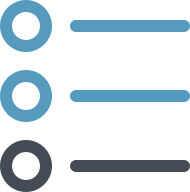
\includegraphics{images/_icons/alltutorials.png}}
\end{minipage}
\hfill
\begin{minipage}[t]{0.90\textwidth}
\vspace{-2mm}
\setlength{\parskip}{1em}
}{\end{minipage}
\end{mdframed}
\vspace{4mm}
}

% singlelab

\newenvironment{singlelab}{
\vspace{4mm}
\begin{mdframed}[topline=false, bottomline=false, rightline=false, leftline=false]
\begin{minipage}[t]{0.10\textwidth}
{$\:$ \\ \setkeys{Gin}{width=2em,keepaspectratio}
\includegraphics{images/_icons/singlelab.png}}
\end{minipage}
\hfill
\begin{minipage}[t]{0.90\textwidth}
\vspace{-2mm}
\setlength{\parskip}{1em}
}{\end{minipage}
\end{mdframed}
\vspace{4mm}
}

% alllabs

\newenvironment{alllabs}{
\vspace{4mm}
\begin{mdframed}[topline=false, bottomline=false, rightline=false, leftline=false]
\begin{minipage}[t]{0.10\textwidth}
{$\:$ \\ \setkeys{Gin}{width=2em,keepaspectratio}
\includegraphics{images/_icons/alllabs.png}}
\end{minipage}
\hfill
\begin{minipage}[t]{0.90\textwidth}
\vspace{-2mm}
\setlength{\parskip}{1em}
}{\end{minipage}
\end{mdframed}
\vspace{4mm}
}


% todo

\newenvironment{todo}{
\vspace{4mm}
\begin{mdframed}[%
    topline=true, bottomline=true, linecolor=oiY, linewidth=0.5pt,
    rightline=false, leftline=false,
    backgroundcolor=oiLY]
\begin{minipage}[t]{0.10\textwidth}
{$\:$ \\ \setkeys{Gin}{width=2em,keepaspectratio}
\includegraphics{images/_icons/to-do.png}}
\end{minipage}
\hfill
\begin{minipage}[t]{0.90\textwidth}
\vspace{-2mm}
\setlength{\parskip}{1em}
\noindent\textbf{\color{oiGray}\small\fontfamily{phv}\selectfont{\MakeUppercase{TO DO}}} $\:$ \\ \\
}{\end{minipage}
\end{mdframed}
\vspace{4mm}
}

% underconstruction

\newenvironment{underconstruction}{
\vspace{4mm}
\begin{mdframed}[%
    topline=true, bottomline=true, linecolor=oiR, linewidth=0.5pt,
    rightline=false, leftline=false,
    backgroundcolor=oiLR]
\begin{minipage}[t]{0.10\textwidth}
{$\:$ \\ \setkeys{Gin}{width=2em,keepaspectratio}
\includegraphics{images/_icons/under-construction.png}}
\end{minipage}
\hfill
\begin{minipage}[t]{0.90\textwidth}
\vspace{-2mm}
\setlength{\parskip}{1em}
\noindent\textbf{\color{oiR}\small\fontfamily{phv}\selectfont{\MakeUppercase{Under construction}}} $\:$ \\ \\
}{\end{minipage}
\end{mdframed}
\vspace{4mm}
}

% Cover image ------------------------------------------------------------------

\newenvironment{authorinfo}[1]
  {
  \begin{minipage}[c]{0.30\textwidth}
  {\setkeys{Gin}{width=12em,keepaspectratio}\includegraphics{#1}}
  \end{minipage} 
  \hfill
  \begin{minipage}[c]{0.60\textwidth}
  }
  {
  \end{minipage}
  }

% End ims-style.tex ------------------------------------------------------------
\ifLuaTeX
  \usepackage{selnolig}  % disable illegal ligatures
\fi
\usepackage[]{natbib}
\bibliographystyle{apalike}

\title{Introduction to Modern Statistics}
\author{Mine Çetinkaya-Rundel and Johanna Hardin}
\date{2021-05-08}

\begin{document}
\maketitle

{
\setcounter{tocdepth}{1}
\tableofcontents
}
\hypertarget{welcome}{%
\chapter*{Welcome}\label{welcome}}
\addcontentsline{toc}{chapter}{Welcome}

This is \emph{Introduction to Modern Statistics, First Edition}!
The source code for the book can be found \href{https://github.com/openintrostat/ims}{on GitHub}.

\begin{underconstruction}
First edition is currently under active development.
You can find the stable preliminary edition at \url{http://openintro-ims.netlify.app}.

This book is a revamped version of OpenIntro::Introduction to Statistics with Randomization and Simulation, the 1st edition of which can be accessed at \href{https://www.openintro.org/book/isrs/}{openintro.org/book/isrs}.

\end{underconstruction}

\vfill

\hypertarget{license}{%
\section*{License}\label{license}}
\addcontentsline{toc}{section}{License}

\begin{flushleft}
\includegraphics[width=0.1\linewidth]{images/by-nc-sa-4} \end{flushleft}

This online work is licensed under a \href{http://creativecommons.org/licenses/by-nc-sa/4.0/}{Creative Commons Attribution-NonCommercial-ShareAlike 4.0 International License}.
Visit \href{https://www.openintro.org/license/}{openintro.org/license} for more information about the license.

\hypertarget{authors}{%
\chapter*{Authors}\label{authors}}
\addcontentsline{toc}{chapter}{Authors}

\begin{authorinfo}{images/_authors/mine.png}
\href{http://mine-cr.com/}{Mine Çetinkaya-Rundel}

University of Edinburgh, Duke University, RStudio

\href{mailto:mine@openintro.org}{\nolinkurl{mine@openintro.org}}

\end{authorinfo}

Mine Çetinkaya-Rundel is Senior Lecturer in the School of Mathematics at University of Edinburgh, Data Scientist and Professional Educator at RStudio, and Associate Professor of the Practice position at the Department of Statistical Science at Duke University.
Mine's work focuses on innovation in statistics and data science pedagogy, with an emphasis on computing, reproducible research, student-centered learning, and open-source education as well as pedagogical approaches for enhancing retention of women and under-represented minorities in STEM.
Mine works on integrating computation into the undergraduate statistics curriculum, using reproducible research methodologies and analysis of real and complex datasets.
She also organizes \href{https://ww2.amstat.org/education/datafest/}{ASA DataFest}, an annual two-day competition in which teams of undergraduate students work to reveal insights into a rich and complex data set.
Mine works on the \href{openintro.org}{OpenIntro} project, whose mission is to make educational products that are free, transparent, and lower barriers to education.
As part of this project she co-authored three open-source introductory statistics textbooks.
She is also the creator and maintainer of \href{https://datasciencebox.org/}{datasciencebox.org} and she teaches the popular Statistics with R MOOC on Coursera.
\newline

\begin{authorinfo}{images/_authors/jo.png}
\href{https://research.pomona.edu/johardin/}{Johanna Hardin}

Pomona College

\href{mailto:jo.hardin@pomona.edu}{\nolinkurl{jo.hardin@pomona.edu}}

\end{authorinfo}

Jo Hardin is Professor of Mathematics and Statistics at Pomona College.
She collaborates with molecular biologists to create novel statistical methods for analyzing high throughput data.
She has also worked extensively in statistics and data science education, facilitating modern curricula for higher education instructors.
She was a co-author on the \href{https://www.amstat.org/asa/education/Curriculum-Guidelines-for-Undergraduate-Programs-in-Statistical-Science.aspx}{2014 ASA Curriculum Guidelines for Undergraduate Programs in Statistical Science}, and she writes on the blog \href{https://teachdatascience.com/}{teachdatascience.com}.
The best part of her job is collaborating with undergraduate students.
In her spare time, she loves reading, running, and breeding tortoises.

\hypertarget{preface}{%
\chapter*{Preface}\label{preface}}
\addcontentsline{toc}{chapter}{Preface}

We hope readers will take away three ideas from this book in addition to forming a foundation of statistical thinking and methods.

\begin{enumerate}
\def\labelenumi{\arabic{enumi}.}
\tightlist
\item
  Statistics is an applied field with a wide range of practical applications.
\item
  You don't have to be a math guru to learn from interesting, real data.
\item
  Data are messy, and statistical tools are imperfect. However, when you understand the strengths and weaknesses of these tools, you can use them to learn interesting things about the world.
\end{enumerate}

\hypertarget{textbook-overview}{%
\subsubsection*{Textbook overview}\label{textbook-overview}}
\addcontentsline{toc}{subsubsection}{Textbook overview}

\begin{enumerate}
\def\labelenumi{\arabic{enumi}.}
\tightlist
\item
  \textbf{Introduction to data.} Data structures, variables, summaries, graphics, and basic data collection techniques.
\item
  \textbf{Exploratory data analysis.} Data visualization and summarisation.
\item
  \textbf{Correlation and regression.} Visualizing relationships between many variables and descriptive summaries for quantifying the relationship between two variables.
\item
  \textbf{Multiple regression.} Descriptive summaries for quantifying the relationship between two variables.
\item
  \textbf{Foundations for inference.} Case studies are used to introduce the ideas of statistical inference with randomization and simulations.
\item
  \textbf{Inference for categorical data.} Inference for proportions using simulation and randomization techniques as well as the normal and chi-square distributions.
\item
  \textbf{Inference for numerical data.} Inference for one or two sample means using simulation and randomization techniques as well as the normal and F distributions.
\item
  \textbf{Inference for regression.} Extending inference techniques presented thus-far to regression settings.
\end{enumerate}

\hypertarget{examples-and-exercises}{%
\subsubsection*{Examples and exercises}\label{examples-and-exercises}}
\addcontentsline{toc}{subsubsection}{Examples and exercises}

Examples are provided to establish an understanding of how to apply methods.

\begin{workedexample}
This is an example.
When a question is asked here, where can the answer be found?

\begin{center}\rule{0.5\linewidth}{0.5pt}\end{center}

The answer can be found here, in the solution section of the example!

\end{workedexample}

When we think the reader should be ready to try determining the solution to an example, we frame it as Guided Practice.

\begin{guidedpractice}
The reader may check or learn the answer to any Guided Practice problem by reviewing the full solution in a footnote.\footnote{Guided Practice problems are intended to stretch your thinking, and you can check yourself by reviewing the footnote solution for any Guided Practice.}

\end{guidedpractice}

Exercises are also provided at the end of each section as well as review exercises at the end of each chapter.

\hypertarget{datasets}{%
\subsubsection*{Datasets}\label{datasets}}
\addcontentsline{toc}{subsubsection}{Datasets}

A large majority of the datasets used in the book can be found in various R packages.
Each time a new dataset is introduced in the narrative, a reference to the package like the one below is provided.
Many of these datasets are in the \href{http://openintrostat.github.io/openintro}{openintro} package that contains data sets used in \href{https://www.openintro.org/}{OpenIntro}'s open-source textbooks.\footnote{Mine Çetinkaya-Rundel, David Diez, Andrew Bray, Albert Kim, Ben Baumer, Chester Ismay and Christopher Barr (2020).
  openintro: Data Sets and Supplemental Functions from `OpenIntro' Textbooks and Labs.
  R package version 2.0.0.
  \url{https://github.com/OpenIntroStat/openintro}.}

\begin{data}
These data can be found in the \href{http://openintrostat.github.io/openintro}{openintro} package: \href{http://openintrostat.github.io/openintro/reference/textbooks.html}{\texttt{textbooks}}.

\end{data}

\hypertarget{computing-with-r}{%
\subsubsection*{Computing with R}\label{computing-with-r}}
\addcontentsline{toc}{subsubsection}{Computing with R}

The narrative and the exercises in the book are computing language agnostic, however while it's possible to learn about modern statistics without computing, it's not possible to apply it.
Therefore, we invite you to navigate the concepts you have learned in each chapter using the interactive R tutorials and the R labs that are included at the end of each chapter.

\textbf{Interactive R tutorials}

These are self-paced tutorials developed using the \href{https://rstudio.github.io/learnr/index.html}{learnr} package and you only need a browser to complete them.

\begin{alltutorials}
Each chapter comes with a tutorial which is listed like this, which is comprised of 3-5 lessons.

\end{alltutorials}

\begin{singletutorial}
Each of these lessons\ldots{}

\end{singletutorial}

\begin{singletutorial}
\ldots{} are listed like this.

\end{singletutorial}

You can also access the full list of tutorials supporting this book \href{https://openintrostat.github.io/ims-tutorials/}{here}.

\textbf{R labs}

Once you feel comfortable with the material in these tutorials, we also encourage you to apply what you've learned via the computational labs that are also linked at the end of each chapter.
These are data analysis case studies and they require access to \href{https://cran.r-project.org/}{R} and \href{https://rstudio.com/products/rstudio/}{RStudio}.
The first lab includes installation instructions.
If you'd rather not install the software, you can also try \href{https://rstudio.cloud/}{RStudio Cloud} for free.

\begin{singlelab}
Labs for each chapter are listed like this.

\end{singlelab}

\begin{alllabs}
And you can find the full list of labs supporting this textbook \href{http://openintrostat.github.io/oilabs-tidy/}{here}.

\end{alllabs}

\hypertarget{openintro-online-resources-and-getting-involved}{%
\subsubsection*{OpenIntro, online resources, and getting involved}\label{openintro-online-resources-and-getting-involved}}
\addcontentsline{toc}{subsubsection}{OpenIntro, online resources, and getting involved}

OpenIntro is an organization focused on developing free and affordable education materials.

We encourage anyone learning or teaching statistics to visit \href{http://www.openintro.org}{openintro.org} and get involved.

All OpenIntro resources are free and anyone is welcomed to use these online tools and resources with or without this textbook as a companion.

We value your feedback.
If there is a part of the project you especially like or think needs improvement, we want to hear from you.
For feedback on this specific book, you can open an issue \href{https://github.com/openintrostat/ims/issues}{on GitHub}.
You can also provide feedback on this book or any other OpenIntro resource via our contact form at \href{https://www.openintro.org/form/?f=contact}{openintro.org}.

\hypertarget{acknowledgements}{%
\subsubsection*{Acknowledgements}\label{acknowledgements}}
\addcontentsline{toc}{subsubsection}{Acknowledgements}

The \emph{OpenIntro} project would not have been possible without the dedication and volunteer hours of all those involved.
No one has received any monetary compensation from this project, and we hope you will join us in extending a huge \emph{thank you} to all those who volunteer with OpenIntro.

The authors would like to thank

\begin{itemize}
\tightlist
\item
  David Diez and Christopher Barr for their work on the 1st Edition of this book,
\item
  Ben Baumer and Andrew Bray for their contribution to the original vision for the revamp for the 2nd Edition as well as their work as original authors of the interactive tutorial content,
\item
  Yanina Bellini Saibene, Florencia~D'Andrea, and Roxana Noelia Villafañe for their work on creating the interactive tutorials in learnr,
\item
  Will Gray for conceptual diagrams,
\item
  Allison Theobold, Melinda Yager, and Randy Prium for their valuable feedback and review of the book,
\item
  Colin Rundel for technical help with conversion from LaTeX to R Markdown, and
\item
  Müge Çetinkaya and Meenal Patel for their design vision.
\end{itemize}

We would like to also thank the developers of the open-source tools that make the development and authoring of this book possible, e.g.~\href{https://bookdown.org/}{bookdown}, \href{https://tidyverse.org/}{tidyverse}, and \href{http://icons8.com/}{icons8}.

We are also grateful to the many teachers, students, and other readers who have helped improve OpenIntro resources through their feedback.

\hypertarget{part-introduction-to-data}{%
\part{Introduction to data}\label{part-introduction-to-data}}

\hypertarget{data-hello}{%
\chapter{Hello data}\label{data-hello}}

\begin{chapterintro}
Scientists seek to answer questions using rigorous methods and careful observations.
These observations -- collected from the likes of field notes, surveys, and experiments -- form the backbone of a statistical investigation and are called \textbf{data}.
Statistics is the study of how best to collect, analyze, and draw conclusions from data.
In this first chapter, we focus on both the properties of data and on the collection of data.

\end{chapterintro}

\hypertarget{case-study-stents-strokes}{%
\section{Case study: Using stents to prevent strokes}\label{case-study-stents-strokes}}

In this section we introduce a classic challenge in statistics: evaluating the efficacy of a medical treatment.
Terms in this section, and indeed much of this chapter, will all be revisited later in the text.
The plan for now is simply to get a sense of the role statistics can play in practice.

An experiment is designed to study the effectiveness of stents in treating patients at risk of stroke \citep{chimowitz2011stenting}.
Stents are small mesh tubes that are placed inside narrow or weak arteries to assist in patient recovery after cardiac events and reduce the risk of an additional heart attack or death.

Many doctors have hoped that there would be similar benefits for patients at risk of stroke.
We start by writing the principal question the researchers hope to answer:

\begin{quote}
Does the use of stents reduce the risk of stroke?
\end{quote}

The researchers who asked this question conducted an experiment with 451 at-risk patients.
Each volunteer patient was randomly assigned to one of two groups:

\begin{itemize}
\tightlist
\item
  \textbf{Treatment group}. Patients in the treatment group received a stent and medical management. The medical management included medications, management of risk factors, and help in lifestyle modification.
\item
  \textbf{Control group}. Patients in the control group received the same medical management as the treatment group, but they did not receive stents.
\end{itemize}

Researchers randomly assigned 224 patients to the treatment group and 227 to the control group.
In this study, the control group provides a reference point against which we can measure the medical impact of stents in the treatment group.

Researchers studied the effect of stents at two time points: 30 days after enrollment and 365 days after enrollment.
The results of 5 patients are summarized in Table \ref{tab:stentStudyResultsDF}.
Patient outcomes are recorded as \texttt{stroke} or \texttt{no\ event}, representing whether or not the patient had a stroke during that time period.

\begin{data}
The data from this study can be found in the \href{http://openintrostat.github.io/openintro}{openintro} package: \href{http://openintrostat.github.io/openintro/reference/stent30.html}{\texttt{stent30}} and \href{http://openintrostat.github.io/openintro/reference/stent365.html}{\texttt{stent365}}.

\end{data}

\begin{table}

\caption{\label{tab:stentStudyResultsDF}Results for five patients from the stent study.}
\centering
\begin{tabular}[t]{rlll}
\toprule
patient & group & 30 days & 365 days\\
\midrule
\cellcolor{gray!6}{1} & \cellcolor{gray!6}{treatment} & \cellcolor{gray!6}{no event} & \cellcolor{gray!6}{no event}\\
2 & treatment & stroke & stroke\\
\cellcolor{gray!6}{3} & \cellcolor{gray!6}{treatment} & \cellcolor{gray!6}{no event} & \cellcolor{gray!6}{no event}\\
4 & treatment & no event & no event\\
\cellcolor{gray!6}{5} & \cellcolor{gray!6}{control} & \cellcolor{gray!6}{no event} & \cellcolor{gray!6}{no event}\\
\bottomrule
\end{tabular}
\end{table}

It would be difficult to answer a question on the impact of stents on the occurance of strokes for \textbf{all} of the study patients using these \emph{individual} observations.
This question is better addressed by performing a statistical data analysis of \emph{all} of the observations.
Table \ref{tab:stentStudyResultsDFsummary} summarizes the raw data in a more helpful way.
In this table, we can quickly see what happened over the entire study.
For instance, to identify the number of patients in the treatment group who had a stroke within 30 days after the treatment, we look in the leftmost column (30 days), at the intersection of treatment and stroke: 33.
To identify the number of control patients who did not have a stroke after 365 days after receiving treatment, we look at the rightmost column (365 days), at the intersection of control and no event: 199.

\begin{table}

\caption{\label{tab:stentStudyResultsDFsummary}Descriptive statistics for the stent study.}
\centering
\begin{tabular}[t]{lrrrr}
\toprule
\multicolumn{1}{c}{ } & \multicolumn{2}{c}{30 days} & \multicolumn{2}{c}{365 days} \\
\cmidrule(l{3pt}r{3pt}){2-3} \cmidrule(l{3pt}r{3pt}){4-5}
 & stroke & no event & stroke & no event\\
\midrule
\cellcolor{gray!6}{treatment} & \cellcolor{gray!6}{33} & \cellcolor{gray!6}{191} & \cellcolor{gray!6}{45} & \cellcolor{gray!6}{179}\\
control & 13 & 214 & 28 & 199\\
\cellcolor{gray!6}{Total} & \cellcolor{gray!6}{46} & \cellcolor{gray!6}{405} & \cellcolor{gray!6}{73} & \cellcolor{gray!6}{378}\\
\bottomrule
\end{tabular}
\end{table}

\begin{guidedpractice}
Of the 224 patients in the treatment group, 45 had a stroke by the end of the first year.
Using these two numbers, compute the proportion of patients in the treatment group who had a stroke by the end of their first year.
(Note: answers to all Guided Practice exercises are provided in footnotes!)\footnote{The proportion of the 224 patients who had a stroke within 365 days: \(45/224 = 0.20.\)}

\end{guidedpractice}

We can compute summary statistics from the table to give us a better idea of how the impact of the stent treatment differed between the two groups.
A \textbf{summary statistic} is a single number summarizing data from a sample.
For instance, the primary results of the study after 1 year could be described by two summary statistics: the proportion of people who had a stroke in the treatment and control groups.

\begin{itemize}
\tightlist
\item
  Proportion who had a stroke in the treatment (stent) group: \(45/224 = 0.20 = 20\%.\)
\item
  Proportion who had a stroke in the control group: \(28/227 = 0.12 = 12\%.\)
\end{itemize}

These two summary statistics are useful in looking for differences in the groups, and we are in for a surprise: an additional 8\% of patients in the treatment group had a stroke!
This is important for two reasons.
First, it is contrary to what doctors expected, which was that stents would \emph{reduce} the rate of strokes.
Second, it leads to a statistical question: do the data show a ``real'' difference between the groups?

This second question is subtle.
Suppose you flip a coin 100 times.
While the chance a coin lands heads in any given coin flip is 50\%, we probably won't observe exactly 50 heads.
This type of variation is part of almost any type of data generating process.
It is possible that the 8\% difference in the stent study is due to this natural variation.
However, the larger the difference we observe (for a particular sample size), the less believable it is that the difference is due to chance.
So what we are really asking is the following: if in fact stents have no effect, how likely is it that would observe such a large difference?

While we don't yet have statistical tools to fully address this question on our own, we can comprehend the conclusions of the published analysis: there was compelling evidence of harm by stents in this study of stroke patients.

\textbf{Be careful:} Do not generalize the results of this study to all patients and all stents.
This study looked at patients with very specific characteristics who volunteered to be a part of this study and who may not be representative of all stroke patients.
In addition, there are many types of stents and this study only considered the self-expanding Wingspan stent (Boston Scientific).
However, this study does leave us with an important lesson: we should keep our eyes open for surprises.

\hypertarget{data-basics}{%
\section{Data basics}\label{data-basics}}

Effective presentation and description of data is a first step in most analyses.
This section introduces one structure for organizing data as well as some terminology that will be used throughout this book.

\hypertarget{observations-variables-and-data-matrices}{%
\subsection{Observations, variables, and data matrices}\label{observations-variables-and-data-matrices}}

Table \ref{tab:loan50-df} displays six rows of a data set for 50 randomly sampled loans offered through Lending Club, which is a peer-to-peer lending company.
This dataset will be referred to as \texttt{loan50}.

\begin{data}
The data can be found in the \href{http://openintrostat.github.io/openintro}{openintro} package: \href{http://openintrostat.github.io/openintro/reference/loans_full_schema.html}{\texttt{loan50}}.

\end{data}

Each row in the table represents a single loan.
The formal name for a row is a \textbf{case} or \index{unit of observation}\textbf{observational unit}.
The columns represent characteristics of each loan, where each column is referred to as a \textbf{variable}.
For example, the first row represents a loan of \$22,000 with an interest rate of 10.90\%, where the borrower is based in New Jersey (NJ) and has an income of \$59,000.

\begin{guidedpractice}
What is the grade of the first loan in Table \ref{tab:loan50-df}?
And what is the home ownership status of the borrower for that first loan?
Reminder: for these Guided Practice questions, you can check your answer in the footnote.\footnote{The loan's grade is B, and the borrower rents their residence.}

\end{guidedpractice}

In practice, it is especially important to ask clarifying questions to ensure important aspects of the data are understood.
For instance, it is always important to be sure we know what each variable means and its units of measurement.
Descriptions of the variables in the \texttt{loan50} dataset are given in Table \ref{tab:loan-50-variables}.

\begin{table}

\caption{\label{tab:loan50-df}Six rows from the `loan50` data set}
\centering
\begin{tabular}[t]{lrrrllrl}
\toprule
  & loan\_amount & interest\_rate & term & grade & state & total\_income & homeownership\\
\midrule
\cellcolor{gray!6}{1} & \cellcolor{gray!6}{22000} & \cellcolor{gray!6}{10.90} & \cellcolor{gray!6}{60} & \cellcolor{gray!6}{B} & \cellcolor{gray!6}{NJ} & \cellcolor{gray!6}{59000} & \cellcolor{gray!6}{rent}\\
2 & 6000 & 9.92 & 36 & B & CA & 60000 & rent\\
\cellcolor{gray!6}{3} & \cellcolor{gray!6}{25000} & \cellcolor{gray!6}{26.30} & \cellcolor{gray!6}{36} & \cellcolor{gray!6}{E} & \cellcolor{gray!6}{SC} & \cellcolor{gray!6}{75000} & \cellcolor{gray!6}{mortgage}\\
4 & 6000 & 9.92 & 36 & B & CA & 75000 & rent\\
\cellcolor{gray!6}{5} & \cellcolor{gray!6}{25000} & \cellcolor{gray!6}{9.43} & \cellcolor{gray!6}{60} & \cellcolor{gray!6}{B} & \cellcolor{gray!6}{OH} & \cellcolor{gray!6}{254000} & \cellcolor{gray!6}{mortgage}\\
\addlinespace
6 & 6400 & 9.92 & 36 & B & IN & 67000 & mortgage\\
\bottomrule
\end{tabular}
\end{table}

\begin{table}

\caption{\label{tab:loan-50-variables}Variables and their descriptions for the `loan50` data set.}
\centering
\begin{tabular}[t]{l>{\raggedright\arraybackslash}p{30em}}
\toprule
variable & description\\
\midrule
\cellcolor{gray!6}{\ttfamily{loan\_amount}} & \cellcolor{gray!6}{Amount of the loan received, in US dollars.}\\
\ttfamily{interest\_rate} & Interest rate on the loan, in an annual percentage.\\
\cellcolor{gray!6}{\ttfamily{term}} & \cellcolor{gray!6}{The length of the loan, which is always set as a whole number of months.}\\
\ttfamily{grade} & Loan grade, which takes a values A through G and represents the quality of the loan and its likelihood of being repaid.\\
\cellcolor{gray!6}{\ttfamily{state}} & \cellcolor{gray!6}{US state where the borrower resides.}\\
\addlinespace
\ttfamily{total\_income} & Borrower's total income, including any second income, in US dollars.\\
\cellcolor{gray!6}{\ttfamily{homeownership}} & \cellcolor{gray!6}{Indicates whether the person owns, owns but has a mortgage, or rents.}\\
\bottomrule
\end{tabular}
\end{table}

The data in Table \ref{tab:loan50-df} represent a \textbf{data frame}, which is a convenient and common way to organize data, especially if collecting data in a spreadsheet.
A data frame where each row is a unique case (observational unit), each column is to a variable, and each cell is a single value is commonly referred to as \textbf{tidy data} \citet{wickham2014}.

When recording data, use a tidy data frame unless you have a very good reason to use a different structure.
This structure allows new cases to be added as rows or new variables as new columns and facilitates visualization, summarization, and other statistical analyses.

\begin{guidedpractice}
The grades for assignments, quizzes, and exams in a course are often recorded in a gradebook that takes the form of a data frame.
How might you organize a course's grade data using a data frame?
Describe the observational units and variables.\footnote{There are multiple strategies that can be followed.
  One common strategy is to have each student represented by a row, and then add a column for each assignment, quiz, or exam.
  Under this setup, it is easy to review a single line to understand the grade history of a student.
  There should also be columns to include student information, such as one column to list student names.}

\end{guidedpractice}

\begin{guidedpractice}
We consider data for 3,142 counties in the United States, which includes the name of each county, the state where it resides, its population in 2017, the population change from 2010 to 2017, poverty rate, and nine additional characteristics.
How might these data be organized in a data frame?\footnote{Each county may be viewed as a case, and there are eleven pieces of information recorded for each case.
  A table with 3,142 rows and 14 columns could hold these data, where each row represents a county and each column represents a particular piece of information.}

\end{guidedpractice}

The data described in the Guided Practice above represents the \textbf{county} data set, which is shown as a data frame in Table \ref{tab:county-df}.
The variables as well as the variables in the dataset that did not fit in Table \ref{tab:county-df} are described in Table \ref{tab:county-variables}.

\begin{table}

\caption{\label{tab:county-df}Six observations and six variables from the `county` data set.}
\centering
\begin{tabular}[t]{llrrrl}
\toprule
name & state & pop2017 & pop\_change & unemployment\_rate & median\_edu\\
\midrule
\cellcolor{gray!6}{Autauga County} & \cellcolor{gray!6}{Alabama} & \cellcolor{gray!6}{55504} & \cellcolor{gray!6}{1.48} & \cellcolor{gray!6}{3.86} & \cellcolor{gray!6}{some\_college}\\
Baldwin County & Alabama & 212628 & 9.19 & 3.99 & some\_college\\
\cellcolor{gray!6}{Barbour County} & \cellcolor{gray!6}{Alabama} & \cellcolor{gray!6}{25270} & \cellcolor{gray!6}{-6.22} & \cellcolor{gray!6}{5.90} & \cellcolor{gray!6}{hs\_diploma}\\
Bibb County & Alabama & 22668 & 0.73 & 4.39 & hs\_diploma\\
\cellcolor{gray!6}{Blount County} & \cellcolor{gray!6}{Alabama} & \cellcolor{gray!6}{58013} & \cellcolor{gray!6}{0.68} & \cellcolor{gray!6}{4.02} & \cellcolor{gray!6}{hs\_diploma}\\
\addlinespace
Bullock County & Alabama & 10309 & -2.28 & 4.93 & hs\_diploma\\
\bottomrule
\end{tabular}
\end{table}

\begin{table}

\caption{\label{tab:county-variables}Variables and their descriptions for the `county` data set.}
\centering
\begin{tabular}[t]{l>{\raggedright\arraybackslash}p{30em}}
\toprule
variable & description\\
\midrule
\cellcolor{gray!6}{\ttfamily{name}} & \cellcolor{gray!6}{Name of county.}\\
\ttfamily{state} & Name of state.\\
\cellcolor{gray!6}{\ttfamily{pop2000}} & \cellcolor{gray!6}{Population in 2000.}\\
\ttfamily{pop2010} & Population in 2010.\\
\cellcolor{gray!6}{\ttfamily{pop2017}} & \cellcolor{gray!6}{Population in 2017.}\\
\addlinespace
\ttfamily{pop\_change} & Population change from 2010 to 2017 (in percent).\\
\cellcolor{gray!6}{\ttfamily{poverty}} & \cellcolor{gray!6}{Percent of population in poverty in 2017.}\\
\ttfamily{homeownership} & Homeownership rate, 2006-2010.\\
\cellcolor{gray!6}{\ttfamily{multi\_unit}} & \cellcolor{gray!6}{Multi-unit rate: percent of housing units that are in multi-unit structures, 2006-2010.}\\
\ttfamily{unemployment\_rate} & Unemployment rate in 2017.\\
\addlinespace
\cellcolor{gray!6}{\ttfamily{metro}} & \cellcolor{gray!6}{Whether the county contains a metropolitan area, taking one of the values `yes` or `no`.}\\
\ttfamily{median\_edu} & Median education level (2013-2017), taking one of the values `below\_hs`, `hs\_diploma`, `some\_college`, or `bachelors`.\\
\cellcolor{gray!6}{\ttfamily{per\_capita\_income}} & \cellcolor{gray!6}{Per capita (per person) income (2013-2017).}\\
\ttfamily{median\_hh\_income} & Median household income.\\
\cellcolor{gray!6}{\ttfamily{smoking\_ban}} & \cellcolor{gray!6}{Describes whether the type of county-level smoking ban in place in 2010, taking one of the values `none`, `partial`, or `comprehensive`.}\\
\bottomrule
\end{tabular}
\end{table}

\begin{data}
These data can be found in the \href{http://openintrostat.github.io/usdata}{usdata} package: \href{http://openintrostat.github.io/usdata/reference/county.html}{\texttt{county}}.

\end{data}

\hypertarget{variable-types}{%
\subsection{Types of variables}\label{variable-types}}

Examine the \texttt{unemployment\_rate}, \texttt{pop2017}, \texttt{state}, and \texttt{median\_edu} variables in the \texttt{county} data set.
Each of these variables is inherently different from the other three, yet some share certain characteristics.

First consider \texttt{unemployment\_rate}, which is said to be a \textbf{numerical} variable since it can take a wide range of numerical values, and it is sensible to add, subtract, or take averages with those values.
On the other hand, we would not classify a variable reporting telephone area codes as numerical since the average, sum, and difference of area codes doesn't have any clear meaning.
Instead, we would consider area codes as a categorical variable.

The \texttt{pop2017} variable is also numerical, although it seems to be a little different than \texttt{unemployment\_rate}.
This variable of the population count can only take whole non-negative numbers (0, 1, 2, \ldots).
For this reason, the population variable is said to be \textbf{discrete} since it can only take numerical values with jumps.
On the other hand, the unemployment rate variable is said to be \textbf{continuous}.

The variable \texttt{state} can take up to 51 values after accounting for Washington, DC: AL, AK, \ldots, and WY.
Because the responses themselves are categories, \texttt{state} is called a \textbf{categorical} variable, and the possible values (states) are called the variable's \textbf{levels} (e.g., DC, AL, AK, etc.) .

Finally, consider the \texttt{median\_edu} variable, which describes the median education level of county residents and takes values \texttt{below\_hs}, \texttt{hs\_diploma}, \texttt{some\_college}, or \texttt{bachelors} in each county.
This variable seems to be a hybrid: it is a categorical variable but the levels have a natural ordering.
A variable with these properties is called an \textbf{ordinal} variable, while a regular categorical variable without this type of special ordering is called a \textbf{nominal} variable.
To simplify analyses, any categorical variable in this book will be treated as a nominal (unordered) categorical variable.

\begin{figure}

{\centering \includegraphics[width=0.9\linewidth]{01-data-hello_files/figure-latex/variables-1} 

}

\caption{Breakdown of variables into their respective types.}\label{fig:variables}
\end{figure}

\begin{workedexample}
Data were collected about students in a statistics course.
Three variables were recorded for each student: number of siblings, student height, and whether the student had previously taken a statistics course.
Classify each of the variables as continuous numerical, discrete numerical, or categorical.

\begin{center}\rule{0.5\linewidth}{0.5pt}\end{center}

The number of siblings and student height represent numerical variables.
Because the number of siblings is a count, it is discrete.
Height varies continuously, so it is a continuous numerical variable.
The last variable classifies students into two categories -- those who have and those who have not taken a statistics course -- which makes this variable categorical.

\end{workedexample}

\index{data!stroke}

\begin{guidedpractice}
An experiment is evaluating the effectiveness of a new drug in treating migraines.
A \texttt{group} variable is used to indicate the experiment group for each patient: treatment or control.
The \texttt{num\_migraines} variable represents the number of migraines the patient experienced during a 3-month period.
Classify each variable as either numerical or categorical?\footnote{The \texttt{group} variable can take just one of two group names, making it categorical.
  The \texttt{num\_migraines} variable describes a count of the number of migraines, which is an outcome where basic arithmetic is sensible, which means this is numerical outcome; more specifically, since it represents a count, \texttt{num\_migraines} is a discrete numerical variable.}

\end{guidedpractice}

\hypertarget{variable-relations}{%
\subsection{Relationships between variables}\label{variable-relations}}

Many analyses are motivated by a researcher looking for a relationship between two or more variables.
A social scientist may like to answer some of the following questions:

\begin{quote}
Does a higher than average increase in county population tend to correspond to counties with higher or lower median household incomes?
\end{quote}

\begin{quote}
If homeownership is lower than the national average in one county, will the percent of housing units that are in multi-unit structures in that county tend to be above or below the national average?
\end{quote}

\begin{quote}
How much can the median education level explain the median household income for counties in the US?
\end{quote}

To answer these questions, data must be collected, such as the \texttt{county} data set shown in Table \ref{tab:county-df}.
Examining \index{summary statistic}\textbf{summary statistics} can provide numerical insights about the specifics of each of these questions.
Alternatively, graphs can be used to visually explore the data, potentially providing more insight than a summary statistic.

\index{scatterplot}\textbf{Scatterplots} are one type of graph used to study the relationship between two numerical variables.
Figure \ref{fig:county-multi-unit-homeownership} displays the relationship between the variables \texttt{homeownership} and \texttt{multi\_unit}, which is the percent of housing units that are in multi-unit structures (e.g., apartments, condos).
Each point on the plot represents a single county.
For instance, the highlighted dot corresponds to County 413 in the \texttt{county} data set: Chattahoochee County, Georgia, which has 39.4\% of housing units that are in multi-unit structures and a homeownership rate of 31.3\%.
The scatterplot suggests a relationship between the two variables: counties with a higher rate of housing units that are in multi-unit structures tend to have lower homeownership rates.
We might brainstorm as to why this relationship exists and investigate each idea to determine which are the most reasonable explanations.

\begin{figure}

{\centering \includegraphics[width=0.9\linewidth]{01-data-hello_files/figure-latex/county-multi-unit-homeownership-1} 

}

\caption{A scatterplot of homeownership versus the percent of housing units that are in multi-unit structures for US counties. The highlighted dot represents Chattahoochee County, Georgia, which has a multi-unit rate of 39.4\% and a homeownership rate of 31.3\%.}\label{fig:county-multi-unit-homeownership}
\end{figure}

The multi-unit and homeownership rates are said to be associated because the plot shows a discernible pattern.
When two variables show some connection with one another, they are called \textbf{associated} variables.

\begin{guidedpractice}
Examine the variables in the \texttt{loan50} data set, which are described in Table \ref{tab:loan-50-variables}.
Create two questions about possible relationships between variables in \texttt{loan50} that are of interest to you.\footnote{Two example questions: (1) What is the relationship between loan amount and total income?
  (2) If someone's income is above the average, will their interest rate tend to be above or below the average?}

\end{guidedpractice}

\begin{workedexample}
This example examines the relationship between the percent change in population from 2010 to 2017 and median household income for counties, which is visualized as a scatterplot in Figure \ref{fig:county-pop-change-med-hh-income}.
Are these variables associated?

\begin{center}\rule{0.5\linewidth}{0.5pt}\end{center}

The larger the median household income for a county, the higher the population growth observed for the county.
While it isn't true that every county with a higher median household income has a higher population growth, the trend in the plot is evident.
Since there is some relationship between the variables, they are associated.

\end{workedexample}

\begin{figure}

{\centering \includegraphics[width=0.9\linewidth]{01-data-hello_files/figure-latex/county-pop-change-med-hh-income-1} 

}

\caption{A scatterplot showing population chance against median household income. Owsley County of Kentucky, is highlighted, which lost 3.63\% of its population from 2010 to 2017 and had median household income of \$22,736.}\label{fig:county-pop-change-med-hh-income}
\end{figure}

Because there is a downward trend in Figure \ref{fig:county-multi-unit-homeownership} -- counties with more housing units that are in multi-unit structures are associated with lower homeownership -- these variables are said to be \textbf{negatively associated}.
A \textbf{positive association} is shown in the relationship between the \texttt{median\_hh\_income} and \texttt{pop\_change} variables in Figure \ref{fig:county-pop-change-med-hh-income}, where counties with higher median household income tend to have higher rates of population growth.

If two variables are not associated, then they are said to be \textbf{independent}.
That is, two variables are independent if there is no evident relationship between the two.

\begin{important}
\textbf{Associated or independent, not both.}

A pair of variables are either related in some way (associated) or not (independent).
No pair of variables is both associated and independent.

\end{important}

\hypertarget{explanatory-and-response-variables}{%
\subsection{Explanatory and response variables}\label{explanatory-and-response-variables}}

When we ask questions about the relationship between two variables, we sometimes also want to determine if the change in one variable causes a change in the other.
Consider the following rephrasing of an earlier question about the \texttt{county} data set:

\begin{quote}
If there is an increase in the median household income in a county, does this drive an increase in its population?
\end{quote}

In this question, we are asking whether one variable affects another.
If this is our underlying belief, then \emph{median household income} is the \textbf{explanatory variable} and the \emph{population change} is the \textbf{response variable} in the hypothesized relationship.\footnote{In some disciplines, it's customary to refer to the explanatory variable as the \textbf{independent variable} and the response variable as the \textbf{dependent variable}.
  However, this becomes confusing since a \emph{pair} of variables might be independent or dependent, so we avoid this language.}

\begin{important}
\textbf{Explanatory and response variables.}

When we suspect one variable might causally affect another, we label the first variable the explanatory variable and the second the response variable.
We also use the terms \textbf{explanatory} and \textbf{response} to describe variables where the \textbf{response} might be predicted using the \textbf{explanatory} even if there is no causal relationship.

explanatory variable \(\rightarrow\) \emph{might affect} \(\rightarrow\) response variable

For many pairs of variables, there is no hypothesized relationship, and these labels would not be applied to either variable in such cases.

\end{important}

Bear in mind that the act of labeling the variables in this way does nothing to guarantee that a causal relationship exists.
A formal evaluation to check whether one variable causes a change in another requires an experiment.

\hypertarget{observational-studies-and-experiments}{%
\subsection{Observational studies and experiments}\label{observational-studies-and-experiments}}

There are two primary types of data collection: experiments and observational studies.

When researchers want to evaluate the effect of particular traits, treatments, or conditions, they conduct an \textbf{experiment}.
For instance, we may suspect drinking a high-calorie energy drink will improve performance in a race.
To check if there really is a causal relationship between the explanatory variable (whether the runner drank an energy drink or not) and the response variable (the race time), researchers identify a sample of individuals and split them into groups.
The individuals in each group are \emph{assigned} a treatment.
When individuals are randomly assigned to a group, the experiment is called a \textbf{randomized experiment}.
Random assignment organizes the participants in a study into groups that are roughly equal on all aspects, thus allowing us to control for any confounding variables that might affect the outcome (e.g.~fitness level, racing experience, etc.).
For example, each runner in the experiment could be randomly assigned, perhaps by flipping a coin, into one of two groups: the first group receives a \textbf{placebo} (fake treatment, in this case a no-calorie drink) and the second group receives the high-calorie energy drink.
See the case study in Section \ref{case-study-stents-strokes} for another example of an experiment, though that study did not employ a placebo.

Researchers perform an \textbf{observational study} when they collect data in a way that does not directly interfere with how the data arise.
For instance, researchers may collect information via surveys, review medical or company records, or follow a \textbf{cohort} of many similar individuals to form hypotheses about why certain diseases might develop.
In each of these situations, researchers merely observe the data that arise.
In general, observational studies can provide evidence of a naturally occurring association between variables, but they cannot by themselves show a causal connection as they don't offer a mechanism for controlling for confounding variables.

\begin{important}
\textbf{Association} \(\neq\) \textbf{Causation.}

In general, association does not imply causation.
An advantage of a randomized experiment is that it is easier to establish causal relationships with such a study.
The main reason for this is that observational studies do not control for confounding variables, and hence establishing causal relationships with observational studies requires advanced statistical methods (that are beyond the scope of this book).
We will revisit this idea when we discuss experiments later in the book.

\end{important}

\hypertarget{chp1-review}{%
\section{Chapter review}\label{chp1-review}}

\hypertarget{summary}{%
\subsection{Summary}\label{summary}}

This chapter introduced you to the world of data.
Data can be organized in many ways but tidy data, where each row represents an observation and each column represents a variable, lends itself most easily to statistical analysis.
Many of the ideas from this chapter will be seen as we move on to doing full data analyses.
In the next chapter you're going to learn about how we can design studies to collect the data we need to make conclusions at the desired scope of inference.

\hypertarget{terms}{%
\subsection{Terms}\label{terms}}

We introduced the following terms in the chapter.
If you're not sure what some of these terms mean, we recommend you go back in the text and review their definitions.
We are purposefully presenting them in alphabetical order, instead of in order of appearance, so they will be a little more challenging to locate.
However you should be able to easily spot them as \textbf{bolded text}.

\begin{tabu} to \linewidth {>{\raggedright}X>{\raggedright}X>{\raggedright}X}
\toprule
\cellcolor{gray!6}{associated} & \cellcolor{gray!6}{experiment} & \cellcolor{gray!6}{ordinal}\\
case & explanatory variable & placebo\\
\cellcolor{gray!6}{categorical} & \cellcolor{gray!6}{independent} & \cellcolor{gray!6}{positive association}\\
cohort & level & randomized experiment\\
\cellcolor{gray!6}{continuous} & \cellcolor{gray!6}{negative association} & \cellcolor{gray!6}{response variable}\\
\addlinespace
data & nominal & summary statistic\\
\cellcolor{gray!6}{data frame} & \cellcolor{gray!6}{numerical} & \cellcolor{gray!6}{tidy data}\\
dependent & observational study & variable\\
\cellcolor{gray!6}{discrete} & \cellcolor{gray!6}{observational unit} & \cellcolor{gray!6}{}\\
\bottomrule
\end{tabu}

\hypertarget{chp1-exercises}{%
\section{Exercises}\label{chp1-exercises}}

\begin{enumerate}
\def\labelenumi{\arabic{enumi}.}
\item
  \textbf{Marvel Cinematic Universe films.}
  The data frame below contains information on Marvel Cinematic Universe films through the Infinity saga (a movie storyline spanning from Ironman in 2008 to Endgame in 2019).
  Box office totals are given in millions of US Dollars.
  How many observations and how many variables does this data frame have?\footnote{The data used in this exercise can be found in the \textbf{openintro} R package: \href{http://openintrostat.github.io/openintro/reference/mcu_films.html}{\texttt{mcu\_films}}.}

  \begin{table}
  \centering
  \begin{tabular}[t]{c|l|c|c|c|c|c|c}
  \hline
  \multicolumn{2}{c|}{ } & \multicolumn{2}{c|}{Length} & \multicolumn{2}{c|}{ } & \multicolumn{2}{c}{Gross} \\
  \cline{3-4} \cline{7-8}
    & Title & Hrs & Mins & Release Date & Opening Wknd US & US & World\\
  \hline
  \cellcolor{gray!6}{1} & \cellcolor{gray!6}{Iron Man} & \cellcolor{gray!6}{2} & \cellcolor{gray!6}{6} & \cellcolor{gray!6}{5/2/2008} & \cellcolor{gray!6}{98.62} & \cellcolor{gray!6}{319.03} & \cellcolor{gray!6}{585.8}\\
  \hline
  2 & The Incredible Hulk & 1 & 52 & 6/12/2008 & 55.41 & 134.81 & 264.77\\
  \hline
  \cellcolor{gray!6}{3} & \cellcolor{gray!6}{Iron Man 2} & \cellcolor{gray!6}{2} & \cellcolor{gray!6}{4} & \cellcolor{gray!6}{5/7/2010} & \cellcolor{gray!6}{128.12} & \cellcolor{gray!6}{312.43} & \cellcolor{gray!6}{623.93}\\
  \hline
  4 & Thor & 1 & 55 & 5/6/2011 & 65.72 & 181.03 & 449.33\\
  \hline
  \cellcolor{gray!6}{5} & \cellcolor{gray!6}{Captain America: The First Avenger} & \cellcolor{gray!6}{2} & \cellcolor{gray!6}{4} & \cellcolor{gray!6}{7/22/2011} & \cellcolor{gray!6}{65.06} & \cellcolor{gray!6}{176.65} & \cellcolor{gray!6}{370.57}\\
  \hline
  ... & ... & ... & ... & ... & ... & ... & ...\\
  \hline
  \cellcolor{gray!6}{23} & \cellcolor{gray!6}{Spiderman: Far from Home} & \cellcolor{gray!6}{2} & \cellcolor{gray!6}{9} & \cellcolor{gray!6}{7/2/2019} & \cellcolor{gray!6}{92.58} & \cellcolor{gray!6}{390.53} & \cellcolor{gray!6}{1131.93}\\
  \hline
  \end{tabular}
  \end{table}
\item
  \textbf{Cherry Blossom Run.}
  The data frame below contains information on runners in the 2017 Cherry Blossom Run, which is an annual road race that takes place in Washington, DC.
  Most runners participate in a 10-mile run while a smaller fraction take part in a 5k run or walk.
  How many observations and how many variables does this data frame have?\footnote{The data used in this exercise can be found in the \textbf{openintro} R package: \href{http://openintrostat.github.io/openintro/reference/run17.html}{\texttt{run17}}.}

  \begin{table}
   \centering
   \begin{tabular}[t]{l|l|l|l|c|l|c|c|c|l}
   \hline
     & Bib & Name & Sex & Age & City / Country & Net & Clock & Pace & Event\\
   \hline
   \cellcolor{gray!6}{1} & \cellcolor{gray!6}{6} & \cellcolor{gray!6}{Hiwot G.} & \cellcolor{gray!6}{F} & \cellcolor{gray!6}{21} & \cellcolor{gray!6}{Ethiopia} & \cellcolor{gray!6}{3217} & \cellcolor{gray!6}{3217} & \cellcolor{gray!6}{321} & \cellcolor{gray!6}{10 Mile}\\
   \hline
   2 & 22 & Buze D. & F & 22 & Ethiopia & 3232 & 3232 & 323 & 10 Mile\\
   \hline
   \cellcolor{gray!6}{3} & \cellcolor{gray!6}{16} & \cellcolor{gray!6}{Gladys K.} & \cellcolor{gray!6}{F} & \cellcolor{gray!6}{31} & \cellcolor{gray!6}{Kenya} & \cellcolor{gray!6}{3276} & \cellcolor{gray!6}{3276} & \cellcolor{gray!6}{327} & \cellcolor{gray!6}{10 Mile}\\
   \hline
   4 & 4 & Mamitu D. & F & 33 & Ethiopia & 3285 & 3285 & 328 & 10 Mile\\
   \hline
   \cellcolor{gray!6}{5} & \cellcolor{gray!6}{20} & \cellcolor{gray!6}{Karolina N.} & \cellcolor{gray!6}{F} & \cellcolor{gray!6}{35} & \cellcolor{gray!6}{Poland} & \cellcolor{gray!6}{3288} & \cellcolor{gray!6}{3288} & \cellcolor{gray!6}{328} & \cellcolor{gray!6}{10 Mile}\\
   \hline
   ... & ... & ... & ... & ... & ... & ... & ... & ... & ...\\
   \hline
   \cellcolor{gray!6}{19961} & \cellcolor{gray!6}{25153} & \cellcolor{gray!6}{Andres E.} & \cellcolor{gray!6}{M} & \cellcolor{gray!6}{33} & \cellcolor{gray!6}{Woodbridge, VA} & \cellcolor{gray!6}{5287} & \cellcolor{gray!6}{5334} & \cellcolor{gray!6}{1700} & \cellcolor{gray!6}{5K}\\
   \hline
   \end{tabular}
   \end{table}

\begin{verbatim}
#>      Time      
#>    6    2    2
\end{verbatim}
\item
  \textbf{Air pollution and birth outcomes, study components.}
  Researchers collected data to examine the relationship between air pollutants and preterm births in Southern California.
  During the study air pollution levels were measured by air quality monitoring stations.
  Specifically, levels of carbon monoxide were recorded in parts per million, nitrogen dioxide and ozone in parts per hundred million, and coarse particulate matter (PM\(_{10}\)) in \(\mu g/m^3\).
  Length of gestation data were collected on 143,196 births between the years 1989 and 1993, and air pollution exposure during gestation was calculated for each birth.
  The analysis suggested that increased ambient PM\(_{10}\) and, to a lesser degree, CO concentrations may be associated with the occurrence of preterm births. \citep{Ritz+Yu+Chapa+Fruin:2000}

  \begin{enumerate}
  \def\labelenumii{\alph{enumii}.}
  \item
    Identify the main research question of the study.
  \item
    Who are the subjects in this study, and how many are included?
  \item
    What are the variables in the study? Identify each variable as numerical or categorical. If numerical, state whether the variable is discrete or continuous. If categorical, state whether the variable is ordinal.
  \end{enumerate}
\item
  \textbf{Cheaters, study components.}
  Researchers studying the relationship between honesty, age and self-control conducted an experiment on 160 children between the ages of 5 and 15. Participants reported their age, sex, and whether they were an only child or not. The researchers asked each child to toss a fair coin in private and to record the outcome (white or black) on a paper sheet, and said they would only reward children who report white. \citep{Bucciol:2011}

  \begin{enumerate}
  \def\labelenumii{\alph{enumii}.}
  \item
    Identify the main research question of the study.
  \item
    Who are the subjects in this study, and how many are included?
  \item
    The study's findings can be summarized as follows: \emph{``Half the students were explicitly told not to cheat and the others were not given any explicit instructions. In the no instruction group probability of cheating was found to be uniform across groups based on child's characteristics. In the group that was explicitly told to not cheat, girls were less likely to cheat, and while rate of cheating didn't vary by age for boys, it decreased with age for girls.''} How many variables were recorded for each subject in the study in order to conclude these findings? State the variables and their types.
  \end{enumerate}
\item
  \textbf{Gamification and statistics, study components.}
  Gamification is the application of game-design elements and game principles in non-game contexts.
  In educational settings, gamification is often implemented as educational activities to solve problems by using characteristics of game elements.
  Researchers investigating the effects of gamification on learning statistics conducted a study where they split college students in a statistics class into four groups: (1) no reading exercises and no gamification, (2) reading exercises but no gamification, (3) gamification but no reading exercises, and (4) gamification and reading exercises.
  Students in all groups also attended lectures.
  Students in the class were from two majors: Electrical and Computer Engineering (n = 279) and Business Administration (n = 86).
  After their assigned learning experience, each student took a final evaluation comprised of 30 multiple choice question and their score was measured as the number of questions they answered correctly.
  The researchers considered student' gender, level of studies (first through fourth year) and academic major.
  Other variables considered were expertise in the English language and use of personal computers and games, both of which were measured on a scale of 1 (beginner) to 5 (proficient).
  The study found that gamification had a positive effect on student learning compared to traditional teaching methods involving lectures and reading exercises.
  They also found that the effect was larger for females and Engineering students.\citep{Legaki:2020}

  \begin{enumerate}
  \def\labelenumii{\alph{enumii}.}
  \item
    Identify the main research question of the study.
  \item
    Who were the subjects in this study, and how many were included?
  \item
    What are the variables in the study? Identify each variable as numerical or categorical. If numerical, state whether the variable is discrete or continuous. If categorical, state whether the variable is ordinal.
  \end{enumerate}
\item
  \textbf{Stealers, study components.}
  In a study of the relationship between socio-economic class and unethical behavior, 129 University of California undergraduates at Berkeley were asked to identify themselves as having low or high social-class by comparing themselves to others with the most (least) money, most (least) education, and most (least) respected jobs.
  They were also presented with a jar of individually wrapped candies and informed that the candies were for children in a nearby laboratory, but that they could take some if they wanted.
  After completing some unrelated tasks, participants reported the number of candies they had taken. \citep{Piff:2012}

  \begin{enumerate}
  \def\labelenumii{\alph{enumii}.}
  \item
    Identify the main research question of the study.
  \item
    Who were the subjects in this study, and how many were included?
  \item
    The study found that students who were identified as upper-class took more candy than others. How many variables were recorded for each subject in the study in order to conclude these findings? State the variables and their types.
  \end{enumerate}
\item
  \textbf{Migraine and acupuncture.} A migraine is a particularly painful type of headache, which patients sometimes wish to treat with acupuncture.
  To determine whether acupuncture relieves migraine pain, researchers conducted a randomized controlled study where 89 individuals who identified as female diagnosed with migraine headaches were randomly assigned to one of two groups: treatment or control.
  43 patients in the treatment group received acupuncture that is specifically designed to treat migraines. 46 patients in the control group received placebo acupuncture (needle insertion at non-acupoint locations).
  24 hours after patients received acupuncture, they were asked if they were pain free. Results are summarized in the contingency table below.
  Also provided is a figure from the original paper displaying the appropriate area (M) versus the inappropriate area (S) used in the treatment of migraine attacks.\footnote{The data used in this exercise can be found in the \textbf{openintro} R package: \href{http://openintrostat.github.io/openintro/reference/migraine.html}{\texttt{migraine}}.}

  \begin{table}
   \centering
   \begin{tabular}[t]{l|r|r}
   \hline
   Group & No & Yes\\
   \hline
   \cellcolor{gray!6}{Control} & \cellcolor{gray!6}{44} & \cellcolor{gray!6}{2}\\
   \hline
   Treatment & 33 & 10\\
   \hline
   \end{tabular}
   \end{table}

  \begin{enumerate}
  \def\labelenumii{\alph{enumii}.}
  \item
    What percent of patients in the treatment group were pain free 24 hours after receiving acupuncture?
  \item
    What percent were pain free in the control group?
  \item
    In which group did a higher percent of patients become pain free 24 hours after receiving acupuncture?
  \item
    Your findings so far might suggest that acupuncture is an effective treatment for migraines for all people who suffer from migraines.
    However this is not the only possible conclusion that can be drawn based on your findings so far.
    What is one other possible explanation for the observed difference between the percentages of patients that are pain free 24 hours after receiving acupuncture in the two groups?
  \item
    What are the explanatory and response variables in this study?
  \end{enumerate}
\item
  \textbf{Sinusitis and antibiotics.}
  Researchers studying the effect of antibiotic treatment for acute sinusitis compared to symptomatic treatments randomly assigned 166 adults diagnosed with acute sinusitis to one of two groups: treatment or control.
  Study participants received either a 10-day course of amoxicillin (an antibiotic) or a placebo similar in appearance and taste.
  The placebo consisted of symptomatic treatments such as acetaminophen, nasal decongestants, etc.
  At the end of the 10-day period, patients were asked if they experienced improvement in symptoms.
  The distribution of responses is summarized below.\footnote{The data used in this exercise can be found in the \textbf{openintro} R package: \href{http://openintrostat.github.io/openintro/reference/sinusitis.html}{\texttt{sinusitis}}.}

  \begin{table}
  \centering
  \begin{tabular}[t]{l|r|r}
  \hline
  Group & No & Yes\\
  \hline
  \cellcolor{gray!6}{Control} & \cellcolor{gray!6}{16} & \cellcolor{gray!6}{65}\\
  \hline
  Treatment & 19 & 66\\
  \hline
  \end{tabular}
  \end{table}

  \begin{enumerate}
  \def\labelenumii{\alph{enumii}.}
  \item
    What percent of patients in the treatment group experienced improvement in symptoms?
  \item
    What percent experienced improvement in symptoms in the control group?
  \item
    In which group did a higher percentage of patients experience improvement in symptoms?
  \item
    Your findings so far might suggest a real difference in the effectiveness of antibiotic and placebo treatments for improving symptoms of sinusitis. However this is not the only possible conclusion that can be drawn based on your findings so far. What is one other possible explanation for the observed difference between the percentages patients who experienced improvement in symptoms?
  \item
    What are the explanatory and response variables in this study?
  \end{enumerate}
\item
  \textbf{Daycare fines, study components.}
  Researchers tested the deterrence hypothesis which predicts that the introduction of a penalty will reduce the occurrence of the behavior subject to the fine, with the condition that the fine leaves everything else unchanged by instituting a fine for late pickup at daycare centers.
  For this study, they worked with 10 volunteer daycare centers that did not originally impose a fine to parents for picking up their kids late.
  They randomly selected 6 of these daycare centers and instituted a monetary fine (of a considerable amount) for picking up children late and then removed it.
  In the remaining 4 daycare centers no fine was introduced.
  The study period was divided into four: before the fine (weeks 1--4), the first 4 weeks with the fine (weeks 5-8), the last 8 weeks with fine (weeks 9--16), and the after fine period (weeks 17-20).
  Throughout the study, the number of kids who were picked up late was recorded each week for each daycare.
  The study found that the number of late-coming parents increased significantly when the fine was introduced, and no reduction occurred after the fine was removed.\footnote{The data used in this exercise can be found in the \textbf{openintro} R package: \href{http://openintrostat.github.io/openintro/reference/daycare_fines.html}{\texttt{daycare\_fines}}.} \citep{Gneezy:2000}

  \begin{table}
  \centering
  \begin{tabular}[t]{c|c|l|c|l}
  \hline
  center & week & group & late\_pickups & study\_period\\
  \hline
  \cellcolor{gray!6}{1} & \cellcolor{gray!6}{1} & \cellcolor{gray!6}{test} & \cellcolor{gray!6}{8} & \cellcolor{gray!6}{before fine}\\
  \hline
  1 & 2 & test & 8 & before fine\\
  \hline
  \cellcolor{gray!6}{1} & \cellcolor{gray!6}{3} & \cellcolor{gray!6}{test} & \cellcolor{gray!6}{7} & \cellcolor{gray!6}{before fine}\\
  \hline
  1 & 4 & test & 6 & before fine\\
  \hline
  \cellcolor{gray!6}{1} & \cellcolor{gray!6}{5} & \cellcolor{gray!6}{test} & \cellcolor{gray!6}{8} & \cellcolor{gray!6}{first 4 weeks with fine}\\
  \hline
  ... & ... & ... & ... & ...\\
  \hline
  \cellcolor{gray!6}{10} & \cellcolor{gray!6}{20} & \cellcolor{gray!6}{control} & \cellcolor{gray!6}{13} & \cellcolor{gray!6}{after fine}\\
  \hline
  \end{tabular}
  \end{table}

  \begin{enumerate}
  \def\labelenumii{\alph{enumii}.}
  \item
    Is this an observational study or an experiment? Explain your reasoning.
  \item
    What are the cases in this study and how many are included?
  \item
    What is the response variable in the study and what type of variable is it?
  \item
    What are the explanatory variables in the study and what types of variables are they?
  \end{enumerate}
\item
  \textbf{Efficacy of COVID-19 vaccine on adolescents, study components.}
  Results of a Phase 3 trial announced in March 2021 show that the Pfizer-BioNTech COVID-19 vaccine demonstrated 100\% efficacy and robust antibody responses on 12 to 15 years old adolescents with or without prior evidence of SARS-CoV-2 infection. In this trial 2,260 adolescents were randomly assigned to two groups: one group got the vaccine (n = 1,131) and the other got a placebo (n = 1,129). While 18 cases of COVID-19 were observed in the placebo group, none were observed in the vaccine group.\footnote{The data used in this exercise can be found in the \textbf{openintro} R package: \href{http://openintrostat.github.io/openintro/reference/biontech_adolescents.html}{\texttt{biontech\_adolescents}}.} \citep{Pfizer:2021}

  \begin{enumerate}
  \def\labelenumii{\alph{enumii}.}
  \item
    Is this an observational study or an experiment? Explain your reasoning.
  \item
    What are the cases in this study and how many are included?
  \item
    What is the response variable in the study and what type of variable is it?
  \item
    What are the explanatory variables in the study and what types of variables are they?
  \end{enumerate}
\item
  \textbf{Palmer penguins.} Data were collected on 344 penguins living on three islands (Torgersen, Biscoe, and Dream) in the Palmer Archipelago, Antarctica.
  In addition to which island each penguin lives on, the data contains information on the species of the penguin (\emph{Adelie}, \emph{Chinstrap}, or \emph{Gentoo}), its bill length, bill depth, and flipper length (measured in millimeters), its body mass (measured in grams), and the sex of the penguin (female or male).\footnote{The data used in this exercise can be found in the \textbf{palmerpenguins} R package: \href{https://allisonhorst.github.io/palmerpenguins/reference/penguins.html}{\texttt{penguins}}.} Bill length and depth are measured as shown in the image.\footnote{Artwork by \href{https://twitter.com/allison_horst}{Allison Horst}.}

  \begin{enumerate}
  \def\labelenumii{\alph{enumii}.}
  \tightlist
  \item
    How many cases were included in the data?
  \item
    How many numerical variables are included in the data? Indicate what they are, and if they are continuous or discrete.
  \item
    How many categorical variables are included in the data, and what are they? List the corresponding levels (categories) for each.
  \end{enumerate}
\item
  \textbf{Smoking habits of UK residents.}
  A survey was conducted to study the smoking habits of 1,691 UK residents. Below is a data frame displaying a portion of the data collected in this survey.
  A blank cell indicates that \footnote{The data used in this exercise can be found in the \textbf{openintro} R package: \href{http://openintrostat.github.io/openintro/reference/smoking.html}{\texttt{smoking}}.}

  \begin{table}
   \centering
   \begin{tabular}[t]{l|l|l|l|c|l|c|c}
   \hline
   \multicolumn{6}{c|}{ } & \multicolumn{2}{c}{amount} \\
   \cline{7-8}
     & sex & age & marital\_status & gross\_income & smoke & weekend & weekday\\
   \hline
   \cellcolor{gray!6}{1} & \cellcolor{gray!6}{Female} & \cellcolor{gray!6}{61} & \cellcolor{gray!6}{Married} & \cellcolor{gray!6}{2,600 to 5,200} & \cellcolor{gray!6}{No} & \cellcolor{gray!6}{} & \cellcolor{gray!6}{}\\
   \hline
   2 & Female & 61 & Divorced & 10,400 to 15,600 & Yes & 5 & 4\\
   \hline
   \cellcolor{gray!6}{3} & \cellcolor{gray!6}{Female} & \cellcolor{gray!6}{69} & \cellcolor{gray!6}{Widowed} & \cellcolor{gray!6}{5,200 to 10,400} & \cellcolor{gray!6}{No} & \cellcolor{gray!6}{} & \cellcolor{gray!6}{}\\
   \hline
   4 & Female & 50 & Married & 5,200 to 10,400 & No &  & \\
   \hline
   \cellcolor{gray!6}{5} & \cellcolor{gray!6}{Male} & \cellcolor{gray!6}{31} & \cellcolor{gray!6}{Single} & \cellcolor{gray!6}{10,400 to 15,600} & \cellcolor{gray!6}{Yes} & \cellcolor{gray!6}{10} & \cellcolor{gray!6}{20}\\
   \hline
   ... & ... & ... & ... & ... & ... &  & \\
   \hline
   \cellcolor{gray!6}{1691} & \cellcolor{gray!6}{Male} & \cellcolor{gray!6}{49} & \cellcolor{gray!6}{Divorced} & \cellcolor{gray!6}{Above 36,400} & \cellcolor{gray!6}{Yes} & \cellcolor{gray!6}{15} & \cellcolor{gray!6}{10}\\
   \hline
   \end{tabular}
   \end{table}

  \begin{enumerate}
  \def\labelenumii{\alph{enumii}.}
  \item
    What does each row of the data frame represent?
  \item
    How many participants were included in the survey?
  \item
    Indicate whether each variable in the study is numerical or categorical. If numerical, identify as continuous or discrete. If categorical, indicate if the variable is ordinal.
  \end{enumerate}
\item
  \textbf{US Airports.}
  The visualization below shows the geographical distribution of airports in the contiguous United States and Washington, DC.
  This visualization was constructed based on a dataset where each observation is an airport.\footnote{The data used in this exercise can be found in the \textbf{airports} R package: \href{http://openintrostat.github.io/airports/reference/usairports.html}{\texttt{usairports}}.}

  \begin{center}\includegraphics[width=1\linewidth]{01-data-hello_files/figure-latex/unnamed-chunk-22-1} \end{center}

  \begin{enumerate}
  \def\labelenumii{\alph{enumii}.}
  \item
    List the variables you believe were necessary to create this visualization.
  \item
    Indicate whether each variable in the study is numerical or categorical. If numerical, identify as continuous or discrete. If categorical, indicate if the variable is ordinal.
  \end{enumerate}
\item
  \textbf{UN Votes.}
  The visualization below shows voting patterns the United States, Canada, and Mexico in the United Nations General Assembly on a variety of issues.
  Specifically, for a given year between 1946 and 2019, it displays the percentage of roll calls in which the country voted yes for each issue.
  This visualization was constructed based on a dataset where each observation is a country/year pair.\footnote{The data used in this exercise can be found in the \href{https://cran.r-project.org/web/packages/unvotes/index.html}{\textbf{unvotes}} package.}

  \begin{center}\includegraphics[width=1\linewidth]{01-data-hello_files/figure-latex/unnamed-chunk-23-1} \end{center}

  \begin{enumerate}
  \def\labelenumii{\alph{enumii}.}
  \item
    List the variables used in creating this visualization.
  \item
    Indicate whether each variable in the study is numerical or categorical. If numerical, identify as continuous or discrete. If categorical, indicate if the variable is ordinal.
  \end{enumerate}
\item
  \textbf{UK baby names.}
  The visualization below shows the number of baby girls born in the United Kingdom (comprised of England \& Wales, Northern Ireland, and Scotland) who were given the name ``Fiona'' over the years.\footnote{The data used in this exercise can be found in the \textbf{ukbabynames} R package: \href{https://mine-cetinkaya-rundel.github.io/ukbabynames/reference/ukbabynames.html}{\texttt{ukbabynames}}.}

  \begin{center}\includegraphics[width=1\linewidth]{01-data-hello_files/figure-latex/unnamed-chunk-24-1} \end{center}

  \begin{enumerate}
  \def\labelenumii{\alph{enumii}.}
  \item
    List the variables you believe were necessary to create this visualization.
  \item
    Indicate whether each variable in the study is numerical or categorical. If numerical, identify as continuous or discrete. If categorical, indicate if the variable is ordinal.
  \end{enumerate}
\item
  \textbf{Shows on Netflix.}
  The visualization below shows the distribution of ratings of TV shows on Netflix (a streaming entertainment service) based on the decade they were released in and the country they were produced in. In the dataset, each observation is a TV show.\footnote{The data used in this exercise can be found in the \textbf{tidytuesdayR} R package: \href{https://github.com/rfordatascience/tidytuesday/blob/master/data/2021/2021-04-20/readme.md}{\texttt{netflix\_titles}}.}

  \begin{center}\includegraphics[width=1\linewidth]{01-data-hello_files/figure-latex/unnamed-chunk-25-1} \end{center}

  \begin{enumerate}
  \def\labelenumii{\alph{enumii}.}
  \item
    List the variables you believe were necessary to create this visualization.
  \item
    Indicate whether each variable in the study is numerical or categorical. If numerical, identify as continuous or discrete. If categorical, indicate if the variable is ordinal.
  \end{enumerate}
\item
  \textbf{Stanford Open Policing.}
  The Stanford Open Policing project gathers, analyzes, and releases records from traffic stops by law enforcement agencies across the United States. Their goal is to help researchers, journalists, and policy makers investigate and improve interactions between police and the public. The following is an excerpt from a summary table created based off of the data collected as part of this project. \citep{pierson2017large}

  \begin{table}
   \centering
   \begin{tabular}[t]{l|l|l|c|c|c}
   \hline
   \multicolumn{2}{c|}{ } & \multicolumn{2}{c|}{Driver} & \multicolumn{2}{c}{Car} \\
   \cline{3-4} \cline{5-6}
   County & State & Race / Ethnicity & Arrest rate & Stops / year & Search rate\\
   \hline
   \cellcolor{gray!6}{Apache County} & \cellcolor{gray!6}{AZ} & \cellcolor{gray!6}{Black} & \cellcolor{gray!6}{0.016} & \cellcolor{gray!6}{266} & \cellcolor{gray!6}{0.077}\\
   \hline
   Apache County & AZ & Hispanic & 0.018 & 1008 & 0.053\\
   \hline
   \cellcolor{gray!6}{Apache County} & \cellcolor{gray!6}{AZ} & \cellcolor{gray!6}{White} & \cellcolor{gray!6}{0.006} & \cellcolor{gray!6}{6322} & \cellcolor{gray!6}{0.017}\\
   \hline
   Cochise County & AZ & Black & 0.015 & 1169 & 0.047\\
   \hline
   \cellcolor{gray!6}{Cochise County} & \cellcolor{gray!6}{AZ} & \cellcolor{gray!6}{Hispanic} & \cellcolor{gray!6}{0.01} & \cellcolor{gray!6}{9453} & \cellcolor{gray!6}{0.037}\\
   \hline
   Cochise County & AZ & White & 0.008 & 10826 & 0.024\\
   \hline
   \cellcolor{gray!6}{...} & \cellcolor{gray!6}{...} & \cellcolor{gray!6}{...} & \cellcolor{gray!6}{...} & \cellcolor{gray!6}{...} & \cellcolor{gray!6}{...}\\
   \hline
   Wood County & WI & Black & 0.098 & 16 & 0.244\\
   \hline
   \cellcolor{gray!6}{Wood County} & \cellcolor{gray!6}{WI} & \cellcolor{gray!6}{Hispanic} & \cellcolor{gray!6}{0.029} & \cellcolor{gray!6}{27} & \cellcolor{gray!6}{0.036}\\
   \hline
   Wood County & WI & White & 0.029 & 1157 & 0.033\\
   \hline
   \end{tabular}
   \end{table}

  \begin{enumerate}
  \def\labelenumii{\alph{enumii}.}
  \item
    What variables were collected on each individual traffic stop in order to create to the summary table above?
  \item
    State whether each variable is numerical or categorical. If numerical, state whether it is continuous or discrete. If categorical, state whether it is ordinal or not.
  \item
    Suppose we wanted to evaluate whether vehicle search rates are different for drivers of different races. In this analysis, which variable would be the response variable and which variable would be the explanatory variable?
  \end{enumerate}
\item
  \textbf{Space launches.}
  The following summary table shows the number of space launches in the US by the type of launching agency and the outcome of the launch (success or failure).\footnote{The data used in this exercise comes from the \href{https://www.openintro.org/go?id=textbook-space-launches-data\&referrer=ims0_html}{JSR Launch Vehicle Database, 2019 Feb 10 Edition}.}

  \begin{table}
   \centering
   \begin{tabular}[t]{l|r|r|r|r}
   \hline
   \multicolumn{1}{c|}{ } & \multicolumn{2}{c|}{1957 - 1999} & \multicolumn{2}{c}{2000-2018} \\
   \cline{2-3} \cline{4-5}
    & Failure & Success & Failure & Success\\
   \hline
   \cellcolor{gray!6}{Privste} & \cellcolor{gray!6}{13} & \cellcolor{gray!6}{295} & \cellcolor{gray!6}{10} & \cellcolor{gray!6}{562}\\
   \hline
   State & 281 & 3751 & 33 & 711\\
   \hline
   \cellcolor{gray!6}{Startup} & \cellcolor{gray!6}{0} & \cellcolor{gray!6}{0} & \cellcolor{gray!6}{5} & \cellcolor{gray!6}{65}\\
   \hline
   \end{tabular}
   \end{table}

  \begin{enumerate}
  \def\labelenumii{\alph{enumii}.}
  \item
    What variables were collected on each launch in order to create to the summary table above?
  \item
    State whether each variable is numerical or categorical. If numerical, state whether it is continuous or discrete. If categorical, state whether it is ordinal or not.
  \item
    Suppose we wanted to study how the success rate of launches vary between launching agencies and over time. In this analysis, which variable would be the response variable and which variable would be the explanatory variable?
  \end{enumerate}
\item
  \textbf{Pet names.}
  The city of Seattle, WA has an open data portal that includes pets registered in the city. For each registered pet, we have information on the pet's name and species.
  The following visualization plots the proportion of dogs with a given name versus the proportion of cats with the same name. The 20 most common cat and dog names are displayed.
  The diagonal line on the plot is the \(x = y\) line; if a name appeared on this line, the name's popularity would be exactly the same for dogs and cats.\footnote{The data used in this exercise can be found in the \textbf{openintro} R package: \href{http://openintrostat.github.io/openintro/reference/seattlepets.html}{\texttt{seattlepets}}.}

  \begin{center}\includegraphics[width=0.9\linewidth]{01-data-hello_files/figure-latex/unnamed-chunk-28-1} \end{center}

  \begin{enumerate}
  \def\labelenumii{\alph{enumii}.}
  \item
    Are these data collected as part of an experiment or an observational study?
  \item
    What is the most common dog name? What is the most common cat name?
  \item
    What names are more common for cats than dogs?
  \item
    Is the relationship between the two variables positive or negative? What does this mean in context of the data?
  \end{enumerate}
\item
  \textbf{Stressed out in an elevator.}
  In a study evaluating the relationship between stress and muscle cramps, half the subjects are randomly assigned to be exposed to increased stress by being placed into an elevator that falls rapidly and stops abruptly and the other half are left at no or baseline stress.

  \begin{enumerate}
  \def\labelenumii{\alph{enumii}.}
  \item
    What type of study is this?
  \item
    Can this study be used to conclude a causal relationship between increased stress and muscle cramps?
  \end{enumerate}
\end{enumerate}

\hypertarget{data-design}{%
\chapter{Study design}\label{data-design}}

\begin{chapterintro}
Before digging in to the details of working with data, we stop to think about how data come to be.
That is, if the data are to be used to make broad and complete conclusions, then it is important to understand who or what the data represent.
One important aspect of data provenance is sampling.
Knowing how the observational units were selected from a larger entity will allow for generalizations back to the population from which the data were randomly selected.
Additionally, by understanding the structure of the study, causal relationships can be separated from those relationships which are only correlated.
A good question to ask oneself before working with the data at all is,``How were these observations collected?'' You will learn a lot about the data by understanding its source.

\end{chapterintro}

\hypertarget{sampling-principles-strategies}{%
\section{Sampling principles and strategies}\label{sampling-principles-strategies}}

The first step in conducting research is to identify topics or questions that are to be investigated.
A clearly laid out research question is helpful in identifying what subjects or cases should be studied and what variables are important.
It is also important to consider \emph{how} data are collected so that they are reliable and help achieve the research goals.

\hypertarget{populations-and-samples}{%
\subsection{Populations and samples}\label{populations-and-samples}}

Consider the following three research questions:

\begin{enumerate}
\def\labelenumi{\arabic{enumi}.}
\tightlist
\item
  What is the average mercury content in swordfish in the Atlantic Ocean?
\item
  Over the last five years, what is the average time to complete a degree for Duke undergrads?
\item
  Does a new drug reduce the number of deaths in patients with severe heart disease?
\end{enumerate}

Each research question refers to a target \textbf{population}.
In the first question, the target population is all swordfish in the Atlantic ocean, and each fish represents a case.
Often times, it is not feasible to collect data for every case in a population.
This is generally because it is too expensive to collect data for the entire population, but it might also be because it is difficult or impossible to identify the entire population.
Instead, a sample is taken.
A \textbf{sample} is the data you have.
Ideally, a sample is a small fraction of the population.
For instance, 60 swordfish (or some other number) in the population might be selected, and this sample data may be used to provide an estimate of the population average and answer the research question.

\begin{guidedpractice}
For the second and third questions above, identify the target population and what represents an individual case.\footnote{The question \emph{``Over the last five years, what is the average time to complete a degree for Duke undergrads?''} is only relevant to students who complete their degree; the average cannot be computed using a student who never finished their degree.
  Thus, only Duke undergrads who graduated in the last five years represent cases in the population under consideration.
  Each such student is an individual case.
  For the question \emph{``Does a new drug reduce the number of deaths in patients with severe heart disease?''}, a person with severe heart disease represents a case.
  The population includes all people with severe heart disease.}

\end{guidedpractice}

\hypertarget{parameters-and-statistics}{%
\subsection{Parameters and statistics}\label{parameters-and-statistics}}

In the majority of statistical analysis procedures, the research question at hand boils down to understanding a numerical summary.
The number (or set of numbers) may be a quantity you are already familiar with (like the average) or it may be something you learn through this text (like the slope and intercept from a least squares model, provided in Section \ref{least-squares-regression}).

In theory, the numerical summary, however, can be calculated on either the sample of observation or the entire population.
Measuring every single unit in the population is usually prohibitive (so the parameter is very rarely calculated), but one can conceptualize calculating the average income of all adults in Argentina, for example, if one were all knowing.

We use specific terms in order to differentiate when a number is being calculated on a sample of data (\textbf{statistic}) and when it is being calculated or considered for calculation on the entire population (\textbf{parameter}).
The terms statistic and parameter are useful for communicating claims and models and will be used extensively in later chapters which delve into making inference on populations.

\hypertarget{anecdotal-evidence}{%
\subsection{Anecdotal evidence}\label{anecdotal-evidence}}

\index{bias}

Consider the following possible responses to the three research questions:

\begin{enumerate}
\def\labelenumi{\arabic{enumi}.}
\tightlist
\item
  A man on the news got mercury poisoning from eating swordfish, so the average mercury concentration in swordfish must be dangerously high.
\item
  I met two students who took more than 7 years to graduate from Duke, so it must take longer to graduate at Duke than at many other colleges.
\item
  My friend's dad had a heart attack and died after they gave him a new heart disease drug, so the drug must not work.
\end{enumerate}

Each conclusion is based on data.
However, there are two problems.
First, the data only represent one or two cases.
Second, and more importantly, it is unclear whether these cases are actually representative of the population.
Data collected in this haphazard fashion are called \textbf{anecdotal evidence}.

\begin{important}
\textbf{Anecdotal evidence.}

Be careful of data collected in a haphazard fashion.
Such evidence may be true and verifiable, but it may only represent extraordinary cases and therefore not be a good representation of the population.

\end{important}

\begin{figure}

{\centering 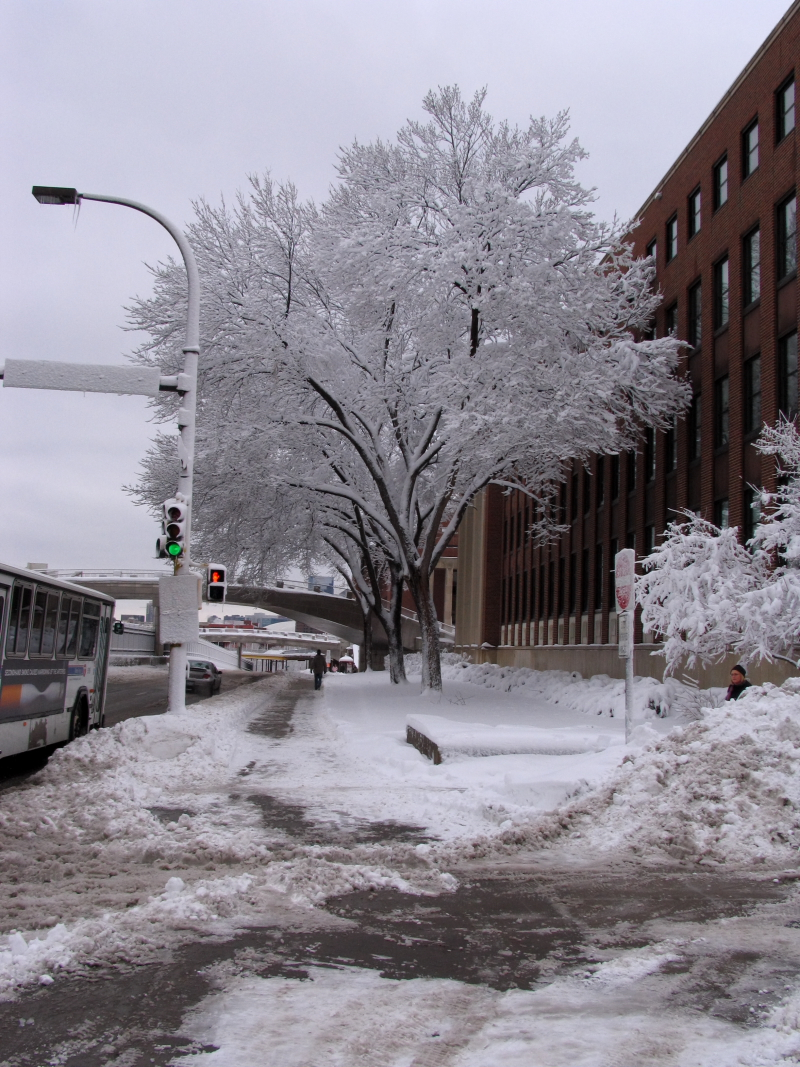
\includegraphics[width=0.5\linewidth]{images/mn-winter/mn-winter} 

}

\caption{In February 2010, some media pundits cited one large snow storm as evidence against global warming. As comedian Jon Stewart pointed out, "It is one storm, in one region, of one country."}\label{fig:mn-winter}
\end{figure}

Anecdotal evidence typically is composed of unusual cases that we recall based on their striking characteristics.
For instance, we are more likely to remember the two people we met who took 7 years to graduate than the six others who graduated in four years.
Instead of looking at the most unusual cases, we should examine a sample of many cases that better represent the population.

\hypertarget{sampling-from-a-population}{%
\subsection{Sampling from a population}\label{sampling-from-a-population}}

\index{random sample} \index{bias}

We might try to estimate the time to graduation for Duke undergraduates in the last five years by collecting a sample of graduates.
All graduates in the last five years represent the \emph{population}\index{population}, and graduates who are selected for review are collectively called the \emph{sample}\index{sample}.
In general, we always seek to \emph{randomly} select a sample from a population.
The most basic type of random selection is equivalent to how raffles are conducted.
For example, in selecting graduates, we could write each graduate's name on a raffle ticket and draw 10 tickets.
The selected names would represent a random sample of 10 graduates.

\begin{figure}

{\centering \includegraphics[width=0.8\linewidth]{02-data-design_files/figure-latex/pop-to-sample-1} 

}

\caption{In this graphic, 10 graduates are randomly selected from the population to be included in the sample.}\label{fig:pop-to-sample}
\end{figure}

\begin{workedexample}
Suppose we ask a student who happens to be majoring in nutrition to select several graduates for the study.
What kind of students do you think they might collect?
Do you think their sample would be representative of all graduates?

\begin{center}\rule{0.5\linewidth}{0.5pt}\end{center}

Perhaps they would pick a disproportionate number of graduates from health-related fields.
Or perhaps their selection would be a good representation of the population.
When selecting samples by hand, we run the risk of picking a \textbf{biased} sample, even if our bias is unintended.

\end{workedexample}

\begin{figure}

{\centering \includegraphics[width=0.8\linewidth]{02-data-design_files/figure-latex/pop-to-sub-sample-graduates-1} 

}

\caption{Asked to pick a sample of graduates, a nutrition major might inadvertently pick a disproportionate number of graduates from health-related majors.}\label{fig:pop-to-sub-sample-graduates}
\end{figure}

If someone was permitted to pick and choose exactly which graduates were included in the sample, it is entirely possible that the sample would overrepresent that person's interests, which may be entirely unintentional.
This introduces \textbf{bias} into a sample.
Sampling randomly helps resolve this problem.
The most basic random sample is called a \textbf{simple random sample}, and is equivalent to using a raffle to select cases.
This means that each case in the population has an equal chance of being included and there is no implied connection between the cases in the sample.

The act of taking a simple random sample helps minimize bias.
However, bias can crop up in other ways.
Even when people are picked at random, e.g., for surveys, caution must be exercised if the \textbf{non-response rate}\index{non-response rate} is high.
For instance, if only 30\% of the people randomly sampled for a survey actually respond, then it is unclear whether the results are \textbf{representative} of the entire population.
This \textbf{non-response bias}\index{non-response bias} can skew results.

\begin{figure}

{\centering \includegraphics[width=0.8\linewidth]{02-data-design_files/figure-latex/survey-sample-1} 

}

\caption{Due to the possibility of non-response, surveys studies may only reach a certain group within the population. It is difficult, and often times impossible, to completely fix this problem.}\label{fig:survey-sample}
\end{figure}

Another common downfall is a \textbf{convenience sample} \index{convenience sample}, where individuals who are easily accessible are more likely to be included in the sample.
For instance, if a political survey is done by stopping people walking in the Bronx, this will not represent all of New York City.
It is often difficult to discern what sub-population a convenience sample represents.

\begin{guidedpractice}
We can easily access ratings for products, sellers, and companies through websites.
These ratings are based only on those people who go out of their way to provide a rating.
If 50\% of online reviews for a product are negative, do you think this means that 50\% of buyers are dissatisfied with the product?
Why or why not?\footnote{Answers will vary.
  From our own anecdotal experiences, we believe people tend to rant more about products that fell below expectations than rave about those that perform as expected.
  For this reason, we suspect there is a negative bias in product ratings on sites like Amazon.
  However, since our experiences may not be representative, we also keep an open mind.}

\end{guidedpractice}

\index{random sample} \index{bias} \index{population} \index{sample}

\hypertarget{observational-studies}{%
\subsection{Observational studies}\label{observational-studies}}

Data where no treatment has been explicitly applied (or explicitly withheld) is called \textbf{observational data}.
For instance, the loan data and county data described in Section \ref{data-basics} are both examples of observational data.

Making causal conclusions based on experiments is often reasonable.
However, making the same causal conclusions based on observational data can be treacherous and is not recommended.
Thus, observational studies are generally only sufficient to show associations or form hypotheses that can be later checked with experiments.

\begin{guidedpractice}
Suppose an observational study tracked sunscreen use and skin cancer, and it was found that the more sunscreen someone used, the more likely the person was to have skin cancer.
Does this mean sunscreen \emph{causes} skin cancer?\footnote{No.
  See the paragraph following the question!}

\end{guidedpractice}

Some previous research tells us that using sunscreen actually reduces skin cancer risk, so maybe there is another variable that can explain this hypothetical association between sunscreen usage and skin cancer.
One important piece of information that is absent is sun exposure.
If someone is out in the sun all day, they are more likely to use sunscreen \emph{and} more likely to get skin cancer.
Exposure to the sun is unaccounted for in the simple observational investigation.

\begin{center}\includegraphics[width=0.8\linewidth]{02-data-design_files/figure-latex/sun-causes-cancer-1} \end{center}

Sun exposure is what is called a \textbf{confounding variable}\footnote{Also called a \textbf{lurking variable}, \textbf{confounding factor}, or a \textbf{confounder}.}, which is a variable that is associated with both the explanatory and response variables.
While one method to justify making causal conclusions from observational studies is to exhaust the search for confounding variables, there is no guarantee that all confounding variables can be examined or measured.

\begin{guidedpractice}
Figure \ref{fig:county-multi-unit-homeownership} shows a negative association between the homeownership rate and the percentage of housing units that are in multi-unit structures in a county.
However, it is unreasonable to conclude that there is a causal relationship between the two variables.
Suggest a variable that might explain the negative relationship.\footnote{Answers will vary.
  Population density may be important.
  If a county is very dense, then this may require a larger percentage of residents to live in housing units that are in multi-unit structures.
  Additionally, the high density may contribute to increases in property value, making homeownership unfeasible for many residents.}

\end{guidedpractice}

Observational studies come in two forms: prospective and retrospective studies.
A \textbf{prospective study} identifies individuals and collects information as events unfold.
For instance, medical researchers may identify and follow a group of patients over many years to assess the possible influences of behavior on cancer risk.
One example of such a study is The Nurses' Health Study.
Started in 1976 and expanded in 1989, the Nurses' Health Study has collected data on over 275,000 nurses and is still enrolling participants.
This prospective study recruits registered nurses and then collects data from them using questionnaires.
\textbf{Retrospective studies} collect data after events have taken place, e.g., researchers may review past events in medical records.
Some data sets may contain both prospectively- and retrospectively-collected variables, such as medical studies which gather information on participants' lives before they enter the study and subsequently collect data on participants throughout the study.

\hypertarget{samp-methods}{%
\subsection{Four sampling methods}\label{samp-methods}}

Almost all statistical methods are based on the notion of implied randomness.
If observational data are not collected in a random framework from a population, these statistical methods -- the estimates and errors associated with the estimates -- are not reliable.
Here we consider four random sampling techniques: simple, stratified, cluster, and multistage sampling.
Figures \ref{fig:simple-stratified} and \ref{fig:cluster-multistage} provide graphical representations of these techniques.

\index{simple random sampling} \index{stratified sampling}

\begin{figure}

{\centering \includegraphics[width=1\linewidth]{02-data-design_files/figure-latex/simple-stratified-1} 

}

\caption{Examples of simple random and stratified sampling. In the top panel, simple random sampling was used to randomly select the 18 cases (denoted in red). In the bottom panel, stratified sampling was used: cases were first grouped into strata, then simple random sampling was employed to randomly select 3 cases within each stratum.}\label{fig:simple-stratified}
\end{figure}

\textbf{Simple random sampling} is probably the most intuitive form of random sampling.
Consider the salaries of Major League Baseball (MLB) players, where each player is a member of one of the league's 30 teams.
To take a simple random sample of 120 baseball players and their salaries, we could write the names of that season's several hundreds of players onto slips of paper, drop the slips into a bucket, shake the bucket around until we are sure the names are all mixed up, then draw out slips until we have the sample of 120 players.
In general, a sample is referred to as ``simple random'' if each case in the population has an equal chance of being included in the final sample \emph{and} knowing that a case is included in a sample does not provide useful information about which other cases are included.

\index{strata}

\textbf{Stratified sampling} is a divide-and-conquer sampling strategy.
The population is divided into groups called \textbf{strata}.
The strata are chosen so that similar cases are grouped together, then a second sampling method, usually simple random sampling, is employed within each stratum.
In the baseball salary example, each of the 30 teams could represent a strata, since some teams have a lot more money (up to 4 times as much!).
Then we might randomly sample 4 players from each team for our sample of 120 players.

\textbf{Stratified sampling} is especially useful when the cases in each stratum are very similar with respect to the outcome of interest.
The downside is that analyzing data from a stratified sample is a more complex task than analyzing data from a simple random sample.
The analysis methods introduced in this book would need to be extended to analyze data collected using stratified sampling.

\begin{workedexample}
Why would it be good for cases within each stratum to be very similar?

\begin{center}\rule{0.5\linewidth}{0.5pt}\end{center}

We might get a more stable estimate for the subpopulation in a stratum if the cases are very similar, leading to more precise estimates within each group.
When we combine these estimates into a single estimate for the full population, that population estimate will tend to be more precise since each individual group estimate is itself more precise.

\end{workedexample}

In a \textbf{cluster sample}, we break up the population into many groups, called \textbf{clusters}.
Then we sample a fixed number of clusters and include all observations from each of those clusters in the sample.
A \textbf{multistage sample} is like a cluster sample, but rather than keeping all observations in each cluster, we would collect a random sample within each selected cluster.

\index{cluster sampling}

\begin{figure}

{\centering \includegraphics[width=1\linewidth]{02-data-design_files/figure-latex/cluster-multistage-1} 

}

\caption{Examples of cluster and multistage sampling. In the top panel, cluster sampling was used: data were binned into nine clusters, three of these clusters were sampled, and all observations within these three cluster were included in the sample. In the bottom panel, multistage sampling was used, which differs from cluster sampling only in that we randomly select a subset of each cluster to be included in the sample rather than measuring every case in each sampled cluster.}\label{fig:cluster-multistage}
\end{figure}

Sometimes cluster or multistage sampling can be more economical than the alternative sampling techniques.
Also, unlike stratified sampling, these approaches are most helpful when there is a lot of case-to-case variability within a cluster but the clusters themselves don't look very different from one another.
For example, if neighborhoods represented clusters, then cluster or multistage sampling work best when the neighborhoods are very diverse.
A downside of these methods is that more advanced techniques are typically required to analyze the data, though the methods in this book can be extended to handle such data.

\begin{workedexample}
Suppose we are interested in estimating the malaria rate in a densely tropical portion of rural Indonesia.
We learn that there are 30 villages in that part of the Indonesian jungle, each more or less similar to the next, but the distances between the villages is substantial.
Our goal is to test 150 individuals for malaria.
What sampling method should be employed?

\begin{center}\rule{0.5\linewidth}{0.5pt}\end{center}

A simple random sample would likely draw individuals from all 30 villages, which could make data collection extremely expensive.
Stratified sampling would be a challenge since it is unclear how we would build strata of similar individuals.
However, cluster sampling or multistage sampling seem like very good ideas.
If we decided to use multistage sampling, we might randomly select half of the villages, then randomly select 10 people from each.
This would probably reduce our data collection costs substantially in comparison to a simple random sample, and the cluster sample would still give us reliable information, even if we would need to analyze the data with slightly more advanced methods than we discuss in this book.

\end{workedexample}

\hypertarget{experiments}{%
\section{Experiments}\label{experiments}}

Studies where the researchers assign treatments to cases are called \textbf{experiments}.
When this assignment includes randomization, e.g., using a coin flip to decide which treatment a patient receives, it is called a \textbf{randomized experiment}.
Randomized experiments are fundamentally important when trying to show a causal connection between two variables.

\hypertarget{principles-of-experimental-design}{%
\subsection{Principles of experimental design}\label{principles-of-experimental-design}}

\begin{enumerate}
\def\labelenumi{\arabic{enumi}.}
\tightlist
\item
  \textbf{Controlling.} Researchers assign treatments to cases, and they do their best to \textbf{control} any other differences in the groups\footnote{This is a different concept than a \emph{control group}, which we discuss in the second principle and in Section \ref{reducing-bias-human-experiments}.}. For example, when patients take a drug in pill form, some patients take the pill with only a sip of water while others may have it with an entire glass of water. To control for the effect of water consumption, a doctor may instruct every patient to drink a 12 ounce glass of water with the pill.
\end{enumerate}

\begin{enumerate}
\def\labelenumi{\arabic{enumi}.}
\setcounter{enumi}{1}
\item
  \textbf{Randomization.} Researchers randomize patients into treatment groups to account for variables that cannot be controlled.
  For example, some patients may be more susceptible to a disease than others due to their dietary habits.
  Randomizing patients into the treatment or control group helps even out such differences, and it also prevents accidental bias from entering the study.
\item
  \textbf{Replication.} The more cases researchers observe, the more accurately they can estimate the effect of the explanatory variable on the response.
  In a single study, we \textbf{replicate} by collecting a sufficiently large sample.
  What is considered sufficiently large varies from experiment to experiment, but at a minimum we want to have multiple subjects (experimental units) per treatment group.
  Another way of achieving replication is replicating an entire study to verify an earlier finding.
  The term \textbf{replication crisis} refers to the ongoing methodological crisis in which past findings from scientific studies in several disciplines have failed to be replicated.
  \textbf{Pseudoreplication} occurs when individual observations under different treatments are heavily dependent on each other.
  For example, suppose you have 50 subjects in an experiment where you're taking blood pressure measurements at 10 time points throughout the course of the study.
  By the end, you will have 50 \(\times\) 10 = 500 measurements.
  Reporting that you have 500 experimental units would be considered pseudoreplication as the blood pressure measurements of a given individual are not independent of each other.
  Pseudoreplication often happens when the wrong entity is replicated and reported sample sizes are exaggerated.
\item
  \textbf{Blocking.} Researchers sometimes know or suspect that variables, other than the treatment, influence the response. Under these circumstances, they may first group individuals based on this variable into \textbf{blocks} and then randomize cases within each block to the treatment groups. This strategy is often referred to as \textbf{blocking}. For instance, if we are looking at the effect of a drug on heart attacks, we might first split patients in the study into low-risk and high-risk blocks, then randomly assign half the patients from each block to the control group and the other half to the treatment group, as shown in Figure \ref{fig:blocking}. This strategy ensures that each treatment group has the same number of low-risk patients and also the same number of high-risk patients.
\end{enumerate}

\begin{figure}

{\centering \includegraphics[width=1\linewidth]{02-data-design_files/figure-latex/blocking-1} 

}

\caption{Blocking using a variable depicting patient risk. Patients are first divided into low-risk and high-risk blocks, then each block is evenly separated into the treatment groups using randomization. This strategy ensures an equal representation of patients in each treatment group from both the low-risk and high-risk categories.}\label{fig:blocking}
\end{figure}

It is important to incorporate the first three experimental design principles into any study, and this book describes applicable methods for analyzing data from such experiments.
Blocking is a slightly more advanced technique, and statistical methods in this book may be extended to analyze data collected using blocking.

\hypertarget{reducing-bias-human-experiments}{%
\subsection{Reducing bias in human experiments}\label{reducing-bias-human-experiments}}

Randomized experiments have long been considered to be the gold standard for data collection, but they do not ensure an unbiased perspective into the cause and effect relationship in all cases.
Human studies are perfect examples where bias can unintentionally arise.
Here we reconsider a study where a new drug was used to treat heart attack patients.
In particular, researchers wanted to know if the drug reduced deaths in patients.

These researchers designed a randomized experiment because they wanted to draw causal conclusions about the drug's effect.
Study volunteers\footnote{Human subjects are often called \textbf{patients}, \textbf{volunteers}, or \textbf{study participants}.} were randomly placed into two study groups.
One group, the \textbf{treatment group}, received the drug.
The other group, called the \textbf{control group}, did not receive any drug treatment.

Put yourself in the place of a person in the study.
If you are in the treatment group, you are given a fancy new drug that you anticipate will help you.
On the other hand, a person in the other group doesn't receive the drug and sits idly, hoping her participation doesn't increase her risk of death.
These perspectives suggest there are actually two effects in this study: the one of interest is the effectiveness of the drug, and the second is an emotional effect of (not) taking the drug, which is difficult to quantify.

Researchers aren't usually interested in the emotional effect, which might bias the study.
To circumvent this problem, researchers do not want patients to know which group they are in.
When researchers keep the patients uninformed about their treatment, the study is said to be \textbf{blind}.
But there is one problem: if a patient doesn't receive a treatment, they will know they're in the control group.
A solution to this problem is to give either a fake treatment to patients in the control group.
This is called a \textbf{placebo}, and an effective placebo is the key to making a study truly blind.
A classic example of a placebo is a sugar pill that is made to look like the actual treatment pill.
However offering such a fake treatment may not be ethical in certain experiments.
For example, in medical experiments, typically the control group must get the current standard of care.
Often times, a placebo results in a slight but real improvement in patients.
This effect has been dubbed the \textbf{placebo effect}.

The patients are not the only ones who should be blinded: doctors and researchers can accidentally bias a study.
When a doctor knows a patient has been given the real treatment, they might inadvertently give that patient more attention or care than a patient that they know is on the placebo.
To guard against this bias, which again has been found to have a measurable effect in some instances, most modern studies employ a \textbf{double-blind} setup where doctors or researchers who interact with patients are, just like the patients, unaware of who is or is not receiving the treatment.\footnote{There are always some researchers involved in the study who do know which patients are receiving which treatment.
  However, they do not interact with the study's patients and do not tell the blinded health care professionals who is receiving which treatment.}

\begin{guidedpractice}
Look back to the study in Section \ref{case-study-stents-strokes} where researchers were testing whether stents were effective at reducing strokes in at-risk patients.
Is this an experiment?
Was the study blinded?
Was it double-blinded?\footnote{The researchers assigned the patients into their treatment groups, so this study was an experiment.
  However, the patients could distinguish what treatment they received because a stent is a surgical procedure There is no equivalent surgical placebo, so this study was not blind.
  The study could not be double-blind since it was not blind.}

\end{guidedpractice}

\begin{guidedpractice}
For the study in Section \ref{case-study-stents-strokes}, could the researchers have employed a placebo?
If so, what would that placebo have looked like?\footnote{Ultimately, can we make patients think they got treated from a surgery?
  In fact, we can, and some experiments use a \textbf{sham surgery}.
  In a sham surgery, the patient does undergo surgery, but the patient does not receive the full treatment, though they will still get a placebo effect.}

\end{guidedpractice}

You may have many questions about the ethics of sham surgeries to create a placebo.
These questions may have even arisen in your mind when in the general experiment context, where a possibly helpful treatment was withheld from individuals in the control group; the main difference is that a sham surgery tends to create additional risk, while withholding a treatment only maintains a person's risk.

There are always multiple viewpoints of experiments and placebos, and rarely is it obvious which is ethically ``correct''.
For instance, is it ethical to use a sham surgery when it creates a risk to the patient?
However, if we don't use sham surgeries, we may promote the use of a costly treatment that has no real effect; if this happens, money and other resources will be diverted away from other treatments that are known to be helpful.
Ultimately, this is a difficult situation where we cannot perfectly protect both the patients who have volunteered for the study and the patients who may benefit (or not) from the treatment in the future.

\hypertarget{chp2-review}{%
\section{Chapter review}\label{chp2-review}}

\hypertarget{summary-1}{%
\subsection{Summary}\label{summary-1}}

A strong analyst will have a good sense of the types of data they are working with and how to visualize the data in order to gain a complete understanding of the variables.
Equally important however, is an understanding of the data source.
In this chapter, we have discussed randomized experiments and taking good, random, representative samples from a population.
When we discuss inferential methods (starting in Chapter \ref{foundations-randomization}), the conclusions that can be drawn will be dependent on how the data were collected.
Figure \ref{fig:randsampValloc} summarizes the differences between random allocation and random samples.
Regularly revisiting Figure \ref{fig:randsampValloc} will be important when making conclusions from a given data analysis.

\begin{figure}

{\centering 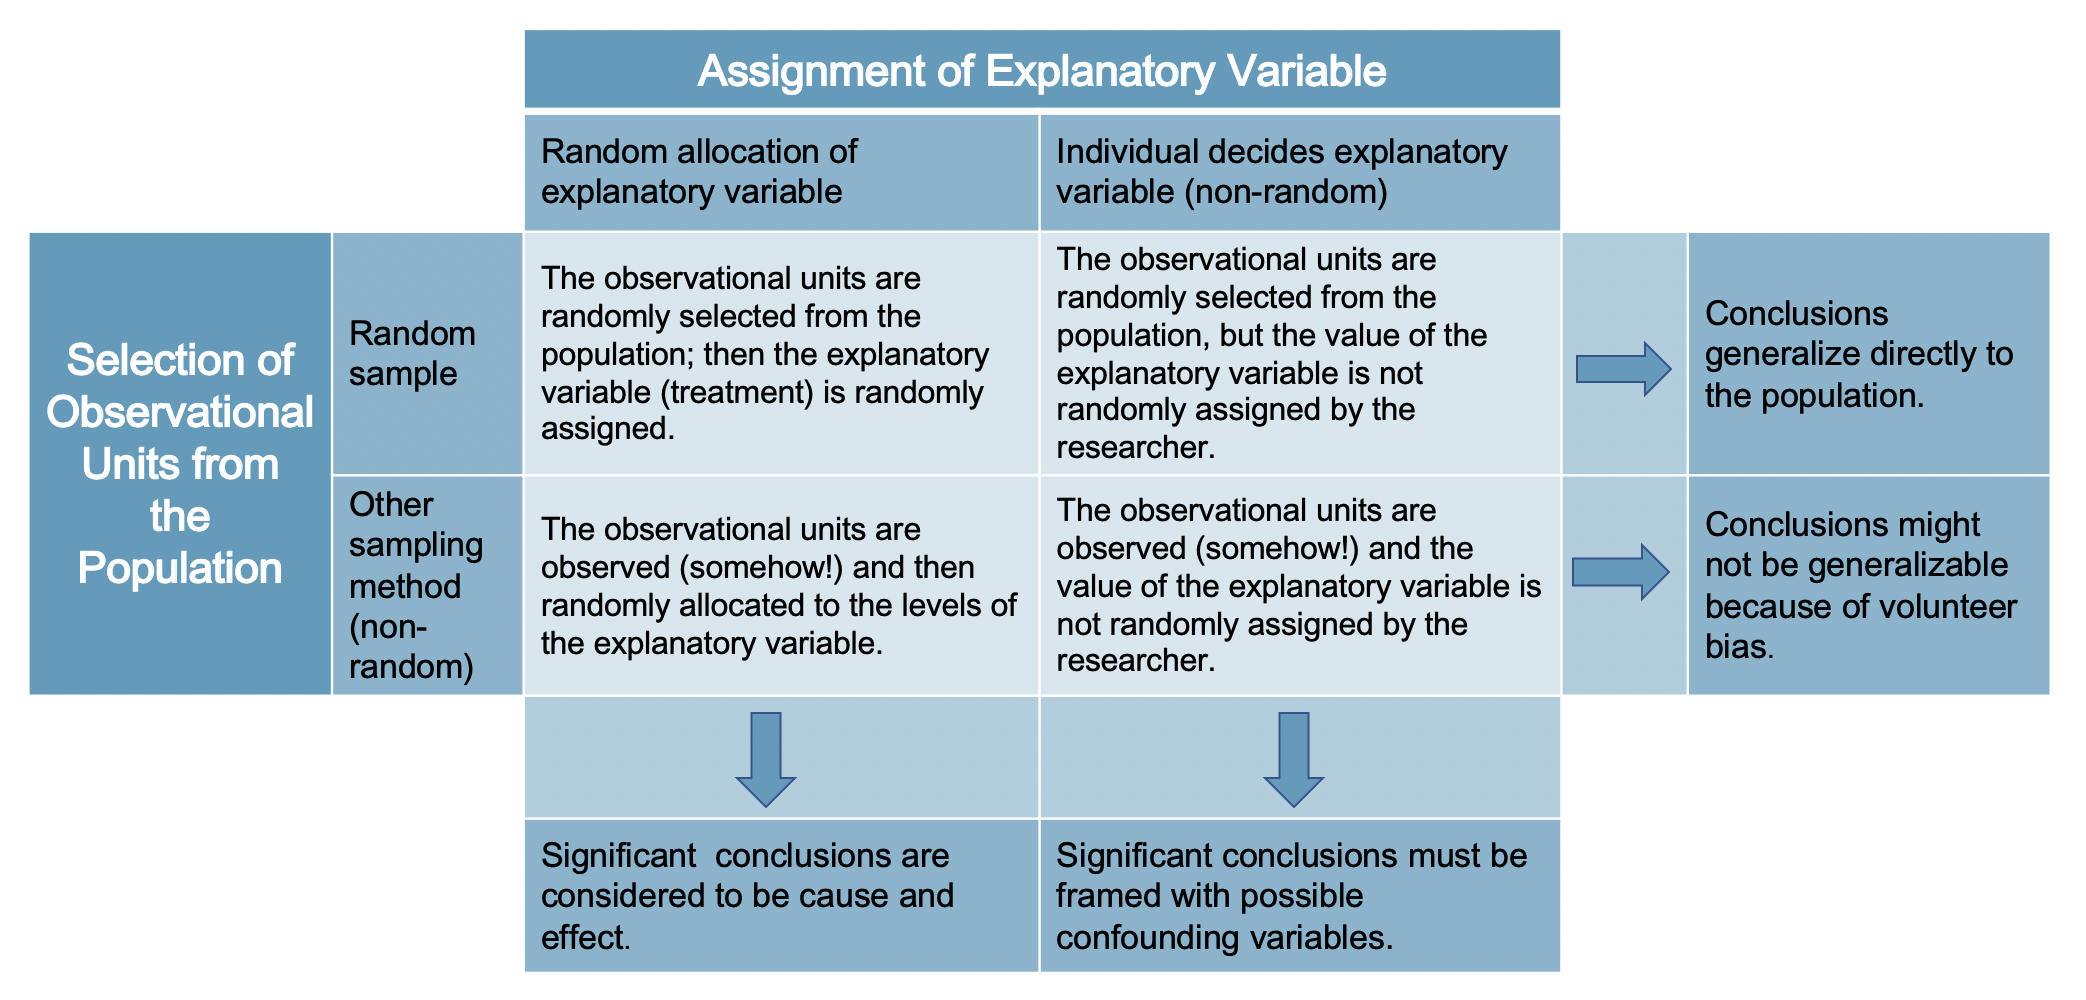
\includegraphics[width=1\linewidth]{images/randsampValloc} 

}

\caption{As we will see, analysis conclusions should be made carefully according to how the data were collected.  Note that very few datasets come from the top left box because usually ethics require that randomly allocated treatments can only be given to volunteers. Both representative (ideally random) sampling and experiments (random allocation) are important for how statistical conclusions can be made on populations.}\label{fig:randsampValloc}
\end{figure}

\hypertarget{terms-1}{%
\subsection{Terms}\label{terms-1}}

We introduced the following terms in the chapter.
If you're not sure what some of these terms mean, we recommend you go back in the text and review their definitions.
We are purposefully presenting them in alphabetical order, instead of in order of appearance, so they will be a little more challenging to locate.
However you should be able to easily spot them as \textbf{bolded text}.

\begin{tabu} to \linewidth {>{\raggedright}X>{\raggedright}X>{\raggedright}X}
\toprule
\cellcolor{gray!6}{anecdotal evidence} & \cellcolor{gray!6}{multistage sample} & \cellcolor{gray!6}{replication crisis}\\
bias & non-response bias & representative\\
\cellcolor{gray!6}{blind} & \cellcolor{gray!6}{non-response rate} & \cellcolor{gray!6}{retrospective study}\\
blocking & observational data & sample\\
\cellcolor{gray!6}{cluster} & \cellcolor{gray!6}{parameter} & \cellcolor{gray!6}{sample bias}\\
\addlinespace
cluster sampling & placebo & simple random sample\\
\cellcolor{gray!6}{confounding variable} & \cellcolor{gray!6}{placebo effect} & \cellcolor{gray!6}{simple random sampling}\\
control & population & statistic\\
\cellcolor{gray!6}{control group} & \cellcolor{gray!6}{prospective study} & \cellcolor{gray!6}{strata}\\
convenience sample & pseudoreplication & stratified sampling\\
\addlinespace
\cellcolor{gray!6}{double-blind} & \cellcolor{gray!6}{randomized experiment} & \cellcolor{gray!6}{treatment group}\\
experiment & replicatation & \\
\bottomrule
\end{tabu}

\hypertarget{chp2-exercises}{%
\section{Exercises}\label{chp2-exercises}}

\begin{enumerate}
\def\labelenumi{\arabic{enumi}.}
\item
  \textbf{Parameters and statistics.}
  Identify which value represents the sample mean and which value represents the claimed population mean.

  \begin{enumerate}
  \def\labelenumii{\alph{enumii}.}
  \item
    American households spent an average of about \$52 in 2007 on Halloween merchandise such as costumes, decorations and candy. To see if this number had changed, researchers conducted a new survey in 2008 before industry numbers were reported. The survey included 1,500 households and found that average Halloween spending was \$58 per household.
  \item
    The average GPA of students in 2001 at a private university was 3.37. A survey on a sample of 203 students from this university yielded an average GPA of 3.59 a decade later.
  \end{enumerate}
\item
  \textbf{Sleeping in college.}
  A recent article in a college newspaper stated that college students get an average of 5.5 hrs of sleep each night.
  A student who was skeptical about this value decided to conduct a survey by randomly sampling 25 students.
  On average, the sampled students slept 6.25 hours per night.
  Identify which value represents the sample mean and which value represents the claimed population mean.
\item
  \textbf{Air pollution and birth outcomes, scope of inference.}
  Researchers collected data to examine the relationship between air pollutants and preterm births in Southern California.
  During the study air pollution levels were measured by air quality monitoring stations.
  Length of gestation data were collected on 143,196 births between the years 1989 and 1993, and air pollution exposure during gestation was calculated for each birth. \citep{Ritz+Yu+Chapa+Fruin:2000}

  \begin{enumerate}
  \def\labelenumii{\alph{enumii}.}
  \item
    Identify the population of interest and the sample in this study.
  \item
    Comment on whether or not the results of the study can be generalized to the population, and if the findings of the study can be used to establish causal relationships.
  \end{enumerate}
\item
  \textbf{Cheaters, scope of inference.}
  Researchers studying the relationship between honesty, age and self-control conducted an experiment on 160 children between the ages of 5 and 15.
  The researchers asked each child to toss a fair coin in private and to record the outcome (white or black) on a paper sheet, and said they would only reward children who report white.
  Half the students were explicitly told not to cheat and the others were not given any explicit instructions. Differences were observed in the cheating rates in the instruction and no instruction groups, as well as some differences across children's characteristics within each group. \citep{Bucciol:2011}

  \begin{enumerate}
  \def\labelenumii{\alph{enumii}.}
  \item
    Identify the population of interest and the sample in this study.
  \item
    Comment on whether or not the results of the study can be generalized to the population, and if the findings of the study can be used to establish causal relationships.
  \end{enumerate}
\item
  \textbf{Gamification and statistics, scope of inference.}
  Researchers investigating the effects of gamification (application of game-design elements and game principles in non-game contexts) on learning statistics randomly assigned 365 college students in a statistics course to one of four groups; one of these groups had no reading exercises and no gamification, one group had reading but no gamification, one group had gamification but no reading, and a final group had gamification and reading.
  Students in all groups also attended lectures.
  The study found that gamification had a positive impact on student learning compared to traditional teaching methods involving reading exercises.@Legaki:2020{]}

  \begin{enumerate}
  \def\labelenumii{\alph{enumii}.}
  \item
    Identify the population of interest and the sample in this study.
  \item
    Comment on whether or not the results of the study can be generalized to the population, and if the findbngs of the study can be used to establish causal relationships.
  \end{enumerate}
\item
  \textbf{Stealers, scope of inference.}
  In a study of the relationship between socio-economic class and unethical behavior, 129 University of California undergraduates at Berkeley were asked to identify themselves as having low or high social-class by comparing themselves to others with the most (least) money, most (least) education, and most (least) respected jobs.
  They were also presented with a jar of individually wrapped candies and informed that the candies were for children in a nearby laboratory, but that they could take some if they wanted.
  After completing some unrelated tasks, participants reported the number of candies they had taken.
  It was found that those who were identified as upper-class took more candy than others. \citep{Piff:2012}

  \begin{enumerate}
  \def\labelenumii{\alph{enumii}.}
  \item
    Identify the population of interest and the sample in this study.
  \item
    Comment on whether or not the results of the study can be generalized to the population, and if the findings of the study can be used to establish causal relationships.
  \end{enumerate}
\item
  \textbf{Relaxing after work.}
  The General Social Survey asked the question, \emph{``After an average work day, about how many hours do you have to relax or pursue activities that you enjoy?''} to a random sample of 1,155 Americans.
  The average relaxing time was found to be 1.65 hours.
  Determine which of the following is an observation, a variable, a sample statistic (value calculated based on the observed sample), or a population parameter.\footnote{The data used in this exercise comes from the \href{https://www.openintro.org/go?id=textbook-gss-data\&referrer=ims0_html}{General Social Survey, 2018}.}

  \begin{enumerate}
  \def\labelenumii{\alph{enumii}.}
  \item
    An American in the sample.
  \item
    Number of hours spent relaxing after an average work day.
  \item
    1.65.
  \item
    Average number of hours all Americans spend relaxing after an average work day.
  \end{enumerate}
\item
  \textbf{Cats on YouTube.}
  Suppose you want to estimate the percentage of videos on YouTube that are cat videos.
  It is impossible for you to watch all videos on YouTube so you use a random video picker to select 1000 videos for you.
  You find that 2\% of these videos are cat videos.
  Determine which of the following is an observation, a variable, a sample statistic (value calculated based on the observed sample), or a population parameter.

  \begin{enumerate}
  \def\labelenumii{\alph{enumii}.}
  \item
    Percentage of all videos on YouTube that are cat videos.
  \item
    2\%.
  \item
    A video in your sample.
  \item
    Whether or not a video is a cat video.
  \end{enumerate}
\item
  \textbf{Course satisfaction across sections.}
  A large college class has 160 students.
  All 160 students attend the lectures together, but the students are divided into 4 groups, each of 40 students, for lab sections administered by different teaching assistants.
  The professor wants to conduct a survey about how satisfied the students are with the course, and he believes that the lab section a student is in might affect the student's overall satisfaction with the course.

  \begin{enumerate}
  \def\labelenumii{\alph{enumii}.}
  \item
    What type of study is this?
  \item
    Suggest a sampling strategy for carrying out this study.
  \end{enumerate}
\item
  \textbf{Housing proposal across dorms.}
  On a large college campus first-year students and sophomores live in dorms located on the eastern part of the campus and juniors and seniors live in dorms located on the western part of the campus.
  Suppose you want to collect student opinions on a new housing structure the college administration is proposing and you want to make sure your survey equally represents opinions from students from all years.

  \begin{enumerate}
  \def\labelenumii{\alph{enumii}.}
  \item
    What type of study is this?
  \item
    Suggest a sampling strategy for carrying out this study.
  \end{enumerate}
\item
  \textbf{Internet use and life expectancy.}
  The following scatterplot was created as part of a study evaluating the relationship between estimated life expectancy at birth (as of 2014) and percentage of internet users (as of 2009) in 208 countries for which such data were available.\footnote{The data used in this exercise can be found in the \textbf{openintro} R package: \href{http://openintrostat.github.io/openintro/reference/cia_factbook.html}{\texttt{cia\_factbook}}.}

  \begin{center}\includegraphics[width=0.9\linewidth]{02-data-design_files/figure-latex/unnamed-chunk-22-1} \end{center}

  \begin{enumerate}
  \def\labelenumii{\alph{enumii}.}
  \item
    Describe the relationship between life expectancy and percentage of internet users.
  \item
    What type of study is this?
  \item
    State a possible confounding variable that might explain this relationship and describe its potential effect.
  \end{enumerate}
\item
  \textbf{Stressed out.}
  A study that surveyed a random sample of otherwise healthy high school students found that they are more likely to get muscle cramps when they are stressed.
  The study also noted that students drink more coffee and sleep less when they are stressed.

  \begin{enumerate}
  \def\labelenumii{\alph{enumii}.}
  \item
    What type of study is this?
  \item
    Can this study be used to conclude a causal relationship between increased stress and muscle cramps?
  \item
    State possible confounding variables that might explain the observed relationship between increased stress and muscle cramps.
  \end{enumerate}
\item
  \textbf{Evaluate sampling methods.}
  A university wants to determine what fraction of its undergraduate student body support a new \$25 annual fee to improve the student union.
  For each proposed method below, indicate whether the method is reasonable or not.

  \begin{enumerate}
  \def\labelenumii{\alph{enumii}.}
  \item
    Survey a simple random sample of 500 students.
  \item
    Stratify students by their field of study, then sample 10\% of students from each stratum.
  \item
    Cluster students by their ages (e.g.~18 years old in one cluster, 19 years old in one cluster, etc.), then randomly sample three clusters and survey all students in those clusters.
  \end{enumerate}
\item
  \textbf{Random digit dialing.}
  The Gallup Poll uses a procedure called random digit dialing, which creates phone numbers based on a list of all area codes in America in conjunction with the associated number of residential households in each area code.
  Give a possible reason the Gallup Poll chooses to use random digit dialing instead of picking phone numbers from the phone book.
\item
  \textbf{Haters are gonna hate, study confirms.}
  A study published in the \emph{Journal of Personality and Social Psychology} asked a group of 200 randomly sampled participants recruited online using Amazon's Mechanical Turk to evaluate how they felt about various subjects, such as camping, health care, architecture, taxidermy, crossword puzzles, and Japan in order to measure their attitude towards mostly independent stimuli.
  Then, they presented the participants with information about a new product: a microwave oven.
  This microwave oven does not exist, but the participants didn't know this, and were given three positive and three negative fake reviews.
  People who reacted positively to the subjects on the dispositional attitude measurement also tended to react positively to the microwave oven, and those who reacted negatively tended to react negatively to it.
  Researchers concluded that \emph{``some people tend to like things, whereas others tend to dislike things, and a more thorough understanding of this tendency will lead to a more thorough understanding of the psychology of attitudes.''} \citep{Hepler:2013}

  \begin{enumerate}
  \def\labelenumii{\alph{enumii}.}
  \item
    What are the cases?
  \item
    What is (are) the response variable(s) in this study?
  \item
    What is (are) the explanatory variable(s) in this study?
  \item
    Does the study employ random sampling? Explain. How could they have obtained participants?
  \item
    Is this an observational study or an experiment? Explain your reasoning.
  \item
    Can we establish a causal link between the explanatory and response variables?
  \item
    Can the results of the study be generalized to the population at large?
  \end{enumerate}
\item
  \textbf{Family size.}
  Suppose we want to estimate household size, where a \emph{``household''} is defined as people living together in the same dwelling, and sharing living accommodations.
  If we select students at random at an elementary school and ask them what their family size is, will this be a good measure of household size?
  Or will our average be biased?
  If so, will it overestimate or underestimate the true value?
\item
  \textbf{Sampling strategies.}
  A statistics student who is curious about the relationship between the amount of time students spend on social networking sites and their performance at school decides to conduct a survey.
  Various research strategies for collecting data are described below. In each, name the sampling method proposed and any bias you might expect.

  \begin{enumerate}
  \def\labelenumii{\alph{enumii}.}
  \item
    They randomly sample 40 students from the study's population, give them the survey, ask them to fill it out and bring it back the next day.
  \item
    They give out the survey only to their friends, making sure each one of them fills out the survey.
  \item
    They post a link to an online survey on Facebook and ask their friends to fill out the survey.
  \item
    They randomly sample 5 classes and asks a random sample of students from those classes to fill out the survey.
  \end{enumerate}
\item
  \textbf{Reading the paper.}
  Below are excerpts from two articles published in the \emph{NY Times}:

  \begin{enumerate}
  \def\labelenumii{\alph{enumii}.}
  \tightlist
  \item
    An excerpt from an article titled \emph{Risks: Smokers Found More Prone to Dementia} is below. Based on this study, can we conclude that smoking causes dementia later in life? Explain your reasoning. \citep{news:smokingDementia}
  \end{enumerate}

  \begin{quote}
  ``Researchers analyzed data from 23,123 health plan members who participated in a voluntary exam and health behavior survey from 1978 to 1985, when they were 50-60 years old. 23 years later, about 25\% of the group had dementia, including 1,136 with Alzheimer's disease and 416 with vascular dementia. After adjusting for other factors, the researchers concluded that pack-a-day smokers were 37\% more likely than nonsmokers to develop dementia, and the risks went up with increased smoking; 44\% for one to two packs a day; and twice the risk for more than two packs.''
  \end{quote}

  \begin{enumerate}
  \def\labelenumii{\alph{enumii}.}
  \setcounter{enumii}{1}
  \tightlist
  \item
    An excerpt from an article titled \emph{The School Bully Is Sleepy} is below. A friend of yours who read the article says, \emph{``The study shows that sleep disorders lead to bullying in school children.''} Is this statement justified? If not, how best can you describe the conclusion that can be drawn from this study? \citep{news:bullySleep}
  \end{enumerate}

  \begin{quote}
  ``The University of Michigan study, collected survey data from parents on each child's sleep habits and asked both parents and teachers to assess behavioral concerns. About a third of the students studied were identified by parents or teachers as having problems with disruptive behavior or bullying. The researchers found that children who had behavioral issues and those who were identified as bullies were twice as likely to have shown symptoms of sleep disorders.''
  \end{quote}
\item
  \textbf{Light and exam performance.}
  A study is designed to test the effect of light level on exam performance of students.
  The researcher believes that light levels might have different effects on people who wear glasses and people who don't, so they want to make sure both groups of people are equally represented in each treatment.
  The treatments are fluorescent overhead lighting, yellow overhead lighting, no overhead lighting (only desk lamps).

  \begin{enumerate}
  \def\labelenumii{\alph{enumii}.}
  \item
    What is the response variable?
  \item
    What is the explanatory variable? What are its levels?
  \item
    What is the blocking variable? What are its levels?
  \end{enumerate}
\item
  \textbf{Vitamin supplements.}
  To assess the effectiveness of taking large doses of vitamin C in reducing the duration of the common cold, researchers recruited 400 healthy volunteers from staff and students at a university.
  A~quarter of the patients were assigned a placebo, and the rest were evenly divided between 1g Vitamin C, 3g Vitamin C, or 3g Vitamin C plus additives to be taken at onset of a cold for the following two days.
  All tablets had identical appearance and packaging.
  The nurses who handed the prescribed pills to the patients knew which patient received which treatment, but the researchers assessing the patients when they were sick did not.
  No significant differences were observed in any measure of cold duration or severity between the four groups, and the placebo group had the shortest duration of symptoms. \citep{Audera:2001}

  \begin{enumerate}
  \def\labelenumii{\alph{enumii}.}
  \item
    Was this an experiment or an observational study? Why?
  \item
    What are the explanatory and response variables in this study?
  \item
    Were the patients blinded to their treatment?
  \item
    Was this study double-blind?
  \item
    Participants are ultimately able to choose whether or not to use the pills prescribed to them. We might expect that not all of them will adhere and take their pills. Does this introduce a confounding variable to the study? Explain your reasoning.
  \end{enumerate}
\item
  \textbf{Light, noise, and exam performance.}
  A study is designed to test the effect of light level and noise level on exam performance of students.
  The researcher believes that light and noise levels might have different effects on people who wear glasses and people who don't, so they want to make sure both groups of people are equally represented in each treatment.
  The light treatments considered are fluorescent overhead lighting, yellow overhead lighting, no overhead lighting (only desk lamps).
  The noise treatments considered are no noise, construction noise, and human chatter noise.

  \begin{enumerate}
  \def\labelenumii{\arabic{enumii}.}
  \item
    What type of study is this?
  \item
    How many factors are considered in this study? Identify them, and describe their levels.
  \item
    What is the role of the wearing glasses variable in this study?
  \end{enumerate}
\item
  \textbf{Music and learning.}
  You would like to conduct an experiment in class to see if students learn better if they study without any music, with music that has no lyrics (instrumental), or with music that has lyrics.
  Briefly outline a design for this study.
\item
  \textbf{Soda preference.}
  You would like to conduct an experiment in class to see if your classmates prefer the taste of regular Coke or Diet Coke.
  Briefly outline a design for this study.
\item
  \textbf{Exercise and mental health.}
  A researcher is interested in the effects of exercise on mental health and they propose the following study: use stratified random sampling to ensure representative proportions of 18-30, 31-40 and 41- 55 year olds from the population.
  Next, randomly assign half the subjects from each age group to exercise twice a week, and instruct the rest not to exercise.
  Conduct a mental health exam at the beginning and at the end of the study, and compare the results.

  \begin{enumerate}
  \def\labelenumii{\alph{enumii}.}
  \item
    What type of study is this?
  \item
    What are the treatment and control groups in this study?
  \item
    Does this study make use of blocking? If so, what is the blocking variable?
  \item
    Does this study make use of blinding?
  \item
    Comment on whether or not the results of the study can be used to establish a causal relationship between exercise and mental health, and indicate whether or not the conclusions can be generalized to the population at large.
  \item
    Suppose you are given the task of determining if this proposed study should get funding. Would you have any reservations about the study proposal?
  \end{enumerate}
\item
  \textbf{Chia seeds and weight loss.}
  Chia Pets -- those terra-cotta figurines that sprout fuzzy green hair -- made the chia plant a household name. But chia has gained an entirely new reputation as a diet supplement.
  In one 2009 study, a team of researchers recruited 38 men and divided them randomly into two groups: treatment or control.
  They also recruited 38 women, and they randomly placed half of these participants into the treatment group and the other half into the control group.
  One group was given 25 grams of chia seeds twice a day, and the other was given a placebo.
  The subjects volunteered to be a part of the study.
  After 12 weeks, the scientists found no significant difference between the groups in appetite or weight loss. \citep{Nieman:2009}

  \begin{enumerate}
  \def\labelenumii{\alph{enumii}.}
  \item
    What type of study is this?
  \item
    What are the experimental and control treatments in this study?
  \item
    Has blocking been used in this study? If so, what is the blocking variable?
  \item
    Has blinding been used in this study?
  \item
    Comment on whether or not we can make a causal statement, and indicate whether or not we can generalize the conclusion to the population at large.
  \end{enumerate}
\item
  \textbf{City council survey.}
  A city council has requested a household survey be conducted in a suburban area of their city.
  The area is broken into many distinct and unique neighborhoods, some including large homes, some with only apartments, and others a diverse mixture of housing structures.
  For each part below, identify the sampling methods described, and describe the statistical pros and cons of the method in the city's context.

  \begin{enumerate}
  \def\labelenumii{\alph{enumii}.}
  \item
    Randomly sample 200 households from the city.
  \item
    Divide the city into 20 neighborhoods, and sample 10 households from each neighborhood.
  \item
    Divide the city into 20 neighborhoods, randomly sample 3 neighborhoods, and then sample all households from those 3 neighborhoods.
  \item
    Divide the city into 20 neighborhoods, randomly sample 8 neighborhoods, and then randomly sample 50 households from those neighborhoods.
  \item
    Sample the 200 households closest to the city council offices.
  \end{enumerate}
\item
  \textbf{Flawed reasoning.}
  Identify the flaw(s) in reasoning in the following scenarios.
  Explain what the individuals in the study should have done differently if they wanted to make such strong conclusions.

  \begin{enumerate}
  \def\labelenumii{\alph{enumii}.}
  \item
    Students at an elementary school are given a questionnaire that they are asked to return after their parents have completed it. One of the questions asked is, \emph{``Do you find that your work schedule makes it difficult for you to spend time with your kids after school?''} Of the parents who replied, 85\% said \emph{``no''}. Based on these results, the school officials conclude that a great majority of the parents have no difficulty spending time with their kids after school.
  \item
    A survey is conducted on a simple random sample of 1,000 women who recently gave birth, asking them about whether or not they smoked during pregnancy. A follow-up survey asking if the children have respiratory problems is conducted 3 years later. However, only 567 of these women are reached at the same address. The researcher reports that these 567 women are representative of all mothers.
  \item
    An orthopedist administers a questionnaire to 30 of his patients who do not have any joint problems and finds that 20 of them regularly go running. He concludes that running decreases the risk of joint problems.
  \end{enumerate}
\item
  \textbf{Income and education in US counties.}
  The scatterplot below shows the relationship between per capita income (in thousands of dollars) and percent of population with a bachelor's degree in 3,142 counties in the US in 2019.\footnote{The data used in this exercise can be found in the \textbf{openintro} R package: \href{http://openintrostat.github.io/openintro/reference/county_complete.html}{\texttt{county\_complete}}.}

  \begin{center}\includegraphics[width=0.9\linewidth]{02-data-design_files/figure-latex/unnamed-chunk-23-1} \end{center}

  \begin{enumerate}
  \def\labelenumii{\alph{enumii}.}
  \item
    What are the explanatory and response variables?
  \item
    Describe the relationship between the two variables. Make sure to discuss unusual observations, if any.
  \item
    Can we conclude that having a bachelor's degree increases one's income?
  \end{enumerate}
\item
  \textbf{Eat well, feel better.}
  In a public health study on the effects of consumption of fruits and vegetables on psychological well-being in young adults, participants were randomly assigned to three groups: (1) diet-as-usual, (2) an ecological momentary intervention involving text message reminders to increase their fruits and vegetable consumption plus a voucher to purchase them, or (3) a fruit and vegetable intervention in which participants were given two additional daily servings of fresh fruits and vegetables to consume on top of their normal diet.
  Participants were asked to take a nightly survey on their smartphones.
  Participants were student volunteers at the University of Otago, New Zealand.
  At the end of the 14-day study, only participants in the third group showed improvements to their psychological well-being across the 14-days relative to the other groups. \citep{conner2017let}

  \begin{enumerate}
  \def\labelenumii{\alph{enumii}.}
  \item
    What type of study is this?
  \item
    Identify the explanatory and response variables.
  \item
    Comment on whether the results of the study can be generalized to the population.
  \item
    Comment on whether the results of the study can be used to establish causal relationships.
  \item
    A newspaper article reporting on the study states, ``The results of this study provide proof that giving young adults fresh fruits and vegetables to eat can have psychological benefits, even over a brief period of time.'' How would you suggest revising this statement so that it can be supported by the study?
  \end{enumerate}
\item
  \textbf{Screens, teens, and psychological well-being.}
  In a study of three nationally representative large-scale data sets from Ireland, the United States, and the United Kingdom (n = 17,247), teenagers between the ages of 12 to 15 were asked to keep a diary of their screen time and answer questions about how they felt or acted.
  The answers to these questions were then used to compute a psychological well-being score.
  Additional data were collected and included in the analysis, such as each child's sex and age, and on the mother's education, ethnicity, psychological distress, and employment.
  The study concluded that there is little clear-cut evidence that screen time decreases adolescent well-being. \citep{orben2018screens}

  \begin{enumerate}
  \def\labelenumii{\alph{enumii}.}
  \item
    What type of study is this?
  \item
    Identify the explanatory variables.
  \item
    Identify the response variable.
  \item
    Comment on whether the results of the study can be generalized to the population, and why.
  \item
    Comment on whether the results of the study can be used to establish causal relationships.
  \end{enumerate}
\end{enumerate}

\hypertarget{data-applications}{%
\chapter{Applications: Data}\label{data-applications}}

\hypertarget{case-study-passwords}{%
\section{Case study: Passwords}\label{case-study-passwords}}

Stop for a second and think about how many passwords you've used so far today.
You've probably used one to unlock your phone, one to check email, and probably at least one to log on to a social media account.
Made a debit purchase?
You've probably entered a password there too.

If you're reading this book, and particularly if you're reading it online, chances are you have had to create a password once or twice in your life.
And if you are diligent about your safety and privacy, you've probably chosen passwords that would be hard for others to guess, or \emph{crack}.

In this case study we introduce a dataset on passwords.
The goal of the case study is to walk you through what a data scientist does when they first get a hold of a dataset as well as to provide some ``foreshadowing'' of concepts and techniques we'll introduce in the next few chapters on exploratory data analysis.

\begin{data}
The data can be found in the \href{https://thebioengineer.github.io/tidytuesdayR/}{tidytuesdayR} package: \href{https://github.com/rfordatascience/tidytuesday/blob/master/data/2020/2020-01-14/readme.md}{\texttt{passwords}}.

\end{data}

Table \ref{tab:passwords-df-head} shows the first ten rows from the dataset, which are the ten most common passwords.
Perhaps unsurprisingly, ``password'' tops the list, followed by ``123456''.

\begin{table}

\caption{\label{tab:passwords-df-head}Top ten rows of the `passwords` dataset.}
\centering
\begin{tabular}[t]{r|l|l|r|l|r|r}
\hline
rank & password & category & value & time\_unit & offline\_crack\_sec & strength\\
\hline
\cellcolor{gray!6}{1} & \cellcolor{gray!6}{password} & \cellcolor{gray!6}{password-related} & \cellcolor{gray!6}{6.91} & \cellcolor{gray!6}{years} & \cellcolor{gray!6}{2.170} & \cellcolor{gray!6}{8}\\
\hline
2 & 123456 & simple-alphanumeric & 18.52 & minutes & 0.000 & 4\\
\hline
\cellcolor{gray!6}{3} & \cellcolor{gray!6}{12345678} & \cellcolor{gray!6}{simple-alphanumeric} & \cellcolor{gray!6}{1.29} & \cellcolor{gray!6}{days} & \cellcolor{gray!6}{0.001} & \cellcolor{gray!6}{4}\\
\hline
4 & 1234 & simple-alphanumeric & 11.11 & seconds & 0.000 & 4\\
\hline
\cellcolor{gray!6}{5} & \cellcolor{gray!6}{qwerty} & \cellcolor{gray!6}{simple-alphanumeric} & \cellcolor{gray!6}{3.72} & \cellcolor{gray!6}{days} & \cellcolor{gray!6}{0.003} & \cellcolor{gray!6}{8}\\
\hline
6 & 12345 & simple-alphanumeric & 1.85 & minutes & 0.000 & 4\\
\hline
\cellcolor{gray!6}{7} & \cellcolor{gray!6}{dragon} & \cellcolor{gray!6}{animal} & \cellcolor{gray!6}{3.72} & \cellcolor{gray!6}{days} & \cellcolor{gray!6}{0.003} & \cellcolor{gray!6}{8}\\
\hline
8 & baseball & sport & 6.91 & years & 2.170 & 4\\
\hline
\cellcolor{gray!6}{9} & \cellcolor{gray!6}{football} & \cellcolor{gray!6}{sport} & \cellcolor{gray!6}{6.91} & \cellcolor{gray!6}{years} & \cellcolor{gray!6}{2.170} & \cellcolor{gray!6}{7}\\
\hline
10 & letmein & password-related & 3.19 & months & 0.084 & 8\\
\hline
\end{tabular}
\end{table}

When you encounter a new dataset, taking a peek at the first few rows we we did in Table \ref{tab:passwords-df-head} is almost instinctual.
It can often be helpful to take a look at the last few rows of the data as well to get a sense of the size of the data as well as potentially discover any characteristics that may not be apparent in the top few rows.
Table \ref{tab:passwords-df-tail} shows the bottom ten rows of the passwords dataset, which reveals that we are looking at a dataset of 500 passwords.

\begin{table}

\caption{\label{tab:passwords-df-tail}Bottom ten rows of the `passwords` dataset.}
\centering
\begin{tabular}[t]{r|l|l|r|l|r|r}
\hline
rank & password & category & value & time\_unit & offline\_crack\_sec & strength\\
\hline
\cellcolor{gray!6}{491} & \cellcolor{gray!6}{natasha} & \cellcolor{gray!6}{name} & \cellcolor{gray!6}{3.19} & \cellcolor{gray!6}{months} & \cellcolor{gray!6}{0.084} & \cellcolor{gray!6}{7}\\
\hline
492 & sniper & cool-macho & 3.72 & days & 0.003 & 8\\
\hline
\cellcolor{gray!6}{493} & \cellcolor{gray!6}{chance} & \cellcolor{gray!6}{name} & \cellcolor{gray!6}{3.72} & \cellcolor{gray!6}{days} & \cellcolor{gray!6}{0.003} & \cellcolor{gray!6}{7}\\
\hline
494 & genesis & nerdy-pop & 3.19 & months & 0.084 & 7\\
\hline
\cellcolor{gray!6}{495} & \cellcolor{gray!6}{hotrod} & \cellcolor{gray!6}{cool-macho} & \cellcolor{gray!6}{3.72} & \cellcolor{gray!6}{days} & \cellcolor{gray!6}{0.003} & \cellcolor{gray!6}{7}\\
\hline
496 & reddog & cool-macho & 3.72 & days & 0.003 & 6\\
\hline
\cellcolor{gray!6}{497} & \cellcolor{gray!6}{alexande} & \cellcolor{gray!6}{name} & \cellcolor{gray!6}{6.91} & \cellcolor{gray!6}{years} & \cellcolor{gray!6}{2.170} & \cellcolor{gray!6}{9}\\
\hline
498 & college & nerdy-pop & 3.19 & months & 0.084 & 7\\
\hline
\cellcolor{gray!6}{499} & \cellcolor{gray!6}{jester} & \cellcolor{gray!6}{name} & \cellcolor{gray!6}{3.72} & \cellcolor{gray!6}{days} & \cellcolor{gray!6}{0.003} & \cellcolor{gray!6}{7}\\
\hline
500 & passw0rd & password-related & 92.27 & years & 29.020 & 28\\
\hline
\end{tabular}
\end{table}

At this stage it's also useful to think about how these data were collected, as that will inform the scope of any inference you can make based on your analysis of the data.

\begin{guidedpractice}
Do these data come from an observational study or an experiment?\footnote{This is an observational study.
  Researchers collected data on existing passwords in use and identified most common ones to put together this dataset.}

\end{guidedpractice}

\begin{guidedpractice}
There are 500 rows and 7 in the dataset.
What does each row and each column represent?\footnote{Each row represents a password and each column represents a variable which contains information on each password.}

\end{guidedpractice}

Once you've identified the rows and columns, it's useful to review the data dictionary to learn about what each column in the dataset represents.
This is provided in Table \ref{tab:passwords-var-def}.

\begin{table}

\caption{\label{tab:passwords-var-def}Variables and their descriptions for the `passwords` data set.}
\centering
\begin{tabular}[t]{l|l}
\hline
variable & description\\
\hline
\cellcolor{gray!6}{\ttfamily{rank}} & \cellcolor{gray!6}{Popularity in the database of released passwords.}\\
\hline
\ttfamily{password} & Actual text of the password.\\
\hline
\cellcolor{gray!6}{\ttfamily{category}} & \cellcolor{gray!6}{Category password falls into.}\\
\hline
\ttfamily{value} & Time to crack by online guessing.\\
\hline
\cellcolor{gray!6}{\ttfamily{time\_unit}} & \cellcolor{gray!6}{Time unit to match with value.}\\
\hline
\ttfamily{offline\_crack\_sec} & Time to crack offline in seconds.\\
\hline
\cellcolor{gray!6}{\ttfamily{strength}} & \cellcolor{gray!6}{Strength of password, relative to only to passwords in this dataset. Lower values indicate weaker passwords.}\\
\hline
\end{tabular}
\end{table}

We now have a better sense of what each column represents, but we don't yet know much about the characteristics of each of the variables.

\begin{workedexample}
Determine whether each variable in the passwords dataset is numerical or categorical.
For numerical variables, further classify them as continuous or discrete.
For categorical variables, determine if the variable is ordinal.

\begin{center}\rule{0.5\linewidth}{0.5pt}\end{center}

The numerical variables in the dataset are \texttt{rank} (discrete), \texttt{value} (continuous), and \texttt{offline\_crack\_sec} (continuous).
The categorical variables are \texttt{password}, \texttt{time\_unit}.
The strength variable is trickier to classify -- we can think of it as discrete numerical or as an ordinal variable as it takes on numerical values, however it's used to categorize the passwords on an ordinal scale.
One way of approaching this is thinking about whether the values the variable takes vary linearly, e.g.~is the difference in strength between passwords with strength levels 8 and 9 the same as the difference with those with strength levels 9 and 10.
If this is not necessarily the case, we would classify the variable as ordinal.
Determining the classification of this variable requires understanding how \texttt{strength} values were determined, which is a very typical workflow for working with data.
Sometimes the data dictionary (presented in Table \ref{tab:passwords-var-def} isn't sufficient, and we need to go back to the data source and try to understand the data better before we can proceed with the analysis meaningfully.

\end{workedexample}

Next, let's try to get to know each variable a little bit better.
For categorical variables, this involves figuring out what their levels are and how commonly represented they are in the data.
Figure \ref{fig:passwords-cat} shows the distributions of the categorical variables in this dataset.
We can see that password strengths of 0-10 are more common than higher values.
The most common password category is name (e.g.~michael, jennifer, jordan, etc.) and the least common is food (e.g.~pepper, cheese, coffee, etc.).
Many passwords can be cracked in the matter of days by online cracking with some taking as little as seconds and some as long as years to break.
Each of these visualizations is a bar plot, which you will learn more about in Chapter \ref{explore-categorical}.

\begin{figure}

{\centering \includegraphics[width=1\linewidth]{03-data-applications_files/figure-latex/passwords-cat-1} 

}

\caption{Distributions of the categorical variables in the `passwords` dataset. Plot A shows the distribution of password strengths, Plot B password categories, and Plot C length of time it takes to crack the passwords by online guessing.}\label{fig:passwords-cat}
\end{figure}

Similarly, we can examine the distributions of the numerical variables as well.
We already know that rank ranges between 1 and 500 in this dataset, based on Table \ref{tab:passwords-df-head} and Table \ref{tab:passwords-df-tail}.
The value variable is slightly more complicated to consider since the numerical values in that column are meaningless without the time unit that accompanies them.
Table \ref{tab:passwords-online-crack-summary} shows the minimum and maximum amount of time it takes to crack a password by online guessing.
For example there are 11 passwords in the dataset that can be broken in a matter of seconds, and each of them take 11.11 seconds to break, since the minimum and the maximum of observations in this group are exactly equal to this value.
And there are 65 passwords that take years to break, ranging from 2.56 years to 92.27 years.

\begin{table}

\caption{\label{tab:passwords-online-crack-summary}Minimum and maximum amount of time it takes to crack a password by online guessing as well as the number of observations that fall into each time unit category.}
\centering
\begin{tabular}[t]{l|r|r|r}
\hline
time\_unit & n & min & max\\
\hline
\cellcolor{gray!6}{seconds} & \cellcolor{gray!6}{11} & \cellcolor{gray!6}{11.11} & \cellcolor{gray!6}{11.11}\\
\hline
minutes & 51 & 1.85 & 18.52\\
\hline
\cellcolor{gray!6}{hours} & \cellcolor{gray!6}{43} & \cellcolor{gray!6}{3.09} & \cellcolor{gray!6}{17.28}\\
\hline
days & 238 & 1.29 & 3.72\\
\hline
\cellcolor{gray!6}{weeks} & \cellcolor{gray!6}{5} & \cellcolor{gray!6}{1.84} & \cellcolor{gray!6}{3.70}\\
\hline
months & 87 & 3.19 & 3.19\\
\hline
\cellcolor{gray!6}{years} & \cellcolor{gray!6}{65} & \cellcolor{gray!6}{2.56} & \cellcolor{gray!6}{92.27}\\
\hline
\end{tabular}
\end{table}

Even though passwords that take a large number of years to crack can seem like good options (see Table \ref{tab:passwords-long-crack} for a list of them), now that you've seen them here (and the fact that they are in a dataset of 500 most common passwords), you should not use them as secure passwords!

\begin{table}

\caption{\label{tab:passwords-long-crack}Passwords that take the longest amount of time to crack by online guessing.}
\centering
\begin{tabular}[t]{r|l|l|r|l|r|r}
\hline
rank & password & category & value & time\_unit & offline\_crack\_sec & strength\\
\hline
\cellcolor{gray!6}{26} & \cellcolor{gray!6}{trustno1} & \cellcolor{gray!6}{simple-alphanumeric} & \cellcolor{gray!6}{92.3} & \cellcolor{gray!6}{years} & \cellcolor{gray!6}{29.0} & \cellcolor{gray!6}{25}\\
\hline
336 & rush2112 & nerdy-pop & 92.3 & years & 29.0 & 48\\
\hline
\cellcolor{gray!6}{406} & \cellcolor{gray!6}{jordan23} & \cellcolor{gray!6}{sport} & \cellcolor{gray!6}{92.3} & \cellcolor{gray!6}{years} & \cellcolor{gray!6}{29.3} & \cellcolor{gray!6}{34}\\
\hline
500 & passw0rd & password-related & 92.3 & years & 29.0 & 28\\
\hline
\end{tabular}
\end{table}

The last numerical variable in the dataset is \texttt{offline\_crack\_sec}.
Figure \ref{fig:password-offline-crack-hist} shows the distribution of this variable, which reveals that all of these passwords can be cracked offline in under 30 seconds, with a large number of them being crackable in just a few seconds.

\begin{figure}

{\centering \includegraphics[width=0.9\linewidth]{03-data-applications_files/figure-latex/password-offline-crack-hist-1} 

}

\caption{Histogram of the length of time it takes to crack passwords offline.}\label{fig:password-offline-crack-hist}
\end{figure}

So far we examined the distributions of each individual variable, but it would be more interesting to explore relationships between multiple variables.
Figure \ref{fig:password-strength-rank-category} shows the relationship between rank and strength of passwords by category, where more common passwords (those with higher rank) are plotted higher on the y-axis than those that are less common in this dataset.
The stronger the password, the larger text it's represented with on the plot.
While this visualization reveals some passwords that are less common, and stronger than others, we should reiterate that you should not use any of these passwords.
And if you already do, it's time to go change it!

\begin{figure}

{\centering \includegraphics[width=1\linewidth]{03-data-applications_files/figure-latex/password-strength-rank-category-1} 

}

\caption{Rank vs. strength of 500 most common passwords by category.}\label{fig:password-strength-rank-category}
\end{figure}

In this case study, we introduced you to the very first steps a data scientist takes when they start working with a new dataset.
In the next few chapters we will introduce exploratory data analysis and you'll learn more about the various types of data visualizations and summary statistics you can make to get to know your data better.

Before you move on, we encourage you to think about whether the following questions can be answered with this dataset, and if yes, how you might go about answering them.
It's okay if your answer is ``I'm not sure'', we simply want to get your exploratory juices flowing to prime you for what's to come!

\begin{enumerate}
\def\labelenumi{\arabic{enumi}.}
\tightlist
\item
  What characteristics are associated with a strong vs.~a weak password?
\item
  Do more popular passwords take shorter or longer to crack compared to less popular passwords?
\item
  Are passwords that start with letters or numbers more common among the list of top 500 most common passwords?
\end{enumerate}

\hypertarget{data-tutorials}{%
\section{Interactive R tutorials}\label{data-tutorials}}

Navigate the concepts you've learned in this chapter in R using the following self-paced tutorials.
All you need is your browser to get started!

Update tutorial links

\href{https://openintrostat.github.io/ims-tutorials/01-getting-started-with-data/}{Tutorial 1: Getting Started with Data}

\href{https://openintro.shinyapps.io/ims-01-getting-started-with-data-01/}{Tutorial 1 - Lesson 1: Language of data}

\href{https://openintro.shinyapps.io/ims-01-getting-started-with-data-02/}{Tutorial 1 - Lesson 2: Types of studies}

\href{https://openintro.shinyapps.io/ims-01-getting-started-with-data-03/}{Tutorial 1 - Lesson 3: Sampling strategies and Experimental design}

\href{https://openintro.shinyapps.io/ims-01-getting-started-with-data-04/}{Tutorial 1 - Lesson 4: Case study}

You can also access the full list of tutorials supporting this book \href{https://openintrostat.github.io/ims-tutorials/}{here}.

\hypertarget{data-labs}{%
\section{R labs}\label{data-labs}}

Further apply the concepts you've learned in this chapter in R with computational labs that walk you through a data analysis case study.

\href{http://openintrostat.github.io/oilabs-tidy/01_intro_to_r/intro_to_r.html}{Intro to R - Birth rates}

\href{http://openintrostat.github.io/oilabs-tidy/}{Full list of labs supporting OpenIntro::Introduction to Modern Statistics}

\hypertarget{part-exploratory-data-analysis}{%
\part{Exploratory data analysis}\label{part-exploratory-data-analysis}}

\hypertarget{explore-categorical}{%
\chapter{Exploring categorical data}\label{explore-categorical}}

\begin{chapterintro}
This chapter focuses on exploring \textbf{categorical} data using summary statistics and visualizations.
The summaries and graphs presented in this chapter are created using statistical software; however, since this might be your first exposure to the concepts, we take our time in this chapter to detail how to create them.
Mastery of the content presented in this chapter will be crucial for understanding the methods and techniques introduced in rest of the book.

\end{chapterintro}

In this chapter we will work with data on loans from Lending Club that you've previously seen in Chapter \ref{data-hello}.
The \texttt{loan50} data set from Chapter \ref{data-hello} represents a sample from a larger loan data set called \texttt{loans}.
This larger data set contains information on 10,000 loans made through Lending Club.
We will examine the relationship between \texttt{homeownership}, which for the \texttt{loans} data can take a value of \texttt{rent}, \texttt{mortgage} (owns but has a mortgage), or \texttt{own}, and \texttt{app\_type}, which indicates whether the loan application was made with a partner or whether it was an individual application.

\begin{data}
The data can be found in the \href{http://openintrostat.github.io/openintro}{openintro} package: \href{http://openintrostat.github.io/openintro/reference/loans_full_schema.html}{loans}.

\end{data}

\hypertarget{contingency-tables-and-bar-plots}{%
\section{Contingency tables and bar plots}\label{contingency-tables-and-bar-plots}}

Table \ref{tab:loan-home-app-type-totals} summarizes two variables: \texttt{application\_type} and \texttt{homeownership}.
A table that summarizes data for two categorical variables in this way is called a \textbf{contingency table}.
Each value in the table represents the number of times a particular combination of variable outcomes occurred.
For example, the value 3496 corresponds to the number of loans in the data set where the borrower rents their home and the application type was by an individual.
Row and column totals are also included.
The \textbf{row totals} provide the total counts across each row and the \textbf{column totals} down each column.
We can also create a table that shows only the overall percentages or proportions for each combination of categories, or we can create a table for a single variable, such as the one shown in Table \ref{tab:loan-homeownership-totals} for the \texttt{homeownership} variable.

\begin{table}

\caption{\label{tab:loan-home-app-type-totals}A contingency table for application type and homeownership.}
\centering
\begin{tabular}[t]{l|r|r|r|r}
\hline
\multicolumn{1}{c|}{ } & \multicolumn{3}{c|}{homeownership} & \multicolumn{1}{c}{ } \\
\cline{2-4}
application\_type & mortgage & own & rent & Total\\
\hline
\cellcolor{gray!6}{joint} & \cellcolor{gray!6}{950} & \cellcolor{gray!6}{183} & \cellcolor{gray!6}{362} & \cellcolor{gray!6}{1495}\\
\hline
individual & 3839 & 1170 & 3496 & 8505\\
\hline
\cellcolor{gray!6}{Total} & \cellcolor{gray!6}{4789} & \cellcolor{gray!6}{1353} & \cellcolor{gray!6}{3858} & \cellcolor{gray!6}{10000}\\
\hline
\end{tabular}
\end{table}

\begin{table}

\caption{\label{tab:loan-homeownership-totals}A table summarizing the frequencies for each value of the homeownership variable: mortgage, own, and rent.}
\centering
\begin{tabular}[t]{l|r}
\hline
homeownership & Count\\
\hline
\cellcolor{gray!6}{mortgage} & \cellcolor{gray!6}{4789}\\
\hline
own & 1353\\
\hline
\cellcolor{gray!6}{rent} & \cellcolor{gray!6}{3858}\\
\hline
Total & 10000\\
\hline
\end{tabular}
\end{table}

A bar plot is a common way to display a single categorical variable.
The left panel of Figure \ref{fig:loan-homeownership-bar-plot} shows a \textbf{bar plot} for the \texttt{homeownership} variable.
In the right panel, the counts are converted into proportions, showing the proportion of observations that are in each level.

\begin{figure}

{\centering \includegraphics[width=0.9\linewidth]{04-explore-categorical_files/figure-latex/loan-homeownership-bar-plot-1} 

}

\caption{Two bar plots: the left panel shows the counts and the right panel shows the proportions of values of the homeownership variable.}\label{fig:loan-homeownership-bar-plot}
\end{figure}

\hypertarget{visualizing-two-categorical-variables}{%
\section{Visualizing two categorical variables}\label{visualizing-two-categorical-variables}}

\hypertarget{bar-plots-with-two-variables}{%
\subsection{Bar plots with two variables}\label{bar-plots-with-two-variables}}

We can display the distributions of two categorical variables on a bar plot concurrently.
Such plots are generally useful for visualizing the relationship between two categorical variables.
Figure \ref{fig:loan-homeownership-app-type-bar-plot} shows three such plots that visualize the relationship between \texttt{homeownership} and \texttt{application\_type} variables.
Plot A in Figure \ref{fig:loan-homeownership-app-type-bar-plot} is a \textbf{stacked bar plot}.
This plot most clearly displays that loan applicants most commonly live in mortgaged homes.
It is difficult to say, based on this plot alone, how different application types vary across the levels of homeownership.
Plot B is a \textbf{dodged bar plot}.
This plot most clearly displays that within each level of homeownership, individual applications are more common than joint applications.
Finally, plot C is a \textbf{standardized bar plot} (also known as \textbf{filled bar plot}).
This plot most clearly displays that joint applications are most common among applications who live in mortgaged homes, compared to renters and owners.
This type of visualization is helpful in understanding the fraction of individual or joint loan applications for borrowers in each level of \texttt{homeownership}.
Additionally, since the proportions of joint and individual loans vary across the groups, we can conclude that the two variables are associated for this sample.

\begin{figure}

{\centering \includegraphics[width=0.9\linewidth]{04-explore-categorical_files/figure-latex/loan-homeownership-app-type-bar-plot-1} 

}

\caption{Three bar plots (stacked, dodged, and standardized) displaying homeownership and application type variables.}\label{fig:loan-homeownership-app-type-bar-plot}
\end{figure}

\begin{workedexample}
Examine the three bar plots in Figure \ref{fig:loan-homeownership-app-type-bar-plot}.
When is the stacked, dodged, or standardized bar plot the most useful?

\begin{center}\rule{0.5\linewidth}{0.5pt}\end{center}

The stacked bar plot is most useful when it's reasonable to assign one variable as the explanatory variable (here \texttt{homeownership}) and the other variable as the response (here \texttt{application\_type}), since we are effectively grouping by one variable first and then breaking it down by the others.

Dodged bar plots are more agnostic in their display about which variable, if any, represents the explanatory and which the response variable.
It is also easy to discern the number of cases in of the six different group combinations.
However, one downside is that it tends to require more horizontal space; the narrowness of Plot B compared to the other two in Figure \ref{fig:loan-homeownership-app-type-bar-plot} makes the plot feel a bit cramped.
Additionally, when two groups are of very different sizes, as we see in the group \texttt{own} relative to either of the other two groups, it is difficult to discern if there is an association between the variables.

The standardized stacked bar plot is helpful if the primary variable in the stacked bar plot is relatively imbalanced, e.g., the category has only a third of the observations in the category, making the simple stacked bar plot less useful for checking for an association.
The major downside of the standardized version is that we lose all sense of how many cases each of the bars represents.

\end{workedexample}

\hypertarget{mosaic-plots}{%
\subsection{Mosaic plots}\label{mosaic-plots}}

A \textbf{mosaic plot} is a visualization technique suitable for contingency tables that resembles a standardized stacked bar plot with the benefit that we still see the relative group sizes of the primary variable as well.

To get started in creating our first mosaic plot, we'll break a square into columns for each category of the variable, with the result shown in Plot A of Figure \ref{fig:loan-homeownership-type-mosaic-plot}.
Each column represents a level of \texttt{homeownership}, and the column widths correspond to the proportion of loans in each of those categories.
For instance, there are fewer loans where the borrower is an owner than where the borrower has a mortgage.
In general, mosaic plots use box \emph{areas} to represent the number of cases in each category.

Plot B in Figure \ref{fig:loan-homeownership-type-mosaic-plot} displays the relationship between homeownership and application type.
Each column is split proportionally to the number of loans from individual and joint borrowers.
For example, the second column represents loans where the borrower has a mortgage, and it was divided into individual loans (upper) and joint loans (lower).
As another example, the bottom segment of the third column represents loans where the borrower owns their home and applied jointly, while the upper segment of this column represents borrowers who are homeowners and filed individually.
We can again use this plot to see that the \texttt{homeownership} and \texttt{application\_type} variables are associated, since some columns are divided in different vertical locations than others, which was the same technique used for checking an association in the standardized stacked bar plot.

\begin{figure}

{\centering \includegraphics[width=1\linewidth]{04-explore-categorical_files/figure-latex/loan-homeownership-type-mosaic-plot-1} 

}

\caption{The mosaic plots: one for homeownership alone and the other displaying the relationship between homeownership and application type.}\label{fig:loan-homeownership-type-mosaic-plot}
\end{figure}

In Figure \ref{fig:loan-homeownership-type-mosaic-plot}, we chose to first split by the homeowner status of the borrower.
However, we could have instead first split by the application type, as in Figure \ref{fig:loan-app-type-mosaic-plot}.
Like with the bar plots, it's common to use the explanatory variable to represent the first split in a mosaic plot, and then for the response to break up each level of the explanatory variable, if these labels are reasonable to attach to the variables under consideration.

\begin{figure}

{\centering \includegraphics[width=0.9\linewidth]{04-explore-categorical_files/figure-latex/loan-app-type-mosaic-plot-1} 

}

\caption{Mosaic plot where loans are grouped by homeownership after they have been divided into individual and joint application types.}\label{fig:loan-app-type-mosaic-plot}
\end{figure}

\hypertarget{row-and-column-proportions}{%
\section{Row and column proportions}\label{row-and-column-proportions}}

In the previous sections we inspected visualizations of two categorical variables in bar plots and mosaic plots.
However, we have not discussed how the values in the bar and mosaic plots that show proportions are calculated.
In this section we will investigate fractional breakdown of one variable in another and we can modify our contingency table to provide such a view.
Table \ref{tab:loan-home-app-type-row-proportions} shows \textbf{row proportions} for Table \ref{tab:loan-home-app-type-totals}, which are computed as the counts divided by their row totals.
The value 3496 at the intersection of individual and rent is replaced by \(3496 / 8505 = 0.411,\) i.e., 3496 divided by its row total, 8505.
So what does 0.411 represent?
It corresponds to the proportion of individual applicants who rent.

\begin{table}

\caption{\label{tab:loan-home-app-type-row-proportions}A contingency table with row proportions for the application type and homeownership variables.}
\centering
\begin{tabular}[t]{l|r|r|r|r}
\hline
\multicolumn{1}{c|}{ } & \multicolumn{3}{c|}{homeownership} & \multicolumn{1}{c}{ } \\
\cline{2-4}
application\_type & rent & mortgage & own & Total\\
\hline
\cellcolor{gray!6}{joint} & \cellcolor{gray!6}{0.242} & \cellcolor{gray!6}{0.635} & \cellcolor{gray!6}{0.122} & \cellcolor{gray!6}{1}\\
\hline
individual & 0.411 & 0.451 & 0.138 & 1\\
\hline
\end{tabular}
\end{table}

A contingency table of the column proportions is computed in a similar way, where each is computed as the count divided by the corresponding column total.
Table \ref{tab:loan-home-app-type-column-proportions} shows such a table, and here the value 0.906 indicates that 90.6\% of renters applied as individuals for the loan.
This rate is higher compared to loans from people with mortgages (80.2\%) or who own their home (86.5\%).
Because these rates vary between the three levels of \texttt{homeownership} (\texttt{rent}, \texttt{mortgage}, \texttt{own}), this provides evidence that \texttt{app\_type} and \texttt{homeownership} variables may be associated.

\begin{table}

\caption{\label{tab:loan-home-app-type-column-proportions}A contingency table with column proportions for the application type and homeownership variables.}
\centering
\begin{tabular}[t]{l|r|r|r}
\hline
\multicolumn{1}{c|}{ } & \multicolumn{3}{c}{homeownership} \\
\cline{2-4}
application\_type & rent & mortgage & own\\
\hline
\cellcolor{gray!6}{joint} & \cellcolor{gray!6}{0.094} & \cellcolor{gray!6}{0.198} & \cellcolor{gray!6}{0.135}\\
\hline
individual & 0.906 & 0.802 & 0.865\\
\hline
\cellcolor{gray!6}{Total} & \cellcolor{gray!6}{1.000} & \cellcolor{gray!6}{1.000} & \cellcolor{gray!6}{1.000}\\
\hline
\end{tabular}
\end{table}

We could also have checked for an association between \texttt{application\_type} and \texttt{homeownership} in Table \ref{tab:loan-home-app-type-row-proportions} using row proportions.
When comparing these row proportions, we would look down columns to see if the fraction of loans where the borrower rents, has a mortgage, or owns varied across the to application types.

\begin{guidedpractice}

\begin{enumerate}
\def\labelenumi{(\alph{enumi})}
\item
  What does 0.451 represent in Table \ref{tab:loan-home-app-type-row-proportions}?
\item
  What does 0.802 represent in Table \ref{tab:loan-home-app-type-column-proportions}?\footnote{\begin{enumerate}
    \def\labelenumii{(\alph{enumii})}
    \tightlist
    \item
      0.451 represents the proportion of individual applicants who have a mortgage.
    \item
      0.802 represents the fraction of applicants with mortgages who applied as individuals.
    \end{enumerate}}
\end{enumerate}

\end{guidedpractice}

\begin{guidedpractice}

\begin{enumerate}
\def\labelenumi{(\alph{enumi})}
\item
  What does 0.122 represent in Table \ref{tab:loan-home-app-type-row-proportions}?
\item
  What does 0.135 represent in Table \ref{tab:loan-home-app-type-column-proportions}?\footnote{\begin{enumerate}
    \def\labelenumii{(\alph{enumii})}
    \tightlist
    \item
      0.122 represents the fraction of joint borrowers who own their home.
    \item
      0.135 represents the home-owning borrowers who had a joint application for the loan.
    \end{enumerate}}
\end{enumerate}

\end{guidedpractice}

\begin{workedexample}
Data scientists use statistics to build email spam filters.
By noting specific characteristics of an email, a data scientist may be able to classify some emails as spam or not spam with high accuracy.
One such characteristic is whether the email contains no numbers, small numbers, or big numbers.
Another characteristic is the email format, which indicates whether or not an email has any HTML content, such as bolded text.
We'll focus on email format and spam status using the data set; these variables are summarized in a contingency table in Table \ref{tab:email-count-table}.
Which would be more helpful to someone hoping to classify email as spam or regular email for this table: row or column proportions?

\begin{center}\rule{0.5\linewidth}{0.5pt}\end{center}

A data scientist would be interested in how the proportion of spam changes within each email format.
This corresponds to column proportions: the proportion of spam in plain text emails and the proportion of spam in HTML emails.

If we generate the column proportions, we can see that a higher fraction of plain text emails are spam (\(209/1195 = 17.5\%\)) than compared to HTML emails (\(158/2726 = 5.8\%\)).
This information on its own is insufficient to classify an email as spam or not spam, as over 80\% of plain text emails are not spam.
Yet, when we carefully combine this information with many other characteristics, we stand a reasonable chance of being able to classify some emails as spam or not spam with confidence.
This example points out that row and column proportions are not equivalent.
Before settling on one form for a table, it is important to consider each to ensure that the most useful table is constructed.
However, sometimes it simply isn't clear which, if either, is more useful.

\end{workedexample}

\begin{data}
The data can be found in the \href{http://openintrostat.github.io/openintro}{openintro} package: \href{http://openintrostat.github.io/openintro/reference/email.html}{email}.

\end{data}

\begin{table}

\caption{\label{tab:email-count-table}A contingency table for spam and format}
\centering
\begin{tabular}[t]{l|r|r|r}
\hline
spam & HTML & text & Total\\
\hline
not spam & 2568 & 986 & 3554\\
\hline
spam & 158 & 209 & 367\\
\hline
Total & 2726 & 1195 & 3921\\
\hline
\end{tabular}
\end{table}

\begin{workedexample}
Look back to Table \ref{tab:loan-home-app-type-row-proportions} and Table \ref{tab:loan-home-app-type-column-proportions}.
Are there any obvious scenarios where one might be more useful than the other?

\begin{center}\rule{0.5\linewidth}{0.5pt}\end{center}

None that we think are obvious!
What is distinct about and vs the email example is that the two loan variables don't have a clear explanatory-response variable relationship that we might hypothesize.
Usually it is most useful to ``condition'' on the explanatory variable.
For instance, in the email example, the email format was seen as a possible explanatory variable of whether the message was spam, so we would find it more interesting to compute the relative frequencies (proportions) for each email format.

\end{workedexample}

\hypertarget{pie-charts}{%
\section{Pie charts}\label{pie-charts}}

A \textbf{pie chart} is shown in Figure \ref{fig:loan-homeownership-pie-chart} alongside a bar plot representing the same information.
Pie charts can be useful for giving a high-level overview to show how a set of cases break down.
However, it is also difficult to decipher certain details in a pie chart.
For example, it's not immediately obvious that there are more loans where the borrower has a mortgage than rent when looking at the pie chart, while this detail is very obvious in the bar plot.

\begin{figure}

{\centering \includegraphics[width=1\linewidth]{04-explore-categorical_files/figure-latex/loan-homeownership-pie-chart-1} 

}

\caption{A pie chart and bar plot of homeownership.}\label{fig:loan-homeownership-pie-chart}
\end{figure}

Pie charts can work well when the goal is to visualize a categorical variable with very few levels, and especially if each level represents a simple fraction (e.g.~one-half, one-quarter, etc.).
However they can be quite difficult to read when they are used to visualize a categorical variable with many levels.
For example, the pie chart and the bar plot in Figure \ref{fig:loan-grade-pie-chart} both represent the distribution of loan grades (A through G).
In this case, it is far easier to compare the counts of each loan grade using the bar plot than the pie chart.

\begin{figure}

{\centering \includegraphics[width=1\linewidth]{04-explore-categorical_files/figure-latex/loan-grade-pie-chart-1} 

}

\caption{A pie chart and bar plot of loan grades.}\label{fig:loan-grade-pie-chart}
\end{figure}

\hypertarget{waffle-charts}{%
\section{Waffle charts}\label{waffle-charts}}

Another useful technique or visualizing categorical data is a \textbf{waffle chart}.
Waffle charts can be used to communicate the proportion of the data that falls into each level of a categorical variable.
Just like with pie charts, they work best when the number of levels represented is low.
However, unlike pie charts, they can make it easier to compare proportions that represent non-simple fractions.
Figure \ref{fig:loan-waffle} displays two examples of waffle charts: one for the distribution of homeownership and the other for the distribution of loan status.

\begin{figure}

{\centering \includegraphics[width=1\linewidth]{04-explore-categorical_files/figure-latex/loan-waffle-1} 

}

\caption{Plot A: Waffle chart of homeownership, with levels rent, morgage, and own. Plot B: Waffle chart of loan status, with levels current, fully paid, in grade period, and late.}\label{fig:loan-waffle}
\end{figure}

\hypertarget{comparing-numerical-data-across-groups}{%
\section{Comparing numerical data across groups}\label{comparing-numerical-data-across-groups}}

Some of the more interesting investigations can be considered by examining numerical data across groups.
In this section we will expand on a few methods we've already seen to make plots for numerical data from multiple groups on the same graph as well as introduce a few new methods for comparing numerical data across groups.

We will revisit the \texttt{county} dataset and compare the median household income for counties that gained population from 2010 to 2017 versus counties that had no gain.
While we might like to make a causal connection between income and population growth, remember that these are observational data and so such an interpretation would be, at best, half-baked.

We have data on 3142 counties in the United States.
We are missing 2017 population data from 3 of them, and of the remaining 3139 counties, in 1541 the population increased from 2010 to 2017 and in the remaining 1598 the population decreased.
Table \ref{tab:countyIncomeSplitByPopGainTable} shows a sample of 5 observations from each group.

\begin{table}

\caption{\label{tab:countyIncomeSplitByPopGainTable}The median household income from a random sample of 5 counties with population gain between 2010 to 2017 and another random sample of 5 counties with no population gain.}
\centering
\begin{tabular}[t]{l|l|r|l|r}
\hline
State & County & Change in population, \% & Gain / No gain & Median household income\\
\hline
Colorado & Custer County & 14.28 & gain & 41330\\
\hline
Georgia & Murray County & 1.35 & gain & 41617\\
\hline
Georgia & Pickens County & 7.41 & gain & 61542\\
\hline
Texas & Wharton County & 2.12 & gain & 50145\\
\hline
Washington & Grays Harbor County & 2.30 & gain & 45483\\
\hline
Alabama & Conecuh County & -3.40 & no gain & 30434\\
\hline
Illinois & McDonough County & -4.32 & no gain & 42911\\
\hline
Iowa & Iowa County & -1.08 & no gain & 58077\\
\hline
Michigan & Genesee County & -1.95 & no gain & 45231\\
\hline
Wyoming & Campbell County & -3.76 & no gain & 80178\\
\hline
\end{tabular}
\end{table}

Color can be used to split histograms for numerical variables by levels of a categorical variable.
An example of this is shown in Plot A of Figure \ref{fig:countyIncomeSplitByPopGain}.
The \textbf{side-by-side box plot} is another traditional tool for comparing across groups.
An example is shown in Plot B of Figure \ref{fig:countyIncomeSplitByPopGain}, where there are two box plots, one for each group, placed into one plotting window and drawn on the same scale.

\textbackslash begin\{figure\}

\{\centering \includegraphics[width=0.9\linewidth]{04-explore-categorical_files/figure-latex/countyIncomeSplitByPopGain-1}

\}

\textbackslash caption\{Histograms (Plot A) and side by-side box plots (Plot B) for \texttt{med\_hh\_income}, where counties are split by whether there was a population gain or not.\}\label{fig:countyIncomeSplitByPopGain}
\textbackslash end\{figure\}

\begin{guidedpractice}
Use the plots in Figure \ref{fig:countyIncomeSplitByPopGain} to compare the incomes for counties across the two groups.
What do you notice about the approximate center of each group?
What do you notice about the variability between groups?
Is the shape relatively consistent between groups?
How many \emph{prominent} modes are there for each group?\footnote{Answers may vary a little.
  The counties with population gains tend to have higher income (median of about \$45,000) versus counties without a gain (median of about \$40,000).
  The variability is also slightly larger for the population gain group.
  This is evident in the IQR, which is about 50\% bigger in the \emph{gain} group.
  Both distributions show slight to moderate right skew and are unimodal.
  The box plots indicate there are many observations far above the median in each group, though we should anticipate that many observations will fall beyond the whiskers when examining any data set that contain more than a few hundred data points.}

\end{guidedpractice}

\begin{guidedpractice}
What components of each plot in Figure \ref{fig:countyIncomeSplitByPopGain} do you find most useful?\footnote{Answers will vary.
  The side-by-side box plots are especially useful for comparing centers and spreads, while the hollow histograms are more useful for seeing distribution shape, skew, modes, and potential anomalies.}

\end{guidedpractice}

Another useful visualisation for comparing numerical data across groups is a \textbf{ridge plot}, which combines density plots for various groups drawn on the same scale in a single plotting window.
Figure \ref{fig:countyIncomeSplitByPopGainRidge} displays a ridge plot for the distribution of median household income in counties, split by whether there was a population gain or not.

\textbackslash begin\{figure\}

\{\centering \includegraphics[width=0.9\linewidth]{04-explore-categorical_files/figure-latex/countyIncomeSplitByPopGainRidge-1}

\}

\textbackslash caption\{Ridge plot for for \texttt{med\_hh\_income}, where counties are split by whether there was a population gain or not.\}\label{fig:countyIncomeSplitByPopGainRidge}
\textbackslash end\{figure\}

\begin{guidedpractice}
What components of the ridge plot in Figure \ref{fig:countyIncomeSplitByPopGainRidge} do you find most useful compared to those in Figure \ref{fig:countyIncomeSplitByPopGain}?\footnote{The ridge plot give us a better sense of the shape, and especially modality, of the data.}

\end{guidedpractice}

One last visualization technique we'll highlight for comparing numerical data across groups is \textbf{faceting}.
In this technique we split (facet) the graphical display of the data across plotting windows based on groups.
Plot A in Figure \ref{fig:countyIncomeSplitByPopGainFacetHist} displays the same information as Plot A in Figure \ref{fig:countyIncomeSplitByPopGain}, however here the distributions of median household income for counties with and without population gain are faceted across two plotting windows.
We preserve the same scale on the x and y axes for easier comparison.
An advantage of this approach is that it extends to splitting the data across levels of two categorical variables, which allows for displaying relationships between three variables.
In Plot B in Figure \ref{fig:countyIncomeSplitByPopGainFacetHist} we have now split the data into four groups using the \texttt{pop\_change} and \texttt{metro} variables:

\begin{itemize}
\tightlist
\item
  top left represents counties that are \emph{not} in a \texttt{metro}politan area with population gain,
\item
  top right represents counties that are in a metropolitan area with population gain,
\item
  bottom left represents counties that are \emph{not} in a metropolitan area without population gain, and finally
\item
  bottom right represents counties that are in a metropolitan area without population gain.
\end{itemize}

\begin{figure}

{\centering \includegraphics[width=0.9\linewidth]{04-explore-categorical_files/figure-latex/countyIncomeSplitByPopGainFacetHist-1} 

}

\caption{Distribution of median income in counties using faceted histograms: Plot A facets by whether there was a population gain or not and Plot B facets by both population gain and whether the county is in a metropolitan area.}\label{fig:countyIncomeSplitByPopGainFacetHist}
\end{figure}

We can continue building up on this visualisation to add one more variable, \texttt{median\_edu}, which is the median education level in the county.
In Figure \ref{fig:countyIncomeRidgeMulti}, we represent median education level using color, where red (dotted line) represents counties where the median education level is Bachelor's, orange (dashed line) is some college degree, and yellow (solid line) is high school diploma.

\begin{figure}

{\centering \includegraphics[width=0.9\linewidth]{04-explore-categorical_files/figure-latex/countyIncomeRidgeMulti-1} 

}

\caption{Distribution of median income in counties using a ridge plot, faceted by whether the county had a population gain or not as well as whether the county is in a metropolitan area and colored by the median education level in the county.}\label{fig:countyIncomeRidgeMulti}
\end{figure}

\begin{guidedpractice}
Based on Figure \ref{fig:countyIncomeRidgeMulti}, what can you say about how median household income in counties vary depending on population gain/no gain, metropolitan area/not, and median degree?\footnote{The ridge plot give us a better sense of the shape, and especially modality, of the data.}

\end{guidedpractice}

\hypertarget{chp4-review}{%
\section{Chapter review}\label{chp4-review}}

\hypertarget{summary-2}{%
\subsection{Summary}\label{summary-2}}

Fluently working with categorical variables is an important skill for data analysts.
In this chapter we've introduced different visualizations and numerical summaries applied to categorical variables.
The graphical visualizations are even more descriptive when two variables are presented simultaneously.
We presented bar plots, mosaic plots, pie charts, and estimations conditional proportions.

\hypertarget{terms-2}{%
\subsection{Terms}\label{terms-2}}

We introduced the following terms in the chapter.
If you're not sure what some of these terms mean, we recommend you go back in the text and review their definitions.
We are purposefully presenting them in alphabetical order, instead of in order of appearance, so they will be a little more challenging to locate.
However you should be able to easily spot them as \textbf{bolded text}.

\begin{tabu} to \linewidth {>{\raggedright}X>{\raggedright}X>{\raggedright}X}
\toprule
\cellcolor{gray!6}{column totals} & \cellcolor{gray!6}{filled bar plot} & \cellcolor{gray!6}{side-by-side box plot}\\
contingency table & mosaic plot & stacked bar plot\\
\cellcolor{gray!6}{dodged bar plot} & \cellcolor{gray!6}{ridge plot} & \cellcolor{gray!6}{standardized bar plot}\\
faceted plot & row totals & \\
\bottomrule
\end{tabu}

\hypertarget{chp4-exercises}{%
\section{Exercises}\label{chp4-exercises}}

\begin{enumerate}
\def\labelenumi{\arabic{enumi}.}
\item
  \textbf{Antibiotic use in children.}
  The bar plot and the pie chart below show the distribution of pre-existing medical conditions of children involved in a study on the optimal duration of antibiotic use in treatment of tracheitis, which is an upper respiratory infection.\footnote{The data used in this exercise can be found in the \textbf{openintro} R package: \href{http://openintrostat.github.io/openintro/reference/antibiotics.html}{\texttt{antibiotics}}.}

  \begin{center}\includegraphics[width=0.5\linewidth]{04-explore-categorical_files/figure-latex/unnamed-chunk-10-1} \includegraphics[width=0.5\linewidth]{04-explore-categorical_files/figure-latex/unnamed-chunk-10-2} \end{center}

  \begin{enumerate}
  \def\labelenumii{\alph{enumii}.}
  \item
    What features are apparent in the bar plot but not in the pie chart?
  \item
    What features are apparent in the pie chart but not in the bar plot?
  \item
    Which graph would you prefer to use for displaying these categorical data?
  \end{enumerate}
\item
  \textbf{Views on immigration.}
  910 randomly sampled registered voters from Tampa, FL were asked if they thought workers who have illegally entered the US should be (i) allowed to keep their jobs and apply for US citizenship, (ii) allowed to keep their jobs as temporary guest workers but not allowed to apply for US citizenship, or (iii) lose their jobs and have to leave the country.
  The results of the survey by political ideology are shown below.\footnote{The data used in this exercise can be found in the \textbf{openintro} R package: \href{http://openintrostat.github.io/openintro/reference/immigration.html}{\texttt{immigration}}.}

  \begin{table}
   \centering
   \begin{tabular}[t]{l|r|r|r|r}
   \hline
   Response & Conservative & Liberal & Moderate & Total\\
   \hline
   \cellcolor{gray!6}{Apply for citizenship} & \cellcolor{gray!6}{57} & \cellcolor{gray!6}{101} & \cellcolor{gray!6}{120} & \cellcolor{gray!6}{278}\\
   \hline
   Guest worker & 121 & 28 & 113 & 262\\
   \hline
   \cellcolor{gray!6}{Leave the country} & \cellcolor{gray!6}{179} & \cellcolor{gray!6}{45} & \cellcolor{gray!6}{126} & \cellcolor{gray!6}{350}\\
   \hline
   Not sure & 15 & 1 & 4 & 20\\
   \hline
   \cellcolor{gray!6}{Total} & \cellcolor{gray!6}{372} & \cellcolor{gray!6}{175} & \cellcolor{gray!6}{363} & \cellcolor{gray!6}{910}\\
   \hline
   \end{tabular}
   \end{table}

  \begin{enumerate}
  \def\labelenumii{\alph{enumii}.}
  \item
    What percent of these Tampa, FL voters identify themselves as conservatives?
  \item
    What percent of these Tampa, FL voters are in favor of the citizenship option?
  \item
    What percent of these Tampa, FL voters identify themselves as conservatives and are in favor of the citizenship option?
  \item
    What percent of these Tampa, FL voters who identify themselves as conservatives are also in favor of the citizenship option? What percent of moderates share this view? What percent of liberals share this view?
  \item
    Do political ideology and views on immigration appear to be independent? Explain your reasoning.
  \item
    Conjecture other possible variables that might explain the potential relationship between these two variables.
  \end{enumerate}
\item
  \textbf{Black Lives Matter.}
  A Washington Post-Schar School poll conducted in the United States in June 2020, among a random national sample of 1,006 adults, asked respondents whether they support or oppose protests following George Floyd's killing that have taken place in cities across the US.
  The survey also collected information on the age of the respondents. \citep{survey:blmWaPoScar:2020}
  The results are summarized in the stacked bar plot below.

  \begin{center}\includegraphics[width=0.9\linewidth]{04-explore-categorical_files/figure-latex/unnamed-chunk-12-1} \end{center}

  \begin{enumerate}
  \def\labelenumii{\alph{enumii}.}
  \item
    Based on the stacked bar plot, do views on the protests and age appear to be independent? Explain your reasoning.
  \item
    Conjecture other possible variables that might explain the potential relationship between these two variables.
  \end{enumerate}
\item
  \textbf{Raise taxes.}
  A random sample of registered voters nationally were asked whether they think it's better to raise taxes on the rich or raise taxes on the poor.
  The survey also collected information on the political party affiliation of the respondents. \citep{survey:raiseTaxes:2015}

  \begin{center}\includegraphics[width=0.9\linewidth]{04-explore-categorical_files/figure-latex/unnamed-chunk-13-1} \end{center}

  \begin{enumerate}
  \def\labelenumii{\alph{enumii}.}
  \item
    Based on the stacked bar plot shown above, do views on raising taxes and political affiliation appear to be independent? Explain your reasoning.
  \item
    Conjecture other possible variables that might explain the potential relationship between these two variables.
  \end{enumerate}
\end{enumerate}

\hypertarget{explore-numerical}{%
\chapter{Exploring numerical data}\label{explore-numerical}}

\begin{chapterintro}
This chapter focuses on exploring \textbf{numerical} data using summary statistics and visualizations.
The summaries and graphs presented in this chapter are created using statistical software; however, since this might be your first exposure to the concepts, we take our time in this chapter to detail how to create them.
Mastery of the content presented in this chapter will be crucial for understanding the methods and techniques introduced in rest of the book.

\end{chapterintro}

Consider the \texttt{loan\_amount} variable from the \texttt{loan50} data set, which represents the loan size for each of 50 loans in tghe data set.
This variable is numerical since we can sensibly discuss the numerical difference of the size of two loans.
On the other hand, area codes and zip codes are not numerical, but rather they are categorical variables.

Throughout this chapter, we will apply numerical methods using the \texttt{loan50} and \texttt{county} data sets, which were introduced in Section \ref{data-basics}.
If you'd like to review the variables from either data set, see Tables \ref{tab:loan-50-variables} and \ref{tab:county-variables}.

\begin{data}
The \href{http://openintrostat.github.io/usdata/reference/county.html}{\texttt{county}} data can be found in the \href{http://openintrostat.github.io/usdata}{usdata} package and the \href{http://openintrostat.github.io/openintro/reference/loan50.html}{\texttt{loan50}} data can be found in the \href{http://openintrostat.github.io/openintro}{openintro} package.

\end{data}

\hypertarget{scatterplots}{%
\section{Scatterplots for paired data}\label{scatterplots}}

A \textbf{scatterplot} provides a case-by-case view of data for two numerical variables.
In Figure \ref{fig:county-multi-unit-homeownership}, a scatterplot was used to examine the homeownership rate against the percentage of housing units that are in multi-unit structures (e.g., apartments) in the \texttt{county} data set.
Another scatterplot is shown in Figure \ref{fig:loan50-amount-income}, comparing the total income of a borrower \texttt{total\_income} and the amount they borrowed \texttt{loan\_amount} for the \texttt{loan50} data set.
In any scatterplot, each point represents a single case.
Since there are 50 cases in \texttt{loan50}, there are 50 points in Figure \ref{fig:loan50-amount-income}.

\textbackslash begin\{figure\}

\{\centering \includegraphics[width=0.9\linewidth]{05-explore-numerical_files/figure-latex/loan50-amount-income-1}

\}

\textbackslash caption\{A scatterplot of \texttt{loan\_amount} versus \texttt{total\_income} for the \texttt{loan50} data set.\}\label{fig:loan50-amount-income}
\textbackslash end\{figure\}

Looking at Figure \ref{fig:loan50-amount-income}, we see that there are many borrowers with income below \$100,000 on the left side of the graph, while there are a handful of borrowers with income above \$250,000.

\begin{figure}

{\centering \includegraphics[width=0.9\linewidth]{05-explore-numerical_files/figure-latex/median-hh-income-poverty-1} 

}

\caption{A scatterplot of the median household income against the poverty rate for the `county` dataset. Data are from 2017. A statistical model has also been fit to the data and is shown as a dashed line.}\label{fig:median-hh-income-poverty}
\end{figure}

\begin{workedexample}
Figure \ref{fig:median-hh-income-poverty} shows a plot of median household income against the poverty rate for 3142 counties.
What can be said about the relationship between these variables?

\begin{center}\rule{0.5\linewidth}{0.5pt}\end{center}

The relationship is evidently \textbf{nonlinear}, as highlighted by the dashed line.
This is different from previous scatterplots we have seen, which indicate very little, if any, curvature in the trend.

\end{workedexample}

\begin{guidedpractice}
What do scatterplots reveal about the data, and how are they useful?\footnote{Answers may vary.
  Scatterplots are helpful in quickly spotting associations relating variables, whether those associations come in the form of simple trends or whether those relationships are more complex.}

\end{guidedpractice}

\begin{guidedpractice}
Describe two variables that would have a horseshoe-shaped association in a scatterplot \((\cap\) or \(\frown).\)\footnote{Consider the case where your vertical axis represents something ``good'' and your horizontal axis represents something that is only good in moderation.
  Health and water consumption fit this description: we require some water to survive, but consume too much and it become toxic and can kill a person.}

\end{guidedpractice}

\hypertarget{dotplots}{%
\section{Dot plots and the mean}\label{dotplots}}

Sometimes we are interested in the distribution of a single variable.
In these cases, a dot plot provides the most basic of displays.
A \textbf{dot plot} is a one-variable scatterplot; an example using the interest rate of 50 loans is shown in Figure \ref{fig:loan-int-rate-dotplot}.

\textbackslash begin\{figure\}

\{\centering \includegraphics[width=0.9\linewidth]{05-explore-numerical_files/figure-latex/loan-int-rate-dotplot-1}

\}

\textbackslash caption\{A dot plot of \texttt{interest\_rate} for the \texttt{loan50} dataset. The rates have been rounded to the nearest percent in this plot, and the distribution's mean is shown as a red triangle.\}\label{fig:loan-int-rate-dotplot}
\textbackslash end\{figure\}

The \textbf{mean}, often called the \textbf{average} is a common way to measure the center of a \textbf{distribution} of data.
To compute the mean interest rate, we add up all the interest rates and divide by the number of observations.

The sample mean is often labelled \(\bar{x}.\) The letter \(x\) is being used as a generic placeholder for the variable of interest and the bar over the \(x\) communicates we're looking at the average interest rate, which for these 50 loans is 11.57\%.
It's useful to think of the mean as the balancing point of the distribution, and it's shown as a triangle in Figure \ref{fig:loan-int-rate-dotplot}.

\begin{important}
\textbf{Mean.}

The sample mean can be calculated as the sum of the observed values divided by the number of observations:

\[ \bar{x} = \frac{x_1 + x_2 + \cdots + x_n}{n} \]

\end{important}

\begin{guidedpractice}
Examine the equation for the mean.
What does \(x_1\) correspond to?
And \(x_2\)?
Can you infer a general meaning to what \(x_i\) might represent?\footnote{\(x_1\) corresponds to the interest rate for the first loan in the sample, \(x_2\) to the second loan's interest rate, and \(x_i\) corresponds to the interest rate for the \(i^{th}\) loan in the data set.
  For example, if \(i = 4,\) then we're examining \(x_4,\) which refers to the fourth observation in the data set.}

\end{guidedpractice}

\begin{guidedpractice}
What was \(n\) in this sample of loans?\footnote{The sample size was \(n = 50.\)}

\end{guidedpractice}

The \texttt{loan50} data set represents a sample from a larger population of loans made through Lending Club.
We could compute a mean for the entire population in the same way as the sample mean.
However, the population mean has a special label: \(\mu.\) The symbol \(\mu\) is the Greek letter \emph{mu} and represents the average of all observations in the population.
Sometimes a subscript, such as \(_x,\) is used to represent which variable the population mean refers to, e.g., \(\mu_x.\) Often times it is too expensive to measure the population mean precisely, so we often estimate \(\mu\) using the sample mean, \(\bar{x}.\)

The Greek letter \(\mu\) is pronounced \emph{mu}, listen to the pronunciation \href{https://youtu.be/PStgY5AcEIw?t=47}{here}.

\begin{workedexample}
Although we don't have an ability to \emph{calculate} the average interest rate across all loans in the populations, we can \emph{estimate} the population value using the sample data.
Based on the sample of 50 loans, what would be a reasonable estimate of \(\mu_x,\) the mean interest rate for all loans in the full data set?

\begin{center}\rule{0.5\linewidth}{0.5pt}\end{center}

The sample mean, 11.57, provides a rough estimate of \(\mu_x.\) While it is not perfect, this is our single best guess \textbf{point estimate}\index{point estimate} of the average interest rate of all the loans in the population under study.
In Chapter \ref{foundations-randomization} and beyond, we will develop tools to characterize the accuracy of point estimates, like the sample mean.
As you might have guessed, point estimates based on larger samples tend to be more accurate than those based on smaller samples.

\end{workedexample}

The mean is useful because it allows us to rescale or standardize a metric into something more easily interpretable and comparable.
Suppose we would like to understand if a new drug is more effective at treating asthma attacks than the standard drug.
A trial of 1500 adults is set up, where 500 receive the new drug, and 1000 receive a standard drug in the control group:

\begin{tabular}[t]{l|c|c}
\hline
 & New drug & Standard drug\\
\hline
Number of patients & 500 & 1000\\
\hline
Total asthma attacks & 200 & 300\\
\hline
\end{tabular}

Comparing the raw counts of 200 to 300 asthma attacks would make it appear that the new drug is better, but this is an artifact of the imbalanced group sizes.
Instead, we should look at the average number of asthma attacks per patient in each group:

\begin{itemize}
\tightlist
\item
  New drug: \(200 / 500 = 0.4\) asthma attacks per patient
\item
  Standard drug: \(300 / 1000 = 0.3\) asthma attacks per patient
\end{itemize}

The standard drug has a lower average number of asthma attacks per patient than the average in the treatment group.

\begin{workedexample}
Provide another examples where the mean is useful for making comparisons.

\begin{center}\rule{0.5\linewidth}{0.5pt}\end{center}

Emilio opened a food truck last year where he sells burritos, and his business has stabilized over the last 3 months.
Over that 3 month period, he has made \$11,000 while working 625 hours.
Emilio's average hourly earnings provides a useful statistic for evaluating whether his venture is, at least from a financial perspective, worth it:

\[ \frac{\$11000}{625\text{ hours}} = \$17.60\text{ per hour} \]

By knowing his average hourly wage, Emilio now has put his earnings into a standard unit that is easier to compare with many other jobs that he might consider.

\end{workedexample}

\begin{workedexample}
Suppose we want to compute the average income per person in the US.
To do so, we might first think to take the mean of the per capita incomes across the 3,142 counties in the \texttt{county} data set.
What would be a better approach?

\begin{center}\rule{0.5\linewidth}{0.5pt}\end{center}

The \texttt{county} data set is special in that each county actually represents many individual people.
If we were to simply average across the \texttt{income} variable, we would be treating counties with 5,000 and 5,000,000 residents equally in the calculations.
Instead, we should compute the total income for each county, add up all the counties' totals, and then divide by the number of people in all the counties.
If we completed these steps with the \texttt{county} data, we would find that the per capita income for the US is \$30,861.
Had we computed the \emph{simple} mean of per capita income across counties, the result would have been just \$26,093!

This example used what is called a \textbf{weighted mean}.
For more information on this topic, check out the following online supplement regarding \href{https://www.openintro.org/go/?id=stat_extra_weighted_mean}{weighted means}.

\end{workedexample}

\hypertarget{histograms}{%
\section{Histograms and shape}\label{histograms}}

Dot plots show the exact value for each observation.
They are useful for small data sets but can become hard to read with larger samples.
Rather than showing the value of each observation, we prefer to think of the value as belonging to a \emph{bin}.
For example, in the \texttt{loan50} data set, we created a table of counts for the number of loans with interest rates between 5.0\% and 7.5\%, then the number of loans with rates between 7.5\% and 10.0\%, and so on.
Observations that fall on the boundary of a bin (e.g., 10.00\%) are allocated to the lower bin.
The tabulation is shown in Table \ref{tab:binnedIntRateAmountTable}, and the binned counts are plotted as bars in Figure \ref{fig:loan50IntRateHist} into what is called a \textbf{histogram}.
Note that the histogram resembles a more heavily binned version of the stacked dot plot shown in Figure \ref{fig:loan-int-rate-dotplot}.

\textbackslash begin\{table\}

\textbackslash caption\{\label{tab:binnedIntRateAmountTable}Counts for the binned \texttt{interest\_rate} data.\}
\centering

\begin{tabular}[t]{l|c|c|c|c|c|c|c|c|c}
\hline
Interest rate & 5\% - 7.5\% & 7.5\% - 10\% & 10\% - 12.5\% & 12.5\% - 15\% & 15\% - 17.5\% & 17.5\% - 20\% & 20\% - 22.5\% & 22.5\% - 25\% & 25\% - 27.5\%\\
\hline
Count & 11 & 15 & 8 & 4 & 5 & 4 & 1 & 1 & 1\\
\hline
\end{tabular}

\textbackslash end\{table\}

\textbackslash begin\{figure\}

\{\centering \includegraphics[width=0.9\linewidth]{05-explore-numerical_files/figure-latex/loan50IntRateHist-1}

\}

\textbackslash caption\{A histogram of \texttt{interest\_rate}. This distribution is strongly skewed to the right.\}\label{fig:loan50IntRateHist}
\textbackslash end\{figure\}

Histograms provide a view of the \textbf{data density}.
Higher bars represent where the data are relatively more common.
For instance, there are many more loans with rates between 5\% and 10\% than loans with rates between 20\% and 25\% in the data set.
The bars make it easy to see how the density of the data changes relative to the interest rate.

Histograms are especially convenient for understanding the shape of the data distribution.
Figure \ref{fig:loan50IntRateHist} suggests that most loans have rates under 15\%, while only a handful of loans have rates above 20\%.
When data trail off to the right in this way and has a longer right \textbf{tail}, the shape is said to be \textbf{right skewed}.\footnote{Other ways to describe data that are right skewed: skewed to the right, skewed to the high end, or skewed to the positive end.}

Data sets with the reverse characteristic -- a long, thinner tail to the left -- are said to be \textbf{left skewed}.
We also say that such a distribution has a long left tail.
Data sets that show roughly equal trailing off in both directions are called \textbf{symmetric}.

\begin{important}
When data trail off in one direction, the distribution has a \textbf{long tail}.
If a distribution has a long left tail, it is left skewed.
If a distribution has a long right tail, it is right skewed.

\end{important}

\begin{guidedpractice}
Besides the mean (since it was labelled), what can you see in the dot plot in Figure \ref{fig:loan-int-rate-dotplot} that you cannot see in the histogram in Figure \ref{fig:loan50IntRateHist}?\footnote{The interest rates for individual loans.}

\end{guidedpractice}

In addition to looking at whether a distribution is skewed or symmetric, histograms can be used to identify modes.
A \textbf{mode} is represented by a prominent peak in the distribution.
There is only one prominent peak in the histogram of \texttt{interest\_rate}.

A definition of \emph{mode} sometimes taught in math classes is the value with the most occurrences in the data set.
However, for many real-world data sets, it is common to have \emph{no} observations with the same value in a data set, making this definition impractical in data analysis.

Figure \ref{fig:singleBiMultiModalPlots} shows histograms that have one, two, or three prominent peaks.
Such distributions are called \textbf{unimodal}, \textbf{bimodal}, and \textbf{multimodal}, respectively.
Any distribution with more than 2 prominent peaks is called multimodal.
Notice that there was one prominent peak in the unimodal distribution with a second less prominent peak that was not counted since it only differs from its neighboring bins by a few observations.

\begin{figure}

{\centering \includegraphics[width=0.9\linewidth]{05-explore-numerical_files/figure-latex/singleBiMultiModalPlots-1} 

}

\caption{Counting only prominent peaks, the distributions are (left to right) unimodal, bimodal, and multimodal. Note that the left plot is unimodal because we are counting prominent peaks, not just any peak.}\label{fig:singleBiMultiModalPlots}
\end{figure}

\begin{workedexample}
Figure \ref{fig:loan50IntRateHist} reveals only one prominent mode in the interest rate.
Is the distribution unimodal, bimodal, or multimodal?\footnote{Unimodal Remember that \emph{uni} stands for 1 (think \emph{uni}cycles).
  Similarly, \emph{bi} stands for 2 (think \emph{bi}cycles).
  We are hoping a \emph{multi}cycle will be invented to complete this analogy.}

\end{workedexample}

\begin{guidedpractice}
Height measurements of young students and adult teachers at a K-3 elementary school were taken.
How many modes would you expect in this height data set?\footnote{There might be two height groups visible in the data set: one of the students and one of the adults.
  That is, the data are probably bimodal.}.

\end{guidedpractice}

Looking for modes isn't about finding a clear and correct answer about the number of modes in a distribution, which is why \emph{prominent}\index{prominent} is not rigorously defined in this book.
The most important part of this examination is to better understand your data.

\hypertarget{variance-sd}{%
\section{Variance and standard deviation}\label{variance-sd}}

The mean was introduced as a method to describe the center of a data set, and \textbf{variability}\index{variability} in the data is also important.
Here, we introduce two measures of variability: the variance and the standard deviation.
Both of these are very useful in data analysis, even though their formulas are a bit tedious to calculate by hand.
The standard deviation is the easier of the two to comprehend, and it roughly describes how far away the typical observation is from the mean.

We call the distance of an observation from its mean its \textbf{deviation}.
Below are the deviations for the \(1^{st},\) \(2^{nd},\) \(3^{rd},\) and \(50^{th}\) observations in the \texttt{interest\_rate} variable:

\[ x_1 - \bar{x} = 10.9 - 11.57 = -0.67 \] \[ x_2 - \bar{x} = 9.92 - 11.57 = -1.65 \] \[ x_3 - \bar{x} = 26.3 - 11.57 = 14.73 \] \[ \vdots \] \[ x_{50} - \bar{x} = 6.08 - 11.57 = -5.49 \]

If we square these deviations and then take an average, the result is equal to the sample \textbf{variance}, denoted by \(s^2\):

\begin{align}
s^2 &= \frac{(-0.67)^2 + (-1.65)^2 + (14.73)^2 + \cdots + (-5.49)^2}{50 - 1} \\
&= \frac{0.45 + 2.72 + \cdots + 30.14}{49} = 25.52
\end{align}

We divide by \(n - 1,\) rather than dividing by \(n,\) when computing a sample's variance; there's some mathematical nuance here, but the end result is that doing this makes this statistic slightly more reliable and useful.

Notice that squaring the deviations does two things.
First, it makes large values relatively much larger.
Second, it gets rid of any negative signs.

\begin{important}
\textbf{Standard deviation.}

The sample standard deviation can be calculated as the square root of the sum of the squared distance of each value from the mean divided by the number of observations minus one:

\[s = \sqrt{\frac{\sum_{i=1}^n (x_i - \bar{x})^2}{n-1}}\]

\end{important}

The \textbf{standard deviation} is defined as the square root of the variance:

\[ s = \sqrt{25.52} = 5.05 \]

While often omitted, a subscript of \(_x\) may be added to the variance and standard deviation, i.e., \(s_x^2\) and \(s_x^{},\) if it is useful as a reminder that these are the variance and standard deviation of the observations represented by \(x_1,\) \(x_2,\) \ldots, \(x_n.\)

\begin{important}
\textbf{Variance and standard deviation.}

The variance is the average squared distance from the mean.
The standard deviation is the square root of the variance.
The standard deviation is useful when considering how far the data are distributed from the mean.

The standard deviation represents the typical deviation of observations from the mean.
Often about 68\% of the data will be within one standard deviation of the mean and about 95\% will be within two standard deviations.
However, these percentages are not strict rules.

\end{important}

Like the mean, the population values for variance and standard deviation have special symbols: \(\sigma^2\) for the variance and \(\sigma\) for the standard deviation.

The Greek letter \(\sigma\) is pronounced \emph{sigma}, listen to the pronunciation \href{https://youtu.be/PStgY5AcEIw?t=72}{here}.

\textbackslash begin\{figure\}

\{\centering \includegraphics[width=0.9\linewidth]{05-explore-numerical_files/figure-latex/sdRuleForIntRate-1}

\}

\textbackslash caption\{For the \texttt{interest\_rate} variable, 34 of the 50 loans (68\%) had interest rates within 1 standard deviation of the mean, and 48 of the 50 loans (96\%) had rates within 2 standard deviations. Usually about 68\% of the data are within 1 standard deviation of the mean and 95\% within 2 standard deviations, though this is far from a hard rule.\}\label{fig:sdRuleForIntRate}
\textbackslash end\{figure\}

\begin{figure}

{\centering \includegraphics[width=0.9\linewidth]{05-explore-numerical_files/figure-latex/severalDiffDistWithSdOf1-1} 

}

\caption{Three very different population distributions with the same mean (0) and standard deviation (1).}\label{fig:severalDiffDistWithSdOf1}
\end{figure}

\begin{guidedpractice}
A good description of the shape of a distribution should include modality and whether the distribution is symmetric or skewed to one side.
Using Figure \ref{fig:severalDiffDistWithSdOf1} as an example, explain why such a description is important.\footnote{Figure \ref{fig:severalDiffDistWithSdOf1} shows three distributions that look quite different, but all have the same mean, variance, and standard deviation.
  Using modality, we can distinguish between the first plot (bimodal) and the last two (unimodal).
  Using skewness, we can distinguish between the last plot (right skewed) and the first two.
  While a picture, like a histogram, tells a more complete story, we can use modality and shape (symmetry/skew) to characterize basic information about a distribution.}

\end{guidedpractice}

\begin{workedexample}
Describe the distribution of the \texttt{interest\_rate} variable using the histogram in Figure \ref{fig:loan50IntRateHist}.
The description should incorporate the center, variability, and shape of the distribution, and it should also be placed in context.
Also note any especially unusual cases.

\begin{center}\rule{0.5\linewidth}{0.5pt}\end{center}

The distribution of interest rates is unimodal and skewed to the high end.
Many of the rates fall near the mean at 11.57\%, and most fall within one standard deviation (5.05\%) of the mean.
There are a few exceptionally large interest rates in the sample that are above 20\%.

\end{workedexample}

In practice, the variance and standard deviation are sometimes used as a means to an end, where the ``end'' is being able to accurately estimate the uncertainty associated with a sample statistic.
For example, in Chapter \ref{foundations-mathematical} the standard deviation is used in calculations that help us understand how much a sample mean varies from one sample to the next.

\hypertarget{box-plots-quartiles-and-the-median}{%
\section{Box plots, quartiles, and the median}\label{box-plots-quartiles-and-the-median}}

A \textbf{box plot} summarizes a data set using five statistics while also identifying unusual observations.
Figure \ref{fig:loan-int-rate-boxplot-dotplot} provides a dot plot alongside a box plot of the \texttt{interest\_rate} variable from the \texttt{loan50} data set.

\begin{figure}

{\centering \includegraphics[width=0.9\linewidth]{05-explore-numerical_files/figure-latex/loan-int-rate-boxplot-dotplot-1} 

}

\caption{Plot A shows a dot plot and Plot B shows a box plot of the distribution of interest rates from the `loan50` dataset.}\label{fig:loan-int-rate-boxplot-dotplot}
\end{figure}

The dark line inside the box represents the \textbf{median}, which splits the data in half.
50\% of the data fall below this value and 50\% fall above it.
Since in the \texttt{loan50} dataset there are 50 observations (an even number), the median is defined as the average of the two observations closest to the \(50^{th}\) percentile.
Table \ref{tab:loan50-int-rate-sorted} shows all interest rates, arranged in ascending order.
We can see that the \(25^{th}\) and the \(26^{th}\) values are both 9.93, which corresponds to the dark line in the box plot in Figure \ref{fig:loan-int-rate-boxplot-dotplot}.

\begin{table}

\caption{\label{tab:loan50-int-rate-sorted}Interest rates from the `loan50` dataset, arranged in ascending order.}
\centering
\begin{tabular}[t]{l|r|r|r|r|r|r|r|r|r|r}
\hline
  & 1 & 2 & 3 & 4 & 5 & 6 & 7 & 8 & 9 & 10\\
\hline
1 & 5.31 & 5.31 & 5.32 & 6.08 & 6.08 & 6.08 & 6.71 & 6.71 & 7.34 & 7.35\\
\hline
10 & 7.35 & 7.96 & 7.96 & 7.96 & 7.97 & 9.43 & 9.43 & 9.44 & 9.44 & 9.44\\
\hline
20 & 9.92 & 9.92 & 9.92 & 9.92 & 9.93 & 9.93 & 10.42 & 10.42 & 10.90 & 10.90\\
\hline
30 & 10.91 & 10.91 & 10.91 & 11.98 & 12.62 & 12.62 & 12.62 & 14.08 & 15.04 & 16.02\\
\hline
40 & 17.09 & 17.09 & 17.09 & 18.06 & 18.45 & 19.42 & 20.00 & 21.45 & 24.85 & 26.30\\
\hline
\end{tabular}
\end{table}

When there are an odd number of observations, there will be exactly one observation that splits the data into two halves, and in such a case that observation is the median (no average needed).

\begin{important}
\textbf{Median: the number in the middle.}

If the data are ordered from smallest to largest, the \textbf{median} is the observation right in the middle.
If there are an even number of observations, there will be two values in the middle, and the median is taken as their average.

\end{important}

The second step in building a box plot is drawing a rectangle to represent the middle 50\% of the data.
The length of the the box is called the \textbf{interquartile range}, or \textbf{IQR} for short.
It, like the standard deviation, is a measure of \index{variability}variability in data.
The more variable the data, the larger the standard deviation and IQR tend to be.
The two boundaries of the box are called the \textbf{first quartile} (the \(25^{th}\) percentile, i.e., 25\% of the data fall below this value) and the \textbf{third quartile} (the \(75^{th}\) percentile, i.e., 75\% of the data fall below this value) \index{quartile!first quartile} \index{quartile!third quartile}, and these are often labelled \(Q_1\) and \(Q_3,\) respectively.

\begin{important}
\textbf{Interquartile range (IQR).}

The IQR interquartile range is the length of the box in a box plot.
It is computed as \(IQR = Q_3 - Q_1,\) where \(Q_1\) and \(Q_3\) are the \(25^{th}\) and \(75^{th}\) percentiles, respectively.

A \(\alpha\) \textbf{percentile} is a number with \(\alpha\)\% of the observations below and \(100-\alpha\)\% of the observations above.
For example, the \(90^{th}\) percentile of SAT scores is the value of the SAT score with 90\% of students below that value and 10\% of students above that value.

\end{important}

\begin{guidedpractice}
What percent of the data fall between \(Q_1\) and the median?
What percent is between the median and \(Q_3\)?\footnote{Since \(Q_1\) and \(Q_3\) capture the middle 50\% of the data and the median splits the data in the middle, 25\% of the data fall between \(Q_1\) and the median, and another 25\% falls between the median and \(Q_3.\)}

\end{guidedpractice}

Extending out from the box, the \textbf{whiskers} attempt to capture the data outside of the box.
The whiskers of a box plot reach to the minimum and the maximum values in the data, unless there are points that are considered unusually high or unusually low, which are identified as potential \textbf{outliers} by the box plot.
These are labelled with a dot on the box plot.
The purpose of labelling the outlying points -- instead of extending the whiskers to the minimum and maximum observed values -- is to help identify any observations that appear to be unusually distant from the rest of the data.
There are a variety of formulas for determining whether a particular data point is considered an outlier, and different statistical software use different formulas.
A commonly used formula is that any observation beyond \(1.5\times IQR\) away from the first or the third quartile is considered an outlier.
In a sense, the box is like the body of the box plot and the whiskers are like its arms trying to reach the rest of the data, up to the outliers.

\begin{important}
\textbf{Outliers are extreme.}

An \textbf{outlier} is an observation that appears extreme relative to the rest of the data.
Examining data for outliers serves many useful purposes, including

\begin{itemize}
\tightlist
\item
  identifying strong skew \index{skew!strong} in the distribution,
\item
  identifying possible data collection or data entry errors, and
\item
  providing insight into interesting properties of the data.
\end{itemize}

Keep in mind, however, that some datasets have a naturally long skew and outlying points do \textbf{not} represent any sort of problem in the dataset.

\end{important}

\begin{guidedpractice}
Using the box plot in Figure \ref{fig:loan-int-rate-boxplot-dotplot}, estimate the values of the \(Q_1,\) \(Q_3,\) and IQR for \texttt{interest\_rate} in the \texttt{loan50} data set.\footnote{These visual estimates will vary a little from one person to the next: \(Q_1 \approx\) 8\%, \(Q_3 \approx\) 14\%, IQR \(\approx\) 14 - 8 = 6\%.}

\end{guidedpractice}

\hypertarget{robust-statistics}{%
\section{Robust statistics}\label{robust-statistics}}

How are the \textbf{sample statistics} \index{sample statistic} of the \texttt{interest\_rate} data set affected by the observation, 26.3\%?
What would have happened if this loan had instead been only 15\%?
What would happen to these summary statistics \index{summary statistic} if the observation at 26.3\% had been even larger, say 35\%?
The three conjectured scenarios are plotted alongside the original data in Figure \ref{fig:loan-int-rate-robust-ex}, and sample statistics are computed under each scenario in Table \ref{tab:robustOrNotTable}.

\begin{figure}

{\centering \includegraphics[width=0.9\linewidth]{05-explore-numerical_files/figure-latex/loan-int-rate-robust-ex-1} 

}

\caption{Dot plots of the original interest rate data and two modified data sets.}\label{fig:loan-int-rate-robust-ex}
\end{figure}

\begin{table}

\caption{\label{tab:robustOrNotTable}A comparison of how the median, IQR, mean, and standard deviation change as the value of an extereme observation from the original interest data changes.}
\centering
\begin{tabular}[t]{l|c|c|c|c}
\hline
\multicolumn{1}{c|}{ } & \multicolumn{2}{c|}{Robust} & \multicolumn{2}{c}{Not robust} \\
\cline{2-3} \cline{4-5}
Scenario & Median & IQR & Mean & SD\\
\hline
\cellcolor{gray!6}{Original data} & \cellcolor{gray!6}{9.93} & \cellcolor{gray!6}{5.75} & \cellcolor{gray!6}{11.6} & \cellcolor{gray!6}{5.05}\\
\hline
Move 26.3\% to 15\% & 9.93 & 5.75 & 11.3 & 4.61\\
\hline
\cellcolor{gray!6}{Move 26.3\% to 35\%} & \cellcolor{gray!6}{9.93} & \cellcolor{gray!6}{5.75} & \cellcolor{gray!6}{11.7} & \cellcolor{gray!6}{5.68}\\
\hline
\end{tabular}
\end{table}

\begin{guidedpractice}
Which is more affected by extreme observations, the mean or median?
Is the standard deviation or IQR more affected by extreme observations?\footnote{Mean is affected more than the median.
  Standard deviation is affected more than the IQR.}

\end{guidedpractice}

The median and IQR are called \textbf{robust statistics} because extreme observations have little effect on their values: moving the most extreme value generally has little influence on these statistics.
On the other hand, the mean and standard deviation are more heavily influenced by changes in extreme observations, which can be important in some situations.

\begin{workedexample}
The median and IQR did not change under the three scenarios in Table \ref{tab:robustOrNotTable}.
Why might this be the case?

\begin{center}\rule{0.5\linewidth}{0.5pt}\end{center}

The median and IQR are only sensitive to numbers near \(Q_1,\) the median, and \(Q_3.\) Since values in these regions are stable in the three data sets, the median and IQR estimates are also stable.

\end{workedexample}

\begin{guidedpractice}
The distribution of loan amounts in the \texttt{loan50} data set is right skewed, with a few large loans lingering out into the right tail.
If you were wanting to understand the typical loan size, should you be more interested in the mean or median?\footnote{If we are looking to simply understand what a typical individual loan looks like, the median is probably more useful.
  However, if the goal is to understand something that scales well, such as the total amount of money we might need to have on hand if we were to offer 1,000 loans, then the mean would be more useful.}

\end{guidedpractice}

\hypertarget{transforming-data}{%
\section{Transforming data}\label{transforming-data}}

When data are very strongly skewed, we sometimes transform them so they are easier to model.
Figure \ref{fig:county-unemployed-pop-transform} shows two right skewed distributions: distribution of the percentage of unemployed people and the distribution of the population in all counties in the United States.
The distribution of population is more strongly skewed than the distribution of unemployed, hence the log transformation results in a much bigger change in the shape of the distribution.

\begin{figure}

{\centering \includegraphics[width=0.9\linewidth]{05-explore-numerical_files/figure-latex/county-unemployed-pop-transform-1} 

}

\caption{Plot A: A histogram of the percentage of unemployed in all US counties. Plot B: A histogram of log$_{10}$-transformed unemployed percentages. Plot C: A histogram of population in all US counties. Plot D: A histogram of log$_{10}$-transformed populations. For Plots B and D, the x-value corresponds to the power of 10, e.g., 1 on the x-axis corresponds to $10^1 =$ 10 and 5 on the x-axis corresponds to $10^5 =$ 100,000. Data are from 2017.}\label{fig:county-unemployed-pop-transform}
\end{figure}

\begin{workedexample}
Consider the histogram of county populations shown in Plot C of Figure \ref{fig:county-unemployed-pop-transform}, which shows extreme skew.
What characteristics of the plot keep it from being useful?

\begin{center}\rule{0.5\linewidth}{0.5pt}\end{center}

Nearly all of the data fall into the left-most bin, and the extreme skew obscures many of the potentially interesting details at the low values.

\end{workedexample}

There are some standard transformations that may be useful for strongly right skewed data where much of the data is positive but clustered near zero.
A \textbf{transformation} is a rescaling of the data using a function.
For instance, a plot of the logarithm (base 10) of unemployment rates and county populations results in the new histograms on the right in Figure \ref{fig:county-unemployed-pop-transform}.
The transformed data is symmetric, and any potential outliers appear much less extreme than in the original data set.
By reigning in the outliers and extreme skew, transformations often make it easier to build statistical models for the data.

Transformations can also be applied to one or both variables in a scatterplot.
A scatterplot of the population change from 2010 to 2017 against the population in 2010 is shown in Figure \ref{fig:county-pop-change-transform}.
In this first scatterplot, it's hard to decipher any interesting patterns because the population variable is so strongly skewed (left plot).
However, if we apply a log\(_{10}\) transformation to the population variable, as shown in Figure \ref{fig:county-pop-change-transform}, a positive association between the variables is revealed (right plot).
In fact, we may be interested in fitting a trend line to the data when we explore methods around fitting regression lines in Chapter \ref{model-slr}.

\begin{figure}

{\centering \includegraphics[width=0.9\linewidth]{05-explore-numerical_files/figure-latex/county-pop-change-transform-1} 

}

\caption{Plot A: Scatterplot of population change against the population before the change. Plot B: A scatterplot of the same data but where the population size has been log-transformed.}\label{fig:county-pop-change-transform}
\end{figure}

Transformations other than the logarithm can be useful, too.
For instance, the square root \((\sqrt{\text{original observation}})\) and inverse \(\bigg ( \frac{1}{\text{original observation}} \bigg )\) are commonly used by data scientists.
Common goals in transforming data are to see the data structure differently, reduce skew, assist in modeling, or straighten a nonlinear relationship in a scatterplot.

\hypertarget{mapping-data}{%
\section{Mapping data}\label{mapping-data}}

\index{intensity map}

The \texttt{county} data set offers many numerical variables that we could plot using dot plots, scatterplots, or box plots, but they can miss the true nature of the data as geographic.
When we encounter geographic data, we should create an \textbf{intensity map}, where colors are used to show higher and lower values of a variable.
Figures \ref{fig:county-intensity-map-poverty-unemp} and \ref{fig:county-intensity-map-howownership-median-income} show intensity maps for poverty rate in percent (\texttt{poverty}), unemployment rate in percent (\texttt{unemployment\_rate}), homeownership rate in percent (\texttt{homeownership}), and median household income in \$1000s (\texttt{median\_hh\_income}).
The color key indicates which colors correspond to which values.
The intensity maps are not generally very helpful for getting precise values in any given county, but they are very helpful for seeing geographic trends and generating interesting research questions or hypotheses.

\begin{workedexample}
What interesting features are evident in the poverty and unemployment rate intensity maps?

\begin{center}\rule{0.5\linewidth}{0.5pt}\end{center}

Poverty rates are evidently higher in a few locations.
Notably, the deep south shows higher poverty rates, as does much of Arizona and New Mexico.
High poverty rates are evident in the Mississippi flood plains a little north of New Orleans and also in a large section of Kentucky.

The unemployment rate follows similar trends, and we can see correspondence between the two variables.
In fact, it makes sense for higher rates of unemployment to be closely related to poverty rates.
One observation that stand out when comparing the two maps: the poverty rate is much higher than the unemployment rate, meaning while many people may be working, they are not making enough to break out of poverty.

\end{workedexample}

\begin{guidedpractice}
What interesting features are evident in the median household income intensity map in Figure \ref{fig:county-intensity-map-howownership-median-income}?\footnote{Note: answers will vary.
  There is some correspondence between high earning and metropolitan areas, where we can see darker spots (higher median household income), though there are several exceptions.
  You might look for large cities you are familiar with and try to spot them on the map as dark spots.}

\end{guidedpractice}

\begin{figure}

{\centering \includegraphics[width=0.9\linewidth]{05-explore-numerical_files/figure-latex/county-intensity-map-poverty-unemp-1} 

}

\caption{Plot A: Intensity map of poverty rate (percent). Plot B: Intensity map of the unemployment rate (percent).}\label{fig:county-intensity-map-poverty-unemp}
\end{figure}

\textbackslash begin\{figure\}

\{\centering \includegraphics[width=0.9\linewidth]{05-explore-numerical_files/figure-latex/county-intensity-map-howownership-median-income-1}

\}

\textbackslash caption\{Plot A: Intensity map of homeownership rate (percent). Plot B: Intensity map of median household income (\$1000s).\}\label{fig:county-intensity-map-howownership-median-income}
\textbackslash end\{figure\}

\hypertarget{chp5-review}{%
\section{Chapter review}\label{chp5-review}}

\hypertarget{summary-3}{%
\subsection{Summary}\label{summary-3}}

Fluently working with numerical variables is an important skill for data analysts.
In this chapter we've introduced different visualizations and numerical summaries applied to numeric variables.
The graphical visualizations are even more descriptive when two variables are presented simultaneously.
We presented scatterplots, dot plots, histograms, and box plots.
Numerical variables can be summarized using the mean, median, quartiles, standard deviation, and variance.

\hypertarget{terms-3}{%
\subsection{Terms}\label{terms-3}}

We introduced the following terms in the chapter.
If you're not sure what some of these terms mean, we recommend you go back in the text and review their definitions.
We are purposefully presenting them in alphabetical order, instead of in order of appearance, so they will be a little more challenging to locate.
However you should be able to easily spot them as \textbf{bolded text}.

\begin{tabu} to \linewidth {>{\raggedright}X>{\raggedright}X>{\raggedright}X}
\toprule
\cellcolor{gray!6}{average} & \cellcolor{gray!6}{IQR} & \cellcolor{gray!6}{scatterplot}\\
bimodal & left skewed & standard deviation\\
\cellcolor{gray!6}{box plot} & \cellcolor{gray!6}{mean} & \cellcolor{gray!6}{symmetric}\\
data density & median & tail\\
\cellcolor{gray!6}{deviation} & \cellcolor{gray!6}{multimodal} & \cellcolor{gray!6}{third quartile}\\
\addlinespace
distribution & nonlinear & transformation\\
\cellcolor{gray!6}{dot plot} & \cellcolor{gray!6}{outlier} & \cellcolor{gray!6}{unimodal}\\
first quartile & percentile & variability\\
\cellcolor{gray!6}{histogram} & \cellcolor{gray!6}{point estimate} & \cellcolor{gray!6}{variance}\\
intensity map & right skewed & weighted mean\\
\addlinespace
\cellcolor{gray!6}{interquartile range} & \cellcolor{gray!6}{robust statistics} & \cellcolor{gray!6}{whiskers}\\
\bottomrule
\end{tabu}

\hypertarget{chp5-exercises}{%
\section{Exercises}\label{chp5-exercises}}

\begin{enumerate}
\def\labelenumi{\arabic{enumi}.}
\item
  \textbf{Mammal life spans.}
  Data were collected on life spans (in years) and gestation lengths (in days) for 62 mammals.
  A scatterplot of life span versus length of gestation is shown below.\footnote{The data used in this exercise can be found in the \textbf{openintro} R package: \href{http://openintrostat.github.io/openintro/reference/mammals.html}{\texttt{mammals}}.}

  \begin{center}\includegraphics[width=0.9\linewidth]{05-explore-numerical_files/figure-latex/unnamed-chunk-25-1} \end{center}

  \begin{enumerate}
  \def\labelenumii{\alph{enumii}.}
  \item
    What type of an association is apparent between life span and length of gestation?
  \item
    What type of an association would you expect to see if the axes of the plot were reversed, i.e.~if we plotted length of gestation versus life span?
  \item
    Are life span and length of gestation independent? Explain your reasoning.
  \end{enumerate}
\item
  \textbf{Associations.}
  Indicate which of the plots show (a)~a positive association, (b)~a negative association, or (c)~no~association. Also determine if the positive and negative associations are linear or nonlinear. Each part may refer to more than one plot.

  \begin{center}\includegraphics[width=0.9\linewidth]{05-explore-numerical_files/figure-latex/unnamed-chunk-26-1} \end{center}
\item
  \textbf{Reproducing bacteria.}
  Suppose that there is only sufficient space and nutrients to support one million bacterial cells in a petri dish.
  You place a few bacterial cells in this petri dish, allow them to reproduce freely, and record the number of bacterial cells in the dish over time.
  Sketch a plot representing the relationship between number of bacterial cells and time.
\item
  \textbf{Office productivity.}
  Office productivity is relatively low when the employees feel no stress about their work or job security.
  However, high levels of stress can also lead to reduced employee productivity.
  Sketch a plot to represent the relationship between stress and productivity.
\item
  \textbf{Make-up exam.}
  In a class of 25 students, 24 of them took an exam in class and 1 student took a make-up exam the following day. The professor graded the first batch of 24 exams and found an average score of 74 points with a standard deviation of 8.9 points. The student who took the make-up the following day scored 64 points on the exam.

  \begin{enumerate}
  \def\labelenumii{\alph{enumii}.}
  \item
    Does the new student's score increase or decrease the average score?
  \item
    What is the new average?
  \item
    Does the new student's score increase or decrease the standard deviation of the scores?
  \end{enumerate}
\item
  \textbf{Infant mortality.}
  The infant mortality rate is defined as the number of infant deaths per 1,000 live births. This rate is often used as an indicator of the level of health in a country.
  The relative frequency histogram below shows the distribution of estimated infant death rates for 224 countries for which such data were available in 2014.\footnote{The data used in this exercise can be found in the \textbf{openintro} R package: \href{http://openintrostat.github.io/openintro/reference/cia_factbook.html}{\texttt{cia\_factbook}}.}

  \begin{center}\includegraphics[width=0.9\linewidth]{05-explore-numerical_files/figure-latex/unnamed-chunk-27-1} \end{center}

  \begin{enumerate}
  \def\labelenumii{\alph{enumii}.}
  \item
    Estimate Q1, the median, and Q3 from the histogram.
  \item
    Would you expect the mean of this data set to be smaller or larger than the median? Explain your reasoning.
  \end{enumerate}
\item
  \textbf{Days off at a mining plant.}
  Workers at a particular mining site receive an average of 35 days paid vacation, which is lower than the national average.
  The manager of this plant is under pressure from a local union to increase the amount of paid time off.
  However, he does not want to give more days off to the workers because that would be costly.
  Instead he decides he should fire 10 employees in such a way as to raise the average number of days off that are reported by his employees.
  In order to achieve this goal, should he fire employees who have the most number of days off, least number of days off, or those who have about the average number of days off?
\item
  \textbf{Medians and IQRs.}
  For each part, compare distributions A and B based on their medians and IQRs. You do not need to calculate these statistics; simply state how the medians and IQRs compare.
  Make sure to explain your reasoning.
  \emph{Hint:} It may be useful to sketch dot plots of the distributions.

  \begin{enumerate}
  \def\labelenumii{\alph{enumii}.}
  \item
    A: 3, 5, 6, 7, 9; B: 3, 5, 6, 7, 20
  \item
    A: 3, 5, 6, 7, 9; B: 3, 5, 7, 8, 9
  \item
    A: 1, 2, 3, 4, 5; B: 6, 7, 8, 9, 10
  \item
    A: 0, 10, 50, 60, 100; B: 0, 100, 500, 600, 1000
  \end{enumerate}
\item
  \textbf{Means and SDs.}
  For each part, compare distributions A and B based on their means and standard deviations. You do not need to calculate these statistics; simply state how the means and the standard deviations compare. Make sure to explain your reasoning.
  \emph{Hint:} It may be useful to sketch dot plots of the distributions.

  \begin{enumerate}
  \def\labelenumii{\alph{enumii}.}
  \item
    A: 3, 5, 5, 5, 8, 11, 11, 11, 13; B: 3, 5, 5, 5, 8, 11, 11, 11, 20
  \item
    A: -20, 0, 0, 0, 15, 25, 30, 30; B: -40, 0, 0, 0, 15, 25, 30, 30
  \item
    A: 0, 2, 4, 6, 8, 10; B: 20, 22, 24, 26, 28, 30
  \item
    A: 100, 200, 300, 400, 500; B: 0, 50, 300, 550, 600
  \end{enumerate}
\item
  \textbf{Histograms and box plots.}
  Describe (in words) the distribution in the histograms below and match them to the box plots.

  \begin{center}\includegraphics[width=1\linewidth]{05-explore-numerical_files/figure-latex/unnamed-chunk-28-1} \end{center}
\item
  \textbf{Air quality.}
  Daily air quality is measured by the air quality index (AQI) reported by the Environmental Protection Agency.
  This index reports the pollution level and what associated health effects might be a concern.
  The index is calculated for five major air pollutants regulated by the Clean Air Act and takes values from 0 to 300, where a higher value indicates lower air quality.
  AQI was reported for a sample of 91 days in 2011 in Durham, NC.
  The histogram below shows the distribution of the AQI values on these days.\footnote{The data used in this exercise can be found in the \textbf{openintro} R package: \href{http://openintrostat.github.io/openintro/reference/pm25_2011_durham.html}{\texttt{pm25\_2011\_durham}}.}

  \begin{center}\includegraphics[width=0.9\linewidth]{05-explore-numerical_files/figure-latex/unnamed-chunk-29-1} \end{center}

  \begin{enumerate}
  \def\labelenumii{\alph{enumii}.}
  \item
    Estimate the median AQI value of this sample.
  \item
    Would you expect the mean AQI value of this sample to be higher or lower than the median? Explain your reasoning.
  \item
    Estimate Q1, Q3, and IQR for the distribution.
  \item
    Would any of the days in this sample be considered to have an unusually low or high AQI? Explain your reasoning.
  \end{enumerate}
\item
  \textbf{Median vs.~mean.}
  Estimate the median for the 400 observations shown in the histogram, and note whether you expect the mean to be higher or lower than the median.

  \begin{center}\includegraphics[width=0.9\linewidth]{05-explore-numerical_files/figure-latex/unnamed-chunk-30-1} \end{center}
\item
  \textbf{Histograms vs.~box plots.}
  Compare the two plots below.
  What characteristics of the distribution are apparent in the histogram and not in the box plot?
  What characteristics are apparent in the box plot but not in the histogram?

  \begin{center}\includegraphics[width=0.9\linewidth]{05-explore-numerical_files/figure-latex/unnamed-chunk-31-1} \end{center}
\item
  \textbf{Facebook friends.}
  Facebook data indicate that 50\% of Facebook users have 100 or more friends, and that the average friend count of users is 190.
  What do these findings suggest about the shape of the distribution of number of friends of Facebook users? \citep{Backstrom:2011}
\item
  \textbf{Distributions and appropriate statistics.}
  For each of the following, state whether you expect the distribution to be symmetric, right skewed, or left skewed.
  Also specify whether the mean or median would best represent a typical observation in the data, and whether the variability of observations would be best represented using the standard deviation or IQR.
  Explain your reasoning.

  \begin{enumerate}
  \def\labelenumii{\alph{enumii}.}
  \item
    Number of pets per household.
  \item
    Distance to work, i.e.~number of miles between work and home.
  \item
    Heights of adult males.
  \item
    Age at death.
  \item
    Exam grade on an easy test.
  \end{enumerate}
\item
  \textbf{Distributions and appropriate statistics.}
  For each of the following, state whether you expect the distribution to be symmetric, right skewed, or left skewed.
  Also specify whether the mean or median would best represent a typical observation in the data, and whether the variability of observations would be best represented using the standard deviation or IQR.
  Explain your reasoning.

  \begin{enumerate}
  \def\labelenumii{\alph{enumii}.}
  \item
    Housing prices in a country where 25\% of the houses cost below \$350,000, 50\% of the houses cost below \$450,000, 75\% of the houses cost below \$1,000,000, and there are a meaningful number of houses that cost more than \$6,000,000.
  \item
    Housing prices in a country where 25\% of the houses cost below \$300,000, 50\% of the houses cost below \$600,000, 75\% of the houses cost below \$900,000, and very few houses that cost more than \$1,200,000.
  \item
    Number of alcoholic drinks consumed by college students in a given week. Assume that most of these students don't drink since they are under 21 years old, and only a few drink excessively.
  \item
    Annual salaries of the employees at a Fortune 500 company where only a few high level executives earn much higher salaries than all the other employees.
  \item
    Gestation time in humans where 25\% of the babies are born by 38 weeks of gestation, 50\% of the babies are born by 39 weeks, 75\% of the babies are born by 40 weeks, and the maximum gestation length is 46 weeks.
  \end{enumerate}
\item
  \textbf{TV watchers.}
  College students in a statistics class were asked how many hours of television they watch per week, including online streaming services.
  This sample yielded an average of 8.28 hours, with a standard deviation of 7.18 hours.
  Is the distribution of number of hours students watch television weekly symmetric?
  If not, what shape would you expect this distribution to have?
  Explain your reasoning.
\item
  \textbf{Exam scores.}
  The average on a history exam (scored out of 100 points) was 85, with a standard deviation of 15.
  Is the distribution of the scores on this exam symmetric?
  If not, what shape would you expect this distribution to have? Explain your reasoning.
\item
  \textbf{Midrange.}
  The \emph{midrange} of a distribution is defined as the average of the maximum and the minimum of that distribution.
  Is this statistic robust to outliers and extreme skew? Explain your reasoning.
\item
  \textbf{Oscar winners.}
  The first Oscar awards for best actor and best actress were given out in 1929.
  The histograms below show the age distribution for all of the best actor and best actress winners from 1929 to 2019.
  Summary statistics for these distributions are also provided. Compare the distributions of ages of best actor and actress winners.\footnote{The data used in this exercise can be found in the \textbf{openintro} R package: \href{http://openintrostat.github.io/openintro/reference/oscars.html}{\texttt{oscars}}.}

  \begin{center}\includegraphics[width=0.9\linewidth]{05-explore-numerical_files/figure-latex/unnamed-chunk-32-1} \end{center}

  \begin{table}
   \centering
   \begin{tabular}[t]{l|r|r|r}
   \hline
    & Mean & SD & n\\
   \hline
   \cellcolor{gray!6}{Best actor} & \cellcolor{gray!6}{43.8} & \cellcolor{gray!6}{8.8} & \cellcolor{gray!6}{92}\\
   \hline
   Best actress & 36.2 & 11.9 & 92\\
   \hline
   \end{tabular}
   \end{table}
\item
  \textbf{Stats scores.}
  The final exam scores of twenty introductory statistics students, arranged in ascending order, as as follows: 57, 66, 69, 71, 72, 73, 74, 77, 78, 78, 79, 79, 81, 81, 82, 83, 83, 88, 89, 94.
  Suppose students who score above the 75th percentile on the final exam get an A in the class. How many students will get an A in this class?
\item
  \textbf{Income at the coffee shop.}
  The first histogram below shows the distribution of the yearly incomes of 40 patrons at a college coffee shop.
  Suppose two new people walk into the coffee shop: one making \$225,000 and the other \$250,000.
  The second histogram shows the new income distribution.
  Summary statistics are also provided, rounded to the nearest whole number.

  \begin{table}
  \centering
  \begin{tabular}[t]{r|r|r|r|r|r|r|r}
  \hline
   & n & Min & Q1 & Median & Mean & Max & SD\\
  \hline
  \cellcolor{gray!6}{Before} & \cellcolor{gray!6}{40} & \cellcolor{gray!6}{\$60,679} & \cellcolor{gray!6}{\$60,818} & \cellcolor{gray!6}{\$65,238} & \cellcolor{gray!6}{\$65,089} & \cellcolor{gray!6}{\$69,885} & \cellcolor{gray!6}{\$2,122}\\
  \hline
  After & 42 & \$60,679 & \$60,838 & \$65,352 & \$73,299 & \$250,000 & \$37,321\\
  \hline
  \end{tabular}
  \end{table}

  \begin{center}\includegraphics[width=0.9\linewidth]{05-explore-numerical_files/figure-latex/unnamed-chunk-34-1} \end{center}

  \begin{enumerate}
  \def\labelenumii{\alph{enumii}.}
  \item
    Would the mean or the median best represent what we might think of as a typical income for the 42 patrons at this coffee shop? What does this say about the robustness of the two measures?
  \item
    Would the standard deviation or the IQR best represent the amount of variability in the incomes of the 42 patrons at this coffee shop? What does this say about the robustness of the two measures?
  \end{enumerate}
\item
  \textbf{A new statistic.}
  The statistic \(\frac{\bar{x}}{median}\) can be used as a measure of skewness.
  Suppose we have a distribution where all observations are greater than 0, \(x_i > 0\).
  What is the expected shape of the distribution under the following conditions? Explain your reasoning.

  \begin{enumerate}
  \def\labelenumii{\alph{enumii}.}
  \item
    \(\frac{\bar{x}}{median} = 1\)
  \item
    \(\frac{\bar{x}}{median} < 1\)
  \item
    \(\frac{\bar{x}}{median} > 1\)
  \end{enumerate}
\item
  \textbf{Commute times.}
  The US census collects data on the time it takes Americans to commute to work, among many other variables.
  The histogram below shows the distribution of average commute times in 3,142 US counties in 2017.
  Also shown below is a spatial intensity map of the same data.\footnote{The data used in this exercise can be found in the \textbf{usdata} R package: \href{http://openintrostat.github.io/openintro/reference/county_complete.html}{\texttt{county\_complete}}.}

  \begin{center}\includegraphics[width=0.9\linewidth]{05-explore-numerical_files/figure-latex/unnamed-chunk-35-1} \end{center}

  \begin{enumerate}
  \def\labelenumii{\alph{enumii}.}
  \item
    Describe the numerical distribution and comment on whether or not a log transformation may be advisable for these data.
  \item
    Describe the spatial distribution of commuting times using the map.
  \end{enumerate}
\item
  \textbf{Hispanic population.}
  The US census collects data on race and ethnicity of Americans, among many other variables. The histogram below shows the distribution of the percentage of the population that is Hispanic in 3,142 counties in the US in 2010. Also shown is a histogram of logs of these values.\footnote{The data used in this exercise can be found in the \textbf{usdata} R package: \href{http://openintrostat.github.io/openintro/reference/county_complete.html}{\texttt{county\_complete}}.}

  \begin{center}\includegraphics[width=0.8\linewidth]{05-explore-numerical_files/figure-latex/unnamed-chunk-36-1} \includegraphics[width=0.8\linewidth]{05-explore-numerical_files/figure-latex/unnamed-chunk-36-2} \end{center}

  \begin{enumerate}
  \def\labelenumii{\alph{enumii}.}
  \item
    Describe the numerical distribution and comment on why we might want to use log-transformed values in analyzing or modeling these data.
  \item
    What features of the distribution of the Hispanic population in US counties are apparent in the map but not in the histogram? What features are apparent in the histogram but not the map?
  \item
    Is one visualization more appropriate or helpful than the other? Explain your reasoning.
  \end{enumerate}
\end{enumerate}

\hypertarget{explore-effective}{%
\chapter{Effective communication of exploratory results}\label{explore-effective}}

\begin{chapterintro}
Graphs can powerfully communicate ideas directly and quickly.
We all know, after all, that ``a picture is worth 1000 words.'' Unfortunately, however, there are times when an image conveys a message which is inaccurate or misleading.

This chapter focuses on how graphs can best be utilized to present data accurately and effectively.
Along with data modeling, creative visualization is somewhat of an art.
However, even with an art, there are recommended guiding principles.
We provide a few best practices for creating data visualizations.

\end{chapterintro}

\hypertarget{keep-it-simple}{%
\section{Keep it simple}\label{keep-it-simple}}

When creating a graphic, keep in mind what it is that you'd like your reader to see.
Colors should be used to group items or differentiate levels in meaningful ways.
Colors can be distracting when they are only used to brighten up the plot.

Consider a manufacturing company who has summarized their costs into five different categories.
In the two graphics provided in Figure \ref{fig:pie-to-bar}, notice that the magnitudes in the pie chart are difficult for the eye to compare.
That is, can your eye tell how much smaller ``Cutting tools'' are from ``Machinery'' when looking at the slices of pie?
Additionally, the colors in the pie chart do not mean anything and are therefore distracting.
Last, the three-dimensional aspect of the image does not improve the reader's ability to understand the data presented.

As an alternative, a bar plot has been provided.
Notice how much easier it is to identify the magnitude of the differences across categories while not being distracted by other aspects of the image.
Typically, a bar plot will be easier for the reader to digest than a pie chart.

\begin{figure}

{\centering \includegraphics[width=0.3\linewidth]{images/pie-3d} \includegraphics[width=0.3\linewidth]{06-explore-effective_files/figure-latex/pie-to-bar-2} 

}

\caption{A pie chart (with added irrelevant features) as compared to a simple bar plot.}\label{fig:pie-to-bar}
\end{figure}

\hypertarget{use-color-to-draw-attention}{%
\subsection{Use color to draw attention}\label{use-color-to-draw-attention}}

Another important principle, mentioned above, is to avoid adding color just to add color, instead use it to draw attention.
Of course, you should still think about how visually pleasing your visualization is, and if you're adding color for making it visually pleasing without drawing attention to a particular feature, that might be fine.
But you should be critical of default coloring and explicitly decide whether to include color and how.
Notice that in Figure \ref{fig:red-bar} the coloring is done in such a way to draw the reader's attention to one particular piece of information.
The default coloring is distracting and makes the reader question, for example, is there something similar about the red and purple bars?
Also note that not everyone sees color the same way, often it's useful to add color and one more feature (e.g., pattern) so that you can refer to the features you're drawing attention to in multiple ways.

\begin{figure}

{\centering \includegraphics[width=0.9\linewidth]{06-explore-effective_files/figure-latex/red-bar-1} 

}

\caption{The default coloring in the first bar plot does nothing for the udnerstanding of the data.  In the second plot, the color draws attention directly to the bar on Buildings and Administration.}\label{fig:red-bar}
\end{figure}

\hypertarget{tell-a-story}{%
\subsection{Tell a story}\label{tell-a-story}}

For many graphs, an important aspect is the inclusion of information which is not provided in the data table.
The external information serves to contextualize the data and helps communicate the narrative of the research.
In Figure \ref{fig:duke-hires}, the graph on the right includes information about the start of Duke's fiscal year which contextualizes the information provided by the data.
Sometimes the additional information may be a diagonal line given by \(y=x\), points above the line quickly show the reader which values have a \(y\) coordinate larger than the \(x\) coordinate; points below the line show the opposite.

\begin{figure}

{\centering \includegraphics[width=1\linewidth]{images/time-series-story} 

}

\caption{Credit: Angela Zoss and Eric Monson, Duke Data Visualization Services}\label{fig:duke-hires}
\end{figure}

\hypertarget{order-matters}{%
\subsection{Order matters}\label{order-matters}}

Most software programs have built in methods for some of the plot details.\\
For example, the default option for the software program used in this text, R, is to order the bars in a bar plot alphabetically.
As seen in Figure \ref{fig:brexit-bars}, the alphabetical ordering isn't particularly meaningful for describing the data.
Sometimes it makes sense to order the bars from tallest to shortest (or vice versa).
But in this case, the best ordering is probably the one in which the questions were asked.
An ordering which doesn't make sense in the context of the problem (e.g., alphabetically here), can mislead the reader who might take a quick glance at the axes and not read the bar labels carefully.

In September 2019, YouGov survey asked 1,639 Great Britain adults the following question\footnote{Source: \href{https://d25d2506sfb94s.cloudfront.net/cumulus_uploads/document/x0msmggx08/YouGov\%20-\%20Brexit\%20and\%202019\%20election.pdf}{YouGov Survey Results}, retrieved Oct 7, 2019.}:

\begin{quote}
How well or badly do you think the government are doing at handling Britain's exit from the European Union?

\begin{itemize}
\tightlist
\item
  Very well\\
\item
  Fairly well\\
\item
  Fairly badly\\
\item
  Very badly\\
\item
  Don't know
\end{itemize}
\end{quote}

\begin{figure}

{\centering \includegraphics[width=0.3\linewidth]{06-explore-effective_files/figure-latex/brexit-bars-1} \includegraphics[width=0.3\linewidth]{06-explore-effective_files/figure-latex/brexit-bars-2} \includegraphics[width=0.3\linewidth]{06-explore-effective_files/figure-latex/brexit-bars-3} 

}

\caption{Bar plot three different ways.  The first graph is the default (with bars alphabetically ordered); the middle graph sorts the bars in descending order; the last graph orders the bars in the same order the original question was asked.}\label{fig:brexit-bars}
\end{figure}

\hypertarget{make-the-labels-as-easy-to-read-as-possible}{%
\subsection{Make the labels as easy to read as possible}\label{make-the-labels-as-easy-to-read-as-possible}}

The Brexit survey results were additionally broken down by region in Great Britain.
The segmented bar plot allows for comparison of Brexit opinion across the five regions.
In Figure \ref{fig:Brex-region} the bars are vertical in the left graphic and horizontal in the right graphic.
While the quantitative information in the two graphics is identical, rotating the graph and creating horizontal bars provides the long categories with more space to be written.
The easier the categories are to see, the more the reader will learn from the visualization.
Remember, the goal is to convey as much information as possible in a succinct and clear manner.

\begin{figure}

{\centering \includegraphics[width=0.45\linewidth]{06-explore-effective_files/figure-latex/Brex-region-1} \includegraphics[width=0.45\linewidth]{06-explore-effective_files/figure-latex/Brex-region-2} 

}

\caption{Segmented bar plots vertically and horizontally.  The horizontal orientation makes the region labels easier to read.}\label{fig:Brex-region}
\end{figure}

\hypertarget{pick-a-purpose}{%
\subsection{Pick a purpose}\label{pick-a-purpose}}

Every graphical decision should be made with a purpose.
As previously mentioned, sticking with default options is not always best for conveying the narrative of your data story.
Segmented bar plots tell one part of a story.
Depending on your research question, they may not tell the part of the story most important to the research.
Figure \ref{fig:seg-three-ways} provides three different ways of representing the same information.
If the most important comparison across regions is proportion, you might prefer the left image.
If the most important comparison across regions also considers the total number of individuals in the region, you might prefer the right image.
If a separate bar plot for each region makes the point you'd like, use the bottom image which has been \textbf{faceted} by region.

The bottom figure in Figure \ref{fig:seg-three-ways} also provides full titles and a succinct URL with the data source.
Other deliberate decisions to consider include using informative labels and avoiding redundancy.

\begin{figure}

{\centering \includegraphics[width=0.9\linewidth]{06-explore-effective_files/figure-latex/seg-three-ways-1} 

}

\caption{Three different representations of the two variables including survey opinion and region.  Use the graphic that best conveys the data narrative at hand.}\label{fig:seg-three-ways}
\end{figure}

\hypertarget{select-meaningful-colors}{%
\subsection{Select meaningful colors}\label{select-meaningful-colors}}

One last consideration for building graphs is to consider color choices.
Default or rainbow colors are not always the choice which will best distinguish the level of your variables.
Much research has been done to find color combinations which are distinct and also which are clear for differently sighted individuals.
The Viridis scale\footnote{originally developed as colormap in the Matplotlib library of Python \url{https://bids.github.io/colormap}} works well with ordinal data.
Figure \ref{fig:Brexit-viridis} shows the same plot with two different colorings; the left is the default rainbow colors, the right are the colors from the viridis scale.

\begin{figure}

{\centering \includegraphics[width=0.45\linewidth]{06-explore-effective_files/figure-latex/Brexit-viridis-1} \includegraphics[width=0.45\linewidth]{06-explore-effective_files/figure-latex/Brexit-viridis-2} 

}

\caption{Identical bar plots with two different coloring options.  The left uses default rainbow colors; the right uses viridis colors.}\label{fig:Brexit-viridis}
\end{figure}

\hypertarget{chp6-review}{%
\section{Chapter review}\label{chp6-review}}

\hypertarget{summary-4}{%
\subsection{Summary}\label{summary-4}}

In this chapter different representations are contrasted to demonstrate best practices in creating graphs.
The fundamental principle is that your graph should provide maximal information succinctly and clearly.
Labels should be clear and oriented horizontally for the reader.
Don't forget titles and, if possible, include the source of the data.

\hypertarget{terms-4}{%
\subsection{Terms}\label{terms-4}}

We introduced the following terms in the chapter.
If you're not sure what some of these terms mean, we recommend you go back in the text and review their definitions.
We are purposefully presenting them in alphabetical order, instead of in order of appearance, so they will be a little more challenging to locate.
However you should be able to easily spot them as \textbf{bolded text}.

\begin{tabu} to \linewidth {>{\raggedright}X>{\raggedright}X>{\raggedright}X}
\toprule
\cellcolor{gray!6}{bar plot} & \cellcolor{gray!6}{faceting graphics} & \cellcolor{gray!6}{order in graphics}\\
color in graphs & labels on graphics & pie chart\\
\bottomrule
\end{tabu}

\hypertarget{chp6-exercises}{%
\section{Exercises}\label{chp6-exercises}}

\hypertarget{explore-applications}{%
\chapter{Applications: Explore}\label{explore-applications}}

\hypertarget{case-study-SOMETHING}{%
\section{Case study: ???}\label{case-study-SOMETHING}}

Add case study

\hypertarget{explore-tutorials}{%
\section{Interactive R tutorials}\label{explore-tutorials}}

Update tutorial links

Navigate the concepts you've learned in this chapter in R using the following self-paced tutorials.
All you need is your browser to get started!

\href{https://openintrostat.github.io/ims-tutorials/02-summarizing-and-visualizing-data/}{Tutorial 2: Summarizing and visualizing data}

\href{https://openintro.shinyapps.io/ims-02-summarizing-and-visualizing-data-01/}{Tutorial 2 - Lesson 1: Visualizing categorical data}

\href{https://openintro.shinyapps.io/ims-02-summarizing-and-visualizing-data-02/}{Tutorial 2 - Lesson 2: Visualizing numerical data}

\href{https://openintro.shinyapps.io/ims-02-summarizing-and-visualizing-data-03/}{Tutorial 2 - Lesson 3: Summarizing with statistics}

\href{https://openintro.shinyapps.io/ims-02-summarizing-and-visualizing-data-04/}{Tutorial 2 - Lesson 4: Case study}

You can also access the full list of tutorials supporting this book \href{https://openintrostat.github.io/ims-tutorials/}{here}.

\hypertarget{explore-labs}{%
\section{R labs}\label{explore-labs}}

Further apply the concepts you've learned in this chapter in R with computational labs that walk you through a data analysis case study.

\href{http://openintrostat.github.io/oilabs-tidy/02_intro_to_data/intro_to_data.html}{Intro to data - Flight delays}

\href{http://openintrostat.github.io/oilabs-tidy/}{Full list of labs supporting OpenIntro::Introduction to Modern Statistics}

\hypertarget{part-regression-modeling}{%
\part{Regression modeling}\label{part-regression-modeling}}

\hypertarget{model-slr}{%
\chapter{Linear regression with a single predictor}\label{model-slr}}

\begin{chapterintro}
Linear regression is a very powerful statistical technique.
Many people have some familiarity with regression models just from reading the news, where straight lines are overlaid on scatterplots.
Linear models can be used for prediction or to evaluate whether there is a linear relationship between a numerical variable on the horizontal axis and the average of the numerical variable on the vertical axis.

\end{chapterintro}

\hypertarget{fit-line-res-cor}{%
\section{Fitting a line, residuals, and correlation}\label{fit-line-res-cor}}

It's helpful to think deeply about the line fitting process.
In this section, we define the form of a linear model, explore criteria for what makes a good fit, and introduce a new statistic called \emph{correlation}.

\hypertarget{fitting-a-line-to-data}{%
\subsection{Fitting a line to data}\label{fitting-a-line-to-data}}

Figure~\ref{fig:perfLinearModel} shows two variables whose relationship can be modeled perfectly with a straight line.
The equation for the line is \(y = 5 + 64.96 x.\) Consider what a perfect linear relationship means: we know the exact value of \(y\) just by knowing the value of \(x.\) A perfect linear relationship unrealistic in almost any natural process.
For example, if we took family income (\(x\)), this value would provide some useful information about how much financial support a college may offer a prospective student~(\(y\)).
However, the prediction would be far from perfect, since other factors play a role in financial support beyond a family's finances.

\begin{figure}

{\centering \includegraphics[width=0.9\linewidth]{08-model-slr_files/figure-latex/perfLinearModel-1} 

}

\caption{Requests from twelve separate buyers were simultaneously placed with a trading company to purchase Target Corporation stock (ticker `TGT`, December 28th, 2018), and the total cost of the shares were reported. Because the cost is computed using a linear formula, the linear fit is perfect.}\label{fig:perfLinearModel}
\end{figure}

Linear regression is the statistical method for fitting a line to data where the relationship between two variables, \(x\) and \(y,\) can be modeled by a straight line with some error:

\[ y = b_0 + b_1 \ x + e\]

The values \(b_0\) and \(b_1\) represent the model's intercept and slope, respectively, and the error is represented by \(e\).
These values are calculated based on the data, i.e.~they are sample statistics.
If the observed data is a random sample from a target population that we are interested in making inferences about, these values are considered to be point estimates for the population parameters \(\beta_0\) and \(\beta_1\).
We will discuss how to make inferences about parameters of a linear model based on sample statistics in Chapter \ref{inf-model-slr}.

The Greek letter \(\beta\) is pronounced \emph{beta}, listen to the pronunciation \href{https://youtu.be/PStgY5AcEIw?t=7}{here}.

When we use \(x\) to predict \(y,\) we usually call \(x\) the \textbf{predictor} variable and we call \(y\) the \textbf{outcome}.
We also often drop the \(e\) term when writing down the model since our main focus is often on the prediction of the average outcome.

It is rare for all of the data to fall perfectly on a straight line.
Instead, it's more common for data to appear as a \emph{cloud of points}, such as those examples shown in Figure \ref{fig:imperfLinearModel}.
In each case, the data fall around a straight line, even if none of the observations fall exactly on the line.
The first plot shows a relatively strong downward linear trend, where the remaining variability in the data around the line is minor relative to the strength of the relationship between \(x\) and \(y.\) The second plot shows an upward trend that, while evident, is not as strong as the first.
The last plot shows a very weak downward trend in the data, so slight we can hardly notice it.
In each of these examples, we will have some uncertainty regarding our estimates of the model parameters, \(\beta_0\) and \(\beta_1.\) For instance, we might wonder, should we move the line up or down a little, or should we tilt it more or less?
As we move forward in this chapter, we will learn about criteria for line-fitting, and we will also learn about the uncertainty associated with estimates of model parameters.

\begin{figure}

{\centering \includegraphics[width=1\linewidth]{08-model-slr_files/figure-latex/imperfLinearModel-1} 

}

\caption{Three data sets where a linear model may be useful even though the data do not all fall exactly on the line.}\label{fig:imperfLinearModel}
\end{figure}

There are also cases where fitting a straight line to the data, even if there is a clear relationship between the variables, is not helpful.
One such case is shown in Figure \ref{fig:notGoodAtAllForALinearModel} where there is a very clear relationship between the variables even though the trend is not linear.
We discuss nonlinear trends in this chapter and the next, but details of fitting nonlinear models are saved for a later course.

\begin{figure}

{\centering \includegraphics[width=0.9\linewidth]{08-model-slr_files/figure-latex/notGoodAtAllForALinearModel-1} 

}

\caption{The best fitting line for these data is flat, which is not a useful way to describe the non-linear relationship. These data are from a physics experiment.}\label{fig:notGoodAtAllForALinearModel}
\end{figure}

\hypertarget{using-linear-regression-to-predict-possum-head-lengths}{%
\subsection{Using linear regression to predict possum head lengths}\label{using-linear-regression-to-predict-possum-head-lengths}}

Brushtail possums are a marsupial that lives in Australia, and a photo of one is shown in Figure~\ref{fig:brushtail-possum}.
Researchers captured 104 of these animals and took body measurements before releasing the animals back into the wild.
We consider two of these measurements: the total length of each possum, from head to tail, and the length of each possum's head.

\begin{figure}

{\centering \includegraphics[width=0.9\linewidth]{images/brushtail-possum/brushtail-possum} 

}

\caption{The common brushtail possum of Australia. Photo by Greg Schecter, [flic.kr/p/9BAFbR](https://flic.kr/p/9BAFbR), CC BY 2.0 license. }\label{fig:brushtail-possum}
\end{figure}

\begin{data}
The \href{http://openintrostat.github.io/openintro/reference/possum.html}{\texttt{possum}} data can be found in the \href{http://openintrostat.github.io/openintro}{openintro} package.

\end{data}

Figure~\ref{fig:scattHeadLTotalL} shows a scatterplot for the head length (mm) and total length (cm) of the possums.
Each point represents a single possum from the data.
The head and total length variables are associated: possums with an above average total length also tend to have above average head lengths.
While the relationship is not perfectly linear, it could be helpful to partially explain the connection between these variables with a straight line.

\begin{figure}

{\centering \includegraphics[width=0.9\linewidth]{08-model-slr_files/figure-latex/scattHeadLTotalL-1} 

}

\caption{A scatterplot showing head length against total length for 104 brushtail possums. A point representing a possum with head length 86.7 mm and total length 84 cm is highlighted.}\label{fig:scattHeadLTotalL}
\end{figure}

We want to describe the relationship between the head length and total length variables in the possum data set using a line.
In this example, we will use the total length as the predictor variable, \(x,\) to predict a possum's head length, \(y.\) We could fit the linear relationship by eye, as in Figure~\ref{fig:scattHeadLTotalLLine}.

\begin{figure}

{\centering \includegraphics[width=0.9\linewidth]{08-model-slr_files/figure-latex/scattHeadLTotalLLine-1} 

}

\caption{A reasonable linear model was fit to represent the relationship between head length and total length.}\label{fig:scattHeadLTotalLLine}
\end{figure}

The equation for this line is

\[\hat{y} = 41 + 0.59x\]

A ``hat'' on \(y\) is used to signify that this is an estimate.
We can use this line to discuss properties of possums.
For instance, the equation predicts a possum with a total length of 80 cm will have a head length of

\[\hat{y} = 41 + 0.59 \times 80 = 88.2\]

The estimate may be viewed as an average: the equation predicts that possums with a total length of 80~cm will have an average head length of 88.2~mm.
Absent further information about an 80~cm possum, the prediction for head length that uses the average is a reasonable estimate.

There may be other variables that could help us predict the head length of a possum besides its length.
Perhaps the relationship would be a little different for male possums than female possums, or perhaps it would differ for possums from one region of Australia versus another region.
Plot A in Figure \ref{fig:scattHeadLTotalL-sex-age} shows the relationship between total length and head length of brushtail possums, taking into consideration their sex.
Male possums (represented by blue triangles) seem to be larger in terms of total length and head length than female possums (represented by red circles).
Plot B in Figure \ref{fig:scattHeadLTotalL-sex-age} shows the same relationship, taking into consideration their age.
It's harder to tell if age changes the relationship between total length and head length for these possums.

\begin{figure}

{\centering \includegraphics[width=0.9\linewidth]{08-model-slr_files/figure-latex/scattHeadLTotalL-sex-age-1} 

}

\caption{Relationship between total length and head lentgh of brushtail possums, taking into consideration their sex (Plot A) or age (Plot B).}\label{fig:scattHeadLTotalL-sex-age}
\end{figure}

In Chapter~\ref{model-mlr}, we'll learn about how we can include more than one predictor in our model.
Before we get there, we first need to better understand how to best build a linear model with one predictor.

\hypertarget{resids}{%
\subsection{Residuals}\label{resids}}

\textbf{Residuals} are the leftover variation in the data after accounting for the model fit:

\[\text{Data} = \text{Fit} + \text{Residual}\]

Each observation will have a residual, and three of the residuals for the linear model we fit for the data are shown in Figure~\ref{fig:scattHeadLTotalLLine-highlighted}.
If an observation is above the regression line, then its residual, the vertical distance from the observation to the line, is positive.
Observations below the line have negative residuals.
One goal in picking the right linear model is for these residuals to be as small as possible.

Figure~\ref{fig:scattHeadLTotalLLine-highlighted} is almost a replica of Figure~\ref{fig:scattHeadLTotalLLine}, with three points from the data highlighted.
The observation marked by a red circle has a small, negative residual of about -1; the observation marked by a green diamond has a large positive residual of about +7; and the observation marked by a pink triangle has a moderate negative residual of about -4.
The size of a residual is usually discussed in terms of its absolute value.
For example, the residual for the observation marked by a pink triangle is larger than that of the observation marked by a red circle because \(|-4|\) is larger than \(|-1|.\)

\begin{figure}

{\centering \includegraphics[width=0.9\linewidth]{08-model-slr_files/figure-latex/scattHeadLTotalLLine-highlighted-1} 

}

\caption{A reasonable linear model was fit to represent the relationship between head length and total length, with three points highlighted.}\label{fig:scattHeadLTotalLLine-highlighted}
\end{figure}

\begin{important}
\textbf{Residual: Difference between observed and expected.}

The residual of the \(i^{th}\) observation \((x_i, y_i)\) is the difference of the observed outcome (\(y_i\)) and the outcome we would predict based on the model fit (\(\hat{y}_i\)):

\[e_i = y_i - \hat{y}_i\]

We typically identify \(\hat{y}_i\) by plugging \(x_i\) into the model.

\end{important}

\begin{workedexample}
The linear fit shown in Figure~\ref{fig:scattHeadLTotalLLine-highlighted} is given as \(\hat{y} = 41 + 0.59x.\) Based on this line, formally compute the residual of the observation \((76.0, 85.1).\) This observation is marked by a red circle in Figure~\ref{fig:scattHeadLTotalLLine-highlighted}.
Check it against the earlier visual estimate,~-1.

\begin{center}\rule{0.5\linewidth}{0.5pt}\end{center}

We first compute the predicted value of the observation marked by a red circle based on the model:

\[\hat{y} = 41+0.59x = 41+0.59\times 76.0 = 85.84\]

Next we compute the difference of the actual head length and the predicted head length:

\[e = y - \hat{y} = 85.1 -  85.84 = -0.74\]

The model's error is \(e = -0.74\) mm, which is very close to the visual estimate of -1 mm.
The negative residual indicates that the linear model overpredicted head length for this particular possum.

\end{workedexample}

\begin{guidedpractice}
If a model underestimates an observation, will the residual be positive or negative?
What about if it overestimates the observation?\footnote{If a model underestimates an observation, then the model estimate is below the actual.
  The residual, which is the actual observation value minus the model estimate, must then be positive.
  The opposite is true when the model overestimates the observation: the residual is negative.}

\end{guidedpractice}

\begin{guidedpractice}
Compute the residuals for the observation marked by a green diamond, \((85.0, 98.6),\) and the observation marked by a pink triangle, \((95.5, 94.0),\) in the figure using the linear relationship \(\hat{y} = 41 + 0.59x.\)\footnote{Green diamond: \(\hat{y} = 41+0.59x = 41+0.59\times 85.0 = 91.15 \rightarrow e = y - \hat{y} = 98.6-91.15=7.45.\) This is close to the earlier estimate of 7.
  pink triangle: \(\hat{y} = 41+0.59x = 97.3 \rightarrow e = -3.3.\) This is also close to the estimate of -4.}

\end{guidedpractice}

Residuals are helpful in evaluating how well a linear model fits a data set.
We often display them in a scatterplot such as the one shown in Figure~\ref{fig:scattHeadLTotalLResidualPlot} for the regression line in Figure~\ref{fig:scattHeadLTotalLLine-highlighted}.
The residuals are plotted with their predicted outcome variable value as the horizontal coordinate, and the vertical coordinate as the residual.
For instance, the point \((85.0, 98.6)\) (marked by the green diamond) had a predicted value of 91.4 mm and had a residual of 7.45 mm, so in the residual plot it is placed at \((91.4, 7.45).\) Creating a residual plot is sort of like tipping the scatterplot over so the regression line is horizontal.

\begin{figure}

{\centering \includegraphics[width=0.9\linewidth]{08-model-slr_files/figure-latex/scattHeadLTotalLResidualPlot-1} 

}

\caption{Residual plot for the model predicting head length from total length for brushtail possums.}\label{fig:scattHeadLTotalLResidualPlot}
\end{figure}

\begin{workedexample}
One purpose of residual plots is to identify characteristics or patterns still apparent in data after fitting a model.
Figure \ref{fig:sampleLinesAndResPlots}~shows three scatterplots with linear models in the first row and residual plots in the second row.
Can you identify any patterns remaining in the residuals?

\begin{center}\rule{0.5\linewidth}{0.5pt}\end{center}

In the first data set (first column), the residuals show no obvious patterns.
The residuals appear to be scattered randomly around the dashed line that represents 0.

The second data set shows a pattern in the residuals.
There is some curvature in the scatterplot, which is more obvious in the residual plot.
We should not use a straight line to model these data.
Instead, a more advanced technique should be used to model the curved relationship, such as the variable transformations discussed in Section \ref{transforming-data}.

The last plot shows very little upwards trend, and the residuals also show no obvious patterns.
It is reasonable to try to fit a linear model to the data.
However, it is unclear whether there is evidence that the slope parameter is different from zero.
The point estimate of the slope parameter, labeled \(b_1,\) is not zero, but we might wonder if this could just be due to chance.
We will address this sort of scenario in Chapter \ref{inf-model-slr}.

\end{workedexample}

\begin{figure}

{\centering \includegraphics[width=1\linewidth]{08-model-slr_files/figure-latex/sampleLinesAndResPlots-1} 

}

\caption{Sample data with their best fitting lines (top row) and their corresponding residual plots (bottom row).}\label{fig:sampleLinesAndResPlots}
\end{figure}

\hypertarget{describing-linear-relationships-with-correlation}{%
\subsection{Describing linear relationships with correlation}\label{describing-linear-relationships-with-correlation}}

We've seen plots with strong linear relationships and others with very weak linear relationships.
It would be useful if we could quantify the strength of these linear relationships with a statistic.

\begin{important}
\textbf{Correlation: strength of a linear relationship.}

\textbf{Correlation} which always takes values between -1 and 1, describes the strength of the linear relationship between two variables.
We denote the correlation by \(r.\)

The correlation value has no units and will not affected by a linear change in the units (e.g., going from inches to centimeters).

\end{important}

We can compute the correlation using a formula, just as we did with the sample mean and standard deviation.
The formula for correlation, however, is rather complex\footnote{Formally, we can compute the correlation for observations \((x_1, y_1),\) \((x_2, y_2),\) \ldots, \((x_n, y_n)\) using the formula \[r = \frac{1}{n-1} \sum_{i=1}^{n} \frac{x_i-\bar{x}}{s_x}\frac{y_i-\bar{y}}{s_y}\] where \(\bar{x},\) \(\bar{y},\) \(s_x,\) and \(s_y\) are the sample means and standard deviations for each variable.}, and like with other statistics, we generally perform the calculations on a computer or calculator.

Figure \ref{fig:posNegCorPlots} shows eight plots and their corresponding correlations.
Only when the relationship is perfectly linear is the correlation either -1 or~1.
If~the relationship is strong and positive, the correlation will be near~+1.
If~it is strong and negative, it will be near~-1.
If~there is no apparent linear relationship between the variables, then the correlation will be near zero.

\begin{figure}

{\centering \includegraphics[width=1\linewidth]{08-model-slr_files/figure-latex/posNegCorPlots-1} 

}

\caption{Sample scatterplots and their correlations. The first row shows variables with a positive relationship, represented by the trend up and to the right. The second row shows variables with a negative trend, where a large value in one variable is associated with a lower value in the other.}\label{fig:posNegCorPlots}
\end{figure}

The correlation is intended to quantify the strength of a linear trend.
Nonlinear trends, even when strong, sometimes produce correlations that do not reflect the strength of the relationship; see three such examples in Figure \ref{fig:corForNonLinearPlots}.

\begin{figure}

{\centering \includegraphics[width=1\linewidth]{08-model-slr_files/figure-latex/corForNonLinearPlots-1} 

}

\caption{ Sample scatterplots and their correlations. In each case, there is a strong relationship between the variables. However, because the relationship is not linear, the correlation is relatively weak.}\label{fig:corForNonLinearPlots}
\end{figure}

\begin{guidedpractice}
No straight line is a good fit for any of the data sets represented in Figure~\ref{fig:corForNonLinearPlots}.
Try drawing nonlinear curves on each plot.
Once you create a curve for each, describe what is important in your~fit.\footnote{We'll leave it to you to draw the lines.
  In general, the lines you draw should be close to most points and reflect overall trends in the data.}

\end{guidedpractice}

\begin{workedexample}

Consider a handful of crop yields taken from \href{https://ourworldindata.org/crop-yields}{Our World in Data}.
In each plot a point represents a different country.
The x and y variables represent the proportion of total yield in the last 50 years which is due to that crop type.

Order the six scatterplots from strongest negative to strongest positive linear relationship.

\begin{center}\includegraphics[width=1\linewidth]{08-model-slr_files/figure-latex/unnamed-chunk-4-1} \end{center}

\begin{center}\rule{0.5\linewidth}{0.5pt}\end{center}

As seen in the chart below, the order of most negative correlation to most positive correlation is:

\[A \rightarrow D \rightarrow B \rightarrow C \rightarrow E \rightarrow F\]

\begin{table}

\caption{\label{tab:unnamed-chunk-5}Correlation of percentage of total yield across different crops.}
\centering
\begin{tabular}[t]{l|l|l|r}
\hline
Graph & x-variable & y-variable & correlation\\
\hline
\cellcolor{gray!6}{A} & \cellcolor{gray!6}{potatoes} & \cellcolor{gray!6}{bananas} & \cellcolor{gray!6}{-0.54}\\
\hline
B & soybeans & cassava & 0.16\\
\hline
\cellcolor{gray!6}{C} & \cellcolor{gray!6}{maize} & \cellcolor{gray!6}{cassava} & \cellcolor{gray!6}{0.46}\\
\hline
D & cocoa & bananas & -0.44\\
\hline
\cellcolor{gray!6}{E} & \cellcolor{gray!6}{peas} & \cellcolor{gray!6}{barley} & \cellcolor{gray!6}{0.69}\\
\hline
F & wheat & barley & 0.85\\
\hline
\end{tabular}
\end{table}

\end{workedexample}

One important aspect of the correlation can be seen in the formula, however.
The value of the correlation is \emph{unitless}.
That is, unlike a measurement of the slope of a line (see the next section) which provides an increase in the y-coordinate for a one unit increase in the x-coordinates (in units of the x and y variable), there are no units associated with the correlation.
Figure \ref{fig:bdims-units} shows the relationship between weights and heights of 507 physically active individuals.
In Plot A, weight is measured in kilograms (kg) and height in centimeters (cm).
In Plot B, weight has been converted to pounds (lbs) and height to inches (in).
The correlation coefficient (\(r = 0.72\)) is also noted on both plots.
We can see that the shape of the relationship has not changed, and neither has the correlation coefficient.
The only visual change to the plot is the axis \emph{labelling} of the points.

\begin{figure}

{\centering \includegraphics[width=0.9\linewidth]{08-model-slr_files/figure-latex/bdims-units-1} 

}

\caption{Two scatterplots, both displaying the relationship between weights and heights of 507 physically healthy adults. In Plot A, the units are kilograms and centimeters. In Plot B, the units are pounds and inches. Also noted on both plots is the correlation coefficient, $r = 0.72.$}\label{fig:bdims-units}
\end{figure}

\hypertarget{least-squares-regression}{%
\section{Least squares regression}\label{least-squares-regression}}

Fitting linear models by eye is open to criticism since it is based on an individual's preference.
In this section, we use \emph{least squares regression} as a more rigorous approach to fitting a line to a scatterplot.

\hypertarget{gift-aid-for-freshman-at-elmhurst-college}{%
\subsection{Gift aid for freshman at Elmhurst College}\label{gift-aid-for-freshman-at-elmhurst-college}}

This section considers a dataset on family income and gift aid data from a random sample of fifty students in the freshman class of Elmhurst College in Illinois.
Gift aid is financial aid that does not need to be paid back, as opposed to a loan.
A scatterplot of the data is shown in Figure~\ref{fig:elmhurstScatterWLine} along with a linear fit.
The lines follows a negative trend in the data; students who have higher family incomes tended to have lower gift aid from the university.

\begin{figure}

{\centering \includegraphics[width=0.9\linewidth]{08-model-slr_files/figure-latex/elmhurstScatterWLine-1} 

}

\caption{Gift aid and family income for a random sample of 50 freshman students from Elmhurst College.}\label{fig:elmhurstScatterWLine}
\end{figure}

\begin{guidedpractice}
Is the correlation positive or negative in Figure \ref{fig:elmhurstScatterWLine}?\footnote{Larger family incomes are associated with lower amounts of aid, so the correlation will be negative.
  Using a computer, the correlation can be computed: -0.499.}

\end{guidedpractice}

\hypertarget{an-objective-measure-for-finding-the-best-line}{%
\subsection{An objective measure for finding the best line}\label{an-objective-measure-for-finding-the-best-line}}

We begin by thinking about what we mean by the ``best'' line.
Mathematically, we want a line that has small residuals.
But beyond the mathematical reasons, hopefully it also makes sense intuitively that whatever line we fit, the residuals should be small (i.e., the points should be close to the line).
The first option that may come to mind is to minimize the sum of the residual magnitudes:

\[|e_1| + |e_2| + \dots + |e_n|\]

which we could accomplish with a computer program.
The resulting dashed line shown in Figure~\ref{fig:elmhurstScatterW2Lines} demonstrates this fit can be quite reasonable.

\begin{figure}

{\centering \includegraphics[width=0.9\linewidth]{08-model-slr_files/figure-latex/elmhurstScatterW2Lines-1} 

}

\caption{Gift aid and family income for a random sample of 50 freshman students from Elmhurst College. The dashed line reporesents the line that minimizes the sum of the absolute value of residuals, the solid line represents the line that minimizes the sum of squared residuals, i.e. the least squares line.}\label{fig:elmhurstScatterW2Lines}
\end{figure}

However, a more common practice is to choose the line that minimizes the sum of the squared residuals:

\[e_{1}^2 + e_{2}^2 + \dots + e_{n}^2\]

The line that minimizes this least squares criterion is represented as the solid line in Figure~\ref{fig:elmhurstScatterW2Lines} and is commonly called the \textbf{least squares line}.
The following are three possible reasons to choose the least squares option instead of trying to minimize the sum of residual magnitudes without any squaring:

\begin{enumerate}
\def\labelenumi{\arabic{enumi}.}
\tightlist
\item
  It is the most commonly used method.
\item
  Computing the least squares line is widely supported in statistical software.
\item
  In many applications, a residual twice as large as another residual is more than twice as bad. For example, being off by 4 is usually more than twice as bad as being off by 2. Squaring the residuals accounts for this discrepancy.
\item
  The analyses which link the model to inference about a population are most straightforward when the line is fit through least squares.
\end{enumerate}

The first two reasons are largely for tradition and convenience; the third and fourth reasons explain why the least squares criterion is typically most helpful when working with real data.\footnote{There are applications where the sum of residual magnitudes may be more useful, and there are plenty of other criteria we might consider.
  However, this book only applies the least squares criterion.}

\hypertarget{finding-and-interpreting-the-least-squares-line}{%
\subsection{Finding and interpreting the least squares line}\label{finding-and-interpreting-the-least-squares-line}}

For the Elmhurst data, we could write the equation of the least squares regression line as \[\widehat{\texttt{aid}} = \beta_0 + \beta_{1}\times \texttt{family_income}\]

Here the equation is set up to predict gift aid based on a student's family income, which would be useful to students considering Elmhurst.
These two values, \(\beta_0\) and \(\beta_1,\) are the parameters of the regression line.

The parameters are estimated using the observed data.
In practice, this estimation is done using a computer in the same way that other estimates, like a sample mean, can be estimated using a computer or calculator.

The dataset where these data are stored is called \texttt{elmhurst}.
The first 5 rows of this dataset are given in Table \ref{tab:elmhurst-data}.

\begin{table}

\caption{\label{tab:elmhurst-data}First five rows of the `elmhurst` dataset.}
\centering
\begin{tabular}[t]{r|r|r}
\hline
family\_income & gift\_aid & price\_paid\\
\hline
\cellcolor{gray!6}{92.92} & \cellcolor{gray!6}{21.7} & \cellcolor{gray!6}{14.28}\\
\hline
0.25 & 27.5 & 8.53\\
\hline
\cellcolor{gray!6}{53.09} & \cellcolor{gray!6}{27.8} & \cellcolor{gray!6}{14.25}\\
\hline
50.20 & 27.2 & 8.78\\
\hline
\cellcolor{gray!6}{137.61} & \cellcolor{gray!6}{18.0} & \cellcolor{gray!6}{24.00}\\
\hline
\end{tabular}
\end{table}

We can see that family income is recorded in a variable called \texttt{family\_income} and gift aid from university is recorded in a variable called \texttt{gift\_aid}.
For now, we won't worry about the \texttt{price\_paid} variable.
We should also note that these data are from the 2011-2012 academic year, and all monetary amounts are given in \$1,000s, i.e., the family income of the first student in the data shown in Table \ref{tab:elmhurst-data} is \$92,920 and they received a gift aid of \$21,700.
(The data source states that all numbers have been rounded to the nearest whole dollar.)

Statistical software is usually used to compute the least squares line and the typical output generated as a result of fitting regression models looks like the one shown in Table \ref{tab:rOutputForIncomeAidLSRLine}.
For now we will focus on the first column of the output, which lists \({b}_0\) and \({b}_1.\) In Chapter \ref{inf-model-slr} we will dive deeper into the remaining columns which give us information on how accurate and precise these values of intercept and slope that are calculated from a sample of 50 students are in estimating the population parameters of intercept and slope for \emph{all} students.

\begin{table}

\caption{\label{tab:rOutputForIncomeAidLSRLine}Summary of least squares fit for the Elmhurst data.}
\centering
\begin{tabular}[t]{l|r|r|r|r}
\hline
term & estimate & std.error & statistic & p.value\\
\hline
\cellcolor{gray!6}{(Intercept)} & \cellcolor{gray!6}{24.319} & \cellcolor{gray!6}{1.291} & \cellcolor{gray!6}{18.83} & \cellcolor{gray!6}{0}\\
\hline
family\_income & -0.043 & 0.011 & -3.98 & 0\\
\hline
\end{tabular}
\end{table}

The model output tells us that the intercept is approximately 24.319 and the slope on \texttt{family\_income} is approximately -0.043.

But what do these values mean?
Interpreting parameters in a regression model is often one of the most important steps in the analysis.

\begin{workedexample}
The intercept and slope estimates for the Elmhurst data are \(b_0\) = 24.319 and \(b_1\) = -0.043.
What do these numbers really mean?

\begin{center}\rule{0.5\linewidth}{0.5pt}\end{center}

Interpreting the slope parameter is helpful in almost any application.
For each additional \$1,000 of family income, we would expect a student to receive a net difference of 1,000 \(\times\) (-0.0431) = -\$43.10 in aid on average, i.e., \$43.10 \emph{less}.
Note that a higher family income corresponds to less aid because the coefficient of family income is negative in the model.
We must be cautious in this interpretation: while there is a real association, we cannot interpret a causal connection between the variables because these data are observational.
That is, increasing a particular student's family income may not cause the student's aid to drop.
(Although it would be reasonable to contact the college and ask if the relationship is causal, i.e., if Elmhurst College's aid decisions are partially based on students' family income.)

The estimated intercept \(b_0\) = 24.319 describes the average aid if a student's family had no income, \$\ensuremath{2.432\times 10^{4}}.
The meaning of the intercept is relevant to this application since the family income for some students at Elmhurst is~\$0.
In other applications, the intercept may have little or no practical value if there are no observations where \(x\) is near zero.

\end{workedexample}

\begin{important}
\textbf{Interpreting parameters estimated by least squares.}

The slope describes the estimated difference in the predicted \(y\) variable if the predictor variable \(x\) for a case happened to be one unit larger.
The intercept describes the average outcome of \(y\) if \(x=0\) \emph{and} the linear model is valid all the way to \(x=0\) (values of \(x=0\) are not observed or relevant in many applications).

\end{important}

If you would like to learn more about using R to fit linear models, see Section \ref{model-tutorials} for the interactive R tutorials.
An alternative way of calculating the values of intercept and slope of a least squares line is manual calculations using formulas.
While manual calculations are not commonly used by practicing statisticians and data scientists, it is useful to work through the first time you're learning about the least squares line and modeling in general.
Calculating the values by hand leverages two properties of the least squares line:

\begin{enumerate}
\def\labelenumi{\arabic{enumi}.}
\tightlist
\item
  The slope of the least squares line can be estimated by
\end{enumerate}

\[b_1 = \frac{s_y}{s_x} r \]

where \(r\) is the correlation between the two variables, and \(s_x\) and \(s_y\) are the sample standard deviations of the predictor and outcome, respectively.

\begin{enumerate}
\def\labelenumi{\arabic{enumi}.}
\setcounter{enumi}{1}
\tightlist
\item
  If \(\bar{x}\) is the sample mean of the predictor variable and \(\bar{y}\) is the sample mean of the outcome variable, then the point \((\bar{x}, \bar{y})\) falls on the least squares line.
\end{enumerate}

Table \ref{tab:summaryStatsElmhurstRegr} shows the sample means for the family income and gift aid as \$101,780 and \$19,940, respectively.
We could plot the point \((102, 19.9)\) on Figure \ref{fig:elmhurstScatterWLine} to verify it falls on the least squares line (the solid line).

\begin{table}

\caption{\label{tab:summaryStatsElmhurstRegr}Summary statistics for family income and gift aid.}
\centering
\begin{tabular}[t]{c|c|c|c|c}
\hline
\multicolumn{2}{c|}{Family income, \$x\$} & \multicolumn{2}{c|}{Gift aid, \$y\$} & \multicolumn{1}{c}{ } \\
\cline{1-2} \cline{3-4}
mean & sd & mean & sd & r\\
\hline
\cellcolor{gray!6}{102} & \cellcolor{gray!6}{63.2} & \cellcolor{gray!6}{19.9} & \cellcolor{gray!6}{5.46} & \cellcolor{gray!6}{-0.499}\\
\hline
\end{tabular}
\end{table}

Next, we formally find the point estimates \(b_0\) and \(b_1\) of the parameters \(\beta_0\) and \(\beta_1.\)

\begin{workedexample}
Using the summary statistics in Table \ref{tab:summaryStatsElmhurstRegr}, compute the slope for the regression line of gift aid against family income.

\begin{center}\rule{0.5\linewidth}{0.5pt}\end{center}

Compute the slope using the summary statistics from Table \ref{tab:summaryStatsElmhurstRegr}:

\[b_1 = \frac{s_y}{s_x} r = \frac{5.46}{63.2}(-0.499) = -0.0431\]

\end{workedexample}

You might recall the form of a line from math class, which we can use to find the model fit, including the estimate of \(b_0.\) Given the slope of a line and a point on the line, \((x_0, y_0),\) the equation for the line can be written as

\[y - y_0 = slope\times (x - x_0)\]

\begin{important}

\textbf{Identifying the least squares line from summary statistics.}

To identify the least squares line from summary statistics:

\begin{itemize}
\tightlist
\item
  Estimate the slope parameter, \(b_1 = (s_y / s_x) r.\)
\item
  Note that the point \((\bar{x}, \bar{y})\) is on the least squares line, use \(x_0 = \bar{x}\) and \(y_0 = \bar{y}\) with the point-slope equation: \(y - \bar{y} = b_1 (x - \bar{x}).\)
\item
  Simplify the equation, we get \(y = \bar{y} - b_1 \bar{x} + b_1 x,\) which reveals that \(b_0 = \bar{y} - b_1 \bar{x}.\)
\end{itemize}

\end{important}

\begin{workedexample}
Using the point (102, 19.9) from the sample means and the slope estimate \(b_1 = -0.0431,\) find the least-squares line for predicting aid based on family income.

\begin{center}\rule{0.5\linewidth}{0.5pt}\end{center}

Apply the point-slope equation using \((102, 19.9)\) and the slope \(b_1 = -0.0431\):

\[
\begin{align*}
y - y_0  &= b_1 (x - x_0) \\
y - 19.9 &= -0.0431(x - 102)
\end{align*}
\]

Expanding the right side and then adding 19.9 to each side, the equation simplifies:

\[
\widehat{\texttt{aid}} = 24.3 - 0.0431 \times \texttt{family_income}
\]

Here we have replaced \(y\) with \(\widehat{\texttt{aid}}\) and \(x\) with \(\texttt{family_income}\) to put the equation in context.
The final least squares equation should always include a ``hat'' on the variable being predicted, whether it is a generic \(``y"\) or a named variable like \(``aid"\).

\end{workedexample}

\begin{workedexample}
Suppose a high school senior is considering Elmhurst College.
Can they simply use the linear equation that we have estimated to calculate her financial aid from the university?

\begin{center}\rule{0.5\linewidth}{0.5pt}\end{center}

She may use it as an estimate, though some qualifiers on this approach are important.
First, the data all come from one freshman class, and the way aid is determined by the university may change from year to year.
Second, the equation will provide an imperfect estimate.
While the linear equation is good at capturing the trend in the data, no individual student's aid will be perfectly predicted (as can be seen from the individual data points in the cloud around the line).

\end{workedexample}

\hypertarget{extrapolation-is-treacherous}{%
\subsection{Extrapolation is treacherous}\label{extrapolation-is-treacherous}}

\begin{quote}
\emph{When those blizzards hit the East Coast this winter, it proved to my satisfaction that global warming was a fraud. That snow was freezing cold. But in an alarming trend, temperatures this spring have risen. Consider this: On February} \(6^{th}\) it was 10 degrees.
Today it hit almost 80.
At this rate, by August it will be 220 degrees.
So clearly folks the climate debate rages on.\footnote{\url{http://www.cc.com/video-clips/l4nkoq}}

Stephen Colbert\\
April 6th, 2010
\end{quote}

Linear models can be used to approximate the relationship between two variables.
However, like any model, they have real limitations.
Linear regression is simply a modeling framework.
The truth is almost always much more complex than a simple line.
For example, we do not know how the data outside of our limited window will behave.

\begin{workedexample}
Use the model \(\widehat{\texttt{aid}} = 24.3 - 0.0431 \times \texttt{family_income}\) to estimate the aid of another freshman student whose family had income of \$1~million.

\begin{center}\rule{0.5\linewidth}{0.5pt}\end{center}

We want to calculate the aid for a family with \$1 million income.
Note that in our model this will be represented as 1,000 since the data are in \$1,000s.

\[24.3 - 0.0431 \times 1000 = -18.8 \]

The model predicts this student will have -\$18,800 in aid (!).
However, Elmhurst College does not offer \emph{negative aid} where they select some students to pay extra on top of tuition to attend.

\end{workedexample}

Applying a model estimate to values outside of the realm of the original data is called \textbf{extrapolation}.
Generally, a linear model is only an approximation of the real relationship between two variables.
If we extrapolate, we are making an unreliable bet that the approximate linear relationship will be valid in places where it has not been analyzed.

\hypertarget{r-squared}{%
\subsection{Describing the strength of a fit}\label{r-squared}}

We evaluated the strength of the linear relationship between two variables earlier using the correlation, \(r.\) However, it is more common to explain the strength of a linear fit using \(R^2,\) called \textbf{R-squared}.
If provided with a linear model, we might like to describe how closely the data cluster around the linear fit.

The \(R^2\) of a linear model describes the amount of variation in the outcome variable that is explained by the least squares line.
For example, consider the Elmhurst data, shown in Figure~\ref{fig:elmhurstScatterWLine}.
The variance of the outcome variable, aid received, is about \(s_{aid}^2 \approx 29.8\) million (calculated from the data, some of which is shown in Table \ref{tab:elmhurst-data}).
However, if we apply our least squares line, then this model reduces our uncertainty in predicting aid using a student's family income.
The variability in the residuals describes how much variation remains after using the model: \(s_{_{RES}}^2 \approx 22.4\) million.
In short, there was a reduction of \[\frac{s_{aid}^2 - s_{_{RES}}^2}{s_{aid}^2}
  = \frac{29800 - 22400}{29800}
  = \frac{7500}{29800}
  \approx 0.25,\] or about 25\%, of the outcome variable's variation by using information about family income for predicting aid using a linear model.
It turns out that \(R^2\) corresponds exactly to the squared value of the correlation:

\[r = -0.499 \rightarrow R^2 = 0.25\]

\begin{guidedpractice}
If a linear model has a very strong negative relationship with a correlation of -0.97, how much of the variation in the outcome is explained by the predictor?\footnote{About \(R^2 = (-0.97)^2 = 0.94\) or 94\% of the variation in the outcome variable is explained by the linear model.}

\end{guidedpractice}

\(R^2\) is also called the \textbf{coefficient of determination}.

\begin{important}
\textbf{Coefficient of determination: proportion of variability in the outcome variable explained by the model.}

Since \(r\) is always between -1 and 1, \(R^2\) will always be between 0 and 1.
This statistic is called the \textbf{coefficient of determination}, and it measures the proportion of variation in the outcome variable, \(y,\) that can be explained by the linear model with predictor \(x.\)

\end{important}

More generally, \(R^2\) can be calculated as a ratio of a measure of variability around the line divided by a measure of total variability.

\begin{important}
\textbf{Sums of squares to measure variability in} \(y.\)

We can measure the variability in the \(y\) values by how far they tend to fall from their mean, \(\bar{y}.\) We define this value as the \textbf{total sum of squares}, calculated using the formula below, where \(y_i\) represents each \(y\) value in the sample, and \(\bar{y}\) represents the mean of the \(y\) values in the sample.

\[
SST = (y_1 - \bar{y})^2 + (y_2 - \bar{y})^2 + \cdots + (y_n - \bar{y})^2.
\]

Left-over variability in the \(y\) values if we know \(x\) can be measured by the \textbf{sum of squared errors}, or sum of squared residuals, calculated using the formula below, where \(\hat{y}_i\) represents the predicted value of \(y_i\) based on the least squares regression.\footnote{The difference \(SST - SSE\) is called the \textbf{regression sum of squares}, \(SSR,\) and can also be calculated as \(SSR = (\hat{y}_1 - \bar{y})^2 + (\hat{y}_2 - \bar{y})^2 + \cdots + (\hat{y}_n - \bar{y})^2.\) \(SSR\) represents the variation in \(y\) that was accounted for in our model.},

\begin{align}
SSE &= (y_1 - \hat{y}_1)^2 + (y_2 - \hat{y}_2)^2 + \cdots + (y_n - \hat{y}_n)^2\\
&= e_{1}^2 + e_{2}^2 + \dots + e_{n}^2
\end{align}

The coefficient of determination can then be calculated as

\[
R^2 = \frac{SST - SSE}{SST} = 1 - \frac{SSE}{SST}
\]

\end{important}

\begin{workedexample}
Among 50 students in the \texttt{elmhurst} dataset, the total variability in gift aid is \(SST = 1461\)\footnote{\(SST\) can be calculated by finding the sample variance of the response variable, \(s^2\) and multiplying by \(n-1.\)} The sum of squared residuals is \(SSE = 1098.\) Find \(R^2.\)

\begin{center}\rule{0.5\linewidth}{0.5pt}\end{center}

Since we know \(SSE\) and \(SST,\) we can calculate \(R^2\) as \[R^2 = 1 - \frac{SSE}{SST} = 1 - \frac{1098}{1461} = 0.25,\] the same value we found when we squared the correlation: \(R^2 = (-0.499)^2 = 0.25.\)

\end{workedexample}

\hypertarget{categorical-predictor-two-levels}{%
\subsection{Categorical predictors with two levels}\label{categorical-predictor-two-levels}}

Categorical variables are also useful in predicting outcomes.
Here we consider a categorical predictor with two levels (recall that a \emph{level} is the same as a \emph{category}).
We'll consider Ebay auctions for a video game, \emph{Mario Kart} for the Nintendo Wii, where both the total price of the auction and the condition of the game were recorded.
Here we want to predict total price based on game condition, which takes values \texttt{used} and \texttt{new}.

\begin{data}
The \href{http://openintrostat.github.io/openintro/reference/mariokart.html}{\texttt{mariokart}} data can be found in the \href{http://openintrostat.github.io/openintro}{openintro} package.

\end{data}

A plot of the auction data is shown in Figure \ref{fig:marioKartNewUsed}.
Note that the original dataset contains some Mario Kart games being sold at prices above \$100 but for this analysis we have limited our focus to the 141 Mario Kart games that were sold below \$100.

\begin{figure}

{\centering \includegraphics[width=0.9\linewidth]{08-model-slr_files/figure-latex/marioKartNewUsed-1} 

}

\caption{Total auction prices for the video game Mario Kart, divided into used ($x = 0$) and new ($x = 1$) condition games. The least squares regression line is also shown.}\label{fig:marioKartNewUsed}
\end{figure}

To incorporate the game condition variable into a regression equation, we must convert the categories into a numerical form.
We will do so using an \textbf{indicator variable} called \texttt{condnew}, which takes value 1 when the game is new and 0 when the game is used.
Using this indicator variable, the linear model may be written as

\[\widehat{\texttt{price}} = b_0 + b_1 \times \texttt{condnew}\]

The parameter estimates are given in Table \ref{tab:marioKartNewUsedRegrSummary}.

\begin{table}

\caption{\label{tab:marioKartNewUsedRegrSummary}Least squares ression summary for the final auction price against the condition of the game.}
\centering
\begin{tabular}[t]{l|r|r|r|r}
\hline
term & estimate & std.error & statistic & p.value\\
\hline
\cellcolor{gray!6}{(Intercept)} & \cellcolor{gray!6}{42.9} & \cellcolor{gray!6}{0.814} & \cellcolor{gray!6}{52.67} & \cellcolor{gray!6}{0}\\
\hline
condnew & 10.9 & 1.258 & 8.66 & 0\\
\hline
\end{tabular}
\end{table}

Using values from Table \ref{tab:marioKartNewUsedRegrSummary}, the model equation can be summarized as

\[\widehat{\texttt{price}} = 42.871 + 10.90 \times \texttt{condnew}\]

\begin{workedexample}
Interpret the two parameters estimated in the model for the price of Mario Kart in eBay auctions.
The intercept is the estimated price when \texttt{condnew} has a value 0, i.e., when the game is in used condition.
That is, the average selling price of a used version of the game is \$42.87.

\begin{center}\rule{0.5\linewidth}{0.5pt}\end{center}

The slope indicates that, on average, new games sell for about \$10.90 more than used games.

\end{workedexample}

\begin{important}
\textbf{Interpreting model estimates for categorical predictors.}

The estimated intercept is the value of the response variable for the first category (i.e., the category corresponding to an indicator value of~0).
The estimated slope is the average change in the outcome variable between the two categories.

\end{important}

Note that, fundamentally, the intercept and slope interpretations don't change when modeling categorical variables with two levels.
However, when the predictor variable is binary, the coefficient estimates (\(b_0\) and \(b_1\)) are directly interpretable with respect to the dataset at hand.

We'll elaborate further on modeling categorical predictors in Chapter \ref{model-mlr}, where we examine the influence of many predictor variables simultaneously using multiple regression.

\hypertarget{outliers-in-regression}{%
\section{Outliers in linear regression}\label{outliers-in-regression}}

In this section, we identify criteria for determining which outliers are important and influential.
Outliers in regression are observations that fall far from the cloud of points.
These points are especially important because they can have a strong influence on the least squares line.

\begin{workedexample}

There are three plots shown in Figure \ref{fig:outlier-plots-1} along with the corresponding least squares line and residual plots.
For each scatterplot and residual plot pair, identify the outliers and note how they influence the least squares line.
Recall that an outlier is any point that doesn't appear to belong with the vast majority of the other points.

\begin{center}\rule{0.5\linewidth}{0.5pt}\end{center}

\begin{itemize}
\item
  A: There is one outlier far from the other points, though it only appears to slightly influence the~line.
\item
  B: There is one outlier on the right, though it is quite close to the least squares line, which suggests it wasn't very influential.
\item
  C: There is one point far away from the cloud, and this outlier appears to pull the least squares line up on the right; examine how the line around the primary cloud doesn't appear to fit very~well.
\end{itemize}

\end{workedexample}

\begin{figure}

{\centering \includegraphics[width=1\linewidth]{08-model-slr_files/figure-latex/outlier-plots-1-1} 

}

\caption{Three plots, each with a least squares line and corresponding residual plot. Each data set has at least one outlier.}\label{fig:outlier-plots-1}
\end{figure}

\begin{workedexample}

There are three plots shown in Figure \ref{fig:outlier-plots-2} along with the least squares line and residual plots.
As you did in previous exercise, for~each scatterplot and residual plot pair, identify the outliers and note how they influence the least squares line.
Recall that an outlier is any point that doesn't appear to belong with the vast majority of the other points.

\begin{center}\rule{0.5\linewidth}{0.5pt}\end{center}

\begin{itemize}
\item
  D: There is a primary cloud and then a small secondary cloud of four outliers.
  The secondary cloud appears to be influencing the line somewhat strongly, making the least square line fit poorly almost everywhere.
  There might be an interesting explanation for the dual clouds, which is something that could be investigated.
\item
  E: There is no obvious trend in the main cloud of points and the outlier on the right appears to largely (and problematically) control the slope of the least squares line.
\item
  F: There is one outlier far from the cloud.
  However, it falls quite close to the least squares line and does not appear to be very influential.
\end{itemize}

\end{workedexample}

\begin{figure}

{\centering \includegraphics[width=1\linewidth]{08-model-slr_files/figure-latex/outlier-plots-2-1} 

}

\caption{Three plots, each with a least squares line and residual plot. All data sets have at least one outlier.}\label{fig:outlier-plots-2}
\end{figure}

Examine the residual plots in Figures \ref{fig:outlier-plots-1} and \ref{fig:outlier-plots-2}.
In Plots C, D, and E, you will probably find that there are a few observations which are both away from the remaining points along the x-axis and not in the trajectory of the trend in the rest of the data.
In these cases, the outliers influenced the slope of the least squares lines.
In~Plot E, the bulk of the data show no clear trend, but if we fit a line to these data, we impose a trend where there isn't really one.

\begin{important}
\textbf{Leverage.}

Points that fall horizontally away from the center of the cloud tend to pull harder on the line, so we call them points with \textbf{high leverage}.

\end{important}

Points that fall horizontally far from the line are points of high leverage; these points can strongly influence the slope of the least squares line.
If one of these high leverage points does appear to actually invoke its influence on the slope of the line -- as in Plots C, D, and E of Figures \ref{fig:outlier-plots-1} and \ref{fig:outlier-plots-2} -- then we call it an \textbf{influential point}.
Usually we can say a point is influential if, had we fitted the line without it, the influential point would have been unusually far from the least squares line.

\begin{important}
\textbf{Types of outliers.}

A point that (or a group of points) that stands out from the rest of the data is called an outlier.
Outliers that are that fall horizontally away from the center of the cloud of points are called leverage points.
Outliers that influence on the slope of the line are called influential points.

\end{important}

It is tempting to remove outliers.
Don't do this without a very good reason.
Models that ignore exceptional (and interesting) cases often perform poorly.
For instance, if a financial firm ignored the largest market swings -- the ``outliers'' -- they would soon go bankrupt by making poorly thought-out investments.

\hypertarget{chp8-review}{%
\section{Chapter review}\label{chp8-review}}

\hypertarget{summary-5}{%
\subsection{Summary}\label{summary-5}}

Throughout this chapter, the nuances of the linear model have been described.
You have learned how to create a linear model with explanatory variables that are numerical (e.g., total possum length) and those that are categorical (e.g., whether or not a video game was new).
The residuals in a linear model are an important metric used to understand how well a model fits; high leverage points, influential points, and other types of outliers can impact the fit of a model.
Correlation is a measure of the strength of the linear relationship of two variables, without specifying which variable is the explanatory and which is the response.
Future chapters will focus on generalizing the linear model from the sample of data to claims about the population of interest.

\hypertarget{terms-5}{%
\subsection{Terms}\label{terms-5}}

We introduced the following terms in the chapter.
If you're not sure what some of these terms mean, we recommend you go back in the text and review their definitions.
We are purposefully presenting them in alphabetical order, instead of in order of appearance, so they will be a little more challenging to locate.
However you should be able to easily spot them as \textbf{bolded text}.

\begin{tabu} to \linewidth {>{\raggedright}X>{\raggedright}X>{\raggedright}X}
\toprule
\cellcolor{gray!6}{coefficient of determination} & \cellcolor{gray!6}{influential point} & \cellcolor{gray!6}{R-squared}\\
correlation & least squares line & residuals\\
\cellcolor{gray!6}{extrapolation} & \cellcolor{gray!6}{outcome} & \cellcolor{gray!6}{sum of squared error}\\
high leverage & outlier & total sum of squares\\
\cellcolor{gray!6}{indicator variable} & \cellcolor{gray!6}{predictor} & \cellcolor{gray!6}{}\\
\bottomrule
\end{tabu}

\hypertarget{chp8-exercises}{%
\section{Exercises}\label{chp8-exercises}}

\begin{enumerate}
\def\labelenumi{\arabic{enumi}.}
\item
  \textbf{Visualize the residuals.}
  The scatterplots shown below each have a superimposed regression line. If we were to construct a residual plot (residuals versus \(x\)) for each, describe what those plots would look like.

  \begin{center}\includegraphics[width=0.9\linewidth]{08-model-slr_files/figure-latex/unnamed-chunk-16-1} \end{center}
\item
  \textbf{Trends in the residuals.}
  Shown below are two plots of residuals remaining after fitting a linear model to two different sets of data.
  Describe important features and determine if a linear model would be appropriate for these data.
  Explain your reasoning.

  \begin{center}\includegraphics[width=0.9\linewidth]{08-model-slr_files/figure-latex/unnamed-chunk-17-1} \end{center}
\item
  \textbf{Identify relationships, Part I.}
  For each of the six plots, identify the strength of the relationship (e.g.~weak, moderate, or strong) in the data and whether fitting a linear model would be reasonable.

  \begin{center}\includegraphics[width=1\linewidth]{08-model-slr_files/figure-latex/unnamed-chunk-18-1} \end{center}
\item
  \textbf{Identify relationships, Part II.}
  For each of the six plots, identify the strength of the relationship (e.g.~weak, moderate, or strong) in the data and whether fitting a linear model would be reasonable.

  \begin{center}\includegraphics[width=0.9\linewidth]{08-model-slr_files/figure-latex/unnamed-chunk-19-1} \end{center}
\item
  \textbf{Midterms and final.}
  The two scatterplots below show the relationship between the overall course average and two midterm exams (Exam 1 and Exam 2) recorded for 233 students during several years for a statistics course at a university.\footnote{The data used in this exercise can be found in the \textbf{openintro} R package: \href{http://openintrostat.github.io/openintro/reference/exam_grades.html}{\texttt{exam\_grades}}.}

  \begin{center}\includegraphics[width=0.9\linewidth]{08-model-slr_files/figure-latex/unnamed-chunk-20-1} \end{center}

  \begin{enumerate}
  \def\labelenumii{\alph{enumii}.}
  \item
    Based on these graphs, which of the two exams has the strongest correlation with the course grade? Explain.
  \item
    Can you think of a reason why the correlation between the exam you chose in part (a) and the course grade is higher?
  \end{enumerate}
\item
  \textbf{Partners' ages and heights.}
  The Great Britain Office of Population Census and Surveys collected data on a random sample of 170 married couples in Britain, recording the age (in years) and heights (converted here to inches) of the partners. The scatterplot on the left shows the heights of the partners plotted against each other and the plot on the right shows the ages of the partners plotted against each other.\footnote{The data used in this exercise can be found in the \textbf{openintro} R package: \href{http://openintrostat.github.io/openintro/reference/husbands_wives.html}{\texttt{husbands\_wives}}.}

  \begin{center}\includegraphics[width=0.9\linewidth]{08-model-slr_files/figure-latex/unnamed-chunk-21-1} \end{center}

  \begin{enumerate}
  \def\labelenumii{\alph{enumii}.}
  \item
    Describe the relationship between partners' ages.
  \item
    Describe the relationship between partners' heights.
  \item
    Which plot shows a stronger correlation? Explain your reasoning.
  \item
    Data on heights were originally collected in centimeters, and then converted to inches. Does this conversion affect the correlation between partners' heights?
  \end{enumerate}
\item
  \textbf{Match the correlation, Part I.}
  Match each correlation to the corresponding scatterplot.\footnote{The data used in this exercise can be found in the \textbf{openintro} R package: \href{http://openintrostat.github.io/openintro/reference/corr_match.html}{\texttt{corr\_match}}.}

  \begin{center}\includegraphics[width=1\linewidth]{08-model-slr_files/figure-latex/unnamed-chunk-22-1} \end{center}

  \begin{enumerate}
  \def\labelenumii{\alph{enumii}.}
  \item
    \(r = -0.7\)
  \item
    \(r = 0.45\)
  \item
    \(r = 0.06\)
  \item
    \(r = 0.92\)
  \end{enumerate}
\item
  \textbf{Match the correlation, Part II.}
  Match each correlation to the corresponding scatterplot.\footnote{The data used in this exercise can be found in the \textbf{openintro} R package: \href{http://openintrostat.github.io/openintro/reference/corr_match.html}{\texttt{corr\_match}}.}

  \begin{center}\includegraphics[width=1\linewidth]{08-model-slr_files/figure-latex/unnamed-chunk-23-1} \end{center}

  \begin{enumerate}
  \def\labelenumii{\alph{enumii}.}
  \item
    \(r = 0.49\)
  \item
    \(r = -0.48\)
  \item
    \(r = -0.03\)
  \item
    \(r = -0.85\)
  \end{enumerate}
\item
  \textbf{Body measurements, correlation.}
  Researchers studying anthropometry collected body and skeletal diameter measurements, as well as age, weight, height and sex for 507 physically active individuals.
  The scatterplot below shows the relationship between height and shoulder girth (circumference of shoulders measured over deltoid muscles), both measured in centimeters.\footnote{The data used in this exercise can be found in the \textbf{openintro} R package: \href{http://openintrostat.github.io/openintro/reference/bdims.html}{\texttt{bdims}}.}

  \begin{center}\includegraphics[width=0.9\linewidth]{08-model-slr_files/figure-latex/unnamed-chunk-24-1} \end{center}

  \begin{enumerate}
  \def\labelenumii{\alph{enumii}.}
  \item
    Describe the relationship between shoulder girth and height.
  \item
    How would the relationship change if shoulder girth was measured in inches while the units of height remained in centimeters?
  \end{enumerate}
\item
  \textbf{Guess the correlation.}
  Eduardo and Rosie are both collecting data on number of rainy days in a year and the total rainfall for the year. Eduardo records rainfall in inches and Rosie in centimeters. How will their correlation coefficients compare?
\item
  \textbf{The Coast Starlight, correlation.}
  The Coast Starlight Amtrak train runs from Seattle to Los Angeles.
  The scatterplot below displays the distance between each stop (in miles) and the amount of time it takes to travel from one stop to another (in minutes).\footnote{The data used in this exercise can be found in the \textbf{openintro} R package: \href{http://openintrostat.github.io/openintro/reference/coast_starlight.html}{\texttt{coast\_starlight}}.}

  \begin{center}\includegraphics[width=0.9\linewidth]{08-model-slr_files/figure-latex/unnamed-chunk-25-1} \end{center}

  \begin{enumerate}
  \def\labelenumii{\alph{enumii}.}
  \item
    Describe the relationship between distance and travel time.
  \item
    How would the relationship change if travel time was instead measured in hours, and distance was instead measured in kilometers?
  \item
    Correlation between travel time (in miles) and distance (in minutes) is \(r = 0.636\). What is the correlation between travel time (in kilometers) and distance (in hours)?
  \end{enumerate}
\item
  \textbf{Crawling babies, correlation.}
  A study conducted at the University of Denver investigated whether babies take longer to learn to crawl in cold months, when they are often bundled in clothes that restrict their movement, than in warmer months.
  Infants born during the study year were split into twelve groups, one for each birth month.
  We consider the average crawling age of babies in each group against the average temperature when the babies are six months old (that's when babies often begin trying to crawl).
  Temperature is measured in degrees Fahrenheit (F) and age is measured in weeks.\footnote{The data used in this exercise can be found in the \textbf{openintro} R package: \href{http://openintrostat.github.io/openintro/reference/babies_crawl.html}{\texttt{babies\_crawl}}.}

  \begin{center}\includegraphics[width=0.9\linewidth]{08-model-slr_files/figure-latex/unnamed-chunk-26-1} \end{center}

  \begin{enumerate}
  \def\labelenumii{\alph{enumii}.}
  \item
    Describe the relationship between temperature and crawling age.
  \item
    How would the relationship change if temperature was measured in degrees Celsius (C) and age was measured in months?
  \item
    The correlation between temperature in F and age in weeks was \(r=-0.70\). If we converted the temperature to C and age to months, what would the correlation be?
  \end{enumerate}
\item
  \textbf{Partners' ages.}
  What would be the correlation between the ages of partners if people always dated others who are

  \begin{enumerate}
  \def\labelenumii{\arabic{enumii}.}
  \item
    3 years younger than themselves?
  \item
    2 years older than themselves?
  \item
    half as old as themselves?
  \end{enumerate}
\item
  \textbf{Graduate degrees and salaries.}
  What would be the correlation between the annual salaries of people with and without a graduate degree at a company if for a certain type of position someone with a graduate degree always made

  \begin{enumerate}
  \def\labelenumii{\alph{enumii}.}
  \item
    \$5,000 more than those without a graduate degree?
  \item
    25\% more than those without a graduate degree?
  \item
    15\% less than those without a graduate degree?
  \end{enumerate}
\item
  \textbf{Units of regression.}
  Consider a regression predicting the number of calories (cal) from width (cm) for a sample of square shaped chocolate brownies. What are the units of the correlation coefficient, the intercept, and the slope?
\item
  \textbf{Which is higher?}
  Determine if (I) or (II) is higher or if they are equal: \emph{``For a regression line, the uncertainty associated with the slope estimate, \(b_1\), is higher when (I) there is a lot of scatter around the regression line or (II) there is very little scatter around the regression line.''} Explain your reasoning.
\item
  \textbf{Over-under, Part I.}
  Suppose we fit a regression line to predict the shelf life of an apple based on its weight. For a particular apple, we predict the shelf life to be 4.6 days. The apple's residual is -0.6 days. Did we over or under estimate the shelf-life of the apple? Explain your reasoning.
\item
  \textbf{Over-under, Part II.}
  Suppose we fit a regression line to predict the number of incidents of skin cancer per 1,000 people from the number of sunny days in a year.
  For a particular year, we predict the incidence of skin cancer to be 1.5 per 1,000 people, and the residual for this year is 0.5.
  Did we over or under estimate the incidence of skin cancer? Explain your reasoning.
\item
  \textbf{Starbucks, calories, and protein.}
  The scatterplot below shows the relationship between the number of calories and amount of protein (in grams) Starbucks food menu items contain. Since Starbucks only lists the number of calories on the display items, we might be interested in predicting the amount of protein a menu item has based on its calorie content.\footnote{The data used in this exercise can be found in the \textbf{openintro} R package: \href{http://openintrostat.github.io/openintro/reference/starbucks.html}{\texttt{starbucks}}.}

  \begin{center}\includegraphics[width=0.9\linewidth]{08-model-slr_files/figure-latex/unnamed-chunk-27-1} \end{center}

  \begin{enumerate}
  \def\labelenumii{\alph{enumii}.}
  \item
    Describe the relationship between number of calories and amount of protein (in grams) that Starbucks food menu items contain.
  \item
    In this scenario, what are the predictor and outcome variables?
  \item
    Why might we want to fit a regression line to these data?
  \item
    What does the residuals versus predicted protein plot tells us about the variability in the error of our predictions based on this model for foor menu items with lower vs.~higher predicted protein?
  \end{enumerate}
\item
  \textbf{Starbucks, calories and carbs.}
  The scatterplot below shows the relationship between the number of calories and amount of carbohydrates (in grams) Starbucks food menu items contain. Since Starbucks only lists the number of calories on the display items, we might be interested in predicting the amount of carbs a menu item has based on its calorie content.\footnote{The data used in this exercise can be found in the \textbf{openintro} R package: \href{http://openintrostat.github.io/openintro/reference/starbucks.html}{\texttt{starbucks}}.}

  \begin{center}\includegraphics[width=0.9\linewidth]{08-model-slr_files/figure-latex/unnamed-chunk-28-1} \end{center}

  \begin{enumerate}
  \def\labelenumii{\alph{enumii}.}
  \item
    Describe the relationship between number of calories and amount of carbohydrates (in grams) that Starbucks food menu items contain.
  \item
    In this scenario, what are the predictor and outcome variables?
  \item
    Why might we want to fit a regression line to these data?
  \item
    What does the residuals versus predicted carbs plot tells us about the variability in the error of our predictions based on this model for foor menu items with lower vs.~higher predicted carbs?
  \end{enumerate}
\item
  \textbf{The Coast Starlight, regression.}
  The Coast Starlight Amtrak train runs from Seattle to Los Angeles.
  The scatterplot below displays the distance between each stop (in miles) and the amount of time it takes to travel from one stop to another (in minutes).
  The mean travel time from one stop to the next on the Coast Starlight is 129 mins, with a standard deviation of 113 minutes. The mean distance traveled from one stop to the next is 108 miles with a standard deviation of 99 miles.
  The correlation between travel time and distance is 0.636.\footnote{The data used in this exercise can be found in the \textbf{openintro} R package: \href{http://openintrostat.github.io/openintro/reference/coast_starlight.html}{\texttt{coast\_starlight}}.}

  \begin{center}\includegraphics[width=0.9\linewidth]{08-model-slr_files/figure-latex/unnamed-chunk-29-1} \end{center}

  \begin{enumerate}
  \def\labelenumii{\alph{enumii}.}
  \item
    Write the equation of the regression line for predicting travel time.
  \item
    Interpret the slope and the intercept in this context.
  \item
    Calculate \(R^2\) of the regression line for predicting travel time from distance traveled for the Coast Starlight, and interpret \(R^2\) in the context of the application.
  \item
    The distance between Santa Barbara and Los Angeles is 103 miles. Use the model to estimate the time it takes for the Starlight to travel between these two cities.
  \item
    It actually takes the Coast Starlight about 168 mins to travel from Santa Barbara to Los Angeles. Calculate the residual and explain the meaning of this residual value.
  \item
    Suppose Amtrak is considering adding a stop to the Coast Starlight 500 miles away from Los Angeles. Would it be appropriate to use this linear model to predict the travel time from Los Angeles to this point?
  \end{enumerate}
\item
  \textbf{Body measurements, regression.}
  Researchers studying anthropometry collected body and skeletal diameter measurements, as well as age, weight, height and sex for 507 physically active individuals.
  The scatterplot below shows the relationship between height and shoulder girth (circumference of shoulders measured over deltoid muscles), both measured in centimeters.
  The mean shoulder girth is 107.20 cm with a standard deviation of 10.37 cm.
  The mean height is 171.14 cm with a standard deviation of 9.41 cm.
  The correlation between height and shoulder girth is 0.67.\footnote{The data used in this exercise can be found in the \textbf{openintro} R package: \href{http://openintrostat.github.io/openintro/reference/bdims.html}{\texttt{bdims}}.}

  \begin{center}\includegraphics[width=0.9\linewidth]{08-model-slr_files/figure-latex/unnamed-chunk-30-1} \end{center}

  \begin{enumerate}
  \def\labelenumii{\alph{enumii}.}
  \item
    Write the equation of the regression line for predicting height.
  \item
    Interpret the slope and the intercept in this context.
  \item
    Calculate \(R^2\) of the regression line for predicting height from shoulder girth, and interpret it in the context of the application.
  \item
    A randomly selected student from your class has a shoulder girth of 100 cm. Predict the height of this student using the model.
  \item
    The student from part~(d) is 160 cm tall. Calculate the residual, and explain what this residual means.
  \item
    A one year old has a shoulder girth of 56 cm. Would it be appropriate to use this linear model to predict the height of this child?
  \end{enumerate}
\item
  \textbf{Murders and poverty, regression.}
  The following regression output is for predicting annual murders per million (\texttt{annual\_murders\_per\_mil}) from percentage living in poverty (\texttt{perc\_pov}) in a random sample of 20 metropolitan areas.\footnote{The data used in this exercise can be found in the \textbf{openintro} R package: \href{http://openintrostat.github.io/openintro/reference/murders.html}{\texttt{murders}}.}

  \begin{tabular}[t]{l|r|r|r|r}
  \hline
  term & estimate & std.error & statistic & p.value\\
  \hline
  (Intercept) & -29.90 & 7.79 & -3.84 & 0.001\\
  \hline
  perc\_pov & 2.56 & 0.39 & 6.56 & 0.000\\
  \hline
  \end{tabular}

  \begin{tabular}[t]{r|r|r}
  \hline
  s & R-squared & Adjusted R-squared\\
  \hline
  5.51 & 70.52\% & 68.89\%\\
  \hline
  \end{tabular}

  \begin{center}\includegraphics[width=0.9\linewidth]{08-model-slr_files/figure-latex/unnamed-chunk-31-1} \end{center}

  \begin{enumerate}
  \def\labelenumii{\alph{enumii}.}
  \item
    Write out the linear model.
  \item
    Interpret the intercept.
  \item
    Interpret the slope.
  \item
    Interpret \(R^2\).
  \item
    Calculate the correlation coefficient.
  \end{enumerate}
\item
  \textbf{Cats, regression.}
  The following regression output is for predicting the heart weight (\texttt{Hwt}, in g) of cats from their body weight (\texttt{Bwt}, in kg). The coefficients are estimated using a dataset of 144 domestic cats.\footnote{The data used in this exercise can be found in the \textbf{MASS} R package: \href{https://cran.r-project.org/web/packages/MASS/MASS.pdf}{\texttt{cats}}.}

  \begin{tabular}[t]{l|r|r|r|r}
   \hline
   term & estimate & std.error & statistic & p.value\\
   \hline
   (Intercept) & -0.357 & 0.692 & -0.515 & 0.607\\
   \hline
   Bwt & 4.034 & 0.250 & 16.119 & 0.000\\
   \hline
   \end{tabular}

  \begin{tabular}[t]{r|r|r}
   \hline
   s & R-squared & Adjusted R-squared\\
   \hline
   1.45 & 64.66\% & 64.41\%\\
   \hline
   \end{tabular}

  \begin{center}\includegraphics[width=0.9\linewidth]{08-model-slr_files/figure-latex/unnamed-chunk-32-1} \end{center}

  \begin{enumerate}
  \def\labelenumii{\alph{enumii}.}
  \item
    Write out the linear model.
  \item
    Interpret the intercept.
  \item
    Interpret the slope.
  \item
    Interpret \(R^2\).
  \item
    Calculate the correlation coefficient.
  \end{enumerate}
\item
  \textbf{Outliers, Part I.}
  Identify the outliers in the scatterplots shown below, and determine what type of outliers they are. Explain your reasoning.

  \begin{center}\includegraphics[width=0.9\linewidth]{08-model-slr_files/figure-latex/unnamed-chunk-33-1} \end{center}
\item
  \textbf{Outliers, Part II.}
  Identify the outliers in the scatterplots shown below and determine what type of outliers they are. Explain your reasoning.

  \begin{center}\includegraphics[width=0.9\linewidth]{08-model-slr_files/figure-latex/unnamed-chunk-34-1} \end{center}
\item
  \textbf{Urban homeowners, outliers.}
  The scatterplot below shows the percent of families who own their home vs.~the percent of the population living in urban areas.
  There are 52 observations, each corresponding to a state in the US. Puerto Rico and District of Columbia are also included.\footnote{The data used in this exercise can be found in the \textbf{openintro} R package: \href{http://openintrostat.github.io/openintro/reference/urban_owner.html}{\texttt{urban\_owner}}.}

  \begin{center}\includegraphics[width=0.9\linewidth]{08-model-slr_files/figure-latex/unnamed-chunk-35-1} \end{center}

  \begin{enumerate}
  \def\labelenumii{\alph{enumii}.}
  \item
    Describe the relationship between the percent of families who own their home and the percent of the population living in urban areas.
  \item
    The outlier at the bottom right corner is District of Columbia, where 100\% of the population is considered urban. What type of an outlier is this observation?
  \end{enumerate}
\item
  \textbf{Crawling babies, outliers.}
  A study conducted at the University of Denver investigated whether babies take longer to learn to crawl in cold months, when they are often bundled in clothes that restrict their movement, than in warmer months.
  The plot below shows the relationship between average crawling age of babies born in each month and the average temperature in the month when the babies are six months old.
  The plot reveals a potential outlying month when the average temperature is about 53F and average crawling age is about 28.5 weeks.
  Does this point have high leverage? Is it an influential point?\footnote{The data used in this exercise can be found in the \textbf{openintro} R package: \href{http://openintrostat.github.io/openintro/reference/babies_crawl.html}{\texttt{babies\_crawl}}.}

  \begin{center}\includegraphics[width=0.9\linewidth]{08-model-slr_files/figure-latex/unnamed-chunk-36-1} \end{center}
\item
  \textbf{True / False.}
  Determine if the following statements are true or false.
  If false, explain why.

  \begin{enumerate}
  \def\labelenumii{\alph{enumii}.}
  \item
    A correlation coefficient of -0.90 indicates a stronger linear relationship than a correlation of 0.5.
  \item
    Correlation is a measure of the association between any two variables.
  \end{enumerate}
\item
  \textbf{Trees.}
  The scatterplots below show the relationship between height, diameter, and volume of timber in 31 felled black cherry trees.
  The diameter of the tree is measured 4.5 feet above the ground.\footnote{The data used in this exercise can be found in the \textbf{datasets} R package: \href{https://stat.ethz.ch/R-manual/R-devel/library/datasets/html/trees.html}{\texttt{trees}}.}

  \begin{center}\includegraphics[width=0.5\linewidth]{08-model-slr_files/figure-latex/unnamed-chunk-37-1} \includegraphics[width=0.5\linewidth]{08-model-slr_files/figure-latex/unnamed-chunk-37-2} \end{center}

  \begin{enumerate}
  \def\labelenumii{\alph{enumii}.}
  \item
    Describe the relationship between volume and height of these trees.
  \item
    Describe the relationship between volume and diameter of these trees.
  \item
    Suppose you have height and diameter measurements for another black cherry tree. Which of these variables would be preferable to use to predict the volume of timber in this tree using a simple linear regression model? Explain your reasoning.
  \end{enumerate}
\item
  \textbf{Match the correlation, Part III.}
  Match each correlation to the corresponding scatterplot.\footnote{The data used in this exercise can be found in the \textbf{openintro} R package: \href{http://openintrostat.github.io/openintro/reference/corr_match.html}{\texttt{corr\_match}}.}

  \begin{center}\includegraphics[width=1\linewidth]{08-model-slr_files/figure-latex/unnamed-chunk-38-1} \end{center}

  \begin{enumerate}
  \def\labelenumii{\alph{enumii}.}
  \item
    r = 0.69
  \item
    r = 0.09
  \item
    r = -0.91
  \item
    r = 0.97
  \end{enumerate}
\item
  \textbf{Helmets and lunches.}
  The scatterplot shows the relationship between socioeconomic status measured as the percentage of children in a neighborhood receiving reduced-fee lunches at school (\texttt{lunch}) and the percentage of bike riders in the neighborhood wearing helmets (\texttt{helmet}).
  The average percentage of children receiving reduced-fee lunches is 30.833\% with a standard deviation of 26.724\% and the average percentage of bike riders wearing helmets is 30.883\% with a standard deviation of 16.948\%.

  \begin{center}\includegraphics[width=0.9\linewidth]{08-model-slr_files/figure-latex/unnamed-chunk-39-1} \end{center}

  \begin{enumerate}
  \def\labelenumii{\alph{enumii}.}
  \item
    If the \(R^2\) for the least-squares regression line for these data is 72\%\$, what is the correlation between \texttt{lunch} and \texttt{helmet}?
  \item
    Calculate the slope and intercept for the least-squares regression line for these data.
  \item
    Interpret the intercept of the least-squares regression line in the context of the application.
  \item
    Interpret the slope of the least-squares regression line in the context of the application.
  \end{enumerate}

  \begin{enumerate}
  \def\labelenumii{\arabic{enumii}.}
  \setcounter{enumii}{4}
  \tightlist
  \item
    What would the value of the residual be for a neighborhood where 40\% of the children receive reduced-fee lunches and 40\% of the bike riders wear helmets? Interpret the meaning of this residual in the context of the application.
  \end{enumerate}
\end{enumerate}

\hypertarget{model-mlr}{%
\chapter{Linear regression with multiple predictors}\label{model-mlr}}

\begin{chapterintro}
Building on the ideas of one predictor variable in a linear regression model (from Chapter \ref{model-slr}), a multiple linear regression model is now fit to two or more predictor variables.
By considering how different explanatory variables interact, we can uncover complicated relationships between the predictor variables and the response variable.
One challenge to working with multiple variables is that it is sometimes difficult to know which variables are most important to include in the model.
Model building is an extensive topic, and we scratch the surface here by defining and utilizing the adjusted \(R^2\) value.

\end{chapterintro}

Multiple regression extends single predictor variable regression to the case that still has one response but many predictors (denoted \(x_1\), \(x_2\), \(x_3\), \ldots).
The method is motivated by scenarios where many variables may be simultaneously connected to an output.

We will consider data about loans from the peer-to-peer lender, Lending Club, which is a data set we first encountered in Chapters \ref{data-hello}.
The loan data includes terms of the loan as well as information about the borrower.
The outcome variable we would like to better understand is the interest rate assigned to the loan.
For instance, all other characteristics held constant, does it matter how much debt someone already has?
Does it matter if their income has been verified?
Multiple regression will help us answer these and other questions.

The data set includes results from 10,000 loans, and we'll be looking at a subset of the available variables, some of which will be new from those we saw in earlier chapters.
The first six observations in the data set are shown in Table \ref{tab:loans-data-matrix}, and descriptions for each variable are shown in Table \ref{tab:loans-variables}.
Notice that the past bankruptcy variable (\texttt{bankruptcy}) is an indicator variable, where it takes the value 1 if the borrower had a past bankruptcy in their record and 0 if not.
Using an indicator variable in place of a category name allows for these variables to be directly used in regression.
Two of the other variables are categorical (\texttt{verified\_income} and \texttt{issue\_month}), each of which can take one of a few different non-numerical values; we'll discuss how these are handled in the model in Section~\ref{ind-and-cat-predictors}.

\begin{data}
The data can be found in the \href{http://openintrostat.github.io/openintro}{openintro} package: \href{http://openintrostat.github.io/openintro/reference/loans_full_schema.html}{\texttt{loans\_full\_schema}}.
Based on the data in this dataset we have created two new variables: \texttt{credit\_util} which is calculated as the total credit utilized divided by the total credit limit and \texttt{bankruptcy} which turns the number of bankruptcies to an indicator variable (0 for no bankruptcies and 1 for at least 1 bankruptcies).
We will refer to this modified dataset as \texttt{loans}.

\end{data}

\textbackslash begin\{table\}

\textbackslash caption\{\label{tab:loans-data-matrix}First six rows from the \texttt{loans\_full\_schema} data set.\}
\centering

\begin{tabular}[t]{r|l|r|r|l|r|r|l}
\hline
interest\_rate & verified\_income & debt\_to\_income & credit\_util & bankruptcy & term & credit\_checks & issue\_month\\
\hline
\cellcolor{gray!6}{14.07} & \cellcolor{gray!6}{Verified} & \cellcolor{gray!6}{18.01} & \cellcolor{gray!6}{0.548} & \cellcolor{gray!6}{0} & \cellcolor{gray!6}{60} & \cellcolor{gray!6}{6} & \cellcolor{gray!6}{Mar-2018}\\
\hline
12.61 & Not Verified & 5.04 & 0.150 & 1 & 36 & 1 & Feb-2018\\
\hline
\cellcolor{gray!6}{17.09} & \cellcolor{gray!6}{Source Verified} & \cellcolor{gray!6}{21.15} & \cellcolor{gray!6}{0.661} & \cellcolor{gray!6}{0} & \cellcolor{gray!6}{36} & \cellcolor{gray!6}{4} & \cellcolor{gray!6}{Feb-2018}\\
\hline
6.72 & Not Verified & 10.16 & 0.197 & 0 & 36 & 0 & Jan-2018\\
\hline
\cellcolor{gray!6}{14.07} & \cellcolor{gray!6}{Verified} & \cellcolor{gray!6}{57.96} & \cellcolor{gray!6}{0.755} & \cellcolor{gray!6}{0} & \cellcolor{gray!6}{36} & \cellcolor{gray!6}{7} & \cellcolor{gray!6}{Mar-2018}\\
\hline
6.72 & Not Verified & 6.46 & 0.093 & 0 & 36 & 6 & Jan-2018\\
\hline
\end{tabular}

\textbackslash end\{table\}

\begin{table}

\caption{\label{tab:loans-variables}Variables and their descriptions for the `loans` data set.}
\centering
\begin{tabular}[t]{l|l}
\hline
variable & description\\
\hline
\cellcolor{gray!6}{\ttfamily{interest\_rate}} & \cellcolor{gray!6}{Interest rate on the loan, in an annual percentage.}\\
\hline
\ttfamily{verified\_income} & Categorical variable describing whether the borrower's income source and amount have been verified, with levels `Verified`, `Source Verified`, and `Not Verified`.\\
\hline
\cellcolor{gray!6}{\ttfamily{debt\_to\_income}} & \cellcolor{gray!6}{Debt-to-income ratio, which is the percentage of total debt of the borrower divided by their total income.}\\
\hline
\ttfamily{credit\_util} & Of all the credit available to the borrower, what fraction are they utilizing. For example, the credit utilization on a credit card would be the card's balance divided by the card's credit limit.\\
\hline
\cellcolor{gray!6}{\ttfamily{bankruptcy}} & \cellcolor{gray!6}{An indicator variable for whether the borrower has a past bankruptcy in their record. This variable takes a value of `1` if the answer is *yes* and `0` if the answer is *no*.}\\
\hline
\ttfamily{term} & The length of the loan, in months.\\
\hline
\cellcolor{gray!6}{\ttfamily{issue\_month}} & \cellcolor{gray!6}{The month and year the loan was issued, which for these loans is always during the first quarter of 2018.}\\
\hline
\ttfamily{credit\_checks} & Number of credit checks in the last 12 months. For example, when filing an application for a credit card, it is common for the company receiving the application to run a credit check.\\
\hline
\end{tabular}
\end{table}

\hypertarget{ind-and-cat-predictors}{%
\section{Indicator and categorical predictors}\label{ind-and-cat-predictors}}

Let's start by fitting a linear regression model for interest rate with a single predictor indicating whether or not a person has a bankruptcy in their record:

\[\widehat{\texttt{interest_rate}} = 12.33 + 0.74 \times \texttt{bankruptcy}\]

Results of this model are shown in Table~\ref{tab:int-rate-bankruptcy}.

\begin{table}

\caption{\label{tab:int-rate-bankruptcy}Summary of a linear model for predicting interest rate based on whether the borrower has a bankruptcy in their record. Degrees of freedom for this model is 9998.}
\centering
\begin{tabular}[t]{l|r|r|r|l}
\hline
term & estimate & std.error & statistic & p.value\\
\hline
\cellcolor{gray!6}{(Intercept)} & \cellcolor{gray!6}{12.338} & \cellcolor{gray!6}{0.0533} & \cellcolor{gray!6}{231.49} & \cellcolor{gray!6}{<0.0001}\\
\hline
bankruptcy1 & 0.737 & 0.1529 & 4.82 & <0.0001\\
\hline
\end{tabular}
\end{table}

\begin{workedexample}
Interpret the coefficient for the past bankruptcy variable in the model.
Is this coefficient significantly different from 0?

\begin{center}\rule{0.5\linewidth}{0.5pt}\end{center}

The variable takes one of two values: 1 when the borrower has a bankruptcy in their history and 0 otherwise.
A slope of 0.74 means that the model predicts a 0.74\% higher interest rate for those borrowers with a bankruptcy in their record.
(See Section \ref{categorical-predictor-two-levels} for a review of the interpretation for two-level categorical predictor variables.) Examining the regression output in Table \ref{tab:int-rate-bankruptcy}, we can see that the p-value for is very close to zero, indicating there is strong evidence the coefficient is different from zero when using this one-predictor model.

\end{workedexample}

Suppose we had fit a model using a 3-level categorical variable, such as \texttt{verified\_income}.
The output from software is shown in Table \ref{tab:int-rate-ver-income}.
This regression output provides multiple rows for the variable.
Each row represents the relative difference for each level of \texttt{verified\_income}.
However, we are missing one of the levels: \texttt{Not\ Verified}.
The missing level is called the \textbf{reference level} and it represents the default level that other levels are measured against.

\begin{table}

\caption{\label{tab:int-rate-ver-income}Summary of a linear model for predicting interest rate based on whether the borrower’s income source and amount has been verified. This predictor has three levels, which results in 2 rows in the regression output.}
\centering
\begin{tabular}[t]{l|r|r|r|l}
\hline
term & estimate & std.error & statistic & p.value\\
\hline
\cellcolor{gray!6}{(Intercept)} & \cellcolor{gray!6}{11.10} & \cellcolor{gray!6}{0.081} & \cellcolor{gray!6}{137.2} & \cellcolor{gray!6}{<0.0001}\\
\hline
verified\_incomeSource Verified & 1.42 & 0.111 & 12.8 & <0.0001\\
\hline
\cellcolor{gray!6}{verified\_incomeVerified} & \cellcolor{gray!6}{3.25} & \cellcolor{gray!6}{0.130} & \cellcolor{gray!6}{25.1} & \cellcolor{gray!6}{<0.0001}\\
\hline
\end{tabular}
\end{table}

\begin{workedexample}
How would we write an equation for this regression model?

\begin{center}\rule{0.5\linewidth}{0.5pt}\end{center}

The equation for the regression model may be written as a model with two predictors:

\[
\begin{align}
\widehat{\texttt{interest_rate}} = 11.10 &+ 1.42 \times \texttt{verified_income}_{\texttt{Source Verified}} \\
&+ 3.25 \times \texttt{verified_income}_{\texttt{Verified}}
\end{align}
\]

We use the notation \(\texttt{variable}_{\texttt{level}}\) to represent indicator variables for when the categorical variable takes a particular value.
For example, \(\texttt{verified_income}_{\texttt{Source Verified}}\) would take a value of 1 if was for a loan, and it would take a value of 0 otherwise.
Likewise, \(\texttt{verified_income}_{\texttt{Verified}}\) would take a value of 1 if took a value of \texttt{verified} and 0 if it took any other value.

\end{workedexample}

The notation \(\texttt{variable}_{\texttt{level}}\) may feel a bit confusing.
Let's figure out how to use the equation for each level of the \texttt{verified\_income} variable.

\begin{workedexample}
Using the model for predicting interest rate from income verification type, compute the average interest rate for borrowers whose income source and amount are both unverified.

\begin{center}\rule{0.5\linewidth}{0.5pt}\end{center}

When \texttt{verified\_income} takes a value of \texttt{Not\ Verified}, then both indicator functions in the equation for the linear model are set to 0:

\[\widehat{\texttt{interest_rate}} = 11.10 + 1.42 \times 0 + 3.25 \times 0 = 11.10\]

The average interest rate for these borrowers is 11.1\%.
Because the level does not have its own coefficient and it is the reference value, the indicators for the other levels for this variable all drop out.

\end{workedexample}

\begin{workedexample}
Using the model for predicting interest rate from income verification type, compute the average interest rate for borrowers whose income source and amount are both unverified.

\begin{center}\rule{0.5\linewidth}{0.5pt}\end{center}

When \texttt{verified\_income} takes a value of \texttt{Source\ Verified}, then the corresponding variable takes a value of 1 while the other is 0:

\[\widehat{\texttt{interest_rate}} = 11.10 + 1.42 \times 1 + 3.25 \times 0 = 12.52\]

The average interest rate for these borrowers is 12.52\%.

\end{workedexample}

\begin{guidedpractice}
Compute the average interest rate for borrowers whose income source and amount are both verified.\footnote{When \texttt{verified\_income} takes a value of \texttt{Verified}, then the corresponding variable takes a value of 1 while the other is 0: \[11.10 + 1.42 \times 0 + 3.25 \times 1 = 14.35\] The average interest rate for these borrowers is 14.35\%.}

\end{guidedpractice}

\begin{important}
\textbf{Predictors with several categories.}

When fitting a regression model with a categorical variable that has \(k\) levels where \(k > 2\), software will provide a coefficient for \(k - 1\) of those levels.
For the last level that does not receive a coefficient, this is the , and the coefficients listed for the other levels are all considered relative to this reference level.

\end{important}

\begin{guidedpractice}
Interpret the coefficients in the model.\footnote{Each of the coefficients gives the incremental interest rate for the corresponding level relative to the \texttt{Not\ Verified} level, which is the reference level.
  For example, for a borrower whose income source and amount have been verified, the model predicts that they will have a 3.25\% higher interest rate than a borrower who has not had their income source or amount verified.}

\end{guidedpractice}

The higher interest rate for borrowers who have verified their income source or amount is surprising.
Intuitively, we'd think that a loan would look \emph{less} risky if the borrower's income has been verified.
However, note that the situation may be more complex, and there may be confounding variables that we didn't account for.
For example, perhaps lender require borrowers with poor credit to verify their income.
That is, verifying income in our data set might be a signal of some concerns about the borrower rather than a reassurance that the borrower will pay back the loan.
For this reason, the borrower could be deemed higher risk, resulting in a higher interest rate.
(What other confounding variables might explain this counter-intuitive relationship suggested by the model?)

\begin{guidedpractice}
How much larger of an interest rate would we expect for a borrower who has verified their income source and amount vs a borrower whose income source has only been verified?\footnote{Relative to the \texttt{Not\ Verified} category, the \texttt{Verified} category has an interest rate of 3.25\% higher, while the \texttt{Source\ Verified} category is only 1.42\% higher.
  Thus, \texttt{Verified} borrowers will tend to get an interest rate about \(3.25% - 1.42% = 1.83%
  \) higher than \texttt{Source\ Verified} borrowers.}

\end{guidedpractice}

\hypertarget{many-predictors-in-a-model}{%
\section{Many predictors in a model}\label{many-predictors-in-a-model}}

The world is complex, and it can be helpful to consider many factors at once in statistical modeling.
For example, we might like to use the full context of borrower to predict the interest rate they receive rather than using a single variable.
This is the strategy used in \textbf{multiple regression}.
While we remain cautious about making any causal interpretations using multiple regression on observational data, such models are a common first step in gaining insights or providing some evidence of a causal connection.

We want to construct a model that accounts for not only for any past bankruptcy or whether the borrower had their income source or amount verified, but simultaneously accounts for all the variables in the \texttt{loans} data set: \texttt{verified\_income}, \texttt{debt\_to\_income}, \texttt{credit\_util}, \texttt{bankruptcy}, \texttt{term}, \texttt{issue\_month}, and \texttt{credit\_checks}.

\[\begin{align*}
\widehat{\texttt{interest_rate}} = b_0 &+ b_1 \times \texttt{verified_income}_{\texttt{Source Verified}} \\
&+ b_2 \times \texttt{verified_income}_{\texttt{Verified}} \\
&+ b_3 \times \texttt{debt_to_income} \\
&+ b_4 \times \texttt{credit_util} \\
&+ b_5 \times \texttt{bankruptcy} \\
&+ b_6 \times \texttt{term} \\
&+ b_7 \times \texttt{issue_month}_{\texttt{Jan-2018}} \\
&+ b_8 \times \texttt{issue_month}_{\texttt{Mar-2018}} \\
&+ b_9 \times \texttt{credit_checks}
\end{align*}\]

This equation represents a holistic approach for modeling all of the variables simultaneously.
Notice that there are two coefficients for \texttt{verified\_income} and also two coefficients for \texttt{issue\_month}, since both are 3-level categorical variables.

We calculate \(b_0\), \(b_1\), \(b_2\), \(\cdots\), \(b_9\) the same way as we did in the case of a model with a single predictor -- we select values that minimize the sum of the squared residuals:

\[SSE = e_1^2 + e_2^2 + \dots + e_{10000}^2 = \sum_{i=1}^{10000} e_i^2 = \sum_{i=1}^{10000} \left(y_i - \hat{y}_i\right)^2\]

where \(y_i\) and \(\hat{y}_i\) represent the observed interest rates and their estimated values according to the model, respectively.
10,000 residuals are calculated, one for each observation.
Note that these values are sample statistics and in the case where the observed data is a random sample from a target population that we are interested in making inferences about, they are estimates of the population parameters \(\beta_0\), \(\beta_1\), \(\beta_2\), \(\cdots\), \(\beta_9\).
We will discuss inference based on linear models in Chapter \ref{inf-model-mlr}, for now we will focus on calculating sample statistics \(b_i\).

We typically use a computer to minimize the sum of squares and compute point estimates, as shown in the sample output in Table \ref{tab:loans-full}.
Using this output, we identify \(b_i\), just as we did in the one-predictor case.

\begin{table}

\caption{\label{tab:loans-full}Output for the regression model, where interest rate is the outcome and the variables listed are the predictors. Degrees of freedom for this model is 9990.}
\centering
\begin{tabular}[t]{l|r|r|r|l}
\hline
term & estimate & std.error & statistic & p.value\\
\hline
\cellcolor{gray!6}{(Intercept)} & \cellcolor{gray!6}{1.894} & \cellcolor{gray!6}{0.210} & \cellcolor{gray!6}{9.008} & \cellcolor{gray!6}{<0.0001}\\
\hline
verified\_incomeSource Verified & 0.997 & 0.099 & 10.056 & <0.0001\\
\hline
\cellcolor{gray!6}{verified\_incomeVerified} & \cellcolor{gray!6}{2.563} & \cellcolor{gray!6}{0.117} & \cellcolor{gray!6}{21.873} & \cellcolor{gray!6}{<0.0001}\\
\hline
debt\_to\_income & 0.022 & 0.003 & 7.434 & <0.0001\\
\hline
\cellcolor{gray!6}{credit\_util} & \cellcolor{gray!6}{4.897} & \cellcolor{gray!6}{0.162} & \cellcolor{gray!6}{30.249} & \cellcolor{gray!6}{<0.0001}\\
\hline
bankruptcy1 & 0.391 & 0.132 & 2.957 & 0.0031\\
\hline
\cellcolor{gray!6}{term} & \cellcolor{gray!6}{0.153} & \cellcolor{gray!6}{0.004} & \cellcolor{gray!6}{38.889} & \cellcolor{gray!6}{<0.0001}\\
\hline
credit\_checks & 0.228 & 0.018 & 12.516 & <0.0001\\
\hline
\cellcolor{gray!6}{issue\_monthJan-2018} & \cellcolor{gray!6}{0.046} & \cellcolor{gray!6}{0.108} & \cellcolor{gray!6}{0.421} & \cellcolor{gray!6}{0.6736}\\
\hline
issue\_monthMar-2018 & -0.042 & 0.107 & -0.391 & 0.696\\
\hline
\end{tabular}
\end{table}

\begin{important}
\textbf{Multiple regression model.}

A multiple regression model is a linear model with many predictors.
In general, we write the model as

\[\hat{y} = b_0 + b_1 x_1 + b_2 x_2 + \cdots + b_k x_k\]

when there are \(k\) predictors.
We always calculate \(b_i\) using statistical software.

\end{important}

\begin{workedexample}
Write out the regression model using the point estimates from Table \ref{tab:loans-full}.
How many predictors are there in this model?

\begin{center}\rule{0.5\linewidth}{0.5pt}\end{center}

The fitted model for the interest rate is given by:

\[
\begin{align}
\widehat{\texttt{interest_rate}} = 1.925 &+ 0.975 \times \texttt{verified_income}_{\texttt{Source Verified}} \\
&+ 2.537 \times \texttt{verified_income}_{\texttt{Verified}} \\
&+ 0.021 \times \texttt{debt_to_income} \\
&+ 4.896 \times \texttt{credit_util} \\
&+ 0.386 \times \texttt{bankruptcy} \\
&+ 0.154 \times \texttt{term} \\
&+ 0.028 \times \texttt{issue_month}_{\texttt{Jan-2018}} \\
&- 0.040 \times \texttt{issue_month}_{\texttt{Mar-2018}} \\
&+ 0.228 \times \texttt{credit_checks}
\end{align}
\]

If we count up the number of predictor coefficients, we get the \emph{effective} number of predictors in the model:~\(k = 9\).
Notice that the categorical predictor counts as two, once for the two levels shown in the model.
In general, a categorical predictor with \(p\) different levels will be represented by \(p - 1\) terms in a multiple regression model.

\end{workedexample}

\begin{guidedpractice}
What does \(b_4\), the coefficient of variable \texttt{credit\_util}, represent?

\end{guidedpractice}

\begin{guidedpractice}
Compute the residual of the first observation in Table \ref{tab:loans-data-matrix} on page using the full model.\footnote{To compute the residual, we first need the predicted value, which we compute by plugging values into the equation from earlier.
  For example, \(\texttt{verified_income}_{\texttt{Source Verified}}\) takes a value of 0, \(\texttt{verified_income}_{\texttt{Verified}}\) takes a value of 1 (since the borrower's income source and amount were verified), was 18.01, and so on.
  This leads to a prediction of \(\widehat{\texttt{interest_rate}}_1 = 18.09\).
  The observed interest rate was 14.07\%, which leads to a residual of \(e_1 = 14.07 - 18.09 = -4.02\).}

\end{guidedpractice}

\begin{workedexample}
We calculated a slope coefficient of 0.74 for \texttt{bankruptcy} in Section \ref{ind-and-cat-predictors} while the coefficient is 0.386 here.
Why is there a difference between the coefficient values between the models with single and multiple predictors?

\begin{center}\rule{0.5\linewidth}{0.5pt}\end{center}

If we examined the data carefully, we would see that some predictors are correlated.
For instance, when we modeled the relationship of the outcome \texttt{interest\_rate} and predictor \texttt{bankruptcy} using linear regression, we were unable to control for other variables like whether the borrower had her income verified, the borrower's debt-to-income ratio, and other variables.
That original model was constructed in a vacuum and did not consider the full context.
When we include all of the variables, underlying and unintentional bias that was missed by these other variables is reduced or eliminated.
Of course, bias can still exist from other confounding variables.

\end{workedexample}

The previous example describes a common issue in multiple regression: correlation among predictor variables.
We say the two predictor variables are (pronounced as \emph{co-linear}) when they are correlated, and this \textbf{collinearity} complicates model estimation.
While it is impossible to prevent collinearity from arising in observational data, experiments are usually designed to prevent predictors from being collinear.

\begin{guidedpractice}
The estimated value of the intercept is 1.925, and one might be tempted to make some interpretation of this coefficient, such as, it is the model's predicted price when each of the variables take value zero: income source is not verified, the borrower has no debt (debt-to-income and credit utilization are zero), and so on.
Is this reasonable?
Is there any value gained by making this interpretation?\footnote{Many of the variables do take a value 0 for at least one data point, and for those variables, it is reasonable.
  However, one variable never takes a value of zero: \texttt{term}, which describes the length of the loan, in months.
  If \texttt{term} is set to zero, then the loan must be paid back immediately; the borrower must give the money back as soon as she receives it, which means it is not a real loan.
  Ultimately, the interpretation of the intercept in this setting is not insightful.}

\end{guidedpractice}

\hypertarget{adjusted-r-squared}{%
\section{Adjusted R-squared}\label{adjusted-r-squared}}

We first used \(R^2\) in Section \ref{r-squared} to determine the amount of variability in the response that was explained by the model: \[
R^2 = 1 - \frac{\text{variability in residuals}}{\text{variability in the outcome}}
    = 1 - \frac{Var(e_i)}{Var(y_i)}
\]where \(e_i\) represents the residuals of the model and \(y_i\) the outcomes.
This equation remains valid in the multiple regression framework, but a small enhancement can make it even more informative when comparing models.

\begin{guidedpractice}
The variance of the residuals for the model given in the earlier Guided Practice is 18.53, and the variance of the total price in all the auctions is 25.01.
Calculate \(R^2\) for this model.\footnote{\(R^2 = 1 - \frac{18.53}{25.01} = 0.2591\).}

\end{guidedpractice}

This strategy for estimating \(R^2\) is acceptable when there is just a single variable.
However, it becomes less helpful when there are many variables.
The regular \(R^2\) is a biased estimate of the amount of variability explained by the model when applied to a new sample of data.
To get a better estimate, we use the adjusted \(R^2\).

\begin{important}
\textbf{Adjusted R-squared as a tool for model assessment.}

The \textbf{adjusted R-squared} is computed as

\[
\begin{align*}
  R_{adj}^{2}
    &= 1 - \frac{s_{\text{residuals}}^2 / (n-k-1)}
        {s_{\text{outcome}}^2 / (n-1)} \\
    &= 1 - \frac{s_{\text{residuals}}^2}{s_{\text{outcome}}^2}
        \times \frac{n-1}{n-k-1}
\end{align*}
\]

where \(n\) is the number of cases used to fit the model and \(k\) is the number of predictor variables in the model.
Remember that a categorical predictor with \(p\) levels will contribute \(p - 1\) to the number of variables in the model.

\end{important}

Because \(k\) is never negative, the adjusted \(R^2\) will be smaller -- often times just a little smaller -- than the unadjusted \(R^2\).
The reasoning behind the adjusted \(R^2\) lies in the associated with each variance, which is equal to \(n - k - 1\) for the multiple regression context.
If we were to make predictions for \emph{new data} using our current model, we would find that the unadjusted \(R^2\) would tend to be slightly overly optimistic, while the adjusted \(R^2\) formula helps correct this bias.

\begin{guidedpractice}
There were \(n=10000\) auctions in the data set and \(k=9\) predictor variables in the model.
Use \(n\), \(k\), and the variances from the earlier Guided Practice~to calculate \(R_{adj}^2\) for the interest rate model.\footnote{\(R_{adj}^2 = 1 - \frac{18.53}{25.01}\times \frac{10000-1}{1000-9-1} = 0.2584\).
  While the difference is very small, it will be important when we fine tune the model in the next section.}

\end{guidedpractice}

\begin{guidedpractice}
Suppose you added another predictor to the model, but the variance of the errors \(Var(e_i)\) didn't go down.
What would happen to the~\(R^2\)?
What would happen to the adjusted~\(R^2\)?\footnote{The unadjusted \(R^2\) would stay the same and the adjusted \(R^2\) would go down.}

\end{guidedpractice}

Adjusted \(R^2\) could also have been used in Chapter \ref{model-slr} where we introduced regression models with a single predictor.
However, when there is only \(k = 1\) predictors, adjusted \(R^2\) is very close to regular \(R^2\), so this nuance isn't typically important when the model has only one predictor.

\hypertarget{model-selection}{%
\section{Model selection}\label{model-selection}}

The best model is not always the most complicated.
Sometimes including variables that are not evidently important can actually reduce the accuracy of predictions.
In this section, we discuss model selection strategies, which will help us eliminate variables from the model that are found to be less important.
It's common (and hip, at least in the statistical world) to refer to models that have undergone such variable pruning as \textbf{parsimonious}.

In practice, the model that includes all available predictors is often referred to as the \textbf{full model}.
The full model may not be the best model, and if it isn't, we want to identify a smaller model that is preferable.

\hypertarget{stepwise-selection}{%
\subsection{Stepwise selection}\label{stepwise-selection}}

Two common strategies for adding or removing variables in a multiple regression model are called backward elimination and forward selection.
These techniques are often referred to as \textbf{stepwise selection} strategies, because they add or delete one variable at a time as they ``step'' through the candidate predictors.

\textbf{Backward elimination} starts with the full model (the model that includes all potential predictor variables. Variables are eliminated one-at-a-time from the model until we cannot improve the model any further.

\textbf{Forward selection} is the reverse of the backward elimination technique.
Instead of eliminating variables one-at-a-time, we add variables one-at-a-time until we cannot find any variables that improve the model any further.

An important consideration in implementing either of these stepwise selection strategies is the criterion used to decide whether to eliminate or add a variable.
One commonly used decision criterion is adjusted \(R^2\).
When using adjusted \(R^2\) as the decision criterion, we seek to eliminate or add variables depending on whether they lead to the largest improvement in adjusted \(R^2\) and we stop when adding or elimination of another variable does not lead to further improvement in adjusted \(R^2\).

Adjusted \(R^2\) describes the strength of a model fit, and it is a useful tool for evaluating which predictors are adding value to the model, where \emph{adding value} means they are (likely) improving the accuracy in predicting future outcomes.

Let's consider two models, which are shown in Table \ref{tab:loans-full-for-model-selection} and Table \ref{tab:loans-full-except-issue-month}.
The first table summarizes the full model since it includes all predictors, while the second does not include the \texttt{issue\_month} variable.

\begin{table}

\caption{\label{tab:loans-full-for-model-selection}The fit for the full regression model, including the adjusted $R^2$.}
\centering
\begin{tabular}[t]{l|r|r|r|l}
\hline
term & estimate & std.error & statistic & p.value\\
\hline
\cellcolor{gray!6}{(Intercept)} & \cellcolor{gray!6}{1.894} & \cellcolor{gray!6}{0.210} & \cellcolor{gray!6}{9.008} & \cellcolor{gray!6}{<0.0001}\\
\hline
verified\_incomeSource Verified & 0.997 & 0.099 & 10.056 & <0.0001\\
\hline
\cellcolor{gray!6}{verified\_incomeVerified} & \cellcolor{gray!6}{2.563} & \cellcolor{gray!6}{0.117} & \cellcolor{gray!6}{21.873} & \cellcolor{gray!6}{<0.0001}\\
\hline
debt\_to\_income & 0.022 & 0.003 & 7.434 & <0.0001\\
\hline
\cellcolor{gray!6}{credit\_util} & \cellcolor{gray!6}{4.897} & \cellcolor{gray!6}{0.162} & \cellcolor{gray!6}{30.249} & \cellcolor{gray!6}{<0.0001}\\
\hline
bankruptcy1 & 0.391 & 0.132 & 2.957 & 0.0031\\
\hline
\cellcolor{gray!6}{term} & \cellcolor{gray!6}{0.153} & \cellcolor{gray!6}{0.004} & \cellcolor{gray!6}{38.889} & \cellcolor{gray!6}{<0.0001}\\
\hline
credit\_checks & 0.228 & 0.018 & 12.516 & <0.0001\\
\hline
\cellcolor{gray!6}{issue\_monthJan-2018} & \cellcolor{gray!6}{0.046} & \cellcolor{gray!6}{0.108} & \cellcolor{gray!6}{0.421} & \cellcolor{gray!6}{0.6736}\\
\hline
issue\_monthMar-2018 & -0.042 & 0.107 & -0.391 & 0.696\\
\hline
\multicolumn{5}{l}{\textbf{}}\\
\hline
\em{\hspace{1em}\hspace{1em}\cellcolor{gray!6}{Adjusted \$R\textasciicircum{}2\$ = 0.2597}} & \em{\cellcolor{gray!6}{}} & \em{\cellcolor{gray!6}{}} & \em{\cellcolor{gray!6}{}} & \em{\cellcolor{gray!6}{}}\\
\hline
\em{\hspace{1em}\hspace{1em}df = 9964} & \em{} & \em{} & \em{} & \em{}\\
\hline
\end{tabular}
\end{table}

\textbackslash begin\{table\}

\textbackslash caption\{\label{tab:loans-full-except-issue-month}The fit for the regression model after dropping the \texttt{issue\_month} variable.\}
\centering

\begin{tabular}[t]{l|r|r|r|l}
\hline
term & estimate & std.error & statistic & p.value\\
\hline
\cellcolor{gray!6}{(Intercept)} & \cellcolor{gray!6}{1.896} & \cellcolor{gray!6}{0.198} & \cellcolor{gray!6}{9.56} & \cellcolor{gray!6}{<0.0001}\\
\hline
verified\_incomeSource Verified & 0.996 & 0.099 & 10.05 & <0.0001\\
\hline
\cellcolor{gray!6}{verified\_incomeVerified} & \cellcolor{gray!6}{2.561} & \cellcolor{gray!6}{0.117} & \cellcolor{gray!6}{21.86} & \cellcolor{gray!6}{<0.0001}\\
\hline
debt\_to\_income & 0.022 & 0.003 & 7.44 & <0.0001\\
\hline
\cellcolor{gray!6}{credit\_util} & \cellcolor{gray!6}{4.896} & \cellcolor{gray!6}{0.162} & \cellcolor{gray!6}{30.25} & \cellcolor{gray!6}{<0.0001}\\
\hline
bankruptcy1 & 0.392 & 0.132 & 2.96 & 0.0031\\
\hline
\cellcolor{gray!6}{term} & \cellcolor{gray!6}{0.153} & \cellcolor{gray!6}{0.004} & \cellcolor{gray!6}{38.89} & \cellcolor{gray!6}{<0.0001}\\
\hline
credit\_checks & 0.228 & 0.018 & 12.52 & <0.0001\\
\hline
\multicolumn{5}{l}{\textbf{}}\\
\hline
\em{\hspace{1em}\hspace{1em}\cellcolor{gray!6}{Adjusted \$R\textasciicircum{}2\$ = 0.2598}} & \em{\cellcolor{gray!6}{}} & \em{\cellcolor{gray!6}{}} & \em{\cellcolor{gray!6}{}} & \em{\cellcolor{gray!6}{}}\\
\hline
\em{\hspace{1em}\hspace{1em}df = 9966} & \em{} & \em{} & \em{} & \em{}\\
\hline
\end{tabular}

\textbackslash end\{table\}

\begin{workedexample}
Which of the two models is better?

\begin{center}\rule{0.5\linewidth}{0.5pt}\end{center}

We compare the adjusted \(R^2\) of each model to determine which to choose.
Since the second model has a higher \(R^2_{adj}\) compared to the first model, we prefer the second model to the first.

\end{workedexample}

Will the model without \texttt{issue\_month} be better than the model with \texttt{issue\_month}?
We cannot know for sure, but based on the adjusted \(R^2\), this is our best assessment.

\begin{workedexample}
Results corresponding to the full model for the \texttt{loans} data are shown in Table \ref{tab:loans-full-for-model-selection}.
How should we proceed under the backward elimination strategy?

\begin{center}\rule{0.5\linewidth}{0.5pt}\end{center}

Our baseline adjusted \(R^2\) from the full model is , and we need to determine whether dropping a predictor will improve the adjusted \(R^2\).
To check, we fit models that each drop a different predictor, and we record the adjusted \(R^2\):

\begin{itemize}
\tightlist
\item
  Excluding \texttt{verified\_income}: 0.22380
\item
  Excluding \texttt{debt\_to\_income}: 0.25468
\item
  Excluding \texttt{credit\_util}: 0.19063
\item
  Excluding \texttt{bankruptcy}: 0.25787
\item
  Excluding \texttt{term}: 0.14581
\item
  Excluding \texttt{credit\_checks}: 0.25854
\item
  Excluding \texttt{issue\_month}: 0.24689
\end{itemize}

The model without \texttt{issue\_month} has the highest adjusted \(R^2\) of 0.25854, higher than the adjusted \(R^2\) for the full model.
Because eliminating \texttt{issue\_month} leads to a model with a higher adjusted \(R^2\), we drop \texttt{issue\_month} from the model.

Since we eliminated a predictor from the model in the first step, we see whether we should eliminate any additional predictors.
Our baseline adjusted \(R^2\) is now \(R^2_{adj} = 0.25854\).
We now fit new models, which consider eliminating each of the remaining predictors in addition to \texttt{issue\_month}:

\begin{itemize}
\tightlist
\item
  Excluding \texttt{issue\_month} and \texttt{verified\_income}: 0.22395
\item
  Excluding \texttt{issue\_month} and \texttt{debt\_to\_income}: 0.25479
\item
  Excluding \texttt{issue\_month} and \texttt{credit\_util}: 0.19074
\item
  Excluding \texttt{issue\_month} and \texttt{bankruptcy}: 0.25798
\item
  Excluding \texttt{issue\_month} and \texttt{term}: 0.14592
\item
  Excluding \texttt{issue\_month} and \texttt{credit\_checks}: 0.24701
\end{itemize}

None of these models lead to an improvement in adjusted \$R\^{}2\$, so we do not eliminate any of the remaining predictors.
That is, after backward elimination, we are left with the model that keeps all predictors except issue\_month, which we can summarize using the coefficients from Table \ref{tab:loans-full-except-issue-month}.

\[
\begin{align}  
\widehat{\texttt{interest_rate}} = 1.921 &+ 0.974 \times \texttt{verified_income}_\texttt{Source only} \\
&+ 2.535 \times \texttt{verified_income}_\texttt{Verified} \\
&+ 0.021 \times \texttt{debt_to_income} \\
&+ 4.896 \times \texttt{credit_util} \\
&+ 0.387 \times \texttt{bankruptcy} \\
&+ 0.154 \times \texttt{term} \\
&+ 0.228 \times \texttt{credit_check}
\end{align}
\]

\end{workedexample}

\begin{workedexample}
Construct a model for predicting \texttt{interest\_rate} from the \texttt{loans} data using forward selection.

\begin{center}\rule{0.5\linewidth}{0.5pt}\end{center}

We start with the model that includes no predictors.
Then we fit each of the possible models with just one predictor.
Then we examine the adjusted \(R^2\) for each of these models:

\begin{itemize}
\tightlist
\item
  Including \texttt{verified\_income}: 0.05926
\item
  Including \texttt{debt\_to\_income}: 0.01946
\item
  Including \texttt{credit\_util}: 0.06452
\item
  Including \texttt{bankruptcy}: 0.00222
\item
  Including \texttt{term}: 0.12855
\item
  Including \texttt{credit\_checks}: -0.0001
\item
  Including \texttt{issue\_month}: 0.01711
\end{itemize}

In this first step, we compare the adjusted \(R^2\) against a baseline model that has no predictors.
The no-predictors model always has \(R_{adj}^2 = 0\).
The model with one predictor that has the largest adjusted \(R^2\) is the model with the \texttt{term} predictor, and because this adjusted \(R^2\) is larger than the adjusted \(R^2\) from the model with no predictors (\(R_{adj}^2 = 0\)), we will add this variable to our model.

We repeat the process again, this time considering 2-predictor models where one of the predictors is and with a new baseline of \(R^2_{adj} = 0.12855\):

\begin{itemize}
\tightlist
\item
  Including \texttt{term} and \texttt{verified\_income}: 0.16851
\item
  Including \texttt{term} and \texttt{debt\_to\_income}: 0.14368
\item
  Including \texttt{term} and \texttt{credit\_util}: 0.20046
\item
  Including \texttt{term} and \texttt{bankruptcy}: 0.13070
\item
  Including \texttt{term} and \texttt{credit\_checks}: 0.12840
\item
  Including \texttt{term} and \texttt{issue\_month}: 0.14294
\end{itemize}

Adding \texttt{credit\_util} yields a model with a higher adjusted \(R^2\) (0.20046) than the baseline (0.12855), so we also add \texttt{credit\_util} to the model as a predictor.

Since we have again added a predictor to the model, we continue and see whether it would be beneficial to add a third predictor:

\begin{itemize}
\tightlist
\item
  Including \texttt{term}, \texttt{credit\_util,\ and\ verified\_income}: 0.24183
\item
  Including \texttt{term}, \texttt{credit\_util,\ and\ debt\_to\_income}: 0.20810
\item
  Including \texttt{term}, \texttt{credit\_util,\ and\ bankruptcy}: 0.20169
\item
  Including \texttt{term}, \texttt{credit\_util,\ and\ credit\_checks}: 0.20031
\item
  Including \texttt{term}, \texttt{credit\_util,\ and\ issue\_month}: 0.21629
\end{itemize}

The model including \texttt{verified\_income} improved adjusted \(R^2\) (0.24183 to 0.20046), so we \texttt{verified\_income} add to the model as a predictor as well.

We continue on in this way, next adding \texttt{debt\_to\_income}, then \texttt{credit\_checks}, and \texttt{bankruptcy}.
At this point, we come again to the \texttt{issue\_month} variable: adding this as a predictor leads to \(R_{adj}^2 = 0.25843\), while keeping all the other predictors but excluding \texttt{issue\_month} leads to a higher \(R_{adj}^2 = 0.25854\).
This means we do not add \texttt{issue\_month} to the model as a predictor.
In this example, we have arrived at the same model that we identified from backward elimination.

\end{workedexample}

\begin{important}
\textbf{Stepwise selection strategies.}

Backward elimination begins with the model having the largest number of predictors and eliminates variables one-by-one until we are satisfied that all remaining variables are important to the model.
Forward selection starts with no variables included in the model, then it adds in variables according to their importance until no other important variables are found.

Backward elimination and forward selection sometimes arrive at different final models.
If trying both techniques and this happens, it's common to choose the model with the larger adjusted \(R^2.\)

\end{important}

\hypertarget{other-model-selection-strategies}{%
\subsection{Other model selection strategies}\label{other-model-selection-strategies}}

Stepwise selection using adjusted \(R^2\) as the decision criteria is one of many widely accepted and commonly used model selection strategies.
Stepwise selection can also be carried out with decision criteria other than adjusted \(R^2\), such as p-values, which you'll learn about in Chapters \ref{inf-model-slr} onwards, or AIC (Akaike information criterion) or BIC (Bayesian information criterion), which you might learn about in more advanced courses.

Additionally, one can choose to include or exclude variables from a model based on expert opinion or due to research focus.

\hypertarget{chp9-review}{%
\section{Chapter review}\label{chp9-review}}

\hypertarget{summary-6}{%
\subsection{Summary}\label{summary-6}}

With real data, there is often a need to describe how multiple variables can be modeled together.
In this chapter, we have presented one approach using multiple linear regression.
Each coefficient represents a one unit increase of that predictor variable on the response variable \textbf{given} the rest of the predictor variables in the model.
Working with and interpreting multivariable models can be tricky, especially when the predictor variables show multicollinearity.
There is often no perfect or ``right'' final model, but using the adjusted \(R^2\) value is one way to identify predictor variables for a final regression model.
In later chapters we will generalize multiple linear regression models to a larger population of interest from which the dataset was generated.

\hypertarget{terms-6}{%
\subsection{Terms}\label{terms-6}}

We introduced the following terms in the chapter.
If you're not sure what some of these terms mean, we recommend you go back in the text and review their definitions.
We are purposefully presenting them in alphabetical order, instead of in order of appearance, so they will be a little more challenging to locate.
However you should be able to easily spot them as \textbf{bolded text}.

\begin{tabu} to \linewidth {>{\raggedright}X>{\raggedright}X>{\raggedright}X}
\toprule
\cellcolor{gray!6}{adjusted R-squared} & \cellcolor{gray!6}{forward selection} & \cellcolor{gray!6}{parsimonious}\\
backward elimination & full model & reference level\\
\cellcolor{gray!6}{collinearity} & \cellcolor{gray!6}{multiple regression} & \cellcolor{gray!6}{stepwise selection}\\
\bottomrule
\end{tabu}

\hypertarget{chp9-exercises}{%
\section{Exercises}\label{chp9-exercises}}

\begin{enumerate}
\def\labelenumi{\arabic{enumi}.}
\item
  \textbf{Baby weights and smoking.}
  The Child Health and Development Studies investigate a range of topics. One study considered all pregnancies between 1960 and 1967 among women in the Kaiser Foundation Health Plan in the San Francisco East Bay area.
  Here, we study the relationship between smoking and weight of the baby.
  The variable \texttt{smoke} is coded 1 if the mother is a smoker, and 0 if not.
  The summary table below shows the results of a linear regression model for predicting the average birth weight of babies, measured in ounces, based on the smoking status of the mother. \citep{data:babies}

  \begin{longtable}[]{@{}lrrrr@{}}
  \toprule
  & Estimate & Std. Error & t value & Pr(\(>\)\(|\)t\(|\)) \\
  \midrule
  \endhead
  (Intercept) & 123.05 & 0.65 & 189.60 & 0.0000 \\
  smoke & -8.94 & 1.03 & -8.65 & 0.0000 \\
  \bottomrule
  \end{longtable}

  The variability within the smokers and non-smokers are about equal
  and the distributions are symmetric. With these conditions
  satisfied, it is reasonable to apply the model. (Note that we don't
  need to check linearity since the predictor has only two levels.)

  \begin{enumerate}
  \def\labelenumii{\arabic{enumii}.}
  \item
    Write the equation of the regression model.
  \item
    Interpret the slope in this context, and calculate the predicted
    birth weight of babies born to smoker and non-smoker mothers.
  \item
    Is there a statistically significant relationship between the
    average birth weight and smoking?
  \end{enumerate}
\item
  \textbf{Baby weights, Part II}
  Exercise~\protect\hyperlink{baby_weights_smoke}{\[baby_weights_smoke\]} introduces a data set on birth
  weight of babies. Another variable we consider is \texttt{parity}, which is
  1 if the child is the first born, and 0 otherwise. The summary table
  below shows the results of a linear regression model for predicting
  the average birth weight of babies, measured in ounces, from
  \texttt{parity}.

  \begin{longtable}[]{@{}lrrrr@{}}
  \toprule
  & Estimate & Std. Error & t value & Pr(\(>\)\(|\)t\(|\)) \\
  \midrule
  \endhead
  (Intercept) & 120.07 & 0.60 & 199.94 & 0.0000 \\
  parity & -1.93 & 1.19 & -1.62 & 0.1052 \\
  \bottomrule
  \end{longtable}

  \begin{enumerate}
  \def\labelenumii{\arabic{enumii}.}
  \item
    Write the equation of the regression model.
  \item
    Interpret the slope in this context, and calculate the predicted
    birth weight of first borns and others.
  \item
    Is there a statistically significant relationship between the
    average birth weight and parity?
  \end{enumerate}
\item
  \textbf{Baby weights, Part III} We considered the variables \texttt{smoke} and
  \texttt{parity}, one at a time, in modeling birth weights of babies in
  Exercises~\protect\hyperlink{baby_weights_smoke}{\[baby_weights_smoke\]}
  and~\protect\hyperlink{baby_weights_parity}{\[baby_weights_parity\]}. A more realistic approach to
  modeling infant weights is to consider all possibly related
  variables at once. Other variables of interest include length of
  pregnancy in days (\texttt{gestation}), mother's age in years (\texttt{age}),
  mother's height in inches (\texttt{height}), and mother's pregnancy weight
  in pounds (\texttt{weight}). Below are three observations from this data
  set.

  \begin{longtable}[]{@{}lccccccc@{}}
  \toprule
  & bwt & gestation & parity & age & height & weight & smoke \\
  \midrule
  \endhead
  1 & 120 & 284 & 0 & 27 & 62 & 100 & 0 \\
  2 & 113 & 282 & 0 & 33 & 64 & 135 & 0 \\
  \(\vdots\) & \(\vdots\) & \(\vdots\) & \(\vdots\) & \(\vdots\) & \(\vdots\) & \(\vdots\) & \(\vdots\) \\
  1236 & 117 & 297 & 0 & 38 & 65 & 129 & 0 \\
  \bottomrule
  \end{longtable}

  The summary table below shows the results of a regression model for
  predicting the average birth weight of babies based on all of the
  variables included in the data set.

  \begin{longtable}[]{@{}lrrrr@{}}
  \toprule
  & Estimate & Std. Error & t value & Pr(\(>\)\(|\)t\(|\)) \\
  \midrule
  \endhead
  (Intercept) & -80.41 & 14.35 & -5.60 & 0.0000 \\
  gestation & 0.44 & 0.03 & 15.26 & 0.0000 \\
  parity & -3.33 & 1.13 & -2.95 & 0.0033 \\
  age & -0.01 & 0.09 & -0.10 & 0.9170 \\
  height & 1.15 & 0.21 & 5.63 & 0.0000 \\
  weight & 0.05 & 0.03 & 1.99 & 0.0471 \\
  smoke & -8.40 & 0.95 & -8.81 & 0.0000 \\
  \bottomrule
  \end{longtable}

  \begin{enumerate}
  \def\labelenumii{\arabic{enumii}.}
  \item
    Write the equation of the regression model that includes all of
    the variables.
  \item
    Interpret the slopes of \texttt{gestation} and \texttt{age} in this context.
  \item
    The coefficient for \texttt{parity} is different than in the linear
    model shown in
    Exercise~\protect\hyperlink{baby_weights_parity}{\[baby_weights_parity\]}. Why might there be a
    difference?
  \item
    Calculate the residual for the first observation in the data
    set.
  \item
    The variance of the residuals is 249.28, and the variance of the
    birth weights of all babies in the data set is 332.57. Calculate
    the \(R^2\) and the adjusted \(R^2\). Note that there are 1,236
    observations in the data set.
  \end{enumerate}
\item
  \textbf{Absenteeism, Part I} Researchers interested in the relationship
  between absenteeism from school and certain demographic
  characteristics of children collected data from 146 randomly sampled
  students in rural New South Wales, Australia, in a particular school
  year. Below are three observations from this data set.

  \begin{longtable}[]{@{}lcccc@{}}
  \toprule
  & eth & sex & lrn & days \\
  \midrule
  \endhead
  1 & 0 & 1 & 1 & 2 \\
  2 & 0 & 1 & 1 & 11 \\
  \(\vdots\) & \(\vdots\) & \(\vdots\) & \(\vdots\) & \(\vdots\) \\
  146 & 1 & 0 & 0 & 37 \\
  \bottomrule
  \end{longtable}

  The summary table below shows the results of a linear regression
  model for predicting the average number of days absent based on
  ethnic background (\texttt{eth}: 0 - aboriginal, 1 - not aboriginal), sex
  (\texttt{sex}: 0 - female, 1 - male), and learner status (\texttt{lrn}: 0 -
  average learner, 1 - slow learner). \citep{data:quine}

  \begin{longtable}[]{@{}lrrrr@{}}
  \toprule
  & Estimate & Std. Error & t value & Pr(\(>\)\(|\)t\(|\)) \\
  \midrule
  \endhead
  (Intercept) & 18.93 & 2.57 & 7.37 & 0.0000 \\
  eth & -9.11 & 2.60 & -3.51 & 0.0000 \\
  sex & 3.10 & 2.64 & 1.18 & 0.2411 \\
  lrn & 2.15 & 2.65 & 0.81 & 0.4177 \\
  \bottomrule
  \end{longtable}

  \begin{enumerate}
  \def\labelenumii{\arabic{enumii}.}
  \item
    Write the equation of the regression model.
  \item
    Interpret each one of the slopes in this context.
  \item
    Calculate the residual for the first observation in the data
    set: a student who is aboriginal, male, a slow learner, and
    missed 2 days of school.
  \item
    The variance of the residuals is 240.57, and the variance of the
    number of absent days for all students in the data set is
    264.17. Calculate the \(R^2\) and the adjusted \(R^2\). Note that
    there are 146 observations in the data set.
  \end{enumerate}
\item
  \textbf{GPA} A survey of 55 Duke University students asked about their
  GPA, number of hours they study at night, number of nights they go
  out, and their gender. Summary output of the regression model is
  shown below. Note that male is coded as 1.

  \begin{longtable}[]{@{}lrrrr@{}}
  \toprule
  & Estimate & Std. Error & t value & Pr(\(>\)\(|\)t\(|\)) \\
  \midrule
  \endhead
  (Intercept) & 3.45 & 0.35 & 9.85 & 0.00 \\
  studyweek & 0.00 & 0.00 & 0.27 & 0.79 \\
  sleepnight & 0.01 & 0.05 & 0.11 & 0.91 \\
  outnight & 0.05 & 0.05 & 1.01 & 0.32 \\
  gender & -0.08 & 0.12 & -0.68 & 0.50 \\
  \bottomrule
  \end{longtable}

  \begin{enumerate}
  \def\labelenumii{\arabic{enumii}.}
  \item
    Calculate a 95\% confidence interval for the coefficient of
    gender in the model, and interpret it in the context of the
    data.
  \item
    Would you expect a 95\% confidence interval for the slope of the
    remaining variables to include 0? Explain
  \end{enumerate}
\item
  \textbf{Cherry trees} Timber yield is approximately equal to the volume
  of a tree, however, this value is difficult to measure without first
  cutting the tree down. Instead, other variables, such as height and
  diameter, may be used to predict a tree's volume and yield.
  Researchers wanting to understand the relationship between these
  variables for black cherry trees collected data from 31 such trees
  in the Allegheny National Forest, Pennsylvania. Height is measured
  in feet, diameter in inches (at 54 inches above ground), and volume
  in cubic feet. \citep{Hand:1994}

  \begin{longtable}[]{@{}lrrrr@{}}
  \toprule
  & Estimate & Std. Error & t value & Pr(\(>\)\(|\)t\(|\)) \\
  \midrule
  \endhead
  (Intercept) & -57.99 & 8.64 & -6.71 & 0.00 \\
  height & 0.34 & 0.13 & 2.61 & 0.01 \\
  diameter & 4.71 & 0.26 & 17.82 & 0.00 \\
  \bottomrule
  \end{longtable}

  \begin{enumerate}
  \def\labelenumii{\arabic{enumii}.}
  \item
    Calculate a 95\% confidence interval for the coefficient of
    height, and interpret it in the context of the data.
  \item
    One tree in this sample is 79 feet tall, has a diameter of 11.3
    inches, and is 24.2 cubic feet in volume. Determine if the model
    overestimates or underestimates the volume of this tree, and by
    how much.
  \end{enumerate}
\item
  \textbf{Baby weights, Part IV}
  Exercise~\protect\hyperlink{baby_weights_mlr}{\[baby_weights_mlr\]} considers a model that predicts a
  newborn's weight using several predictors (gestation length, parity,
  age of mother, height of mother, weight of mother, smoking status of
  mother). The table below shows the adjusted R-squared for the full
  model as well as adjusted R-squared values for all models we
  evaluate in the first step of the backwards elimination process.

  \begin{longtable}[]{@{}llr@{}}
  \toprule
  & Model & Adjusted \(R^2\) \\
  \midrule
  \endhead
  1 & Full model & 0.2541 \\
  2 & No gestation & 0.1031 \\
  3 & No parity & 0.2492 \\
  4 & No age & 0.2547 \\
  5 & No height & 0.2311 \\
  6 & No weight & 0.2536 \\
  7 & No smoking status & 0.2072 \\
  \bottomrule
  \end{longtable}

  Which, if any, variable should be removed from the model first?
\item
  \textbf{Absenteeism, Part II}
  Exercise~\protect\hyperlink{absent_from_school_mlr}{\[absent_from_school_mlr\]} considers a model that predicts
  the number of days absent using three predictors: ethnic background
  (), gender (), and learner status (). The table below shows the
  adjusted R-squared for the model as well as adjusted R-squared
  values for all models we evaluate in the first step of the backwards
  elimination process.

  \begin{longtable}[]{@{}llr@{}}
  \toprule
  & Model & Adjusted \(R^2\) \\
  \midrule
  \endhead
  1 & Full model & 0.0701 \\
  2 & No ethnicity & -0.0033 \\
  3 & No sex & 0.0676 \\
  4 & No learner status & 0.0723 \\
  \bottomrule
  \end{longtable}

  Which, if any, variable should be removed from the model first?
\item
  \textbf{Baby weights, Part V}
  Exercise~\protect\hyperlink{baby_weights_mlr}{\[baby_weights_mlr\]} provides regression output for the
  full model (including all explanatory variables available in the
  data set) for predicting birth weight of babies. In this exercise we
  consider a forward-selection algorithm and add variables to the
  model one-at-a-time. The table below shows the p-value and adjusted
  \(R^2\) of each model where we include only the corresponding
  predictor. Based on this table, which variable should be added to
  the model first?

  \begin{longtable}[]{@{}lcccccc@{}}
  \toprule
  variable & gestation & parity & age & height & weight & smoke \\
  \midrule
  \endhead
  p-value & \(2.2 \times 10^{-16}\) & 0.1052 & 0.2375 & \(2.97 \times 10^{-12}\) & \(8.2 \times 10^{-8}\) & \(2.2 \times 10^{-16}\) \\
  \(R_{adj}^2\) & 0.1657 & 0.0013 & 0.0003 & 0.0386 & 0.0229 & 0.0569 \\
  \bottomrule
  \end{longtable}
\item
  \textbf{Absenteeism, Part III}
  Exercise~\protect\hyperlink{absent_from_school_mlr}{\[absent_from_school_mlr\]} provides regression output for
  the full model, including all predictors available in the
  data set, for predicting the number of days absent from school. In
  this exercise we consider a forward-selection algorithm and add
  variables to the model one-at-a-time. The table below shows the
  p-value and adjusted \(R^2\) of each model where we include only the
  corresponding predictor. Based on this table, which variable should
  be added to the model first?

  \begin{longtable}[]{@{}lccc@{}}
  \toprule
  variable & ethnicity & sex & learner status \\
  \midrule
  \endhead
  p-value & 0.0007 & 0.3142 & 0.5870 \\
  \(R_{adj}^2\) & 0.0714 & 0.0001 & 0 \\
  \bottomrule
  \end{longtable}
\item
  \textbf{Baby weights, Part V}
  Exercise~\protect\hyperlink{baby_weights_mlr}{\[baby_weights_mlr\]} provides regression output for the
  full model (including all explanatory variables available in the
  data set) for predicting birth weight of babies. In this exercise we
  consider a forward-selection algorithm and add variables to the
  model one-at-a-time. The table below shows the p-value and adjusted
  \(R^2\) of each model where we include only the corresponding
  predictor. Based on this table, which variable should be added to
  the model first?

  \begin{longtable}[]{@{}lcccccc@{}}
  \toprule
  variable & gestation & parity & age & height & weight & smoke \\
  \midrule
  \endhead
  p-value & \(2.2 \times 10^{-16}\) & 0.1052 & 0.2375 & \(2.97 \times 10^{-12}\) & \(8.2 \times 10^{-8}\) & \(2.2 \times 10^{-16}\) \\
  \(R_{adj}^2\) & 0.1657 & 0.0013 & 0.0003 & 0.0386 & 0.0229 & 0.0569 \\
  \bottomrule
  \end{longtable}
\item
  \textbf{Movie lovers, Part II} Suppose an online media streaming company
  is interested in building a movie recommendation system. The website
  maintains data on the movies in their database (genre, length, cast,
  director, budget, etc.) and additionally collects data from their
  subscribers ( demographic information, previously watched movies,
  how they rated previously watched movies, etc.). The recommendation
  system will be deemed successful if subscribers actually watch, and
  rate highly, the movies recommended to them. Should the company use
  the adjusted \(R^2\) or the p-value approach in selecting variables
  for their recommendation system?
\item
  \textbf{Possum classification, Part I} The common brushtail possum of the
  Australia region is a bit cuter than its distant cousin, the
  American opossum (see
  Figure~\protect\hyperlink{brushtail_possum}{\[brushtail_possum\]}). We consider 104 brushtail possums
  from two regions in Australia, where the possums may be considered a
  random sample from the population. The first region is Victoria,
  which is in the eastern half of Australia and traverses the southern
  coast. The second region consists of New South Wales and Queensland,
  which make up eastern and northeastern Australia. We use logistic
  regression to differentiate between possums in these two regions.
  The outcome variable, called , takes value 1 when a possum is from
  Victoria and 0 when it is from New South Wales or Queensland. We
  consider five predictors: (an indicator for a possum being male), ,
  , , and . Each variable is summarized in a histogram. The full
  logistic regression model and a reduced model after variable
  selection are summarized in the table.

  \includegraphics{figures/possum_variables.png}

  \begin{center}\rule{0.5\linewidth}{0.5pt}\end{center}

\begin{verbatim}
                Estimate        SE       Z   Pr($>$$|$Z$|$)      Estimate       SE       Z   Pr($>$$|$Z$|$)

  (Intercept)    39.2349   11.5368    3.40           0.0007       33.5095   9.9053    3.38           0.0007
     sex_male    -1.2376    0.6662   -1.86           0.0632       -1.4207   0.6457   -2.20           0.0278
  head_length    -0.1601    0.1386   -1.16           0.2480                                
  skull_width    -0.2012    0.1327   -1.52           0.1294       -0.2787   0.1226   -2.27           0.0231
 total_length     0.6488    0.1531    4.24           0.0000        0.5687   0.1322    4.30           0.0000
  tail_length    -1.8708    0.3741   -5.00           0.0000       -1.8057   0.3599   -5.02           0.0000
\end{verbatim}

  \begin{center}\rule{0.5\linewidth}{0.5pt}\end{center}

  \begin{enumerate}
  \def\labelenumii{\arabic{enumii}.}
  \item
    Examine each of the predictors. Are there any outliers that are
    likely to have a very large influence on the logistic regression
    model?
  \item
    The summary table for the full model indicates that at least one
    variable should be eliminated when using the p-value approach
    for variable selection: . The second component of the table
    summarizes the reduced model following variable selection.
    Explain why the remaining estimates change between the two
    models.
  \end{enumerate}
\item
  \textbf{Challenger disaster and model building.} On January 28, 1986, a routine
  launch was anticipated for the Challenger space shuttle.
  Seventy-three seconds into the flight, disaster happened: the
  shuttle broke apart, killing all seven crew members on board. An
  investigation into the cause of the disaster focused on a critical
  seal called an O-ring, and it is believed that damage to these
  O-rings during a shuttle launch may be related to the ambient
  temperature during the launch. The table below summarizes
  observational data on O-rings for 23 shuttle missions, where the
  mission order is based on the temperature at the time of the launch.
  \emph{Temp} gives the temperature in Fahrenheit, \emph{Damaged} represents the
  number of damaged O- rings, and \emph{Undamaged} represents the number of
  O-rings that were not damaged.

  \begin{tabular}[t]{l|r|r|r|r|r|r|r|r|r|r|r|r}
   \hline
   mission & 1 & 2 & 3 & 4 & 5 & 6 & 7 & 8 & 9 & 10 & 11 & 12\\
   \hline
   temperature & 53 & 57 & 58 & 63 & 66 & 67 & 67 & 67 & 68 & 69 & 70 & 70\\
   \hline
   damaged & 5 & 1 & 1 & 1 & 0 & 0 & 0 & 0 & 0 & 0 & 1 & 0\\
   \hline
   undamaged & 1 & 5 & 5 & 5 & 6 & 6 & 6 & 6 & 6 & 6 & 5 & 6\\
   \hline
   \end{tabular}

  \begin{tabular}[t]{l|r|r|r|r|r|r|r|r|r|r|r}
   \hline
   mission & 13 & 14 & 15 & 16 & 17 & 18 & 19 & 20 & 21 & 22 & 23\\
   \hline
   temperature & 70 & 70 & 72 & 73 & 75 & 75 & 76 & 76 & 78 & 79 & 81\\
   \hline
   damaged & 1 & 0 & 0 & 0 & 0 & 1 & 0 & 0 & 0 & 0 & 0\\
   \hline
   undamaged & 5 & 6 & 6 & 6 & 6 & 5 & 6 & 6 & 6 & 6 & 6\\
   \hline
   \end{tabular}

\begin{verbatim}
#> # A tibble: 2 x 5
#>   term        estimate std.error statistic   p.value
#>   <chr>          <dbl>     <dbl>     <dbl>     <dbl>
#> 1 (Intercept)   11.7      3.30        3.54 0.000403 
#> 2 temperature   -0.216    0.0532     -4.07 0.0000477
\end{verbatim}

  \begin{enumerate}
  \def\labelenumii{\alph{enumii}.}
  \item
    Each column of the table above represents a different shuttle
    mission. Examine these data and describe what you observe with
    respect to the relationship between temperatures and damaged
    O-rings.
  \item
    Failures have been coded as 1 for a damaged O-ring and 0 for an
    undamaged O-ring, and a logistic regression model was fit to
    these data. The regression output for this model is given above.
    Describe the key components of the output in words.
  \item
    Write out the logistic model using the point estimates of the
    model parameters.
  \item
    Based on the model, do you think concerns regarding O-rings are
    justified? Explain.
  \end{enumerate}
\item
  \textbf{Possum classification, Part II} A logistic regression model was
  proposed for classifying common brushtail possums into their two
  regions in
  Exercise~\protect\hyperlink{possum_classification_model_select}{\[possum_classification_model_select\]}. The outcome
  variable took value 1 if the possum was from Victoria and 0
  otherwise.

  \begin{center}\rule{0.5\linewidth}{0.5pt}\end{center}

\begin{verbatim}
               Estimate       SE       Z   Pr($>$$|$Z$|$)

 (Intercept)    33.5095   9.9053    3.38           0.0007
    sex_male    -1.4207   0.6457   -2.20           0.0278
 skull_width    -0.2787   0.1226   -2.27           0.0231
total_length     0.5687   0.1322    4.30           0.0000
 tail_length    -1.8057   0.3599   -5.02           0.0000
\end{verbatim}

  \begin{center}\rule{0.5\linewidth}{0.5pt}\end{center}

  \begin{enumerate}
  \def\labelenumii{\arabic{enumii}.}
  \item
    Write out the form of the model. Also identify which of the
    variables are positively associated when controlling for other
    variables.
  \item
    Suppose we see a brushtail possum at a zoo in the US, and a sign
    says the possum had been captured in the wild in Australia, but
    it doesn't say which part of Australia. However, the sign does
    indicate that the possum is male, its skull is about 63 mm wide,
    its tail is 37 cm long, and its total length is 83 cm. What is
    the reduced model's computed probability that this possum is
    from Victoria? How confident are you in the model's accuracy of
    this probability calculation?
  \end{enumerate}
\item
  \textbf{Challenger disaster and prediction.}
  On January 28, 1986, a routine launch was anticipated for the Challenger space shuttle.
  Seventy-three seconds into the flight, disaster happened: the shuttle broke apart, killing all seven crew members on board.
  An investigation into the cause of the disaster focused on a critical seal called an O-ring, and it is believed that damage to these O-rings during a shuttle launch may be related to the ambient temperature during the launch.
  The investigation found that the ambient temperature at the time of the shuttle launch was closely related to the damage of O-rings, which are a critical component of the shuttle.

  \includegraphics[width=0.6\textwidth,height=\textheight]{figures/challenger_disaster_damage_temp.png}

  \begin{enumerate}
  \def\labelenumii{\arabic{enumii}.}
  \item
    The data provided in the previous exercise are shown in the
    plot. The logistic model fit to these data may be written as
    \[\begin{aligned}
    \log\left( \frac{\hat{p}}{1 - \hat{p}} \right) = 11.6630 - 0.2162\times Temperature\end{aligned}\]
    where \(\hat{p}\) is the model-estimated probability that an
    O-ring will become damaged. Use the model to calculate the
    probability that an O-ring will become damaged at each of the
    following ambient temperatures: 51, 53, and 55 degrees
    Fahrenheit. The model-estimated probabilities for several
    additional ambient temperatures are provided below, where
    subscripts indicate the temperature: \[\begin{aligned}
    &\hat{p}_{57} = 0.341
        && \hat{p}_{59} = 0.251
        && \hat{p}_{61} = 0.179
        && \hat{p}_{63} = 0.124 \\
    &\hat{p}_{65} = 0.084
        && \hat{p}_{67} = 0.056
        && \hat{p}_{69} = 0.037
        && \hat{p}_{71} = 0.024\end{aligned}\]
  \item
    Add the model-estimated probabilities from part~(a) on the plot,
    then connect these dots using a smooth curve to represent the
    model-estimated probabilities.
  \item
    Describe any concerns you may have regarding applying logistic
    regression in this application, and note any assumptions that
    are required to accept the model's validity.
  \end{enumerate}
\item
  \textbf{Multiple regression fact checking} Determine which of the
  following statements are true and false. For each statement that is
  false, explain why it is false.

  \begin{enumerate}
  \def\labelenumii{\arabic{enumii}.}
  \item
    If predictors are collinear, then removing one variable will
    have no influence on the point estimate of another variable's
    coefficient.
  \item
    Suppose a numerical variable \(x\) has a coefficient of
    \(b_1 = 2.5\) in the multiple regression model. Suppose also that
    the first observation has \(x_1 = 7.2\), the second observation
    has a value of \(x_1 = 8.2\), and these two observations have the
    same values for all other predictors. Then the predicted value
    of the second observation will be 2.5 higher than the prediction
    of the first observation based on the multiple regression model.
  \item
    If a regression model's first variable has a coefficient of
    \(b_1 = 5.7\), then if we are able to influence the data so that
    an observation will have its \(x_1\) be 1 larger than it would
    otherwise, the value \(y_1\) for this observation would increase
    by 5.7.
  \item
    Suppose we fit a multiple regression model based on a data set
    of 472 observations. We also notice that the distribution of the
    residuals includes some skew but does not include any
    particularly extreme outliers. Because the residuals are not
    nearly normal, we should not use this model and require more
    advanced methods to model these data.
  \end{enumerate}
\item
  \textbf{Movie returns, Part II} The student from
  Exercise~\protect\hyperlink{movie_returns_altogether}{\[movie_returns_altogether\]} analyzed return-on-investment
  (ROI) for movies based on release year and genre of movies. The
  plots below show the predicted ROI vs.~actual ROI for each of the
  genres separately. Do these figures support the comment in the
  FiveThirtyEight.com article that states, ``The return-on-investment
  potential for horror movies is absurd.'' Note that the x-axis range
  varies for each plot.

  \includegraphics[width=0.6\textwidth,height=\textheight]{figures/horror_movies_by_genre}
\end{enumerate}

\hypertarget{model-logistic}{%
\chapter{Logistic regression}\label{model-logistic}}

\begin{chapterintro}
In this chapter we introduce \textbf{logistic regression} as a tool for building models when there is a categorical response variable with two levels, e.g.~yes and no.
Logistic regression is a type of \textbf{generalized linear model (GLM)} for response variables where regular multiple regression does not work very well.
In particular, the response variable in these settings often takes a form where residuals look completely different from the normal distribution.
GLMs can be thought of as a two-stage modeling approach.
We first model the response variable using a probability distribution, such as the binomial or Poisson distribution.
Second, we model the parameter of the distribution using a collection of predictors and a special form of multiple regression.
Ultimately, the application of a GLM will feel very similar to multiple regression, even if some of the details are different.

\end{chapterintro}

\hypertarget{discrimination-in-hiring}{%
\section{Discrimination in hiring}\label{discrimination-in-hiring}}

We will consider experiment data from a study that sought to understand the effect of race and sex on job application callback rates \citep{bertrand2003}.
To evaluate which factors were important, job postings were identified in Boston and Chicago for the study, and researchers created many fake resumes to send off to these jobs to see which would elicit a callback.\footnote{We did omit discussion of some structure in the data for the analysis presented: the experiment design included blocking, where typically four resumes were sent to each job: one for each inferred race/sex combination (as inferred based on the first name).
  We did not worry about this blocking aspect, since accounting for the blocking would \emph{reduce} the standard error without notably changing the point estimates for the \texttt{race} and \texttt{sex} variables versus the analysis performed in the section.
  That is, the most interesting conclusions in the study are unaffected even when completing a more sophisticated analysis.}
The researchers enumerated important characteristics, such as years of experience and education details, and they used these characteristics to randomly generate the resumes.
Finally, they randomly assigned a name to each resume, where the name would imply the applicant's sex and race.

\begin{data}
The data from this study can be found in the \href{http://openintrostat.github.io/openintro}{openintro} package: \href{http://openintrostat.github.io/openintro/reference/resume.html}{\texttt{resume}}.

\end{data}

The first names that were used and randomly assigned in this experiment were selected so that they would predominantly be recognized as belonging to Black or White individuals; other races were not considered in this study.
While no name would definitively be inferred as pertaining to a Black individual or to a White individual, the researchers conducted a survey to check for racial association of the names; names that did not pass this survey check were excluded from usage in the experiment.
You can find the full set of names that did pass the survey test and were ultimately used in the study in Table \ref{tab:resume-names}.
For example, Lakisha was a name that their survey indicated would be interpreted as a Black woman, while Greg was a name that would generally be interpreted to be associated with a White male.

\begin{table}

\caption{\label{tab:resume-names}List of all 36 unique names along with the commonly inferred race and sex associated with these names.}
\centering
\begin{tabular}[t]{l|l|l}
\hline
first\_name & race & sex\\
\hline
Aisha & Black & female\\
\hline
Allison & White & female\\
\hline
Anne & White & female\\
\hline
Brad & White & male\\
\hline
Brendan & White & male\\
\hline
Brett & White & male\\
\hline
Carrie & White & female\\
\hline
Darnell & Black & male\\
\hline
Ebony & Black & female\\
\hline
Emily & White & female\\
\hline
Geoffrey & White & male\\
\hline
Greg & White & male\\
\hline
Hakim & Black & male\\
\hline
Jamal & Black & male\\
\hline
Jay & White & male\\
\hline
Jermaine & Black & male\\
\hline
Jill & White & female\\
\hline
Kareem & Black & male\\
\hline
Keisha & Black & female\\
\hline
Kenya & Black & female\\
\hline
Kristen & White & female\\
\hline
Lakisha & Black & female\\
\hline
Latonya & Black & female\\
\hline
Latoya & Black & female\\
\hline
Laurie & White & female\\
\hline
Leroy & Black & male\\
\hline
Matthew & White & male\\
\hline
Meredith & White & female\\
\hline
Neil & White & male\\
\hline
Rasheed & Black & male\\
\hline
Sarah & White & female\\
\hline
Tamika & Black & female\\
\hline
Tanisha & Black & female\\
\hline
Todd & White & male\\
\hline
Tremayne & Black & male\\
\hline
Tyrone & Black & male\\
\hline
\end{tabular}
\end{table}

The response variable of interest is whether or not there was a callback from the employer for the applicant, and there were 8 attributes that were randomly assigned that we'll consider, with special interest in the race and sex variables.
Race and sex are in protected classes the United States, meaning they are not legally permitted factors for hiring or employment decisions.
The full set of attributes considered is provided in Table \ref{tab:resume-variables}.

\textbackslash begin\{table\}

\textbackslash caption\{\label{tab:resume-variables}Descriptions for the \texttt{received\_callback} variable along with 8 other variables in the \texttt{resume} data set. Many of the variables are indicator variables, meaning they take the value 1 if the specified characteristic is present and 0 otherwise.\}
\centering

\begin{tabular}[t]{l|l}
\hline
variable & description\\
\hline
\cellcolor{gray!6}{\ttfamily{received\_callback}} & \cellcolor{gray!6}{Specifies whether the employer called the applicant following submission of the application for the job.}\\
\hline
\ttfamily{job\_city} & City where the job was located: Boston or Chicago.\\
\hline
\cellcolor{gray!6}{\ttfamily{college\_degree}} & \cellcolor{gray!6}{An indicator for whether the resume listed a college degree.}\\
\hline
\ttfamily{years\_experience} & Number of years of experience listed on the resume.\\
\hline
\cellcolor{gray!6}{\ttfamily{honors}} & \cellcolor{gray!6}{Indicator for the resume listing some sort of honors, e.g. employee of the month.}\\
\hline
\ttfamily{military} & Indicator for if the resume listed any military experience.\\
\hline
\cellcolor{gray!6}{\ttfamily{has\_email\_address}} & \cellcolor{gray!6}{Indicator for if the resume listed an email address for the applicant.}\\
\hline
\ttfamily{race} & Race of the applicant, implied by their first name listed on the resume.\\
\hline
\cellcolor{gray!6}{\ttfamily{sex}} & \cellcolor{gray!6}{Sex of the applicant (limited to only and in this study), implied by the first name listed on the resume.}\\
\hline
\end{tabular}

\textbackslash end\{table\}

All of the attributes listed on each resume were randomly assigned.
This means that no attributes that might be favorable or detrimental to employment would favor one demographic over another on these resumes.
Importantly, due to the experimental nature of this study, we can infer causation between these variables and the callback rate, if the variable is statistically significant.
Our analysis will allow us to compare the practical importance of each of the variables relative to each other.

\hypertarget{modelingTheProbabilityOfAnEvent}{%
\section{Modelling the probability of an event}\label{modelingTheProbabilityOfAnEvent}}

Logistic regression is a generalized linear model where the outcome is a two-level categorical variable.
The outcome, \(Y_i\), takes the value 1 (in our application, this represents a callback for the resume) with probability \(p_i\) and the value 0 with probability \(1 - p_i\).
Because each observation has a slightly different context, e.g.~different education level or a different number of years of experience, the probability \(p_i\) will differ for each observation.
Ultimately, it is this \textbf{probability} that we model in relation to the predictor variables: we will examine which resume characteristics correspond to higher or lower callback rates.

\begin{important}
\textbf{Notation for a logistic regression model.}

The outcome variable for a GLM is denoted by \(Y_i\), where the index \(i\) is used to represent observation \(i\).
In the resume application, \(Y_i\) will be used to represent whether resume \(i\) received a callback (\(Y_i=1\)) or not (\(Y_i=0\)).

\end{important}

The predictor variables are represented as follows: \(x_{1,i}\) is the value of variable 1 for observation \(i\), \(x_{2,i}\) is the value of variable 2 for observation \(i\), and so on.

\[
transformation(p_i) = b_0 + b_1 x_{1,i} + b_2 x_{2,i} + \cdots + b_k x_{k,i}
\]

We want to choose a \textbf{transformation} in the equation that makes practical and mathematical sense.
For example, we want a transformation that makes the range of possibilities on the left hand side of the equation equal to the range of possibilities for the right hand side; if there was no transformation for this equation, the left hand side could only take values between 0 and 1, but the right hand side could take values outside of this range.

A common transformation for \(p_i\) is the \textbf{logit transformation}\index{logit transformation}, which may be written as

\[
logit(p_i) = \log_{e}\left( \frac{p_i}{1-p_i} \right)
\]

The logit transformation is shown in Figure \ref{fig:logit-transformation}.
Below, we rewrite the equation relating \(Y_i\) to its predictors using the logit transformation of \(p_i\):

\[
\log_{e}\left( \frac{p_i}{1-p_i} \right) = b_0 + b_1 x_{1,i} + b_2 x_{2,i} + \cdots + b_k x_{k,i}
\]

\begin{figure}

{\centering \includegraphics[width=1\linewidth]{10-model-logistic_files/figure-latex/logit-transformation-1} 

}

\caption{Values of $p_i$ against values of $logit(p_i)$.}\label{fig:logit-transformation}
\end{figure}

In our resume example, there are 8 predictor variables, so \(k = 8\).
While the precise choice of a logit function isn't intuitive, it is based on theory that underpins generalized linear models, which is beyond the scope of this book.
Fortunately, once we fit a model using software, it will start to feel like we're back in the multiple regression context, even if the interpretation of the coefficients is more complex.

\begin{workedexample}

We start by fitting a model with a single predictor: \texttt{honors}.
This variable indicates whether the applicant had any type of honors listed on their resume, such as employee of the month.
The following logistic regression model was fit using statistical software:

\[\log_e \left( \frac{p_i}{1-p_i} \right) = -2.4998 + 0.8668 \times {\texttt{honors}}\]

\begin{enumerate}
\def\labelenumi{\alph{enumi}.}
\item
  If a resume is randomly selected from the study and it does not have any honors listed, what is the probability resulted in a callback?
\item
  What would the probability be if the resume did list some honors?
\end{enumerate}

\begin{center}\rule{0.5\linewidth}{0.5pt}\end{center}

\begin{enumerate}
\def\labelenumi{(\alph{enumi})}
\item
  If a randomly chosen resume from those sent out is considered, and it does not list honors, then takes value~0 and the right side of the model equation equals -2.4998.
  Solving for \(p_i\): \(\frac{e^{-2.4998}}{1 + e^{-2.4998}} = 0.076\).
  Just as we labeled a fitted value of \(y_i\) with a ``hat'' in single-variable and multiple regression, we do the same for this probability: \(\hat{p}_i = 0.076{}\).
\item
  If the resume had listed some honors, then the right side of the model equation is \(-2.4998{} + 0.8668 \times 1 = -1.6330\), which corresponds to a probability \(\hat{p}_i = 0.163\).
  Notice that we could examine -2.4998 and -1.6330 in Figure \ref{fig:logit-transformation} to estimate the probability before formally calculating the value.
\end{enumerate}

\end{workedexample}

To convert from values on the logistic regression scale (e.g.~-2.4998 and -1.6330), use the following formula,

which is the result of solving for \(p_i\) in the regression model:

\[
p_i = \frac{e^{b_0 + b_1 x_{1,i}+\cdots+b_k x_{k,i}}}{1 + e^{b_0 + b_1 x_{1,i}+\cdots+b_k x_{k,i}}}
\]

As with most applied data problems, we substitute the point estimates for the parameters (the \(b_i\)) so that we can make use of this formula.
The probabilities can be calculated as follows.

\[
\frac{e^{-2.4998}}{1 + e^{-2.4998}}= 0.076
\]

\[
\frac{e^{-2.4998 + 0.8668}}{1 + e^{-2.4998 + 0.8668}} = 0.163
\]

While knowing whether a resume listed honors provides some signal when predicting whether or not the employer would call, we would like to account for many different variables at once to understand how each of the different resume characteristics affected the chance of a callback.

\hypertarget{logistic-model-with-many-variables}{%
\section{Logistic model with many variables}\label{logistic-model-with-many-variables}}

We used statistical software to fit the logistic regression model with all 8 predictors described in Table \ref{tab:resume-variables}.
Like multiple regression, the result may be presented in a summary table, which is shown in Table \ref{tab:resume-full-fit}.
The structure of this table is almost identical to that of multiple regression; the only notable difference is that the p-values are calculated using the normal distribution rather than the \(t\)-distribution.

\begin{table}

\caption{\label{tab:resume-full-fit}Summary table for the full logistic regression model for the resume callback example.}
\centering
\begin{tabular}[t]{l|r|r|r|l}
\hline
term & estimate & std.error & statistic & p.value\\
\hline
\cellcolor{gray!6}{(Intercept)} & \cellcolor{gray!6}{-2.663} & \cellcolor{gray!6}{0.182} & \cellcolor{gray!6}{-14.64} & \cellcolor{gray!6}{<0.0001}\\
\hline
job\_cityChicago & -0.440 & 0.114 & -3.85 & <0.0001\\
\hline
\cellcolor{gray!6}{college\_degree1} & \cellcolor{gray!6}{-0.067} & \cellcolor{gray!6}{0.121} & \cellcolor{gray!6}{-0.55} & \cellcolor{gray!6}{<0.0001}\\
\hline
years\_experience & 0.020 & 0.010 & 1.96 & <0.0001\\
\hline
\cellcolor{gray!6}{honors1} & \cellcolor{gray!6}{0.769} & \cellcolor{gray!6}{0.186} & \cellcolor{gray!6}{4.14} & \cellcolor{gray!6}{<0.0001}\\
\hline
military1 & -0.342 & 0.216 & -1.59 & <0.0001\\
\hline
\cellcolor{gray!6}{has\_email\_address1} & \cellcolor{gray!6}{0.218} & \cellcolor{gray!6}{0.113} & \cellcolor{gray!6}{1.93} & \cellcolor{gray!6}{<0.0001}\\
\hline
raceWhite & 0.442 & 0.108 & 4.09 & <0.0001\\
\hline
\cellcolor{gray!6}{sexman} & \cellcolor{gray!6}{-0.182} & \cellcolor{gray!6}{0.138} & \cellcolor{gray!6}{-1.32} & \cellcolor{gray!6}{<0.0001}\\
\hline
\end{tabular}
\end{table}

Just like multiple regression, we could trim some variables from the model.
Here we'll use a statistic called \textbf{Akaike information criterion (AIC)}\index{AIC}, which is an analogue to how we used adjusted R-squared in multiple regression, and we look for models with a lower AIC through a backward elimination strategy.
After using this criteria, the variable \texttt{college\_degree} is eliminated, giving the smaller model summarized in Table \ref{tab:resume-fit}, which is what we'll rely on for the remainder of this section.

\begin{table}

\caption{\label{tab:resume-fit}Summary table for the logistic regression model for the resume callback example, where variable selection has been performed using AIC.}
\centering
\begin{tabular}[t]{l|r|r|r|l}
\hline
term & estimate & std.error & statistic & p.value\\
\hline
\cellcolor{gray!6}{(Intercept)} & \cellcolor{gray!6}{-2.7162} & \cellcolor{gray!6}{0.1551} & \cellcolor{gray!6}{-17.51} & \cellcolor{gray!6}{<0.0001}\\
\hline
job\_cityChicago & -0.4364 & 0.1141 & -3.83 & <0.0001\\
\hline
\cellcolor{gray!6}{years\_experience} & \cellcolor{gray!6}{0.0206} & \cellcolor{gray!6}{0.0102} & \cellcolor{gray!6}{2.02} & \cellcolor{gray!6}{<0.0001}\\
\hline
honors1 & 0.7634 & 0.1852 & 4.12 & <0.0001\\
\hline
\cellcolor{gray!6}{military1} & \cellcolor{gray!6}{-0.3443} & \cellcolor{gray!6}{0.2157} & \cellcolor{gray!6}{-1.60} & \cellcolor{gray!6}{<0.0001}\\
\hline
has\_email\_address1 & 0.2221 & 0.1130 & 1.97 & <0.0001\\
\hline
\cellcolor{gray!6}{raceWhite} & \cellcolor{gray!6}{0.4429} & \cellcolor{gray!6}{0.1080} & \cellcolor{gray!6}{4.10} & \cellcolor{gray!6}{<0.0001}\\
\hline
sexman & -0.1959 & 0.1352 & -1.45 & <0.0001\\
\hline
\end{tabular}
\end{table}

\begin{workedexample}
The \texttt{race} variable had taken only two levels: \texttt{Black} and \texttt{White}.
Based on the model results, was race a meaningful factor for if a prospective employer would call back?

\begin{center}\rule{0.5\linewidth}{0.5pt}\end{center}

We see that the p-value for this coefficient is very small (very nearly zero), which implies that race played a statistically significant role in whether a candidate received a callback.
Additionally, we see that the coefficient shown corresponds to the level of \texttt{White}, and it is positive.
This positive coefficient reflects a positive gain in callback rate for resumes where the candidate's first name implied they were White.
The data provide very strong evidence of racism by prospective employers that favors resumes where the first name is typically interpreted to be White.

\end{workedexample}

The coefficient of \(\texttt{race}_{\texttt{White}}\) in the full model in Table \ref{tab:resume-full-fit}, is nearly identical to the model shown in Table \ref{tab:resume-fit}.
The predictors in this experiment were thoughtfully laid out so that the coefficient estimates would typically not be much influenced by which other predictors were in the model, which aligned with the motivation of the study to tease out which effects were important to getting a callback.
In most observational data, it's common for point estimates to change a little, and sometimes a lot, depending on which other variables are included in the model.

\begin{workedexample}
Use the model summarized in Table \ref{tab:resume-fit} to estimate the probability of receiving a callback for a job in Chicago where the candidate lists 14 years experience, no honors, no military experience, includes an email address, and has a first name that implies they are a White male.

\begin{center}\rule{0.5\linewidth}{0.5pt}\end{center}

We can start by writing out the equation using the coefficients from the model, then we can add in the corresponding values of each variable for this individual:

\[
\begin{aligned}
&log_e \left(\frac{p}{1 - p}\right) \\
&\quad= - 2.7162 - 0.4364 \times \texttt{job_city}_{\texttt{Chicago}}        + 0.0206 \times \texttt{years_experience} \\
&\quad\qquad + 0.7634 \times \texttt{honors} - 0.3443 \times \texttt{military} + 0.2221 \times \texttt{email} \\
&\quad\qquad + 0.4429 \times \texttt{race}_{\texttt{White}} - 0.1959 \times \texttt{sex}_{\texttt{man}} \\
&\quad= - 2.7162 - 0.4364 \times 1 + 0.0206 \times 14 \\
&\quad\qquad + 0.7634 \times 0 - 0.3443 \times 0 + 0.2221 \times 1 \\
&\quad\qquad + 0.4429 \times 1 - 0.1959 \times 1 \\
&\quad= - 2.3955  
\end{aligned}
\]

We can now back-solve for \(p\): the chance such an individual will receive a callback is about~8.35\%.

\end{workedexample}

\begin{workedexample}
Compute the probability of a callback for an individual with a name commonly inferred to be from a Black male but who otherwise has the same characteristics as the one described in the previous example.

\begin{center}\rule{0.5\linewidth}{0.5pt}\end{center}

We can complete the same steps for an individual with the same characteristics who is Black, where the only difference in the calculation is that the indicator variable \(\texttt{race}_{\texttt{White}}\) will take a value of 0.
Doing so yields a probability of 0.0553.
Let's compare the results with those of the previous example..

In practical terms, an individual perceived as White based on their first name would need to apply to \(\frac{1}{0.0835} \approx 12\) jobs on average to receive a callback, while an individual perceived as Black based on their first name would need to apply to \(\frac{1}{0.0553} \approx 18\) jobs on average to receive a callback.
That is, applicants who are perceived as Black need to apply to 50\% more employers to receive a callback than someone who is perceived as White based on their first name for jobs like those in the study.

\end{workedexample}

What we've quantified in this section is alarming and disturbing.
However, one aspect that makes this racism so difficult to address is that the experiment, as well-designed as it is, cannot send us much signal about which employers are discriminating.
It is only possible to say that discrimination is happening, even if we cannot say which particular callbacks --- or non-callbacks --- represent discrimination.
Finding strong evidence of racism for individual cases is a persistent challenge in enforcing anti-discrimination laws.

\hypertarget{model-diagnostics}{%
\section{Model diagnostics}\label{model-diagnostics}}

\begin{important}

\textbf{Logistic regression conditions.}

There are two key conditions for fitting a logistic regression model:

\begin{enumerate}
\def\labelenumi{\arabic{enumi}.}
\tightlist
\item
  Each outcome \(Y_i\) is independent of the other outcomes.
\item
  Each predictor \(x_i\) is linearly related to logit\((p_i)\) if all other predictors are held constant.
\end{enumerate}

\end{important}

The first logistic regression model condition --- independence of the outcomes --- is reasonable for the experiment since characteristics of resumes were randomly assigned to the resumes that were sent out.

The second condition of the logistic regression model is not easily checked without a fairly sizable amount of data.
Luckily, we have 4870 resume submissions in the data set!
Let's first visualize these data by plotting the true classification of the resumes against the model's fitted probabilities, as shown in Figure \ref{fig:resume-predict}.

\begin{figure}

{\centering \includegraphics[width=0.9\linewidth]{10-model-logistic_files/figure-latex/resume-predict-1} 

}

\caption{The predicted probability that each of the 4870 resumes results in a callback. Points have been jittered so that those with nearly identical values aren’t plotted exactly on top of one another.}\label{fig:resume-predict}
\end{figure}

\hypertarget{groups-of-different-sizes}{%
\section{Groups of different sizes}\label{groups-of-different-sizes}}

Any form of discrimination is concerning, and this is why we decided it was so important to discuss this topic using data.
The resume study also only examined discrimination in a single aspect: whether a prospective employer would call a candidate who submitted their resume.
There was a 50\% higher barrier for resumes simply when the candidate had a first name that was perceived to be from a Black individual.
It's unlikely that discrimination would stop there.

\begin{workedexample}
Let's consider a sex-imbalanced company that consists of 20\% women and 80\%\footnote{A more thoughtful example would include non-binary individuals.} men, and we'll suppose that the company is very large, consisting of perhaps 20,000 employees.
Suppose when someone goes up for promotion at this company, 5 of their colleagues are randomly chosen to provide feedback on their work.

Now let's imagine that 10\% of the people in the company are prejudiced against the other sex.
That is, 10\% of men are prejudiced against women, and similarly, 10\% of women are prejudiced against men.

Who is discriminated against more at the company, men or women?

\begin{center}\rule{0.5\linewidth}{0.5pt}\end{center}

Let's suppose we took 100 men who have gone up for promotion in the past few years.
For these men, \(5 \times 100 = 500\) random colleagues will be tapped for their feedback, of which about 20\% will be women (100 women).
Of these 100 women, 10 are expected to be biased against the man they are reviewing.
Then, of the 500 colleagues reviewing them, men will experience discrimination by about 2\% of their colleagues when they go up for promotion.

Let's do a similar calculation for 100 women who have gone up for promotion in the last few years.
They will also have 500 random colleagues providing feedback, of which about 400 (80\%) will be men.
Of these 400 men, about 40 (10\%) hold a bias against women.
Of the 500 colleagues providing feedback on the promotion packet for these women, 8\% of the colleagues hold a bias against the women.

\end{workedexample}

This example highlights something profound: even in a hypothetical setting where each demographic has the same degree of prejudice against the other demographic, the smaller group experiences the negative effects more frequently.
Additionally, if we would complete a handful of examples like the one above with different numbers, we'd learn that the greater the imbalance in the population groups, the more the smaller group is disproportionately impacted.\footnote{If a proportion \(p\) of a company are women and the rest of the company consists of men, then under the hypothetical situation the ratio of rates of discrimination against women vs men would be given by \(\frac{1 - p}{p}\); this ratio is always greater than 1 when \(p < 0.5\).}

Of course, there are other considerable real-world omissions from the hypothetical example.
For example, studies have found instances where people from an oppressed group also discriminate against others within their own oppressed group.
As another example, there are also instances where a majority group can be oppressed, with apartheid in South Africa being one such historic example.
Ultimately, discrimination is complex, and there are many factors at play beyond the mathematics property we observed in the previous example.

We close this book on this serious topic, and we hope it inspires you to think about the power of reasoning with data.
Whether it is with a formal statistical model or by using critical thinking skills to structure a problem, we hope the ideas you have learned will help you do more and do better in life.

\hypertarget{chp10-review}{%
\section{Chapter review}\label{chp10-review}}

\hypertarget{summary-7}{%
\subsection{Summary}\label{summary-7}}

Logistic and linear regression models have many similarities.
The strongest of which is the linear combination of the explanatory variables which is used to form predictions related to the response variable.
However, with logistic regression, the response variable is binary and therefore a prediction is given on the probability of a successful event.
Logistic model fit and variable selection are done with AIC instead of adjusted \(R^2\).

\hypertarget{terms-7}{%
\subsection{Terms}\label{terms-7}}

We introduced the following terms in the chapter.
If you're not sure what some of these terms mean, we recommend you go back in the text and review their definitions.
We are purposefully presenting them in alphabetical order, instead of in order of appearance, so they will be a little more challenging to locate.
However you should be able to easily spot them as \textbf{bolded text}.

\begin{tabu} to \linewidth {>{\raggedright}X>{\raggedright}X>{\raggedright}X}
\toprule
\cellcolor{gray!6}{Akaike information criterion} & \cellcolor{gray!6}{logistic regression} & \cellcolor{gray!6}{probability of an event}\\
generalized linear model & logit transformation & transformation\\
\bottomrule
\end{tabu}

\hypertarget{chp10-exercises}{%
\section{Exercises}\label{chp10-exercises}}

\hypertarget{model-application}{%
\chapter{Applications: Model}\label{model-application}}

\hypertarget{model-case-study}{%
\section{Case study: ???}\label{model-case-study}}

Add case study

\hypertarget{model-tutorials}{%
\section{Interactive R tutorials}\label{model-tutorials}}

Update tutorial links

Navigate the concepts you've learned in this chapter in R using the following self-paced tutorials.
All you need is your browser to get started!

\href{https://openintrostat.github.io/ims-tutorials/03-introduction-to-linear-models/}{Tutorial 3: Introduction to linear models}

\href{https://openintro.shinyapps.io/ims-03-introduction-to-linear-models-01/}{Tutorial 3 - Lesson 1: Visualizing two variables}

\href{https://openintro.shinyapps.io/ims-03-introduction-to-linear-models-02/}{Tutorial 2 - Lesson 2: Correlation}

\href{https://openintro.shinyapps.io/ims-03-introduction-to-linear-models-03/}{Tutorial 2 - Lesson 3: Simple linear regression}

\href{https://openintro.shinyapps.io/ims-03-introduction-to-linear-models-04/}{Tutorial 2 - Lesson 4: Interpreting regression models}

\href{https://openintro.shinyapps.io/ims-03-introduction-to-linear-models-05/}{Tutorial 2 - Lesson 5: Model fit}

You can also access the full list of tutorials supporting this book \href{https://openintrostat.github.io/ims-tutorials/}{here}.

\hypertarget{model-labs}{%
\section{R labs}\label{model-labs}}

Further apply the concepts you've learned in this chapter in R with computational labs that walk you through a data analysis case study.

\href{http://openintrostat.github.io/oilabs-tidy/08_simple_regression/simple_regression.html}{Introduction to linear regression - Human Freedom Index}

\href{http://openintrostat.github.io/oilabs-tidy/}{Full list of labs supporting OpenIntro::Introduction to Modern Statistics}

\hypertarget{part-foundations-of-inference}{%
\part{Foundations of inference}\label{part-foundations-of-inference}}

\hypertarget{foundations-randomization}{%
\chapter{Hypothesis testing with randomization}\label{foundations-randomization}}

\begin{chapterintro}
Statistical inference is primarily concerned with understanding and quantifying the uncertainty of parameter estimates.
While the equations and details change depending on the setting, the foundations for inference are the same throughout all of statistics.

We start with two case studies designed to motivate the process of making decisions about research claims.
We formalize the process through the introduction of the \textbf{hypothesis testing framework}\index{hypothesis test}, which allows us to formally evaluate claims about the population.

\end{chapterintro}

Throughout the book so far, you have worked with data in a variety of contexts.
You have learned how to summarize and visualize the data as well as how to model multiple variables at the same time.
Sometimes the dataset at hand represents the entire research question.
But more often than not, the data have been collected to answer a research question about a larger group of which the data are a (hopefully) representative subset.

You may agree that there is almost always variability in data -- one dataset will not be identical to a second dataset even if they are both collected from the same population using the same methods.
However, quantifying the variability in the data is neither obvious nor easy to do, i.e.~answering the question ``\textbf{how} different is one dataset from another?'' is not trivial.

\begin{workedexample}
Suppose your professor splits the students in your class into two groups: students who sit on the left side of the classroom and students who sit on the right side of the classroom.
If \(\hat{p}_{L}\) represents the proportion of students who prefer to read books on screen who sit on the left side of the classroom and \(\hat{p}_{R}\) represents the proportion of students who prefer to read books on screen who sit on the right side of the classroom, would you be surprised if \(\hat{p}_{L}\) did not \emph{exactly} equal \(\hat{p}_{R}\)?

\begin{center}\rule{0.5\linewidth}{0.5pt}\end{center}

While the proportions \(\hat{p}_{L}\) and \(\hat{p}_{R}\) would probably be close to each other, it would be unusual for them to be exactly the same.
We would probably observe a small difference due to \emph{chance}.

\end{workedexample}

\begin{guidedpractice}
If we don't think the side of the room a person sits on in class is related to whether they prefer to read books on screen, what assumption are we making about the relationship between these two variables?\footnote{We would be assuming that these two variables are \textbf{independent}\index{independent}.}

\end{guidedpractice}

Studying randomness of this form is a key focus of statistics.
Throughout this chapter, and those that follow, we provide three different approaches for quantifying the variability inherent in data: randomization, bootstrapping, and mathematical models.
Using the methods provided in this chapter, we will be able to draw conclusions beyond the dataset at hand to research questions about larger populations that the samples come from.

The first type of variability we will explore comes from experiments where the explanatory variable (or treatment) is randomly assigned to the observational units.
As you learned in Chapter \ref{data-hello}, a randomized experiment can be used to assess whether or not one variable (the explanatory variable) causes changes in a second variable (the response variable).
Every dataset has some variability in it, so to decide whether the variability in the data is due to (1) the causal mechanism (the randomized explanatory variable in the experiment) or instead (2) natural variability inherent to the data, we set up a sham randomized experiment as a comparison.
That is, we assume that each observational unit would have gotten the exact same response value regardless of the treatment level.
By reassigning the treatments many many times, we can compare the actual experiment to the sham experiment.
If the actual experiment has more extreme results than any of the sham experiments, we are led to believe that it is the explanatory variable which is causing the result and not just variability inherent to the data.
Using a few different case studies, let's look more carefully at this idea of a \textbf{randomization test}\index{randomization test}.

\hypertarget{caseStudyGenderDiscrimination}{%
\section{Gender discrimination case study}\label{caseStudyGenderDiscrimination}}

We consider a study investigating gender discrimination in the 1970s, which is set in the context of personnel decisions within a bank.\footnote{Rosen B and Jerdee T.
  1974.
  ``Influence of sex role stereotypes on personnel decisions.'' Journal of Applied Psychology 59(1):9-14.}
The research question we hope to answer is, ``Are females discriminated against in promotion decisions made by male managers?''

\begin{data}
The data from this study can be found in the \href{http://openintrostat.github.io/openintro}{openintro} package: \href{http://openintrostat.github.io/openintro/reference/gender_discrimination.html}{\texttt{gender\_discrimination}}.

\end{data}

\hypertarget{observed-data}{%
\subsection{Observed data}\label{observed-data}}

The participants in this study were 48 male bank supervisors attending a management institute at the University of North Carolina in 1972.\footnote{Rosen B and Jerdee T.
  1974.
  ``Influence of sex role stereotypes on personnel decisions.'' Journal of Applied Psychology 59(1):9-14.}
They were asked to assume the role of the personnel director of a bank and were given a personnel file to judge whether the person should be promoted to a branch manager position.
The files given to the participants were identical, except that half of them indicated the candidate was male and the other half indicated the candidate was female.
These files were randomly assigned to the subjects.

\begin{guidedpractice}
Is this an observational study or an experiment?
How does the type of study impact what can be inferred from the results?\footnote{The study is an experiment, as subjects were randomly assigned a ``male'' file or a ``female'' file (remember, all the files were actually identical in content).
  Since this is an experiment, the results can be used to evaluate a causal relationship between gender of a candidate and the promotion decision.}

\end{guidedpractice}

For each supervisor both the gender associated with the assigned file and the promotion decision were recorded.
Using the results of the study summarized in Table \ref{tab:gender-discrimination-obs}, we would like to evaluate if females are unfairly discriminated against in promotion decisions.
In this study, a smaller proportion of females are promoted than males (0.583 versus 0.875), but it is unclear whether the difference provides \emph{convincing evidence} that females are unfairly discriminated against.

\begin{table}

\caption{\label{tab:gender-discrimination-obs}Summary results for the gender discrimination study.}
\centering
\begin{tabular}[t]{l|r|r|r}
\hline
\multicolumn{1}{c|}{ } & \multicolumn{2}{c|}{decision} & \multicolumn{1}{c}{ } \\
\cline{2-3}
gender & promoted & not promoted & Total\\
\hline
\cellcolor{gray!6}{male} & \cellcolor{gray!6}{21} & \cellcolor{gray!6}{3} & \cellcolor{gray!6}{24}\\
\hline
female & 14 & 10 & 24\\
\hline
\cellcolor{gray!6}{Total} & \cellcolor{gray!6}{35} & \cellcolor{gray!6}{13} & \cellcolor{gray!6}{48}\\
\hline
\end{tabular}
\end{table}

The data are visualized in Figure \ref{fig:gender-rand-obs} as a set of cards.
Note that each card denotes a personnel file (an observation from our dataset) and the colors indicate the decision: red for promoted and white for not promoted.
Additionally, the observations are broken up into the male and female groups.

\begin{figure}

{\centering \includegraphics[width=0.5\linewidth]{images/gender-rand-01-obs} 

}

\caption{The gender descriminiation study can be thought of as 48 red and white cards.}\label{fig:gender-rand-obs}
\end{figure}

\begin{workedexample}
Statisticians are sometimes called upon to evaluate the strength of evidence.
When looking at the rates of promotion for males and females in this study, why might we be tempted to immediately conclude that females are being discriminated against?

\begin{center}\rule{0.5\linewidth}{0.5pt}\end{center}

The large difference in promotion rates (58.3\% for females versus 87.5\% for males) suggest there might be discrimination against women in promotion decisions.
However, we cannot yet be sure if the observed difference represents discrimination or is just due to random chance.
Since we wouldn't expect the sample proportions to be \emph{exactly} equal, even if the truth was that the promotion decisions were independent of gender, we can't rule out random chance as a possible explanation when simply comparing the sample proportions.

\end{workedexample}

The previous example is a reminder that the observed outcomes in the sample may not perfectly reflect the true relationships between variables in the underlying population.
Table \ref{tab:gender-discrimination-obs} shows there were 7 fewer promotions in the female group than in the male group, a difference in promotion rates of 29.2\% \(\left( \frac{21}{24} - \frac{14}{24} = 0.292 \right).\) This observed difference is what we call a \textbf{point estimate}\index{point estimate} of the true difference.
The point estimate of the difference is large, but the sample size for the study is small, making it unclear if this observed difference represents discrimination or whether it is simply due to chance.
Chance can be thought of as the claim due to natural variability; discrimination can be thought of as the claim the researchers set out to demonstrate.
We label these two competing claims, \(H_0\) and \(H_A:\)

\begin{itemize}
\item
  \(H_0:\) \textbf{Null hypothesis}\index{null hypothesis}.
  The variables \texttt{gender} and \texttt{decision} are independent.
  They have no relationship, and the observed difference between the proportion of males and females who were promoted, 29.2\%, was due to random chance.
\item
  \(H_A:\) \textbf{Alternative hypothesis}\index{alternative hypothesis}.
  The variables \texttt{gender} and \texttt{decision} are \emph{not} independent.
  The difference in promotion rates of 29.2\% was not due to random chance, and equally qualified females are less likely to be promoted than males.
\end{itemize}

\begin{important}
\textbf{Hypothesis testing.}

These hypotheses are part of what is called a \textbf{hypothesis test}\index{hypothesis test}.
A hypothesis test is a statistical technique used to evaluate competing claims using data.
Often times, the null hypothesis takes a stance of \emph{no difference} or \emph{no effect}.

If the null hypothesis and the data notably disagree, then we will reject the null hypothesis in favor of the alternative hypothesis.

There are many nuances to hypothesis testing, so don't worry if you aren't a master of hypothesis testing at the end of this section.
We'll discuss these ideas and details many times in this chapter as well as in the chapters that follow.

\end{important}

What would it mean if the null hypothesis, which says the variables \texttt{gender} and \texttt{decision} are unrelated, was true?
It would mean each banker would decide whether to promote the candidate without regard to the gender indicated on the file.
That is, the difference in the promotion percentages would be due to the way the files were randomly allocated to the bankers, and the randomization just happened to give rise to a relatively large difference of 29.2\%.

Consider the alternative hypothesis: bankers were influenced by which gender was listed on the personnel file.
If this was true, and especially if this influence was substantial, we would expect to see some difference in the promotion rates of male and female candidates.
If this gender bias was against females, we would expect a smaller fraction of promotion recommendations for female personnel files relative to the male files.

We will choose between the two competing claims by assessing if the data conflict so much with \(H_0\) that the null hypothesis cannot be deemed reasonable.
If data and the null claim seem to be at odds with one another, and the data seem to support \(H_A,\) then we will reject the notion of independence and conclude that the data provide strong evidence of discrimination.

\hypertarget{variability-of-the-statistic}{%
\subsection{Variability of the statistic}\label{variability-of-the-statistic}}

Table \ref{tab:gender-discrimination-obs} shows that 35 bank supervisors recommended promotion and 13 did not.
Now, suppose the bankers' decisions were independent of gender.
Then, if we conducted the experiment again with a different random assignment of gender to the files, differences in promotion rates would be based only on random fluctuation.
We can actually perform this \textbf{randomization}, which simulates what would have happened if the bankers' decisions had been independent of \texttt{gender} but we had distributed the file genders differently.\footnote{The test procedure we employ in this section is sometimes referred to as a \textbf{permutation test}\index{permutation test}.}

In the \textbf{simulation}\index{simulation}, we thoroughly shuffle 48 personnel files, 35 labelled \texttt{promoted} and 13 labelled \texttt{not\ promoted}, and we deal files into two stacks.
Note that by keeping 35 promoted and 13 not promoted, we are assuming that 35 of the bank managers would have promoted the individual whose content is contained in the file \textbf{independent} of gender.
We will deal 24 files into the first stack, which will represent the 24 ``female'' files.
The second stack will also have 24 files, and it will represent the 24 ``male'' files.
Figure \ref{fig:gender-rand-shuffle-1} highlights both the shuffle and the reallocation to the sham gender groups.

\begin{figure}

{\centering \includegraphics[width=0.8\linewidth]{images/gender-rand-02-shuffle-1} 

}

\caption{The gender descriminiation data is shuffled and reallocated to the gender groups.}\label{fig:gender-rand-shuffle-1}
\end{figure}

Then, as we did with the original data, we tabulate the results and determine the fraction of personnel files designated as ``male'' and ``female'' who were promoted.

Since the randomization of files in this simulation is independent of the promotion decisions, any difference in the two promotion rates is entirely due to chance.
Table \ref{tab:gender-discrimination-rand-1} show the results of one such simulation.

\begin{table}

\caption{\label{tab:gender-discrimination-rand-1}Simulation results, where the difference in promotion rates between male and female is purely due to random chance.}
\centering
\begin{tabular}[t]{l|r|r|r}
\hline
\multicolumn{1}{c|}{ } & \multicolumn{2}{c|}{decision} & \multicolumn{1}{c}{ } \\
\cline{2-3}
gender & promoted & not promoted & Total\\
\hline
\cellcolor{gray!6}{male} & \cellcolor{gray!6}{18} & \cellcolor{gray!6}{6} & \cellcolor{gray!6}{24}\\
\hline
female & 17 & 7 & 24\\
\hline
\cellcolor{gray!6}{Total} & \cellcolor{gray!6}{35} & \cellcolor{gray!6}{13} & \cellcolor{gray!6}{48}\\
\hline
\end{tabular}
\end{table}

\begin{guidedpractice}
What is the difference in promotion rates between the two simulated groups in Table \ref{tab:gender-discrimination-rand-1} ?
How does this compare to the observed difference 29.2\% from the actual study?\footnote{\(18/24 - 17/24=0.042\) or about 4.2\% in favor of the men.
  This difference due to chance is much smaller than the difference observed in the actual groups.}

\end{guidedpractice}

Figure \ref{fig:gender-rand-shuffle-1-sort} shows that the difference in promotion rates is much larger in the original data than it is in the simulated groups (0.292 \textgreater\textgreater\textgreater{} 0.042).
The quantity of interest throughout this case study has been the difference in promotion rates.
We call the summary value the \textbf{statistic} of interest (or often the \textbf{test statistic}).
When we encounter different data structures, the statistic is likely to change (e.g., we might calculate an average instead of a proportion), but we will always want to understand how the statistic varies from sample to sample.

\begin{figure}

{\centering \includegraphics[width=1\linewidth]{images/gender-rand-03-shuffle-1-sort} 

}

\caption{We summarize the randomized data to produce one estiamte of the difference in proportions given no gender discrimination.}\label{fig:gender-rand-shuffle-1-sort}
\end{figure}

\hypertarget{observed-statistic-vs.-null-statistics}{%
\subsection{Observed statistic vs.~null statistics}\label{observed-statistic-vs.-null-statistics}}

We computed one possible difference under the null hypothesis in Guided Practice, which represents one difference due to chance.
While in this first simulation, we physically dealt out files, it is much more efficient to perform this simulation using a computer.
Repeating the simulation on a computer, we get another difference due to chance: -0.042.
And another: 0.208.
And so on until we repeat the simulation enough times that we have a good idea of the shape of the \emph{distribution of differences from chance alone}.
Figure \ref{fig:gender-rand-dot-plot} shows a plot of the differences found from 100 simulations, where each dot represents a simulated difference between the proportions of male and female files recommended for promotion.

\textbackslash begin\{figure\}

\{\centering \includegraphics[width=1\linewidth]{12-foundations-randomization_files/figure-latex/gender-rand-dot-plot-1}

\}

\textbackslash caption\{A stacked dot plot of differences from 100 simulations produced under the null hypothesis, \(H_0,\) where the simulated gender and decision are independent. Two of the 100 simulations had a difference of at least 29.2\%, the difference observed in the study, and are shown as solid red dots.\}\label{fig:gender-rand-dot-plot}
\textbackslash end\{figure\}

Note that the distribution of these simulated differences in proportions is centered around 0.
Because we simulated differences in a way that made no distinction between men and women, this makes sense: we should expect differences from chance alone to fall around zero with some random fluctuation for each simulation.

\begin{workedexample}
How often would you observe a difference of at least 29.2\% (0.292) according to Figure \ref{fig:gender-rand-dot-plot}?
Often, sometimes, rarely, or never?

\begin{center}\rule{0.5\linewidth}{0.5pt}\end{center}

It appears that a difference of at least 29.2\% due to chance alone would only happen about 2\% of the time according to Figure \ref{fig:gender-rand-dot-plot}.
Such a low probability indicates that observing such a large difference from chance alone is rare.

\end{workedexample}

The difference of 29.2\% is a rare event if there really is no impact from listing gender in the candidates' files, which provides us with two possible interpretations of the study results:

\begin{itemize}
\item
  If \(H_0,\) the \textbf{Null hypothesis} is true: Gender has no effect on promotion decision, and we observed a difference that is so large that it would only happen rarely.
\item
  If \(H_A,\) the \textbf{Alternative hypothesis} is true: Gender has an effect on promotion decision, and what we observed was actually due to equally qualified women being discriminated against in promotion decisions, which explains the large difference of 29.2\%.
\end{itemize}

When we conduct formal studies, we reject a null position (the idea that the data are a result of chance only) if the data strongly conflict with that null position.\footnote{This reasoning does not generally extend to anecdotal observations.
  Each of us observes incredibly rare events every day, events we could not possibly hope to predict.
  However, in the non-rigorous setting of anecdotal evidence, almost anything may appear to be a rare event, so the idea of looking for rare events in day-to-day activities is treacherous.
  For example, we might look at the lottery: there was only a 1 in 176 million chance that the Mega Millions numbers for the largest jackpot in history (October 23, 2018) would be (5, 28, 62, 65, 70) with a Mega ball of (5), but nonetheless those numbers came up!
  However, no matter what numbers had turned up, they would have had the same incredibly rare odds.
  That is, \emph{any set of numbers we could have observed would ultimately be incredibly rare}.
  This type of situation is typical of our daily lives: each possible event in itself seems incredibly rare, but if we consider every alternative, those outcomes are also incredibly rare.
  We should be cautious not to misinterpret such anecdotal evidence.}
In our analysis, we determined that there was only a \(\approx\) 2\% probability of obtaining a sample where \(\geq\) 29.2\% more males than females get promoted by chance alone, so we conclude that the data provide strong evidence of gender discrimination against women by the supervisors.
In this case, we reject the null hypothesis in favor of the alternative.

Statistical inference is the practice of making decisions and conclusions from data in the context of uncertainty.
Errors do occur, just like rare events, and the data set at hand might lead us to the wrong conclusion.
While a given data set may not always lead us to a correct conclusion, statistical inference gives us tools to control and evaluate how often these errors occur.
Before getting into the nuances of hypothesis testing, let's work through another case study.

\hypertarget{caseStudyOpportunityCost}{%
\section{Opportunity cost case study}\label{caseStudyOpportunityCost}}

How rational and consistent is the behavior of the typical American college student?
In this section, we'll explore whether college student consumers always consider the following: money not spent now can be spent later.

In particular, we are interested in whether reminding students about this well-known fact about money causes them to be a little thriftier.
A skeptic might think that such a reminder would have no impact.
We can summarize the two different perspectives using the null and alternative hypothesis framework.

\begin{itemize}
\tightlist
\item
  \(H_0:\) \textbf{Null hypothesis}. Reminding students that they can save money for later purchases will not have any impact on students' spending decisions.
\item
  \(H_A:\) \textbf{Alternative hypothesis}. Reminding students that they can save money for later purchases will reduce the chance they will continue with a purchase.
\end{itemize}

In this section, we'll explore an experiment conducted by researchers that investigates this very question for students at a university in the southwestern United States.\footnote{Frederick S, Novemsky N, Wang J, Dhar R, Nowlis S.
  2009.
  Opportunity Cost Neglect.
  Journal of Consumer Research 36: 553-561.}

\hypertarget{observed-data-1}{%
\subsection{Observed data}\label{observed-data-1}}

One-hundred and fifty students were recruited for the study, and each was given the following statement:

\begin{quote}
Imagine that you have been saving some extra money on the side to make some purchases, and on your most recent visit to the video store you come across a special sale on a new video.
This video is one with your favorite actor or actress, and your favorite type of movie (such as a comedy, drama, thriller, etc.).
This particular video that you are considering is one you have been thinking about buying for a long time.
It is available for a special sale price of \$14.99.
What would you do in this situation?
Please circle one of the options below.
\end{quote}

Half of the 150 students were randomized into a control group and were given the following two options:

\begin{quote}
\begin{enumerate}
\def\labelenumi{(\Alph{enumi})}
\tightlist
\item
  Buy this entertaining video.
\end{enumerate}
\end{quote}

\begin{quote}
\begin{enumerate}
\def\labelenumi{(\Alph{enumi})}
\setcounter{enumi}{1}
\tightlist
\item
  Not buy this entertaining video.
\end{enumerate}
\end{quote}

The remaining 75 students were placed in the treatment group, and they saw a slightly modified option (B):

\begin{quote}
\begin{enumerate}
\def\labelenumi{(\Alph{enumi})}
\tightlist
\item
  Buy this entertaining video.
\end{enumerate}
\end{quote}

\begin{quote}
\begin{enumerate}
\def\labelenumi{(\Alph{enumi})}
\setcounter{enumi}{1}
\tightlist
\item
  Not buy this entertaining video. Keep the \$14.99 for other purchases.
\end{enumerate}
\end{quote}

Would the extra statement reminding students of an obvious fact impact the purchasing decision?
Table \ref{tab:opportunity-cost-obs} summarizes the study results.

\begin{data}
The data from this study can be found in the \href{http://openintrostat.github.io/openintro}{openintro} package: \href{http://openintrostat.github.io/openintro/reference/opportunity_cost.html}{\texttt{opportunity\_cost}}.

\end{data}

\begin{table}

\caption{\label{tab:opportunity-cost-obs}Summary results of the opportunity cost study.}
\centering
\begin{tabular}[t]{l|r|r|r}
\hline
\multicolumn{1}{c|}{ } & \multicolumn{2}{c|}{decision} & \multicolumn{1}{c}{ } \\
\cline{2-3}
group & buy video & not buy video & Total\\
\hline
\cellcolor{gray!6}{control} & \cellcolor{gray!6}{56} & \cellcolor{gray!6}{19} & \cellcolor{gray!6}{75}\\
\hline
treatment & 41 & 34 & 75\\
\hline
\cellcolor{gray!6}{Total} & \cellcolor{gray!6}{97} & \cellcolor{gray!6}{53} & \cellcolor{gray!6}{150}\\
\hline
\end{tabular}
\end{table}

It might be a little easier to review the results using a visualisation.
Figure \ref{fig:opportunity-cost-obs-bar} shows that a higher proportion of students in the treatment group chose not to buy the video compared to those in the control group.

\begin{figure}

{\centering \includegraphics[width=1\linewidth]{12-foundations-randomization_files/figure-latex/opportunity-cost-obs-bar-1} 

}

\caption{Segmented bar plot of results of the opportunity cost study.}\label{fig:opportunity-cost-obs-bar}
\end{figure}

Another useful way to review the results from Table \ref{tab:opportunity-cost-obs} is using row proportions, specifically considering the proportion of participants in each group who said they would buy or not buy the video.
These summaries are given in Table \ref{tab:opportunity-cost-obs-row-prop}.

\begin{table}

\caption{\label{tab:opportunity-cost-obs-row-prop}The opportunity cost data are summarized using row proportions. Row proportions are particularly useful here since we can view the proportion of *buy* and *not buy* decisions in each group.}
\centering
\begin{tabular}[t]{l|r|r|r}
\hline
\multicolumn{1}{c|}{ } & \multicolumn{2}{c|}{decision} & \multicolumn{1}{c}{ } \\
\cline{2-3}
group & buy video & not buy video & Total\\
\hline
\cellcolor{gray!6}{control} & \cellcolor{gray!6}{0.747} & \cellcolor{gray!6}{0.253} & \cellcolor{gray!6}{1}\\
\hline
treatment & 0.547 & 0.453 & 1\\
\hline
\end{tabular}
\end{table}

We will define a \textbf{success}\index{success} in this study as a student who chooses not to buy the video.\footnote{Success is often defined in a study as the outcome of interest, and a ``success'' may or may not actually be a positive outcome.
  For example, researchers working on a study on COVID prevalence might define a ``success'' in the statistical sense as a patient who is COVID+.
  A more complete discussion of the term \textbf{success} will be given in Chapter \ref{inference-one-prop}.}
Then, the value of interest is the change in video purchase rates that results by reminding students that not spending money now means they can spend the money later.

We can construct a point estimate for this difference as (\(T\) for treatment and \(C\) for control):

\[\hat{p}_{T} - \hat{p}_{C} = \frac{34}{75} - \frac{19}{75} = 0.453 - 0.253 = 0.200\]

The proportion of students who chose not to buy the video was 20 percentage points higher in the treatment group than the control group.
However, is this result \textbf{statistically significant}\index{statistically significant}?
In other words, is a 20\% difference between the two groups so prominent that it is unlikely to have occurred from chance alone?

\hypertarget{variability-of-the-statistic-1}{%
\subsection{Variability of the statistic}\label{variability-of-the-statistic-1}}

The primary goal in this data analysis is to understand what sort of differences we might see if the null hypothesis were true, i.e., the treatment had no effect on students.
For this, we'll use the same procedure we applied in Section \ref{caseStudyGenderDiscrimination}: randomization.

Let's think about the data in the context of the hypotheses.
If the null hypothesis \((H_0)\) was true and the treatment had no impact on student decisions, then the observed difference between the two groups of 20\% could be attributed entirely to random chance.
If, on the other hand, the alternative hypothesis \((H_A)\) is true, then the difference indicates that reminding students about saving for later purchases actually impacts their buying decisions.

\hypertarget{observed-statistic-vs.-null-statistics-1}{%
\subsection{Observed statistic vs.~null statistics}\label{observed-statistic-vs.-null-statistics-1}}

Just like with the gender discrimination study, we can perform a statistical analysis.
Using the same randomization technique from the last section, let's see what happens when we simulate the experiment under the scenario where there is no effect from the treatment.

While we would in reality do this simulation on a computer, it might be useful to think about how we would go about carrying out the simulation without a computer.
We start with 150 index cards and label each card to indicate the distribution of our response variable: \texttt{decision}.
That is, 53 cards will be labeled ``not buy video'' to represent the 53 students who opted not to buy, and 97 will be labeled ``buy video'' for the other 97 students.
Then we shuffle these cards thoroughly and divide them into two stacks of size 75, representing the simulated treatment and control groups.
Any observed difference between the proportions of ``not buy video'' cards (what we earlier defined as \emph{success}) can be attributed entirely to chance.

\begin{workedexample}
If we are randomly assigning the cards into the simulated treatment and control groups, how many ``not buy video'' cards would we expect to end up in each simulated group?
What would be the expected difference between the proportions of ``not buy video'' cards in each group?

\begin{center}\rule{0.5\linewidth}{0.5pt}\end{center}

Since the simulated groups are of equal size, we would expect \(53 / 2 = 26.5,\) i.e., 26 or 27, ``not buy video'' cards in each simulated group, yielding a simulated point estimate of the difference in proportions of 0\% .
However, due to random chance, we might also expect to sometimes observe a number a little above or below 26 and 27.

\end{workedexample}

The results of a single randomization from chance alone is shown in Table \ref{tab:opportunity-cost-obs-simulated}.

\begin{table}

\caption{\label{tab:opportunity-cost-obs-simulated}Summary of student choices against their simulated groups. The group assignment had no connection to the student decisions, so any difference between the two groups is due to chance.}
\centering
\begin{tabular}[t]{l|r|r|r}
\hline
\multicolumn{1}{c|}{ } & \multicolumn{2}{c|}{decision} & \multicolumn{1}{c}{ } \\
\cline{2-3}
group & buy video & not buy video & Total\\
\hline
\cellcolor{gray!6}{control} & \cellcolor{gray!6}{46} & \cellcolor{gray!6}{29} & \cellcolor{gray!6}{75}\\
\hline
treatment & 51 & 24 & 75\\
\hline
\cellcolor{gray!6}{Total} & \cellcolor{gray!6}{97} & \cellcolor{gray!6}{53} & \cellcolor{gray!6}{150}\\
\hline
\end{tabular}
\end{table}

From this table, we can compute a difference that occurred the first shuffle of the data (i.e., from chance alone):

\[\hat{p}_{T, shfl1} - \hat{p}_{C, shfl1} = \frac{24}{75} - \frac{29}{75} = 0.32 - 0.387 = - 0.067\]

Just one simulation will not be enough to get a sense of what sorts of differences would happen from chance alone.

We'll simulate another set of simulated groups and compute the new difference: 0.04.

And again: 0.12.

And again: -0.013.

We'll do this 1,000 times.

The results are summarized in a dot plot in Figure \ref{fig:opportunity-cost-rand-dot-plot}, where each point represents a simulation.

\textbackslash begin\{figure\}

\{\centering \includegraphics[width=1\linewidth]{12-foundations-randomization_files/figure-latex/opportunity-cost-rand-dot-plot-1}

\}

\textbackslash caption\{A stacked dot plot of 1,000 simulated (null) differences produced under the null hypothesis, \(H_0.\) Six of the 1,000 simulations had a difference of at least 20\% , which was the difference observed in the study.\}\label{fig:opportunity-cost-rand-dot-plot}
\textbackslash end\{figure\}

Since there are so many points, it is more convenient to summarize the results in a histogram such as the one in Figure \ref{fig:opportunity-cost-rand-hist}, where the height of each histogram bar represents the number of simulations resulting in an outcome of that magnitude.

\begin{figure}

{\centering \includegraphics[width=1\linewidth]{12-foundations-randomization_files/figure-latex/opportunity-cost-rand-hist-1} 

}

\caption{A histogram of 1,000 chance differences produced under the null hypothesis, $H_0.$ Histograms like this one are a convenient representation of data or results when there are a large number of simulations.}\label{fig:opportunity-cost-rand-hist}
\end{figure}

If there was no treatment effect, then we'd only observe a difference of at least +20\% about 0.6\% of the time.

That is really rare!

Instead, we will conclude the data provide strong evidence there is a treatment effect: reminding students before a purchase that they could instead spend the money later on something else lowers the chance that they will continue with the purchase.

Notice that we are able to make a causal statement for this study since the study is an experiment, although we don't know why the reminder induces a lower purchase rate.

\hypertarget{HypothesisTesting}{%
\section{Hypothesis testing}\label{HypothesisTesting}}

In the last two sections, we utilized a \textbf{hypothesis test}\index{hypothesis test}, which is a formal technique for evaluating two competing possibilities.

In each scenario, we described a \textbf{null hypothesis}\index{null hypothesis}, which represented either a skeptical perspective or a perspective of no difference.

We also laid out an \textbf{alternative hypothesis}\index{alternative hypothesis}, which represented a new perspective such as the possibility that there has been a change or that there is a treatment effect in an experiment.

The alternative hypothesis is usually the reason the scientists set out to do the research in the first place.

\begin{important}
\textbf{Null and alternative hypotheses.}

The \textbf{null hypothesis} \((H_0)\) often represents either a skeptical perspective or a claim to be tested.

The \textbf{alternative hypothesis} \((H_A)\) represents an alternative claim under consideration and is often represented by a range of possible values for the value of interest.

\end{important}

If a person makes a somewhat unbelievable claim, we are initially skeptical.

However, if there is sufficient evidence that supports the claim, we set aside our skepticism.

The hallmarks of hypothesis testing are also found in the US court system.

\hypertarget{the-us-court-system}{%
\subsection{The US court system}\label{the-us-court-system}}

\begin{workedexample}
A US court considers two possible claims about a defendant: they are either innocent or guilty.

If we set these claims up in a hypothesis framework, which would be the null hypothesis and which the alternative?

\begin{center}\rule{0.5\linewidth}{0.5pt}\end{center}

The jury considers whether the evidence is so convincing (strong) that there is no reasonable doubt regarding the person's guilt.

That is, the skeptical perspective (null hypothesis) is that the person is innocent until evidence is presented that convinces the jury that the person is guilty (alternative hypothesis).

\end{workedexample}

Jurors examine the evidence to see whether it convincingly shows a defendant is guilty.

Notice that if a jury finds a defendant \emph{not guilty}, this does not necessarily mean the jury is confident in the person's innocence.

They are simply not convinced of the alternative that the person is guilty.

This is also the case with hypothesis testing: \emph{even if we fail to reject the null hypothesis, we typically do not accept the null hypothesis as truth}.

Failing to find strong evidence for the alternative hypothesis is not equivalent to providing evidence that the null hypothesis is true.
We will see this idea in greater detail in Section \ref{decerr}.

\hypertarget{p-value-and-statistical-significance}{%
\subsection{p-value and statistical significance}\label{p-value-and-statistical-significance}}

In Section \ref{caseStudyGenderDiscrimination} we encountered a study from the 1970's that explored whether there was strong evidence that women were less likely to be promoted than men.
The research question -- are females discriminated against in promotion decisions?
-- was framed in the context of hypotheses:

\begin{itemize}
\item
  \(H_0:\) Gender has no effect on promotion decisions.
\item
  \(H_A:\) Women are discriminated against in promotion decisions.
\end{itemize}

The null hypothesis \((H_0)\) was a perspective of no difference.
The data on gender discrimination provided a point estimate of a 29.2\% difference in recommended promotion rates between men and women.
We determined that such a difference from chance alone would be rare: it would only happen about 2 in 100 times.
When results like these are inconsistent with \(H_0,\) we reject \(H_0\) in favor of \(H_A.\) Here, we concluded there was discrimination against women.

The 2-in-100 chance is what we call a \textbf{p-value}, which is a probability quantifying the strength of the evidence against the null hypothesis and in favor of the alternative.

\begin{important}
\textbf{p-value.}

The \textbf{p-value}\index{hypothesis testing!p-value} is the probability of observing data at least as favorable to the alternative hypothesis as our current dataset, if the null hypothesis were true.
We typically use a summary statistic of the data, such as a difference in proportions, to help compute the p-value and evaluate the hypotheses.
This summary value that is used to compute the p-value is often called the \textbf{test statistic}\index{test statistic}.

\end{important}

\begin{workedexample}
In the gender discrimination study, the difference in discrimination rates was our test statistic.
What was the test statistic in the opportunity cost study covered in Section \ref{caseStudyOpportunityCost}?

\begin{center}\rule{0.5\linewidth}{0.5pt}\end{center}

The test statistic in the opportunity cost study was the difference in the proportion of students who decided against the video purchase in the treatment and control groups.
In each of these examples, the \textbf{point estimate} of the difference in proportions was used as the test statistic.

\end{workedexample}

When the p-value is small, i.e., less than a previously set threshold, we say the results are \textbf{statistically significant}.
This means the data provide such strong evidence against \(H_0\) that we reject the null hypothesis in favor of the alternative hypothesis.
The threshold, called the \textbf{significance level}\index{hypothesis testing!significance level}\index{significance level} and often represented by \(\alpha\) (the Greek letter \emph{alpha}), is typically set to \(\alpha = 0.05,\) but can vary depending on the field or the application.
Using a significance level of \(\alpha = 0.05\) in the discrimination study, we can say that the data provided statistically significant evidence against the null hypothesis.

\begin{important}
\textbf{Statistical significance.}

We say that the data provide \textbf{statistically significant}\index{hypothesis testing!statistically significant} evidence against the null hypothesis if the p-value is less than some reference value, often \(\alpha=0.05.\)

\end{important}

\begin{workedexample}
In the opportunity cost study in Section \ref{caseStudyOpportunityCost}, we analyzed an experiment where study participants had a 20\% drop in likelihood of continuing with a video purchase if they were reminded that the money, if not spent on the video, could be used for other purchases in the future.
We determined that such a large difference would only occur 6-in-1000 times if the reminder actually had no influence on student decision-making.
What is the p-value in this study?
Was the result statistically significant?

\begin{center}\rule{0.5\linewidth}{0.5pt}\end{center}

The p-value was 0.006.
Since the p-value is less than 0.05, the data provide statistically significant evidence that US college students were actually influenced by the reminder.

\end{workedexample}

\begin{important}
\textbf{What's so special about 0.05?}

We often use a threshold of 0.05 to determine whether a result is statistically significant.
But why 0.05?
Maybe we should use a bigger number, or maybe a smaller number.
If you're a little puzzled, that probably means you're reading with a critical eye -- good job!
We've made a video to help clarify \emph{why 0.05}:

\url{https://www.openintro.org/book/stat/why05/}

Sometimes it's also a good idea to deviate from the standard.
We'll discuss when to choose a threshold different than 0.05 in Section \ref{decerr}.

\end{important}

\hypertarget{chp12-review}{%
\section{Chapter review}\label{chp12-review}}

\hypertarget{summary-8}{%
\subsection{Summary}\label{summary-8}}

Figure \ref{fig:fullrand} provides a visual summary of the randomization testing procedure.

\index{randomization test}

\begin{figure}

{\centering \includegraphics[width=1\linewidth]{images/fullrand} 

}

\caption{An example of one simulation of the full randomization procedure from a hypothetical dataset as visualized in the first panel.  We repeat the steps hundreds or thousands of times.}\label{fig:fullrand}
\end{figure}

We can summarize the randomization test procedure as follows:

\begin{itemize}
\tightlist
\item
  \textbf{Frame the research question in terms of hypotheses.} Hypothesis tests are appropriate for research questions that can be summarized in two competing hypotheses. The null hypothesis \((H_0)\) usually represents a skeptical perspective or a perspective of no difference. The alternative hypothesis \((H_A)\) usually represents a new view or a difference.
\item
  \textbf{Collect data with an observational study or experiment.} If a research question can be formed into two hypotheses, we can collect data to run a hypothesis test. If the research question focuses on associations between variables but does not concern causation, we would run an observational study. If the research question seeks a causal connection between two or more variables, then an experiment should be used.
\item
  \textbf{Model the randomness as if the null hypothesis was true.} In the examples above, the variability has been modeled as if the treatment (e.g., gender, opportunity) allocation was independent of the outcome of the study. The computer generated the null distribution from many different randomizations in order to quantify the null variability.
\item
  \textbf{Analyze the data.} Choose an analysis technique appropriate for the data and identify the p-value. So far, we've only seen one analysis technique: randomization. Throughout the rest of this textbook, we'll encounter several new methods suitable for many other contexts.
\item
  \textbf{Form a conclusion.} Using the p-value from the analysis, determine whether the data provide statistically significant evidence against the null hypothesis. Also, be sure to write the conclusion in plain language so casual readers can understand the results.
\end{itemize}

Table \ref{tab:chp12-summary} is another look at the randomization test summary.

\begin{table}

\caption{\label{tab:chp12-summary}Summary of randomization as an inferential statistical method.}
\centering
\begin{tabular}[t]{l|l}
\hline
 & Randomization\\
\hline
\cellcolor{gray!6}{What does it do?} & \cellcolor{gray!6}{Shuffles the explanatory variable to mimic the natural variability  found in a randomized experiment}\\
\hline
What is the random process described? & Randomized experiment\\
\hline
\cellcolor{gray!6}{What other random processes can be approximated?} & \cellcolor{gray!6}{Can also be used to describe random sampling in an observational model}\\
\hline
What is it best for? & Hypothesis Testing (can be used for confidence intervals, but not covered in this text).\\
\hline
\cellcolor{gray!6}{What physical object represents the simulation process?} & \cellcolor{gray!6}{Shuffling cards}\\
\hline
\end{tabular}
\end{table}

\hypertarget{terms-8}{%
\subsection{Terms}\label{terms-8}}

We introduced the following terms in the chapter.
If you're not sure what some of these terms mean, we recommend you go back in the text and review their definitions.
We are purposefully presenting them in alphabetical order, instead of in order of appearance, so they will be a little more challenging to locate.
However you should be able to easily spot them as \textbf{bolded text}.

\begin{tabu} to \linewidth {>{\raggedright}X>{\raggedright}X>{\raggedright}X}
\toprule
\cellcolor{gray!6}{alternative hypothesis} & \cellcolor{gray!6}{p-value} & \cellcolor{gray!6}{statistic}\\
confidence interval & permutation test & statistically significant\\
\cellcolor{gray!6}{hypothesis test} & \cellcolor{gray!6}{point estimate} & \cellcolor{gray!6}{success}\\
independent & randomization test & test statistic\\
\cellcolor{gray!6}{null hypothesis} & \cellcolor{gray!6}{simulation} & \cellcolor{gray!6}{}\\
\bottomrule
\end{tabu}

\hypertarget{chp12-exercises}{%
\section{Exercises}\label{chp12-exercises}}

Add exercises

\hypertarget{foundations-bootstrapping}{%
\chapter{Confidence intervals with bootstrapping}\label{foundations-bootstrapping}}

\begin{chapterintro}
In this chapter, we expand on the familiar idea of using a sample proportion to estimate a population proportion.
That is, we create what is called a \textbf{confidence interval}\index{confidence interval}, which is a range of plausible values where we may find the true population value.
The process for creating a confidence interval is based on understanding how a statistic (here the sample proportion) \emph{varies} around the parameter (here the population proportion) when many different statistics are calculated from many different samples.

If we could, we would measure the variability of the statistics by repeatedly taking sample data from the population compute the sample proportion.
Then we could do it again.
And again.
And so on until we have a good sense of the variability of our original estimate.

When the variability across the samples is large, we would assume that the original statistic is possibly far from the true population parameter of interest (and the interval estimate will be wide).
When the variability across the samples is small, we expect the sample statistic to be close to the true parameter of interest (and the interval estimate will be narrow).

The ideal world where sampling data is free or extremely cheap is almost never the case, and taking repeated samples from a population is usually impossible.

So, instead of using a ``resample from the population'' approach, bootstrapping uses a ``resample from the sample'' approach.
In this chapter we provide examples and details about the bootstrapping process.

\end{chapterintro}

As seen in Chapter \ref{foundations-randomization}, randomization is a statistical technique suitable for evaluating whether a difference in sample proportions is due to chance.

Randomization tests are best suited for modeling experiments where the treatment (explanatory variable) has been randomly assigned to the observational units and there is an attempt to answer a simple yes/no research question.

For example, consider the following research questions that can be well assessed with a randomization test:

\begin{itemize}
\tightlist
\item
  Does this vaccine make it less likely that a person will get malaria?
\item
  Does drinking caffeine affect how quickly a person can tap their finger?
\item
  Can we predict whether candidate A will win the upcoming election?
\end{itemize}

In this chapter, however, we are instead interested in a different approach to understanding population parameters.
Instead of testing a claim, the goal now is to estimate the unknown value of a population parameter.

For example,

\begin{itemize}
\tightlist
\item
  How much less likely am I to get malaria if I get the vaccine?
\item
  How much faster (or slower) can a person tap their finger, on average, if they drink caffeine first?
\item
  What proportion of the vote will go to candidate A?
\end{itemize}

Here, we explore the situation where the focus is on a single proportion, and we introduce a new simulation method: \textbf{bootstrapping}.

Bootstrapping is best suited for modeling studies where the data have been generated through random sampling from a population.

As with randomization tests, our goal with bootstrapping is to understand variability of a statistic.

Unlike randomization tests (which modeled how the statistic would change if the treatment had been allocated differently), the bootstrap will model how a statistic varies from one sample to another taken from the population.
This will provide information about how different the statistic is from the parameter of interest.

Quantifying the variability of a statistic from sample to sample is a hard problem.

Fortunately, sometimes the mathematical theory for how a statistic varies (across different samples) is well-known; this is the case for the sample proportion as seen in Chapter \ref{foundations-mathematical}.

However, some statistics don't have simple theory for how they vary, and bootstrapping provides a computational approach for providing interval estimates for almost any population parameter.
In this chapter we will focus on bootstrapping to estimate a single proportion, and we will revisit bootstrapping in Chapters \ref{inference-one-mean} through \ref{inference-paired-means}, so you'll get plenty of practice as well as exposure to bootstrapping in many different data settings.

Our goal with bootstrapping will be to produce an interval estimate (a range of plausible values) for the population parameter.

\hypertarget{case-study-med-consult}{%
\section{Medical consultant case study}\label{case-study-med-consult}}

\index{data!medical consultant}

People providing an organ for donation sometimes seek the help of a special medical consultant.
These consultants assist the patient in all aspects of the surgery, with the goal of reducing the possibility of complications during the medical procedure and recovery.
Patients might choose a consultant based in part on the historical complication rate of the consultant's clients.

\hypertarget{observed-data-2}{%
\subsection{Observed data}\label{observed-data-2}}

One consultant tried to attract patients by noting the average complication rate for liver donor surgeries in the US is about 10\%, but her clients have had only 3 complications in the 62 liver donor surgeries she has facilitated.
She claims this is strong evidence that her work meaningfully contributes to reducing complications (and therefore she should be hired!).

\begin{workedexample}
We will let \(p\) represent the true complication rate for liver donors working with this consultant.
(The ``true'' complication rate will be referred to as the \textbf{parameter}.) We estimate \(p\) using the data, and label the estimate \(\hat{p}.\)

\begin{center}\rule{0.5\linewidth}{0.5pt}\end{center}

The sample proportion for the complication rate is 3 complications divided by the 62 surgeries the consultant has worked on: \(\hat{p} = 3/62 = 0.048.\)

\end{workedexample}

\begin{workedexample}
Is it possible to assess the consultant's claim (that the reduction in complications is due to her work) using the data?

\begin{center}\rule{0.5\linewidth}{0.5pt}\end{center}

No.

The claim is that there is a causal connection, but the data are observational, so we must be on the lookout for confounding variables.

For example, maybe patients who can afford a medical consultant can afford better medical care, which can also lead to a lower complication rate.

While it is not possible to assess the causal claim, it is still possible to understand the consultant's true rate of complications.

\end{workedexample}

\begin{important}
\textbf{Parameter.}\index{parameter}

A \textbf{parameter} is the ``true'' value of interest.

We typically estimate the parameter using a point estimate\index{point estimate} from a sample of data.
The point estimate is also known as the \textbf{statistic}\index{statistic}.

For example, we estimate the probability \(p\) of a complication for a client of the medical consultant by examining the past complications rates of her clients:

\[\hat{p} = 3 / 62 = 0.048~\text{is used to estimate}~p\]

\end{important}

\hypertarget{variability-of-the-statistic-2}{%
\subsection{Variability of the statistic}\label{variability-of-the-statistic-2}}

In the medical consultant case study, the parameter is \(p,\) the true probability of a complication for a client of the medical consultant.

There is no reason to believe that \(p\) is exactly \(\hat{p} = 3/62,\) but there is also no reason to believe that \(p\) is particularly far from \(\hat{p} = 3/62.\)

By sampling with replacement from the dataset (a process called bootstrapping\index{bootstrapping}), the variability of the possible \(\hat{p}\) values can be approximated.

Most of the inferential procedures covered in this text are grounded in quantifying how one data set would differ from another when they are both taken from the same population.

It doesn't make sense to take repeated samples from the same population because if you have the means to take more samples, a larger sample size will benefit you more than separately evaluating two sample of the exact same size.

Instead, we measure how the samples behave under an estimate of the population.

Figure \ref{fig:boot1} shows how the unknown original population can be estimated by using the sample to approximate the proportion of successes and failures (in our case, the proportion of complications and no complications for the medical consultant).

\begin{figure}

{\centering \includegraphics[width=0.75\linewidth]{images/boot1prop1} 

}

\caption{The unknown population is estimated using the observed sample data.  Note that we can use the sample to create an estimated or bootstrapped population from which to sample.  The observed data include three red and four white marbles, so the estimated population contains 3/7 red marbles and 4/7 white marbles.}\label{fig:boot1}
\end{figure}

By taking repeated samples from the estimated population, the variability from sample to sample can be observed.

In Figure \ref{fig:boot2} the repeated bootstrap samples are obviously different both from each other and from the original population.

Recall that the bootstrap samples were taken from the same (estimated) population, and so the differences are due entirely to natural variability in the sampling procedure.

\begin{figure}

{\centering \includegraphics[width=0.75\linewidth]{images/boot1prop2} 

}

\caption{Bootstrap sampling provides a measure of the sample to sample variability.  Note that we are taking samples from the estimated population that was created from the observed data.}\label{fig:boot2}
\end{figure}

By summarizing each of the bootstrap samples (here, using the sample proportion), we see, directly, the variability of the sample proportion, \(\hat{p},\) from sample to sample.

The distribution of \(\hat{p}_{boot}\) for the example scenario is shown in Figure \ref{fig:boot3}, and the full bootstrap distribution for the medical consultant data is shown in Figure \ref{fig:MedConsBSSim}.

\begin{figure}

{\centering \includegraphics[width=0.95\linewidth]{images/boot1prop3} 

}

\caption{The bootstrapped proportion is estimated for each bootstrap sample.  The resulting bootstrap distribution (dotplot) provides a measure for how the proportions vary from sample to sample}\label{fig:boot3}
\end{figure}

It turns out that in practice, it is very difficult for computers to work with an infinite population (with the same proportional breakdown as in the sample).

However, there is a physical and computational model which produces an equivalent bootstrap distribution of the sample proportion in a computationally efficient manner.

Consider the observed data to be a bag of marbles 3 of which are success (red) and 4 of which are failures (white).

By drawing the marbles out of the bag with replacement, we depict the exact same sampling \textbf{process} as was done with the infinitely large estimated population.

\begin{figure}

{\centering \includegraphics[width=0.75\linewidth]{images/boot1prop4} 

}

\caption{Taking repeated resamples from the sample data is the same process as creating an infinitely large estimate of the population.  It is computationally more feasible to take resamples directly from the sample.  Note that the resampling is now done with replacement (that is, the original sample does not ever change) so that the original sample and estimated hypothetical population are equivalent.}\label{fig:boot4}
\end{figure}

\begin{figure}

{\centering \includegraphics[width=0.95\linewidth]{images/boot1propboth} 

}

\caption{A comparison of the process of sampling from the estimate infinite population and resampling with replacement from the original sample.  Note that the dotplot of bootstrapped proportions is the same because the process by which the statistics were estimated is equivalent.}\label{fig:boot1prop}
\end{figure}

If we apply the bootstrap sampling process to the medical consultant example, we consider each client to be one of the marbles in the bag.

There will be 59 white marbles (no complication) and 3 red marbles (complication).

If we choose 62 marbles out of the bag (one at a time with replacement) and compute the proportion of simulated patients with complications, \(\hat{p}_{boot},\) then this ``bootstrap'' proportion represents a single simulated proportion from the ``resample from the sample'' approach.

\begin{guidedpractice}
In a simulation of 62 patients, about how many would we expect to have had a complication?\footnote{About 5\% of the patients (6.2 on average) in the simulation will have a complication, though we will see a little variation from one simulation to the next.}

\end{guidedpractice}

One simulation isn't enough to get a sense of the variability from one bootstrap proportion to another bootstrap proportion, so we repeat the simulation 10,000 times using a computer.

Figure \ref{fig:MedConsBSSim} shows the distribution from the 10,000 bootstrap simulations.

The bootstrapped proportions vary from about zero to 11.3\%.

The variability in the bootstrapped proportions leads us to believe that the true probability of complication (the parameter, \(p\)) is somewhere between 0 and 11.3\%.

The range of values for the true proportion is called a \textbf{bootstrap percentile confidence interval}, and we will see it again in throughout the next few sections and chapters.

\textbackslash begin\{figure\}

\{\centering \includegraphics[width=0.9\linewidth]{13-foundations-bootstrapping_files/figure-latex/MedConsBSSim-1}

\}

\textbackslash caption\{The original medical consultant data is bootstrapped 10,000 times. Each simulation creates a sample from the original data where the probability of a complication is \(\hat{p} = 3/62.\) The bootstrap 2.5 percentile proportion is 0 and the 97.5 percentile is 0.113. The result is: we are confident that, in the population, the true probability of a complication is between 0\% and 11.3\%.\}\label{fig:MedConsBSSim}
\textbackslash end\{figure\}

\begin{workedexample}
The original claim was that the consultant's true rate of complication was under the national rate of 10\%.
Does the interval estimate of 0 to 11.3\% for the true probability of complication indicate that the surgical consultant has a lower rate of complications than the national average?
Explain.

\begin{center}\rule{0.5\linewidth}{0.5pt}\end{center}

No.
Because the interval overlaps 10\%, it might be that the consultant's work is associated with a lower risk of complications, or it might be that the consultant's work is associated with a higher risk (i.e., greater than 10\%) of complications!
Additionally, as previously mentioned, because this is an observational study, even if an association can be measured, there is no evidence that the consultant's work is the cause of the complication rate (being higher or lower).

\end{workedexample}

\index{data!medical consultant|)}

\hypertarget{tapperscasestudy}{%
\section{Tappers and listeners case study}\label{tapperscasestudy}}

Here's a game you can try with your friends or family: pick a simple, well-known song, tap that tune on your desk, and see if the other person can guess the song.
In this simple game, you are the tapper, and the other person is the listener.

\hypertarget{observed-data-3}{%
\subsection{Observed data}\label{observed-data-3}}

A Stanford University graduate student named Elizabeth Newton conducted an experiment using the tapper-listener game.\footnote{This case study is described in \href{http://www.openintro.org/redirect.php?go=made-to-stick\&redirect=simulation_textbook_pdf_preliminary}{Made to Stick} by Chip and Dan Heath.
  Little known fact: the teaching principles behind many OpenIntro resources are based on \emph{Made to Stick}.}
In her study, she recruited 120 tappers and 120 listeners into the study.
About 50\% of the tappers expected that the listener would be able to guess the song.
Newton wondered, is 50\% a reasonable expectation?

In Newton's study, only 3 out of 120 listeners (\(\hat{p} = 0.025\)) were able to guess the tune!
That seems like quite a low number which leads the researcher to ask: what is the true proportion of people who can guess the tune?

\hypertarget{variability-of-the-statistic-3}{%
\subsection{Variability of the statistic}\label{variability-of-the-statistic-3}}

To answer the question, we will again use a simulation.

To simulate 120 games, this time we use a bag of 120 marbles 3 are red (for those who guessed correctly) and 117 are white (for those who could not guess the song).

Sampling from the bag 120 times (remembering to replace the marble back into the bag each time to keep constant the population proportion of red) produces one bootstrap sample.

For example, we can start by simulating 5 tapper-listener pairs by sampling 5 marbles from the bag of 3 red and 117 white marbles.

\begin{longtable}[]{@{}ccccc@{}}
\toprule
W & W & W & R & W \\
\midrule
\endhead
Wrong & Wrong & Wrong & Correct & Wrong \\
\bottomrule
\end{longtable}

After selecting 120 marbles, we counted 2 red for \(\hat{p}_{boot1} = 0.0167.\) As we did with the randomization technique, seeing what would happen with one simulation isn't enough.
In order to understand how far the observed proportion of 0.025 might be from the true parameter, we should generate more simulations.
Here we've repeated the entire simulation ten times:

\[0.0417 \quad 0.0250 \quad 0.0250 \quad 0.0083 \quad 0.0500 \quad 0.0333 \quad 0.0250 \quad 0.000 \quad 0.0083 \quad 0.000\]

As before, we'll run a total of 10,000 simulations using a computer.
As seen in Figure \ref{fig:tappers-bs-sim}, the range of 95\% of the resampled values of \(\hat{p}_{boot}\) is 0.000 to 0.0583.
That is, we expect that between 0\% and 5.83\% of people are truly able to guess the tapper's tune.

\textbackslash begin\{figure\}

\{\centering \includegraphics[width=0.9\linewidth]{13-foundations-bootstrapping_files/figure-latex/tappers-bs-sim-1}

\}

\textbackslash caption\{The original listener-tapper data is bootstrapped 10,000 times. Each simulation creates a sample where the probability of being correct is \(\hat{p} = 3/120.\) The 2.5 percentile proportion is 0 and the 97.5 percentile is 0.0583. The result is that we are confident that, in the population, the true percent of people who can guess correctly is between 0\% and 5.83\%.\}\label{fig:tappers-bs-sim}
\textbackslash end\{figure\}

\begin{guidedpractice}
Do the data provide ``statistically significant'' evidence against the claim that 50\% of listeners can guess the tapper's tune?\footnote{Because 50\% is not in the interval estimate for the true parameter, there is statistically significant evidence.
  Indeed, the data provide strong evidence that the chance a listener will guess the correct tune is less than 50\%.}

\end{guidedpractice}

\hypertarget{ConfidenceIntervals}{%
\section{Confidence intervals}\label{ConfidenceIntervals}}

\index{confidence interval}

A point estimate provides a single plausible value for a parameter.
However, a point estimate is rarely perfect; usually there is some error in the estimate.
In addition to supplying a point estimate of a parameter, a next logical step would be to provide a plausible \emph{range of values} for the parameter.

\hypertarget{plausible-range-of-values-for-the-population-parameter}{%
\subsection{Plausible range of values for the population parameter}\label{plausible-range-of-values-for-the-population-parameter}}

A plausible range of values for the population parameter is called a \textbf{confidence interval}.
Using only a single point estimate is like fishing in a murky lake with a spear, and using a confidence interval is like fishing with a net.
We can throw a spear where we saw a fish, but we will probably miss.
On the other hand, if we toss a net in that area, we have a good chance of catching the fish.

If we report a point estimate, we probably will not hit the exact population parameter.
On the other hand, if we report a range of plausible values -- a confidence interval -- we have a good shot at capturing the parameter.

\begin{guidedpractice}
If we want to be very certain we capture the population parameter, should we use a wider interval or a smaller interval?\footnote{If we want to be more certain we will capture the fish, we might use a wider net.
  Likewise, we use a wider confidence interval if we want to be more certain that we capture the parameter.}

\end{guidedpractice}

\hypertarget{bootstrap-confidence-interval}{%
\subsection{Bootstrap confidence interval}\label{bootstrap-confidence-interval}}

As we saw above, a \textbf{bootstrap sample}\index{bootstrap sample} is a sample of the original sample.
In the case of the medical complications data, we proceed as follows:

\begin{itemize}
\tightlist
\item
  Randomly sample one observation from the 62 patients (replace the marble back into the bag so as to keep constant the population).
\item
  Randomly sample a second observation from the 62 patients. Because we sample with replacement (i.e., we don't actually remove the marbles from the bag), there is a 1-in-62 chance that the second observation will be the same one sampled in the first step!
\item
  Keep going one sampled observation at a time \ldots{}
\item
  Randomly sample a 62nd observation from the 62 patients.
\end{itemize}

Bootstrap sampling is often called \textbf{sampling with replacement}.

A bootstrap sample behaves similarly to how an actual sample from a populationwould behave, and we compute the point estimate of interest (here, compute \(\hat{p}_{boot}\)).

Due to theory that is beyond this text, we know that the bootstrap proportions \(\hat{p}_{boot}\) vary around \(\hat{p}\) in a similar way to how different sample proportions (i.e., values of \(\hat{p}\)) vary around the true parameter \(p.\)

Therefore, an interval estimate for \(p\) can be produced using the \(\hat{p}_{boot}\) values themselves.

\begin{important}
\textbf{95\% Bootstrap percentile confidence interval for a parameter} \(p.\)

The 95\% bootstrap confidence interval for the parameter \(p\) can be obtained directly using the ordered values \(\hat{p}_{boot}\) values.

Consider the sorted \(\hat{p}_{boot}\) values.
Call the 2.5\% bootstrapped proportion value ``lower'', and call the 97.5\% bootstrapped proportion value ``upper''.

The 95\% confidence interval is given by: (lower, upper)

\end{important}

In Section \ref{one-prop-null-boot} we will discuss different percentages for the confidence interval (e.g., 90\% confidence interval or 99\% confidence interval).

Section \ref{one-prop-null-boot} also provides a longer discussion on what ``95\% confidence'' actually means.

\hypertarget{chp13-review}{%
\section{Chapter review}\label{chp13-review}}

\hypertarget{summary-9}{%
\subsection{Summary}\label{summary-9}}

Figure \ref{fig:bootboth} provides a visual summary of creating bootstrap confidence intervals.

\begin{figure}

{\centering \includegraphics[width=0.95\linewidth]{images/boot1propboth} 

}

\caption{We will use sampling with replacement to measure the variability of the statistic of interest (here the proportion). Sampling with replacement is a computational tool which is equivalent to using the sample as a way of estimating an infinitely large population from which to sample.}\label{fig:bootboth}
\end{figure}

We can summarize the bootstrap process as follows:

\begin{itemize}
\tightlist
\item
  \textbf{Frame the research question in terms of a parameter to estimate.} Confidence Intervals are appropriate for research questions that aim to estimate a number from the population (called a parameter).
\item
  \textbf{Collect data with an observational study or experiment.} If a research question can be formed as a query about the parameter, we can collect data to calculate a statistic which is the best guess we have for the value of the parameter. However, we know that the statistic won't be exactly equal to the parameter due to natural variability.
\item
  \textbf{Model the randomness by using the data values as a proxy for the population.} In order to assess how far the statistic might be from the parameter, we take repeated resamples from the dataset to measure the variability in bootstrapped statistics. The variability of the bootstrapped statistics around the observed statistic (a quantity which can be measured through computational technique) should be approximately the same as the variability of many observed sample statistics around the parameter (a quantity which is very difficult to measure because in real life we only get exactly one sample).
\item
  \textbf{Create the interval.} After choosing a particular confidence level, use the variability of the bootstrapped statistics to create an interval estimate which will hope to capture the true parameter. While the interval estimate associated with the particular sample at hand may or may not capture the parameter, the researcher knows that over their lifetime, the confidence level will determine the percentage of their research confidence intervals that do capture the true parameter.
\item
  \textbf{Form a conclusion.} Using the confidence interval from the analysis, report on the interval estimate for the parameter of interest. Also, be sure to write the conclusion in plain language so casual readers can understand the results.
\end{itemize}

Table \ref{tab:chp13-summary} is another look at the Bootstrap process summary.

\begin{table}

\caption{\label{tab:chp13-summary}Summary of bootstrapping as an inferential statistical method.}
\centering
\begin{tabular}[t]{l|l}
\hline
 & Bootstrapping\\
\hline
\cellcolor{gray!6}{What does it do?} & \cellcolor{gray!6}{Resamples (with replacement) from the observed data to mimic the sampling variability found by collecting data from a population}\\
\hline
What is the random process described? & Random sampling from a population\\
\hline
\cellcolor{gray!6}{What other random processes can be approximated?} & \cellcolor{gray!6}{Can also be used to describe random allocation in an experiment}\\
\hline
What is it best for? & Confidence Intervals (bootstrap hypothesis testing for one proportion covered in Chapter 16).\\
\hline
\cellcolor{gray!6}{What physical object represents the simulation process?} & \cellcolor{gray!6}{Pulling marbles from a bag}\\
\hline
\end{tabular}
\end{table}

\hypertarget{terms-9}{%
\subsection{Terms}\label{terms-9}}

We introduced the following terms in the chapter.
If you're not sure what some of these terms mean, we recommend you go back in the text and review their definitions.
We are purposefully presenting them in alphabetical order, instead of in order of appearance, so they will be a little more challenging to locate.
However you should be able to easily spot them as \textbf{bolded text}.

\begin{tabu} to \linewidth {>{\raggedright}X>{\raggedright}X>{\raggedright}X}
\toprule
\cellcolor{gray!6}{bootstrap percentile confidence interval} & \cellcolor{gray!6}{parameter} & \cellcolor{gray!6}{statistic}\\
bootstrap sample & point estimate & \\
\cellcolor{gray!6}{bootstrapping} & \cellcolor{gray!6}{sampling with replacement} & \cellcolor{gray!6}{}\\
\bottomrule
\end{tabu}

\hypertarget{chp13-exercises}{%
\section{Exercises}\label{chp13-exercises}}

Add exercises

\hypertarget{foundations-mathematical}{%
\chapter{Inference with mathematical models}\label{foundations-mathematical}}

\begin{chapterintro}
In Chapters \ref{foundations-randomization} and \ref{foundations-bootstrapping} questions about population parameters were addressed using computational techniques.
With randomization tests, the data were permuted assuming the null hypothesis.
With bootstrapping, the data were resampled in order to measure the variability.
In many cases (indeed, with sample proportions), the variability of the statistic can be described by the computational method (as in previous chapters) or by a mathematical formula (as in this chapter).

The normal distribution is presented here to describe the variability associated with sample proportions which are taken from either repeated samples or repeated experiments.
The normal distribution is quite powerful in that it describes the variability of many different statistics, and we will encounter the normal distribution throughout the remainder of the book.

For now, however, focus is on the parallels between how data can provide insight about a research question either through computational methods or through mathematical models.

\end{chapterintro}

\hypertarget{CLTsection}{%
\section{Central Limit Theorem}\label{CLTsection}}

In recent chapters, we've encountered four case studies.
While they differ in the settings, in their outcomes, and also in the technique we've used to analyze the data, they all have something in common: the general shape of the distribution of the statistics (called the \textbf{sampling distribution}).\index{sampling distribution} You may have noticed that the distributions were symmetric and bell-shaped.

\hypertarget{null-distribution}{%
\subsection{Null distribution}\label{null-distribution}}

Figure \ref{fig:FourCaseStudies} shows the null distributions in each of the four case studies where we ran 10,000 simulations.
Note that the \textbf{null distribution}\index{null distribution} is the sampling distribution of the statistic created under the setting where the null hypothesis is true.
Therefore, the null distribution will always be centered at the value of the parameter given by the null hypothesis.
In the case of the opportunity cost study, which originally had just 1,000 simulations, we've included an additional 9,000 simulations.

\begin{figure}

{\centering \includegraphics[width=0.9\linewidth]{14-foundations-mathematical_files/figure-latex/FourCaseStudies-1} \includegraphics[width=0.9\linewidth]{14-foundations-mathematical_files/figure-latex/FourCaseStudies-2} \includegraphics[width=0.9\linewidth]{14-foundations-mathematical_files/figure-latex/FourCaseStudies-3} \includegraphics[width=0.9\linewidth]{14-foundations-mathematical_files/figure-latex/FourCaseStudies-4} 

}

\caption{The null distribution for each of the four case studies presented previously. Note that the center of each distribution is given by the value of the parameter set in the null hypothesis.}\label{fig:FourCaseStudies}
\end{figure}

\begin{guidedpractice}
Describe the shape of the distributions and note anything that you find interesting.\footnote{In general, the distributions are reasonably symmetric.
  The case study for the medical consultant is the only distribution with any evident skew (the distribution is skewed right).}

\end{guidedpractice}

The case study for the medical consultant is the only distribution with any evident skew.

As we observed in Chapter \ref{data-hello}, it's common for distributions to be skewed or contain outliers.

However, the null distributions we've so far encountered have all looked somewhat similar and, for the most part, symmetric.

They all resemble a bell-shaped curve.

The bell-shaped curve similarity is not a coincidence, but rather, is guaranteed by mathematical theory.

\begin{important}
\textbf{Central Limit Theorem for proportions.}\index{Central Limit Theorem}

If we look at a proportion (or difference in proportions) and the scenario satisfies certain conditions, then the sample proportion (or difference in proportions) will appear to follow a bell-shaped curve called the \emph{normal distribution}.

\end{important}

An example of a perfect normal distribution is shown in Figure \ref{fig:simpleNormal}.

Imagine laying a normal curve over each of the four null distributions in Figure \ref{fig:FourCaseStudies}.

While the mean (center) and standard deviation (width or spread) may change for each plot, the general shape remains roughly intact.

\begin{figure}

{\centering \includegraphics[width=0.9\linewidth]{14-foundations-mathematical_files/figure-latex/simpleNormal-1} 

}

\caption{A normal curve.}\label{fig:simpleNormal}
\end{figure}

Mathematical theory guarantees that if repeated samples are taken a sample proportion or a difference in sample proportions will follow something that resembles a normal distribution when certain conditions are met.
(Note: we typically only take \textbf{one} sample, but the mathematical model lets us know what to expect if we \emph{had} taken repeated samples.) These conditions fall into two general categories describing the independence between observations and the need to take a sufficiently large sample size.

\begin{enumerate}
\def\labelenumi{\arabic{enumi}.}
\item
  Observations in the sample are \textbf{independent}.
  Independence is guaranteed when we take a random sample from a population.
  Independence can also be guaranteed if we randomly divide individuals into treatment and control groups.
\item
  The sample is \textbf{large enough}.
  The sample size cannot be too small.
  What qualifies as ``small'' differs from one context to the next, and we'll provide suitable guidelines for proportions in Chapter \ref{inference-one-prop}.
\end{enumerate}

So far we've had no need for the normal distribution.
We've been able to answer our questions somewhat easily using simulation techniques.
However, soon this will change.
Simulating data can be non-trivial.
For example, some of the scenarios encountered in Chapter \ref{model-mlr} where we introduced regression models with multiple predictors would require complex simulations in order to make inferential conclusions.
Instead, the normal distribution and other distributions like it offer a general framework for statistical inference that applies to a very large number of settings.

\begin{important}

\textbf{Technical Conditions.}

In order for the normal approximation to describe the sampling distribution of the sample proportion as it varies from sample to sample, two conditions must hold.
If these conditions do not hold, it is unwise to use the normal distribution (and related concepts like Z scores, probabilities from the normal curve, etc.) for inferential analyses.

\begin{enumerate}
\def\labelenumi{\arabic{enumi}.}
\tightlist
\item
  \textbf{Independent observations}
\item
  \textbf{Large enough sample:} For proportions, at least 10 expected successes and 10 expected failures in the sample.
\end{enumerate}

\end{important}

\hypertarget{anticipating-frequent-use-of-the-normal-distribution}{%
\subsection{Anticipating frequent use of the normal distribution}\label{anticipating-frequent-use-of-the-normal-distribution}}

Below we introduce two new settings where the normal distribution can be useful.

\begin{workedexample}
The opportunity cost study determined that students are thriftier if they are reminded that saving money now means they can spend the money later.
The study's point estimate for the estimated impact was 20\%, meaning 20\% fewer students would move forward with a video purchase in the study scenario.
However, as we've learned, point estimates aren't perfect -- they only provide an approximation of the truth.

\begin{center}\rule{0.5\linewidth}{0.5pt}\end{center}

It would be useful if we could provide a \emph{range of plausible values} for the impact, more formally known as a \textbf{confidence interval}.
It is often difficult to construct a reliable confidence interval in many situations using simulations.\footnote{The percentile bootstrap method has been introduced in Section \ref{ConfidenceIntervals}.
  We will revisit bootstrap intervals in Section \ref{two-prop-boot-ci}.}
However, doing so is reasonably straightforward using the normal distribution.

\end{workedexample}

\begin{workedexample}
Book prices were collected for 68 courses at UCLA in Fall 2018 Data were collected from both the UCLA Bookstore and Amazon.
The differences in these prices are shown in Figure \ref{fig:diffInTextbookPricesF18-CLTsection}.
The mean difference in the price of the books was \$3.58, and we might wonder, does this provide strong evidence that the prices differ between the two book sellers?

\begin{center}\rule{0.5\linewidth}{0.5pt}\end{center}

Here again we can apply the normal distribution, this time in the context of numerical data.
We'll explore this example and construct such a hypothesis test in Section \ref{inference-paired-means}.

\end{workedexample}

\begin{figure}

{\centering \includegraphics[width=0.9\linewidth]{14-foundations-mathematical_files/figure-latex/diffInTextbookPricesF18-CLTsection-1} 

}

\caption{Histogram of the difference in price for each book sampled. These data are strongly skewed.}\label{fig:diffInTextbookPricesF18-CLTsection}
\end{figure}

\begin{data}
The data from this study can be found in the \href{http://openintrostat.github.io/openintro}{openintro} package: \href{http://openintrostat.github.io/openintro/reference/ucla_textbooks_f18.html}{\texttt{ucla\_textbooks\_f18}}.

\end{data}

\begin{workedexample}
Elmhurst College in Illinois released anonymized data for family income and financial support provided by the school for Elmhurst's first-year students in 2011.
Figure \ref{fig:elmhurstScatterWLSROnly-CLTsection} shows a \emph{regression line} fit to a scatterplot of a sample of the data.
One question we will ask is, do the data show a real linear trend, or is the trend we observe reasonably explained by random chance?

\begin{center}\rule{0.5\linewidth}{0.5pt}\end{center}

In Chapter \ref{model-slr} you learned how to apply least squares regression to quantify the trend.
In Chapter \ref{inf-model-slr} we will focus on whether or not that trend can be explained by chance alone.
For this case study, we could again use the normal distribution to help us answer this question.

\end{workedexample}

\begin{figure}

{\centering \includegraphics[width=0.9\linewidth]{14-foundations-mathematical_files/figure-latex/elmhurstScatterWLSROnly-CLTsection-1} 

}

\caption{Gift aid and family income for a random sample of 50 freshman students from Elmhurst College, shown with a regression line.}\label{fig:elmhurstScatterWLSROnly-CLTsection}
\end{figure}

These examples highlight the value of the normal distribution approach.
However, before we can apply the normal distribution to statistical inference, it is necessary to become familiar with the mechanics of the normal distribution.
In Section \ref{normalDist} we discuss characteristics of the normal distribution and explore examples of data that follow a normal distribution.
In Sections \ref{caseopp}, \ref{casemed}, and \ref{casestent}, we apply the new knowledge to case studies in the context of hypothesis tests and confidence intervals.

\hypertarget{normalDist}{%
\section{Normal Distribution}\label{normalDist}}

Among all the distributions we see in statistics, one is overwhelmingly the most common.
The symmetric, unimodal, bell curve is ubiquitous throughout statistics.
It is so common that people know it as a variety of names including the \textbf{normal curve}\index{normal curve}, \textbf{normal model}\index{normal model}, or \textbf{normal distribution}\index{normal distribution}.\footnote{It is also introduced as the Gaussian distribution after Frederic Gauss, the first person to formalize its mathematical expression.}
Under certain conditions, sample proportions, sample means, and sample differences can be modeled using the normal distribution.
Additionally, some variables such as SAT scores and heights of US adult males closely follow the normal distribution.

\begin{important}
\textbf{Normal distribution facts.}

Many summary statistics and variables are nearly normal, but none are exactly normal.
Thus the normal distribution, while not perfect for any single problem, is very useful for a variety of problems.
We will use it in data exploration and to solve important problems in statistics.

\end{important}

In this section, we will discuss the normal distribution in the context of data to become familiar with normal distribution techniques.
In the following sections and beyond, we'll move our discussion to focus on applying the normal distribution and other related distributions to model point estimates for hypothesis tests and for constructing confidence intervals.

\hypertarget{normal-distribution-model}{%
\subsection{Normal distribution model}\label{normal-distribution-model}}

The normal distribution always describes a symmetric, unimodal, bell-shaped curve.
However, normal curves can look different depending on the details of the model.
Specifically, the normal model can be adjusted using two parameters: mean and standard deviation.
As you can probably guess, changing the mean shifts the bell curve to the left or right, while changing the standard deviation stretches or constricts the curve.
Figure \ref{fig:twoSampleNormals} shows the normal distribution with mean \(0\) and standard deviation \(1\) (which is commonly referred to as the \textbf{standard normal distribution}\index{standard normal distribution}) on top.
A normal distributions with mean \(19\) and standard deviation \(4\) is shown on the bottom.
Figure \ref{fig:twoSampleNormalsStacked} shows the same two normal distributions on the same axis.

\begin{figure}

{\centering \includegraphics[width=1\linewidth]{14-foundations-mathematical_files/figure-latex/twoSampleNormals-1} 

}

\caption{Both curves represent the normal distribution, however, they differ in their center and spread. The normal distribution with mean 0 and standard deviation 1 (blue solid line, on the left) is called the **standard normal distribution**. The other distribution (green dashed line, on the right) has mean 19 and standard deviation 4.}\label{fig:twoSampleNormals}
\end{figure}

\begin{figure}

{\centering \includegraphics[width=1\linewidth]{14-foundations-mathematical_files/figure-latex/twoSampleNormalsStacked-1} 

}

\caption{The two normal models shown in Figure \ref{fig:twoSampleNormals} but plotted together on the same scale.}\label{fig:twoSampleNormalsStacked}
\end{figure}



If a normal distribution has mean \(\mu\) and standard deviation \(\sigma,\) we may write the distribution as \(N(\mu, \sigma).\) The two distributions in Figure \ref{fig:twoSampleNormalsStacked} can be written as

\[ N(\mu = 0, \sigma = 1)\quad\text{and}\quad N(\mu = 19, \sigma = 4) \]

Because the mean and standard deviation describe a normal distribution exactly, they are called the distribution's \textbf{parameters}\index{parameter}.

\begin{guidedpractice}
Write down the short-hand for a normal distribution with (a) mean 5 and standard deviation 3, (b) mean -100 and standard deviation 10, and (c) mean 2 and standard deviation 9.\footnote{\begin{enumerate}
  \def\labelenumi{(\alph{enumi})}
  \tightlist
  \item
    \(N(\mu=5,\sigma=3).\)
  \item
    \(N(\mu=-100, \sigma=10).\)
  \item
    \(N(\mu=2, \sigma=9).\)
  \end{enumerate}}

\end{guidedpractice}

\hypertarget{standardizing-with-z-scores}{%
\subsection{Standardizing with Z scores}\label{standardizing-with-z-scores}}

\begin{guidedpractice}

The table below shows the mean and standard deviation for total scores on the SAT and ACT.
The distribution of SAT and ACT scores are both nearly normal.
Suppose Nel scored 1800 on their SAT and Sian scored 24 on their ACT.
Who performed better?\footnote{We use the standard deviation as a guide.
  Nel is 1 standard deviation above average on the SAT: \(1500 + 300=1800.\) Sian is 0.6 standard deviations above the mean on the ACT: \(21+0.6\times 5=24.\) In Figure \ref{fig:satActNormals}, we can see that Nel tends to do better with respect to everyone else than Sian did, so their score was better.}

\begin{table}
\centering
\begin{tabular}[t]{l|l|l}
\hline
 & SAT & ACT\\
\hline
\cellcolor{gray!6}{Mean} & \cellcolor{gray!6}{1500} & \cellcolor{gray!6}{21}\\
\hline
SD & 300 & 5\\
\hline
\end{tabular}
\end{table}

\end{guidedpractice}

\begin{figure}

{\centering \includegraphics[width=0.9\linewidth]{14-foundations-mathematical_files/figure-latex/satActNormals-1} \includegraphics[width=0.9\linewidth]{14-foundations-mathematical_files/figure-latex/satActNormals-2} 

}

\caption{Nel's and Sian's scores shown with the distributions of SAT and ACT scores.}\label{fig:satActNormals}
\end{figure}

The solution to the previous example relies on a standardization technique called a Z score, a method most commonly employed for nearly normal observations (but that may be used with any distribution).
The \textbf{Z score}\index{Z score} of an observation is defined as the number of standard deviations it falls above or below the mean.
If the observation is one standard deviation above the mean, its Z score is 1.
If it is 1.5 standard deviations \emph{below} the mean, then its Z score is -1.5.
If \(x\) is an observation from a distribution \(N(\mu, \sigma),\) we define the Z score mathematically as

\[ Z = \frac{x-\mu}{\sigma} \]

Using \(\mu_{SAT}=1500,\) \(\sigma_{SAT}=300,\) and \(x_{Nel}=1800,\) we find Nel's Z score:

\[ Z_{Nel} = \frac{x_{Nel} - \mu_{SAT}}{\sigma_{SAT}} = \frac{1800-1500}{300} = 1 \]

\begin{important}
\textbf{The Z score.}

The Z score of an observation is the number of standard deviations it falls above or below the mean.
We compute the Z score for an observation \(x\) that follows a distribution with mean \(\mu\) and standard deviation \(\sigma\) using

\[ Z = \frac{x-\mu}{\sigma}\] If the observation \(x\) comes from a \emph{normal} distribution centered at \(\mu\) with standard deviation of \(\sigma\), then the Z score will distributed according to a \emph{normal} distribution with a center of 0 and a standard deviation of 1.
That is, the normality remains when transforming from \(x\) to \(Z\) with a shift in both the center as well as the spread.

\end{important}

\begin{guidedpractice}
Use Sian's ACT score, 24, along with the ACT mean and standard deviation to compute their Z score.\footnote{\(Z_{Sian} = \frac{x_{Sian} - \mu_{ACT}}{\sigma_{ACT}} = \frac{24 - 21}{5} = 0.6\)}

\end{guidedpractice}

Observations above the mean always have positive Z scores while those below the mean have negative Z scores.
If an observation is equal to the mean (e.g., SAT score of 1500), then the Z score is \(0.\)

\begin{guidedpractice}
Let \(X\) represent a random variable from \(N(\mu=3, \sigma=2),\) and suppose we observe \(x=5.19.\) (a) Find the Z score of \(x.\) (b) Use the Z score to determine how many standard deviations above or below the mean \(x\) falls.\footnote{\begin{enumerate}
  \def\labelenumi{(\alph{enumi})}
  \tightlist
  \item
    Its Z score is given by \(Z = \frac{x-\mu}{\sigma} = \frac{5.19 - 3}{2} = 2.19/2 = 1.095.\)
  \item
    The observation \(x\) is 1.095 standard deviations \emph{above} the mean. We know it must be above the mean since \(Z\) is positive.
  \end{enumerate}}

\end{guidedpractice}

\begin{guidedpractice}
Head lengths of brushtail possums follow a nearly normal distribution with mean 92.6 mm and standard deviation 3.6 mm.
Compute the Z scores for possums with head lengths of 95.4 mm and 85.8 mm.\footnote{For \(x_1=95.4\) mm: \(Z_1 = \frac{x_1 - \mu}{\sigma} = \frac{95.4 - 92.6}{3.6} = 0.78.\) For \(x_2=85.8\) mm: \(Z_2 = \frac{85.8 - 92.6}{3.6} = -1.89.\)}

\end{guidedpractice}

We can use Z scores to roughly identify which observations are more unusual than others.
One observation \(x_1\) is said to be more unusual than another observation \(x_2\) if the absolute value of its Z score is larger than the absolute value of the other observation's Z score: \(|Z_1| > |Z_2|.\) This technique is especially insightful when a distribution is symmetric.

\begin{guidedpractice}
Which of the two brushtail possum observations in the previous guided practice is more \emph{unusual}?\footnote{Because the \emph{absolute value} of Z score for the second observation is larger than that of the first, the second observation has a more unusual head length.}

\end{guidedpractice}

\hypertarget{normal-probability-calculations}{%
\subsection{Normal probability calculations}\label{normal-probability-calculations}}

\begin{workedexample}
Nel from the SAT Guided Practice earned a score of 1800 on their SAT with a corresponding \(Z=1.\) She would like to know what percentile they fall in among all SAT test-takers.

\begin{center}\rule{0.5\linewidth}{0.5pt}\end{center}

Nel's \textbf{percentile}\index{percentile} is the percentage of people who earned a lower SAT score than Nel.
We shade the area representing those individuals in Figure \ref{fig:satBelow1800}.
The total area under the normal curve is always equal to 1, and the proportion of people who scored below Nel on the SAT is equal to the \emph{area} shaded in Figure \ref{fig:satBelow1800}: 0.8413.
In other words, Nel is in the \(84^{th}\) percentile of SAT takers.

\end{workedexample}

\begin{figure}

{\centering \includegraphics[width=0.9\linewidth]{14-foundations-mathematical_files/figure-latex/satBelow1800-1} 

}

\caption{The normal model for SAT scores, shading the area of those individuals who scored below Nel.}\label{fig:satBelow1800}
\end{figure}

We can use the normal model to find percentiles or probabilities.
A \textbf{normal probability table}\index{normal probability table}, which lists Z scores and corresponding percentiles, can be used to identify a percentile based on the Z score (and vice versa).
Statistical software can also be used.

Normal probabilities are most commonly found using statistical software which we will show here using R.
We use the software to identify the percentile corresponding to any particular Z score.
For instance, the percentile of \(Z=0.43\) is 0.6664, or the \(66.64^{th}\) percentile.
The \texttt{pnorm()} function is available in default R and will provide the percentile associated with any cutoff on a normal curve.
The \texttt{normTail()} function is available in the \href{http://openintrostat.github.io/openintro/}{\textbf{openintro}} R package and will draw the associated.

\begin{Shaded}
\begin{Highlighting}[]
\FunctionTok{pnorm}\NormalTok{(}\FloatTok{0.43}\NormalTok{, }\AttributeTok{mean =} \DecValTok{0}\NormalTok{, }\AttributeTok{sd =} \DecValTok{1}\NormalTok{)}
\CommentTok{\#\textgreater{} [1] 0.666}
\NormalTok{openintro}\SpecialCharTok{::}\FunctionTok{normTail}\NormalTok{(}\AttributeTok{m =} \DecValTok{0}\NormalTok{, }\AttributeTok{s =} \DecValTok{1}\NormalTok{, }\AttributeTok{L =} \FloatTok{0.43}\NormalTok{)}
\end{Highlighting}
\end{Shaded}

\begin{center}\includegraphics[width=0.9\linewidth]{14-foundations-mathematical_files/figure-latex/unnamed-chunk-11-1} \end{center}

We can also find the Z score associated with a percentile.
For example, to identify Z for the \(80^{th}\) percentile, we use \texttt{qnorm()} which identifies the \textbf{quantile} for a given percentage.
The quantile represents the cutoff value.
(To remember the function \texttt{qnorm()} as providing a cutoff, notice that both \texttt{qnorm()} and ``cutoff'' start with the sound ``kuh''.
To remember the \texttt{pnorm()} function as providing a probability from a given cutoff, notice that both \texttt{pnorm()} and probability start with the sound ``puh''.) We determine the Z score for the \(80^{th}\) percentile using \texttt{qnorm()}: 0.84.

\begin{Shaded}
\begin{Highlighting}[]
\FunctionTok{qnorm}\NormalTok{(}\FloatTok{0.80}\NormalTok{, }\AttributeTok{mean =} \DecValTok{0}\NormalTok{, }\AttributeTok{sd =} \DecValTok{1}\NormalTok{)}
\CommentTok{\#\textgreater{} [1] 0.842}
\NormalTok{openintro}\SpecialCharTok{::}\FunctionTok{normTail}\NormalTok{(}\AttributeTok{m =} \DecValTok{0}\NormalTok{, }\AttributeTok{s =} \DecValTok{1}\NormalTok{, }\AttributeTok{L =} \FloatTok{0.842}\NormalTok{)}
\end{Highlighting}
\end{Shaded}

\begin{center}\includegraphics[width=0.9\linewidth]{14-foundations-mathematical_files/figure-latex/unnamed-chunk-12-1} \end{center}

\begin{guidedpractice}
Determine the proportion of SAT test takers who scored better than Nel on the SAT.\footnote{If 84\% had lower scores than Nel, the number of people who had better scores must be 16\%.
  (Generally ties are ignored when the normal model, or any other continuous distribution, is used.)}

\end{guidedpractice}

\hypertarget{normal-probability-examples}{%
\subsection{Normal probability examples}\label{normal-probability-examples}}

Cumulative SAT scores are approximated well by a normal model, \(N(\mu=1500, \sigma=300).\)

\begin{workedexample}
Shannon is a randomly selected SAT taker, and nothing is known about Shannon's SAT aptitude.
What is the probability that Shannon scores at least 1630 on their SATs?

\begin{center}\rule{0.5\linewidth}{0.5pt}\end{center}

First, always draw and label a picture of the normal distribution.
(Drawings need not be exact to be useful.) We are interested in the chance they score above 1630, so we shade the upper tail.
See the normal curve below.

The \(x\)-axis identifies the mean and the values at 2 standard deviations above and below the mean.
The simplest way to find the shaded area under the curve makes use of the Z score of the cutoff value.
With \(\mu=1500,\) \(\sigma=300,\) and the cutoff value \(x=1630,\) the Z score is computed as

\[ Z = \frac{x - \mu}{\sigma} = \frac{1630 - 1500}{300} = \frac{130}{300} = 0.43 \]

We use software to find the percentile of \(Z=0.43,\) which yields 0.6664.
However, the percentile describes those who had a Z score \emph{lower} than 0.43.
To find the area \emph{above} \(Z=0.43,\) we compute one minus the area of the lower tail, as seen below.

The probability Shannon scores at least 1630 on the SAT is 0.3336.

\end{workedexample}

\begin{center}\includegraphics[width=0.9\linewidth]{14-foundations-mathematical_files/figure-latex/satAbove1630-1} \end{center}

\begin{center}\includegraphics[width=0.9\linewidth]{14-foundations-mathematical_files/figure-latex/subtractingArea-1} \end{center}

\textbf{Always draw a picture first, and find the Z score second.}

For any normal probability situation, \emph{always always always} draw and label the normal curve and shade the area of interest first.
The picture will provide an estimate of the probability.

After drawing a figure to represent the situation, identify the Z score for the observation of interest.

\begin{guidedpractice}
If the probability of Shannon scoring at least 1630 is 0.3336, then what is the probability they score less than 1630?
Draw the normal curve representing this exercise, shading the lower region instead of the upper one.\footnote{We found the probability to be 0.6664.
  A picture for this exercise is represented by the shaded area below ``0.6664''.}

\end{guidedpractice}

\begin{workedexample}
Edward earned a 1400 on their SAT.
What is their percentile?

\begin{center}\rule{0.5\linewidth}{0.5pt}\end{center}

First, a picture is needed.
Edward's percentile is the proportion of people who do not get as high as a 1400.
These are the scores to the left of 1400.

\begin{center}\includegraphics[width=0.9\linewidth]{14-foundations-mathematical_files/figure-latex/unnamed-chunk-13-1} \end{center}

The mean \(\mu=1500,\) the standard deviation \(\sigma=300,\) and the cutoff for the tail area \(x=1400\) are used to compute the Z score:

\[ Z = \frac{x - \mu}{\sigma} = \frac{1400 - 1500}{300} = -0.33\]

Statistical software can be used to find the proportion of the \(N(0,1)\) curve to the left of \(-0.33\) which is 0.3707.
Edward is at the \(37^{th}\) percentile.

\end{workedexample}

\begin{workedexample}

Use the results of the previous example to compute the proportion of SAT takers who did better than Edward.
Also draw a new picture.

\begin{center}\rule{0.5\linewidth}{0.5pt}\end{center}

If Edward did better than 37\% of SAT takers, then about 63\% must have done better than him.

\begin{center}\includegraphics[width=0.9\linewidth]{14-foundations-mathematical_files/figure-latex/unnamed-chunk-14-1} \end{center}

\end{workedexample}

\textbf{Areas to the right.}

Most statistical software, as well as normal probability tables in most books, give the area to the left.
If you would like the area to the right, first find the area to the left and then subtract the amount from one.

\begin{guidedpractice}
Stuart earned an SAT score of 2100.
Draw a picture for each part.
(a) What is their percentile?
(b) What percent of SAT takers did better than Stuart?\footnote{Numerical answers: (a) 0.9772.
  (b) 0.0228.}

\end{guidedpractice}

Based on a sample of 100 men,\footnote{This sample was taken from the USDA Food Commodity Intake Database.} the heights of male adults between the ages 20 and 62 in the US is nearly normal with mean 70.0'\,' and standard deviation 3.3'\,'.

\begin{workedexample}

Kamron is 5'7'\,' and Adrian is 6'4'\,'.
(a) What is Kamron's height percentile?
(b) What is Adrian's height percentile?
Also draw one picture for each part.

\begin{center}\rule{0.5\linewidth}{0.5pt}\end{center}

Numerical answers, calculated using statistical software (e.g., \texttt{pnorm()} in R): (a) 0.1131.
(b) 0.3821.

\begin{center}\includegraphics[width=0.9\linewidth]{14-foundations-mathematical_files/figure-latex/unnamed-chunk-15-1} \includegraphics[width=0.9\linewidth]{14-foundations-mathematical_files/figure-latex/unnamed-chunk-15-2} \end{center}

\end{workedexample}

The last several problems have focused on finding the probability or percentile for a particular observation.
What if you would like to know the observation corresponding to a particular percentile?

\begin{workedexample}
Yousef's height is at the \(40^{th}\) percentile.
How tall is he?

\begin{center}\rule{0.5\linewidth}{0.5pt}\end{center}

As always, first draw the picture.

\begin{center}\includegraphics[width=0.9\linewidth]{14-foundations-mathematical_files/figure-latex/unnamed-chunk-16-1} \end{center}

In this case, the lower tail probability is known (0.40), which can be shaded on the diagram.
We want to find the observation that corresponds to the known probability of 0.4.
As a first step in this direction, we determine the Z score associated with the \(40^{th}\) percentile.

Because the percentile is below 50\%, we know \(Z\) will be negative.
Statistical software provides the \(Z\) value to be \(-0.25.\)

Here, we show the format for calculating the value of \(Z\) using the R statistical software.

\begin{Shaded}
\begin{Highlighting}[]
\FunctionTok{qnorm}\NormalTok{(}\FloatTok{0.4}\NormalTok{, }\AttributeTok{mean =} \DecValTok{0}\NormalTok{, }\AttributeTok{sd =} \DecValTok{1}\NormalTok{)}
\CommentTok{\#\textgreater{} [1] {-}0.253}
\end{Highlighting}
\end{Shaded}

Knowing \(Z_{Yousef}=-0.25\) and the population parameters \(\mu=70\) and \(\sigma=3.3\) inches, the Z score formula can be set up to determine Yousef's unknown height, labeled \(x_{Yousef}\):

\[ -0.25 = Z_{Yousef} = \frac{x_{Yousef} - \mu}{\sigma} = \frac{x_{Yousef} - 70}{3.3} \]

Solving for \(x_{Yousef}\) yields the height 69.18 inches.
That is, Yousef is about 5'9'\,' (this is notation for 5-feet, 9-inches).

\end{workedexample}

\begin{workedexample}
What is the adult male height at the \(82^{nd}\) percentile?

\begin{center}\rule{0.5\linewidth}{0.5pt}\end{center}

Again, we draw the figure first.

\begin{center}\includegraphics[width=0.9\linewidth]{14-foundations-mathematical_files/figure-latex/height82Perc-1} \end{center}

And calculate the Z value associated with the \(82^{nd}\) percentile:

\begin{Shaded}
\begin{Highlighting}[]
\FunctionTok{qnorm}\NormalTok{(}\FloatTok{0.82}\NormalTok{, }\AttributeTok{m =} \DecValTok{0}\NormalTok{, }\AttributeTok{s =} \DecValTok{1}\NormalTok{)}
\CommentTok{\#\textgreater{} [1] 0.915}
\end{Highlighting}
\end{Shaded}

Next, we want to find the Z score at the \(82^{nd}\) percentile, which will be a positive value (because the percentile is bigger than 50\%).
Using \texttt{qnorm()}, the \(82^{nd}\) percentile corresponds to \(Z=0.92.\) Finally, the height \(x\) is found using the Z score formula with the known mean \(\mu,\) standard deviation \(\sigma,\) and Z score \(Z=0.92\):

\[ 0.92 = Z = \frac{x-\mu}{\sigma} = \frac{x - 70}{3.3} \]

This yields 73.04 inches or about 6'1'\,' as the height at the \(82^{nd}\) percentile.

\end{workedexample}

\begin{guidedpractice}

\begin{enumerate}
\def\labelenumi{(\alph{enumi})}
\tightlist
\item
  What is the \(95^{th}\) percentile for SAT scores?\\
\item
  What is the \(97.5^{th}\) percentile of the male heights? As always with normal probability problems, first draw a picture.\footnote{Remember: draw a picture first, then find the Z score.
    (We leave the pictures to you.) The Z score can be found by using the percentiles and the normal probability table.
    (a) We look for 0.95 in the probability portion (middle part) of the normal probability table, which leads us to row 1.6 and (about) column 0.05, i.e., \(Z_{95}=1.65.\) Knowing \(Z_{95}=1.65,\) \(\mu = 1500,\) and \(\sigma = 300,\) we setup the Z score formula: \(1.65 = \frac{x_{95} - 1500}{300}.\) We solve for \(x_{95}\): \(x_{95} = 1995.\) (b) Similarly, we find \(Z_{97.5} = 1.96,\) again setup the Z score formula for the heights, and calculate \(x_{97.5} = 76.5.\)}
\end{enumerate}

\end{guidedpractice}

\begin{guidedpractice}

\begin{enumerate}
\def\labelenumi{(\alph{enumi})}
\tightlist
\item
  What is the probability that a randomly selected male adult is at least 6'2'\,' (74 inches)?\\
\item
  What is the probability that a male adult is shorter than 5'9'\,' (69 inches)?\footnote{Numerical answers: (a) 0.1131.
    (b) 0.3821.}
\end{enumerate}

\end{guidedpractice}

\begin{workedexample}
What is the probability that a randomly selected adult male is between 5'9'\,' and 6'2'\,'?

\begin{center}\rule{0.5\linewidth}{0.5pt}\end{center}

These heights correspond to 69 inches and 74 inches.
First, draw the figure.
The area of interest is no longer an upper or lower tail.

\begin{center}\includegraphics[width=0.9\linewidth]{14-foundations-mathematical_files/figure-latex/unnamed-chunk-19-1} \end{center}

The total area under the curve is 1.
If we find the area of the two tails that are not shaded (from the previous Guided Practice, these areas are \(0.3821\) and \(0.1131\)), then we can find the middle area:

\begin{center}\includegraphics[width=0.9\linewidth]{14-foundations-mathematical_files/figure-latex/unnamed-chunk-20-1} \end{center}

That is, the probability of being between 5'9'\,' and 6'2'\,' is 0.5048.

\end{workedexample}

\begin{guidedpractice}
What percent of SAT takers get between 1500 and 2000?\footnote{This is an abbreviated solution.
  (Be sure to draw a figure!) First find the percent who get below 1500 and the percent that get above 2000: \(Z_{1500} = 0.00 \to 0.5000\) (area below), \(Z_{2000} = 1.67 \to 0.0475\) (area above).
  Final answer: \(1.0000-0.5000 - 0.0475 = 0.4525.\)}

\end{guidedpractice}

\begin{guidedpractice}
What percent of adult males are between 5'5'\,' and 5'7'\,'?\footnote{5'5'\,' is 65 inches.
  5'7'\,' is 67 inches.
  Numerical solution: \(1.000 - 0.0649 - 0.8183 = 0.1168,\) i.e., 11.68\%.}

\end{guidedpractice}

\hypertarget{rule}{%
\subsection{68-95-99.7 rule}\label{rule}}

Here, we present a useful general rule for the probability of falling within 1, 2, and 3 standard deviations of the mean in the normal distribution.
The rule will be useful in a wide range of practical settings, especially when trying to make a quick estimate without a calculator or Z table.

\begin{figure}

{\centering \includegraphics[width=0.9\linewidth]{14-foundations-mathematical_files/figure-latex/er6895997-1} 

}

\caption{Probabilities for falling within 1, 2, and 3 standard deviations of the mean in a normal distribution.}\label{fig:er6895997}
\end{figure}

\begin{guidedpractice}
Use \texttt{pnorm()} (or a Z table) to confirm that about 68\%, 95\%, and 99.7\% of observations fall within 1, 2, and 3, standard deviations of the mean in the normal distribution, respectively.
For instance, first find the area that falls between \(Z=-1\) and \(Z=1,\) which should have an area of about 0.68.
Similarly there should be an area of about 0.95 between \(Z=-2\) and \(Z=2.\)\footnote{First draw the pictures.
  To find the area between \(Z=-1\) and \(Z=1,\) use \texttt{pnorm()} or the normal probability table to determine the areas below \(Z=-1\) and above \(Z=1.\) Next verify the area between \(Z=-1\) and \(Z=1\) is about 0.68.
  Repeat this for \(Z=-2\) to \(Z=2\) and also for \(Z=-3\) to \(Z=3.\)}

\end{guidedpractice}

It is possible for a normal random variable to fall 4, 5, or even more standard deviations from the mean.
However, these occurrences are very rare if the data are nearly normal.
The probability of being further than 4 standard deviations from the mean is about 1-in-30,000.
For 5 and 6 standard deviations, it is about 1-in-3.5 million and 1-in-1 billion, respectively.

\begin{guidedpractice}
SAT scores closely follow the normal model with mean \(\mu = 1500\) and standard deviation \(\sigma = 300.\) (a) About what percent of test takers score 900 to 2100?
(b) What percent score between 1500 and 2100 ?\footnote{\begin{enumerate}
  \def\labelenumi{(\alph{enumi})}
  \tightlist
  \item
    900 and 2100 represent two standard deviations above and below the mean, which means about 95\% of test takers will score between 900 and 2100.
  \item
    Since the normal model is symmetric, then half of the test takers from part (a) (\(\frac{95\%}{2} = 47.5\%\) of all test takers) will score 900 to 1500 while 47.5\% score between 1500 and 2100.
  \end{enumerate}}

\end{guidedpractice}

\hypertarget{se}{%
\subsection{Standard error}\label{se}}

Point estimates vary from sample to sample, and we quantify this variability with what is called the \textbf{standard error (SE)}\index{standard error}.
The standard error is equal to the standard deviation associated with the statistic.
So, for example, to quantify the variability of a point estimate from one sample to the next, the variability is called the standard error of the point estimate.
Almost always, the standard error is itself an estimate, calculated from the sample of data.

The way we determine the standard error varies from one situation to the next.
However, typically it is determined using a formula based on the Central Limit Theorem.

\hypertarget{caseopp}{%
\section{Case Study (test): Opportunity cost}\label{caseopp}}

The approach for using the normal model in the context of inference is very similar to the practice of applying the model to individual observations that are nearly normal.
We will replace null distributions we previously obtained using the randomization or simulation techniques and verify the results once again using the normal model.
When the sample size is sufficiently large, the normal approximation generally provides us with the same conclusions as the simulation model.

\hypertarget{observed-data-4}{%
\subsection{Observed data}\label{observed-data-4}}

In Section \ref{caseStudyOpportunityCost} we were introduced to the opportunity cost study, which found that students became thriftier when they were reminded that not spending money now means the money can be spent on other things in the future.
Let's re-analyze the data in the context of the normal distribution and compare the results.

\hypertarget{variability-of-the-statistic-4}{%
\subsection{Variability of the statistic}\label{variability-of-the-statistic-4}}

Figure \ref{fig:OpportunityCostDiffs-w-normal} summarizes the null distribution as determined using the randomization method.
The best fitting normal distribution for the null distribution has a mean of 0.
We can calculate the standard error of this distribution by borrowing a formula that we will become familiar with in Chapter \ref{inference-two-props}, but for now let's just take the value \(SE = 0.078\) as a given.
Recall that the point estimate of the difference was 0.20, as shown in Figure \ref{fig:OpportunityCostDiffs-w-normal}.
Next, we'll use the normal distribution approach to compute the two-tailed p-value.

\begin{figure}

{\centering \includegraphics[width=1\linewidth]{14-foundations-mathematical_files/figure-latex/OpportunityCostDiffs-w-normal-1} 

}

\caption{Null distribution of differences with an overlaid normal curve for the opportunity cost study. 10,000 simulations were run for this figure.}\label{fig:OpportunityCostDiffs-w-normal}
\end{figure}

\hypertarget{observed-statistic-vs.-null-statistics-2}{%
\subsection{Observed statistic vs.~null statistics}\label{observed-statistic-vs.-null-statistics-2}}

As we learned in Section \ref{normalDist}, it is helpful to draw and shade a picture of the normal distribution so we know precisely what we want to calculate.
Here we want to find the area of the tail beyond 0.2, representing the p-value.

\begin{center}\includegraphics[width=0.9\linewidth]{14-foundations-mathematical_files/figure-latex/OpportunityCostDiffs_normal_only-1} \end{center}

Next, we can calculate the Z score using the observed difference, 0.20, and the two model parameters.
The standard error, \(SE = 0.078,\) is the equivalent of the model's standard deviation.

\[Z = \frac{\text{observed difference} - 0}{SE} = \frac{0.20 - 0}{0.078} = 2.56\]

We can either use statistical software or look up \(Z = 2.56\) in the normal probability table to determine the right tail area: 0.0052, which is about the same as what we got for the right tail using the randomization approach (0.006).
Using this area as the p-value, we see that the p-value is less than 0.05, we conclude that the treatment did indeed impact students' spending.

\begin{important}
\textbf{Z score in a hypothesis test.}

In the context of a hypothesis test, the Z score for a point estimate is

\[Z = \frac{\text{point estimate} - \text{null value}}{SE}\]

The standard error in this case is the equivalent of the standard deviation of the point estimate, and the null value comes from the claim made in the null hypothesis.

\end{important}

We have confirmed that the randomization approach we used earlier and the normal distribution approach provide almost identical p-values and conclusions in the opportunity cost case study.
Next, let's turn our attention to the medical consultant case study.

\hypertarget{casemed}{%
\section{Case study (test): Medical consultant}\label{casemed}}

\hypertarget{observed-data-5}{%
\subsection{Observed data}\label{observed-data-5}}

In Section \ref{case-study-med-consult} we learned about a medical consultant who reported that only 3 of their 62 clients who underwent a liver transplant had complications, which is less than the more common complication rate of 0.10.
In that work, we did not model a null scenario, but we will discuss a simulation method for a one proportion null distribution in Section \ref{one-prop-null-boot}, such a distribution is provided in Figure \ref{fig:MedConsNullSim-w-normal}.
We have added the best-fitting normal curve to the figure, which has a mean of 0.10.
Borrowing a formula that we'll encounter in Chapter \ref{inference-one-prop}, the standard error of this distribution was also computed: \(SE = 0.038.\)

\hypertarget{variability-of-the-statistic-5}{%
\subsection{Variability of the statistic}\label{variability-of-the-statistic-5}}

Before we begin, we want to point out a simple detail that is easy to overlook: the null distribution we generated from the simulation is slightly skewed, and the histogram is not particularly smooth.
In fact, the normal distribution only sort-of fits this model.

\begin{figure}

{\centering \includegraphics[width=0.9\linewidth]{14-foundations-mathematical_files/figure-latex/MedConsNullSim-w-normal-1} 

}

\caption{The null distribution for the sample proportion, created from 10,000 simulated studies, along with the best-fitting normal model.}\label{fig:MedConsNullSim-w-normal}
\end{figure}

\hypertarget{observed-statistic-vs.-null-statistics-3}{%
\subsection{Observed statistic vs.~null statistics}\label{observed-statistic-vs.-null-statistics-3}}

As always, we'll draw a picture before finding the normal probabilities.
Below is a normal distribution centered at 0.10 with a standard error of 0.038.

\begin{center}\includegraphics[width=0.9\linewidth]{14-foundations-mathematical_files/figure-latex/MedConsNullSim-normal-only-1} \end{center}

Next, we can calculate the Z score using the observed complication rate, \(\hat{p} = 0.048\) along with the mean and standard deviation of the normal model.
Here again, we use the standard error for the standard deviation.

\[Z = \frac{\hat{p} - p_0}{SE_{\hat{p}}} = \frac{0.048 - 0.10}{0.038} = -1.37\]

Identifying \(Z = -1.37\) using statistical software or in the normal probability table, we can determine that the left tail area is 0.0853 which is the estimated p-value for the hypothesis test.
There is a small problem: the p-value of 0.0853 is slightly different from the simulation p-value or 0.1222 which will be calculated in Section \ref{one-prop-null-boot}.

The discrepancy is explained by the normal model's poor representation of the null distribution in Figure \ref{fig:MedConsNullSim-w-normal}.
As noted earlier, the null distribution from the simulations is not very smooth, and the distribution itself is slightly skewed.
That's the bad news.
The good news is that we can foresee these problems using some simple checks.
We'll learn more about these checks in the following chapters.

In Section \ref{CLTsection} we noted that the two common requirements to apply the Central Limit Theorem are (1) the observations in the sample must be independent, and (2) the sample must be sufficiently large.
The guidelines for this particular situation -- which we will learn in Chapter \ref{inference-one-prop} -- would have alerted us that the normal model was a poor approximation.

\hypertarget{conditions-for-applying-the-normal-model}{%
\subsection{Conditions for applying the normal model}\label{conditions-for-applying-the-normal-model}}

The success story in this section was the application of the normal model in the context of the opportunity cost data.
However, the biggest lesson comes from the less successful attempt to use the normal approximation in the medical consultant case study.

Statistical techniques are like a carpenter's tools.
When used responsibly, they can produce amazing and precise results.
However, if the tools are applied irresponsibly or under inappropriate conditions, they will produce unreliable results.
For this reason, with every statistical method that we introduce in future chapters, we will carefully outline conditions when the method can reasonably be used.
These conditions should be checked in each application of the technique.

After covering the introductory topics in this course, advanced study may lead to working with complex models which, for example, bring together many variables with different variability structure.
Working with data that come from normal populations makes higher-order models easier to estimate and interpret.
There are times when simulation, randomization, or bootstrapping are unwieldy in either structure or computational demand.
Normality can often lead to excellent approximations of the data using straightforward modeling techniques.

\hypertarget{casestent}{%
\section{Case study (interval): Stents}\label{casestent}}

A point estimate is our best guess for the value of the parameter, so it makes sense to build the confidence interval around that value.
The standard error, which is a measure of the uncertainty associated with the point estimate, provides a guide for how large we should make the confidence interval.
The 68-95-99.7 rule tells us that, in general, 95\% of observations are within 2 standard errors of the mean.
Here, we use the value 1.96 to be slightly more precise.

\begin{important}
\textbf{Constructing a 95\% confidence interval.}

When the sampling distribution of a point estimate can reasonably be modeled as normal, the point estimate we observe will be within 1.96 standard errors of the true value of interest about 95\% of the time.
Thus, a \textbf{95\% confidence interval} for such a point estimate can be constructed:

\[\text{point estimate} \pm 1.96 \times SE\]

We can be \textbf{95\% confident} this interval captures the true value.

\end{important}

\begin{guidedpractice}
Compute the area between -1.96 and 1.96 for a normal distribution with mean 0 and standard deviation 1.\footnote{We will leave it to you to draw a picture.
  The Z scores are \(Z_{left} = -1.96\) and \(Z_{right} = 1.96.\) The area between these two Z scores is \(0.9750 - 0.0250 = 0.9500.\) This is where ``1.96'' comes from in the 95\% confidence interval formula.}

\end{guidedpractice}

\begin{workedexample}
The point estimate from the opportunity cost study was that 20\% fewer students would buy a video if they were reminded that money not spent now could be spent later on something else.
The point estimate from this study can reasonably be modeled with a normal distribution, and a proper standard error for this point estimate is \(SE = 0.078.\) Construct a 95\% confidence interval.\footnote{We've used \(SE = 0.078\) from the last section.
  However, it would more generally be appropriate to recompute the \(SE\) slightly differently for this confidence interval using the technique introduced in Section \ref{math-2prop}.
  Don't worry about this detail for now since the two resulting standard errors are, in this case, almost identical.}

\begin{center}\rule{0.5\linewidth}{0.5pt}\end{center}

Since the conditions for the normal approximation have already been verified, we can move forward with the construction of the 95\% confidence interval:

\[\text{point estimate} \pm 1.96 \times SE = 0.20 \pm 1.96 \times 0.078 = (0.047, 0.353)\]

We are 95\% confident that the video purchase rate resulting from the treatment is between 4.7\% and 35.3\% lower than in the control group.
Since this confidence interval does not contain 0, it is consistent with our earlier result where we rejected the notion of ``no difference'' using a hypothesis test.

\end{workedexample}

\hypertarget{observed-data-6}{%
\subsection{Observed data}\label{observed-data-6}}

Consider an experiment that examined whether implanting a stent in the brain of a patient at risk for a stroke helps reduce the risk of a stroke.
The results from the first 30 days of this study, which included 451 patients, are summarized in Table \ref{tab:stentStudyResultsCIsection}.
These results are surprising!
The point estimate suggests that patients who received stents may have a \emph{higher} risk of stroke: \(p_{trmt} - p_{ctrl} = 0.090.\)

\begin{table}

\caption{\label{tab:stentStudyResultsCIsection}Descriptive statistics for 30-day results for the stent study.}
\centering
\begin{tabular}[t]{l|l|l|l}
\hline
 & stroke & no event & Total\\
\hline
\cellcolor{gray!6}{treatment} & \cellcolor{gray!6}{33} & \cellcolor{gray!6}{191} & \cellcolor{gray!6}{224}\\
\hline
control & 13 & 214 & 227\\
\hline
\cellcolor{gray!6}{Total} & \cellcolor{gray!6}{46} & \cellcolor{gray!6}{405} & \cellcolor{gray!6}{451}\\
\hline
\end{tabular}
\end{table}

\hypertarget{variability-of-the-statistic-6}{%
\subsection{Variability of the statistic}\label{variability-of-the-statistic-6}}

\begin{workedexample}
Consider the stent study and results.
The conditions necessary to ensure the point estimate \(p_{trmt} - p_{ctrl} = 0.090\) is nearly normal have been verified for you, and the estimate's standard error is \(SE = 0.028.\) Construct a 95\% confidence interval for the change in 30-day stroke rates from usage of the stent.

\begin{center}\rule{0.5\linewidth}{0.5pt}\end{center}

The conditions for applying the normal model have already been verified, so we can proceed to the construction of the confidence interval:

\[\text{point estimate} \pm 1.96 \times SE = 0.090 \pm 1.96 \times 0.028 = (0.035, 0.145)\]

We are 95\% confident that implanting a stent in a stroke patient's brain increased the risk of stroke within 30 days by a rate of 0.035 to 0.145.
This confidence interval can also be used in a way analogous to a hypothesis test: since the interval does not contain 0 (is completely above 0), it means the data provide statistically significant evidence that the stent used in the study \emph{increases} the risk of stroke within 30 days.

\end{workedexample}

As with hypothesis tests, confidence intervals are imperfect.
About 1-in-20 properly constructed 95\% confidence intervals will fail to capture the parameter of interest, simply due to natural variability in the observed data.
Figure \ref{fig:95PercentConfidenceInterval} shows 25 confidence intervals for a proportion that were constructed from 25 different datasets that all came from the same population where the true proportion was \(p = 0.3.\) However, 1 of these 25 confidence intervals happened not to include the true value.
The interval which does not capture \(p=0.3\) is not due to bad science.
Instead, it is due to natural variability, and we should \emph{expect} some of our intervals to miss the parameter of interest.
Indeed, over a lifetime of creating 95\% intervals, you should expect 5\% of your reported intervals to miss the parameter of interest (unfortunately, you will not ever know which of your reported intervals captured the parameter and which missed the parameter).

\begin{figure}

{\centering \includegraphics[width=0.9\linewidth]{14-foundations-mathematical_files/figure-latex/95PercentConfidenceInterval-1} 

}

\caption{Twenty-five samples of size $n=300$ were collected from a population with $p = 0.30.$ For each sample, a confidence interval was created to try to capture the true proportion $p.$ However, 1 of these 25 intervals did not capture $p = 0.30.$}\label{fig:95PercentConfidenceInterval}
\end{figure}

\begin{guidedpractice}
In Figure \ref{fig:95PercentConfidenceInterval}, one interval does not contain the true proportion, \(p = 0.3.\) Does this imply that there was a problem with the datasets that were selected?\footnote{No.
  Just as some observations occur more than 1.96 standard deviations from the mean, some point estimates will be more than 1.96 standard errors from the parameter.
  A confidence interval only provides a plausible range of values for a parameter.
  While we might say other values are implausible based on the data, this does not mean they are impossible.}

\end{guidedpractice}

\hypertarget{interpreting-confidence-intervals}{%
\subsection{Interpreting confidence intervals}\label{interpreting-confidence-intervals}}

A careful eye might have observed the somewhat awkward language used to describe confidence intervals.

\begin{important}
\textbf{Correct confidence interval interpretation.}

We are XX\% confident that the population parameter is between \emph{lower} and \emph{upper} (where \emph{lower} and \emph{upper} are both numerical values).

\textbf{Incorrect} language might try to describe the confidence interval as capturing the population parameter with a certain probability.

This is one of the most common errors: while it might be useful to think of it as a probability, the confidence level only quantifies how plausible it is that the parameter is in the interval.

\end{important}

Another especially important consideration of confidence intervals is that they \emph{only try to capture the population parameter}.
Our intervals say nothing about the confidence of capturing individual observations, a proportion of the observations, or about capturing point estimates.
Confidence intervals provide an interval estimate for and attempt to capture \textbf{population parameters}.

\index{confidence interval}

\hypertarget{chp14-review}{%
\section{Chapter review}\label{chp14-review}}

\hypertarget{summary-10}{%
\subsection{Summary}\label{summary-10}}

We can summarise the process of using the normal model as follows:

\begin{itemize}
\tightlist
\item
  \textbf{Frame the research question.} The mathematical model can be applied to both the hypothesis testing and the confidence interval framework. Make sure that your research question is being addressed by the most appropriate inference procedure.
\item
  \textbf{Collect data with an observational study or experiment.} To address the research question, collect data on the variables of interest. Note that your data may be a random sample from a population or may be part of a randomized experiment.
\item
  \textbf{Model the randomness of the statistic.} In many cases, the normal distribution will be an excellent model for the randomness associated with the statistic of interest. The Central Limit Theorem tells us that if the sample size is large enough, sample averages (which can be calculated as either a proportion or a sample mean) will be approximately normally distributed when describing how the statistics change from sample to sample.
\item
  \textbf{Calculate the variability of the statistic.} Using formulas, come up with the standard deviation (or more typically, an estimate of the standard deviation called the standard error) of the statistic. The SE of the statistic will give information on how far the observed statistic is from the null hypothesized value (if performing a hypothesis test) or from the unknown population parameter (if creating a confidence interval).
\item
  \textbf{Use the normal distribution to quantify the variability.} The normal distribution will provide a probability which measures how likely it is for your observed and hypothesized (or observed and unknown) parameter to differ by the amount measured. The unusualness (or not) of the discrepancy will form the conclusion to the research question.
\item
  \textbf{Form a conclusion.} Using the p-value or the confidence interval from the analysis, report on the research question of interest. Also, be sure to write the conclusion in plain language so casual readers can understand the results.
\end{itemize}

Table \ref{tab:chp14-summary} is another look at the mathematical model approach to inference.

\begin{table}

\caption{\label{tab:chp14-summary}Summary of mathematical models as an inferential statistical method.}
\centering
\begin{tabular}[t]{l|l}
\hline
 & Mathematical models\\
\hline
\cellcolor{gray!6}{What does it do?} & \cellcolor{gray!6}{Uses theory (primarily the Central Limit Theorem) to describe the hypothetical variability resulting from either repeated randomized experiments or random samples}\\
\hline
What is the random process described? & Randomized experiment or random sampling\\
\hline
\cellcolor{gray!6}{What other random processes can be approximated?} & \cellcolor{gray!6}{Randomized experiment or random sampling}\\
\hline
What is it best for? & Quick analyses through, for example, calculating a Z score.\\
\hline
\cellcolor{gray!6}{What physical object represents the simulation process?} & \cellcolor{gray!6}{Not applicable}\\
\hline
\end{tabular}
\end{table}

\hypertarget{terms-10}{%
\subsection{Terms}\label{terms-10}}

We introduced the following terms in the chapter.
If you're not sure what some of these terms mean, we recommend you go back in the text and review their definitions.
We are purposefully presenting them in alphabetical order, instead of in order of appearance, so they will be a little more challenging to locate.
However you should be able to easily spot them as \textbf{bolded text}.

\begin{tabu} to \linewidth {>{\raggedright}X>{\raggedright}X>{\raggedright}X}
\toprule
\cellcolor{gray!6}{95\% confidence interval} & \cellcolor{gray!6}{normal model} & \cellcolor{gray!6}{sampling distribution}\\
95\% confident & normal probability table & standard error\\
\cellcolor{gray!6}{Central Limit Theorem} & \cellcolor{gray!6}{null distribution} & \cellcolor{gray!6}{standard normal distribution}\\
normal curve & parameter & Z score\\
\cellcolor{gray!6}{normal distribution} & \cellcolor{gray!6}{percentile} & \cellcolor{gray!6}{}\\
\bottomrule
\end{tabu}

\hypertarget{chp14-exercises}{%
\section{Exercises}\label{chp14-exercises}}

Add exercises

\hypertarget{decerr}{%
\chapter{Decision Errors}\label{decerr}}

\begin{chapterintro}
Using data to make inferential decisions about larger populations is not a perfect process.
As seen in Chapter \ref{foundations-randomization}, a small p-value typically leads the researcher to a decision to reject the null claim or hypothesis.
Sometimes, however, data can produce a small p-value when the null hypothesis is actually true and the data are just inherently variable.
Here we describe the errors which can arise in hypothesis testing, how to define and quantify the different errors, and suggestions for mitigating errors if possible.

\end{chapterintro}

\index{hypothesis testing!decision errors|(}

Hypothesis tests are not flawless.
Just think of the court system: innocent people are sometimes wrongly convicted and the guilty sometimes walk free.
Similarly, data can point to the wrong conclusion.
However, what distinguishes statistical hypothesis tests from a court system is that our framework allows us to quantify and control how often the data lead us to the incorrect conclusion.

In a hypothesis test, there are two competing hypotheses: the null and the alternative.
We make a statement about which one might be true, but we might choose incorrectly.
There are four possible scenarios in a hypothesis test, which are summarized in Table \ref{tab:fourHTScenarios}.

\begin{table}

\caption{\label{tab:fourHTScenarios}Four different scenarios for hypothesis tests.}
\centering
\begin{tabular}[t]{l|l|l|l}
\hline
\multicolumn{1}{c|}{} & \multicolumn{1}{c|}{} & \multicolumn{2}{c}{**Test conclusion**} \\
\cline{3-4}
 &  & Reject \$H\_0\$ & Fail to reject \$H\_0\$\\
\hline
\cellcolor{gray!6}{} & \cellcolor{gray!6}{\$H\_0\$ true} & \cellcolor{gray!6}{Type 1 Error} & \cellcolor{gray!6}{good decision}\\
\hline
**Truth** & \$H\_A\$ true & good decision & Type 2 Error\\
\hline
\end{tabular}
\end{table}

A \textbf{Type 1 Error}\index{Type 1 Error} is rejecting the null hypothesis when \(H_0\) is actually true.
Since we rejected the null hypothesis in the gender discrimination and opportunity cost studies, it is possible that we made a Type 1 Error in one or both of those studies.
A \textbf{Type 2 Error}\index{Type 2 Error} is failing to reject the null hypothesis when the alternative is actually true.

\begin{workedexample}
In a US court, the defendant is either innocent \((H_0)\) or guilty \((H_A).\) What does a Type 1 Error represent in this context?
What does a Type 2 Error represent?
Table \ref{tab:fourHTScenarios} may be useful.

\begin{center}\rule{0.5\linewidth}{0.5pt}\end{center}

If the court makes a Type 1 Error, this means the defendant is innocent \((H_0\) true) but wrongly convicted.
A Type 2 Error means the court failed to reject \(H_0\) (i.e., failed to convict the person) when they were in fact guilty \((H_A\) true).

\end{workedexample}

\begin{guidedpractice}
Consider the opportunity cost study where we concluded students were less likely to make a DVD purchase if they were reminded that money not spent now could be spent later.
What would a Type 1 Error represent in this context?\footnote{Making a Type 1 Error in this context would mean that reminding students that money not spent now can be spent later does not affect their buying habits, despite the strong evidence (the data suggesting otherwise) found in the experiment.
  Notice that this does \emph{not} necessarily mean something was wrong with the data or that we made a computational mistake.
  Sometimes data simply point us to the wrong conclusion, which is why scientific studies are often repeated to check initial findings.}

\end{guidedpractice}

\begin{workedexample}
How could we reduce the Type 1 Error rate in US courts?
What influence would this have on the Type 2 Error rate?

\begin{center}\rule{0.5\linewidth}{0.5pt}\end{center}

To lower the Type 1 Error rate, we might raise our standard for conviction from ``beyond a reasonable doubt'' to ``beyond a conceivable doubt'' so fewer people would be wrongly convicted.
However, this would also make it more difficult to convict the people who are actually guilty, so we would make more Type 2 Errors.

\end{workedexample}

\begin{guidedpractice}
How could we reduce the Type 2 Error rate in US courts?
What influence would this have on the Type 1 Error rate?\footnote{To lower the Type 2 Error rate, we want to convict more guilty people.
  We could lower the standards for conviction from ``beyond a reasonable doubt'' to ``beyond a little doubt''.
  Lowering the bar for guilt will also result in more wrongful convictions, raising the Type 1 Error rate.}

\end{guidedpractice}

\index{hypothesis testing!decision errors|)}

The example and guided practice above provide an important lesson: if we reduce how often we make one type of error, we generally make more of the other type.

\hypertarget{significance-level}{%
\section{Significance level}\label{significance-level}}

\index{hypothesis testing!significance level|(} \index{significance level}

The \textbf{significance level} provides the cutoff for the p-value which will lead to a decision of ``reject the null hypothesis''.
Choosing a significance level for a test is important in many contexts, and the traditional level is 0.05.
However, it is sometimes helpful to adjust the significance level based on the application.
We may select a level that is smaller or larger than 0.05 depending on the consequences of any conclusions reached from the test.

If making a Type 1 Error is dangerous or especially costly, we should choose a small significance level (e.g., 0.01 or 0.001).
If we want to be very cautious about rejecting the null hypothesis, we demand very strong evidence favoring the alternative \(H_A\) before we would reject \(H_0.\)

If a Type 2 Error is relatively more dangerous or much more costly than a Type 1 Error, then we should choose a higher significance level (e.g., 0.10).
Here we want to be cautious about failing to reject \(H_0\) when the null is actually false.

\textbf{Significance levels should reflect consequences of errors.}

The significance level selected for a test should reflect the real-world consequences associated with making a Type 1 or Type 2 Error.

\hypertarget{two-sided-hypotheses}{%
\section{Two-sided hypotheses}\label{two-sided-hypotheses}}

\index{hypothesis testing}

In Chapter \ref{foundations-randomization} we explored whether women were discriminated against and whether a simple trick could make students a little thriftier.
In these two case studies, we've actually ignored some possibilities:

\begin{itemize}
\tightlist
\item
  What if \emph{men} are actually discriminated against?
\item
  What if the money trick actually makes students \emph{spend more}?
\end{itemize}

These possibilities weren't considered in our original hypotheses or analyses.
The disregard of the extra alternatives may have seemed natural since the data pointed in the directions in which we framed the problems.
However, there are two dangers if we ignore possibilities that disagree with our data or that conflict with our world view:

\begin{enumerate}
\def\labelenumi{\arabic{enumi}.}
\item
  Framing an alternative hypothesis simply to match the direction that the data point will generally inflate the Type 1 Error rate.
  After all the work we've done (and will continue to do) to rigorously control the error rates in hypothesis tests, careless construction of the alternative hypotheses can disrupt that hard work.
\item
  If we only use alternative hypotheses that agree with our worldview, then we're going to be subjecting ourselves to \textbf{confirmation bias}\index{confirmation bias}, which means we are looking for data that supports our ideas.
  That's not very scientific, and we can do better!
\end{enumerate}

The original hypotheses we've seen are called \textbf{one-sided hypothesis tests}\index{one-sided hypothesis test} because they only explored one direction of possibilities.
Such hypotheses are appropriate when we are exclusively interested in the single direction, but usually we want to consider all possibilities.
To do so, let's learn about \textbf{two-sided hypothesis tests}\index{two-sided hypothesis test} in the context of a new study that examines the impact of using blood thinners on patients who have undergone CPR.

\index{data!CPR and blood thinner|(}

Cardiopulmonary resuscitation (CPR) is a procedure used on individuals suffering a heart attack when other emergency resources are unavailable.
This procedure is helpful in providing some blood circulation to keep a person alive, but CPR chest compressions can also cause internal injuries.
Internal bleeding and other injuries that can result from CPR complicate additional treatment efforts.
For instance, blood thinners may be used to help release a clot that is causing the heart attack once a patient arrives in the hospital.
However, blood thinners negatively affect internal injuries.

Here we consider an experiment with patients who underwent CPR for a heart attack and were subsequently admitted to a hospital.\footnote{B\(\ddot{\text{o}}\)ttiger et al.~``Efficacy and safety of thrombolytic therapy after initially unsuccessful cardiopulmonary resuscitation: a prospective clinical trial.'' The Lancet, 2001.}
Each patient was randomly assigned to either receive a blood thinner (treatment group) or not receive a blood thinner (control group).
The outcome variable of interest was whether the patient survived for at least 24 hours.

\begin{workedexample}

Form hypotheses for this study in plain and statistical language.
Let \(p_C\) represent the true survival rate of people who do not receive a blood thinner (corresponding to the control group) and \(p_T\) represent the survival rate for people receiving a blood thinner (corresponding to the treatment group).

\begin{center}\rule{0.5\linewidth}{0.5pt}\end{center}

We want to understand whether blood thinners are helpful or harmful.
We'll consider both of these possibilities using a two-sided hypothesis test.

\begin{itemize}
\item
  \(H_0:\) Blood thinners do not have an overall survival effect, i.e., the survival proportions are the same in each group.
  \(p_T - p_C = 0.\)
\item
  \(H_A:\) Blood thinners have an impact on survival, either positive or negative, but not zero.
  \(p_T - p_C \neq 0.\)
\end{itemize}

Note that if we had done a one-sided hypothesis test, the resulting hypotheses would have been:

\begin{itemize}
\item
  \(H_0:\) Blood thinners do not have a positive overall survival effect, i.e., the survival proportions for the blood thinner group is the same or lower than the control group.
  \(p_T - p_C \leq 0.\)
\item
  \(H_A:\) Blood thinners have a positive impact on survival.
  \(p_T - p_C > 0.\)
\end{itemize}

\end{workedexample}

There were 50 patients in the experiment who did not receive a blood thinner and 40 patients who did.
The study results are shown in Table \ref{tab:resultsForCPRStudyInSmallSampleSection}.

\begin{table}

\caption{\label{tab:resultsForCPRStudyInSmallSampleSection}Results for the CPR study. Patients in the treatment group were given a blood thinner, and patients in the control group were not}
\centering
\begin{tabular}[t]{l|l|l|l}
\hline
 & Survived & Died & Total\\
\hline
\cellcolor{gray!6}{Control} & \cellcolor{gray!6}{11} & \cellcolor{gray!6}{39} & \cellcolor{gray!6}{50}\\
\hline
Treatment & 14 & 26 & 40\\
\hline
\cellcolor{gray!6}{Total} & \cellcolor{gray!6}{25} & \cellcolor{gray!6}{65} & \cellcolor{gray!6}{90}\\
\hline
\end{tabular}
\end{table}

\begin{guidedpractice}
What is the observed survival rate in the control group?
And in the treatment group?
Also, provide a point estimate \((\hat{p}_T - \hat{p}_C)\) for the true difference in population survival proportions across the two groups: \(p_T - p_C.\)\footnote{Observed control survival rate: \(\hat{p}_C = \frac{11}{50} = 0.22.\) Treatment survival rate: \(\hat{p}_T = \frac{14}{40} = 0.35.\) Observed difference: \(\hat{p}_T - \hat{p}_C = 0.35 - 0.22 = 0.13.\)}

\end{guidedpractice}

According to the point estimate, for patients who have undergone CPR outside of the hospital, an additional 13\% of these patients survive when they are treated with blood thinners.
However, we wonder if this difference could be easily explainable by chance.

As we did in past studies, we will simulate what type of differences we might see from chance alone under the null hypothesis.
By randomly assigning each of the patient's files to a ``simulated treatment'' or ``simulated control'' allocation, we get a new grouping.
If we repeat this simulation 10,000 times, we can build a \textbf{null distribution}\index{null distribution} of the differences shown in Figure \ref{fig:CPR-study-right-tail}.

\begin{figure}

{\centering \includegraphics[width=0.9\linewidth]{15-foundations-errors_files/figure-latex/CPR-study-right-tail-1} 

}

\caption{Null distribution of the point estimate for the difference in proportions, $\hat{p}_T - \hat{p}_C.$ The shaded right tail shows observations that are at least as large as the observed difference, 0.13.}\label{fig:CPR-study-right-tail}
\end{figure}

The right tail area is 0.131.
(Note: it is only a coincidence that we also have \(\hat{p}_T - \hat{p}_C=0.13.)\) However, contrary to how we calculated the p-value in previous studies, the p-value of this test is not 0.131!

The p-value is defined as the chance we observe a result at least as favorable to the alternative hypothesis as the result (i.e., the difference) we observe.
In this case, any differences less than or equal to -0.13 would also provide equally strong evidence favoring the alternative hypothesis as a difference of +0.13 did.
A difference of -0.13 would correspond to 13\% higher survival rate in the control group than the treatment group.
In Figure \ref{fig:CPR-study-p-value} we've also shaded these differences in the left tail of the distribution.
These two shaded tails provide a visual representation of the p-value for a two-sided test.

\begin{figure}

{\centering \includegraphics[width=0.9\linewidth]{15-foundations-errors_files/figure-latex/CPR-study-p-value-1} 

}

\caption{Null distribution of the point estimate for the difference in proportions, $\hat{p}_T - \hat{p}_C.$ All values that are at least as extreme as +0.13 but in either direction away from 0 are shaded.}\label{fig:CPR-study-p-value}
\end{figure}

For a two-sided test, take the single tail (in this case, 0.131) and double it to get the p-value: 0.262.
Since this p-value is larger than 0.05, we do not reject the null hypothesis.
That is, we do not find statistically significant evidence that the blood thinner has any influence on survival of patients who undergo CPR prior to arriving at the hospital.

\index{data!CPR and blood thinner|)}

\begin{important}
\textbf{Default to a two-sided test.}

We want to be rigorous and keep an open mind when we analyze data and evidence.
Use a one-sided hypothesis test only if you truly have interest in only one direction.

\end{important}

\begin{important}
\textbf{Computing a p-value for a two-sided test.}

First compute the p-value for one tail of the distribution, then double that value to get the two-sided p-value.
That's it!

\end{important}

\begin{workedexample}
Consider the situation of the medical consultant.
Now that you know about one-sided and two-sided tests, which type of test do you think is more appropriate?

\begin{center}\rule{0.5\linewidth}{0.5pt}\end{center}

The setting has been framed in the context of the consultant being helpful (which is what led us to a one-sided test originally), but what if the consultant actually performed \emph{worse} than the average?
Would we care?
More than ever!
Since it turns out that we care about a finding in either direction, we should run a two-sided test.
The p-value for the two-sided test is double that of the one-sided test, here the simulated p-value would be 0.2444.

\end{workedexample}

Generally, to find a two-sided p-value we double the single tail area, which remains a reasonable approach even when the sampling distribution is asymmetric.
However, the approach can result in p-values larger than 1 when the point estimate is very near the mean in the null distribution; in such cases, we write that the p-value is 1.
Also, very large p-values computed in this way (e.g., 0.85), may also be slightly inflated.
Typically, we do not worry too much about the precision of very large p-values because they lead to the same analysis conclusion, even if the value is slightly off.

\hypertarget{controlling-the-type-1-error-rate}{%
\section{Controlling the Type 1 Error rate}\label{controlling-the-type-1-error-rate}}

Now that we understand the difference between one-sided and two-sided tests, we must recognize when to use each type of test.
Because of the result of increased error rates, it is never okay to change two-sided tests to one-sided tests after observing the data.
We explore the consequences of ignoring this advice in the next example.

\begin{workedexample}
Using \(\alpha=0.05,\) we show that freely switching from two-sided tests to one-sided tests will lead us to make twice as many Type 1 Errors as intended.

\begin{center}\rule{0.5\linewidth}{0.5pt}\end{center}

Suppose we are interested in finding any difference from 0.
We've created a smooth-looking \textbf{null distribution} representing differences due to chance in Figure \ref{fig:type1ErrorDoublingExampleFigure}.

Suppose the sample difference was larger than 0.
Then if we can flip to a one-sided test, we would use \(H_A:\) difference \(> 0.\) Now if we obtain any observation in the upper 5\% of the distribution, we would reject \(H_0\) since the p-value would just be a the single tail.
Thus, if the null hypothesis is true, we incorrectly reject the null hypothesis about 5\% of the time when the sample mean is above the null value, as shown in Figure \ref{fig:type1ErrorDoublingExampleFigure}.

Suppose the sample difference was smaller than 0.
Then if we change to a one-sided test, we would use \(H_A:\) difference \(< 0.\) If the observed difference falls in the lower 5\% of the figure, we would reject \(H_0.\) That is, if the null hypothesis is true, then we would observe this situation about 5\% of the time.

By examining these two scenarios, we can determine that we will make a Type 1 Error \(5\%+5\%=10\%\) of the time if we are allowed to swap to the ``best'' one-sided test for the data.
This is twice the error rate we prescribed with our significance level: \(\alpha=0.05\) (!).

\end{workedexample}

\begin{figure}

{\centering \includegraphics[width=0.9\linewidth]{15-foundations-errors_files/figure-latex/type1ErrorDoublingExampleFigure-1} 

}

\caption{The shaded regions represent areas where we would reject $H_0$ under the bad practices considered in when $\alpha = 0.05.$}\label{fig:type1ErrorDoublingExampleFigure}
\end{figure}

\textbf{Hypothesis tests should be set up \emph{before} seeing the data.}

After observing data, it is tempting to turn a two-sided test into a one-sided test.
Avoid this temptation.
Hypotheses should be set up \emph{before} observing the data.

\index{hypothesis testing!two tails|)}

\hypertarget{pow}{%
\section{Power}\label{pow}}

Although we won't go into extensive detail here, power is an important topic for follow-up consideration after understanding the basics of hypothesis testing.
A good power analysis is a vital preliminary step to any study as it will inform whether the data you collect are sufficient for being able to conclude your research broadly.

Often times in experiment planning, there are two competing considerations:

\begin{itemize}
\tightlist
\item
  We want to collect enough data that we can detect important effects.
\item
  Collecting data can be expensive, and in experiments involving people, there may be some risk to patients.
\end{itemize}

When planning a study, we want to know how likely we are to detect an effect we care about.
In other words, if there is a real effect, and that effect is large enough that it has practical value, then what is the probability that we detect that effect?
This probability is called the \textbf{power}\index{power}, and we can compute it for different sample sizes or different effect sizes.

\begin{important}
\textbf{Power.}

The power of the test is the probability of rejecting the null claim when the alternative claim is true.

How easy it is to detect the effect depends on both how big the effect is (e.g., how good the medical treatment is) as well as the sample size.

\end{important}

We think of power as the probability that you will become rich and famous from your science.
In order for your science to make a splash, you need to have good ideas!
That is, you won't become famous if you happen to find a single Type 1 error which rejects the null hypothesis.
Instead, you'll become famous if your science i very good and important (that is, if the alternative hypothesis is true).
The better your science is (i.e., the better the medical treatment), the larger the \emph{effect size} and the easier it will be for you to convince people of your work.

Not only does your science need to be solid, but you also need to have evidence (i.e., data) that shows the effect.
The data comes from an experiment or an observational study.
A few observations (e.g., \(n=2)\) is unlikely to be convincing because of well known ideas of natural variability.
Indeed, the larger the dataset which provides evidence for your scientific claim, the more likely you are to convince the community that your idea is correct.

\hypertarget{chp15-review}{%
\section{Chapter review}\label{chp15-review}}

\hypertarget{summary-11}{%
\subsection{Summary}\label{summary-11}}

Although hypothesis testing provides an strong framework for making decisions based on data, as the analyst, you need to understand how and when the process can go wrong.
That is, always keep in mind that the conclusion to a hypothesis test may not be right!
Sometimes when the null hypothesis is true, we will accidentally reject it and commit a type 1 error; sometimes when the alternative hypothesis is true, we will fail to reject the null hypothesis and commit a type 2 error.
The power of the test quantifies how likely it is to obtain data which will reject the null hypothesis when indeed the alternative is true; the power of the test is increased when larger sample sizes are taken.

\hypertarget{terms-11}{%
\subsection{Terms}\label{terms-11}}

We introduced the following terms in the chapter.
If you're not sure what some of these terms mean, we recommend you go back in the text and review their definitions.
We are purposefully presenting them in alphabetical order, instead of in order of appearance, so they will be a little more challenging to locate.
However you should be able to easily spot them as \textbf{bolded text}.

\begin{tabu} to \linewidth {>{\raggedright}X>{\raggedright}X>{\raggedright}X}
\toprule
\cellcolor{gray!6}{confirmation bias} & \cellcolor{gray!6}{power} & \cellcolor{gray!6}{type 1 error}\\
null distribution & significance level & type 2 error\\
\cellcolor{gray!6}{one-sided hypothesis test} & \cellcolor{gray!6}{two-sided hypothesis test} & \cellcolor{gray!6}{}\\
\bottomrule
\end{tabu}

\hypertarget{chp16-exercises}{%
\section{Exercises}\label{chp16-exercises}}

Add exercises

\hypertarget{foundations-applications}{%
\chapter{Applications: Foundations}\label{foundations-applications}}

\hypertarget{foundations-sec-summary}{%
\section{Foundations Summary}\label{foundations-sec-summary}}

In the Foundations of inference chapters, we have provided three different methods for statistical inference.
We will continue to build on all three of the methods throughout the text, and by the end, you should have an understanding of their similarities and differences between them.
Meanwhile, it is important to note that the methods are designed to mimic variability with data, and we know that variability can come from different sources (e.g., random sampling vs.~random allocation, see Figure \ref{fig:randsampValloc}).
In Table \ref{tab:foundations-summary}, we have summarized some of the ways the inferential procedures feature specific sources of variability.
We hope that you refer back to the table often as you dive more deeply into inferential ideas in future chapters.

\begin{table}

\caption{\label{tab:foundations-summary}Summary and comparison of randomization, bootstrapping, and mathematical models as inferential statistical methods.}
\centering
\begin{tabular}[t]{l|l|l|l}
\hline
 & Randomization & Bootstrapping & Mathematical models\\
\hline
\cellcolor{gray!6}{What does it do?} & \cellcolor{gray!6}{Shuffles the explanatory variable to mimic the natural variability  found in a randomized experiment} & \cellcolor{gray!6}{Resamples (with replacement) from the observed data to mimic the sampling variability found by collecting data from a population} & \cellcolor{gray!6}{Uses theory (primarily the Central Limit Theorem) to describe the hypothetical variability resulting from either repeated randomized experiments or random samples}\\
\hline
What is the random process described? & Randomized experiment & Random sampling from a population & Randomized experiment or random sampling\\
\hline
\cellcolor{gray!6}{What other random processes can be approximated?} & \cellcolor{gray!6}{Can also be used to describe random sampling in an observational model} & \cellcolor{gray!6}{Can also be used to describe random allocation in an experiment} & \cellcolor{gray!6}{Randomized experiment or random sampling}\\
\hline
What is it best for? & Hypothesis Testing (can be used for confidence intervals, but not covered in this text). & Confidence Intervals (bootstrap hypothesis testing for one proportion covered in Chapter 16). & Quick analyses through, for example, calculating a Z score.\\
\hline
\cellcolor{gray!6}{What physical object represents the simulation process?} & \cellcolor{gray!6}{Shuffling cards} & \cellcolor{gray!6}{Pulling marbles from a bag} & \cellcolor{gray!6}{Not applicable}\\
\hline
\end{tabular}
\end{table}

\hypertarget{case-study-malaria-vaccine}{%
\section{Case study: Malaria vaccine}\label{case-study-malaria-vaccine}}

In this case study, we consider a new malaria vaccine called PfSPZ.
In the malaria study, volunteer patients were randomized into one of two experiment groups: 14 patients received an experimental vaccine and 6 patients received a placebo vaccine.
Nineteen weeks later, all 20 patients were exposed to a drug-sensitive malaria virus strain; the motivation of using a drug-sensitive strain of virus here is for ethical considerations, allowing any infections to be treated effectively.

\begin{data}
The data from this study can be found in the \href{http://openintrostat.github.io/openintro}{openintro} package: \href{http://openintrostat.github.io/openintro/reference/malaria.html}{\texttt{malaria}}.

\end{data}

The results are summarized in Table \ref{tab:malaria-vaccine-20-ex-summary}, where 9 of the 14 treatment patients remained free of signs of infection while all of the 6 patients in the control group patients showed some baseline signs of infection.

\begin{table}

\caption{\label{tab:malaria-vaccine-20-ex-summary}Summary results for the malaria vaccine experiment.}
\centering
\begin{tabular}[t]{l|r|r|r}
\hline
treatment & infection & no infection & Total\\
\hline
placebo & 6 & 0 & 6\\
\hline
vaccine & 5 & 9 & 14\\
\hline
Total & 11 & 9 & 20\\
\hline
\end{tabular}
\end{table}

\begin{guidedpractice}
Is this an observational study or an experiment?
What implications does the study type have on what can be inferred from the results?\footnote{The study is an experiment, as patients were randomly assigned an experiment group.
  Since this is an experiment, the results can be used to evaluate a causal relationship between the malaria vaccine and whether patients showed signs of an infection.}

\end{guidedpractice}

\hypertarget{variability-within-data}{%
\subsection{Variability within data}\label{variability-within-data}}

In this study, a smaller proportion of patients who received the vaccine showed signs of an infection (35.7\% versus 100\%).
However, the sample is very small, and it is unclear whether the difference provides \emph{convincing evidence} that the vaccine is effective.

\begin{workedexample}
Statisticians and data scientists are sometimes called upon to evaluate the strength of evidence.
When looking at the rates of infection for patients in the two groups in this study, what comes to mind as we try to determine whether the data show convincing evidence of a real difference?

\begin{center}\rule{0.5\linewidth}{0.5pt}\end{center}

The observed infection rates (35.7\% for the treatment group versus 100\% for the control group) suggest the vaccine may be effective.
However, we cannot be sure if the observed difference represents the vaccine's efficacy or is just from random chance.
Generally there is a little bit of fluctuation in sample data, and we wouldn't expect the sample proportions to be \emph{exactly} equal, even if the truth was that the infection rates were independent of getting the vaccine.
Additionally, with such small samples, perhaps it's common to observe such large differences when we randomly split a group due to chance alone!

\end{workedexample}

This example is a reminder that the observed outcomes in the data sample may not perfectly reflect the true relationships between variables since there is \textbf{random noise}.
While the observed difference in rates of infection is large, the sample size for the study is small, making it unclear if this observed difference represents efficacy of the vaccine or whether it is simply due to chance.
We label these two competing claims, \(H_0\) and \(H_A,\) which are spoken as ``H-nought'' and ``H-A'':

\begin{itemize}
\item
  \(H_0\): \textbf{Independence model.} The variables and are independent.
  They have no relationship, and the observed difference between the proportion of patients who developed an infection in the two groups, 64.3\%, was due to chance.
\item
  \(H_A\): \textbf{Alternative model.} The variables are \emph{not} independent.
  The difference in infection rates of 64.3\% was not due to chance.
  Here (because an experiment was done), if the difference in infection rate is not due to change, it was the vaccine that affected the rate of infection.
\end{itemize}

What would it mean if the independence model, which says the vaccine had no influence on the rate of infection, is true?
It would mean 11 patients were going to develop an infection \emph{no matter which group they were randomized into}, and 9 patients would not develop an infection \emph{no matter which group they were randomized into}.
That is, if the vaccine did not affect the rate of infection, the difference in the infection rates was due to chance alone in how the patients were randomized.

Now consider the alternative model: infection rates were influenced by whether a patient received the vaccine or not.
If this was true, and especially if this influence was substantial, we would expect to see some difference in the infection rates of patients in the groups.

We choose between these two competing claims by assessing if the data conflict so much with \(H_0\) that the independence model cannot be deemed reasonable.
If this is the case, and the data support \(H_A,\) then we will reject the notion of independence and conclude the vaccine was effective.

\hypertarget{simulating-the-study}{%
\subsection{Simulating the study}\label{simulating-the-study}}

We're going to implement \textbf{simulation} under the setting where we will pretend we know that the malaria vaccine being tested does \emph{not} work.
Ultimately, we want to understand if the large difference we observed in the data is common in these simulations that represent independence.
If it is common, then maybe the difference we observed was purely due to chance.
If it is very uncommon, then the possibility that the vaccine was helpful seems more plausible.

Table \ref{tab:malaria-vaccine-20-ex-summary} shows that 11 patients developed infections and 9 did not.
For our simulation, we will suppose the infections were independent of the vaccine and we were able to \emph{rewind} back to when the researchers randomized the patients in the study.
If we happened to randomize the patients differently, we may get a different result in this hypothetical world where the vaccine doesn't influence the infection.
Let's complete another \textbf{randomization} using a simulation.

In this \textbf{simulation}, we take 20 notecards to represent the 20 patients, where we write down ``infection'' on 11 cards and ``no infection'' on 9 cards.
In this hypothetical world, we believe each patient that got an infection was going to get it regardless of which group they were in, so let's see what happens if we randomly assign the patients to the treatment and control groups again.
We thoroughly shuffle the notecards and deal 14 into a pile and 6 into a pile.
Finally, we tabulate the results, which are shown in Table \ref{tab:malaria-vaccine-20-ex-summary-rand-1}.

\begin{table}

\caption{\label{tab:malaria-vaccine-20-ex-summary-rand-1}Simulation results, where any difference in infection ratio is purely due to chance.}
\centering
\begin{tabular}[t]{l|r|r|r}
\hline
treatment & placebo & vaccine & Total\\
\hline
infection & 4 & 7 & 11\\
\hline
no infection & 2 & 7 & 9\\
\hline
Total & 6 & 14 & 20\\
\hline
\end{tabular}
\end{table}

\begin{guidedpractice}
How does this compare to the observed 64.3\% difference in the actual data?\footnote{\(4 / 6 - 7 / 14 = 0.167\) or about 16.7\% in favor of the vaccine.
  This difference due to chance is much smaller than the difference observed in the actual groups.}

\end{guidedpractice}

\hypertarget{checking-for-independence}{%
\subsection{Checking for independence}\label{checking-for-independence}}

We computed one possible difference under the independence model in the previous Guided Practice, which represents one difference due to chance.
While in this first simulation, we physically dealt out notecards to represent the patients, it is more efficient to perform the simulation using a computer.

Repeating the simulation on a computer, we get another difference due to chance: \[ \frac{2}{6{}} - \frac{9}{14{}} = -0.310 \]

And another: \[ \frac{3}{6{}} - \frac{8}{14{}} = -0.071\]

And so on until we repeat the simulation enough times to create a \emph{distribution of differences from chance alone}.

Figure \ref{fig:malaria-rand-dot-plot} shows a stacked plot of the differences found from 100 simulations, where each dot represents a simulated difference between the infection rates (control rate minus treatment rate).

\textbackslash begin\{figure\}

\{\centering \includegraphics[width=0.9\linewidth]{16-foundations-applications_files/figure-latex/malaria-rand-dot-plot-1}

\}

\textbackslash caption\{A stacked dot plot of differences from 100 simulations produced under the independence mode, \(H_0,\) where in these simulations infections are unaffected by the vaccine. Two of the 100 simulations had a difference of at least 64.3\%, the difference observed in the study.\}\label{fig:malaria-rand-dot-plot}
\textbackslash end\{figure\}

Note that the distribution of these simulated differences is centered around 0.
We simulated these differences assuming that the independence model was true, and under this condition, we expect the difference to be near zero with some random fluctuation, where \emph{near} is pretty generous in this case since the sample sizes are so small in this study.

\begin{workedexample}
How often would you observe a difference of at least 64.3\% (0.643) according to Figure \ref{fig:malaria-rand-dot-plot}?
Often, sometimes, rarely, or never?

\begin{center}\rule{0.5\linewidth}{0.5pt}\end{center}

It appears that a difference of at least 64.3\% due to chance alone would only happen about 2\% of the time according to Figure \ref{fig:malaria-rand-dot-plot}.
Such a low probability indicates a rare event.

\end{workedexample}

The difference of 64.3\% being a rare event suggests two possible interpretations of the results of the study:

\begin{itemize}
\item
  \(H_0\): \textbf{Independence model.} The vaccine has no effect on infection rate, and we just happened to observe a difference that would only occur on a rare occasion.
\item
  \(H_A\): \textbf{Alternative model.} The vaccine has an effect on infection rate, and the difference we observed was actually due to the vaccine being effective at combating malaria, which explains the large difference of 64.3\%.
\end{itemize}

Based on the simulations, we have two options.
(1) We conclude that the study results do not provide strong evidence against the independence model.
That is, we do not have sufficiently strong evidence to conclude the vaccine had an effect in this clinical setting.
(2) We conclude the evidence is sufficiently strong to reject \(H_0\) and assert that the vaccine was useful.
When we conduct formal studies, usually we reject the notion that we just happened to observe a rare event.{[}\^{}This reasoning does not generally extend to anecdotal observations.
Each of us observes incredibly rare events every day, events we could not possibly hope to predict.
However, in the non-rigorous setting of anecdotal evidence, almost anything may appear to be a rare event, so the idea of looking for rare events in day-to-day activities is treacherous.
For example, we might look at the lottery: there was only a 1 in 292 million chance that the Powerball numbers for the largest jackpot in history (January 13th, 2016) would be (04, 08, 19, 27, 34) with a Powerball of (10), but nonetheless those numbers came up!
However, no matter what numbers had turned up, they would have had the same incredibly rare odds.
That is, \emph{any set of numbers we could have observed would ultimately be incredibly rare}.
This type of situation is typical of our daily lives: each possible event in itself seems incredibly rare, but if we consider every alternative, those outcomes are also incredibly rare.
We should be cautious not to misinterpret such anecdotal evidence.{]} So in the vaccine case, we reject the independence model in favor of the alternative.
That is, we are concluding the data provide strong evidence that the vaccine provides some protection against malaria in this clinical setting.

One field of statistics, statistical inference, is built on evaluating whether such differences are due to chance.
In statistical inference, data scientists evaluate which model is most reasonable given the data.
Errors do occur, just like rare events, and we might choose the wrong model.
While we do not always choose correctly, statistical inference gives us tools to control and evaluate how often decision errors occur.

\hypertarget{foundations-tutorials}{%
\section{Interactive R tutorials}\label{foundations-tutorials}}

Navigate the concepts you've learned in this chapter in R using the following self-paced tutorials.
All you need is your browser to get started!

\href{https://openintrostat.github.io/ims-tutorials/05-introduction-to-statistical-inference/}{Tutorial 5: Introduction to statistical inference}

\href{https://openintro.shinyapps.io/ims-05-introduction-to-statistical-inference-01/}{Tutorial 5 - Lesson 1: Sampling variability}

\href{https://openintro.shinyapps.io/ims-05-introduction-to-statistical-inference-02/}{Tutorial 5 - Lesson 2: Randomization test}

\href{https://openintro.shinyapps.io/ims-05-introduction-to-statistical-inference-03/}{Tutorial 5 - Lesson 3: Errors in hypothesis testing}

\href{https://openintro.shinyapps.io/ims-05-introduction-to-statistical-inference-04/}{Tutorial 5 - Lesson 4: Parameters and confidence intervals}

You can also access the full list of tutorials supporting this book \href{https://openintrostat.github.io/ims-tutorials/}{here}.

\hypertarget{foundations-labs}{%
\section{R labs}\label{foundations-labs}}

Further apply the concepts you've learned in this chapter in R with computational labs that walk you through a data analysis case study.

\href{https://openintro.shinyapps.io/sampling_distributions/}{Sampling distributions - Does science benefit you?}

\href{https://openintro.shinyapps.io/confidence_intervals/}{Confidence intervals - Climate change}

\href{http://openintrostat.github.io/oilabs-tidy/}{Full list of labs supporting OpenIntro::Introduction to Modern Statistics}

\hypertarget{part-statistical-inference}{%
\part{Statistical inference}\label{part-statistical-inference}}

\hypertarget{inference-one-prop}{%
\chapter{Inference for a single proportion}\label{inference-one-prop}}

\begin{chapterintro}
Focusing now on statistical inference for categorical data, we will revisit many of the foundational aspects of hypothesis testing from Chapter \ref{foundations-randomization}.

The three data structures we detail are one binary variable, summarized using a single proportion; two binary variables, summarized using a difference of two proportions; and two categorical variables, summarized using a two-way table.
When appropriate, each of the data structures will be analyzed using the three methods from Chapters \ref{foundations-randomization}, \ref{foundations-bootstrapping}, and \ref{foundations-mathematical}: randomization test, bootstrapping, and mathematical models, respectively.

As we build on the inferential ideas, we will visit new foundational concepts in statistical inference.
For example, we will cover the conditions for when a normal model is appropriate; the two different error rates in hypothesis testing; and choosing the confidence level for a confidence interval.

\end{chapterintro}

We encountered inference methods for a single proportion in Chapter \ref{foundations-bootstrapping}, exploring point estimates, confidence intervals, and hypothesis tests.
In this section, we'll do a review of these topics and also how to choose an appropriate sample size when collecting data for single proportion contexts.

Note that there is only one variable being measured in a study which focuses on one proportion.
For each observational unit, the single variable is measured as either a success or failure (e.g., ``surgical complication'' vs.~``no surgical complication'').
Because the nature of the research question at hand focuses on only a single variable, there is not a way to randomize the variable across a different (explanatory) variable.
For this reason, we will not use randomization as an analysis tool when focusing on a single proportion.
Instead, we will apply bootstrapping techniques to test a given hypothesis, and we will also revisit the associated mathematical models.

\hypertarget{one-prop-null-boot}{%
\section{\texorpdfstring{Bootstrap test for \(H_0: p = p_0\)}{Bootstrap test for H\_0: p = p\_0}}\label{one-prop-null-boot}}

The bootstrap simulation concept when \(H_0\) is true is similar to the ideas used in the case studies presented in Chapter \ref{foundations-bootstrapping} where we bootstrapped without an assumption about \(H_0.\) Because we will be testing a hypothesized value of \(p\) (referred to as \(p_0),\) the bootstrap simulation for hypothesis testing has a fantastic advantage that it can be used for any sample size (a huge benefit for small samples, a nice alternative for large samples).

We expand on the medical consultant example, see Section \ref{case-study-med-consult}, where instead of finding an interval estimate for the true complication rate, we work to test a specific research claim.

\hypertarget{observed-data-7}{%
\subsection{Observed data}\label{observed-data-7}}

Recall the set-up for the example:

People providing an organ for donation sometimes seek the help of a special ``medical consultant''.
These consultants assist the patient in all aspects of the surgery, with the goal of reducing the possibility of complications during the medical procedure and recovery.
Patients might choose a consultant based in part on the historical complication rate of the consultant's clients.
One consultant tried to attract patients by noting the average complication rate for liver donor surgeries in the US is about 10\%, but her clients have only had 3 complications in the 62 liver donor surgeries she has facilitated.
She claims this is strong evidence that her work meaningfully contributes to reducing complications (and therefore she should be hired!).

\begin{workedexample}
Using the data, is it possible to assess the consultant's claim that her complication rate is less than 10\%?

\begin{center}\rule{0.5\linewidth}{0.5pt}\end{center}

No.
The claim is that there is a causal connection, but the data are observational.
Patients who hire this medical consultant may have lower complication rates for other reasons.

While it is not possible to assess this causal claim, it is still possible to test for an association using these data.
For this question we ask, could the low complication rate of \(\hat{p} = 0.048\) be due to chance?

\end{workedexample}

\begin{guidedpractice}
Write out hypotheses in both plain and statistical language to test for the association between the consultant's work and the true complication rate, \(p,\) for the consultant's clients.\footnote{\(H_0:\) There is no association between the consultant's contributions and the clients' complication rate.
  In statistical language, \(p=0.10.\) \(H_A:\) Patients who work with the consultant tend to have a complication rate lower than 10\%, i.e., \(p < 0.10.\)}

\end{guidedpractice}

Because, as it turns out, the conditions of working with the normal distribution are not met (see Section \ref{one-prop-norm}), the uncertainty associated with the sample proportion should not be modeled using the normal distribution.
However, we would still like to assess the hypotheses from the previous Guided Practice in absence of the normal framework.
To do so, we need to evaluate the possibility of a sample value \((\hat{p})\) as far below the null value, \(p_0 = 0.10\) as what was observed.
The deviation of the sample value from the hypothesized parameter is usually quantified with a p-value.

The p-value is computed based on the null distribution, which is the distribution of the test statistic if the null hypothesis is true.
Supposing the null hypothesis is true, we can compute the p-value by identifying the chance of observing a test statistic that favors the alternative hypothesis at least as strongly as the observed test statistic.
Here we will use a bootstrap simulation to measure the p-value.

\hypertarget{variability-of-the-statistic-7}{%
\subsection{Variability of the statistic}\label{variability-of-the-statistic-7}}

We want to identify the sampling distribution of the test statistic \((\hat{p})\) if the null hypothesis was true.
In other words, we want to see how the sample proportion changes due to chance alone.
Then we plan to use this information to decide whether there is enough evidence to reject the null hypothesis.

Under the null hypothesis, 10\% of liver donors have complications during or after surgery.
Suppose this rate was really no different for the consultant's clients (for \emph{all} the consultant's clients, not just the 62 previously measured).
If this was the case, we could \emph{simulate} 62 clients to get a sample proportion for the complication rate from the null distribution.
Simulating observations using a hypothesized null parameter value is often called a \textbf{parametric bootstrap simulation}\index{parametric bootstrap}.

Similar to the process described in Chapter \ref{foundations-bootstrapping}, each client can be simulated using a bag of marbles with 10\% red marbles and 90\% white marbles.
Sampling a marble from the bag (with 10\% red marbles) is one way of simulating whether a patient has a complication \emph{if the true complication rate is 10\%} for the data.
If we select 62 marbles and then compute the proportion of patients with complications in the simulation, \(\hat{p}_{sim1},\) then the resulting sample proportion is exactly a sample from the null distribution.

An undergraduate student was paid \$2 to complete this simulation.
There were 5 simulated cases with a complication and 57 simulated cases without a complication, i.e., \(\hat{p}_{sim1} = 5/62 = 0.081.\)

\begin{workedexample}
Is this one simulation enough to determine whether or not we should reject the null hypothesis?

\begin{center}\rule{0.5\linewidth}{0.5pt}\end{center}

No.
To assess the hypotheses, we need to see a distribution of many values of \(\hat{p}_{sim},\) not just a \emph{single} draw from this sampling distribution.

\end{workedexample}

\hypertarget{observed-statistic-vs.-null-statistics-4}{%
\subsection{Observed statistic vs.~null statistics}\label{observed-statistic-vs.-null-statistics-4}}

One simulation isn't enough to get a sense of the null distribution; many simulation studies are needed.
Roughly 10,000 seems sufficient.
However, paying someone to simulate 10,000 studies by hand is a waste of time and money.
Instead, simulations are typically programmed into a computer, which is much more efficient.

Figure \ref{fig:nullDistForPHatIfLiverTransplantConsultantIsNotHelpful} shows the results of 10,000 simulated studies.
The proportions that are equal to or less than \(\hat{p} = 0.048\) are shaded.
The shaded areas represent sample proportions under the null distribution that provide at least as much evidence as \(\hat{p}\) favoring the alternative hypothesis.
There were 420 simulated sample proportions with \(\hat{p}_{sim} \leq 0.048.\) We use these to construct the null distribution's left-tail area and find the p-value:

\[
\text{left tail area} = \frac{\text{Number of observed simulations with }\hat{p}_{sim} \leq \text{ 0.048}}{10000}
\]

Of the 10,000 simulated \(\hat{p}_{sim},\) 420 were equal to or smaller than \(\hat{p}.\) Since the hypothesis test is one-sided, the estimated p-value is equal to this tail area: 0.042.

\textbackslash begin\{figure\}

\{\centering \includegraphics[width=0.9\linewidth]{17-inference-one-prop_files/figure-latex/nullDistForPHatIfLiverTransplantConsultantIsNotHelpful-1}

\}

\textbackslash caption\{The null distribution for \(\hat{p},\) created from 10,000 simulated studies. The left tail, representing the p-value for the hypothesis test, contains 12.22\% of the simulations.\}\label{fig:nullDistForPHatIfLiverTransplantConsultantIsNotHelpful}
\textbackslash end\{figure\}

\begin{guidedpractice}
Because the estimated p-value is 0.042, which is smaller than the significance level 0.05, we reject the null hypothesis.
Explain what this means in plain language in the context of the problem.\footnote{There is sufficiently strong evidence to reject the null hypothesis in favor of the alternative hypothesis that the consultant's surgery complication rate is lower.}

\end{guidedpractice}

\index{data!medical consultant|)}

\begin{guidedpractice}
Does the conclusion in the previous Guided Practice imply the consultant is good at their job?
Explain.\footnote{No.
  Not necessarily.
  The evidence supports the null hypothesis that the consultant's complication rate is lower, but it's not a measurement of their performance.}

\end{guidedpractice}

\begin{important}
\textbf{Null distribution of} \(\hat{p}\) \textbf{with bootstrap simulation.}

Regardless of the statistical method chosen, the p-value is always derived by analyzing the null distribution of the test statistic.
The normal model poorly approximates the null distribution for \(\hat{p}\) when the success-failure condition is not satisfied.
As a substitute, we can generate the null distribution using simulated sample proportions and use this distribution to compute the tail area, i.e., the p-value.

\end{important}

In the previous Guided Practice, the p-value is \emph{estimated}.
It is not exact because the simulated null distribution itself is not exact, only a close approximation.
An exact p-value can be generated using the binomial distribution, but that method will not be covered in this text.

\hypertarget{one-prop-norm}{%
\section{\texorpdfstring{Mathematical model for \(p\)}{Mathematical model for p}}\label{one-prop-norm}}

\hypertarget{conditions}{%
\subsection{Conditions}\label{conditions}}

In Section \ref{normalDist}, we introduced the normal distribution and showed how it can be used as a mathematical model to describe the variability of a statistic.
There are conditions under which a sample proportion \(\hat{p}\) is well modeled using a normal distribution.
When the sample observations are independent and the sample size is sufficiently large, the normal model will describe the variability quite well; when the observations violate the conditions, the normal model can be inaccurate

\begin{important}
\textbf{Sampling distribution of} \(\hat{p}.\)

The sampling distribution for \(\hat{p}\) based on a sample of size \(n\) from a population with a true proportion \(p\) is nearly normal when:

\begin{enumerate}
\def\labelenumi{\arabic{enumi}.}
\tightlist
\item
  The sample's observations are independent, e.g., are from a simple random sample.
\item
  We expected to see at least 10 successes and 10 failures in the sample, i.e., \(np\geq10\) and \(n(1-p)\geq10.\) This is called the \textbf{success-failure condition}.
\end{enumerate}

When these conditions are met, then the sampling distribution of \(\hat{p}\) is nearly normal with mean \(p\) and standard error of \(\hat{p}\) as \(SE = \sqrt{\frac{\ \hat{p}(1-\hat{p})\ }{n}}.\)

\end{important}

\index{success-failure condition} \index{standard error (SE)!single proportion}

Typically we don't know the true proportion \(p,\) so we substitute some value to check conditions and estimate the standard error.
For confidence intervals, the sample proportion \(\hat{p}\) is used to check the success-failure condition and compute the standard error.
For hypothesis tests, typically the null value -- that is, the proportion claimed in the null hypothesis -- is used in place of \(p.\)

The independence condition is a more nuanced requirement.
When it isn't met, it is important to understand how and why it isn't met.
For example, there exist no statistical methods available to truly correct the inherent biases of data from a convenience sample.
On the other hand, if we took a cluster sample (see Section \ref{samp-methods}), the observations wouldn't be independent, but suitable statistical methods are available for analyzing the data (but they are beyond the scope of even most second or third courses in statistic).

\begin{workedexample}
In the examples based on large sample theory, we modeled \(\hat{p}\) using the normal distribution.
Why is this not appropriate for the case study on the medical consultant?

\begin{center}\rule{0.5\linewidth}{0.5pt}\end{center}

The independence assumption may be reasonable if each of the surgeries is from a different surgical team.
However, the success-failure condition is not satisfied.
Under the null hypothesis, we would anticipate seeing \(62 \times 0.10 = 6.2\) complications, not the 10 required for the normal approximation.

\end{workedexample}

While this book is scoped to well-constrained statistical problems, do remember that this is just the first book in what is a large library of statistical methods that are suitable for a very wide range of data and contexts.

\hypertarget{confidence-interval-for-p}{%
\subsection{\texorpdfstring{Confidence interval for \(p\)}{Confidence interval for p}}\label{confidence-interval-for-p}}

\index{point estimate!single proportion}

A confidence interval provides a range of plausible values for the parameter \(p,\) and when \(\hat{p}\) can be modeled using a normal distribution, the confidence interval for \(p\) takes the form \[ \hat{p} \pm z^{\star} \times SE.\] We have seen \(\hat{p}\) to be the sample proportion.
The value \(z^{\star}\) determines the confidence level (previously set to be 1.96) and will be discussed in detail in the examples following.
The value of the standard error, \(SE,\) depends heavily on the sample size.

\begin{important}
\textbf{Standard error of one proportion,} \(\hat{p}.\)

When the conditions are met so that the distribution of \(\hat{p}\) is nearly normal, the \textbf{variability} of a single proportion, \(\hat{p}\) is well described by:

\[SE(\hat{p}) = \sqrt{\frac{p(1-p)}{n}}\]

Note that we almost never know the true value of \(p.\) A more helpful formula to use is:

\[SE(\hat{p}) \approx \sqrt{\frac{(\mbox{best guess of }p)(1 - \mbox{best guess of }p)}{n}}\]

For hypothesis testing, we often use \(p_0\) as the best guess of \(p.\) For confidence intervals, we typically use \(\hat{p}\) as the best guess of \(p.\)

\end{important}

\index{data!Payday regulation poll|(}

\begin{guidedpractice}
Consider taking many polls of registered voters (i.e., random samples) of size 300 asking them if they support legalized marijuana.
It is suspected that about 2/3 of all voters support legalized marijuana.
To understand how the sample proportion \((\hat{p})\) would vary across the samples, calculate the standard error of \(\hat{p}.\)\footnote{Because the \(p\) is unknown but expected to be around 2/3, we will use 2/3 in place of \(p\) in the formula for the standard error.\\
  \(SE = \sqrt{\frac{p(1-p)}{n}} \approx \sqrt{\frac{2/3 (1 - 2/3)} {300}} = 0.027.\)}

\end{guidedpractice}

\hypertarget{variability-of-hatp}{%
\subsection{\texorpdfstring{Variability of \(\hat{p}\)}{Variability of \textbackslash hat\{p\}}}\label{variability-of-hatp}}

\begin{workedexample}
A simple random sample of 826 payday loan borrowers was surveyed to better understand their interests around regulation and costs.
70\% of the responses supported new regulations on payday lenders.

\begin{enumerate}
\def\labelenumi{\arabic{enumi}.}
\item
  Is it reasonable to model the variability of \(\hat{p}\) from sample to sample using a normal distribution?
\item
  Estimate the standard error of \(\hat{p}.\)
\item
  Construct a 95\% confidence interval for \(p,\) the proportion of payday borrowers who support increased regulation for payday lenders.
\end{enumerate}

\begin{center}\rule{0.5\linewidth}{0.5pt}\end{center}

\begin{enumerate}
\def\labelenumi{\arabic{enumi}.}
\tightlist
\item
  The data are a random sample, so the observations are independent and representative of the population of interest.
\end{enumerate}

We also must check the success-failure condition, which we do using \(\hat{p}\) in place of \(p\) when computing a confidence interval:

\[
\begin{align*}
  \text{Support: }
      n p &
          \approx 826 \times 0.70
      = 578\\
  \text{Not: }
      n (1 - p) &
        \approx 826 \times (1 - 0.70)
      = 248
  \end{align*} 
\]

Since both values are at least 10, we can use the normal distribution to model \(\hat{p}.\)

\begin{enumerate}
\def\labelenumi{\arabic{enumi}.}
\setcounter{enumi}{1}
\tightlist
\item
  Because \(p\) is unknown and the standard error is for a confidence interval, use \(\hat{p}\) in place of \(p\) in the formula.
\end{enumerate}

\[SE = \sqrt{\frac{p(1-p)}{n}} \approx \sqrt{\frac{0.70 (1 - 0.70)} {826}} = 0.016.\]

\begin{enumerate}
\def\labelenumi{\arabic{enumi}.}
\setcounter{enumi}{2}
\tightlist
\item
  Using the point estimate 0.70, \(z^{\star} = 1.96\) for a 95\% confidence interval, and the standard error \(SE = 0.016\) from the previous Guided Practice, the confidence interval is
\end{enumerate}

\[ 
\begin{align*}
\text{point estimate} \ &\pm\ z^{\star} \times SE \\
0.70 \ &\pm\ 1.96 \times 0.016 \\ 
(0.669&, 0.731)
\end{align*}
\]

We are 95\% confident that the true proportion of payday borrowers who supported regulation at the time of the poll was between 0.669 and 0.731.

\end{workedexample}

\begin{important}

\textbf{Constructing a confidence interval for a single proportion.}

There are three steps to constructing a confidence interval for \(p.\)

\begin{enumerate}
\def\labelenumi{\arabic{enumi}.}
\tightlist
\item
  Check independence and the success-failure condition using \(\hat{p}.\) If the conditions are met, the sampling distribution of \(\hat{p}\) may be well-approximated by the normal model.
\item
  Construct the standard error using \(\hat{p}\) in place of \(p\) in the standard error formula.
\item
  Apply the general confidence interval formula.
\end{enumerate}

\end{important}

For additional one-proportion confidence interval examples, see Section \ref{ConfidenceIntervals}.

\hypertarget{changing-the-confidence-level}{%
\subsection{Changing the confidence level}\label{changing-the-confidence-level}}

\index{confidence interval!confidence level|(}

Suppose we want to consider confidence intervals where the confidence level is somewhat higher than 95\%: perhaps we would like a confidence level of 99\%.
Think back to the analogy about trying to catch a fish: if we want to be more sure that we will catch the fish, we should use a wider net.
To create a 99\% confidence level, we must also widen our 95\% interval.
On the other hand, if we want an interval with lower confidence, such as 90\%, we could make our original 95\% interval slightly slimmer.

The 95\% confidence interval structure provides guidance in how to make intervals with new confidence levels.
Below is a general 95\% confidence interval for a point estimate that comes from a nearly normal distribution: \begin{eqnarray}
\text{point estimate}\ \pm\ 1.96\times SE
\end{eqnarray} There are three components to this interval: the point estimate, ``1.96'', and the standard error.
The choice of \(1.96\times SE\) was based on capturing 95\% of the data since the estimate is within 1.96 standard errors of the true value about 95\% of the time.
The choice of 1.96 corresponds to a 95\% confidence level.

\begin{guidedpractice}
If \(X\) is a normally distributed random variable, how often will \(X\) be within 2.58 standard deviations of the mean?\footnote{This is equivalent to asking how often the \(Z\) score will be larger than -2.58 but less than 2.58.
  (For a picture, see Figure \ref{fig:choosingZForCI}.) To determine this probability, look up -2.58 and 2.58 in the normal probability table (0.0049 and 0.9951).
  Thus, there is a \(0.9951-0.0049 \approx 0.99\) probability that the unobserved random variable \(X\) will be within 2.58 standard deviations of the mean.}

\end{guidedpractice}

\textbackslash begin\{figure\}

\{\centering \includegraphics[width=0.9\linewidth]{17-inference-one-prop_files/figure-latex/choosingZForCI-1}

\}

\textbackslash caption\{The area between -\(z^{\star}\) and \(z^{\star}\) increases as \(|z^{\star}|\) becomes larger. If the confidence level is 99\%, we choose \(z^{\star}\) such that 99\% of the normal curve is between -\(z^{\star}\) and \(z^{\star},\) which corresponds to 0.5\% in the lower tail and 0.5\% in the upper tail: \(z^{\star}=2.58.\)\}\label{fig:choosingZForCI}
\textbackslash end\{figure\}

\index{confidence interval!confidence level|)}

To create a 99\% confidence interval, change 1.96 in the 95\% confidence interval formula to be \(2.58.\) The previous Guided Practice highlights that 99\% of the time a normal random variable will be within 2.58 standard deviations of its mean.
This approach -- using the Z scores in the normal model to compute confidence levels -- is appropriate when the point estimate is associated with a normal distribution and we can properly compute the standard error.
Thus, the formula for a 99\% confidence interval is:

\[
\text{point estimate}\ \pm\ 2.58\times SE
\]

The normal approximation is crucial to the precision of the \(z^\star\) confidence intervals (in contrast to the bootstrap confidence intervals).
When the normal model is not a good fit, we will use alternative distributions that better characterize the sampling distribution or we will use bootstrapping procedures.

\begin{guidedpractice}
Create a 99\% confidence interval for the impact of the stent on the risk of stroke using the data from Section \ref{case-study-stents-strokes}.
The point estimate is 0.090, and the standard error is \(SE = 0.028.\) It has been verified for you that the point estimate can reasonably be modeled by a normal distribution.\footnote{Since the necessary conditions for applying the normal model have already been checked for us, we can go straight to the construction of the confidence interval: \(\text{point estimate}\ \pm\ 2.58 \times SE \rightarrow (0.018, 0.162).\) We are 99\% confident that implanting a stent in the brain of a patient who is at risk of stroke increases the risk of stroke within 30 days by a rate of 0.018 to 0.162 (assuming the patients are representative of the population).}

\end{guidedpractice}

\begin{important}
\textbf{Mathematical model confidence interval for any confidence level.}

If the point estimate follows the normal model with standard error \(SE,\) then a confidence interval for the population parameter is

\[
\text{point estimate}\ \pm\ z^{\star} \times SE
\]

where \(z^{\star}\) corresponds to the confidence level selected.

\end{important}

Figure \ref{fig:choosingZForCI} provides a picture of how to identify \(z^{\star}\) based on a confidence level.
We select \(z^{\star}\) so that the area between -\(z^{\star}\) and \(z^{\star}\) in the normal model corresponds to the confidence level.

\begin{guidedpractice}
Previously, we found that implanting a stent in the brain of a patient at risk for a stroke \emph{increased} the risk of a stroke.
The study estimated a 9\% increase in the number of patients who had a stroke, and the standard error of this estimate was about \(SE = 2.8%.
\) Compute a 90\% confidence interval for the effect.\footnote{We must find \(z^{\star}\) such that 90\% of the distribution falls between -\(z^{\star}\) and \(z^{\star}\) in the standard normal model, \(N(\mu=0, \sigma=1).\) We can look up -\(z^{\star}\) in the normal probability table by looking for a lower tail of 5\% (the other 5\% is in the upper tail), thus \(z^{\star}=1.65.\) The 90\% confidence interval can then be computed as \(\text{point estimate}\ \pm\ 1.65\times SE \to (4.4\%, 13.6\%).\) (Note: the conditions for normality had earlier been confirmed for us.) That is, we are 90\% confident that implanting a stent in a stroke patient's brain increased the risk of stroke within 30 days by 4.4\% to 13.6\%.\\
  Note, the problem was set up as 90\% to indicate that there was not a need for a high level of confidence (such a 95\% or 99\%).
  A lower degree of confidence increases potential for error, but it also produces a more narrow interval.}

\end{guidedpractice}

\hypertarget{hypothesis-test-for-a-proportion}{%
\subsection{Hypothesis test for a proportion}\label{hypothesis-test-for-a-proportion}}

\begin{important}

\textbf{The test statistic for assessing a single proportion is a Z.}

The Z score is a ratio of how the sample proportion differs from the hypothesized proportion as compared to the expected variability of the \(\hat{p}\) values.

\[
Z = \frac{\hat{p} - p_0}{\sqrt{p_0(1-p_0)/n}}
\]

When the null hypothesis is true and the conditions are met, Z has a standard normal distribution.

Conditions:

\begin{itemize}
\tightlist
\item
  independently observed data\\
\item
  large samples \((n p_0 \geq 10\) and \(n (1-p_0) \geq 10)\)\\
\end{itemize}

\end{important}

One possible regulation for payday lenders is that they would be required to do a credit check and evaluate debt payments against the borrower's finances.
We would like to know: would borrowers support this form of regulation?

\begin{guidedpractice}
Set up hypotheses to evaluate whether borrowers have a majority support for this type of regulation.\footnote{\(H_0:\) there is not support for the regulation; \(H_0:\) \(p \leq 0.50.\) \(H_A:\) the majority of borrowers support the regulation; \(H_A:\) \(p > 0.50.\)}

\end{guidedpractice}

To apply the normal distribution framework in the context of a hypothesis test for a proportion, the independence and success-failure conditions must be satisfied.
In a hypothesis test, the success-failure condition is checked using the null proportion: we verify \(np_0\) and \(n(1-p_0)\) are at least 10, where \(p_0\) is the null value.

\begin{guidedpractice}
Do payday loan borrowers support a regulation that would require lenders to pull their credit report and evaluate their debt payments?
From a random sample of 826 borrowers, 51\% said they would support such a regulation.
Is it reasonable use a normal distribution to model \(\hat{p}\) for a hypothesis test here?\footnote{Independence holds since the poll is based on a random sample.
  The success-failure condition also holds, which is checked using the null value \((p_0 = 0.5)\) from \(H_0:\) \(np_0 = 826 \times 0.5 = 413,\) \(n(1 - p_0) = 826 \times 0.5 = 413.\) Recall that here, the best guess for \(p\) is \(p_0\) which comes from the null hypothesis (because we assume the null hypothesis is true when performing the testing procedure steps).
  \(H_0:\) there is not support for the regulation; \(H_0:\) \(p \leq 0.50.\) \(H_A:\) the majority of borrowers support the regulation; \(H_A:\) \(p > 0.50.\)}

\end{guidedpractice}

\begin{workedexample}
Using the hypotheses and data from the previous Guided Practices, evaluate whether the poll on lending regulations provides convincing evidence that a majority of payday loan borrowers support a new regulation that would require lenders to pull credit reports and evaluate debt payments.

\begin{center}\rule{0.5\linewidth}{0.5pt}\end{center}

With hypotheses already set up and conditions checked, we can move onto calculations.
The standard error in the context of a one-proportion hypothesis test is computed using the null value, \(p_0:\)

\[SE = \sqrt{\frac{p_0 (1 - p_0)}{n}} = \sqrt{\frac{0.5 (1 - 0.5)}{826}} = 0.017\]

A picture of the normal model is shown with the p-value represented by the shaded region.

\begin{center}\includegraphics[width=0.9\linewidth]{17-inference-one-prop_files/figure-latex/unnamed-chunk-5-1} \end{center}

Based on the normal model, the test statistic can be computed as the Z score of the point estimate:

\[
\begin{align*}
Z &= \frac{\text{point estimate} - \text{null value}}{SE} \\
  &= \frac{0.51 - 0.50}{0.017} \\
  &= 0.59
\end{align*} 
\]

The single tail area which represents the p-value is 0.2776.
Because the p-value is larger than 0.05, we do not reject \(H_0.\) The poll does not provide convincing evidence that a majority of payday loan borrowers support regulations around credit checks and evaluation of debt payments.

In Section \ref{two-prop-errors} we discuss two-sided hypothesis tests of which the payday example may have been better structured.
That is, we might have wanted to ask whether the borrows \textbf{support or oppose} the regulations (to study opinion in either direction away from the 50\% benchmark).
In that case, the p-value would have been doubled to 0.5552 (again, we would not reject \(H_0).\) In the two-sided hypothesis setting, the appropriate conclusion would be to claim that the poll does not provide convincing evidence that a majority of payday loan borrowers support or oppose regulations around credit checks and evaluation of debt payments.

In both the one-sided or two-sided setting, the conclusion is somewhat unsatisfactory because there is no conclusion.
That is, there is no resolution one way or the other about public opinion.
We cannot claim that exactly 50\% of people support the regulation, but we cannot claim a majority in either direction.

\end{workedexample}

\begin{important}
\textbf{Mathematical model hypothesis test for a proportion.}

Set up hypotheses and verify the conditions using the null value, \(p_0,\) to ensure \(\hat{p}\) is nearly normal under \(H_0.\) If the conditions hold, construct the standard error, again using \(p_0,\) and show the p-value in a drawing.
Lastly, compute the p-value and evaluate the hypotheses.

\end{important}

For additional one-proportion hypothesis test examples, see Section \ref{HypothesisTesting}.

\index{data!Payday regulation poll|)}

\hypertarget{violating-conditions}{%
\subsection{Violating conditions}\label{violating-conditions}}

We've spent a lot of time discussing conditions for when \(\hat{p}\) can be reasonably modeled by a normal distribution.
What happens when the success-failure condition fails?
What about when the independence condition fails?
In either case, the general ideas of confidence intervals and hypothesis tests remain the same, but the strategy or technique used to generate the interval or p-value change.

When the success-failure condition isn't met for a hypothesis test, we can simulate the null distribution of \(\hat{p}\) using the null value, \(p_0,\) as seen in Section \ref{one-prop-null-boot}.
Unfortunately, methods for dealing with observations which are not independent are outside the scope of this book.

\hypertarget{chp17-review}{%
\section{Chapter review}\label{chp17-review}}

\hypertarget{summary-12}{%
\subsection{Summary}\label{summary-12}}

Building on the foundational ideas from the previous few ideas, this chapter focused exclusively on the single population proportion as the parameter of interest.
Note that it is not possible to do a randomization test with only one variable, so to do computational hypothesis testing, we applied a bootstrapping framework.
The bootstrap confidence interval and the mathematical framework for both hypothesis testing and confidence intervals are similar to those applied to other data structures and parameters.
When using the mathematical model, keep in mind the success-failure conditions.
Additionally, know that bootstrapping is always more accurate with larger samples.

\hypertarget{terms-12}{%
\subsection{Terms}\label{terms-12}}

We introduced the following terms in the chapter.
If you're not sure what some of these terms mean, we recommend you go back in the text and review their definitions.
We are purposefully presenting them in alphabetical order, instead of in order of appearance, so they will be a little more challenging to locate.
However you should be able to easily spot them as \textbf{bolded text}.

\begin{tabu} to \linewidth {>{\raggedright}X>{\raggedright}X>{\raggedright}X}
\toprule
\cellcolor{gray!6}{parametric bootstrap} & \cellcolor{gray!6}{success-failure condition} & \cellcolor{gray!6}{}\\
SE single proportion & Z score single proportion & \\
\bottomrule
\end{tabu}

\hypertarget{chp17-exercises}{%
\section{Exercises}\label{chp17-exercises}}

\begin{enumerate}
\def\labelenumi{\arabic{enumi}.}
\item
  \textbf{Vegetarian college students.}
  Suppose that 8\% of college students are vegetarians. Determine if the following statements are true or false, and explain your reasoning.

  \begin{enumerate}
  \def\labelenumii{\alph{enumii}.}
  \item
    The distribution of the sample proportions of vegetarians in random samples of size 60 is approximately normal since \(n \ge 30\).
  \item
    The distribution of the sample proportions of vegetarian college students in random samples of size 50 is right skewed.
  \item
    A random sample of 125 college students where 12\% are vegetarians would be considered unusual.
  \item
    A random sample of 250 college students where 12\% are vegetarians would be considered unusual.
  \item
    The standard error would be reduced by one-half if we increased the sample size from 125 to~250.
  \end{enumerate}
\item
  \textbf{Young Americans, Part I.}
  About 77\% of young adults think they can achieve the American dream.
  Determine if the following statements are true or false, and explain your reasoning. \citep{news:youngAmericans1}

  \begin{enumerate}
  \def\labelenumii{\alph{enumii}.}
  \item
    The distribution of sample proportions of young Americans who think they can achieve the American dream in random samples of size 20 is left skewed.
  \item
    The distribution of sample proportions of young Americans who think they can achieve the American dream in random samples of size 40 is approximately normal since \(n \ge 30\).
  \item
    A random sample of 60 young Americans where 85\% think they can achieve the American dream would be considered unusual.
  \item
    A random sample of 120 young Americans where 85\% think they can achieve the American dream would be considered unusual.
  \end{enumerate}
\item
  \textbf{Orange tabbies.}
  Suppose that 90\% of orange tabby cats are male.
  Determine if the following statements are true or false, and explain your reasoning.

  \begin{enumerate}
  \def\labelenumii{\alph{enumii}.}
  \item
    The distribution of sample proportions of random samples of size 30 is left skewed.
  \item
    Using a sample size that is 4 times as large will reduce the standard error of the sample proportion by one-half.
  \item
    The distribution of sample proportions of random samples of size 140 is approximately normal.
  \item
    The distribution of sample proportions of random samples of size 280 is approximately normal.
  \end{enumerate}
\item
  \textbf{Young Americans, Part II.}
  About 25\% of young Americans have delayed starting a family due to the continued economic slump.
  Determine if the following statements are true or false, and explain your reasoning. \citep{news:youngAmericans2}

  \begin{enumerate}
  \def\labelenumii{\alph{enumii}.}
  \item
    The distribution of sample proportions of young Americans who have delayed starting a family due to the continued economic slump in random samples of size 12 is right skewed.
  \item
    In order for the distribution of sample proportions of young Americans who have delayed starting a family due to the continued economic slump to be approximately normal, we need random samples where the sample size is at least 40.
  \item
    A random sample of 50 young Americans where 20\% have delayed starting a family due to the continued economic slump would be considered unusual.
  \item
    A random sample of 150 young Americans where 20\% have delayed starting a family due to the continued economic slump would be considered unusual.
  \item
    Tripling the sample size will reduce the standard error of the sample proportion by one-third.
  \end{enumerate}
\item
  \textbf{Gender equality.}
  The General Social Survey asked a random sample of 1,390 Americans the following question: ``On the whole, do you think it should or should not be the government's responsibility to promote equality between men and women?'' 82\% of the respondents said it ``should be''. At a 95\% confidence level, this sample has 2\% margin of error. Based on this information, determine if the following statements are true or false, and explain your reasoning. \citep{data:gss}

  \begin{enumerate}
  \def\labelenumii{\alph{enumii}.}
  \item
    We are 95\% confident that between 80\% and 84\% of Americans in this sample think it's the government's responsibility to promote equality between men and women.
  \item
    We are 95\% confident that between 80\% and 84\% of all Americans think it's the government's responsibility to promote equality between men and women.
  \item
    If we considered many random samples of 1,390 Americans, and we calculated 95\% confidence intervals for each, 95\% of these intervals would include the true population proportion of Americans who think it's the government's responsibility to promote equality between men and women.
  \item
    In order to decrease the margin of error to 1\%, we would need to quadruple (multiply by 4) the sample size.
  \item
    Based on this confidence interval, there is sufficient evidence to conclude that a majority of Americans think it's the government's responsibility to promote equality between men and women.
  \end{enumerate}
\item
  \textbf{Elderly drivers.}
  The Marist Poll published a report stating that 66\% of adults nationally think licensed drivers should be required to retake their road test once they reach 65 years of age. It was also reported that interviews were conducted on a random sample of 1,018 American adults, and that the margin of error was 3\% using a 95\% confidence level. \citep{data:elderlyDriving}

  \begin{enumerate}
  \def\labelenumii{\alph{enumii}.}
  \item
    Verify the margin of error reported by The Marist Poll.
  \item
    Based on a 95\% confidence interval, does the poll provide convincing evidence that \emph{more than} two thirds of the population think that licensed drivers should be required to retake their road test once they turn 65?
  \end{enumerate}
\item
  \textbf{Fireworks on July 4\(^{\text{th}}\).}
  A local news outlet reported that 56\% of 600 randomly sampled Kansas residents planned to set off fireworks on July~\(4^{th}\).
  Determine the margin of error for the 56\% point estimate using a 95\% confidence level. \citep{data:july4}
\item
  \textbf{Proof of COVID-19 vaccination.}
  A Gallup poll surveyed 3,731 randomly sampled US in April 2021, asking how they felt about requiring proof of COVID-19 vaccination for travel by airplane.
  The poll found that 57\% said they would favor it. \citep{data:gallupcovidvaccine}

  \begin{enumerate}
  \def\labelenumii{\alph{enumii}.}
  \item
    Describe the population parameter of interest. What is the value of the point estimate of this parameter?
  \item
    Check if the conditions required for constructing a confidence interval using mathematical models based on these data are met.
  \item
    Construct a 95\% confidence interval for the proportion of US adults who favor requiring proof of COVID-19 vaccination for travel by airplane.
  \item
    Without doing any calculations, describe what would happen to the confidence interval if we decided to use a higher confidence level.
  \item
    Without doing any calculations, describe what would happen to the confidence interval if we used a larger sample.
  \end{enumerate}
\item
  \textbf{Study abroad}
  A survey on 1,509 high school seniors who took the SAT and who completed an optional web survey shows that 55\% of high school seniors are fairly certain that they will participate in a study abroad program in college. \citep{data:studyAbroad}

  \begin{enumerate}
  \def\labelenumii{\alph{enumii}.}
  \item
    Is this sample a representative sample from the population of all high school seniors in the US? Explain your reasoning.
  \item
    Let's suppose the conditions for inference are met. Even if your answer to part (a) indicated that this approach would not be reliable, this analysis may still be interesting to carry out (though not report). Construct a 90\% confidence interval for the proportion of high school seniors (of those who took the SAT) who are fairly certain they will participate in a study abroad program in college, and interpret this interval in context.
  \item
    What does ``90\% confidence'' mean?
  \item
    Based on this interval, would it be appropriate to claim that the majority of high school seniors are fairly certain that they will participate in a study abroad program in college?
  \end{enumerate}
\item
  \textbf{Legalization of marijuana.}
  The General Social Survey asked a random sample of 1,563 US adults: ``Do you think the use of marijuana should be made legal, or not?'' 60\% of the respondents said it should be made legal. \citep{data:gssgrass}

  \begin{enumerate}
  \def\labelenumii{\alph{enumii}.}
  \item
    Is 60\% a sample statistic or a population parameter? Explain.
  \item
    Construct a 95\% confidence interval for the proportion of US adults who think marijuana should be made legal, and interpret it in the context of the data.
  \item
    A critic points out that this 95\% confidence interval is only accurate if the statistic follows a normal distribution, or if the normal model is a good approximation. Is this true for these data? Explain.
  \item
    A news piece on this survey's findings states, ``Majority of US adults think marijuana should be legalized.'' Based on your confidence interval, is this news piece's statement justified?
  \end{enumerate}
\item
  \textbf{National Health Plan.}
  A \emph{Kaiser Family Foundation} poll for a random sample of US adults in 2019 found that 79\% of Democrats, 55\% of Independents, and 24\% of Republicans supported a generic ``National Health Plan''.
  There were 347 Democrats, 298 Republicans, and 617 Independents surveyed. \citep{data:KFF2019_nat_health_plan}

  \begin{enumerate}
  \def\labelenumii{\alph{enumii}.}
  \item
    A political pundit on TV claims that a majority of Independents support a National Health Plan. Do these data provide strong evidence to support this type of statement?
  \item
    Would you expect a confidence interval for the proportion of Independents who oppose the public option plan to include 0.5? Explain.
  \end{enumerate}
\item
  \textbf{Is college worth it?}
  Among a simple random sample of 331 American adults who do not have a four-year college degree and are not currently enrolled in school, 48\% said they decided not to go to college because they could not afford school. \citep{data:collegeWorthIt}

  \begin{enumerate}
  \def\labelenumii{\alph{enumii}.}
  \item
    A newspaper article states that only a minority of the Americans who decide not to go to college do so because they cannot afford it and uses the point estimate from this survey as evidence. Conduct a hypothesis test to determine if these data provide strong evidence supporting this statement.
  \item
    Would you expect a confidence interval for the proportion of American adults who decide not to go to college because they cannot afford it to include 0.5? Explain.
  \end{enumerate}
\item
  \textbf{Taste test.}
  Some people claim that they can tell the difference between a diet soda and a regular soda in the first sip.
  A researcher wanting to test this claim randomly sampled 80 such people.
  He then filled 80 plain white cups with soda, half diet and half regular through random assignment, and asked each person to take one sip from their cup and identify the soda as diet or regular.
  53 participants correctly identified the soda.

  \begin{enumerate}
  \def\labelenumii{\alph{enumii}.}
  \item
    Do these data provide strong evidence that these people are able to detect the difference between diet and regular soda, in other words, are the results significantly better than just random guessing?
  \item
    Interpret the p-value in this context.
  \end{enumerate}
\item
  \textbf{Will the coronavirus bring the world closer together?}
  An April 2021 YouGov poll asked 4,265 UK adults whether they think the coronavirus bring the world closer together or leave us further apart.
  12\% of the respondents said it will bring the world closer together. 37\% said it would leave us further apart, 39\% said it won't make a difference and the remainder didn't have an opinion on the matter. \citep{data:yougovcovid}

  \begin{enumerate}
  \def\labelenumii{\alph{enumii}.}
  \item
    Calculate, using mathematical models, a 90\% confidence interval for the proportion of UK adults who think the coronavirus will bring the world closer together, and interpret the interval in context.
  \item
    Suppose we wanted the margin of error for the 90\% confidence level to be about 0.5\%. How large of a sample size would you recommend for the poll?
  \end{enumerate}
\end{enumerate}

\hypertarget{inference-two-props}{%
\chapter{Inference for comparing two proportions}\label{inference-two-props}}

\begin{chapterintro}
We now extend the methods from Chapter \ref{inference-one-prop} to apply confidence intervals and hypothesis tests to differences in population proportions that come from two groups, Group 1 and Group 2: \(p_1 - p_2.\)

In our investigations, we'll identify a reasonable point estimate of \(p_1 - p_2\) based on the sample, and you may have already guessed its form: \(\hat{p}_1 - \hat{p}_2.\) \index{point estimate!difference of proportions} Then we'll look at the inferential analysis in three different ways: using a randomization test, applying bootstrapping for interval estimates, and, if we verify that the point estimate can be modeled using a normal distribution, we compute the estimate's standard error, and we apply the mathematical framework.

\end{chapterintro}

\hypertarget{two-prop-errors}{%
\section{\texorpdfstring{Randomization test for \(H_0: p_1 - p_2 = 0\)}{Randomization test for H\_0: p\_1 - p\_2 = 0}}\label{two-prop-errors}}

\hypertarget{observed-data-8}{%
\subsection{Observed data}\label{observed-data-8}}

We consider a study on a new malaria vaccine called PfSPZ.
In this study, volunteer patients were randomized into one of two experiment groups: 14 patients received an experimental vaccine or 6 patients received a placebo vaccine.
Nineteen weeks later, all 20 patients were exposed to a drug-sensitive malaria virus strain; the motivation of using a drug-sensitive strain of virus here is for ethical considerations, allowing any infections to be treated effectively.
The results are summarized in Table \ref{tab:malaria-vaccine-20-exp-summary}, where 9 of the 14 treatment patients remained free of signs of infection while all of the 6 patients in the control group patients showed some baseline signs of infection.

\begin{table}

\caption{\label{tab:malaria-vaccine-20-exp-summary}Summary results for the malaria vaccine experiment.}
\centering
\begin{tabular}[t]{l|l|l|l|l}
\hline
\multicolumn{1}{c|}{ } & \multicolumn{1}{c|}{ } & \multicolumn{2}{c|}{`outcome`} & \multicolumn{1}{c}{ } \\
\cline{3-4}
 &  & infection & no infection & Total\\
\hline
\cellcolor{gray!6}{} & \cellcolor{gray!6}{vaccine} & \cellcolor{gray!6}{5} & \cellcolor{gray!6}{9} & \cellcolor{gray!6}{14}\\
\hline
`treatment` & placebo & 6 & 0 & 6\\
\hline
\cellcolor{gray!6}{} & \cellcolor{gray!6}{Total} & \cellcolor{gray!6}{11} & \cellcolor{gray!6}{9} & \cellcolor{gray!6}{20}\\
\hline
\end{tabular}
\end{table}

\begin{guidedpractice}
Is this an observational study or an experiment?
What implications does the study type have on what can be inferred from the results?\footnote{The study is an experiment, as patients were randomly assigned an experiment group.
  Since this is an experiment, the results can be used to evaluate a causal relationship between the malaria vaccine and whether patients showed signs of an infection.}

\end{guidedpractice}

In this study, a smaller proportion of patients who received the vaccine showed signs of an infection (35.7\% versus 100\%).
However, the sample is very small, and it is unclear whether the difference provides \emph{convincing evidence} that the vaccine is effective.

As we saw in Chapter \ref{foundations-randomization}, we can randomize the responses (\texttt{infection} or \texttt{no\ infection}) to the treatment conditions under the null hypothesis of independence and compute possible differences in proportions.
The process by which we randomize observations to two groups is summarized and visualized in Figure \ref{fig:fullrand}.

\hypertarget{variability-of-the-statistic-8}{%
\subsection{Variability of the statistic}\label{variability-of-the-statistic-8}}

Figure \ref{fig:malaria-rand-dot-plot} shows a stacked plot of the differences found from 100 randomization simulations (i.e., repeated iterations as described in Figure \ref{fig:fullrand}), where each dot represents a simulated difference between the infection rates (control rate minus treatment rate).

\textbackslash begin\{figure\}

\{\centering \includegraphics[width=0.9\linewidth]{18-inference-two-props_files/figure-latex/malaria-rand-dot-plot-1}

\}

\textbackslash caption\{A stacked dot plot of differences from 100 simulations produced under the independence model \(H_0,\) where in these simulations infections are unaffected by the vaccine. Two of the 100 simulations had a difference of at least 64.3\%, the difference observed in the study.\}\label{fig:malaria-rand-dot-plot}
\textbackslash end\{figure\}

\hypertarget{observed-statistic-vs-null-statistics}{%
\subsection{Observed statistic vs null statistics}\label{observed-statistic-vs-null-statistics}}

Note that the distribution of these simulated differences is centered around 0.
We simulated the differences assuming that the independence model was true, and under this condition, we expect the difference to be near zero with some random fluctuation, where \emph{near} is pretty generous in this case since the sample sizes are so small in this study.

\begin{workedexample}
How often would you observe a difference of at least 64.3\% (0.643) according to Figure \ref{fig:malaria-rand-dot-plot}?
Often, sometimes, rarely, or never?

\begin{center}\rule{0.5\linewidth}{0.5pt}\end{center}

It appears that a difference of at least 64.3\% due to chance alone would only happen about 2\% of the time according to Figure \ref{fig:malaria-rand-dot-plot}.
Such a low probability indicates a rare event.

\end{workedexample}

The difference of 64.3\% being a rare event suggests two possible interpretations of the results of the study:

\begin{itemize}
\tightlist
\item
  \(H_0\) Independence model. The vaccine has no effect on infection rate, and we just happened to observe a difference that would only occur on a rare occasion.
\item
  \(H_A\) Alternative model. The vaccine has an effect on infection rate, and the difference we observed was actually due to the vaccine being effective at combating malaria, which explains the large difference of 64.3\%.
\end{itemize}

Based on the simulations, we have two options:

\begin{enumerate}
\def\labelenumi{\arabic{enumi}.}
\item
  We conclude that the study results do not provide strong evidence against the independence model.
  That is, we do not have sufficiently strong evidence to conclude the vaccine had an effect in this clinical setting.
\item
  We conclude the evidence is sufficiently strong to reject \(H_0\) and assert that the vaccine was useful.
  When we conduct formal studies, usually we reject the notion that we just happened to observe a rare event.\footnote{This reasoning does not generally extend to anecdotal observations.
    Each of us observes incredibly rare events every day, events we could not possibly hope to predict.
    However, in the non-rigorous setting of anecdotal evidence, almost anything may appear to be a rare event, so the idea of looking for rare events in day-to-day activities is treacherous.
    For example, we might look at the lottery: there was only a 1 in 292 million chance that the Powerball numbers for the largest jackpot in history (January 13th, 2016) would be (04, 08, 19, 27, 34) with a Powerball of (10), but nonetheless those numbers came up!
    However, no matter what numbers had turned up, they would have had the same incredibly rare odds.
    That is, \emph{any set of numbers we could have observed would ultimately be incredibly rare}.
    This type of situation is typical of our daily lives: each possible event in itself seems incredibly rare, but if we consider every alternative, those outcomes are also incredibly rare.
    We should be cautious not to misinterpret such anecdotal evidence.}
  In this case, we reject the independence model in favor of the alternative.
  That is, we are concluding the data provide strong evidence that the vaccine provides some protection against malaria in this clinical setting.
\end{enumerate}

\index{data!malaria vaccine|)}

Statistical inference, is built on evaluating whether such differences are due to chance.
In statistical inference, data scientists evaluate which model is most reasonable given the data.
Errors do occur, just like rare events, and we might choose the wrong model.
While we do not always choose correctly, statistical inference gives us tools to control and evaluate how often these errors occur.

\hypertarget{two-prop-boot-ci}{%
\section{\texorpdfstring{Bootstrap confidence interval for \(p_1 - p_2\)}{Bootstrap confidence interval for p\_1 - p\_2}}\label{two-prop-boot-ci}}

In Section \ref{two-prop-errors}, we worked with the randomization distribution to understand the distribution of \(\hat{p}_1 - \hat{p}_2\) when the null hypothesis \(H_0: p_1 - p_2 = 0\) is true.
Now, through bootstrapping, we study the variability of \(\hat{p}_1 - \hat{p}_2\) without the null assumption.

\hypertarget{observed-data-9}{%
\subsection{Observed data}\label{observed-data-9}}

Reconsider the CPR data from Section \ref{two-prop-errors} which is provided in Table \ref{tab:resultsForCPRStudyInSmallSampleSection}.
The experiment consisted of two treatments on patients who underwent CPR for a heart attack and were subsequently admitted to a hospital.
Each patient was randomly assigned to either receive a blood thinner (treatment group) or not receive a blood thinner (control group).
The outcome variable of interest was whether the patient survived for at least 24 hours.

Again, we use the difference in sample proportions as the observed statistic of interest.
Here, the value of the statistic is: \(\hat{p}_T - \hat{p}_C = 0.35 - 0.22 = 0.13.\)

\hypertarget{variability-of-the-statistic-9}{%
\subsection{Variability of the statistic}\label{variability-of-the-statistic-9}}

The bootstrap method applied to two samples is an extension of the method described in Chapter \ref{foundations-bootstrapping}.
Now, we have two samples, so each sample estimates the population from which they came.
In the CPR setting, the \texttt{treatment} sample estimates the population of all individuals who have gotten (or will get) the treatment; the \texttt{control} sample estimate the population of all individuals who do not get the treatment and are controls.
Figure \ref{fig:boot2proppops} extends Figure \ref{fig:boot1} to show the bootstrapping process from two samples simultaneously.

\begin{figure}

{\centering \includegraphics[width=0.95\linewidth]{images/boot2proppops} 

}

\caption{Creating two populations from which to take each of the bootstrap samples.}\label{fig:boot2proppops}
\end{figure}

As before, once the population is estimated, we can randomly resample observations to create bootstrap samples, as seen in Figure \ref{fig:boot2propresamps}.

\begin{figure}

{\centering \includegraphics[width=0.95\linewidth]{images/boot2propresamps} 

}

\caption{Taking each bootstrap samples from the estimated population.}\label{fig:boot2propresamps}
\end{figure}

The variability of the statistic (the difference in sample proportions) can be calculated by taking one bootstrap resample from Sample 1 and one bootstrap resample from Sample 2 and calculating the difference of the bootstrap proportions.
One resample from each of the estimated populations has been taken with the bootstrap proportions calculated for each of the bootstrap resamples.

\begin{figure}

{\centering \includegraphics[width=0.75\linewidth]{images/boot2prop3} 

}

\caption{For example, the first bootstrap resamples from Sample 1 and Sample 2 provide resmample proportions of 2/7 and 5/9, respectively.}\label{fig:boot2samp2}
\end{figure}

As always, the variability of the difference in proportions can only be estimated by repeated simulations, in this case, repeated bootstrap resamples.
Figure \ref{fig:boot2samp2} shows multiple bootstrap differences calculated for each of the repeated bootstrap samples.

\begin{figure}

{\centering \includegraphics[width=0.75\linewidth]{images/boot2prop2} 

}

\caption{For each pair of bootstrap samples, we calculate the difference in sample proportions}\label{fig:boot2samp3}
\end{figure}

Repeated bootstrap simulations lead to a bootstrap sampling distribution of the statistic of interest, here the difference in sample proportions.
Figure \ref{fig:boot2samp1} visualizes the process in the toy example, and Figure \ref{fig:bootCPR1000} shows 1000 bootstrap differences in proportions for the CPR data.
Note that the CPR data includes 40 and 50 people in the respective groups, and the toy example includes 7 and 9 people in the two groups.
Accordingly, the variability in the distribution of sample proportions is higher for the toy example.
When using the mathematical model (see Section \ref{math-2prop}), the standard error for the difference in proportions is inversely related to the sample size.

\begin{figure}

{\centering \includegraphics[width=0.95\linewidth]{images/boot2prop1} 

}

\caption{The differences in each bootstrapped pair of proortions are combined to create the sampling distribution of the differences in proportions.}\label{fig:boot2samp1}
\end{figure}

\begin{figure}

{\centering \includegraphics[width=0.9\linewidth]{18-inference-two-props_files/figure-latex/bootCPR1000-1} 

}

\caption{A histogram of differences in proportions from 1000 bootstrap simulations of the CPR data.  Note that because the CPR data has a larger sample size than the toy example, the variability of the difference in proportions is much smaller with the CPR histogram.}\label{fig:bootCPR1000}
\end{figure}

\hypertarget{bootstrap-percentile-vs.-se-confidence-intervals}{%
\subsection{Bootstrap percentile vs.~SE confidence intervals}\label{bootstrap-percentile-vs.-se-confidence-intervals}}

Figure \ref{fig:bootCPR1000} provides an estimate for the variability of the difference in survival proportions from sample to sample, The values in the histogram can be used in two different ways to create a confidence interval for the parameter of interest: \(p_1 - p_2.\)

\textbf{Bootstrap percentile confidence interval}

As in Chapter \ref{foundations-bootstrapping}, the bootstrap confidence interval can be calculated directly from the bootstrapped differences in Figure \ref{fig:bootCPR1000}.
The interval created from the percentiles of the distribution is called the \textbf{percentile interval}.
Note that here we calculate the 90\% confidence interval by finding the \(5^{th}\) and \(95^{th}\) percentile values from the bootstrapped differences.
The bootstrap 5 percentile proportion is -0.032 and the 95 percentile is 0.284.
The result is: we are 90\% confident that, in the population, the true difference in probability of survival is between -0.032 and 0.284.
The interval shows that we do not have much definitive evidence of the affect of blood thinners, one way or another.

\begin{figure}

{\centering \includegraphics[width=1\linewidth]{18-inference-two-props_files/figure-latex/bootCPR1000CI-1} 

}

\caption{The CPR data is bootstrapped 1000 times. Each simulation creates a sample from the original data where the probability of survival in the treatment group is $\hat{p}_{T}  = 14/40$ and the probability of survival in the control group is $\hat{p}_{C} = 11/50.$ }\label{fig:bootCPR1000CI}
\end{figure}

\textbf{Bootstrap SE confidence interval}

Alternatively, we can use the variability in the bootstrapped differences to calculate a standard error of the difference.
The resulting interval is called the \textbf{SE interval}.
Section \ref{math-2prop} details the mathematical model for the standard error of the difference in sample proportions, but the bootstrap distribution typically does an excellent job of estimating the variability.

\[SE(\hat{p}_T - \hat{p}_C) \approx SE(\hat{p}_{T, boot} - \hat{p}_{C, boot}) = 0.098\]

The variability of the difference in proportions was calculated in R using the \texttt{sd()} function, but any statistical software will calculate the standard deviation of the differences, here, the exact quantity we hope to approximate.

Note that we do not know know the true distribution of \(\hat{p}_T - \hat{p}_C,\) so we will use a rough approximation to find a confidence interval for \(p_T - p_C.\) As seen in the bootstrap histograms, the shape of the distribution is roughly symmetric and bell-shaped.
So for a rough approximation, we will apply the 67-95-99.7 rule which tells us that 95\% of observed differences should be roughly no farther than 2 SE from the true parameter difference.
A 95\% confidence interval for \(p_T - p_C\) is given by:

\[
\hat{p}_T - \hat{p}_C \pm 2 \cdot SE \ \ \ \rightarrow \ \ \ 14/40 - 11/50 \pm 2 \cdot 0.098 \ \ \  \rightarrow \ \ \  (-0.067, 0.327)
\]

We are 95\% confident that the true value of \(p_T - p_C\) is between -0.067 and 0.327.
Again, the wide confidence interval that contains zero indicates that the study provides very little evidence about the effectiveness of blood thinners.
For other percentages, e.g., a 90\% bootstrap SE confidence interval, we will use quantiles given by the standard normal distribution, as seen in Section \ref{normalDist} and Figure \ref{fig:er6895997}.

\hypertarget{what-does-95-mean}{%
\subsection{What does 95\% mean?}\label{what-does-95-mean}}

Recall that the goal of a confidence interval is to find a plausible range of values for a \emph{parameter} of interest.
The estimated statistic is not the value of interest, but it is typically the best guess for the unknown parameter.
The confidence level (often 95\%) is a number that takes a while to get used to.
Surprisingly, the percentage doesn't describe the dataset at hand, it describes many possible datasets.
One way to understand a confidence interval is to think about all the confidence intervals that you have ever made or that you will ever make a scientist, the confidence level describes \textbf{those} intervals.

Figure \ref{fig:ci25ints} demonstrates a hypothetical situation in which 25 different studies are performed on the exact same population (with the same goal of estimating the true parameter value of \(p_1 - p_2 = 0.47).\) The study at hand represents one point estimate (a dot) and a corresponding interval.
It is not possible to know whether the interval at hand is to the right of the unknown true parameter value (the black line) or to the left of that line.
It is also impossible to know whether the interval captures the true parameter (is blue) or doesn't (is red).
If we are making 95\% intervals, then 5\% of the intervals we create over our lifetime will \emph{not} capture the parameter of interest (e.g., will be red as in Figure \ref{fig:ci25ints} ).
What we know is that over our lifetimes as scientists, 95\% of the intervals created and reported on will capture the parameter value of interest: thus the language ``95\% confident.''

\begin{figure}

{\centering \includegraphics[width=0.9\linewidth]{18-inference-two-props_files/figure-latex/ci25ints-1} 

}

\caption{One hypothetical population, parameter value of: $p_1 - p_2 = 0.47.$  Twenty-five different studies all which led to a different point estimate, SE, and confidence interval.  The study at hand is one of the horizontal lines (hopefully a blue line!).}\label{fig:ci25ints}
\end{figure}

The choice of 95\% or 90\% or even 99\% as a confidence level is admittedly somewhat arbitrary; however, it is related to the logic we used when deciding that a p-value should be declared as significant if it is lower than 0.05 (or 0.10 or 0.01, respectively).
Indeed, one can show mathematically, that a 95\% confidence interval and a two-sided hypothesis test at a cutoff of 0.05 will provide the same conclusion when the same data and mathematical tools are applied for the analysis.
A full derivation of the explicit connection between confidence intervals and hypothesis tests is beyond the scope of this text.

\hypertarget{math-2prop}{%
\section{\texorpdfstring{Mathematical model for \(p_1 - p_2\)}{Mathematical model for p\_1 - p\_2}}\label{math-2prop}}

\hypertarget{variability-of-hatp_1---hatp_2}{%
\subsection{\texorpdfstring{Variability of \(\hat{p}_1 - \hat{p}_2\)}{Variability of \textbackslash hat\{p\}\_1 - \textbackslash hat\{p\}\_2}}\label{variability-of-hatp_1---hatp_2}}

Like with \(\hat{p},\) the difference of two sample proportions \(\hat{p}_1 - \hat{p}_2\) can be modeled using a normal distribution when certain conditions are met.
First, we require a broader independence condition, and secondly, the success-failure condition must be met by both groups.

\begin{important}
\textbf{Conditions for the sampling distribution of} \(\hat{p}_1 -\hat{p}_2\) \textbf{to be normal.}

The difference \(\hat{p}_1 - \hat{p}_2\) can be modeled using a normal distribution when

\begin{enumerate}
\def\labelenumi{\arabic{enumi}.}
\tightlist
\item
  \emph{Independence} (extended). The data are independent within and between the two groups. Generally this is satisfied if the data come from two independent random samples or if the data come from a randomized experiment.
\item
  \emph{Success-failure condition.} The success-failure condition holds for both groups, where we check successes and failures in each group separately. That is, we should have at least 10 successes and 10 failures in each of the two groups.
\end{enumerate}

When these conditions are satisfied, the standard error of \(\hat{p}_1 - \hat{p}_2\) is:

\begin{eqnarray*}
  SE(\hat{p}_1 - \hat{p}_2) = \sqrt{\frac{p_1(1-p_1)}{n_1} + \frac{p_2(1-p_2)}{n_2}}
  \end{eqnarray*} where \(p_1\) and \(p_2\) represent the population proportions, and \(n_1\) and \(n_2\) represent the sample sizes.

Note that in most cases, the standard error is approximated using the observed data:

\begin{eqnarray*}
  SE(\hat{p}_1 - \hat{p}_2) = \sqrt{\frac{\hat{p}_1(1-\hat{p}_1)}{n_1} + \frac{\hat{p}_2(1-\hat{p}_2)}{n_2}}
  \end{eqnarray*} where \(\hat{p}_1\) and \(\hat{p}_2\) represent the observed sample proportions, and \(n_1\) and \(n_2\) represent the sample sizes.

\end{important}

\index{standard error (SE)!difference in proportions}

\hypertarget{confidence-interval-for-p_1---p_2}{%
\subsection{\texorpdfstring{Confidence interval for \(p_1 - p_2\)}{Confidence interval for p\_1 - p\_2}}\label{confidence-interval-for-p_1---p_2}}

\index{data!CPR and blood thinner|(}

We can apply the generic confidence interval formula for a difference of two proportions, where we use \(\hat{p}_1 - \hat{p}_2\) as the point estimate and substitute the \(SE\) formula:

\[\text{point estimate} \ \pm\  z^{\star} \times SE \to \hat{p}_1 - \hat{p}_2 \ \pm\ 
    z^{\star} \times
   \sqrt{\frac{\hat{p}_1(1-\hat{p}_1)}{n_1} + \frac{\hat{p}_2(1-\hat{p}_2)}{n_2}} \]

\begin{important}
\textbf{Standard error of the difference in two proportions,} \(\hat{p}_1 -\hat{p}_2.\)

When the conditions are met so that the distribution of \(\hat{p}_1\) and \(\hat{p}_2\) are both nearly normal, the \textbf{variability} of the difference in proportions, \(\hat{p}_1 -\hat{p}_2,\) is well described by:

\[ SE(\hat{p}_1 -\hat{p}_2) = \sqrt{\frac{\hat{p}_1(1-\hat{p}_1)}{n_1} + \frac{\hat{p}_2(1-\hat{p}_2)}{n_2}} \]

\end{important}

\begin{workedexample}
We reconsider the experiment for patients who underwent cardiopulmonary resuscitation (CPR) for a heart attack and were subsequently admitted to a hospital.
These patients were randomly divided into a treatment group where they received a blood thinner or the control group where they did not receive a blood thinner.
The outcome variable of interest was whether the patients survived for at least 24 hours.
The results are shown in Table \ref{tab:resultsForCPRStudyInSmallSampleSection}.
Check whether we can model the difference in sample proportions using the normal distribution.

\begin{center}\rule{0.5\linewidth}{0.5pt}\end{center}

We first check for independence: since this is a randomized experiment, this condition is satisfied.

Next, we check the success-failure condition for each group.
We have at least 10 successes and 10 failures in each experiment arm (11, 14, 39, 26), so this condition is also satisfied.

With both conditions satisfied, the difference in sample proportions can be reasonably modeled using a normal distribution for these data.

\end{workedexample}

\begin{workedexample}
Create and interpret a 90\% confidence interval of the difference for the survival rates in the CPR study.

\begin{center}\rule{0.5\linewidth}{0.5pt}\end{center}

We'll use \(p_T\) for the survival rate in the treatment group and \(p_C\) for the control group:

\[ \hat{p}_{T} - \hat{p}_{C} = \frac{14}{40} - \frac{11}{50}  = 0.35 - 0.22 = 0.13\] We use the standard error formula previously provided.
As with the one-sample proportion case, we use the sample estimates of each proportion in the formula in the confidence interval context:

\[  SE \approx \sqrt{\frac{0.35 (1 - 0.35)}{40} + \frac{0.22 (1 - 0.22)}{50}}  = 0.095 \]

For a 90\% confidence interval, we use \(z^{\star} = 1.65:\)

\[ \text{point estimate} \ \pm\ z^{\star} \times SE  \to \] \[0.13 \ \pm\ 1.65 \times  0.095 \to (-0.027, 0.287) \]

We are 90\% confident that blood thinners have a difference of -2.7\% to +28.7\% percentage point impact on survival rate for patients who are like those in the study.
Because 0\% is contained in the interval, we do not have enough information to say whether blood thinners help or harm heart attack patients who have been admitted after they have undergone CPR.

Note, the problem was set up as 90\% to indicate that there was not a need for a high level of confidence (such a 95\% or 99\%).
A lower degree of confidence increases potential for error, but it also produces a more narrow interval.

\end{workedexample}

\index{data!CPR and blood thinner|)}

\begin{guidedpractice}
A 5-year experiment was conducted to evaluate the effectiveness of fish oils on reducing cardiovascular events, where each subject was randomized into one of two treatment groups.
We'll consider heart attack outcomes in the patients listed in Table \ref{tab:fish-oil-data}.

Create a 95\% confidence interval for the effect of fish oils on heart attacks for patients who are well-represented by those in the study.
Also interpret the interval in the context of the study.\footnote{Because the patients were randomized, the subjects are independent, both within and between the two groups.
  The success-failure condition is also met for both groups as all counts are at least 10.
  This satisfies the conditions necessary to model the difference in proportions using a normal distribution.\\
  Compute the sample proportions \((\hat{p}_{\text{fish oil}} = 0.0112,\) \(\hat{p}_{\text{placebo}} = 0.0155),\) point estimate of the difference \((0.0112 - 0.0155 = -0.0043),\) and standard error \(SE = \sqrt{\frac{0.0112 \times 0.9888}{12933} + \frac{0.0155 \times 0.9845}{12938}},\) \(SE = 0.00145.\)\\
  Next, plug the values into the general formula for a confidence interval, where we'll use a 95\% confidence level with \(z^{\star} = 1.96:\) \[-0.0043 \pm 1.96 \times 0.00145\] \[(-0.0071, -0.0015)\] We are 95\% confident that fish oils decreases heart attacks by 0.15 to 0.71 percentage points (off of a baseline of about 1.55\%) over a 5-year period for subjects who are similar to those in the study
  . Because the interval is entirely below 0, and the treatment was randomly assigned the data provide strong evidence that fish oil supplements reduce heart attacks in patients like those in the study
  .}

\end{guidedpractice}

\begin{table}

\caption{\label{tab:fish-oil-data}Results for the study on n-3 fatty acid supplement and related health benefits.}
\centering
\begin{tabular}[t]{l|r|r|r}
\hline
  & heart attack & no event & Total\\
\hline
\cellcolor{gray!6}{fish oil} & \cellcolor{gray!6}{145} & \cellcolor{gray!6}{12788} & \cellcolor{gray!6}{12933}\\
\hline
placebo & 200 & 12738 & 12938\\
\hline
\end{tabular}
\end{table}

\hypertarget{hypothesis-test-for-the-difference-between-two-proportions}{%
\subsection{Hypothesis test for the difference between two proportions}\label{hypothesis-test-for-the-difference-between-two-proportions}}

The details for calculating a SE and for checking technical conditions are very similar to that of confidence intervals.
However, when the null hypothesis is that \(p_1 - p_2 = 0,\) we use a special proportion called the \textbf{pooled proportion}\index{pooled proportion} to estimate the SE and to check the success-failure condition.

\begin{important}
\textbf{Use the pooled proportion when} \(H_0\) is \(p_1 - p_2 = 0.\)

When the null hypothesis is that the proportions are equal, use the pooled proportion \((\hat{p}_{\textit{pool}})\) of successes to verify the success-failure condition and estimate the standard error:

\[ 
\hat{p}_{\textit{pool}} = \frac{\text{number of successes}}{\text{number of cases}}
= \frac{\hat{p}_1 n_1 + \hat{p}_2 n_2}{n_1 + n_2}
\]

Here \(\hat{p}_1 n_1\) represents the number of successes in sample 1 because \[ \hat{p}_1
 = \frac{\text{number of successes in sample 1}}{n_1} \]

Similarly, \(\hat{p}_2 n_2\) represents the number of successes in sample 2.

\end{important}

\begin{important}

\textbf{The test statistic for assessing two proportions is a Z.}

The Z score is a ratio of how the two sample proportions differs as compared to the expected variability of the two \(\hat{p}\) values.

\[ 
Z = \frac{\hat{p}_1 - \hat{p}_2}{\sqrt{\hat{p}_{pool}(1-\hat{p}_{pool}) \bigg(\frac{1}{n_1} + \frac{1}{n_2} \bigg)}} 
\]

When the null hypothesis is true and the conditions are met, Z has a standard normal distribution.
See the box below for calculation of the pooled proportion of successes.

Conditions:

\begin{itemize}
\tightlist
\item
  Independently observed data
\item
  Large samples: \((n_1 p_1 \geq 10\) and \(n_1 (1-p_1) \geq 10\) and \(n_2 p_2 \geq 10\) and \(n_2 (1-p_2) \geq 10)\)
\item
  Check conditions using: \((n_1 \hat{p}_{\textit{pool}} \geq 10\) and \(n_1 (1-\hat{p}_{\textit{pool}}) \geq 10\) and \(n_2 \hat{p}_{\textit{pool}}\geq 10\) and \(n_2 (1-\hat{p}_{\textit{pool}}) \geq 10)\)
\end{itemize}

\end{important}

A mammogram is an X-ray procedure used to check for breast cancer.
Whether mammograms should be used is part of a controversial discussion, and it's the topic of our next example where we learn about 2-proportion hypothesis tests when \(H_0\) is \(p_1 - p_2 = 0\) (or equivalently, \(p_1 = p_2).\)

A 30-year study was conducted with nearly 90,000 female participants.
During a 5-year screening period, each woman was randomized to one of two groups: in the first group, women received regular mammograms to screen for breast cancer, and in the second group, women received regular non-mammogram breast cancer exams.
No intervention was made during the following 25 years of the study, and we'll consider death resulting from breast cancer over the full 30-year period.
Results from the study are summarized in Figure \ref{tab:mammogramStudySummaryTable}.

\begin{data}
These data can be found in the \href{http://openintrostat.github.io/openintro}{openintro} package: \href{http://openintrostat.github.io/openintro/reference/mammogram.html}{\texttt{mammogram}}.

\end{data}

If mammograms are much more effective than non-mammogram breast cancer exams, then we would expect to see additional deaths from breast cancer in the control group.
On the other hand, if mammograms are not as effective as regular breast cancer exams, we would expect to see an increase in breast cancer deaths in the mammogram group.

\begin{table}

\caption{\label{tab:mammogramStudySummaryTable}Summary results for breast cancer study.}
\centering
\begin{tabular}[t]{l|r|r}
\hline
\multicolumn{1}{c|}{} & \multicolumn{2}{c}{Death from breast cancer?} \\
\cline{2-3}
Treatment & Yes & No\\
\hline
\cellcolor{gray!6}{control} & \cellcolor{gray!6}{505} & \cellcolor{gray!6}{44,405}\\
\hline
mammogram & 500 & 44,425\\
\hline
\end{tabular}
\end{table}

\begin{guidedpractice}
Is this study an experiment or an observational study?\footnote{This is an experiment.
  Patients were randomized to receive mammograms or a standard breast cancer exam.
  We will be able to make causal conclusions based on this study.}

\end{guidedpractice}

\begin{guidedpractice}
Set up hypotheses to test whether there was a difference in breast cancer deaths in the mammogram and control groups.\footnote{\(H_0:\) the breast cancer death rate for patients screened using mammograms is the same as the breast cancer death rate for patients in the control, \(p_{MGM} - p_{C} = 0.\) \(H_A:\) the breast cancer death rate for patients screened using mammograms is different than the breast cancer death rate for patients in the control, \(p_{MGM} - p_{C} \neq 0.\)}

\end{guidedpractice}

The research question describing mammograms is set up to address specific hypotheses (in contrast to a confidence interval for a parameter).
In order to fully take advantage of the hypothesis testing structure, we asses the randomness under the condition that the null hypothesis is true (as we always do for hypothesis testing).
Using the data from Table \ref{tab:mammogramStudySummaryTable}, we will check the conditions for using a normal distribution to analyze the results of the study using a hypothesis test.

\begin{align*}
\hat{p}_{\textit{pool}}
    &= \frac
        {\text{# of patients who died from breast cancer in the entire study}}
        {\text{# of patients in the entire study}} \\
    &= \frac{500 + 505}{500 + \text{44,425} + 505 + \text{44,405}} \\
    &= 0.0112
\end{align*} This proportion is an estimate of the breast cancer death rate across the entire study, and it's our best estimate of the proportions \(p_{MGM}\) and \(p_{C}\) \emph{if the null hypothesis is true that} \(p_{MGM} = p_{C}.\) We will also use this pooled proportion when computing the standard error.

\begin{workedexample}
Is it reasonable to model the difference in proportions using a normal distribution in this study?

\begin{center}\rule{0.5\linewidth}{0.5pt}\end{center}

Because the patients are randomized, they can be treated as independent, both within and between groups.
We also must check the success-failure condition for each group.
Under the null hypothesis, the proportions \(p_{MGM}\) and \(p_{C}\) are equal, so we check the success-failure condition with our best estimate of these values under \(H_0,\) the pooled proportion from the two samples, \(\hat{p}_{\textit{pool}} = 0.0112:\)

\[
\begin{align*}
\hat{p}_{\textit{pool}} \times n_{MGM}
      &= 0.0112 \times \text{44,925} = 503\\
 (1 - \hat{p}_{\textit{pool}}) \times n_{MGM}
      &= 0.9888 \times \text{44,925} = \text{44,422} \\
  \hat{p}_{\textit{pool}} \times n_{C}
      &= 0.0112 \times \text{44,910} = 503\\
  (1 - \hat{p}_{\textit{pool}}) \times n_{C}
      &= 0.9888 \times \text{44,910} = \text{44,407}
\end{align*}
\]

The success-failure condition is satisfied since all values are at least 10.
With both conditions satisfied, we can safely model the difference in proportions using a normal distribution.

\end{workedexample}

In the previous example, the pooled proportion was used to check the success-failure condition\footnote{For an example of a two-proportion hypothesis test that does not require the success-failure condition to be met, see Section \ref{two-prop-errors}.}.
In the next example, we see an additional place where the pooled proportion comes into play: the standard error calculation.

\begin{workedexample}
Compute the point estimate of the difference in breast cancer death rates in the two groups, and use the pooled proportion \(\hat{p}_{\textit{pool}} = 0.0112\) to calculate the standard error.

\begin{center}\rule{0.5\linewidth}{0.5pt}\end{center}

The point estimate of the difference in breast cancer death rates is

\[
\begin{align*}
\hat{p}_{MGM} - \hat{p}_{C}
    &= \frac{500}{500 + 44,425} - \frac{505}{505 + 44,405} \\
    &= 0.01113 - 0.01125 \\
    &= -0.00012
\end{align*} 
\]

The breast cancer death rate in the mammogram group was 0.012\% less than in the control group.
Next, the standard error is calculated \emph{using the pooled proportion,} \(\hat{p}_{\textit{pool}}:\)

\[SE = \sqrt{\frac{\hat{p}_{\textit{pool}}(1-\hat{p}_{\textit{pool}})}{n_{MGM}} + \frac{\hat{p}_{\textit{pool}}(1-\hat{p}_{\textit{pool}})}{n_{C}}}= 0.00070\]

\end{workedexample}

\begin{workedexample}
Using the point estimate \(\hat{p}_{MGM} - \hat{p}_{C} = -0.00012\) and standard error \(SE = 0.00070,\) calculate a p-value for the hypothesis test and write a conclusion.

\begin{center}\rule{0.5\linewidth}{0.5pt}\end{center}

Just like in past tests, we first compute a test statistic and draw a picture:

\[ Z = \frac{\text{point estimate} - \text{null value}}{SE} = \frac{-0.00012 - 0}{0.00070} = -0.17 \]

The lower tail area is 0.4325, which we double to get the p-value: 0.8650.
Because this p-value is larger than 0.05, we do not reject the null hypothesis.
That is, the difference in breast cancer death rates is reasonably explained by chance, and we do not observe benefits or harm from mammograms relative to a regular breast exam.

\end{workedexample}

\begin{center}\includegraphics[width=0.9\linewidth]{18-inference-two-props_files/figure-latex/unnamed-chunk-9-1} \end{center}

Can we conclude that mammograms have no benefits or harm?
Here are a few considerations to keep in mind when reviewing the mammogram study as well as any other medical study:

\begin{itemize}
\tightlist
\item
  We do not accept the null hypothesis, which means we don't have sufficient evidence to conclude that mammograms reduce or increase breast cancer deaths.
\item
  If mammograms are helpful or harmful, the data suggest the effect isn't very large.
\item
  Are mammograms more or less expensive than a non-mammogram breast exam? If one option is much more expensive than the other and doesn't offer clear benefits, then we should lean towards the less expensive option.
\item
  The study's authors also found that mammograms led to over-diagnosis of breast cancer, which means some breast cancers were found (or thought to be found) but that these cancers would not cause symptoms during patients' lifetimes. That is, something else would kill the patient before breast cancer symptoms appeared. This means some patients may have been treated for breast cancer unnecessarily, and this treatment is another cost to consider. It is also important to recognize that over-diagnosis can cause unnecessary physical or emotional harm to patients.
\end{itemize}

These considerations highlight the complexity around medical care and treatment recommendations.
Experts and medical boards who study medical treatments use considerations like those above to provide their best recommendation based on the current evidence.

\hypertarget{chp18-review}{%
\section{Chapter review}\label{chp18-review}}

\hypertarget{summary-13}{%
\subsection{Summary}\label{summary-13}}

When the parameter of interest in the difference in population proportions across two groups, randomization tests, bootstrapping, and mathematical modeling can be applied.
For confidence intervals, bootstrapping from each group separately will provide a sampling distribution for the difference in sample proportions; the mathematical model shows a similar distributional shape as long as the sample size is large enough to fulfill the success-failure conditions and so that the data are representative of the entire population.
Keep in mind that some datasets will produce a confidence interval which does not capture the true parameter, this is the nature of variability!
Over your lifetime, 95\% of the confidence intervals you create will capture the parameter of interest.
For hypothesis testing, repeated randomization (permuting) of the explanatory variable creates a null sampling distribution for the null differences in sample proportions; the mathematical model shows a similar null distribution as long as the sample size is large enough to fulfill the success-failure conditions.

\hypertarget{terms-13}{%
\subsection{Terms}\label{terms-13}}

We introduced the following terms in the chapter.
If you're not sure what some of these terms mean, we recommend you go back in the text and review their definitions.
We are purposefully presenting them in alphabetical order, instead of in order of appearance, so they will be a little more challenging to locate.
However you should be able to easily spot them as \textbf{bolded text}.

\begin{tabu} to \linewidth {>{\raggedright}X>{\raggedright}X>{\raggedright}X}
\toprule
\cellcolor{gray!6}{percentile interval} & \cellcolor{gray!6}{pooled proportion} & \cellcolor{gray!6}{SE interval}\\
point estimate & SE difference in proportions & Z score two proportions\\
\bottomrule
\end{tabu}

\hypertarget{chp18-exercises}{%
\section{Exercises}\label{chp18-exercises}}

Add exercises

\hypertarget{inference-tables}{%
\chapter{Inference for two-way tables}\label{inference-tables}}

\begin{chapterintro}
In Section \ref{inference-two-props} our focus was on the difference in proportions, a statistic calculated from finding the success proportions (from the binary response variable) measured across two groups (the binary explanatory variable).
As we will see in the examples below, sometimes the explanatory or response variables have more than two possible options.
In that setting, a difference across two groups is not sufficient, and the proportion of ``success'' is not well defined if there are 3 or 4 or more possible response levels.
The primary way to summarize categorical data where the explanatory and response variables both have 2 or more levels is through a two-way table as in Table \ref{tab:ipod-ask-data-summary}.

Note that with two-way tables, there is not an obvious single parameter of interest.
Instead, research questions usually focus on how the proportions of the response variable changes (or not) across the different levels of the explanatory variable.
Because there is not a population parameter to estimate, bootstrapping to find the standard error of the estimate is not meaningful.
As such, for two-way tables, we will focus on the randomization test and corresponding mathematical approximation (and not bootstrapping).

\end{chapterintro}

\hypertarget{randomization-test-of-independence}{%
\section{Randomization test of independence}\label{randomization-test-of-independence}}

We all buy used products -- cars, computers, textbooks, and so on -- and we sometimes assume the sellers of those products will be forthright about any underlying problems with what they're selling.
This is not something we should take for granted.
Researchers recruited 219 participants in a study where they would sell a used iPod\footnote{For readers not as old as the authors, an iPod is basically an iPhone without any cellular service, assuming it was one of the later generations.
  Earlier generations were more basic.} that was known to have frozen twice in the past.
The participants were incentivized to get as much money as they could for the iPod since they would receive a 5\% cut of the sale on top of \$10 for participating.
The researchers wanted to understand what types of questions would elicit the seller to disclose the freezing issue.

Unbeknownst to the participants who were the sellers in the study, the buyers were collaborating with the researchers to evaluate the influence of different questions on the likelihood of getting the sellers to disclose the past issues with the iPod.
The scripted buyers started with ``Okay, I guess I'm supposed to go first. So you've had the iPod for 2 years \ldots{}'' and ended with one of three questions:

\begin{itemize}
\tightlist
\item
  General: What can you tell me about it?
\item
  Positive Assumption: It doesn't have any problems, does it?
\item
  Negative Assumption: What problems does it have?
\end{itemize}

The question is the treatment given to the sellers, and the response is whether the question prompted them to disclose the freezing issue with the iPod.
The results are shown in Table \ref{tab:ipod-ask-data-summary}, and the data suggest that asking the, \emph{What problems does it have?}, was the most effective at getting the seller to disclose the past freezing issues.
However, you should also be asking yourself: could we see these results due to chance alone, or is this in fact evidence that some questions are more effective for getting at the truth?

\begin{table}

\caption{\label{tab:ipod-ask-data-summary}Summary of the iPod study, where a question was posed to the study participant who acted.}
\centering
\begin{tabular}[t]{l|r|r|r|r}
\hline
Response & General & Positive assumption & Negative assumption & Total\\
\hline
\cellcolor{gray!6}{Disclose problem} & \cellcolor{gray!6}{2} & \cellcolor{gray!6}{23} & \cellcolor{gray!6}{36} & \cellcolor{gray!6}{61}\\
\hline
Hide problem & 71 & 50 & 37 & 158\\
\hline
\cellcolor{gray!6}{Total} & \cellcolor{gray!6}{73} & \cellcolor{gray!6}{73} & \cellcolor{gray!6}{73} & \cellcolor{gray!6}{219}\\
\hline
\end{tabular}
\end{table}

\begin{data}
These data can be found in the \href{http://openintrostat.github.io/openintro}{openintro} package: \href{http://openintrostat.github.io/openintro/reference/ask.html}{\texttt{ask}}.

\end{data}

The hypothesis test for the iPod experiment is really about assessing whether there is statistically significant evidence that there was a difference in the success rates that each question had on getting the participant to disclose the problem with the iPod.
In other words, the goal is to check whether the buyer's question was independent of whether the seller disclosed a problem.

\hypertarget{expected-counts-in-two-way-tables}{%
\subsection{Expected counts in two-way tables}\label{expected-counts-in-two-way-tables}}

While we would not expect the number of disclosures to be exactly the same across the three question classes, the rate of disclosure seems substantially different across the three groups.
In order to investigate whether the differences in rates is due to natural variability or due to a treatment effect (i.e., the question causing the differences), we need to compute estimated counts for each cell in a two-way table.

\begin{workedexample}
From the experiment, we can compute the proportion of all sellers who disclosed the freezing problem as \(61/219 = 0.2785.\) If there really is no difference among the questions and 27.85\% of sellers were going to disclose the freezing problem no matter the question that was put to them, how many of the 73 people in the \texttt{General} group would we have expected to disclose the freezing problem?

\begin{center}\rule{0.5\linewidth}{0.5pt}\end{center}

We would predict that \(0.2785 \times 73 = 20.33\) sellers would disclose the problem.
Obviously we observed fewer than this, though it is not yet clear if that is due to chance variation or whether that is because the questions vary in how effective they are at getting to the truth.

\end{workedexample}

\begin{guidedpractice}
If the questions were actually equally effective, meaning about 27.85\% of respondents would disclose the freezing issue regardless of what question they were asked, about how many sellers would we expect to \emph{hide} the freezing problem from the Positive Assumption group?\footnote{We would expect \((1 - 0.2785) \times 73 = 52.67.\) It is okay that this result, like the result from Example \ref{iPodExComputeExpAA}, is a fraction.}

\end{guidedpractice}

We can compute the expected number of sellers who we would expect to disclose or hide the freezing issue for all groups, if the questions had no impact on what they disclosed, using the same strategies employed in the previous Example and Guided Practice to computed expected counts.
These expected counts were used to construct Table \ref{tab:ipod-ask-data-summary-expected}, which is the same as Table \ref{tab:ipod-ask-data-summary}, except now the expected counts have been added in parentheses.

\begin{table}

\caption{\label{tab:ipod-ask-data-summary-expected}The observed counts and the expected counts for the iPod experiment.}
\centering
\begin{tabular}[t]{l|r|>{}l|r|>{}l|r|>{}l|r}
\hline
\multicolumn{1}{c|}{ } & \multicolumn{2}{c|}{General} & \multicolumn{2}{c|}{Positive assumption} & \multicolumn{2}{c|}{Negative assumption} & \multicolumn{1}{c}{Total} \\
\cline{2-3} \cline{4-5} \cline{6-7} \cline{8-8}
 &  &  &  &  &  &  & \\
\hline
\cellcolor{gray!6}{Disclose problem} & \cellcolor{gray!6}{2} & \cellcolor{gray!6}{\textcolor[HTML]{569BBD}{\em{(20.33)}}} & \cellcolor{gray!6}{23} & \cellcolor{gray!6}{\textcolor[HTML]{569BBD}{\em{(20.33)}}} & \cellcolor{gray!6}{36} & \cellcolor{gray!6}{\textcolor[HTML]{569BBD}{\em{(20.33)}}} & \cellcolor{gray!6}{61}\\
\hline
Hide problem & 71 & \textcolor[HTML]{569BBD}{\em{(52.67)}} & 50 & \textcolor[HTML]{569BBD}{\em{(52.67)}} & 37 & \textcolor[HTML]{569BBD}{\em{(52.67)}} & 158\\
\hline
\cellcolor{gray!6}{Total} & \cellcolor{gray!6}{73} & \cellcolor{gray!6}{\textcolor[HTML]{569BBD}{\em{}}} & \cellcolor{gray!6}{73} & \cellcolor{gray!6}{\textcolor[HTML]{569BBD}{\em{}}} & \cellcolor{gray!6}{73} & \cellcolor{gray!6}{\textcolor[HTML]{569BBD}{\em{}}} & \cellcolor{gray!6}{219}\\
\hline
\end{tabular}
\end{table}

The examples and exercises above provided some help in computing expected counts.
In general, expected counts for a two-way table may be computed using the row totals, column totals, and the table total.
For instance, if there was no difference between the groups, then about 27.85\% of each column should be in the first row:

\[
\begin{align*}
0.2785\times (\text{column 1 total}) &= 20.33 \\
0.2785\times (\text{column 2 total}) &= 20.33 \\
0.2785\times (\text{column 3 total}) &= 20.33
\end{align*} 
\]

Looking back to how 0.2785 was computed -- as the fraction of sellers who disclosed the freezing issue \((158/219)\) -- these three expected counts could have been computed as

\[
\begin{align*}
\left(\frac{\text{row 1 total}}{\text{table total}}\right)
    \text{(column 1 total)} &= 20.33 \\
\left(\frac{\text{row 1 total}}{\text{table total}}\right)
    \text{(column 2 total)} &= 20.33 \\
\left(\frac{\text{row 1 total}}{\text{table total}}\right)
    \text{(column 3 total)} &= 20.33
\end{align*} 
\]

This leads us to a general formula for computing expected counts in a two-way table when we would like to test whether there is strong evidence of an association between the column variable and row variable.

\begin{important}
\textbf{Computing expected counts in a two-way table.}

To calculate the expected count for the \(i^{th}\) row and \(j^{th}\) column, compute

\[
\text{Expected Count}_{\text{row }i,\text{ col }j}
  = \frac{(\text{row $i$ total}) \times
  (\text{column $j$ total})}{\text{table total}}
\]

\end{important}

\hypertarget{the-observed-chi-squared-statistic}{%
\subsection{The observed chi-squared statistic}\label{the-observed-chi-squared-statistic}}

The chi-squared test statistic for a two-way table is found by comparing the observed and expected counts for each cell in the table.
For each table count, compute:

\[
\begin{align*}
&\text{General formula} &&
    \frac{(\text{observed count } - \text{expected count})^2}
        {\text{expected count}} \\
&\text{Row 1, Col 1} &&
    \frac{(2 - 20.33)^2}{20.33} = 16.53 \\
&\text{Row 1, Col 2} &&
    \frac{(23 - 20.33)^2}{20.33} = 0.35 \\
& \hspace{9mm}\vdots &&
    \hspace{13mm}\vdots \\
&\text{Row 2, Col 3} &&
    \frac{(37 - 52.67)^2}{52.67} = 4.66
\end{align*}
\]

Adding the computed value for each cell gives the chi-squared test statistic \(X^2:\)

\[
X^2 = 16.53 + 0.35 + \dots + 4.66 = 40.13
\]

Is 40.13 a big number?
That is, does it indicate that the observed and expected values are really different?
Or is 40.13 a value of the statistic that we'd expect to see just due to natural variability?
Previously, we applied the randomization test to the setting where the research question investigated a difference in proportions.
The same idea of shuffling the data under the null hypothesis can be used in the setting of the two-way table.

\hypertarget{variability-of-the-statistic-10}{%
\subsection{Variability of the statistic}\label{variability-of-the-statistic-10}}

Assuming that the individuals would disclose or hide the problems \textbf{regardless} of the question they are given (i.e., that the null hypothesis is true), we can randomize the data by reassigning the 61 disclosed problems and 158 hidden problems to the three groups at random.
Table \ref{tab:ipod-ask-data-summary-rand} shows a possible randomization of the observed data under the condition that the null hypothesis is true (in contrast to the original observed data in Table \ref{tab:ipod-ask-data-summary}).

\begin{table}

\caption{\label{tab:ipod-ask-data-summary-rand}Randomized allocation of the data to the question posed in the iPod study.}
\centering
\begin{tabular}[t]{l|r|r|r|r}
\hline
Response & General & Positive assumption & Negative assumption & Total\\
\hline
\cellcolor{gray!6}{Disclose problem} & \cellcolor{gray!6}{29} & \cellcolor{gray!6}{15} & \cellcolor{gray!6}{17} & \cellcolor{gray!6}{61}\\
\hline
Hide problem & 44 & 58 & 56 & 158\\
\hline
\cellcolor{gray!6}{Total} & \cellcolor{gray!6}{73} & \cellcolor{gray!6}{73} & \cellcolor{gray!6}{73} & \cellcolor{gray!6}{219}\\
\hline
\end{tabular}
\end{table}

As before, the randomized data is used to find a single value for the test statistic (here a chi-squared statistic).
The chi-squared statistic for the randomized two-way table is found by comparing the observed and expected counts for each cell in the \emph{randomized} table.
For each cell, compute:

\[
\begin{align*}
&\text{General formula} &&
    \frac{(\text{observed count } - \text{expected count})^2}
        {\text{expected count}} \\
&\text{Row 1, Col 1} &&
    \frac{(15 - 20.33)^2}{20.33} = 1.399 \\
&\text{Row 1, Col 2} &&
    \frac{(26 - 20.33)^2}{20.33} = 1.579 \\
& \hspace{9mm}\vdots &&
    \hspace{13mm}\vdots \\
&\text{Row 2, Col 3} &&
    \frac{(53 - 52.67)^2}{52.67} = 0.002
\end{align*} 
\]

Adding the computed value for each cell gives the chi-squared test statistic \(X^2:\)

\[
X^2 = 1.399 + 1.579 + \dots + 0.002 = 4.136
\]

\hypertarget{observed-statistic-vs.-null-chi-squared-statistics}{%
\subsection{Observed statistic vs.~null chi-squared statistics}\label{observed-statistic-vs.-null-chi-squared-statistics}}

As before, one randomization will not be sufficient for understanding if the observed data are particularly different from the expected chi-squared statistics when \(H_0\) is true.
To investigate whether 40.13 is large enough to indicate the observed and expected counts are significantly different, we need to understand what values of the chi-squared statistic would happen just due to change.
Figure \ref{fig:ipodRandDotPlot} plots 1,000 chi-squared statistics generated under the null hypothesis.
We can see that the observed value is so far from the null statistics that the simulated p-value is zero.
That is, the probability of seeing the observed statistic when the null hypothesis is true is virtually zero.
In this case we can conclude that the decision of whether or not to disclose the iPod's problem is changed by the question asked.
We use the causal language of ``changed'' because the study was an experiment.
Note that with a chi-squared test, we only know that the two variables (\texttt{question\_class} and \texttt{response}) are related (i.e., not independent).
We are not able to claim which type of question causes which type of response.

\begin{figure}

{\centering \includegraphics[width=0.9\linewidth]{19-inference-tables_files/figure-latex/ipodRandDotPlot-1} 

}

\caption{A histogram of chi-squared statisics from 1,000 simulations produced under the null hypothesis, $H_0,$ where the question is independent of the response. None of the 1,000 simulations had a chi-squared value of at least 40.13, the chi-squared value observed in the study. In fact, none of the simulated chi-squared statistics came anywhere close to the observed statistic!}\label{fig:ipodRandDotPlot}
\end{figure}

\hypertarget{mathchisq}{%
\section{Mathematical model}\label{mathchisq}}

\hypertarget{the-chi-squared-test-of-independence}{%
\subsection{The chi-squared test of independence}\label{the-chi-squared-test-of-independence}}

Previously, in Section \ref{math-2prop}, we applied the Central Limit Theorem to the sampling variability of \(\hat{p}_1 - \hat{p}_2.\) The result was that we could use the normal distribution (e.g., \(z^*\) values (see Figure \ref{fig:choosingZForCI} ) and p-values from \(Z\) scores) to complete the mathematical inferential procedure.
The chi-squared test statistic has a different mathematical distribution called the chi-squared distribution.
The important specification to make in describing the chi-squared distribution is something called degrees of freedom.
The degrees of freedom change the shape of the chi-squared distribution to fit the problem at hand.
Figure \ref{fig:chisqDistDF} visualizes different chi-squared distributions corresponding to different degrees of freedom.

\begin{figure}

{\centering \includegraphics[width=0.9\linewidth]{19-inference-tables_files/figure-latex/chisqDistDF-1} 

}

\caption{The chi-squared distribution for differing degrees of freedom. The larger the degrees of freedom, the longer the right tail extends.}\label{fig:chisqDistDF}
\end{figure}

\hypertarget{variability-of-the-chi-squared-statistic}{%
\subsection{Variability of the chi-squared statistic}\label{variability-of-the-chi-squared-statistic}}

As it turns out, the chi-squared test statistic follows a chi-squared distribution when the null hypothesis is true.
For two way tables, the degrees of freedom is equal to: \(df = \text{(number of rows minus 1)}\times \text{(number of columns minus 1)}\).
In our example, the degrees of freedom parameter is \(df = (2-1)\times (3-1) = 2\).

\hypertarget{observed-statistic-vs.-null-chi-squared-statistics-1}{%
\subsection{Observed statistic vs.~null chi-squared statistics}\label{observed-statistic-vs.-null-chi-squared-statistics-1}}

\begin{important}

\textbf{The test statistic for assessing the independence between two categorical variables is a} \(X^2.\)

The \(X^2\) statistic is a ratio of how the expected counts vary from the observed counts as compared to the expected counts (which are a measure of how large the sample size is).

\[
X^2 = \sum_{i,j} \frac{(\text{observed count} - \text{expected count})^2}
        {\text{expected count}} 
\]

When the null hypothesis is true and the conditions are met, \(X^2\) has a chi-squared distribution with \(df = (r-1) \times (c-1).\)

Conditions:

\begin{itemize}
\tightlist
\item
  Independently observed data
\item
  Large samples: 5 expected observations in each cell
\end{itemize}

\end{important}

To bring it back to the example, if the null hypothesis is true (i.e., the questions had no impact on the sellers in the experiment), then the test statistic \(X^2 = 40.13\) closely follows a chi-squared distribution with 2 degrees of freedom.
Using this information, we can compute the p-value for the test, which is depicted in Figure \ref{fig:iPodChiSqTail}.

\begin{important}
\textbf{Computing degrees of freedom for a two-way table.}

When applying the chi-squared test to a two-way table, we use \(df = (R-1)\times (C-1)\) where \(R\) is the number of rows in the table and \(C\) is the number of columns.

\end{important}

\begin{figure}

{\centering \includegraphics[width=0.9\linewidth]{19-inference-tables_files/figure-latex/iPodChiSqTail-1} 

}

\caption{Visualization of the p-value for $X^2 = 40.13$ when $df = 2.$}\label{fig:iPodChiSqTail}
\end{figure}

The software R can be used to find the p-value with the function \texttt{pchisq()}.
Just like \texttt{pnorm()}, \texttt{pchisq()} always gives the area to the left of the cutoff value.
Because, in this example, the p-value is represented by the area to the right of 40.13, we subtract the output of \texttt{pchisq()} from 1.

\begin{Shaded}
\begin{Highlighting}[]
\DecValTok{1} \SpecialCharTok{{-}} \FunctionTok{pchisq}\NormalTok{(}\FloatTok{40.13}\NormalTok{, }\AttributeTok{df =} \DecValTok{2}\NormalTok{)}
\CommentTok{\#\textgreater{} [1] 1.93e{-}09}
\end{Highlighting}
\end{Shaded}

\begin{workedexample}
Find the p-value and draw a conclusion about whether the question affects the sellers likelihood of reporting the freezing problem.

\begin{center}\rule{0.5\linewidth}{0.5pt}\end{center}

Using a computer, we can compute a very precise value for the tail area above \(X^2 = 40.13\) for a chi-squared distribution with 2 degrees of freedom: 0.000000002.

Using a significance level of \(\alpha=0.05,\) the null hypothesis is rejected since the p-value is smaller.
That is, the data provide convincing evidence that the question asked did affect a seller's likelihood to tell the truth about problems with the iPod.

\end{workedexample}

\begin{workedexample}

Table \ref{tab:diabetes2ExpMetRosiLifestyleSummary} summarizes the results of an experiment evaluating three treatments for Type 2 Diabetes in patients aged 10-17 who were being treated with metformin.
The three treatments considered were continued treatment with metformin (\texttt{met}), treatment with metformin combined with rosiglitazone (\texttt{rosi}), or a lifestyle intervention program.
Each patient had a primary outcome, which was either lacked glycemic control (failure) or did not lack that control (success).
What are appropriate hypotheses for this test?

\begin{center}\rule{0.5\linewidth}{0.5pt}\end{center}

\begin{itemize}
\tightlist
\item
  \(H_0:\) There is no difference in the effectiveness of the three treatments.
\item
  \(H_A:\) There is some difference in effectiveness between the three treatments, e.g., perhaps the \texttt{rosi} treatment performed better than \texttt{lifestyle}.
\end{itemize}

\end{workedexample}

\begin{table}

\caption{\label{tab:diabetes2ExpMetRosiLifestyleSummary}Results for the Type 2 Diabetes study.}
\centering
\begin{tabular}[t]{l|r|r|r}
\hline
Treatment & Failure & Success & Total\\
\hline
\cellcolor{gray!6}{lifestyle} & \cellcolor{gray!6}{109} & \cellcolor{gray!6}{125} & \cellcolor{gray!6}{234}\\
\hline
met & 120 & 112 & 232\\
\hline
\cellcolor{gray!6}{rosi} & \cellcolor{gray!6}{90} & \cellcolor{gray!6}{143} & \cellcolor{gray!6}{233}\\
\hline
Total & 319 & 380 & 699\\
\hline
\end{tabular}
\end{table}

\begin{data}
These data can be found in the \href{http://openintrostat.github.io/openintro}{openintro} package: \href{http://openintrostat.github.io/openintro/reference/diabetes2.html}{\texttt{diabetes2}}.

\end{data}

Typically we will use a computer to do the computational work of finding the chi-squared statistic.
However, it is always good to have a sense for what the computer is doing, and in particular, calculating the values which would be expected if the null hypothesis is true can help to understand the null hypothesis claim.
Additionally, comparing the expected and observed values by eye often gives the researcher some insight into why or why not the result of the test ends up being significant.

\begin{guidedpractice}
A chi-squared test for a two-way table may be used to test the hypotheses in the diabetes Example above.
To get a sense for the statistic used in the chi-squared test, first compute the expected values for each of the six table cells.\footnote{The expected count for row one / column one is found by multiplying the row one total (234) and column one total (319), then dividing by the table total (699): \(\frac{234\times 319}{699} = 106.8.\) Similarly for the second column and the first row: \(\frac{234\times 380}{699} = 127.2.\) Row 2: 105.9 and 126.1.
  Row 3: 106.3 and 126.7.}

\end{guidedpractice}

Note, when analyzing 2-by-2 contingency tables (that is, when both variables only have two possible options), one guideline is to use the two-proportion methods introduced in Chapter \ref{inference-two-props}.

\hypertarget{chp19-review}{%
\section{Chapter review}\label{chp19-review}}

\hypertarget{summary-14}{%
\subsection{Summary}\label{summary-14}}

In this chapter we extended the randomization / bootstrap / mathematical model paradigm to research questions involving categorical variables.
We continued working with one population proportion as well as the difference in populations proportions, but the test of independence allowed for hypothesis testing on categorical variables with more than two levels.
We note that the normal model was an excellent mathematical approximation to the sampling distribution of sample proportions (or differences in sample proportions), but that the questions with categorical variables with more than 2 levels required a new mathematical model, the chi-squared distribution.
As seen in Chapters \ref{foundations-randomization}, \ref{foundations-bootstrapping} and \ref{foundations-mathematical}, almost all the research questions can be approached using computational methods (e.g., randomization tests or bootstrapping) or using mathematical models.
We continue to emphasize the importance of experimental design in making conclusions about research claims.
In particular, recall that variability can come from different sources (e.g., random sampling vs.~random allocation, see Figure \ref{fig:randsampValloc}).

\hypertarget{terms-14}{%
\subsection{Terms}\label{terms-14}}

We introduced the following terms in the chapter.
If you're not sure what some of these terms mean, we recommend you go back in the text and review their definitions.
We are purposefully presenting them in alphabetical order, instead of in order of appearance, so they will be a little more challenging to locate.
However you should be able to easily spot them as \textbf{bolded text}.

\begin{tabu} to \linewidth {>{\raggedright}X>{\raggedright}X>{\raggedright}X}
\toprule
\cellcolor{gray!6}{chi-squared distribution} & \cellcolor{gray!6}{expected counts} & \cellcolor{gray!6}{}\\
chi-squared statistic & independence & \\
\bottomrule
\end{tabu}

\hypertarget{chp19-exercises}{%
\section{Exercises}\label{chp19-exercises}}

Add exercises

\hypertarget{inference-one-mean}{%
\chapter{Inference for a single mean}\label{inference-one-mean}}

\begin{chapterintro}
Focusing now on Statistical Inference for \textbf{numerical data}, again, we will revisit and expand upon the foundational aspects of hypothesis testing from Chapter \ref{foundations-randomization}.

The important data structure for this chapter is a numeric response variable (that is, the outcome is quantitative).
The four data structures we detail are one numeric response variable, one numeric response variable which is a difference across a pair of observations, a numeric response variable broken down by a binary explanatory variable, and a numeric response variable broken down by an explanatory variable that has two or more levels.
When appropriate, each of the data structures will be analyzed using the three methods from Chapters \ref{foundations-randomization}, \ref{foundations-bootstrapping}, and \ref(foundations-mathematical): randomization test, bootstrapping, and mathematical models, respectively.

As we build on the inferential ideas, we will visit new foundational concepts in statistical inference.
One key new idea rests in estimating how the sample mean (as opposed to the sample proportion) varies from sample to sample; the resulting value is referred to as the standard error of the mean.
We will also introduce a new important mathematical model, the \(t\)-distribution (as the foundation for the \(t\)-test).

\end{chapterintro}

In this chapter, we focus on the sample mean (instead of, for example, the sample median or the range of the observations) because of the well-studied mathematical model which describes the behavior of the sample mean.
We will not cover mathematical models which describe other statistics, but the bootstrap and randomization techniques described below are immediately extendable to any function of the observed data.
The sample mean will be calculated in one group, two paired groups, two independent groups, and many groups settings.
The techniques described for each setting will vary slightly, but you will be well served to find the structural similarities across the different settings.

Similar to how we can model the behavior of the sample proportion \(\hat{p}\) using a normal distribution, the sample mean \(\bar{x}\) can also be modeled using a normal distribution when certain conditions are met.
\index{point estimate!single mean} However, we'll soon learn that a new distribution, called the \(t\)-distribution, tends to be more useful when working with the sample mean.
We'll first learn about this new distribution, then we'll use it to construct confidence intervals and conduct hypothesis tests for the mean.

\hypertarget{boot1mean}{%
\section{\texorpdfstring{Bootstrap confidence interval for \(\mu\)}{Bootstrap confidence interval for \textbackslash mu}}\label{boot1mean}}

Consider a situation where you want to know whether you should buy a franchise of the used car store Awesome Autos.
As part of your planning, you'd like to know for how much an average car from Awesome Autos sells.
In order to go through the example more clearly, let's say that you are only able to randomly sample five cars from Awesome Auto.
(If this were a real example, you would surely be able to take a much larger sample size, possibly even being able to measure the entire population!)

\hypertarget{observed-data-10}{%
\subsection{Observed data}\label{observed-data-10}}

Figure \ref{fig:5cars} shows a (small) random sample of observations from Awesome Auto.
The actual cars as well as their selling price is shown.

\begin{figure}

{\centering \includegraphics[width=0.75\linewidth]{images/5cars} 

}

\caption{A sample of five cars from Awesome Auto.}\label{fig:5cars}
\end{figure}

The sample average car price of \$17140.00 is a first guess at the price of the average car price at Awesome Auto.
However, as a student of statistics, you understand that one sample mean based on a sample of five observations will not necessarily equal the true population average car price for all the cars at Awesome Auto.
Indeed, you can see that the observed car prices vary with a standard deviation of \$7170.286, and surely the average car price would be different if a different sample of size five had been taken from the population.
Fortunately, as it did in previous chapters for the sample proportion, bootstrapping will approximate the variability of the sample mean from sample to sample.

\hypertarget{variability-of-the-statistic-11}{%
\subsection{Variability of the statistic}\label{variability-of-the-statistic-11}}

As with the inferential ideas covered in Chapters \ref{foundations-randomization}, \ref{foundations-bootstrapping}, and \ref{foundations-mathematical}, the inferential analysis methods in this chapter are grounded in quantifying how one dataset differs from another when they are both taken from the same population.
To repeat, the idea is that we want to know how datasets differ from one another, but we aren't ever going to take more than one sample of observations.
It doesn't make sense to take repeated samples from the same population because if you have the ability to take more samples, a larger sample size will benefit you more than the exact same sample twice.
Instead of taking repeated samples from the actual population, we use bootstrapping to measure how the samples behave under an estimate of the population.

As mentioned previously, to get a sense of the cars at Awesome Auto, you take a sample of 5 cars from the Awesome Auto branch near you as a way to gauge the price of the cars being sold.
Figure \ref{fig:bootpop1mean} shows how the unknown original population can be estimated by using the sample to approximate the distribution of car prices from the population of cars at Awesome Auto.

\begin{figure}

{\centering \includegraphics[width=0.75\linewidth]{images/bootpop1mean} 

}

\caption{As seen previously, the idea behind bootstrapping is to consider the sample at hand as an estimate of the population.  Sampling from the sample (of 5 cars) is identical to sampling from an infinite population which is made up of only the cars in the original sample.}\label{fig:bootpop1mean}
\end{figure}

By taking repeated samples from the estimated population, the variability from sample to sample can be observed.
In Figure \ref{fig:boot2} the repeated bootstrap samples are seen to be different both from each other and from the original population.
Recall that the bootstrap samples were taken from the same (estimated) population, and so the differences in bootstrap samples are due entirely to natural variability in the sampling procedure.
For the situation at hand where the sample mean is the statistic of interest, the variability from sample to sample can be seen in Figure \ref{fig:bootsamps1mean}.

\begin{figure}

{\centering \includegraphics[width=0.75\linewidth]{images/bootsamps1mean} 

}

\caption{To estimate the natural variability in the sample mean, different bootstrap samples are taken from the original sample.  Notice that each bootstrap resample is different from each other as well as from the original sample}\label{fig:bootsamps1mean}
\end{figure}

By summarizing each of the bootstrap samples (here, using the sample mean), we see, directly, the variability of the sample mean, \(\bar{x},\) from sample to sample.
The distribution of \(\hat{x}_{bs}\) for the Awesome Auto cars is shown in Figure \ref{fig:bootmeans1mean}.

\begin{figure}

{\centering \includegraphics[width=0.75\linewidth]{images/bootmeans1mean} 

}

\caption{Because each of the bootstrap resamples respresents a different set of cars, the mean of the each bootstrap resample will be a different value.  Each of the bootstrapped means is calculated, and a histogram of the values describes the inherent natural variability of the sample mean which is due to the sampling process.}\label{fig:bootmeans1mean}
\end{figure}

Figure \ref{fig:carsbsmean} summarizes one thousand bootstrap samples in a histogram of the bootstrap sample means.
The bootstrapped average car prices vary from about \$10,000 to \$25,000.
The bootstrap percentile confidence interval is found by locating the middle 90\% (for a 90\% confidence interval) or a 95\% (for a 95\% confidence interval) of the bootstrapped statistics.

\begin{workedexample}
Using Figure \ref{fig:carsbsmean}, find the 90\% and 95\% bootstrap percentile confidence intervals for the true average price of a car from Awesome Auto.

\begin{center}\rule{0.5\linewidth}{0.5pt}\end{center}

A 90\% confidence interval is given by \$12,140 and \$22,007.
The conclusion is that we are 90\% confident that the true average car price at Awesome Auto lies somewhere between \$12,140 and \$22,007.

A 95\% confidence interval is given by \$11,778 to \$22,500.
The conclusion is that we are 90\% confident that the true average car price at Awesome Auto lies somewhere between \$11,778 to \$22,500.

\end{workedexample}

\begin{figure}

{\centering \includegraphics[width=0.9\linewidth]{20-inference-one-mean_files/figure-latex/carsbsmean-1} 

}

\caption{The original Awesome Auto data is bootstrapped 1,000 times. The histogram provides a sense for the variability of the average car price from sample to sample.}\label{fig:carsbsmean}
\end{figure}

\hypertarget{bootstrap-se-confidence-interval}{%
\subsection{Bootstrap SE confidence interval}\label{bootstrap-se-confidence-interval}}

As seen in Section \ref{two-prop-boot-ci}, another method for creating bootstrap confidence intervals directly uses a calculation of the variability of the bootstrap statistics (here, the bootstrap means).
If the bootstrap distribution is relatively symmetric and bell-shaped, then the 95\% bootstrap SE confidence interval can be constructed with the formula familiar from the mathematical models in previous chapters:

\[\mbox{point estimate} \pm 2 \cdot SE_{BS}\] The number 2 is an approximation connected to the ``95\%'' part of the confidence interval (remember the 68-95-99.7 rule).
As will be seen in Section \ref{one-mean-math}, a new distribution (the \(t\)-distribution) will be applied to most mathematical inference on numerical variables.
However, because bootstrapping is not grounded in the same theory as the mathematical approach given in this text, we stick with the standard normal quantiles (in R use the function \texttt{qt()} to find percentiles other than 95\%) for different confidence percentages.\footnote{There is a large literature on understanding and improving bootstrap intervals, see Hesterberg 2015 \href{https://www.tandfonline.com/doi/full/10.1080/00031305.2015.1089789}{``What Teachers Should Know About the Bootstrap''} and Hayden 2019 \href{https://www.tandfonline.com/doi/full/10.1080/10691898.2019.1669507}{``Questionable Claims for Simple Versions of the Bootstrap''} for more information.}

\begin{workedexample}
Explain how the standard error (SE) of the bootstrapped means is calculated and what it is measuring.

\begin{center}\rule{0.5\linewidth}{0.5pt}\end{center}

The SE of the bootstrapped means measures how variable the means are from resample to resample.
The bootstrap SE is a good approximation to the SE of means as if we had taken repeated samples from the original population (which we agreed isn't something we would do because of wasted resources).

Logistically, we can find the standard deviation of the bootstrapped means using the same calculations from Chapter \ref{explore-numerical}.
That is, the bootstrapped means are the individual observations about which we measure the variability.

\end{workedexample}

Although we won't spend a lot of energy on this concept, you may be wondering some of the differences between a standard error and a standard deviation.
The \textbf{standard error}\index{standard error} describes how a statistic (e.g., sample mean or sample proportion) varies from sample to sample.
The \textbf{standard deviation}\index{standard deviation} can be thought of as a function applied to any list of numbers which measures how far those numbers vary from their own average.
So, you can have a standard deviation calculated on a column of dog heights or a standard deviation calculated on a column of bootstrapped means from the resampled data.
Note that the standard deviation calculated on the bootstrapped means is referred to as the bootstrap standard error of the mean.

\begin{guidedpractice}
It turns out that the standard deviation of the bootstrapped means from Figure \ref{fig:carsbsmean} is \$2,891.87 (a value which is an excellent approximation for the standard error of sample means if we were to take repeated samples from the population).
{[}Note: in R the calculation was done using the function \texttt{sd()}.{]} The average of the observed prices is \$17,140, ad we will consider the sample average to be the best guess point estimate for \(\mu.\) .

Find and interpret the confidence interval for \(\mu\) (the true average cost of a car at Awesome Auto) using the bootstrap SE confidence interval formula.\footnote{Using the formula for the bootstrap SE interval, we find the 95\% confidence interval for \(\mu\) is: \(17,140 \pm 2 \cdot 2,891.87 \rightarrow\) (\$11,356.26, \$22,923.74).
  We are 95\% confident that the true average car price at Awesome Auto is somewhere between \$11,356.26 and \$22,923.74.}

\end{guidedpractice}

\begin{workedexample}
Compare and contrast the two different 95\% confidence intervals for \(\mu\) created by finding the percentiles of the bootstrapped means and created by finding the SE of the bootstrapped means.
Do you think the intervals \emph{should} be identical?

\begin{center}\rule{0.5\linewidth}{0.5pt}\end{center}

\begin{itemize}
\tightlist
\item
  Percentile interval: (\$11,778, \$22,500)
\item
  SE interval: (\$11,356.26, \$22,923.74)
\end{itemize}

The intervals were created using different methods, so it is not surprising that they are not identical.
However, we are pleased to see that the two methods provide very similar interval approximations.

The technical details surrounding which data structures are best for percentile intervals and which are best for SE intervals is beyond the scope of this text.
However, the larger the samples are, the better (and closer) the interval estimates will be.

\end{workedexample}

\hypertarget{bootstrap-percentile-confidence-interval-for-sigma}{%
\subsection{\texorpdfstring{Bootstrap percentile confidence interval for \(\sigma\)}{Bootstrap percentile confidence interval for \textbackslash sigma}}\label{bootstrap-percentile-confidence-interval-for-sigma}}

Suppose that the research question at hand seeks to understand how variable the prices of the cars are at Awesome Auto.
That is, your interest is no longer in the average car price but in the \emph{standard deviation} of the prices of all cars at Awesome Auto, \(\sigma.\) You may have already realized that the sample standard deviation, \(s,\) will work as a good \textbf{point estimate} for the parameter of interest: the population standard deviation, \(\sigma.\) The point estimate of the five observations is calculated to be \(s = \$7,170.286.\) While \(s = \$7,170.286\) might be a good guess for \(\sigma,\) we prefer to have an interval estimate for the parameter of interest.
Although there is a mathematical model which describes how \(s\) varies from sample to sample, the mathematical model will not be presented in this text.
Even without the mathematical model, bootstrapping can be used to find a confidence interval for the parameter \(\sigma.\) Using the same technique as presented for a confidence interval for \(\mu,\) here we find the bootstrap percentile confidence interval for \(\sigma.\)

\begin{workedexample}
Describe the bootstrap distribution for the standard deviation shown in Figure \ref{fig:carsbssd}.

\begin{center}\rule{0.5\linewidth}{0.5pt}\end{center}

The distribution is skewed left and centered near \$7,170.286, which is the point estimate from the original data.
Most observations in this distribution lie between \$0 and \$10,000.

\end{workedexample}

\begin{guidedpractice}
Using Figure \ref{fig:carsbssd}, find \emph{and interpret} a 90\% confidence interval for the population standard deviation for car prices at Awesome Auto.\footnote{By looking at the percentile values in Figure \ref{fig:carsbssd}, the middle 90\% of the bootstrap standard deviations are given by the 5 percentile (\$3,602.5) and 95 percentile (\$8,737.2).
  That is, we are 90\% confident that the true standard deviation of car prices is between \$3,602.5 and \$8,737.2.\\
  Note, the problem was set up as 90\% to indicate that there was not a need for a high level of confidence (such a 95\% or 99\%).
  A lower degree of confidence increases potential for error, but it also produces a more narrow interval.}

\end{guidedpractice}

\begin{figure}

{\centering \includegraphics[width=0.9\linewidth]{20-inference-one-mean_files/figure-latex/carsbssd-1} 

}

\caption{The original Awesome Auto data is bootstrapped 1,000 times. The histogram provides a sense for the variability of the standard deviation of the car prices from sample to sample.}\label{fig:carsbssd}
\end{figure}

\hypertarget{bootstrapping-is-not-a-solution-to-small-sample-sizes}{%
\subsection{Bootstrapping is not a solution to small sample sizes!}\label{bootstrapping-is-not-a-solution-to-small-sample-sizes}}

The example presented above is done for a sample with only five observations.
As with analysis techniques that build on mathematical models, bootstrapping works best when a large random sample has been taken from the population.
Bootstrapping is a method for capturing the variability of a statistic when the mathematical model is unknown (it is not a method for navigating small samples).
As you might guess, the larger the random sample, the more accurately that sample will represent the population of interest.

\hypertarget{one-mean-math}{%
\section{\texorpdfstring{Mathematical model for \(\mu\)}{Mathematical model for \textbackslash mu}}\label{one-mean-math}}

As with the sample proportion, the variability of the sample mean is well described by the mathematical theory given by the Central Limit Theorem.
However, because of missing information about the inherent variability in the population, a \(t\)-distribution is used in place of the standard normal when performing hypothesis test or confidence interval analyses.

\hypertarget{a-mathematical-distribution-of-barx}{%
\subsection{\texorpdfstring{A mathematical distribution of \(\bar{x}\)}{A mathematical distribution of \textbackslash bar\{x\}}}\label{a-mathematical-distribution-of-barx}}

The sample mean tends to follow a normal distribution centered at the population mean, \(\mu,\) when certain conditions are met.
Additionally, we can compute a standard error for the sample mean using the population standard deviation \(\sigma\) and the sample size \(n.\)

\begin{important}
\textbf{Central Limit Theorem for the sample mean.}

When we collect a sufficiently large sample of \(n\) independent observations from a population with mean \(\mu\) and standard deviation \(\sigma,\) the sampling distribution of \(\bar{x}\) will be nearly normal with

\[\text{Mean} = \mu \qquad \text{Standard Error }(SE) = \frac{\sigma}{\sqrt{n}}\]

\end{important}

Before diving into confidence intervals and hypothesis tests using \(\bar{x},\) we first need to cover two topics:

\begin{itemize}
\tightlist
\item
  When we modeled \(\hat{p}\) using the normal distribution, certain conditions had to be satisfied. The conditions for working with \(\bar{x}\) are a little more complex, and below, we will discuss how to check conditions for inference using a mathematical model.
\item
  The standard error is dependent on the population standard deviation, \(\sigma.\) However, we rarely know \(\sigma,\) and instead we must estimate it. Because this estimation is itself imperfect, we use a new distribution called the \(t\)-distribution to fix this problem, which we discuss below.
\end{itemize}

\index{t-distribution@$t$-distribution}

\hypertarget{evaluating-the-two-conditions-required-for-modeling-barx}{%
\subsection{\texorpdfstring{Evaluating the two conditions required for modeling \(\bar{x}\)}{Evaluating the two conditions required for modeling \textbackslash bar\{x\}}}\label{evaluating-the-two-conditions-required-for-modeling-barx}}

Two conditions are required to apply the Central Limit Theorem\index{Central Limit Theorem} for a sample mean \(\bar{x}:\)

\begin{itemize}
\item
  \textbf{Independence.} The sample observations must be independent, The most common way to satisfy this condition is when the sample is a simple random sample from the population.
  If the data come from a random process, analogous to rolling a die, this would also satisfy the independence condition.
\item
  \textbf{Normality.} When a sample is small, we also require that the sample observations come from a normally distributed population.
  We can relax this condition more and more for larger and larger sample sizes.
  This condition is obviously vague, making it difficult to evaluate, so next we introduce a couple rules of thumb to make checking this condition easier.
\end{itemize}

\begin{important}

\textbf{General rule for performing the normality check.}

There is no perfect way to check the normality condition, so instead we use two general rules based on the number and magnitude of extreme observations.
Note, it often takes practice to get a sense for whether or not a normal approximation is appropriate.

\begin{itemize}
\tightlist
\item
  \(\mathbf{n < 30}:\) If the sample size \(n\) is less than 30 and there are \textbf{no clear outliers} in the data, then we typically assume the data come from a nearly normal distribution to satisfy the condition.
\item
  \(\mathbf{n \geq 30}:\) If the sample size \(n\) is at least 30 and there are no \textbf{particularly extreme} outliers, then we typically assume the sampling distribution of \(\bar{x}\) is nearly normal, even if the underlying distribution of individual observations is not.
\end{itemize}

\end{important}

In this first course in statistics, you aren't expected to develop perfect judgment on the normality condition.
However, you are expected to be able to handle clear cut cases based on the rules of thumb.\footnote{More nuanced guidelines would consider further relaxing the \emph{particularly extreme outlier} check when the sample size is very large.
  However, we'll leave further discussion here to a future course.}

\begin{workedexample}
Consider the four plots provided in Figure \ref{fig:outliersandsscondition} that come from simple random samples from different populations.
Their sample sizes are \(n_1 = 15\) and \(n_2 = 50.\)

Are the independence and normality conditions met in each case?

\begin{center}\rule{0.5\linewidth}{0.5pt}\end{center}

Each samples is from a simple random sample of its respective population, so the independence condition is satisfied.
Let's next check the normality condition for each using the rule of thumb.

The first sample has fewer than 30 observations, so we are watching for any clear outliers.
None are present; while there is a small gap in the histogram on the right, this gap is small and over 20\% of the observations in this small sample are represented to the left of the gap, so we can hardly call these clear outliers.
With no clear outliers, the normality condition can be reasonably assumed to be met.

The second sample has a sample size greater than 30 and includes an outlier that appears to be roughly 5 times further from the center of the distribution than the next furthest observation.
This is an example of a particularly extreme outlier, so the normality condition would not be satisfied.

It's often helpful to also visualize the data using a box plot to assess skewness and existence of outliers.
The box plots provided underneath each histogram confirms our conclusions that the first sample does not have any outliers and the second sample does, with one outlier being particularly more extreme than the others.

\end{workedexample}

\begin{figure}

{\centering \includegraphics[width=0.9\linewidth]{20-inference-one-mean_files/figure-latex/outliersandsscondition-1} 

}

\caption{Histograms of two samples from different populations.}\label{fig:outliersandsscondition}
\end{figure}

In practice, it's typical to also do a mental check to evaluate whether we have reason to believe the underlying population would have moderate skew (if \(n < 30)\) or have particularly extreme outliers \((n \geq 30)\) beyond what we observe in the data.
For example, consider the number of followers for each individual account on Twitter, and then imagine this distribution.
The large majority of accounts have built up a couple thousand followers or fewer, while a relatively tiny fraction have amassed tens of millions of followers, meaning the distribution is extremely skewed.
When we know the data come from such an extremely skewed distribution, it takes some effort to understand what sample size is large enough for the normality condition to be satisfied.

\index{Central Limit Theorem!normal data|)}

\hypertarget{introducing-the-t-distribution}{%
\subsection{Introducing the t-distribution}\label{introducing-the-t-distribution}}

\index{t-distribution@$t$-distribution|(} \index{distribution!t@$t$|(}

In practice, we cannot directly calculate the standard error for \(\bar{x}\) since we do not know the population standard deviation, \(\sigma.\) We encountered a similar issue when computing the standard error for a sample proportion, which relied on the population proportion, \(p.\) Our solution in the proportion context was to use sample value in place of the population value when computing the standard error.
We'll employ a similar strategy for computing the standard error of \(\bar{x},\) using the sample standard deviation \(s\) in place of \(\sigma:\)

\[
SE = \frac{\sigma}{\sqrt{n}} \approx \frac{s}{\sqrt{n}}
\]

This strategy tends to work well when we have a lot of data and can estimate \(\sigma\) using \(s\) accurately.
However, the estimate is less precise with smaller samples, and this leads to problems when using the normal distribution to model \(\bar{x}.\)

We'll find it useful to use a new distribution for inference calculations called the \(t\)-distribution.
A \(t\)-distribution, shown as a solid line in Figure \ref{fig:tDistCompareToNormalDist}, has a bell shape.
However, its tails are thicker than the normal distribution's, meaning observations are more likely to fall beyond two standard deviations from the mean than under the normal distribution.

The extra thick tails of the \(t\)-distribution are exactly the correction needed to resolve the problem (due to extra variability of the T score) of using \(s\) in place of \(\sigma\) in the \(SE\) calculation.

\begin{figure}

{\centering \includegraphics[width=0.9\linewidth]{20-inference-one-mean_files/figure-latex/tDistCompareToNormalDist-1} 

}

\caption{Comparison of a $t$-distribution and a normal distribution.}\label{fig:tDistCompareToNormalDist}
\end{figure}

The \(t\)-distribution is always centered at zero and has a single parameter: degrees of freedom.
The \textbf{degrees of freedom} describes the precise form of the bell-shaped \(t\)-distribution.
Several \(t\)-distributions are shown in Figure \ref{fig:tDistConvergeToNormalDist} in comparison to the normal distribution.

\termsub{degrees of freedom $(\pmb{df})$}{degrees of freedom $(df)$!$t$-distribution}

In general, we'll use a \(t\)-distribution with \(df = n - 1\) to model the sample mean when the sample size is \(n.\) That is, when we have more observations, the degrees of freedom will be larger and the \(t\)-distribution will look more like the standard normal distribution; when the degrees of freedom is about 30 or more, the \(t\)-distribution is nearly indistinguishable from the normal distribution.

\begin{figure}

{\centering \includegraphics[width=0.9\linewidth]{20-inference-one-mean_files/figure-latex/tDistConvergeToNormalDist-1} 

}

\caption{The larger the degrees of freedom, the more closely the $t$-distribution resembles the standard normal distribution.}\label{fig:tDistConvergeToNormalDist}
\end{figure}

\begin{important}
\textbf{Degrees of freedom: df.}

The degrees of freedom describes the shape of the \(t\)-distribution.
The larger the degrees of freedom, the more closely the distribution approximates the normal model.

When modeling \(\bar{x}\) using the \(t\)-distribution, use \(df = n - 1.\)

\end{important}

The \(t\)-distribution allows us greater flexibility than the normal distribution when analyzing numerical data.
In practice, it's common to use statistical software, such as R, Python, or SAS for these analyses.
In R, the function used for calculating probabilities under a \(t\)-distribution is \texttt{pt()} (which should seem similar to previous R functions, \texttt{pnorm()} and \texttt{pchisq()}).
Don't forget that with the \(t\)-distribution, the degrees of freedom must always be specified!

For the examples and guided practices below, you may have to use a table or statistical software to find the answers.
We recommend trying the problems so as to get a sense for how the \(t\)-distribution can vary in width depending on the degrees of freedom.
No matter the approach you choose, apply your method using the examples below to confirm your working understanding of the \(t\)-distribution.

\begin{workedexample}
What proportion of the \(t\)-distribution with 18 degrees of freedom falls below -2.10?

\begin{center}\rule{0.5\linewidth}{0.5pt}\end{center}

Just like a normal probability problem, we first draw the picture in Figure \ref{fig:tDistDF18LeftTail2Point10} and shade the area below -2.10.

Using statistical software, we can obtain a precise value: 0.0250.

\end{workedexample}

\begin{Shaded}
\begin{Highlighting}[]
\CommentTok{\# using pt() to find probability under the $t${-}distribution}
\FunctionTok{pt}\NormalTok{(}\SpecialCharTok{{-}}\FloatTok{2.10}\NormalTok{, }\AttributeTok{df =} \DecValTok{18}\NormalTok{)}
\CommentTok{\#\textgreater{} [1] 0.025}
\end{Highlighting}
\end{Shaded}

\begin{figure}

{\centering \includegraphics[width=0.9\linewidth]{20-inference-one-mean_files/figure-latex/tDistDF18LeftTail2Point10-1} 

}

\caption{The $t$-distribution with 18 degrees of freedom. The area below -2.10 has been shaded.}\label{fig:tDistDF18LeftTail2Point10}
\end{figure}

\begin{workedexample}
A \(t\)-distribution with 20 degrees of freedom is shown in the top panel of Figure \ref{fig:tDistDF20RightTail1Point65}.
Estimate the proportion of the distribution falling above 1.65.

\begin{center}\rule{0.5\linewidth}{0.5pt}\end{center}

Note that with 20 degrees of freedom, the \(t\)-distribution is relatively close to the normal distribution.
With a normal distribution, this would correspond to about 0.05, so we should expect the \(t\)-distribution to give us a value in this neighborhood.
Using statistical software: 0.0573.

\end{workedexample}

\begin{figure}

{\centering \includegraphics[width=0.9\linewidth]{20-inference-one-mean_files/figure-latex/tDistDF20RightTail1Point65-1} \includegraphics[width=0.9\linewidth]{20-inference-one-mean_files/figure-latex/tDistDF20RightTail1Point65-2} 

}

\caption{Top: The $t$-distribution with 20 degrees of freedom, with the area above 1.65 shaded. Bottom: The $t$-distribution with 2 degrees of freedom, with the area further than 3 units from 0 shaded.}\label{fig:tDistDF20RightTail1Point65}
\end{figure}

\begin{workedexample}
A \(t\)-distribution with 2 degrees of freedom is shown in the bottom panel of Figure \ref{fig:tDistDF20RightTail1Point65}.
Estimate the proportion of the distribution falling more than 3 units from the mean (above or below).

\begin{center}\rule{0.5\linewidth}{0.5pt}\end{center}

With so few degrees of freedom, the \(t\)-distribution will give a more notably different value than the normal distribution.
Under a normal distribution, the area would be about 0.003 using the 68-95-99.7 rule.
For a \(t\)-distribution with \(df = 2,\) the area in both tails beyond 3 units totals 0.0955.
This area is dramatically different than what we obtain from the normal distribution.

\end{workedexample}

\begin{guidedpractice}
What proportion of the \(t\)-distribution with 19 degrees of freedom falls above -1.79 units?
Use your preferred method for finding tail areas.\footnote{We want to find the shaded area \emph{above} -1.79 (we leave the picture to you).
  The lower tail area has an area of 0.0447, so the upper area would have an area of \(1 - 0.0447 = 0.9553.\)}

\end{guidedpractice}

\index{distribution!t@$t$|)} \index{t-distribution@$t$-distribution|)}

\hypertarget{one-sample-t-intervals}{%
\subsection{One sample t-intervals}\label{one-sample-t-intervals}}

\index{data!dolphins and mercury|(}

Let's get our first taste of applying the \(t\)-distribution in the context of an example about the mercury content of dolphin muscle.
Elevated mercury concentrations are an important problem for both dolphins and other animals, like humans, who occasionally eat them.

\begin{figure}

{\centering \includegraphics[width=0.75\linewidth]{images/rissosDolphin} 

}

\caption{A Risso's dolphin. Photo by Mike Baird, www.bairdphotos.com}\label{fig:rissosDolphin}
\end{figure}

We will identify a confidence interval for the average mercury content in dolphin muscle using a sample of 19 Risso's dolphins from the Taiji area in Japan.
The data are summarized in Table \ref{tab:summaryStatsOfHgInMuscleOfRissosDolphins}.
The minimum and maximum observed values can be used to evaluate whether or not there are clear outliers.

\begin{table}

\caption{\label{tab:summaryStatsOfHgInMuscleOfRissosDolphins}Summary of mercury content in the muscle of 19 Risso's dolphins from the Taiji area. Measurements are in micrograms of mercury per wet gram
    of muscle $(\mu$g/wet g).}
\centering
\begin{tabular}[t]{r|r|r|r|r}
\hline
\$n\$ & \$\textbackslash{}bar\{x\}\$ & s & minimum & maximum\\
\hline
\cellcolor{gray!6}{19} & \cellcolor{gray!6}{4.4} & \cellcolor{gray!6}{2.3} & \cellcolor{gray!6}{1.7} & \cellcolor{gray!6}{9.2}\\
\hline
\end{tabular}
\end{table}

\begin{workedexample}
Are the independence and normality conditions satisfied for this data set?

\begin{center}\rule{0.5\linewidth}{0.5pt}\end{center}

The observations are a simple random sample, therefore independence is reasonable.
The summary statistics in Table \ref{tab:summaryStatsOfHgInMuscleOfRissosDolphins} do not suggest any clear outliers, with all observations are within 2.5 standard deviations of the mean.
Based on this evidence, the normality condition seems reasonable.

\end{workedexample}

In the normal model, we used \(z^{\star}\) and the standard error to determine the width of a confidence interval.
We revise the confidence interval formula slightly when using the \(t\)-distribution:

\[
\begin{align*}
\text{point estimate} \ &\pm\  t^{\star}_{df} \times SE \\
\bar{x} \ &\pm\  t^{\star}_{df} \times \frac{s}{\sqrt{n}}
\end{align*}
\]

\begin{workedexample}
Using the summary statistics in Table \ref{tab:summaryStatsOfHgInMuscleOfRissosDolphins}, compute the standard error for the average mercury content in the \(n = 19\) dolphins.

\begin{center}\rule{0.5\linewidth}{0.5pt}\end{center}

We plug in \(s\) and \(n\) into the formula: \(SE = s / \sqrt{n} = 2.3 / \sqrt{19} = 0.528.\)

\end{workedexample}

The value \(t^{\star}_{df}\) is a cutoff we obtain based on the confidence level and the \(t\)-distribution with \(df\) degrees of freedom.
That cutoff is found in the same way as with a normal distribution: we find \(t^{\star}_{df}\) such that the fraction of the \(t\)-distribution with \(df\) degrees of freedom within a distance \(t^{\star}_{df}\) of 0 matches the confidence level of interest.

\begin{workedexample}
When \(n = 19,\) what is the appropriate degrees of freedom?
Find \(t^{\star}_{df}\) for this degrees of freedom and the confidence level of 95\%

\begin{center}\rule{0.5\linewidth}{0.5pt}\end{center}

The degrees of freedom is easy to calculate: \(df = n - 1 = 18.\)

Using statistical software, we find the cutoff where the upper tail is equal to 2.5\%: \(t^{\star}_{18} = 2.10.\) The area below -2.10 will also be equal to 2.5\%.
That is, 95\% of the \(t\)-distribution with \(df = 18\) lies within 2.10 units of 0.

\end{workedexample}

\begin{Shaded}
\begin{Highlighting}[]
\CommentTok{\# use qt() to find the t{-}cutoff (with 95\% in the middle)}
\FunctionTok{qt}\NormalTok{(}\FloatTok{0.025}\NormalTok{, }\AttributeTok{df =} \DecValTok{18}\NormalTok{)}
\CommentTok{\#\textgreater{} [1] {-}2.1}
\FunctionTok{qt}\NormalTok{(}\FloatTok{0.975}\NormalTok{, }\AttributeTok{df =} \DecValTok{18}\NormalTok{)}
\CommentTok{\#\textgreater{} [1] 2.1}
\end{Highlighting}
\end{Shaded}

\begin{important}
\textbf{Degrees of freedom for a single sample.}

If the sample has \(n\) observations and we are examining a single mean, then we use the \(t\)-distribution with \(df=n-1\) degrees of freedom.

\end{important}

\begin{workedexample}
Compute and interpret the 95\% confidence interval for the average mercury content in Risso's dolphins.

\begin{center}\rule{0.5\linewidth}{0.5pt}\end{center}

We can construct the confidence interval as

\[
\begin{align*}
\bar{x} \ &\pm\  t^{\star}_{18} \times SE \\
4.4 \ &\pm\  2.10 \times 0.528 \\
(3.29 \  &, \ 5.51)
\end{align*} 
\]

We are 95\% confident the average mercury content of muscles in Risso's dolphins is between 3.29 and 5.51 \(\mu\)g/wet gram, which is considered extremely high.

\end{workedexample}

\index{data!dolphins and mercury|)}

\begin{important}
\textbf{Calculating a} \(t\)\textbf{-confidence interval for the mean,} \(\mu.\)

Based on a sample of \(n\) independent and nearly normal observations, a confidence interval for the population mean is

\[
\begin{align*}
\text{point estimate} \ &\pm\  t^{\star}_{df} \times SE \\
\bar{x} \ &\pm\  t^{\star}_{df} \times \frac{s}{\sqrt{n}}
\end{align*}
\]

where \(\bar{x}\) is the sample mean, \(t^{\star}_{df}\) corresponds to the confidence level and degrees of freedom \(df,\) and \(SE\) is the standard error as estimated by the sample.

\end{important}

\begin{guidedpractice}
The FDA's webpage provides some data on mercury content of fish.
Based on a sample of 15 croaker white fish (Pacific), a sample mean and standard deviation were computed as 0.287 and 0.069 ppm (parts per million), respectively.
The 15 observations ranged from 0.18 to 0.41 ppm.
We will assume these observations are independent.
Based on the summary statistics of the data, do you have any objections to the normality condition of the individual observations?\footnote{The sample size is under 30, so we check for obvious outliers: since all observations are within 2 standard deviations of the mean, there are no such clear outliers.}

\end{guidedpractice}

\begin{workedexample}
Estimate the standard error of \(\bar{x} = 0.287\) ppm using the data summaries in the previous Guided Practice.
If we are to use the \(t\)-distribution to create a 90\% confidence interval for the actual mean of the mercury content, identify the degrees of freedom and \(t^{\star}_{df}.\)

\begin{center}\rule{0.5\linewidth}{0.5pt}\end{center}

The standard error: \(SE = \frac{0.069}{\sqrt{15}} = 0.0178.\)

Degrees of freedom: \(df = n - 1 = 14.\)

Since the goal is a 90\% confidence interval, we choose \(t_{14}^{\star}\) so that the two-tail area is 0.1: \(t^{\star}_{14} = 1.76.\)

\end{workedexample}

\begin{Shaded}
\begin{Highlighting}[]
\CommentTok{\# use qt() to find the t{-}cutoff (with 90\% in the middle)}
\FunctionTok{qt}\NormalTok{(}\FloatTok{0.05}\NormalTok{, }\AttributeTok{df =} \DecValTok{14}\NormalTok{)}
\CommentTok{\#\textgreater{} [1] {-}1.76}
\FunctionTok{qt}\NormalTok{(}\FloatTok{0.95}\NormalTok{, }\AttributeTok{df =} \DecValTok{14}\NormalTok{)}
\CommentTok{\#\textgreater{} [1] 1.76}
\end{Highlighting}
\end{Shaded}

\begin{guidedpractice}
Using the information and results of the previous Guided Practice and Example, compute a 90\% confidence interval for the average mercury content of croaker white fish (Pacific).\footnote{\(\bar{x} \ \pm\ t^{\star}_{14} \times SE \ \to\  0.287 \ \pm\  1.76 \times 0.0178 \ \to\ (0.256, 0.318).\) We are 90\% confident that the average mercury content of croaker white fish (Pacific) is between 0.256 and 0.318 ppm.}

\end{guidedpractice}

\begin{guidedpractice}
The 90\% confidence interval from the previous Guided Practice is 0.256 ppm to 0.318 ppm.
Can we say that 90\% of croaker white fish (Pacific) have mercury levels between 0.256 and 0.318 ppm?\footnote{No, a confidence interval only provides a range of plausible values for a population parameter, in this case the population mean.
  It does not describe what we might observe for individual observations.}

\end{guidedpractice}

\index{data!white fish and mercury|)}

\hypertarget{one-sample-t-tests}{%
\subsection{One sample t-tests}\label{one-sample-t-tests}}

Now that we've used the \(t\)-distribution for making a confidence intervals for a mean, let's speed on through to hypothesis tests for the mean.

\begin{important}

\textbf{The test statistic for assessing a single mean is a T.}

The T score is a ratio of how the sample mean differs from the hypothesized mean as compared to how the observations vary.

\[ T = \frac{\bar{x} - \mbox{null value}}{s/\sqrt{n}} \]

When the null hypothesis is true and the conditions are met, T has a t-distribution with \(df = n - 1.\)

Conditions:

\begin{itemize}
\tightlist
\item
  Independently observed data.
\item
  Large samples and no extreme outliers.
\end{itemize}

\end{important}

Is the typical US runner getting faster or slower over time?
We consider this question in the context of the Cherry Blossom Race, which is a 10-mile race in Washington, DC each spring.

The average time for all runners who finished the Cherry Blossom Race in 2006 was 93.29 minutes (93 minutes and about 17 seconds).
We want to determine using data from 100 participants in the 2017 Cherry Blossom Race whether runners in this race are getting faster or slower, versus the other possibility that there has been no change.

\begin{guidedpractice}
What are appropriate hypotheses for this context?\footnote{\(H_0:\) The average 10-mile run time was the same for 2006 and 2017.
  \(\mu = 93.29\) minutes.
  \(H_A:\) The average 10-mile run time for 2017 was \emph{different} than that of 2006.
  \(\mu \neq 93.29\) minutes.}

\end{guidedpractice}

\begin{guidedpractice}
The data come from a simple random sample of all participants, so the observations are independent.

\begin{center}\includegraphics[width=0.9\linewidth]{20-inference-one-mean_files/figure-latex/unnamed-chunk-11-1} \end{center}

A histogram of the race times is given to evaluate if we can move forward with a t-test.
Should we be worried about the normality condition?\footnote{With a sample of 100, we should only be concerned if there is are particularly extreme outliers.
  The histogram of the data doesn't show any outliers of concern (and arguably, no outliers at all).}

\end{guidedpractice}

When completing a hypothesis test for the one-sample mean, the process is nearly identical to completing a hypothesis test for a single proportion.
First, we find the Z score using the observed value, null value, and standard error; however, we call it a \textbf{T score} since we use a \(t\)-distribution for calculating the tail area.
Then we finding the p-value using the same ideas we used previously: find the one-tail area under the sampling distribution, and double it.

\begin{workedexample}
With both the independence and normality conditions satisfied, we can proceed with a hypothesis test using the \(t\)-distribution.
The sample mean and sample standard deviation of the sample of 100 runners from the 2017 Cherry Blossom Race are 98.78 and 16.59 minutes, respectively.
Recall that the average run time in 2006 was 93.29 minutes.
Find the test statistic and p-value.
What is your conclusion?

\begin{center}\rule{0.5\linewidth}{0.5pt}\end{center}

To find the test statistic (T score), we first must determine the standard error:

\[  SE = 16.6 / \sqrt{100} = 1.66 \]

Now we can compute the \textbf{T score} using the sample mean (98.78), null value (93.29), and \(SE:\)

\[ T = \frac{98.8 - 93.29}{1.66} = 3.32 \]

For \(df = 100 - 1 = 99,\) we can determine using statistical software (or a \(t\)-table) that the one-tail area is 0.000631, which we double to get the p-value: 0.00126.

Because the p-value is smaller than 0.05, we reject the null hypothesis.
That is, the data provide strong evidence that the average run time for the Cherry Blossom Run in 2017 is different than the 2006 average.
Since the observed value is above the null value and we have rejected the null hypothesis, we would conclude that the data provide evidence of runners being slower, on average, in 2017 than in 2006.

\end{workedexample}

\begin{Shaded}
\begin{Highlighting}[]
\CommentTok{\# using pt() to find the tail area}
\DecValTok{1} \SpecialCharTok{{-}} \FunctionTok{pt}\NormalTok{(}\FloatTok{3.32}\NormalTok{, }\AttributeTok{df =} \DecValTok{99}\NormalTok{)}
\CommentTok{\#\textgreater{} [1] 0.000631}
\end{Highlighting}
\end{Shaded}

\begin{important}
\textbf{When using a} \(t\)\textbf{-distribution, we use a T score (similar to a Z score).}

To help us remember to use the \(t\)-distribution, we use a \(T\) to represent the test statistic, and we often call this a \textbf{T score}.
The Z score and T score are computed in the exact same way and are conceptually identical: each represents how many standard errors the observed value is from the null value.

\end{important}

\hypertarget{chp20-review}{%
\section{Chapter review}\label{chp20-review}}

\hypertarget{summary-15}{%
\subsection{Summary}\label{summary-15}}

In this chapter we extended the randomization / bootstrap / mathematical model paradigm to questions involving quantitative variables of interest.
When there is only one variable of interest, we are often hypothesizing or finding confidence intervals about the population mean.
Note, however, the bootstrap method can be used for other statistics like the population median or the population IQR.
When comparing a quantitative variable across two groups, the question often focuses on the difference in population means (or sometimes a paired difference in means).
The questions revolving around one, two, and paired samples of means are addressed using the t-distribution; they are therefore called ``t-tests'' and ``t-intervals.'' When considering a quantitative variable across 3 or more groups, a method called ANOVA is applied.
Again, almost all the research questions can be approached using computational methods (e.g., randomization tests or bootstrapping) or using mathematical models.
We continue to emphasize the importance of experimental design in making conclusions about research claims.
In particular, recall that variability can come from different sources (e.g., random sampling vs.~random allocation, see Figure \ref{fig:randsampValloc}).

\hypertarget{terms-15}{%
\subsection{Terms}\label{terms-15}}

We introduced the following terms in the chapter.
If you're not sure what some of these terms mean, we recommend you go back in the text and review their definitions.
We are purposefully presenting them in alphabetical order, instead of in order of appearance, so they will be a little more challenging to locate.
However you should be able to easily spot them as \textbf{bolded text}.

\begin{tabu} to \linewidth {>{\raggedright}X>{\raggedright}X>{\raggedright}X}
\toprule
\cellcolor{gray!6}{Central Limit Theorem} & \cellcolor{gray!6}{point estimate} & \cellcolor{gray!6}{T score single mean}\\
degrees of freedom & SD single mean & t-distribution\\
\cellcolor{gray!6}{numerical data} & \cellcolor{gray!6}{SE single mean} & \cellcolor{gray!6}{}\\
\bottomrule
\end{tabu}

\hypertarget{chp20-exercises}{%
\section{Exercises}\label{chp20-exercises}}

\begin{enumerate}
\def\labelenumi{\arabic{enumi}.}
\item
  \textbf{Statistics vs.~parameters: one mean.}
  Each of the following scenarios were set up to assess an average value. For each one, identify, in words: the statistic and the parameter.

  \begin{enumerate}
  \def\labelenumii{\alph{enumii}.}
  \item
    A sample of 25 New Yorkers were asked how much sleep they get per night.
  \item
    Researchers at two different universities in California collected information on undergraduates' heights.
  \end{enumerate}
\item
  \textbf{Statistics vs.~parameters: one mean.}
  Each of the following scenarios were set up to assess an average value. For each one, identify, in words: the statistic and the parameter.

  \begin{enumerate}
  \def\labelenumii{\alph{enumii}.}
  \item
    Georgianna samples 20 children from a particular city and measures how many years they have each been playing piano.
  \item
    Traffic police officers (who are regularly exposed to lead from automobile exhaust) had their lead levels measured in their blood.
  \end{enumerate}
\item
  \textbf{Heights of adults.}
  Researchers studying anthropometry collected body measurements, as well as age, weight, height and gender, for 507 physically active individuals.
  Summary statistics for the distribution of heights (measured in centimeters), along with a histogram, are provided below.\footnote{The data used in this exercise can be found in the \textbf{openintro} R package: \href{http://openintrostat.github.io/openintro/reference/bdims.html}{\texttt{bdims}}.} \citep{Heinz:2003}

  \begin{table}
   \centering
   \begin{tabular}[t]{c|c|c|c|c|c|c|c}
   \hline
   Min & Q1 & Median & Mean & Q3 & Max & SD & IQR\\
   \hline
   \cellcolor{gray!6}{147} & \cellcolor{gray!6}{164} & \cellcolor{gray!6}{170} & \cellcolor{gray!6}{171} & \cellcolor{gray!6}{178} & \cellcolor{gray!6}{198} & \cellcolor{gray!6}{9.4} & \cellcolor{gray!6}{14}\\
   \hline
   \end{tabular}
   \end{table}

  \begin{center}\includegraphics[width=0.9\linewidth]{20-inference-one-mean_files/figure-latex/unnamed-chunk-15-1} \end{center}

  \begin{enumerate}
  \def\labelenumii{\alph{enumii}.}
  \item
    What is the point estimate for the average height of active individuals? What about the median?
  \item
    What is the point estimate for the standard deviation of the heights of active individuals? What about the IQR?
  \item
    Is a person who is 1m 80cm (180 cm) tall considered unusually tall? And is a person who is 1m 55cm (155cm) considered unusually short? Explain your reasoning.
  \item
    The researchers take another random sample of physically active individuals. Would you expect the mean and the standard deviation of this new sample to be the ones given above? Explain your reasoning.
  \item
    The sample means obtained are point estimates for the mean height of all active individuals, if the sample of individuals is equivalent to a simple random sample. What measure do we use to quantify the variability of such an estimate? Compute this quantity using the data from the original sample under the condition that the data are a simple random sample.
  \end{enumerate}
\item
  \textbf{Heights of adults, standard error.}
  Heights of 507 physically active individuals have a mean of 171 centimeters and a standard deviation of 9.4 centimeters.
  Provide an estimate for the standard error of the mean for samples of following sizes.\footnote{The data used in this exercise can be found in the \textbf{openintro} R package: \href{http://openintrostat.github.io/openintro/reference/bdims.html}{\texttt{bdims}}.} \citep{Heinz:2003}

  \begin{enumerate}
  \def\labelenumii{\alph{enumii}.}
  \item
    n = 10
  \item
    n = 50
  \item
    n = 100
  \item
    n = 1000
  \item
    The standard error of the mean is a number which describes what?
  \end{enumerate}
\item
  \textbf{Heights of adults vs.~kindergartners.}
  Heights of 507 physically active individuals have a mean of 171 centimeters and a standard deviation of 9.4 centimeters.\footnote{The data used in this exercise can be found in the \textbf{openintro} R package: \href{http://openintrostat.github.io/openintro/reference/bdims.html}{\texttt{bdims}}.} \citep{Heinz:2003}

  \begin{enumerate}
  \def\labelenumii{\alph{enumii}.}
  \item
    Would the standard deviation of the heights of a few hundred kindergartners be bigger or smaller than 9.4cm? Explain your reasoning.
  \item
    Suppose many samples of size 100 adults is taken and, separately, many samples of size 100 kindergarteners are taken. For each of the many samples, the average height is computed. Which set of sample averages would have a larger standard error of the mean, the adult sample averages or the kindergartner sample averages?
  \end{enumerate}
\item
  \textbf{Heights of adults, bootstrap interval.}
  Researchers studying anthropometry collected body measurements, as well as age, weight, height and gender, for 507 physically active individuals.
  The histogram below shows the sample distribution of bootstrapped means from 1,000 different bootstrap samples.\footnote{The data used in this exercise can be found in the \textbf{openintro} R package: \href{http://openintrostat.github.io/openintro/reference/bdims.html}{\texttt{bdims}}.} \citep{Heinz:2003}

  \begin{center}\includegraphics[width=0.9\linewidth]{20-inference-one-mean_files/figure-latex/unnamed-chunk-16-1} \end{center}

  \begin{enumerate}
  \def\labelenumii{\alph{enumii}.}
  \item
    Given the boostrap sampling distribution for the sample mean, find an approximate value for the standard error of the mean.
  \item
    By looking at the boostrap sampling distribution (1,000 bootstrap samples were taken), find an approximate 90\% confidence interval for the true average adult height in the population from which the data were randomly sampled. Provide the interval as well as a one-sentence interpretation of the interval.
  \item
    By looking at the boostrap sampling distribution (1,000 bootstrap samples were taken), find an approximate 99\% confidence interval for the true average adult height in the population from which the data were randomly sampled. Provide the interval as well as a one-sentence interpretation of the interval.
  \end{enumerate}
\item
  \textbf{Identify the critical \(t\).}
  A random sample is selected from an approximately normal population with unknown standard deviation.
  Find the degrees of freedom and the critical \(t\)-value (t\(^\star\)) for the given sample size and confidence level.

  \begin{enumerate}
  \def\labelenumii{\alph{enumii}.}
  \item
    \(n = 6\), CL = 90\%
  \item
    \(n = 21\), CL = 98\%
  \item
    \(n = 29\), CL = 95\%
  \item
    \(n = 12\), CL = 99\%
  \end{enumerate}
\item
  \textbf{\(t\)-distribution.}
  The figure below shows three unimodal and symmetric curves: the standard normal (z) distribution, the \(t\)-distribution with 5 degrees of freedom, and the \(t\)-distribution with 1 degree of freedom.
  Determine which is which, and explain your reasoning.

  \begin{center}\includegraphics[width=0.9\linewidth]{20-inference-one-mean_files/figure-latex/unnamed-chunk-17-1} \end{center}
\item
  \textbf{Find the p-value, Part I.}
  A random sample is selected from an approximately normal population with an unknown standard deviation.
  Find the p-value for the given sample size and test statistic.
  Also determine if the null hypothesis would be rejected at \(\alpha = 0.05\).

  \begin{enumerate}
  \def\labelenumii{\alph{enumii}.}
  \item
    \(n = 11\), \(T = 1.91\)
  \item
    \(n = 17\), \(T = -3.45\)
  \item
    \(n = 7\), \(T = 0.83\)
  \item
    \(n = 28\), \(T = 2.13\)
  \end{enumerate}
\item
  \textbf{Find the p-value, Part II.}
  A random sample is selected from an approximately normal population with an unknown standard deviation.
  Find the p-value for the given sample size and test statistic.
  Also determine if the null hypothesis would be rejected at \(\alpha = 0.01\).

  \begin{enumerate}
  \def\labelenumii{\alph{enumii}.}
  \item
    \(n = 26\), \(T = 2.485\)
  \item
    \(n = 18\), \(T = 0.5\)
  \end{enumerate}
\item
  \textbf{Length of gestation, confidence interval.}
  Every year, the United States Department of Health and Human Services releases to the public a large data set containing information on births recorded in the country.
  This data set has been of interest to medical researchers who are studying the relation between habits and practices of expectant mothers and the birth of their children.
  In this exercise we work with a random sample of 1,000 cases from the data set released in 2014.
  The length of pregnancy, measured in weeks, is commonly referred to as gestation.
  The histograms below show the distribution of lengths of gestation from the random sample of 1,000 births (on the left) and the distribution of bootstrapped means of gestation from 1,500 different bootstrap samples (on the right).\footnote{The data used in this exercise can be found in the \textbf{openintro} R package: \href{http://openintrostat.github.io/openintro/reference/births14.html}{\texttt{births14}}.}

  \begin{center}\includegraphics[width=1\linewidth]{20-inference-one-mean_files/figure-latex/unnamed-chunk-18-1} \end{center}

  \begin{enumerate}
  \def\labelenumii{\alph{enumii}.}
  \item
    Given the boostrap sampling distribution for the sample mean, find an approximate value for the standard error of the mean.
  \item
    By looking at the boostrap sampling distribution (1,500 bootstrap samples were taken), find an approximate 90\% confidence interval for the true average gestation length in the population from which the data were randomly sampled. Provide the interval as well as a one-sentence interpretation of the interval.
  \item
    By looking at the boostrap sampling distribution (1,500 bootstrap samples were taken), find an approximate 99\% confidence interval for the true average gestation length in the population from which the data were randomly sampled. Provide the interval as well as a one-sentence interpretation of the interval.
  \end{enumerate}
\item
  \textbf{Length of gestation, hypothesis test.}
  In this exercise we work with a random sample of 1,000 cases from the data set released by the United States Department of Health and Human Services in 2014.
  Provided below are sample statistics for gestation (length of pregnancy, measured in weeks) of births in this sample.\footnote{The data used in this exercise can be found in the \textbf{openintro} R package: \href{http://openintrostat.github.io/openintro/reference/births14.html}{\texttt{births14}}.}

  \begin{table}
   \centering
   \begin{tabular}[t]{c|c|c|c|c|c|c|c}
   \hline
   Min & Q1 & Median & Mean & Q3 & Max & SD & IQR\\
   \hline
   \cellcolor{gray!6}{21} & \cellcolor{gray!6}{38} & \cellcolor{gray!6}{39} & \cellcolor{gray!6}{38.7} & \cellcolor{gray!6}{40} & \cellcolor{gray!6}{46} & \cellcolor{gray!6}{2.6} & \cellcolor{gray!6}{2}\\
   \hline
   \end{tabular}
   \end{table}

  \begin{enumerate}
  \def\labelenumii{\alph{enumii}.}
  \item
    What is the point estimate for the average length of pregnancy for all women? What about the median?
  \item
    You might have heard that human gestation is typically 40 weeks. Using the data, perform a complete hypothesis test, using mathematical models, to assess the 40 week claim. State the null and alternative hypotheses, find the T score, find the p-value, and provide a conclusion in context of the data.
  \item
    A quick internet search validates the claim of ``40 weeks gestation'' for humans. A friend of yours claims that there are different ways to measure gestation (starting at first day of last period, ovulation, or conception) which will result in estimates that are a week or two different. Another friend mentions that recent increases in cesarean births is likely to have decreased length of gestation. Do the data provide a mechanism to distinguish between your two friends' claims?
  \end{enumerate}
\item
  \textbf{Interpreting confidence intervals for population mean.}
  For each of the following statements, indicate if they are a true or false interpretation of the confidence interval.
  If false, provide a reason or correction to the misinterpretation.
  You collect a large sample and calculate a 95\% confidence interval for the average number of cans of sodas consumed annually per adult in the US to be (440 cans, 520 cans), i.e.~on average, adults in the US consume just under two cans of soda per day.

  \begin{enumerate}
  \def\labelenumii{\alph{enumii}.}
  \item
    95\% of adults in the US consume between 440 and 520 cans of soda per year.
  \item
    There is a 95\% probability that the true population average per adult yearly soda consumption is between 440 and 520 cans.
  \item
    The true population average per adult yearly soda consumption is between 440 and 520 cans, with 95\% confidence.
  \item
    The average soda consumption of the people who were sampled is between 440 and 520 cans of soda per year, with 95\% confidence.
  \end{enumerate}
\item
  \textbf{Interpreting p-values for population mean.}
  For each of the following statements, indicate if they are a true or false interpretation of the p-value.
  If false, provide a reason or correction to the misinterpretation.
  You are wondering if the average amount of cereal in a 10oz cereal box is greater than 10oz. You collect 50 boxes of cereal, weigh them carefully, find a T score, and a p-value of 0.23.

  \begin{enumerate}
  \def\labelenumii{\alph{enumii}.}
  \item
    The probability that the average weight of all cereal boxes is 10 oz is 0.23.
  \item
    The probability that the average weight of all cereal boxes is greater than 10 oz is 0.23.
  \item
    Because the p-value is 0.23, the average weight of all cereal boxes is 10 oz.
  \item
    Because the p-value is small, the population average must be just barely above 10 oz (small effect).
  \item
    \textbf{If \(H_0\) is true}, the probability of observing another sample with an average as or more extreme as the data is 0.23.
  \end{enumerate}
\item
  \textbf{Working backwards, Part I.}
  A 95\% confidence interval for a population mean, \(\mu\), is given as (18.985, 21.015).
  This confidence interval is based on a simple random sample of 36 observations.
  Calculate the sample mean and standard deviation.
  Assume that all conditions necessary for inference are satisfied.
  Use the \(t\)-distribution in any calculations.
\item
  \textbf{Working backwards, Part II.}
  A 90\% confidence interval for a population mean is (65, 77).
  The population distribution is approximately normal and the population standard deviation is unknown.
  This confidence interval is based on a simple random sample of 25 observations.
  Calculate the sample mean, the margin of error, and the sample standard deviation.
\item
  \textbf{Sleep habits of New Yorkers.}
  New York is known as ``the city that never sleeps''.
  A random sample of 25 New Yorkers were asked how much sleep they get per night.
  Statistical summaries of these data are shown below.
  The point estimate suggests New Yorkers sleep less than 8~hours a night on average.
  Evaluate the claim that New York is the city that never sleeps keeping in mind that, despite this claim, the true average number of hours New Yorkers sleep could be less than 8 hours or more than 8 hours.

  \begin{table}
   \centering
   \begin{tabular}[t]{c|c|c|c|c}
   \hline
   n & \$\textbackslash{}bar\{x\}\$ & \$s\$ & min & max\\
   \hline
   \cellcolor{gray!6}{25} & \cellcolor{gray!6}{7.73} & \cellcolor{gray!6}{0.77} & \cellcolor{gray!6}{6.17} & \cellcolor{gray!6}{9.78}\\
   \hline
   \end{tabular}
   \end{table}

  \begin{enumerate}
  \def\labelenumii{\alph{enumii}.}
  \item
    Write the hypotheses in symbols and in words.
  \item
    Check conditions, then calculate the test statistic, \(T\), and the associated degrees of freedom.
  \item
    Find and interpret the p-value in this context. Drawing a picture may be helpful.
  \item
    What is the conclusion of the hypothesis test?
  \item
    If you were to construct a 90\% confidence interval that corresponded to this hypothesis test, would you expect 8 hours to be in the interval?
  \end{enumerate}
\item
  \textbf{Find the mean.}
  You are given the hypotheses shown below.
  We know that the sample standard deviation is 8 and the sample size is 20.
  For what sample mean would the p-value be equal to 0.05?
  Assume that all conditions necessary for inference are satisfied.
\end{enumerate}

\[H_0: \mu = 60 \quad \quad H_A: \mu \neq 60\]

\begin{enumerate}
\def\labelenumi{\arabic{enumi}.}
\item
  \textbf{\(t^\star\) for the correct confidence level.}
  As you've seen, the tails of a \(t-\)distribution are longer than the standard normal which results in \(t^{\star}_{df}\) being larger than \(z^{\star}\) for any given confidence level. When finding a CI for a population mean, explain how mistakenly using \(z^{\star}\) (instead of the correct \(t^{*}_{df}\)) would affect the confidence level.
\item
  \textbf{Possible bootstrap samples.}
  Consider a simple random sample of the following observations: 47, 4, 92, 47, 12, 8.
  Which of the following could be a possible bootstrap samples from the observed data above?
  If the set of values could not be a bootstrap sample, indicate why not.

  \begin{enumerate}
  \def\labelenumii{\alph{enumii}.}
  \item
    47, 47, 47, 47, 47, 47
  \item
    92, 4, 13, 8, 47, 4
  \item
    92, 47, 12
  \item
    8, 47, 12, 12, 8, 4, 92
  \item
    12, 4, 8, 8, 92, 12
  \end{enumerate}
\item
  \textbf{Play the piano.}
  Georgianna claims that in a small city renowned for its music school, the average child takes less than 5 years of piano lessons.
  We have a random sample of 20 children from the city, with a mean of 4.6 years of piano lessons and a standard deviation of 2.2 years.

  \begin{enumerate}
  \def\labelenumii{\alph{enumii}.}
  \item
    Evaluate Georgianna's claim (or that the opposite might be true) using a hypothesis test.
  \item
    Construct a 95\% confidence interval for the number of years students in this city take piano lessons, and interpret it in context of the data.
  \item
    Do your results from the hypothesis test and the confidence interval agree? Explain your reasoning.
  \end{enumerate}
\item
  \textbf{Auto exhaust and lead exposure.}
  Researchers interested in lead exposure due to car exhaust sampled the blood of 52 police officers subjected to constant inhalation of automobile exhaust fumes while working traffic enforcement in a primarily urban environment.
  The blood samples of these officers had an average lead concentration of 124.32 \(\mu\)g/l and a SD of 37.74 \(\mu\)g/l; a previous study of individuals from a nearby suburb, with no history of exposure, found an average blood level concentration of 35 \(\mu\)g/l. \citep{Mortada:2000}

  \begin{enumerate}
  \def\labelenumii{\alph{enumii}.}
  \item
    Write down the hypotheses that would be appropriate for testing if the police officers appear to have been exposed to a different concentration of lead.
  \item
    Explicitly state and check all conditions necessary for inference on these data.
  \item
    Test the hypothesis that the downtown police officers have a higher lead exposure than the group in the previous study. Interpret your results in context.
  \end{enumerate}
\end{enumerate}

\hypertarget{inference-two-means}{%
\chapter{Inference for comparing two independent means}\label{inference-two-means}}

\begin{chapterintro}
We now extend the methods from Chapter \ref{inference-one-mean} to apply confidence intervals and hypothesis tests to differences in population means that come from two groups, Group 1 and Group 2: \(\mu_1 - \mu_2.\)

In our investigations, we'll identify a reasonable point estimate of \(\mu_1 - \mu_2\) based on the sample, and you may have already guessed its form: \(\bar{x}_1 - \bar{x}_2.\) \index{point estimate!difference of means} Then we'll look at the inferential analysis in three different ways: using a randomization test, applying bootstrapping for interval estimates, and, if we verify that the point estimate can be modeled using a normal distribution, we compute the estimate's standard error and apply the mathematical framework.

\end{chapterintro}

In this section we consider a difference in two population means, \(\mu_1 - \mu_2,\) under the condition that the data are not paired.
Just as with a single sample, we identify conditions to ensure we can use the \(t\)-distribution with a point estimate of the difference, \(\bar{x}_1 - \bar{x}_2,\) and a new standard error formula.

The details for working through inferential problems in the two independent means setting are strikingly similar to those applied to the two independent proportions stetting.
We first cover a randomization test where the observations are shuffled under the assumption that the null hypothesis is true.
Then we bootstrap the data (with no imposed null hypothesis) to create a confidence interval for the true difference in population means, \(\mu_1 - \mu_2.\) The mathematical model, here the \(t\)-distribution, is able to describe both the randomization test and the boostrapping as long as the conditions are met.

The inferential tools are applied to three different data contexts: determining whether stem cells can improve heart function, exploring the relationship between pregnant women's smoking habits and birth weights of newborns, and exploring whether there is statistically significant evidence that one variation of an exam is harder than another variation.
This section is motivated by questions like ``Is there convincing evidence that newborns from mothers who smoke have a different average birth weight than newborns from mothers who don't smoke?''

\hypertarget{rand2mean}{%
\section{\texorpdfstring{Randomization test for \(H_0: \mu_1 - \mu_2 = 0\)}{Randomization test for H\_0: \textbackslash mu\_1 - \textbackslash mu\_2 = 0}}\label{rand2mean}}

\index{data!two exam comparison|(}

An instructor decided to run two slight variations of the same exam.
Prior to passing out the exams, she shuffled the exams together to ensure each student received a random version.
Summary statistics for how students performed on these two exams are shown in Table \ref{tab:summaryStatsForTwoVersionsOfExams} and plotted in Figure \ref{fig:boxplotTwoVersionsOfExams}.
Anticipating complaints from students who took Version B, she would like to evaluate whether the difference observed in the groups is so large that it provides convincing evidence that Version B was more difficult (on average) than Version A.

\hypertarget{observed-data-11}{%
\subsection{Observed data}\label{observed-data-11}}

\begin{table}

\caption{\label{tab:summaryStatsForTwoVersionsOfExams}Summary statistics of scores for each exam version.}
\centering
\begin{tabular}[t]{l|r|r|r|r|r}
\hline
 & \$n\$ & \$\textbackslash{}bar\{x\}\$ & s & minimum & maximum\\
\hline
\cellcolor{gray!6}{A} & \cellcolor{gray!6}{58} & \cellcolor{gray!6}{75.1} & \cellcolor{gray!6}{13.9} & \cellcolor{gray!6}{44} & \cellcolor{gray!6}{100}\\
\hline
B & 55 & 72.0 & 13.8 & 38 & 100\\
\hline
\end{tabular}
\end{table}

\begin{figure}

{\centering \includegraphics[width=0.9\linewidth]{21-inference-two-means_files/figure-latex/boxplotTwoVersionsOfExams-1} 

}

\caption{Exam scores for students given one of three different exams.}\label{fig:boxplotTwoVersionsOfExams}
\end{figure}

\begin{guidedpractice}
Construct hypotheses to evaluate whether the observed difference in sample means, \(\bar{x}_A - \bar{x}_B=3.1,\) is due to chance.
We will later evaluate these hypotheses using \(\alpha = 0.01.\)\footnote{\(H_0:\) the exams are equally difficult, on average.
  \(\mu_A - \mu_B = 0.\) \(H_A:\) one exam was more difficult than the other, on average.
  \(\mu_A - \mu_B \neq 0.\)}

\end{guidedpractice}

\begin{guidedpractice}
Before moving on to evaluate the hypotheses in the previous Guided Practice, let's think carefully about the dataset.
Are the observations across the two groups independent?
Are there any concerns about outliers?\footnote{\begin{enumerate}
  \def\labelenumi{(\alph{enumi})}
  \tightlist
  \item
    Since the exams were shuffled, the ``treatment'' in this case was randomly assigned, so independence within and between groups is satisfied.
  \item
    The summary statistics suggest the data are roughly symmetric about the mean, and the min/max values don't suggest any outliers of concern.
  \end{enumerate}}

\end{guidedpractice}

\hypertarget{variability-of-the-statistic-12}{%
\subsection{Variability of the statistic}\label{variability-of-the-statistic-12}}

In Section \ref{foundations-randomization}, the variability of the statistic (previously: \(\hat{p}_1 - \hat{p}_2)\) was visualized after shuffling the observations across the two treatment groups many times.
The shuffling process implements the null hypothesis model (that there is no effect of the treatment).
In the exam example, the null hypothesis is that exam A and exam B are equally difficult, so the average scores across the two tests should be the same.
If the exams were equally difficult, \emph{due to natural variability}, we would sometimes expect students to do slightly better on exam A \((\bar{x}_A > \bar{x}_B)\) and sometimes expect students to do slightly better on exam B \((\bar{x}_B > \bar{x}_A).\) The question at hand is: does \(\bar{x}_A - \bar{x}_B=3.1\) indicate that exam A is easier than exam B.

Figure \ref{fig:rand2means} shows the process of randomizing the exam to the observed exam scores.
If the null hypothesis is true, then the score on each exam should represent the true student ability on that material.
It shouldn't matter whether they were given exam A or exam B.
By reallocating which student got which exam, we are able to understand how the difference in average exam scores changes due only to natural variability.
There is only one iteration of the randomization process in Figure \ref{fig:rand2means}, leading to one simulated difference in average scores.

\begin{figure}

{\centering \includegraphics[width=0.75\linewidth]{images/rand2means} 

}

\caption{The version of the test (A or B) is randomly allocated to the test scores, under the null assumption that the tests are equally difficult.}\label{fig:rand2means}
\end{figure}

Building on Figure \ref{fig:rand2means}, Figure \ref{fig:randexams} shows the values of the simulated statistics \(\bar{x}_{1, sim} - \bar{x}_{2, sim}\) over 1000 random simulations.
We see that, just by chance, the difference in scores can range anywhere from -10 points to +10 points.

\begin{figure}

{\centering \includegraphics[width=0.9\linewidth]{21-inference-two-means_files/figure-latex/randexams-1} 

}

\caption{Histogram of differences in means, calculated from 1000 different randomizations of the exam types.}\label{fig:randexams}
\end{figure}

\hypertarget{observed-statistic-vs.-null-statistics-5}{%
\subsection{Observed statistic vs.~null statistics}\label{observed-statistic-vs.-null-statistics-5}}

The goal of the randomization test is to assess the observed data, here the statistic of interest is \(\bar{x}_A - \bar{x}_B=3.1.\) The randomization distribution allows us to identify whether a difference of 3.1 points is more than one would expect by natural variability.
By plotting the value of 3.1 on Figure \ref{fig:randexamspval}, we can measure how different or similar 3.1 is to the randomized differences which were generated under the null hypothesis.

\begin{figure}

{\centering \includegraphics[width=0.9\linewidth]{21-inference-two-means_files/figure-latex/randexamspval-1} 

}

\caption{Histogram of differences in means, calculated from 1000 different randomizations of the exam types.  The observed difference of 3.1 points is plotted as a vertical line, and the area more extreme than 3.1 is shaded to represent the p-value.}\label{fig:randexamspval}
\end{figure}

\begin{workedexample}
Approximate the p-value depicted in Figure \ref{fig:randexamspval}, and provide a conclusion in the context of the case study.

\begin{center}\rule{0.5\linewidth}{0.5pt}\end{center}

Using software, we can find the number of shuffled differences in means that are less than the observed difference (of 3.14) is 19 (our of 1000 randomizations).
So 10\% of the simulations are larger than the observed difference.
To get the p-value, we double the proportion of randomized differences which are larger than the observed difference, p-value = 0.2.

Previously, we specified that we would use \(\alpha = 0.01.\) Since the p-value is larger than \(\alpha,\) we do not reject the null hypothesis.
That is, the data do not convincingly show that one exam version is more difficult than the other, and the teacher should not be convinced that she should add points to the Version B exam scores.

\end{workedexample}

The large p-value and consistency of \(\bar{x}_A - \bar{x}_B=3.1\) with the randomized differences leads us to \emph{not reject the null hypothesis}.
Said differently, there is no evidence to think that one of the tests is easier than the other.
One might be inclined to conclude that the tests have the same level of difficulty, but that conclusion would be wrong.
The hypothesis testing framework is set up only to reject a null claim, it is not set up to validate a null claim.
As we concluded, the data are consistent with exams A and B being equally difficult, but the data are also consistent with exam A being 3.1 points ``easier'' than exam B.
The data are not able to adjudicate on whether the exams are equally hard or whether one of them is slightly easier.
Indeed, conclusions where the null hypothesis is not rejected often seem unsatisfactory.
However, in this case, the teacher and class are probably all relieved that there is no evidence to demonstrate that one of the exams is more difficult than the other.

\index{data!two exam comparison|)}

\hypertarget{bootstrap-confidence-interval-for-mu_1---mu_2}{%
\section{\texorpdfstring{Bootstrap confidence interval for \(\mu_1 - \mu_2\)}{Bootstrap confidence interval for \textbackslash mu\_1 - \textbackslash mu\_2}}\label{bootstrap-confidence-interval-for-mu_1---mu_2}}

\index{data!stem cells, heart function|(} \index{point estimate!difference of means|(}

Before providing a full example working through a bootstrap analysis on actual data, we return to the fictional Awesome Auto example as a way to visualize the two sample bootstrap setting.
Consider an expanded scenario where the research question centers on comparing the average price of a car at one Awesome Auto franchise (Group 1) to the average price of a car at a different Awesome Auto franchise (Group 2).
The process of bootstrapping can be applied to \emph{each} Group separately, and the differences of means recalculated each time.
Figure \ref{fig:bootmeans2means} visually describes the bootstrap process when interest is in a statistic computed on two separate samples.
The analysis proceeds as in the one sample case, but now the (single) statistic of interest is the \emph{difference in sample means}.
That is, a bootstrap resample is done on each of the groups separately, but the results are combined to have a single bootstrapped difference in means.
Repetition will produce \(k\) bootstrapped differences in means, and the histogram will describe the natural sampling variability associated with the difference in means.

\begin{figure}

{\centering \includegraphics[width=0.75\linewidth]{images/bootmeans2means} 

}

\caption{For the two group comparison, the bootstrap resampling is done separately on each group, but the statistic is calculated as a difference.  The set of k differences is then analyzed as the statistic of interest with conclusions drawn on the parameter of interest.}\label{fig:bootmeans2means}
\end{figure}

\hypertarget{observed-data-12}{%
\subsection{Observed data}\label{observed-data-12}}

Does treatment using embryonic stem cells (ESCs) help improve heart function following a heart attack?
Table \ref{tab:statsSheepEscStudy} contains summary statistics for an experiment to test ESCs in sheep that had a heart attack.
Each of these sheep was randomly assigned to the ESC or control group, and the change in their hearts' pumping capacity was measured in the study.
Figure \ref{fig:stem-cell-histograms} provides histograms of the two data sets.
A positive value corresponds to increased pumping capacity, which generally suggests a stronger recovery.
Our goal will be to identify a 95\% confidence interval for the effect of ESCs on the change in heart pumping capacity relative to the control group.

\begin{table}

\caption{\label{tab:statsSheepEscStudy}Summary statistics of the embryonic stem cell study.}
\centering
\begin{tabular}[t]{l|r|r|r}
\hline
 & \$n\$ & \$\textbackslash{}bar\{x\}\$ & s\\
\hline
\cellcolor{gray!6}{ESCs} & \cellcolor{gray!6}{9} & \cellcolor{gray!6}{3.50} & \cellcolor{gray!6}{5.17}\\
\hline
control & 9 & -4.33 & 2.76\\
\hline
\end{tabular}
\end{table}

The point estimate of the difference in the heart pumping variable is straightforward to find: it is the difference in the sample means.

\[ \bar{x}_{esc} - \bar{x}_{control}\   =\ 3.50 - (-4.33)\   =\ 7.83 \]

\hypertarget{variability-of-the-statistic-13}{%
\subsection{Variability of the statistic}\label{variability-of-the-statistic-13}}

As we saw in Section \ref{two-prop-boot-ci}, we will use bootstrapping to estimate the variability associated with the difference in sample means when taking repeated samples.
In a method akin to two proportions, a \emph{separate} sample is taken with replacement from each group (here ESCs and control), the sample means are calculated, and their difference is taken.
The entire process is repeated multiple times to produce a bootstrap distribution of the difference in sample means (\emph{without} the null hypothesis assumption).

Figure \ref{fig:bootexamsci} displays the variability of the differences in means with the 90\% percentile and SE CIs super imposed.

\begin{figure}

{\centering \includegraphics[width=0.9\linewidth]{21-inference-two-means_files/figure-latex/bootexamsci-1} 

}

\caption{Histogram of differences in means after 1000 bootstrap samples from each of the two groups.  The observed difference is plotted as a black vertical line at 7.83.  The blue and green lines provide the percentile bootstrap and SE boostrap confidence intervals, respectively, for the difference in true population means.}\label{fig:bootexamsci}
\end{figure}

\begin{workedexample}
Choose one of the bootstrap confidence intervals for the true difference in average pumping capacity, \(\mu_{esc} - \mu_{control}.\) Does the interval show that there is a difference across the two treatments?

\begin{center}\rule{0.5\linewidth}{0.5pt}\end{center}

Because neither of the 90\% intervals (either percentile or SE) above overlap zero (note that zero is never one of the bootstrapped differences so 95\% and 99\% intervals would have given the same conclusion!), we conclude that the ESC treatment is significantly better with respect to heart pumping capacity than the treatment.

Because the study is a randomized controlled experiment, we can conclude that it is the treatment (ESC) which is causing the change in pumping capacity.

\end{workedexample}

\hypertarget{math2samp}{%
\section{\texorpdfstring{Mathematical model for testing \(\mu_1 - \mu_2\)}{Mathematical model for testing \textbackslash mu\_1 - \textbackslash mu\_2}}\label{math2samp}}

\hypertarget{observed-data-13}{%
\subsection{Observed data}\label{observed-data-13}}

\index{data!baby\_smoke|(}

A dataset called \texttt{ncbirths} represents a random sample of 150 cases of mothers and their newborns in North Carolina over a year.
Four cases from this data set are represented in Table \ref{tab:babySmokeDF}.
We are particularly interested in two variables: \texttt{weight} and \texttt{smoke}.
The \texttt{weight} variable represents the weights of the newborns and the \texttt{smoke} variable describes which mothers smoked during pregnancy.
We would like to know, is there convincing evidence that newborns from mothers who smoke have a different average birth weight than newborns from mothers who don't smoke?
We will use the North Carolina sample to try to answer this question.
The smoking group includes 50 cases and the nonsmoking group contains 100 cases.

\begin{table}

\caption{\label{tab:babySmokeDF}Four cases from the `ncbirths` data set. The value `NA`, shown for the first two entries of the first variable, indicates that piece of data is missing.}
\centering
\begin{tabular}[t]{r|r|r|r|l|r|r|l|l|l}
\hline
fage & mage & weeks & visits & marital & gained & weight & gender & habit & whitemom\\
\hline
\cellcolor{gray!6}{} & \cellcolor{gray!6}{13} & \cellcolor{gray!6}{39} & \cellcolor{gray!6}{10} & \cellcolor{gray!6}{not married} & \cellcolor{gray!6}{38} & \cellcolor{gray!6}{7.63} & \cellcolor{gray!6}{male} & \cellcolor{gray!6}{nonsmoker} & \cellcolor{gray!6}{not white}\\
\hline
 & 14 & 42 & 15 & not married & 20 & 7.88 & male & nonsmoker & not white\\
\hline
\cellcolor{gray!6}{19} & \cellcolor{gray!6}{15} & \cellcolor{gray!6}{37} & \cellcolor{gray!6}{11} & \cellcolor{gray!6}{not married} & \cellcolor{gray!6}{38} & \cellcolor{gray!6}{6.63} & \cellcolor{gray!6}{female} & \cellcolor{gray!6}{nonsmoker} & \cellcolor{gray!6}{white}\\
\hline
21 & 15 & 41 & 6 & not married & 34 & 8.00 & male & nonsmoker & white\\
\hline
\end{tabular}
\end{table}

\begin{workedexample}

Set up appropriate hypotheses to evaluate whether there is a relationship between a mother smoking and average birth weight.

\begin{center}\rule{0.5\linewidth}{0.5pt}\end{center}

The null hypothesis represents the case of no difference between the groups.

\begin{itemize}
\tightlist
\item
  \(H_0:\) There is no difference in average birth weight for newborns from mothers who did and did not smoke. In statistical notation: \(\mu_{n} - \mu_{s} = 0,\) where \(\mu_{n}\) represents non-smoking mothers and \(\mu_s\) represents mothers who smoked.
\item
  \(H_A:\) There is some difference in average newborn weights from mothers who did and did not smoke \((\mu_{n} - \mu_{s} \neq 0).\)
\end{itemize}

\end{workedexample}

\hypertarget{variability-of-the-statistic-14}{%
\subsection{Variability of the statistic}\label{variability-of-the-statistic-14}}

We check the two conditions necessary to model the difference in sample means using the \(t\)-distribution.

\begin{itemize}
\tightlist
\item
  Because the data come from a simple random sample, the observations are independent, both within and between samples.
\item
  With both data sets over 30 observations, we inspect the data in Figure \ref{fig:babySmokePlotOfTwoGroupsToExamineSkew} for any particularly extreme outliers and find none.
\end{itemize}

Since both conditions are satisfied, the difference in sample means may be modeled using a \(t\)-distribution.

\begin{figure}

{\centering \includegraphics[width=0.9\linewidth]{21-inference-two-means_files/figure-latex/babySmokePlotOfTwoGroupsToExamineSkew-1} 

}

\caption{The top panel represents birth weights for infants whose mothers smoked during pregnancy. The bottom panel represents the birth weights for infants whose mothers who did not smoke during pregnancy.}\label{fig:babySmokePlotOfTwoGroupsToExamineSkew}
\end{figure}

\begin{guidedpractice}

The summary statistics in Table \ref{tab:SumStatsBirthWeightNewbornsSmoke} may be useful for this Guided Practice.\footnote{\begin{enumerate}
  \def\labelenumi{(\alph{enumi})}
  \tightlist
  \item
    The difference in sample means is an appropriate point estimate: \(\bar{x}_{n} - \bar{x}_{s} = 0.40.\)
  \item
    The standard error of the estimate can be calculated using the standard error formula: \[
    SE
    = \sqrt{\frac{\sigma_n^2}{n_n} + \frac{\sigma_s^2}{n_s}}
      \approx \sqrt{\frac{s_n^2}{n_n} + \frac{s_s^2}{n_s}}
    = \sqrt{\frac{1.60^2}{100} + \frac{1.43^2}{50}}
    = 0.26 \]
  \end{enumerate}}

\begin{enumerate}
\def\labelenumi{(\alph{enumi})}
\tightlist
\item
  What is the point estimate of the population difference, \(\mu_{n} - \mu_{s}\)?
\item
  Compute the standard error of the point estimate from part a.
\end{enumerate}

\end{guidedpractice}

\begin{table}

\caption{\label{tab:SumStatsBirthWeightNewbornsSmoke}Summary statistics for the `ncbirths` data set.}
\centering
\begin{tabular}[t]{l|r|r}
\hline
 & smoker & nonsmoker\\
\hline
\cellcolor{gray!6}{mean} & \cellcolor{gray!6}{6.78} & \cellcolor{gray!6}{7.18}\\
\hline
st. dev. & 1.43 & 1.60\\
\hline
\cellcolor{gray!6}{samp. size} & \cellcolor{gray!6}{50.00} & \cellcolor{gray!6}{100.00}\\
\hline
\end{tabular}
\end{table}

\hypertarget{observed-statistic-vs.-null-statistics-6}{%
\subsection{Observed statistic vs.~null statistics}\label{observed-statistic-vs.-null-statistics-6}}

\begin{important}

\textbf{The test statistic for comparing two means is a T.}

The T score is a ratio of how the groups differ as compared to how the observations within a group vary.

\[T = \frac{\bar{x}_1 - \bar{x}_2}{\sqrt{s_1^2/n_1 + s_2^2/n_2}}\]

When the null hypothesis is true and the conditions are met, T has a t-distribution with \(df = min(n_1 - 1, n_2 -1).\)

Conditions:

\begin{itemize}
\tightlist
\item
  independent observations within and across groups\\
\item
  large samples and no extreme outliers\\
\end{itemize}

\end{important}

\begin{workedexample}
Complete the hypothesis test started in the previous Example and Guided Practice on \texttt{ncbirths} dataset and research question.
Use a significance level of \(\alpha=0.05.\) For reference, \(\bar{x}_{n} - \bar{x}_{s} = 0.40,\) \(SE = 0.26,\) and the sample sizes were \(n_n = 100\) and \(n_s = 50.\)

\begin{center}\rule{0.5\linewidth}{0.5pt}\end{center}

We can find the test statistic for this test using the previous information:

\[
T = \frac{\ 0.40 - 0\ }{0.26} = 1.54
\]

The p-value is represented by the two shaded tails in Figure \ref{fig:distOfDiffOfSampleMeansForBWOfBabySmokeData}

We find the single tail area using software.
We'll use the smaller of \(n_n - 1 = 99\) and \(n_s - 1 = 49\) as the degrees of freedom: \(df = 49.\) The one tail area is 0.065; doubling this value gives the two-tail area and p-value, 0.135.

The p-value is larger than the significance value, 0.05, so we do not reject the null hypothesis.
There is insufficient evidence to say there is a difference in average birth weight of newborns from North Carolina mothers who did smoke during pregnancy and newborns from North Carolina mothers who did not smoke during pregnancy.

\end{workedexample}

\begin{figure}

{\centering \includegraphics[width=0.9\linewidth]{21-inference-two-means_files/figure-latex/distOfDiffOfSampleMeansForBWOfBabySmokeData-1} 

}

\caption{The mathematical model for the T statistic when the null hypothesis is true.  As expected, the curve is centered at zero (the null value).  The observered statistic is also plotted with the area more extreme than the observed statistic plotted to indicate the p-value.}\label{fig:distOfDiffOfSampleMeansForBWOfBabySmokeData}
\end{figure}

\begin{guidedpractice}
We've seen much research suggesting smoking is harmful during pregnancy, so how could we fail to reject the null hypothesis in the previous Example?\footnote{It is possible that there is a difference but we did not detect it.
  If there is a difference, we made a Type 2 Error.}

\end{guidedpractice}

\begin{guidedpractice}
If we made a Type 2 Error and there is a difference, what could we have done differently in data collection to be more likely to detect the difference?\footnote{We could have collected more data.
  If the sample sizes are larger, we tend to have a better shot at finding a difference if one exists.
  In fact, this is exactly what we would find if we examined a larger data set!}

\end{guidedpractice}

Public service announcement: while we have used this relatively small data set as an example, larger data sets show that women who smoke tend to have smaller newborns.
In fact, some in the tobacco industry actually had the audacity to tout that as a \emph{benefit} of smoking:

\begin{quote}
\emph{It's true. The babies born from women who smoke are smaller, but they're just as healthy as the babies born from women who do not smoke. And some women would prefer having smaller babies.} - Joseph Cullman, Philip Morris' Chairman of the Board on CBS' \emph{Face the Nation}, Jan 3, 1971
\end{quote}

Fact check: the babies from women who smoke are not actually as healthy as the babies from women who do not smoke.\footnote{You can watch an episode of John Oliver on \href{youtu.be/6UsHHOCH4q8}{\emph{Last Week Tonight}} to explore the present day offenses of the tobacco industry.
  Please be aware that there is some adult language.}

\index{data!baby\_smoke|)}

\hypertarget{mathematical-model-interval-for-mu_1---mu_2}{%
\section{\texorpdfstring{Mathematical model, interval for \(\mu_1 - \mu_2\)}{Mathematical model, interval for \textbackslash mu\_1 - \textbackslash mu\_2}}\label{mathematical-model-interval-for-mu_1---mu_2}}

\hypertarget{observed-data-14}{%
\subsection{Observed data}\label{observed-data-14}}

As with hypothesis testing, for the question of whether we can model the difference using a \(t\)-distribution, we'll need to check new conditions.
Like the 2-proportion cases, we will require a more robust version of independence so we are confident the two groups are also independent.
Secondly, we also check for normality in each group separately, which in practice is a check for outliers.

\index{point estimate!difference of means|)}

\begin{important}
\textbf{Using the} \(t\)\textbf{-distribution for a difference in means.}

The \(t\)-distribution can be used for inference when working with the standardized difference of two means if

\begin{itemize}
\tightlist
\item
  \emph{Independence} (extended). The data are independent within and between the two groups, e.g., the data come from independent random samples or from a randomized experiment.
\item
  \emph{Normality}. We check the outliers for each group separately.
\end{itemize}

The standard error may be computed as

\[ SE = \sqrt{\frac{\sigma_1^2}{n_1} + \frac{\sigma_2^2}{n_2}} \]

The official formula for the degrees of freedom is quite complex and is generally computed using software, so instead you may use the smaller of \(n_1 - 1\) and \(n_2 - 1\) for the degrees of freedom if software isn't readily available.

\end{important}

\index{standard error (SE)!difference in means}

\hypertarget{variability-of-the-statistic-15}{%
\subsection{Variability of the statistic}\label{variability-of-the-statistic-15}}

\begin{workedexample}
Can the \(t\)-distribution be used to make inference using the point estimate, \(\bar{x}_{esc} - \bar{x}_{control} = 7.83\)?

\begin{center}\rule{0.5\linewidth}{0.5pt}\end{center}

First, we check for independence.
Because the sheep were randomized into the groups, independence within and between groups is satisfied.

Figure \ref{fig:stem-cell-histograms} does not reveal any clear outliers in either group.
(The ESC group does look a bit more variability, but this is not the same as having clear outliers.)

With both conditions met, we can use the \(t\)-distribution to model the difference of sample means.

\end{workedexample}

\begin{figure}

{\centering \includegraphics[width=0.9\linewidth]{21-inference-two-means_files/figure-latex/stem-cell-histograms-1} 

}

\caption{Histograms for both the treatment group (which received an the embryonic stem cell treatment) and the control group (which did not receive that treatment).}\label{fig:stem-cell-histograms}
\end{figure}

Generally, we use statistical software to find the appropriate degrees of freedom, or if software isn't available, we can use the smaller of \(n_1 - 1\) and \(n_2 - 1\) for the degrees of freedom, e.g., if using a \(t\)-table to find tail areas.
For transparency in the Examples and Guided Practice, we'll use the latter approach for finding \(df\); in the case of the ESC example, this means we'll use \(df = 8.\)

\begin{workedexample}
Calculate a 95\% confidence interval for the effect of ESCs on the change in heart pumping capacity of sheep after they've suffered a heart attack.

\begin{center}\rule{0.5\linewidth}{0.5pt}\end{center}

We will use the sample difference and the standard error that we computed earlier calculations:

\[
\begin{align*}
\bar{x}_{esc} - \bar{x}_{control} &= 7.83 \\
SE &= \sqrt{\frac{5.17^2}{9} + \frac{2.76^2}{9}} = 1.95
\end{align*}
\]

Using \(df = 8,\) we can identify the critical value of \(t^{\star}_{8} = 2.31\) for a 95\% confidence interval.
Finally, we can enter the values into the confidence interval formula:

\[
\begin{align*}
\text{point estimate} \ &\pm\ t^{\star} \times SE \\
7.83 \ &\pm\ 2.31\times 1.95 \\
(3.32 \ &, \ 12.34)
\end{align*} 
\]

We are 95\% confident that embryonic stem cells improve the heart's pumping function in sheep that have suffered a heart attack by 3.32\% to 12.34\% .

\end{workedexample}

\hypertarget{chp21-review}{%
\section{Chapter review}\label{chp21-review}}

\hypertarget{summary-16}{%
\subsection{Summary}\label{summary-16}}

In this chapter we extended the single mean inferential methods to questions of differences in means.
You may have seen parallels from the chapters that extended a single proportion (Chapter \ref{inference-one-prop}) to differences in proportions (Chapter \ref{inference-two-props}).
When considering differences in sample means (indeed, when considering many quantitative statistics), we use the t-distribution to describe the sampling distribution of the T score (the standardized difference in sample means).
Ideas of confidence level and type of error which might occur from a hypothesis test conclusion are similar to those seen in other chapters (see Section \ref{decerr}).

\hypertarget{terms-16}{%
\subsection{Terms}\label{terms-16}}

We introduced the following terms in the chapter.
If you're not sure what some of these terms mean, we recommend you go back in the text and review their definitions.
We are purposefully presenting them in alphabetical order, instead of in order of appearance, so they will be a little more challenging to locate.
However you should be able to easily spot them as \textbf{bolded text}.

\begin{tabu} to \linewidth {>{\raggedright}X>{\raggedright}X>{\raggedright}X}
\toprule
\cellcolor{gray!6}{difference in means} & \cellcolor{gray!6}{SE difference in means} & \cellcolor{gray!6}{t-CI}\\
point estimate & T score & t-test\\
\bottomrule
\end{tabu}

\hypertarget{chp21-exercises}{%
\section{Exercises}\label{chp21-exercises}}

\begin{enumerate}
\def\labelenumi{\arabic{enumi}.}
\item
  \textbf{Difference of means, Part 1.}
  Suppose we will collect two random samples from the following distributions.
  In each of the parts below, consider the sample means \(\bar{x}_1\) and \(\bar{x}_2\) that we might observe from these two samples.

  \begin{table}
   \centering
   \begin{tabular}[t]{l|c|c|c}
   \hline
     & Mean & Standard deviation & Sample size\\
   \hline
   \cellcolor{gray!6}{Sample 1} & \cellcolor{gray!6}{15} & \cellcolor{gray!6}{20} & \cellcolor{gray!6}{50}\\
   \hline
   Sample 2 & 20 & 10 & 30\\
   \hline
   \end{tabular}
   \end{table}

  \begin{enumerate}
  \def\labelenumii{\alph{enumii}.}
  \item
    What is the associated mean and standard deviation of \(\bar{x}_1\)?
  \item
    What is the associated mean and standard deviation of \(\bar{x}_2\)?
  \item
    Calculate and interpret the mean and standard deviation associated with the difference in sample means for the two groups, \(\bar{x}_2 - \bar{x}_1\).
  \item
    How are the standard deviations from parts (a), (b), and (c) related?
  \end{enumerate}
\item
  \textbf{True / False: comparing means.}
  Determine if the following statements are true or false, and explain your reasoning for statements you identify as false.

  \begin{enumerate}
  \def\labelenumii{\alph{enumii}.}
  \item
    As the degrees of freedom increases, the \(t\)-distribution approaches normality.
  \item
    If a 95\% confidence interval for the difference between two population means contains 0, a 99\% confidence interval calculated based on the same two samples will also contain 0.
  \item
    If a 95\% confidence interval for the difference between two population means contains 0, a 90\% confidence interval calculated based on the same two samples will also contain 0.
  \end{enumerate}
\item
  \textbf{Chicken diet: horsebean vs.~linseed.}
  Chicken farming is a multi-billion dollar industry, and any methods that increase the growth rate of young chicks can reduce consumer costs while increasing company profits, possibly by millions of dollars.
  An experiment was conducted to measure and compare the effectiveness of various feed supplements on the growth rate of chickens.
  Newly hatched chicks were randomly allocated into six groups, and each group was given a different feed supplement.
  In this exercise we consider chicks that were fed horsebean and linseed.
  Below are some summary statistics from this data set along with box plots showing the distribution of weights by feed type.\footnote{The data used in this exercise can be found in the \textbf{datasets} R package: \href{https://stat.ethz.ch/R-manual/R-devel/library/datasets/html/chickwts.html}{\texttt{chickwts}}.} \citep{data:chickwts}

  \begin{table}
   \centering
   \begin{tabular}[t]{l|c|c|c}
   \hline
   Feed type & Mean & SD & n\\
   \hline
   \cellcolor{gray!6}{horsebean} & \cellcolor{gray!6}{160.20} & \cellcolor{gray!6}{38.63} & \cellcolor{gray!6}{10}\\
   \hline
   linseed & 218.75 & 52.24 & 12\\
   \hline
   \end{tabular}
   \end{table}

  \begin{center}\includegraphics[width=0.9\linewidth]{21-inference-two-means_files/figure-latex/unnamed-chunk-10-1} \end{center}

  \begin{enumerate}
  \def\labelenumii{\alph{enumii}.}
  \item
    Describe the distributions of weights of chickens that were fed horsebean and linseed.
  \item
    Do these data provide strong evidence that the average weights of chickens that were fed linseed and horsebean are different? Use a 5\% significance level.
  \item
    What type of error might we have committed? Explain.
  \item
    Would your conclusion change if we used \(\alpha = 0.01\)?
  \end{enumerate}
\item
  \textbf{Diamonds, Part I.}
  Prices of diamonds are determined by what is known as the 4 Cs: cut, clarity, color, and carat weight.
  The prices of diamonds go up as the carat weight increases, but the increase is not smooth.
  For example, the difference between the size of a 0.99 carat diamond and a 1 carat diamond is undetectable to the naked human eye, but the price of a 1 carat diamond tends to be much higher than the price of a 0.99 diamond.
  In this question we use two random samples of diamonds, 0.99 carats and 1 carat, each sample of size 23, and compare the average prices of the diamonds.
  In order to be able to compare equivalent units, we first divide the price for each diamond by 100 times its weight in carats.
  That is, for a 0.99 carat diamond, we divide the price by 99.
  For a 1 carat diamond, we divide the price by 100. The distributions and some sample statistics are shown below.
  Conduct a hypothesis test to evaluate if there is a difference between the average standardized prices of 0.99 and 1 carat diamonds.
  Make sure to state your hypotheses clearly, check relevant conditions, and interpret your results in context of the data.\citep{ggplot2}

  \begin{table}
   \centering
   \begin{tabular}[t]{l|c|c|c}
   \hline
    & Mean & SD & n\\
   \hline
   \cellcolor{gray!6}{0.99 carats} & \cellcolor{gray!6}{\$44.51} & \cellcolor{gray!6}{\$13.32} & \cellcolor{gray!6}{23}\\
   \hline
   1 carats & \$52.80 & \$11.90 & 23\\
   \hline
   \end{tabular}
   \end{table}

  \begin{center}\includegraphics[width=0.9\linewidth]{21-inference-two-means_files/figure-latex/unnamed-chunk-11-1} \end{center}
\item
  \textbf{Chicken diet: casein vs.~soybean.}
  Casein is a common weight gain supplement for humans.
  Does it have an effect on chickens?
  An experiment was conducted to measure and compare the effectiveness of various feed supplements on the growth rate of chickens.
  Newly hatched chicks were randomly allocated into six groups, and each group was given a different feed supplement.
  In this exercise we consider chicks that were fed casein and soybean.
  Assume that the conditions for conducting inference using mathematical models are met, and using the data provided below, test the hypothesis that the average weight of chickens that were fed casein is different than the average weight of chickens that were fed soybean.
  If your hypothesis test yields a statistically significant result, discuss whether or not the higher average weight of chickens can be attributed to the casein diet.\footnote{The data used in this exercise can be found in the \textbf{datasets} R package: \href{https://stat.ethz.ch/R-manual/R-devel/library/datasets/html/chickwts.html}{\texttt{chickwts}}.} \citep{data:chickwts}

  \begin{table}
   \centering
   \begin{tabular}[t]{l|c|c|c}
   \hline
   Feed type & Mean & SD & n\\
   \hline
   \cellcolor{gray!6}{casein} & \cellcolor{gray!6}{323.58} & \cellcolor{gray!6}{64.43} & \cellcolor{gray!6}{12}\\
   \hline
   soybean & 246.43 & 54.13 & 14\\
   \hline
   \end{tabular}
   \end{table}
\item
  \textbf{Diamonds, Part II.}
  We have data on two random samples of diamonds: one with diamonds that weigh 0.99 carats and one with diamonds that weigh 1 caract.
  Each sample has 23 diamonds.
  Sample statistics for the price per carat of diamonds in each sample are provided below.
  Assuming that the conditions for conducting inference using a mathematical model are satisfied, construct a 95\% confidence interval for the average difference between the standardized prices of 0.99 and 1 carat diamonds. \citep{ggplot2}
\item
  \textbf{Gaming, distracted eating, and intake.}
  A group of researchers who are interested in the possible effects of distracting stimuli during eating, such as an increase or decrease in the amount of food consumption, monitored food intake for a group of 44 patients who were randomized into two equal groups.
  The treatment group ate lunch while playing solitaire, and the control group ate lunch without any added distractions.
  Patients in the treatment group ate 52.1 grams of biscuits, with a standard deviation of 45.1 grams, and patients in the control group ate 27.1 grams of biscuits, with a standard deviation of 26.4 grams.
  Do these data provide convincing evidence that the average food intake (measured in amount of biscuits consumed) is different for the patients in the treatment group compared to the control group?
  Assume that conditions for conducting inference using mathematical models are satisfied. \citep{Oldham:2011}
\item
  \textbf{Fuel efficiency in the city.}
  Each year the US Environmental Protection Agency (EPA) releases fuel economy data on cars manufactured in that year.
  Below are summary statistics on fuel efficiency (in miles/gallon) from random samples of cars with manual and automatic transmissions manufactured in 2021.
  Do these data provide strong evidence of a difference between the average fuel efficiency of cars with manual and automatic transmissions in terms of their average city mileage?\footnote{The data used in this exercise can be found in the \textbf{openintro} R package: \href{http://openintrostat.github.io/openintro/reference/epa2021.html}{\texttt{epa2021}}.} \citep{data:epaMPG2021}

  \begin{table}
   \centering
   \begin{tabular}[t]{l|c|c|c}
   \hline
   CITY & Mean & SD & n\\
   \hline
   \cellcolor{gray!6}{Automatic} & \cellcolor{gray!6}{17.4} & \cellcolor{gray!6}{3.44} & \cellcolor{gray!6}{25}\\
   \hline
   Manual & 22.7 & 4.58 & 25\\
   \hline
   \end{tabular}
   \end{table}

  \begin{center}\includegraphics[width=0.9\linewidth]{21-inference-two-means_files/figure-latex/unnamed-chunk-13-1} \end{center}
\item
  \textbf{Gaming, distracted eating, and recall.}
  A group of researchers who are interested in the possible effects of distracting stimuli during eating, such as an increase or decrease in the amount of food consumption, monitored food intake for a group of 44 patients who were randomized into two equal groups.
  The 22 patients in the treatment group who ate their lunch while playing solitaire were asked to do a serial-order recall of the food lunch items they ate.
  The average number of items recalled by the patients in this group was 4. 9, with a standard deviation of 1.8.
  The average number of items recalled by the patients in the control group (no distraction) was 6.1, with a standard deviation of 1.8.
  Do these data provide strong evidence that the average numbers of food items recalled by the patients in the treatment and control groups are different?
  Assume that conditions for conducting inference using mathematical models are satisfied. \citep{Oldham:2011}
\item
  \textbf{Fuel efficiency on the highway.}
  Each year the US Environmental Protection Agency (EPA) releases fuel economy data on cars manufactured in that year.
  Below are summary statistics on fuel efficiency (in miles/gallon) from random samples of cars with manual and automatic transmissions manufactured in 2021.
  Do these data provide strong evidence of a difference between the average fuel efficiency of cars with manual and automatic transmissions in terms of their average highway mileage?\footnote{The data used in this exercise can be found in the \textbf{openintro} R package: \href{http://openintrostat.github.io/openintro/reference/epa2021.html}{\texttt{epa2021}}.} \citep{data:epaMPG2021}

  \begin{table}
   \centering
   \begin{tabular}[t]{l|c|c|c}
   \hline
   HIGHWAY & Mean & SD & n\\
   \hline
   \cellcolor{gray!6}{Automatic} & \cellcolor{gray!6}{23.7} & \cellcolor{gray!6}{3.90} & \cellcolor{gray!6}{25}\\
   \hline
   Manual & 30.9 & 5.13 & 25\\
   \hline
   \end{tabular}
   \end{table}

  \begin{center}\includegraphics[width=0.9\linewidth]{21-inference-two-means_files/figure-latex/unnamed-chunk-14-1} \end{center}
\end{enumerate}

\hypertarget{inference-paired-means}{%
\chapter{Inference for comparing paired means}\label{inference-paired-means}}

\begin{chapterintro}
In Chapter \ref{inference-two-means} analysis was done to compare the average population value across two different groups.
Recall that one of the important conditions in doing a two-sample analysis is that the two groups are independent.
Here, independence across groups means that knowledge of the observations in one group doesn't change what we'd expect to happen in the other group.
But what happens if the groups are \textbf{dependent}?
Sometimes dependency is not something that can be addressed through a statistical method.
However, a particular dependency, \textbf{pairing} can be modeled quite effectively using many of the same tools we have already covered in this text.

\end{chapterintro}

Paired data represent a particular type of experimental structure where the analysis is somewhat akin to a one-sample analysis (see Chapter \ref{inference-one-mean}) but has other features that resemble a two-sample analysis (see Chapter \ref{inference-two-means}).
As with a two-sample analysis, quantitative measurements are made on each of two different levels of the explanatory variable.
However, because the observational unit is \textbf{paired} across the two groups, the two measurements are subtracted such that only the difference is retained.
Table \ref{tab:pairedexamples} presents some examples of studies where paired designs were implemented.

\begin{table}

\caption{\label{tab:pairedexamples}Examples of studies where a paired design is used to measure the difference in the measurement over two conditions.}
\centering
\begin{tabular}[t]{l|l|l|l}
\hline
Observational unit & Comparison groups & Measurement & Value of interest\\
\hline
\cellcolor{gray!6}{Car} & \cellcolor{gray!6}{Smooth Turn vs Quick Spin} & \cellcolor{gray!6}{amount of tire tread after 1,000 miles} & \cellcolor{gray!6}{difference in tread}\\
\hline
Textbook & UCLA vs Amazon & price of new text & difference in price\\
\hline
\cellcolor{gray!6}{Individual person} & \cellcolor{gray!6}{Pre-course vs Post-course} & \cellcolor{gray!6}{exam score} & \cellcolor{gray!6}{difference in score}\\
\hline
\end{tabular}
\end{table}

\begin{important}
\textbf{Paired data.}

Two sets of observations are \emph{paired} if each observation in one set has a special correspondence or connection with exactly one observation in the other data set.

\end{important}

It is worth noting that if mathematical modeling is chosen as the analysis tool, paired data inference on the difference in measurements will be identical to the one-sample mathematical techniques described in Chapter \ref{inference-one-mean}.
However, recall from Chapter \ref{inference-one-mean} that with pure one-sample data, the computational tools for hypothesis testing are not easy to implement and were not presented (although the bootstrap was presented as a computational approach for constructing a one sample confidence interval).
With paired data, the randomization test fits nicely with the structure of the experiment and is presented here.

\hypertarget{randomization-test-for-h_0-mu_d-0}{%
\section{\texorpdfstring{Randomization test for \(H_0: \mu_d = 0\)}{Randomization test for H\_0: \textbackslash mu\_d = 0}}\label{randomization-test-for-h_0-mu_d-0}}

Consider an experiment done to measure whether tire brand Smooth Turn or tire brand Quick Spin has longer tread wear (in cm).
That is, after 1,000 miles on a car, which brand of tires has more tread, on average?

\hypertarget{observed-data-15}{%
\subsection{Observed data}\label{observed-data-15}}

The observed data represent 25 tread measurements (in cm) taken on 25 tires of Smooth Turn and 25 tires of Quick Spin.
The study used a total of 25 cars, so on each car, one tire was of Smooth Turn and one was of Quick Spin.
Figure \ref{fig:tiredata} presents the observed data, calculations on tread remaining (in cm).

The Smooth Turn manufacturer looks at the box plot and says:

\begin{quote}
clearly the tread on Smooth Turn tires is higher, on average, than the tread on Quick Spin tires after 1,000 miles of driving.
\end{quote}

The Quick Spin manufacturer is skeptical and retorts:

\begin{quote}
but with only 25 cars, it seems that the variability in road conditions (sometimes one tire hits a pothole, etc.) could be what leads to the small difference in average tread amount.
\end{quote}

\begin{figure}

{\centering \includegraphics[width=0.9\linewidth]{22-inference-paired-means_files/figure-latex/tiredata-1} 

}

\caption{Boxplots of the tire tread data (in cm) and the brand of tire from which the original measurements came.}\label{fig:tiredata}
\end{figure}

We'd like to be able to systematically distinguish between what the Smooth Turn manufacturer sees in the plot and what the Quick Spin manufacturer sees in the plot.
Fortunately for us, we have an excellent way to simulate the natural variability (from road conditions, etc.) that can lead to tires being worn at different rates.

\hypertarget{variability-of-the-statistic-16}{%
\subsection{Variability of the statistic}\label{variability-of-the-statistic-16}}

A randomization test will identify whether the differences seen in the box plot of the original data in Figure \ref{fig:tiredata} could have happened just by chance variability.
As before, we will simulate the variability in the study under the assumption that the null hypothesis is true.
In this study, the null hypothesis is that average tire tread wear is the same across Smooth Turn and Quick Spin tires.

\begin{itemize}
\tightlist
\item
  \(H_0: \mu_{ST} = \mu_{QS},\) the average tread wear is the same for the two tire brands.\\
\item
  \(H_A: \mu_{ST} \ne \mu_{QS},\) the average tread wear is different across the two tire brands.
\end{itemize}

When observations are paired, the randomization process randomly assigns the tire brand to each of the observed tread values.
Note that in the randomization test for the two-sample mean setting (see Section \ref{rand2mean}) the explanatory variable was \textbf{also} randomly assigned to the responses.
The change in the paired setting, however, is that the assignment happens \emph{within} an observational unit (here, a car).
Remember, if the null hypothesis is true, it will not matter which brand is put on which tire because the overall tread wear will be the same across pairs.

Figures \ref{fig:tiredata4} and \ref{fig:tiredata5} show that the random assignment of group (tire brand) happens within a single car.
That is, every single car will still have one tire of each type.
In the first randomization, it just so happens that the 4th car's tire brands were swapped and the 5th car's tire brands were not swapped.

\begin{figure}

{\centering \includegraphics[width=1\linewidth]{22-inference-paired-means_files/figure-latex/tiredata4-1} 

}

\caption{The 4th car: the tire brand was randomly permuted, and in the randomization calculation, the measurements (in cm) ended up in different groups.}\label{fig:tiredata4}
\end{figure}

\begin{figure}

{\centering \includegraphics[width=1\linewidth]{22-inference-paired-means_files/figure-latex/tiredata5-1} 

}

\caption{The 5th car: the tire brand was randomly permuted to stay the same! In the randomization calculation, the measurements (in cm) ended up in the original groups.}\label{fig:tiredata5}
\end{figure}

We can put the shuffled assignments for all the cars into one plot as seen in Figure \ref{fig:tiredataPerm}.

\begin{figure}

{\centering \includegraphics[width=1\linewidth]{22-inference-paired-means_files/figure-latex/tiredataPerm-1} 

}

\caption{Tire tread data (in cm) with: the brand of tire from which the original measurements came (left) and shuffled brand assignment (right).  As evidenced by the colors, some of the cars kept their original tire assignments and some cars swapped the tire assignments.}\label{fig:tiredataPerm}
\end{figure}

The next step in the randomization test is to sort the brands so that the assigned brand value on the x-axis aligns with the assigned group from the randomization.
See Figure \ref{fig:tiredataPermSort} which has the same randomized groups (right image in Figure \ref{fig:tiredataPerm} and left image in Figure \ref{fig:tiredataPermSort}) as seen previously.
However, the right image in Figure \ref{fig:tiredataPermSort} sorts the randomized groups so that we can measure the variability across groups as compared to the variability within groups.

\begin{figure}

{\centering \includegraphics[width=1\linewidth]{22-inference-paired-means_files/figure-latex/tiredataPermSort-1} 

}

\caption{Tire tread from (left) randomized brand assignment, (right) sorted by randomized brand.}\label{fig:tiredataPermSort}
\end{figure}

Figure \ref{fig:tiredatarand1} presents a second randomization of the data.
Notice how the two observations from the same car are linked by a grey line; some of the tread values have been randomly assigned to the opposite tire brand than they were originally (while some are still connected to their original tire brands).

\begin{figure}

{\centering \includegraphics[width=0.9\linewidth]{22-inference-paired-means_files/figure-latex/tiredatarand1-1} 

}

\caption{A second randomization where the brand is randomly swapped (or not) across the two tread wear measurements (in cm) from the same car.}\label{fig:tiredatarand1}
\end{figure}

Figure \ref{fig:tiredatarand2} presents yet another randomization of the data.
Again, the same observations are linked by a grey line, and some of the tread values have been randomly assigned to the opposite tire brand than they were originally (while some are still connected to their original tire brands).

\begin{figure}

{\centering \includegraphics[width=0.9\linewidth]{22-inference-paired-means_files/figure-latex/tiredatarand2-1} 

}

\caption{An additional randomization where the brand is randomly swapped (or not) across the two tread wear measurements (in cm) from the same car.}\label{fig:tiredatarand2}
\end{figure}

\hypertarget{observed-statistic-vs.-null-statistics-7}{%
\subsection{Observed statistic vs.~null statistics}\label{observed-statistic-vs.-null-statistics-7}}

By repeating the randomization process, we can create a distribution of the average of the differences in tire treads, as seen in Figure \ref{fig:pairRandomiz}.
As expected (because the differences were generated under the null hypothesis), the center of the histogram is zero.
A line has been drawn at the observed difference which is well outside the majority of the null differences simulated from natural variability by mixing up which the tire received Smooth Turn and which received Quick Spin.
Because the observed statistic is so far away from the natural variability of the randomized differences, we believe that there is a significant difference between Smooth Turn and Quick Spin.
Our conclusion is that the extra amount of average tire tread in Smooth Turn is due to more than just natural variability: we reject \(H_0\) and conclude that \(\mu_{ST} \ne \mu_{QS}.\)

\begin{figure}

{\centering \includegraphics[width=0.9\linewidth]{22-inference-paired-means_files/figure-latex/pairRandomiz-1} 

}

\caption{Histogram of 1000 average differences with tire brand randomly assigned across the two tread measurements (in cm) per pair.}\label{fig:pairRandomiz}
\end{figure}

\hypertarget{bootstrap-confidence-interval-for-mu_d}{%
\section{\texorpdfstring{Bootstrap confidence interval for \(\mu_d\)}{Bootstrap confidence interval for \textbackslash mu\_d}}\label{bootstrap-confidence-interval-for-mu_d}}

For both the bootstrap and the mathematical models applied to paired data, the analysis is virtually identical to the one-sample approach given in Chapter \ref{inference-one-mean}.
The key to working with paired data (for bootstrapping and mathematical approaches) is to consider the measurement of interest to be the difference in measured values across the pair of observations.

\hypertarget{observed-data-16}{%
\subsection{Observed data}\label{observed-data-16}}

In an earlier edition of this textbook, we found that Amazon prices were, on average, lower than those of the UCLA Bookstore for UCLA courses in 2010.
It's been several years, and many stores have adapted to the online market, so we wondered, how is the UCLA Bookstore doing today?

We sampled 201 UCLA courses.
Of those, 68 required books could be found on Amazon.
A portion of the data set from these courses is shown in Figure \ref{tab:textbooksDF}, where prices are in US dollars.\footnote{The data used in this section can be found in the \textbf{openintro} R package: \href{http://openintrostat.github.io/openintro/reference/ucla_textbooks_f18.html}{\texttt{ucla\_textbooks\_f18}}.}

\textbackslash begin\{table\}

\textbackslash caption\{\label{tab:textbooksDF}Four cases of the \texttt{ucla\_textbooks\_f18} dataset.\}
\centering

\begin{tabular}[t]{l|l|r|r|r}
\hline
subject & course\_num & bookstore\_new & amazon\_new & price\_diff\\
\hline
\cellcolor{gray!6}{American Indian Studies} & \cellcolor{gray!6}{M10} & \cellcolor{gray!6}{48.0} & \cellcolor{gray!6}{47.5} & \cellcolor{gray!6}{0.52}\\
\hline
Anthropology & 2 & 14.3 & 13.6 & 0.71\\
\hline
\cellcolor{gray!6}{Arts and Architecture} & \cellcolor{gray!6}{10} & \cellcolor{gray!6}{13.5} & \cellcolor{gray!6}{12.5} & \cellcolor{gray!6}{0.97}\\
\hline
Asian & M60W & 49.3 & 55.0 & -5.69\\
\hline
\end{tabular}

\textbackslash end\{table\}

\index{paired|(}

Each textbook has two corresponding prices in the data set: one for the UCLA Bookstore and one for Amazon.
When two sets of observations have this special correspondence, they are said to be \textbf{paired}.

\hypertarget{variability-of-the-statistic-17}{%
\subsection{Variability of the statistic}\label{variability-of-the-statistic-17}}

Following the example of bootstrapping the one-sample statistic, the observed \emph{differences} can be bootstrapped in order to understand the variability of the average difference from sample to sample.
Remember, the differences act as a single value to bootstrap.
That is, the original dataset would include the list of 68 price differences, and each resample will also include 68 price differences (some repeated through the bootstrap resampling process).
The bootstrap procedure for paired differences is quite similar to the procedure applied to the one-sample statistic case in Section \ref{boot1mean}.

In Figure \ref{fig:pairboot}, two 99\% confidence intervals for the difference in the cost of a new book at the UCLA bookstore compared with Amazon have been calculated.
The bootstrap percentile confidence interval is computing using the 0.5 percentile and 99.5 percentile bootstrapped differences and is found to be (\$0.25, \$7.87).

The bootstrap SE interval is found by computing the SE of the bootstrapped differences \((SE_{\overline{x}_{diff}} = \$1.64)\) and the normal multiplier of \(z^* = 2.58.\) The averaged difference is \(\bar{x} = \$3.58.\) The 99\% confidence interval is: \[\$3.58 \pm 2.58 \cdot \$ 1.64 \rightarrow (\$-0.65, \$7.81).\]

The confidence intervals seem to indicate that the UCLA bookstore price is, on average, higher than the Amazon price.
However, if the analysis required a strong degree of certainty (e.g., 99\% confidence), and the bootstrap SE interval was most appropriate (given a second course in statistics the nuances of the methods can be investigated), the results of which book seller is higher is not well determined (because the bootstrap SE interval overlaps zero).
That is, the 99\% bootstrap SE interval gives potential for UCLA to be lower, on average, than Amazon (because of the possible negative values for the true mean difference in price).

\textbackslash begin\{figure\}

\{\centering \includegraphics[width=0.9\linewidth]{22-inference-paired-means_files/figure-latex/pairboot-1}

\}

\textbackslash caption\{Bootstrap distribution for the average difference in new book price at the UCLA bookstore versus Amazon. 99\% confidence intervals are superimposed using blue (bootstrap percentile interval) and red (bootstrap SE interval) lines.\}\label{fig:pairboot}
\textbackslash end\{figure\}

\hypertarget{mathparied}{%
\section{\texorpdfstring{Mathematical model for \(\mu_d\)}{Mathematical model for \textbackslash mu\_d}}\label{mathparied}}

Thinking about the differences as a single observation on an observational unit changes the paired setting into the one-sample setting.
The mathematical model for the one-sample case is covered in Section \ref{one-mean-math}.

\hypertarget{observed-data-17}{%
\subsection{Observed data}\label{observed-data-17}}

To analyze paired data, it is often useful to look at the difference in outcomes of each pair of observations.
In the textbook data, we look at the differences in prices, which is represented as the \texttt{price\_difference} variable in the data set.
Here the differences are taken as

\[ \text{UCLA Bookstore price} - \text{Amazon price} \]

It is important that we always subtract using a consistent order; here Amazon prices are always subtracted from UCLA prices.
The first difference shown in Table \ref{tab:textbooksDF} is computed as \(47.97 - 47.45 = 0.52.\) Similarly, the second difference is computed as \(14.26 - 13.55 = 0.71,\) and the third is \(13.50 - 12.53 = 0.97.\) A histogram of the differences is shown in Figure \ref{fig:diffInTextbookPricesF18}.
Using differences between paired observations is a common and useful way to analyze paired data.

\begin{figure}

{\centering \includegraphics[width=0.9\linewidth]{22-inference-paired-means_files/figure-latex/diffInTextbookPricesF18-1} 

}

\caption{Histogram of the difference in price for each book sampled.}\label{fig:diffInTextbookPricesF18}
\end{figure}

\hypertarget{variability-of-the-statistic-18}{%
\subsection{Variability of the statistic}\label{variability-of-the-statistic-18}}

To analyze a paired data set, we simply analyze the differences.
Table \ref{tab:textbooksSummaryStats} provides the data summaries from the textbook data.
Note that instead of reporting the prices separately for UCLA and Amazon, the summary statistics are given by the mean of the differences, the standard deviation of the differences, and the total number of pairs (i.e., differences).
The parameter of interest is also a single value, \(\mu_{diff},\) so we can use the same \(t\)-distribution techniques we applied in Section \ref{one-mean-math} directly onto the observed differences.

\begin{table}

\caption{\label{tab:textbooksSummaryStats}Summary statistics for the 68 price differences.}
\centering
\begin{tabular}[t]{r|r|r}
\hline
\$n\_\{diff\}\$ & \$\textbackslash{}bar\{x\}\_\{diff\}\$ & \$s\_\{diff\}\$\\
\hline
\cellcolor{gray!6}{68} & \cellcolor{gray!6}{3.58} & \cellcolor{gray!6}{13.4}\\
\hline
\end{tabular}
\end{table}

\begin{workedexample}
Set up a hypothesis test to determine whether, on average, there is a difference between Amazon's price for a book and the UCLA bookstore's price.
Also, check the conditions for whether we can move forward with the test using the \(t\)-distribution.

\begin{center}\rule{0.5\linewidth}{0.5pt}\end{center}

We are considering two scenarios: there is no difference or there is some difference in average prices.

\begin{itemize}
\item
  \(H_0:\) \(\mu_{diff} = 0.\) There is no difference in the average textbook price.
\item
  \(H_A:\) \(\mu_{diff} \neq 0.\) There is a difference in average prices.
\end{itemize}

Next, we check the independence and normality conditions.
The observations are based on a simple random sample, so independence is reasonable.
While there are some outliers, \(n = 68\) and none of the outliers are particularly extreme, so the normality of \(\bar{x}\) is satisfied.
With these conditions satisfied, we can move forward with the \(t\)-distribution.

\end{workedexample}

\hypertarget{observed-statistic-vs.-null-statistics-8}{%
\subsection{Observed statistic vs.~null statistics}\label{observed-statistic-vs.-null-statistics-8}}

As mentioned previously, the methods applied to a difference will be identical to the one-sample techniques.
Therefore, the full hypothesis test framework is presented as guided practices.

\begin{important}

\textbf{The test statistic for assessing a paired mean is a T.}

The T score is a ratio of how the sample mean difference varies from zero as compared to how the observations vary.

\[ T = \frac{\bar{x}_{diff}}{s_{diff}/\sqrt{n_{diff}}} \]

When the null hypothesis is true and the conditions are met, T has a t-distribution with \(df = n_{diff} - 1.\)

Conditions:

\begin{itemize}
\tightlist
\item
  independently observed pairs\\
\item
  large samples and no extreme outliers\\
\end{itemize}

\end{important}

\begin{guidedpractice}
Complete the hypothesis test started in the previous Example.\footnote{To compute the test compute the standard error associated with \(\bar{x}_{diff}\) using the standard deviation of the differences \((s_{diff} = 13.42)\) and the number of differences \((n_{diff} = 68):\)}

\end{guidedpractice}

\[
SE_{\bar{x}_{diff}} = \frac{s_{diff}}{\sqrt{n_{diff}}} = \frac{13.42}{\sqrt{68}} = 1.63
\]

The test statistic is the T score of \(\bar{x}_{diff}\) under the null condition that the actual mean difference is 0:

\[
T = \frac{\bar{x}_{diff} - 0}{SE_{x_{diff}}} = \frac{3.58 - 0}{1.63} = 2.20
\]

To visualize the p-value, the sampling distribution of \(\bar{x}_{diff}\) is drawn as though \(H_0\) is true, and the p-value is represented by the two shaded tails in Figure \ref{fig:textbooksF18HTTails}.
The degrees of freedom is \(df = 68 - 1 = 67.\) Using statistical software, we find the one-tail area of 0.0156.
Doubling this area gives the p-value: 0.0312.
Because the p-value is less than 0.05, we reject the null hypothesis.
Amazon prices are, on average, lower than the UCLA Bookstore prices for UCLA courses.

\begin{figure}

{\centering \includegraphics[width=0.9\linewidth]{22-inference-paired-means_files/figure-latex/textbooksF18HTTails-1} 

}

\caption{Distribution of $\bar{x}_{diff}$ under the null hypothesis of no difference.  The observed average difference of 2.98 is marked with the shaded areas more extreme than the observed difference given as the p-value.}\label{fig:textbooksF18HTTails}
\end{figure}

\begin{guidedpractice}
Create a 95\% confidence interval for the average price difference between books at the UCLA bookstore and books on Amazon.\footnote{Conditions have already verified and the standard error computed in a previous Example.\\
  To find the confidence interval, identify \(t^{\star}_{67}\) using statistical software or the \(t\)-table \((t^{\star}_{67} = 2.00),\) and plug it, the point estimate, and the standard error into the confidence interval formula:}

\end{guidedpractice}

\[
\text{point estimate} \ \pm \ z^{\star} \times SE \\
3.58 \ \pm \ 
2.00 \times 1.63 \\
(0.32 \ , \ 6.84)
\]

We are 95\% confident that Amazon is, on average, between \$0.32 and \$6.84 less expensive than the UCLA Bookstore for UCLA course books.

\begin{guidedpractice}
We have strong evidence that Amazon is, on average, less expensive.
How should this conclusion affect UCLA student buying habits?
Should UCLA students always buy their books on Amazon?\footnote{The average price difference is only mildly useful for this question.
  Examine the distribution shown in Figure \ref{fig:diffInTextbookPricesF18}.
  There are certainly a handful of cases where Amazon prices are far below the UCLA Bookstore's, which suggests it is worth checking Amazon (and probably other online sites) before purchasing.
  However, in many cases the Amazon price is above what the UCLA Bookstore charges, and most of the time the price isn't that different.
  Ultimately, if getting a book immediately from the bookstore is notably more convenient, e.g.~to get started on reading or homework, it's likely a good idea to go with the UCLA Bookstore unless the price difference on a specific book happens to be quite large.
  For reference, this is a very different result from what we (the authors) had seen in a similar data set from 2010.
  At that time, Amazon prices were almost uniformly lower than those of the UCLA Bookstore's and by a large margin, making the case to use Amazon over the UCLA Bookstore quite compelling at that time.
  Now we frequently check multiple websites to find the best price.}

\end{guidedpractice}

\index{paired}

\hypertarget{chp22-review}{%
\section{Chapter review}\label{chp22-review}}

\hypertarget{summary-17}{%
\subsection{Summary}\label{summary-17}}

Like the two independent sample procedures in Chapter \ref{inference-two-means}, the paired difference analysis can be done using a t-distribution.
The randomization test applied to the paired differences is slightly different, however.
Note that when randomizing under the paired setting, each null statistic is created by randomly assigning the group to a numerical outcome \textbf{within} the individual observational unit.
The procedure for creating a confidence interval for the paired difference is almost identical to the confidence intervals created in Chapter \ref{inference-one-mean} for a single mean.

\hypertarget{terms-17}{%
\subsection{Terms}\label{terms-17}}

We introduced the following terms in the chapter.
If you're not sure what some of these terms mean, we recommend you go back in the text and review their definitions.
We are purposefully presenting them in alphabetical order, instead of in order of appearance, so they will be a little more challenging to locate.
However you should be able to easily spot them as \textbf{bolded text}.

\begin{tabu} to \linewidth {>{\raggedright}X>{\raggedright}X>{\raggedright}X}
\toprule
\cellcolor{gray!6}{bootstrap CI paired difference} & \cellcolor{gray!6}{paired difference CI} & \cellcolor{gray!6}{T score paired difference}\\
paired data & paired difference t-test & \\
\bottomrule
\end{tabu}

\hypertarget{chp22-exercises}{%
\section{Exercises}\label{chp22-exercises}}

\begin{enumerate}
\def\labelenumi{\arabic{enumi}.}
\item
  \textbf{Air quality.}
  Air quality measurements were collected in a random sample of 25 country capitals in 2013, and then again in the same cities in 2014.
  We would like to use these data to compare average air quality between the two years.
  Should we use a paired or non-paired test?
  Explain your reasoning.
\item
  \textbf{True / False: paired.}
  Determine if the following statements are true or false. If false, explain.

  \begin{enumerate}
  \def\labelenumii{\alph{enumii}.}
  \item
    In a paired analysis we first take the difference of each pair of observations, and then we do inference on these differences.
  \item
    Two data sets of different sizes cannot be analyzed as paired data.
  \item
    Consider two sets of data that are paired with each other. Each observation in one data set has a natural correspondence with exactly one observation from the other data set.
  \item
    Consider two sets of data that are paired with each other. Each observation in one data set is subtracted from the average of the other data set's observations.
  \end{enumerate}
\item
  \textbf{Paired or not? Part I.}
  In each of the following scenarios, determine if the data are paired.

  \begin{enumerate}
  \def\labelenumii{\alph{enumii}.}
  \item
    Compare pre- (beginning of semester) and post-test (end of semester) scores of students.
  \item
    Assess gender-related salary gap by comparing salaries of randomly sampled men and women.
  \item
    Compare artery thicknesses at the beginning of a study and after 2 years of taking Vitamin E for the same group of patients.
  \item
    Assess effectiveness of a diet regimen by comparing the before and after weights of subjects.
  \end{enumerate}
\item
  \textbf{Paired or not? Part II.}
  In each of the following scenarios, determine if the data are paired.

  \begin{enumerate}
  \def\labelenumii{\alph{enumii}.}
  \item
    We would like to know if Intel's stock and Southwest Airlines' stock have similar rates of return. To find out, we take a random sample of 50 days, and record Intel's and Southwest's stock on those same days.
  \item
    We randomly sample 50 items from Target stores and note the price for each. Then we visit Walmart and collect the price for each of those same 50 items.
  \item
    A school board would like to determine whether there is a difference in average SAT scores for students at one high school versus another high school in the district. To check, they take a simple random sample of 100 students from each high school.
  \end{enumerate}
\item
  \textbf{Global warming, Part I.}
  Let's consider a limited set of climate data, examining temperature differences in 1948 vs 2018.
  We sampled 197 locations from the National Oceanic and Atmospheric Administration's (NOAA) historical data, where the data was available for both years of interest.
  We want to know: were there more days with temperatures exceeding 90F in 2018 or in 1948? \citep{webpage:noaa_1948_2018}
  The difference in number of days exceeding 90F (number of days in 2018 - number of days in 1948) was calculated for each of the 197 locations.
  The average of these differences was 2.9 days with a standard deviation of 17.2 days.
  We are interested in determining whether these data provide strong evidence that there were more days in 2018 that exceeded 90F from NOAA's weather stations.

  \begin{center}\includegraphics[width=0.9\linewidth]{22-inference-paired-means_files/figure-latex/unnamed-chunk-6-1} \end{center}

  \begin{enumerate}
  \def\labelenumii{\alph{enumii}.}
  \item
    Is there a relationship between the observations collected in 1948 and 2018? Or are the observations in the two groups independent? Explain.
  \item
    Write hypotheses for this research in symbols and in words.
  \item
    Check the conditions required to complete this test. A histogram of the differences is given to the right.
  \item
    Calculate the test statistic and find the p-value.
  \item
    Use \(\alpha = 0.05\) to evaluate the test, and interpret your conclusion in context.
  \item
    What type of error might we have made? Explain in context what the error means.
  \item
    Based on the results of this hypothesis test, would you expect a confidence interval for the average difference between the number of days exceeding 90F from 1948 and 2018 to include 0? Explain your reasoning.
  \end{enumerate}
\item
  \textbf{High School and Beyond, Part I.}
  The National Center of Education Statistics conducted a survey of high school seniors, collecting test data on reading, writing, and several other subjects.
  Here we examine a simple random sample of 200 students from this survey.
  Side-by-side box plots of reading and writing scores as well as a histogram of the differences in scores are shown below.

  \begin{center}\includegraphics[width=0.9\linewidth]{22-inference-paired-means_files/figure-latex/unnamed-chunk-7-1} \end{center}

  \begin{enumerate}
  \def\labelenumii{\alph{enumii}.}
  \item
    Is there a clear difference in the average reading and writing scores?
  \item
    Are the reading and writing scores of each student independent of each other?
  \item
    Create hypotheses appropriate for the following research question: is there an evident difference in the average scores of students in the reading and writing exam?
  \item
    Check the conditions required to complete this test.
  \item
    The average observed difference in scores is \(\bar{x}_{read-write} = -0.545\), and the standard deviation of the differences is \(s_{read-write} = 8.887\) points. Do these data provide convincing evidence of a difference between the average scores on the two exams?
  \item
    What type of error might we have made? Explain what the error means in the context of the application.
  \item
    Based on the results of this hypothesis test, would you expect a confidence interval for the average difference between the reading and writing scores to include 0? Explain your reasoning.
  \end{enumerate}
\item
  \textbf{Global warming, Part II.}
  We considered the change in the number of days exceeding 90F from 1948 and 2018 at 197 randomly sampled locations from the NOAA database.
  The mean and standard deviation of the reported differences are 2.9 days and 17.2 days.

  \begin{enumerate}
  \def\labelenumii{\alph{enumii}.}
  \item
    Calculate a 90\% confidence interval for the average difference between number of days exceeding 90F between 1948 and 2018. We've already checked the conditions for you.
  \item
    Interpret the interval in context.
  \item
    Does the confidence interval provide convincing evidence that there were more days exceeding 90F in 2018 than in 1948 at NOAA stations? Explain your reasoning.
  \end{enumerate}
\item
  \textbf{High school and beyond, Part II.}
  We considered the differences between the reading and writing scores of a random sample of 200 students who took the High School and Beyond Survey.
  The mean and standard deviation of the differences are \(\bar{x}_{read-write} = -0.545\) and \(s_{read-write}\) = 8.887 points.

  \begin{enumerate}
  \def\labelenumii{\alph{enumii}.}
  \item
    Calculate a 95\% confidence interval for the average difference between the reading and writing scores of all students.
  \item
    Interpret this interval in context.
  \item
    Does the confidence interval provide convincing evidence that there is a real difference in the average scores? Explain.
  \end{enumerate}
\end{enumerate}

\hypertarget{inference-many-means}{%
\chapter{Inference for comparing many means}\label{inference-many-means}}

\begin{chapterintro}
In Chapter \ref{inference-two-means} analysis was done to compare the average population value across two different groups.
An important aspect of the analysis was to look at the difference in sample means as an estimate for the difference in population means.
When comparing more than two groups, the difference (i.e., subtraction) will not fully capture the nuance in variation across the three or more groups.
As with two groups, the research question will focus on whether the group membership is independent of the numerical response variable.
Here, independence across groups means that knowledge of the observations in one group doesn't change what we'd expect to happen in the other group.
But what happens if the groups are \textbf{dependent}?
In this section we focus on a new statistic which incorporates differences in means across more than two groups.
Although the ideas in this chapter are quite similar to the t-test, they have earned themselves their own name: \textbf{AN}alysis \textbf{O}f \textbf{VA}riance, or ANOVA.

\end{chapterintro}

\index{analysis of variance (ANOVA)}

Sometimes we want to compare means across many groups.
We might initially think to do pairwise comparisons.
For example, if there were three groups, we might be tempted to compare the first mean with the second, then with the third, and then finally compare the second and third means for a total of three comparisons.
However, this strategy can be treacherous.
If we have many groups and do many comparisons, it is likely that we will eventually find a difference just by chance, even if there is no difference in the populations.
Instead, we should apply a holistic test to check whether there is evidence that at least one pair groups are in fact different, and this is where \textbf{ANOVA} saves the day.

In this section, we will learn a new method called \textbf{analysis of variance (ANOVA)} and a new test statistic called \(F\) (which we will introduce in our discussion of mathematical models).
ANOVA uses a single hypothesis test to check whether the means across many groups are equal:

\begin{itemize}
\tightlist
\item
  \(H_0:\) The mean outcome is the same across all groups. In statistical notation, \(\mu_1 = \mu_2 = \cdots = \mu_k\) where \(\mu_i\) represents the mean of the outcome for observations in category \(i.\)\\
\item
  \(H_A:\) At least one mean is different.
\end{itemize}

Generally we must check three conditions on the data before performing ANOVA:

\begin{itemize}
\tightlist
\item
  the observations are independent within and across groups,
\item
  the data within each group are nearly normal, and
\item
  the variability across the groups is about equal.
\end{itemize}

When these three conditions are met, we may perform an ANOVA to determine whether the data provide strong evidence against the null hypothesis that all the \(\mu_i\) are equal.

\begin{workedexample}

College departments commonly run multiple sections of the same introductory course each semester because of high demand.
Consider a statistics department that runs three sections of an introductory statistics course.
We might like to determine whether there are statistically significant differences in first exam scores in these three classes (Section A, Section B, and Section C).
Describe appropriate hypotheses to determine whether there are any differences between the three classes.

\begin{center}\rule{0.5\linewidth}{0.5pt}\end{center}

The hypotheses may be written in the following form:

\begin{itemize}
\tightlist
\item
  \(H_0:\) The average score is identical in all sections, \(\mu_A = \mu_B = \mu_C\). Any observed difference is due to chance.
\item
  \(H_A:\) The average score varies by class. We would reject the null hypothesis in favor of the alternative hypothesis if there were larger differences among the class averages than what we might expect from chance alone.
\end{itemize}

\end{workedexample}

Strong evidence favoring the alternative hypothesis in ANOVA is described by unusually large differences among the group means.
We will soon learn that assessing the variability of the group means relative to the variability among individual observations within each group is key to ANOVA's success.

\begin{workedexample}
Examine Figure \ref{fig:toyANOVA}.
Compare groups I, II, and III.
Can you visually determine if the differences in the group centers is due to chance or not?
Now compare groups IV, V, and VI.
Do these differences appear to be due to chance?

\begin{center}\rule{0.5\linewidth}{0.5pt}\end{center}

Any real difference in the means of groups I, II, and III is difficult to discern, because the data within each group are very volatile relative to any differences in the average outcome.
On the other hand, it appears there are differences in the centers of groups IV, V, and VI.
For instance, group V appears to have a higher mean than that of the other two groups.
Investigating groups IV, V, and VI, we see the differences in the groups' centers are noticeable because those differences are large \emph{relative to the variability in the individual observations within each group}.

\end{workedexample}

\begin{figure}

{\centering \includegraphics[width=0.9\linewidth]{23-inference-many-means_files/figure-latex/toyANOVA-1} 

}

\caption{Side-by-side dot plot for the outcomes for six groups.}\label{fig:toyANOVA}
\end{figure}

\hypertarget{case-study-batting}{%
\section{Case study: Batting}\label{case-study-batting}}

We would like to discern whether there are real differences between the batting performance of baseball players according to their position: outfielder (OF), infielder (IF), and catcher (C).
We will use a data set called \texttt{mlb\_players\_18}, which includes batting records of 429 Major League Baseball (MLB) players from the 2018 season who had at least 100 at bats.
Six of the 429 cases represented in \texttt{mlb\_players\_18} are shown in Figure \ref{tab:mlbBat18DataFrame}, and descriptions for each variable are provided in Figure \ref{tab:mlbBat18Variables}.
The measure we will use for the player batting performance (the outcome variable) is on-base percentage (\texttt{OBP}).
The on-base percentage roughly represents the fraction of the time a player successfully gets on base or hits a home run.

\textbackslash begin\{table\}

\textbackslash caption\{\label{tab:mlbBat18DataFrame}Six cases and some of the variables from the \texttt{mlb\_players\_18} data frame.\}
\centering

\begin{tabular}[t]{l|l|l|r|r|r|r|r|r}
\hline
name & team & position & AB & H & HR & RBI & AVG & OBP\\
\hline
Abreu, J & CWS & IF & 499 & 132 & 22 & 78 & 0.265 & 0.325\\
\hline
Acuna Jr., R & ATL & OF & 433 & 127 & 26 & 64 & 0.293 & 0.366\\
\hline
Adames, W & TB & IF & 288 & 80 & 10 & 34 & 0.278 & 0.348\\
\hline
Adams, M & STL & IF & 306 & 73 & 21 & 57 & 0.239 & 0.309\\
\hline
Adduci, J & DET & IF & 176 & 47 & 3 & 21 & 0.267 & 0.290\\
\hline
Adrianza, E & MIN & IF & 335 & 84 & 6 & 39 & 0.251 & 0.301\\
\hline
\end{tabular}

\textbackslash end\{table\}

\textbackslash begin\{table\}

\textbackslash caption\{\label{tab:mlbBat18Variables}Variables and their descriptions for the mlb\_players\_18 data set.\}
\centering

\begin{tabular}[t]{l|l}
\hline
variable & description\\
\hline
\cellcolor{gray!6}{name} & \cellcolor{gray!6}{Player name}\\
\hline
team & The abbreviated name of the player's team\\
\hline
\cellcolor{gray!6}{position} & \cellcolor{gray!6}{The player's primary field position (OF, IF, C)}\\
\hline
AB & Number of opportunities at bat\\
\hline
\cellcolor{gray!6}{H} & \cellcolor{gray!6}{Number of hits}\\
\hline
HR & Number of home runs\\
\hline
\cellcolor{gray!6}{RBI} & \cellcolor{gray!6}{Number of runs batted in}\\
\hline
AVG & Batting average, which is equal to H/AB\\
\hline
\cellcolor{gray!6}{OBP} & \cellcolor{gray!6}{On-base percentage, which is roughly equal to the fraction of times a player gets on base or hits a home run}\\
\hline
\end{tabular}

\textbackslash end\{table\}

\begin{guidedpractice}
The null hypothesis under consideration is the following: \(\mu_{OF} = \mu_{IF} = \mu_{C} % = \mu_{DH}.
\) Write the null and corresponding alternative hypotheses in plain language.\footnote{\(H_0:\) The average on-base percentage is equal across the four positions.
  \(H_A:\) The average on-base percentage varies across some (or all) groups.}

\end{guidedpractice}

\begin{workedexample}
The player positions have been divided into three groups: outfield (OF), infield (IF), and catcher (C).
What would be an appropriate point estimate of the on-base percentage by outfielders, \(\mu_{OF}\)?

\begin{center}\rule{0.5\linewidth}{0.5pt}\end{center}

A good estimate of the on-base percentage by outfielders would be the sample average of \texttt{OBP} for just those players whose position is outfield: \(\bar{x}_{OF} = 0.320.\)

\end{workedexample}

\hypertarget{randANOVA}{%
\section{Randomization test for comparing many means}\label{randANOVA}}

Table \ref{tab:mlbHRPerABSummaryTable} provides summary statistics for each group.
A side-by-side box plot for the on-base percentage is shown in Figure \ref{fig:mlbANOVABoxPlot}.
Notice that the variability appears to be approximately constant across groups; nearly constant variance across groups is an important assumption that must be satisfied before we consider the ANOVA approach.

\begin{table}

\caption{\label{tab:mlbHRPerABSummaryTable}Summary statistics of on-base percentage, split by player position.}
\centering
\begin{tabular}[t]{l|r|r|r}
\hline
Position & \$n\$ & \$\textbackslash{}bar\{x\}\$ & \$s\$\\
\hline
\cellcolor{gray!6}{OF} & \cellcolor{gray!6}{160} & \cellcolor{gray!6}{0.320} & \cellcolor{gray!6}{0.043}\\
\hline
IF & 205 & 0.318 & 0.038\\
\hline
\cellcolor{gray!6}{C} & \cellcolor{gray!6}{64} & \cellcolor{gray!6}{0.302} & \cellcolor{gray!6}{0.038}\\
\hline
\end{tabular}
\end{table}

\begin{figure}

{\centering \includegraphics[width=0.9\linewidth]{23-inference-many-means_files/figure-latex/mlbANOVABoxPlot-1} 

}

\caption{Side-by-side box plot of the on-base percentage for 429 players across three groups. There is one prominent outlier visible in the infield group, but with 154 observations in the infield group, this outlier is not extreme enough to have an impact on the calculations, so it is not a concern for moving forward with the analysis.}\label{fig:mlbANOVABoxPlot}
\end{figure}

\begin{workedexample}
The largest difference between the sample means is between the catcher and the outfielder positions.
Consider again the original hypotheses:

\begin{itemize}
\tightlist
\item
  \(H_0:\) \(\mu_{OF} = \mu_{IF} = \mu_{C}\)
\item
  \(H_A:\) The average on-base percentage \((\mu_i)\) varies across some (or all) groups.
\end{itemize}

Why might it be inappropriate to run the test by simply estimating whether the difference of \(\mu_{C}\) and \(\mu_{OF}\) is statistically significant at a 0.05 significance level?

\begin{center}\rule{0.5\linewidth}{0.5pt}\end{center}

The primary issue here is that we are inspecting the data before picking the groups that will be compared.
It is inappropriate to examine all data by eye (informal testing) and only afterwards decide which parts to formally test.
This is called \textbf{data snooping} or \textbf{data fishing}.
Naturally, we would pick the groups with the large differences for the formal test, and this would leading to an inflation in the Type 1 Error rate.
To understand this better, let's consider a slightly different problem.

Suppose we are to measure the aptitude for students in 20 classes in a large elementary school at the beginning of the year.
In this school, all students are randomly assigned to classrooms, so any differences we observe between the classes at the start of the year are completely due to chance.
However, with so many groups, we will probably observe a few groups that look rather different from each other.
If we select only these classes that look so different and then perform a formal test, we will probably make the wrong conclusion that the assignment wasn't random.
While we might only formally test differences for a few pairs of classes, we informally evaluated the other classes by eye before choosing the most extreme cases for a comparison.

\end{workedexample}

For additional information on the ideas expressed above, we recommend reading about the \textbf{prosecutor's fallacy}.\footnote{See, for example, \href{https://statmodeling.stat.columbia.edu/2007/05/18/the_prosecutors/}{textbook-prosecutors\_fallacy}.}

\hypertarget{observed-data-18}{%
\subsection{Observed data}\label{observed-data-18}}

In the next section we will learn how to use the \(F\) statistic to test whether observed differences in sample means could have happened just by chance even if there was no difference in the respective population means.

The method of analysis of variance in this context focuses on answering one question: is the variability in the sample means so large that it seems unlikely to be from chance alone?
This question is different from earlier testing procedures since we will \emph{simultaneously} consider many groups, and evaluate whether their sample means differ more than we would expect from natural variation.
We call this variability the \textbf{mean square between groups (}\(MSG)\), and it has an associated degrees of freedom, \(df_{G} = k - 1\) when there are \(k\) groups.
The \(MSG\) can be thought of as a scaled variance formula for means.
If the null hypothesis is true, any variation in the sample means is due to chance and shouldn't be too large.
Details of \(MSG\) calculations are provided in the footnote.\footnote{Let \(\bar{x}\) represent the mean of outcomes across all groups.
  Then the mean square between groups is computed as \[MSG = \frac{1}{df_{G}}SSG = \frac{1}{k-1}\sum_{i=1}^{k} n_{i} \left(\bar{x}_{i} - \bar{x}\right)^2\] where \(SSG\) is called the \textbf{sum of squares between groups} and \(n_{i}\) is the sample size of group \(i.\)}
However, we typically use software for these computations.
\index{degrees of freedom (df)!ANOVA}

The mean square between the groups is, on its own, quite useless in a hypothesis test.
We need a benchmark value for how much variability should be expected among the sample means if the null hypothesis is true.
To this end, we compute a pooled variance estimate, often abbreviated as the \textbf{mean square error (}\(MSE)\), which has an associated degrees of freedom value \(df_E = n - k.\) It is helpful to think of \(MSE\) as a measure of the variability within the groups.
Details of the computations of the \(MSE\) and a link to an extra online section for ANOVA calculations are provided in the footnote.\footnote{See \href{https://www.openintro.org/download.php?file=stat_extra_anova_calculations}{additional details on ANOVA calculations} for interested readers.
  Let \(\bar{x}\) represent the mean of outcomes across all groups.
  Then the \textbf{sum of squares total (}\(SST)\) is computed as \[SST = \sum_{i=1}^{n} \left(x_{i} - \bar{x}\right)^2\] where the sum is over all observations in the data set.
  Then we compute the \textbf{sum of squared errors} \((SSE)\) in one of two equivalent ways: \[SSE &= SST - SSG = (n_1-1)s_1^2 + (n_2-1)s_2^2 + \cdots + (n_k-1)s_k^2\] where \(s_i^2\) is the sample variance (square of the standard deviation) of the residuals in group \(i.\) Then the \(MSE\) is the standardized form of \(SSE:\) \(MSE = \frac{1}{df_{E}}SSE.\)}

When the null hypothesis is true, any differences among the sample means are only due to chance, and the \(MSG\) and \(MSE\) should be about equal.
As a test statistic for ANOVA, we examine the fraction of \(MSG\) and \(MSE:\)

\[F = \frac{MSG}{MSE}\]

The \(MSG\) represents a measure of the between-group variability,and \(MSE\) measures the variability within each of the groups.

\begin{important}

\textbf{The test statistic for three or more means is an F.}

The F statistic is a ratio of how the groups differ (MSG) as compared to how the observations within a group vary (MSE).

\[F = \frac{MSG}{MSE}\]

When the null hypothesis is true and the conditions are met, F has an F-distribution with \(df_1 = k-1\) and \(df_2 = n-k.\)

Conditions:

\begin{itemize}
\tightlist
\item
  independently observed data, within and across groups\\
\item
  large samples and no extreme outliers\\
\end{itemize}

\end{important}

\hypertarget{variability-of-the-statistic-19}{%
\subsection{Variability of the statistic}\label{variability-of-the-statistic-19}}

We recall the exams from Section \ref{rand2mean} which demonstrated a two-sample randomization test for a comparison of means.
Suppose now that the teacher had had such an extremely large class that three different exams were given: A, B, and C.
Table \ref{tab:summaryStatsForThreeVersionsOfExams} and Figure \ref{fig:boxplotThreeVersionsOfExams} provide a summary of the data including exam C.
Again, we'd like to investigate whether or not the difficult of the exams is the same across the three exams, so the test is

\begin{itemize}
\tightlist
\item
  \(H_0: \mu_A = \mu_B = \mu_C.\) The inherent average difficulty is the same across the three exams.
\item
  \(H_A:\) not \(H_0.\) At least one of the exams is inherently more (or less) difficult than the others.
\end{itemize}

\begin{table}

\caption{\label{tab:summaryStatsForThreeVersionsOfExams}Summary statistics of scores for each exam version.}
\centering
\begin{tabular}[t]{l|r|r|r|r|r}
\hline
Exam & \$n\$ & \$\textbackslash{}bar\{x\}\$ & \$s\$ & minimum & maximum\\
\hline
\cellcolor{gray!6}{A} & \cellcolor{gray!6}{58} & \cellcolor{gray!6}{75.1} & \cellcolor{gray!6}{13.9} & \cellcolor{gray!6}{44} & \cellcolor{gray!6}{100}\\
\hline
B & 55 & 72.0 & 13.8 & 38 & 100\\
\hline
\cellcolor{gray!6}{C} & \cellcolor{gray!6}{51} & \cellcolor{gray!6}{78.9} & \cellcolor{gray!6}{13.1} & \cellcolor{gray!6}{45} & \cellcolor{gray!6}{100}\\
\hline
\end{tabular}
\end{table}

\begin{figure}

{\centering \includegraphics[width=0.9\linewidth]{23-inference-many-means_files/figure-latex/boxplotThreeVersionsOfExams-1} 

}

\caption{Exam scores for students given one of three different exams.}\label{fig:boxplotThreeVersionsOfExams}
\end{figure}

Figure \ref{fig:randANOVA} shows the process of randomizing the three different exams to the observed exam scores.
If the null hypothesis is true, then the score on each exam should represent the true student ability on that material.
It shouldn't matter whether they were given exam A or exam B or exam C.
By reallocating which student got which exam, we are able to understand how the difference in average exam scores changes due only to natural variability.
There is only one iteration of the randomization process in Figure \ref{fig:randANOVA}, leading to three different randomized sample means (computed assuming the null hypothesis is true).

\begin{figure}

{\centering \includegraphics[width=0.75\linewidth]{images/randANOVA} 

}

\caption{The version of the test (A or B or C) is randomly allocated to the test scores, under the null assumption that the tests are equally difficult.}\label{fig:randANOVA}
\end{figure}

In the two-sample case, the null hypothesis was investigated using the difference in the sample means.
However, as noted above, with three groups (three different exams), the comparison of the three sample means gets slightly more complicated.
We have already derived the F-statistic which is exactly the way to compare the averages across three or more groups!
Recall, the F statistic is a ratio of how the groups differ (MSG) as compared to how the observations within a group vary (MSE).

Building on Figure \ref{fig:randANOVA}, Figure \ref{fig:rand3exams} shows the values of the simulated \(F\) statistics over 1000 random simulations.
We see that, just by chance, the F statistic can be as large as 7.

\begin{figure}

{\centering \includegraphics[width=0.9\linewidth]{23-inference-many-means_files/figure-latex/rand3exams-1} 

}

\caption{Histogram of F statistics calculated from 1000 different randomizations of the exam type.}\label{fig:rand3exams}
\end{figure}

\hypertarget{observed-statistic-vs.-null-statistic}{%
\subsection{Observed statistic vs.~null statistic}\label{observed-statistic-vs.-null-statistic}}

\begin{figure}

{\centering \includegraphics[width=0.9\linewidth]{23-inference-many-means_files/figure-latex/rand3examspval-1} 

}

\caption{Histogram of F statistics calculated from 1000 different randomizations of the exam type. The observed F statistic is given as a red vertical line 3.48.  The area to the right is more extreme than the observed value and represents the p-value.}\label{fig:rand3examspval}
\end{figure}

Using statistical software, we can calculate that 3.6\% of the randomized F test statistics were at or above the observed test statistic of \(F= 3.48.\) That is, the p-value of the test is 0.036.
Assuming that we had set the level of significance to be \(\alpha = 0.05,\) the p-value is smaller than the level of significance which would lead us to reject the null hypothesis.
We claim that the difficulty level (i.e., the true average score, \(\mu)\) is different for at least one of the exams.

While it is temping to say that exam C is harder than the other two (given the inability to differentiate between exam A and exam B in Section \ref{rand2mean}), we must be very careful about conclusions made using different techniques on the same data.

When the null hypothesis is true, random variability that exists in nature produces data with p-values less than 0.05.
How often does that happen?
5\% of the time.
That is to say, if you use 20 different models applied to the same data where there is no signal (i.e., the null hypothesis is true), you are reasonably likely to to get a p-value less than 0.05 in one of the tests you run.
The details surrounding the ideas of this problem, called a \textbf{multiple comparisons test} or \textbf{multiple comparisons problem}, are outside the scope of this textbook, but should be something that you keep in the back of your head.
To best mitigate any extra type I errors, we suggest that you set up your hypotheses and testing protocol before running any analyses.
Once the conclusions have been reached, you should report your findings instead of running a different type of test on the same data.

\hypertarget{mathANOVA}{%
\section{Mathematical model for testing many means}\label{mathANOVA}}

\textbf{The ANOVA F-test}

As seen with many of the tests and statistics from previous sections, the randomization test on the F statistic has mathematical theory to describe the distribution without using a computational approach.

We return to the baseball example from Table \ref{tab:mlbHRPerABSummaryTable} to demonstrate the mathematical model applied to the ANOVA setting.

\hypertarget{variability-of-the-statistic-20}{%
\subsection{Variability of the statistic}\label{variability-of-the-statistic-20}}

The larger the observed variability in the sample means \((MSG)\) relative to the within-group observations \((MSE)\), the larger \(F\) will be and the stronger the evidence against the null hypothesis.
Because larger values of \(F\) represent stronger evidence against the null hypothesis, we use the upper tail of the distribution to compute a p-value.

\begin{important}
\textbf{The F statistic and the F-test.}

Analysis of variance (ANOVA) is used to test whether the mean outcome differs across 2 or more groups.
ANOVA uses a test statistic \(F,\) which represents a standardized ratio of variability in the sample means relative to the variability within the groups.
If \(H_0\) is true and the model conditions are satisfied, the statistic \(F\) follows an \(F\) distribution with parameters \(df_{1} = k - 1\) and \(df_{2} = n - k.\) The upper tail of the \(F\) distribution is used to represent the p-value.

\end{important}

\begin{guidedpractice}
For the baseball data, \(MSG = 0.00803\) and \(MSE=0.00158.\) Identify the degrees of freedom associated with MSG and MSE and verify the \(F\) statistic is approximately 5.077.\footnote{There are \(k = 3\) groups, so \(df_{G} = k - 1 = 2.\) There are \(n = n_1 + n_2 + n_3 = 429\) total observations, so \(df_{E} = n - k = 426.\) Then the \(F\) statistic is computed as the ratio of \(MSG\) and \(MSE:\) \(F = \frac{MSG}{MSE} = \frac{0.00803}{0.00158} = 5.082 \approx 5.077.\) \((F = 5.077\) was computed by using values for \(MSG\) and \(MSE\) that were not rounded.)}

\end{guidedpractice}

\hypertarget{observed-statistic-vs.-null-statistics-9}{%
\subsection{Observed statistic vs.~null statistics}\label{observed-statistic-vs.-null-statistics-9}}

We can use the \(F\) statistic to evaluate the hypotheses in what is called an F-test.
A p-value can be computed from the \(F\) statistic using an \(F\) distribution, which has two associated parameters: \(df_{1}\) and \(df_{2}.\) For the \(F\) statistic in ANOVA, \(df_{1} = df_{G}\) and \(df_{2} = df_{E}.\) An \(F\) distribution with 2 and 426 degrees of freedom, corresponding to the \(F\) statistic for the baseball hypothesis test, is shown in Figure \ref{fig:fDist2And423Shaded}.

\begin{figure}

{\centering \includegraphics[width=0.9\linewidth]{23-inference-many-means_files/figure-latex/fDist2And423Shaded-1} 

}

\caption{An $F$ distribution with $df_1=2$ and $df_2=426.$}\label{fig:fDist2And423Shaded}
\end{figure}

\begin{workedexample}
The p-value corresponding to the shaded area in Figure \ref{fig:fDist2And423Shaded} is equal to about 0.0066.
Does this provide strong evidence against the null hypothesis?

\begin{center}\rule{0.5\linewidth}{0.5pt}\end{center}

The p-value is smaller than 0.05, indicating the evidence is strong enough to reject the null hypothesis at a significance level of 0.05.
That is, the data provide strong evidence that the average on-base percentage varies by player's primary field position.

\end{workedexample}

Note that the small p-value indicates that there is a significant difference between the average batting averages of the different positions.
However, the ANOVA test does not provide a mechanism for knowing \emph{which} group is driving the significant differences.
If we move forward with all possible two mean comparisons, we run the risk of a high type I error rate.
As we saw at the end of Section \ref{randANOVA}, the follow-up questions surrounding individual group comparisons is called a problem of \textbf{multiple comparisons}\index{multiple comparisons} and is outside the scope of this text.
We encourage you to learn more about multiple comparisons, however, so that additional comparisons after a significant ANOVA test does not lead to undue false positive conclusions.

\hypertarget{reading-an-anova-table-from-software}{%
\subsection{Reading an ANOVA table from software}\label{reading-an-anova-table-from-software}}

The calculations required to perform an ANOVA by hand are tedious and prone to human error.
For these reasons, it is common to use statistical software to calculate the \(F\) statistic and p-value.

An ANOVA can be summarized in a table very similar to that of a regression summary, which we saw in Chapters \ref{model-slr} and \ref{model-mlr}.
Table \ref{tab:anovaSummaryTableForOBPAgainstPosition} shows an ANOVA summary to test whether the mean of on-base percentage varies by player positions in the MLB.
Many of these values should look familiar; in particular, the \(F\)-test statistic and p-value can be retrieved from the last two columns.

\begin{table}

\caption{\label{tab:anovaSummaryTableForOBPAgainstPosition}ANOVA summary for testing whether the average on-base percentage differs across player positions.}
\centering
\begin{tabular}[t]{l|r|r|r|r|r}
\hline
  & Df & Sum Sq & Mean Sq & F value & Pr(>F)\\
\hline
\cellcolor{gray!6}{position} & \cellcolor{gray!6}{2} & \cellcolor{gray!6}{0.0161} & \cellcolor{gray!6}{0.0080} & \cellcolor{gray!6}{5.08} & \cellcolor{gray!6}{0.0066}\\
\hline
Residuals & 426 & 0.6740 & 0.0016 &  & \\
\hline
\end{tabular}
\end{table}

\hypertarget{conditions-for-an-anova-analysis}{%
\subsection{Conditions for an ANOVA analysis}\label{conditions-for-an-anova-analysis}}

There are three conditions we must check for an ANOVA analysis: all observations must be independent, the data in each group must be nearly normal, and the variance within each group must be approximately equal.

\begin{itemize}
\item
  \textbf{Independence.} If the data are a simple random sample, this condition is satisfied.
  For processes and experiments, carefully consider whether the data may be independent (e.g., no pairing).
  For example, in the MLB data, the data were not sampled.
  However, there are not obvious reasons why independence would not hold for most or all observations.
\item
  \textbf{Approximately normal.} As with one- and two-sample testing for means, the normality assumption is especially important when the sample size is quite small when it is ironically difficult to check for non-normality.
  A histogram of the observations from each group is shown in Figure \ref{fig:mlbANOVADiagNormalityGroups}.
  Since each of the groups we're considering have relatively large sample sizes, what we're looking for are major outliers.
  None are apparent, so this conditions is reasonably met.
\end{itemize}

\begin{figure}

{\centering \includegraphics[width=0.9\linewidth]{23-inference-many-means_files/figure-latex/mlbANOVADiagNormalityGroups-1} 

}

\caption{Histograms of OBP for each field position.}\label{fig:mlbANOVADiagNormalityGroups}
\end{figure}

\begin{itemize}
\tightlist
\item
  \textbf{Constant variance.} The last assumption is that the variance in the groups is about equal from one group to the next. This assumption can be checked by examining a side-by-side box plot of the outcomes across the groups, as in Figure \ref{fig:mlbANOVABoxPlot}. In this case, the variability is similar in the four groups but not identical. We see in Table \ref{tab:mlbHRPerABSummaryTable} that the standard deviation doesn't vary much from one group to the next.
\end{itemize}

\begin{important}
\textbf{Diagnostics for an ANOVA analysis.}

Independence is always important to an ANOVA analysis.
The normality condition is very important when the sample sizes for each group are relatively small.
The constant variance condition is especially important when the sample sizes differ between groups.

\end{important}

\hypertarget{chp23-review}{%
\section{Chapter review}\label{chp23-review}}

\hypertarget{summary-18}{%
\subsection{Summary}\label{summary-18}}

In this chapter we have provided both the randomization test and the mathematical model appropriate for addressing questions of equality of means across two or more groups.
Note that there were important technical conditions required for confirming that the F distribution appropriately modeled the ANOVA test statistic.
Also, you may have noticed that there was no discussion of creating confidence intervals.
That is because the ANOVA statistic does not have a direct analogue parameter to estimate.
If there is interest in comparisons of mean differences (across each set of two groups), then the methods from Chapter \ref{inference-two-means} comparing two independent means should be applied.

\hypertarget{terms-18}{%
\subsection{Terms}\label{terms-18}}

We introduced the following terms in the chapter.
If you're not sure what some of these terms mean, we recommend you go back in the text and review their definitions.
We are purposefully presenting them in alphabetical order, instead of in order of appearance, so they will be a little more challenging to locate.
However you should be able to easily spot them as \textbf{bolded text}.

\begin{tabu} to \linewidth {>{\raggedright}X>{\raggedright}X>{\raggedright}X}
\toprule
\cellcolor{gray!6}{analysis of variance} & \cellcolor{gray!6}{F-test} & \cellcolor{gray!6}{sum of squared error (SSE)}\\
ANOVA & mean square between groups (MSG) & sum of squares between groups (SSG)\\
\cellcolor{gray!6}{data fishing} & \cellcolor{gray!6}{mean square error (MSE)} & \cellcolor{gray!6}{sum of squares total (SST)}\\
data snooping & multiple comparisons & \\
\cellcolor{gray!6}{degrees of freedom} & \cellcolor{gray!6}{prosecutor's fallacy} & \cellcolor{gray!6}{}\\
\bottomrule
\end{tabu}

\hypertarget{chp23-exercises}{%
\section{Exercises}\label{chp23-exercises}}

Add exercises

\hypertarget{inference-applications}{%
\chapter{Applications: Infer}\label{inference-applications}}

\hypertarget{math-models-summary}{%
\section{Mathematical Models Summary}\label{math-models-summary}}

The mathematical models which have been used to produce inferential analyses follow a consistent framework for different parameters of interest.
As a way to contrast and compare the mathematical approach, we offer the following summaries in Tables \ref{tab:zcompare} and \ref{tab:tcompare}.

\hypertarget{z-procedures}{%
\subsection{z-procedures}\label{z-procedures}}

Generally, when the response variable is categorical (or binary), the summary statistic is a proportion and the model used to describe the proportion is the standard normal curve (also referred to as a \(z\)-curve or a \(z\)-distribution).
We provide Table \ref{tab:zcompare} partly as a mechanism for understanding \(z\)-procedures and partly to highlight the extremely common usage of the \(z\)-distribution in practice.

\begin{table}

\caption{\label{tab:zcompare}Similarities of $z$-methods across one and two independent samples analysis of a binary response variable.}
\centering
\begin{tabular}[t]{l|l|l}
\hline
 &  one sample  & two indep. samples\\
\hline
\cellcolor{gray!6}{response variable} & \cellcolor{gray!6}{binary} & \cellcolor{gray!6}{binary}\\
\hline
parameter of interest & proportion: $p$ & diff in proportions: $p_1 - p_2$\\
\hline
\cellcolor{gray!6}{statistic of interest} & \cellcolor{gray!6}{proportion: $\hat{p}$} & \cellcolor{gray!6}{diff in proportions: $\hat{p}_1 - \hat{p}_2$}\\
\hline
standard error: HT & $\sqrt{\frac{p_0(1-p_0)}{n}}$ & $\sqrt{\hat{p}_{pool}\bigg(1-\hat{p}_{pool}\bigg)\bigg(\frac{1}{n_1} + \frac{1}{n_2}}\bigg)$\\
\hline
\cellcolor{gray!6}{standard error: CI} & \cellcolor{gray!6}{$\sqrt{\frac{\hat{p}(1-\hat{p})}{n}}$} & \cellcolor{gray!6}{$\sqrt{\frac{\hat{p}_{1}(1-\hat{p}_{1})}{n_1} + \frac{\hat{p}_{2}(1-\hat{p}_{2})}{n_2}}$}\\
\hline
conditions & 1. independence,<br>2. success-failure & 1. independence,<br>2. success-failure\\
\hline
\end{tabular}
\end{table}

\textbf{Hypothesis tests.} When applying the \(z\)-distribution for a hypothesis test, we proceed as follows:

\begin{itemize}
\item
  Write appropriate hypotheses.
\item
  Verify conditions for using the \(z\)-distribution.

  \begin{itemize}
  \tightlist
  \item
    One-sample: the observations (or differences) must be independent. The success-failure condition of at least 10 success and at least 10 failures should hold.\\
  \item
    For a difference of proportions: each sample must separately satisfy the success-failure conditions, and the data in the groups must also be independent.
  \end{itemize}
\item
  Compute the point estimate of interest and the standard error.\\
\item
  Compute the Z score and p-value.
\item
  Make a conclusion based on the p-value, and write a conclusion in context and in plain language so anyone can understand the result.
\end{itemize}

\textbf{Confidence intervals.} Similarly, the following is how we generally computed a confidence interval using a \(z\)-distribution:

\begin{itemize}
\tightlist
\item
  Verify conditions for using the \(z\)-distribution. (See above.)\\
\item
  Compute the point estimate of interest, the standard error, and \(z^{\star}.\)\\
\item
  Calculate the confidence interval using the general formula, point estimate \(\pm\ z^{\star} SE.\)\\
\item
  Put the conclusions in context and in plain language so even non-statisticians and data scientists can understand the results.
\end{itemize}

\hypertarget{t-procedures}{%
\subsection{t-procedures}\label{t-procedures}}

With quantitative response variables, the \(t\)-distribution was applied as the appropriate mathematical model in three distinct settings.
Although the three data structures are different, their similarities and differences are worth pointing out.
We provide Table \ref{tab:tcompare} partly as a mechanism for understanding \(t\)-procedures and partly to highlight the extremely common usage of the \(t\)-distribution in practice.

\begin{table}

\caption{\label{tab:tcompare}Similarities of $t$-methods across one sample, paired sample, and two independent samples analysis of a numeric response variable.}
\centering
\begin{tabular}[t]{l|l|l|l}
\hline
 &  one sample  & paired sample & two indep. samples\\
\hline
\cellcolor{gray!6}{response variable} & \cellcolor{gray!6}{numeric} & \cellcolor{gray!6}{numeric} & \cellcolor{gray!6}{numeric}\\
\hline
parameter of interest & mean: $\mu$ & paired mean: $\mu_{diff}$ & diff in means: $\mu_1 - \mu_2$\\
\hline
\cellcolor{gray!6}{statistic of interest} & \cellcolor{gray!6}{mean: $\bar{x}$} & \cellcolor{gray!6}{paired mean: $\bar{x}_{diff}$} & \cellcolor{gray!6}{diff in means: $\bar{x}_1 - \bar{x}_2$}\\
\hline
standard error & $\frac{s}{\sqrt{n}}$ & $\frac{s_{diff}}{\sqrt{n_{diff}}}$ & $\sqrt{\frac{s_1^2}{n_1} + \frac{s_2^2}{n_2}}$\\
\hline
\cellcolor{gray!6}{degrees of freedom} & \cellcolor{gray!6}{$n-1$} & \cellcolor{gray!6}{$n_{diff} -1$} & \cellcolor{gray!6}{$\min(n_1 -1, n_2 - 1)$}\\
\hline
conditions & 1. independence,<br>2. normality or large samples & 1. independence,<br>2. normality or large samples & 1. independence,<br>2. normality or large samples\\
\hline
\end{tabular}
\end{table}

\textbf{Hypothesis tests.} When applying the \(t\)-distribution for a hypothesis test, we proceed as follows:

\begin{itemize}
\item
  Write appropriate hypotheses.
\item
  Verify conditions for using the \(t\)-distribution.

  \begin{itemize}
  \tightlist
  \item
    One-sample or differences from paired data: the observations (or differences) must be independent and nearly normal. For larger sample sizes, we can relax the nearly normal requirement, e.g., slight skew is okay for sample sizes of 15, moderate skew for sample sizes of 30, and strong skew for sample sizes of 60.\\
  \item
    For a difference of means when the data are not paired: each sample mean must separately satisfy the one-sample conditions for the \(t\)-distribution, and the data in the groups must also be independent.
  \end{itemize}
\item
  Compute the point estimate of interest, the standard error, and the degrees of freedom For \(df,\) use \(n-1\) for one sample, and for two samples use either statistical software or the smaller of \(n_1 - 1\) and \(n_2 - 1.\)\\
\item
  Compute the T score and p-value.
\item
  Make a conclusion based on the p-value, and write a conclusion in context and in plain language so anyone can understand the result.
\end{itemize}

\textbf{Confidence intervals.} Similarly, the following is how we generally computed a confidence interval using a \(t\)-distribution:

\begin{itemize}
\tightlist
\item
  Verify conditions for using the \(t\)-distribution. (See above.)\\
\item
  Compute the point estimate of interest, the standard error, the degrees of freedom, and \(t^{\star}_{df}.\)\\
\item
  Calculate the confidence interval using the general formula, point estimate \(\pm\ t_{df}^{\star} SE.\)\\
\item
  Put the conclusions in context and in plain language so even non-statisticians and data scientists can understand the results.
\end{itemize}

\hypertarget{case-study-gss}{%
\section{Case study: General Social Survey}\label{case-study-gss}}

The data for the first part of the lab come from the General Social Survey, \url{https://gss.norc.org/About-The-GSS}

\begin{quote}
The General Social Survey (GSS) is a nationally representative survey of adults in the United States conducted since 1972.
The GSS collects data on contemporary American society in order tomonitor and explain trends in opinions, attitudes and behaviors.
The GSS has adopted questions from earlier surveys which allows researchers to conduct comparisons for up to 80 years.
\end{quote}

Consider the adults in the United States to be the population of interest.
The survey data is a representative sample that we can use to address questions about the population.

This case study will perform a series of hypothesis tests and confidence intervals using a particular package called \textbf{infer} in the R software.
The General Social Survey dataset is called \texttt{gss} and is available in the \textbf{infer} package.

\hypertarget{confidence-interval-for-proportion}{%
\subsection{Confidence interval for proportion}\label{confidence-interval-for-proportion}}

\hypertarget{two-sample-t-test}{%
\subsection{Two sample t-test}\label{two-sample-t-test}}

\hypertarget{chi-squared-analysis}{%
\subsection{Chi-squared analysis}\label{chi-squared-analysis}}

\hypertarget{inference-tutorials}{%
\section{Interactive R tutorials}\label{inference-tutorials}}

Navigate the concepts you've learned in this chapter in R using the following self-paced tutorials.
All you need is your browser to get started!

\href{https://openintrostat.github.io/ims-tutorials/06-inference-for-categorical-responses/}{Tutorial 6: Inference for categorical responses}

\href{https://openintro.shinyapps.io/ims-06-inference-for-categorical-responses-01/}{Tutorial 6 - Lesson 1: Inference for a single proportion}

\href{https://openintro.shinyapps.io/ims-06-inference-for-categorical-responses-02/}{Tutorial 6 - Lesson 2: Hypothesis tests to compare proportions}

\href{https://openintro.shinyapps.io/ims-06-inference-for-categorical-responses-03/}{Tutorial 6 - Lesson 3: Chi-squared test of independence}

\href{https://openintro.shinyapps.io/ims-06-inference-for-categorical-responses-04/}{Tutorial 6 - Lesson 4: Chi-squared goodness of fit Test}

\href{https://openintrostat.github.io/ims-tutorials/07-inference-for-numerical-responses/}{Tutorial 7: Inference for categorical responses}

\href{https://openintro.shinyapps.io/ims-07-inference-for-numerical-responses-01/}{Tutorial 7 - Lesson 1: Bootstrapping for estimating a parameter}

\href{https://openintro.shinyapps.io/ims-07-inference-for-numerical-responses-02/}{Tutorial 7 - Lesson 2: Introducing the t-distribution}

\href{https://openintro.shinyapps.io/ims-07-inference-for-numerical-responses-03/}{Tutorial 7 - Lesson 3: Inference for difference in two means}

\href{https://openintro.shinyapps.io/ims-07-inference-for-numerical-responses-04/}{Tutorial 7 - Lesson 4: Comparing many means}

You can also access the full list of tutorials supporting this book \href{https://openintrostat.github.io/ims-tutorials/}{here}.

\hypertarget{inference-labs}{%
\section{R labs}\label{inference-labs}}

Further apply the concepts you've learned in this chapter in R with computational labs that walk you through a data analysis case study.

\href{https://openintro.shinyapps.io/inf_for_categorical_data/}{Inference for categorical responses - Texting while driving}

\href{http://openintrostat.github.io/oilabs-tidy/07_inf_for_numerical_data/inf_for_numerical_data.html}{Inference for numerical responses - Youth Risk Behavior Surveillance System}

\href{http://openintrostat.github.io/oilabs-tidy/}{Full list of labs supporting OpenIntro::Introduction to Modern Statistics}

\hypertarget{part-inferential-modeling}{%
\part{Inferential modeling}\label{part-inferential-modeling}}

\hypertarget{inf-model-slr}{%
\chapter{Inference for linear regression with a single predictor}\label{inf-model-slr}}

\begin{chapterintro}
We now bring together ideas of inferential analyses with the descriptive models seen in Chapters \ref{model-slr}.
In particular, we will use the least squares regression line to test whether or not there is a relationship between two continuous variables.
Additionally, we will build confidence intervals which quantify the slope of the linear regression line.
The setting is now focused on predicting a numeric response variable (for linear models) or a binary response variable (for logistic models), we continue to ask questions about the variability of the model from sample to sample.
The sampling variability will inform the conclusions about the population that can be drawn.

Many of the inferential ideas are remarkably similar to those covered in previous chapters.
The technical conditions for linear models are typically assessed graphically, although independence of observations continues to be of utmost importance.

We encourage the reader to think broadly about the models at hand without putting too much dependence on the exact p-values that are reported from the statistical software.
Inference on models with multiple explanatory variables can suffer from data snooping which result in false positive claims.
We provide some guidance and hope the reader will further their statistical learning after working through the material in this text.

\end{chapterintro}

\hypertarget{case-study-sandwich-store}{%
\section{Case study: Sandwich store}\label{case-study-sandwich-store}}

\hypertarget{observed-data-19}{%
\subsection{Observed data}\label{observed-data-19}}

We start the chapter with a hypothetical example describing the linear relationship between dollars spent advertising for a chain sandwich restaurant and monthly revenue.
The hypothetical example serves the purpose of illustrating how a linear model varies from sample to sample.
Because we have made up the example and the data (and the entire population), we can take many many samples from the population to visualize the variability.
Note that in real life, we always have exactly one sample (that is, one dataset), and through the inference process, we imagine what might have happened had we taken a different sample.
The change from sample to sample leads to an understanding of how the single observed dataset is different from the population of values, which is typically the fundamental goal of inference.

Consider the following hypothetical population of all of the sandwich stores of a particular chain seen in Figure \ref{fig:sandpop}.
In this made-up world, the CEO actually has all the relevant data, which is why they can plot it here.
The CEO is omniscient and can write down the population model which describes the true population relationship between the advertising dollars and revenue.
There appears to be linear relationship between advertising dollars and revenue (both in\$000).

\begin{figure}

{\centering \includegraphics[width=0.9\linewidth]{25-inf-model-slr_files/figure-latex/sandpop-1} 

}

\caption{Revenue as a linear model of advertising dollars for a population of sandwich stores, in thousands of dollars.}\label{fig:sandpop}
\end{figure}

You may remember from Chapter \ref{model-slr} that the population model is: \[y = \beta_0 + \beta_1 x + \varepsilon.\]

Again, the omniscient CEO (with the full population information) can write down the true population model as: \[\texttt{expected revenue} = 11.23 + 4.8 \times \texttt{advertising}.\]

\hypertarget{variability-of-the-statistic-21}{%
\subsection{Variability of the statistic}\label{variability-of-the-statistic-21}}

Unfortunately, in our scenario, the CEO is not willing to part with the full set of data, but they will allow potential franchise buyers to see a small sample of the data in order to help the potential buyer decide whether or not set up a new franchise.
The CEO is willing to give each potential franchise buyer a random sample of data from 20 stores.

As with any numerical characteristic which describes a subset of the population, the estimated slope of a sample will vary from sample to sample.
Consider the linear model which describes revenue (in \$000) based on advertising dollars (in \$0000).

The least squares regression model uses the data to find a sample linear fit: \[\hat{y} = b_0 + b_1 x.\]

A random sample of 20 stores shows a different least square regression line depending on which observations are selected.
A subset of size 20 stores shows a similar positive trend between advertising and revenue (to what we saw in Figure \ref{fig:sandpop} which described the population) despite having fewer observations on the plot.

\begin{figure}

{\centering \includegraphics[width=0.9\linewidth]{25-inf-model-slr_files/figure-latex/unnamed-chunk-3-1} 

}

\caption{A random sample of 20 stores from the entire population. A linear trend between advertising and revenue continues to be observed.}\label{fig:unnamed-chunk-3}
\end{figure}

A second sample of size 20 also shows a positive trend!

\begin{figure}

{\centering \includegraphics[width=0.9\linewidth]{25-inf-model-slr_files/figure-latex/unnamed-chunk-4-1} 

}

\caption{A different random sample of 20 stores from the entire population. Again, a linear trend between advertising and revenue is observed.}\label{fig:unnamed-chunk-4}
\end{figure}

But the lines are slightly different!

\begin{figure}

{\centering \includegraphics[width=0.9\linewidth]{25-inf-model-slr_files/figure-latex/unnamed-chunk-5-1} 

}

\caption{The linear models from the two different random samples are quite similar, but they are not the same line.}\label{fig:unnamed-chunk-5}
\end{figure}

That is, there is \textbf{variability} in the regression line from sample to sample.
The concept of the sampling variability is something you've seen before, but in this lesson, you will focus on the variability of the line often measured through the variability of a single statistic: \textbf{the slope of the line}.

\begin{figure}

{\centering \includegraphics[width=0.9\linewidth]{25-inf-model-slr_files/figure-latex/slopes-1} 

}

\caption{If repeated samples of size 20 are taken from the entire population, each linear model will be slightly different. The red line provides the linear fit to the entire population.}\label{fig:slopes}
\end{figure}

You might notice in Figure \ref{fig:slopes} that the \(\hat{y}\) values given by the lines are much more consistent in the middle of the dataset than at the ends.
The reason is that the data itself anchors the lines in such a way that the line must pass through the center of the data cloud.
The effect of the fan-shaped lines is that predicted revenue for advertising close to \$4,000 will be much more precise than the revenue predictions made for \$1,000 or \$7,000 of advertising.

The distribution of slopes (for samples of size \(n=20\)) can be seen in a histogram, as in Figure \ref{fig:sand20lm}.

\begin{figure}

{\centering \includegraphics[width=0.9\linewidth]{25-inf-model-slr_files/figure-latex/sand20lm-1} 

}

\caption{Variability of slope estimates taken from many different samples of stores, each of size 20.}\label{fig:sand20lm}
\end{figure}

Recall, the example described in this introduction is hypothetical.
That is, we created an entire population in order demonstrate how the slope of a line would vary from sample to sample.
The tools in this textbook are designed to evaluate only one single sample of data.
With actual studies, we do not have repeated samples, so we are not able to use repeated samples to visualize the variability in slopes.
We have seen variability in samples throughout this text, so it should not come as a surprise that different samples will produce different linear models.
However, it is nice to visually consider the linear models produced by different slopes.
Additionally, as with measuring the variability of previous statistics (e.g., \(\overline{X}_1 - \overline{X}_2\) or \(\hat{p}_1 - \hat{p}_2\)), the histogram of the sample statistics can provide information related to inferential considerations.

In the following sections, the distribution (i.e., histogram) of \(b_1\) (the estimated slope coefficient) will be constructed in the same three ways that, by now, may be familiar to you.
First (in Section \ref{randslope}), the distribution of \(b_1\) when \(\beta_1 = 0\) is constructed by randomizing (permuting) the response variable.
Next (in Section \ref{bootbeta1}), we can bootstrap the data by taking random samples of size n from the original dataset.
And last (in Section \ref{mathslope}), we use mathematical tools to describe the variability using the \(t\)-distribution that was first encountered in Section \ref{one-mean-math}.

\hypertarget{randslope}{%
\section{\texorpdfstring{Randomization test for \(H_0: \beta_1 = 0\)}{Randomization test for H\_0: \textbackslash beta\_1 = 0}}\label{randslope}}

Consider data on 100 randomly selected births gathered originally from the US Department of Health and Human Services.\footnote{The data used in this section can be found in the \textbf{openintro} R package: \href{http://openintrostat.github.io/openintro/reference/births14.html}{\texttt{births14}}.}
Some of the variables are plotted in Figure \ref{fig:babyweight}.

The scientific research interest at hand will be in determining the linear relationship between weight of baby at birth (in lbs) and number of weeks of gestation.
The dataset is quite rich and deserves exploring, but for this example, we will focus only on the weight of the baby.

\begin{figure}

{\centering \includegraphics[width=0.9\linewidth]{25-inf-model-slr_files/figure-latex/babyweight-1} 

}

\caption{Weight of baby at birth (in lbs) as plotted by four other birth variables (mother's weight gain, mother's age, number of hospital visits, and weeks gestation).}\label{fig:babyweight}
\end{figure}

As you have seen previously, statistical inference typically relies on setting a null hypothesis which is hoped to be subsequently rejected.
In the linear model setting, we might hope to have a linear relationship between \texttt{weeks} and \texttt{weight} in settings where \texttt{weeks} gestation is known and \texttt{weight} of baby needs to be predicted.

The relevant hypotheses for the linear model setting can be written in terms of the population slope parameter.
Here the population refers to a larger population of births in the US.

\begin{itemize}
\tightlist
\item
  \(H_0: \beta_1= 0\), there is no linear relationship between \texttt{weight} and \texttt{weeks}.
\item
  \(H_A: \beta_1 \ne 0\), there is some linear relationship between \texttt{weight} and \texttt{weeks}.
\end{itemize}

Recall that for the randomization test, we permute one variables to eliminate any existing relationship between the variables.
That is, we set the null hypothesis to be true, and we measure the natural variability in the data due to sampling but \textbf{not} due to variables being correlated.
Figure \ref{fig:permweightScatter} shows the observed data and a scatterplot of one permutation of the \texttt{weight} variable.
The careful observer can see that each of the observed the values for \texttt{weight} (and for \texttt{weeks}) exist in both the original data plot as well as the permuted \texttt{weight} plot, but the \texttt{weight} and \texttt{weeks} gestation are no longer matched for a given birth.
That is, each \texttt{weight} value is randomly assigned to a new \texttt{weeks} gestation.

\begin{verbatim}
#> $title
#> [1] "Original Data"
#> 
#> attr(,"class")
#> [1] "labels"
\end{verbatim}

\begin{figure}

{\centering \includegraphics[width=0.47\linewidth]{25-inf-model-slr_files/figure-latex/permweightScatter-1} \includegraphics[width=0.47\linewidth]{25-inf-model-slr_files/figure-latex/permweightScatter-2} 

}

\caption{Original (left) and permuted (right) data.  The permutation removes the linear relationship between `weight` and `weeks`.  Repeated permutations allow for quantifying the variability in the slope under the condition that there is no linear relationship (i.e., that the null hypothesis is true).}\label{fig:permweightScatter}
\end{figure}

By repeatedly permuting the response variable any pattern in the linear model that is observed is due only to random chance (and not an underlying relationship).
The randomization test compares the slopes calculated from the permuted response variable with the observed slope.
If the observed slope is inconsistent with the slopes from permuting, we can conclude that there is some underlying relationship (and that the slope is not merely due to random chance).

\hypertarget{observed-data-20}{%
\subsection{Observed data}\label{observed-data-20}}

We will continue to use the births data to investigate the linear relationship between \texttt{weight} and \texttt{weeks} gestation.
Note that the least squares model (see Chapter \ref{model-slr}) describing the relationship is given in Table \ref{tab:ls-births}.
The columns in Table \ref{tab:ls-births} are further described in Section \ref{mathslope}.

\begin{table}

\caption{\label{tab:ls-births}The least squares estimates of the intercept and slope are given in the `estimate` column.  The observed slope is 0.335.}
\centering
\begin{tabular}[t]{l|r|r|r|r}
\hline
term & estimate & std.error & statistic & p.value\\
\hline
\cellcolor{gray!6}{(Intercept)} & \cellcolor{gray!6}{-5.716} & \cellcolor{gray!6}{1.614} & \cellcolor{gray!6}{-3.54} & \cellcolor{gray!6}{0.001}\\
\hline
weeks & 0.335 & 0.042 & 8.07 & 0.000\\
\hline
\end{tabular}
\end{table}

\hypertarget{variability-of-the-statistic-22}{%
\subsection{Variability of the statistic}\label{variability-of-the-statistic-22}}

After permuting the data, the least squares estimate of the line can be computed.
Repeated permutations and slope calculations describe the variability in the line (i.e., in the slope) due only to the natural variability and not due to a relationship between \texttt{weight} and \texttt{weeks} gestation.
Figure \ref{fig:permweekslm} shows two different permutations of \texttt{weight} and the resulting linear models.

\begin{center}\includegraphics[width=0.9\linewidth]{25-inf-model-slr_files/figure-latex/unnamed-chunk-8-1} \includegraphics[width=0.9\linewidth]{25-inf-model-slr_files/figure-latex/unnamed-chunk-8-2} \end{center}

As you can see, sometimes the slope of the permuted data is positive, sometimes it is negative.
Because the randomization happens under the condition of no underlying relationship (because the response variable is completely mixed with the explanatory variable), we expect to see the center of the randomized slope distribution to be zero.

\hypertarget{observed-statistic-vs.-null-statistics-10}{%
\subsection{Observed statistic vs.~null statistics}\label{observed-statistic-vs.-null-statistics-10}}

\begin{figure}

{\centering \includegraphics[width=0.9\linewidth]{25-inf-model-slr_files/figure-latex/nulldistBirths-1} 

}

\caption{Histogram of slopes given different permutations of the `weight` variable. The vertical red line is at the observed value of the slope, 0.335.}\label{fig:nulldistBirths}
\end{figure}

As we can see from Figure \ref{fig:nulldistBirths}, a slope estimate as extreme as the observed slope estimate (the red line) never happened in many repeated permutations of the \texttt{weight} variable.
That is, if indeed there were no linear relationship between \texttt{weight} and \texttt{weeks}, the natural variability of the slopes would produce estimates between approximately -0.15 and +0.15.
We reject the null hypothesis.
Therefore, we believe that the slope observed on the original data is not just due to natural variability and indeed, there is a linear relationship between \texttt{weight} of baby and \texttt{weeks} gestation for births in the US.

\hypertarget{bootbeta1}{%
\section{\texorpdfstring{Bootstrap confidence interval for \(\beta_1\)}{Bootstrap confidence interval for \textbackslash beta\_1}}\label{bootbeta1}}

As we have seen in previous chapters, we can use bootstrapping to estimate the sampling distribution of the statistic of interest (here, the slope) without the null assumption of no relationship (which was the condition in the randomization test).
Because interest is now in creating a CI, there is no null hypothesis, so there won't be any reason to permute either of the variables.

\hypertarget{observed-data-21}{%
\subsection{Observed data}\label{observed-data-21}}

Returning to the births data, we may want to consider the relationship between \texttt{mage} (mother's age) and \texttt{weight}.
Is \texttt{mage} a good predictor of \texttt{weight}?
And if so, what is the relationship?
That is, what is the slope that models \texttt{average\ weight} of baby as a function of \texttt{mage} (mother's age)?

\begin{figure}

{\centering \includegraphics[width=0.9\linewidth]{25-inf-model-slr_files/figure-latex/magePlot-1} 

}

\caption{Original data: `weight` of baby as a linear model of mother's age.  Notice that the relationship between `mage` and `weight` is not as strong as the relationship we saw previously between `weeks` and `weight`.}\label{fig:magePlot}
\end{figure}

\hypertarget{variability-of-the-statistic-23}{%
\subsection{Variability of the statistic}\label{variability-of-the-statistic-23}}

Because the focused is not on a null distribution, sample with replacement \(n=100\) observations from the original dataset.
Recall that with bootstrapping the resample always has the same number of observations as the original dataset in order to mimic the process of taking a sample from the population.
When sampling in the linear model case, consider each observation to be a single dot.
If the dot is resampled, both the \texttt{weight} and the \texttt{mage} measurement are observed.
The measurements are linked to the dot (i.e., to the birth in the sample).

\begin{figure}

{\centering \includegraphics[width=0.47\linewidth]{25-inf-model-slr_files/figure-latex/birth2BS-1} \includegraphics[width=0.47\linewidth]{25-inf-model-slr_files/figure-latex/birth2BS-2} 

}

\caption{Original and one bootstrap sample of the births data.  Note that it is difficult to differentiate the two plots, as (within a single bootstrap sample) the observations which have been resampled twice are plotted as points on top of one another.  The red circles represent points in the original data which were not included in the bootstrap sample.  The blue circles represents a data point that was repeatedly resampled (and is therefore darker) in the bootstrap sample.  The green circles represents a particular structure to the data which is observed in both the original and bootstrap samples.}\label{fig:birth2BS}
\end{figure}

Figure \ref{fig:birth2BS} shows the original data as compared with a single bootstrap sample, resulting in (slightly) different linear models.
The red circles represent points in the original data which were not included in the bootstrap sample.
The blue circles represents a point that was repeatedly resampled (and is therefore darker) in the bootstrap sample.
The green circles represents a particular structure to the data which is observed in both the original and bootstrap samples.
By repeatedly resampling, we can see dozens of bootstrapped slopes on the same plot in Figure \ref{fig:birthBS}.

\begin{figure}

{\centering \includegraphics[width=0.9\linewidth]{25-inf-model-slr_files/figure-latex/birthBS-1} 

}

\caption{Repeated bootstrap resamples of size 100 are taken from the original data.  Each of the bootstrapped linear model is slightly different.}\label{fig:birthBS}
\end{figure}

Recall that in order to create a confidence interval for the slope, we need to find the range of values that the statistic (here the slope) takes on from different bootstrap samples.
Figure \ref{fig:mageBSslopes} is a histogram of the relevant bootstrapped slopes.
We can see that a 95\% bootstrap percentile interval for the true population slope is given by (-0.01, 0.081).
We are 95\% confident that for the model describing the population of births, described by mother's age and \texttt{weight} of baby, a one unit increase in \texttt{mage} (in years) will be associated with an increase in predicted average baby \texttt{weight} of between -0.01 and 0.081 pounds (notice that the CI overlaps zero!).

\begin{figure}

{\centering \includegraphics[width=0.9\linewidth]{25-inf-model-slr_files/figure-latex/mageBSslopes-1} 

}

\caption{The original births data on `weight` and `mage` is bootstrapped 1,000 times. The histogram provides a sense for the variability of the slope of the linear model slope from sample to sample.}\label{fig:mageBSslopes}
\end{figure}

\hypertarget{mathslope}{%
\section{\texorpdfstring{Mathematical model for testing \(\beta_1\)}{Mathematical model for testing \textbackslash beta\_1}}\label{mathslope}}

When certain technical conditions apply, it is convenient to use mathematical approximations to test and estimate the slope parameter.
The approximations will build on the t-distribution which were described in Chapter \ref{inference-one-mean}.
The mathematical model is often correct and is usually easy to implement computationally.
The validity of the technical conditions will be considered in detail in Section \ref{tech-cond-linmod}.

In this section, we discuss uncertainty in the estimates of the slope and y-intercept for a regression line.
Just as we identified standard errors for point estimates in previous chapters, we first discuss standard errors for these new estimates.

\hypertarget{observed-data-22}{%
\subsection{Observed data}\label{observed-data-22}}

\textbf{Midterm elections and unemployment}

Elections for members of the United States House of Representatives occur every two years, coinciding every four years with the U.S.
Presidential election.
The set of House elections occurring during the middle of a Presidential term are called midterm elections.
In America's two-party system (the vast majority of House members through history have been either Republicans or Democrats), one political theory suggests the higher the unemployment rate, the worse the President's party will do in the midterm elections.
In 2020 there were 232 Democrats, 198 Republicans, and 1 Libertarian in the House.

\indexthis{midterm elections}{midterm election}

To assess the validity of this claim, we can compile historical data and look for a connection.
We consider every midterm election from 1898 to 2018, with the exception of those elections during the Great Depression.
The House of Representatives is made up of 435 voting members

Figure \ref{fig:unemploymentAndChangeInHouse} shows these data and the least-squares regression line:

\[
\begin{align*}
&\texttt{% change in House seats for President's party}  \\
&\qquad\qquad= -7.36 - 0.89 \times \texttt{(unemployment rate)}
\end{align*}
\]

We consider the percent change in the number of seats of the President's party (e.g.~percent change in the number of seats for Republicans in 2018) against the unemployment rate.

Examining the data, there are no clear deviations from linearity or substantial outliers (see Section \ref{resids} for a discussion on using residuals to visualize how well a linear model fits the data).
While the data are collected sequentially, a separate analysis was used to check for any apparent correlation between successive observations; no such correlation was found.

\begin{figure}

{\centering \includegraphics[width=0.9\linewidth]{25-inf-model-slr_files/figure-latex/unemploymentAndChangeInHouse-1} 

}

\caption{The percent change in House seats for the President's party in each election from 1898 to 2010 plotted against the unemployment rate. The two points for the Great Depression have been removed, and a least squares regression line has been fit to the data.}\label{fig:unemploymentAndChangeInHouse}
\end{figure}

\begin{guidedpractice}
The data for the Great Depression (1934 and 1938) were removed because the unemployment rate was 21\% and 18\%, respectively.
Do you agree that they should be removed for this investigation?
Why or why not?\footnote{The answer to this question relies on the idea that statistical data analysis is somewhat of an art.
  That is, in many situations, there is no ``right'' answer.
  As you do more and more analyses on your own, you will come to recognize the nuanced understanding which is needed for a particular dataset.
  In terms of the Great Depression, we will provide two contrasting considerations.
  Each of these points would have very high leverage on any least-squares regression line, and years with such high unemployment may not help us understand what would happen in other years where the unemployment is only modestly high.
  On the other hand, these are exceptional cases, and we would be discarding important information if we exclude them from a final analysis.}

\end{guidedpractice}

There is a negative slope in the line shown in Figure \ref{fig:unemploymentAndChangeInHouse}.
However, this slope (and the y-intercept) are only estimates of the parameter values.
We might wonder, is this convincing evidence that the ``true'' linear model has a negative slope?
That is, do the data provide strong evidence that the political theory is accurate, where the unemployment rate is a useful predictor of the midterm election?
We can frame this investigation into a statistical hypothesis test:

\begin{itemize}
\tightlist
\item
  \(H_0\): \(\beta_1 = 0\). The true linear model has slope zero.
\item
  \(H_A\): \(\beta_1 \neq 0\). The true linear model has a slope different than zero. The unemployment is predictive of whether the President's party wins or loses seats in the House of Representatives.
\end{itemize}

We would reject \(H_0\) in favor of \(H_A\) if the data provide strong evidence that the true slope parameter is different than zero.
To assess the hypotheses, we identify a standard error for the estimate, compute an appropriate test statistic, and identify the p-value.

\hypertarget{variability-of-the-statistic-24}{%
\subsection{Variability of the statistic}\label{variability-of-the-statistic-24}}

Just like other point estimates we have seen before, we can compute a standard error and test statistic for \(b_1\).
We will generally label the test statistic using a \(T\), since it follows the \(t\)-distribution.

We will rely on statistical software to compute the standard error and leave the explanation of how this standard error is determined to a second or third statistics course.
Table \ref{tab:midtermUnempRegTable} shows software output for the least squares regression line in Figure \ref{fig:unemploymentAndChangeInHouse}.
The row labeled \texttt{unemp} includes all relevant information about the slope estimate (i.e., the coefficient of the unemployment variable).

\begin{table}

\caption{\label{tab:midtermUnempRegTable}Output from statistical software for the regression line modeling the midterm election losses for the President's party as a response to unemployment.}
\centering
\begin{tabular}[t]{l|r|r|r|r}
\hline
term & estimate & std.error & statistic & p.value\\
\hline
\cellcolor{gray!6}{(Intercept)} & \cellcolor{gray!6}{-7.36} & \cellcolor{gray!6}{5.155} & \cellcolor{gray!6}{-1.43} & \cellcolor{gray!6}{0.165}\\
\hline
unemp & -0.89 & 0.835 & -1.07 & 0.296\\
\hline
\end{tabular}
\end{table}

\begin{workedexample}
What do the first and second columns of Table \ref{tab:midtermUnempRegTable} represent?

\begin{center}\rule{0.5\linewidth}{0.5pt}\end{center}

The entries in the first column represent the least squares estimates, \(b_0\) and \(b_1\), and the values in the second column correspond to the standard errors of each estimate.
Using the estimates, we could write the equation for the least square regression line as

\[ \hat{y} = -7.36 - 0.89 x \]

where \(\hat{y}\) in this case represents the predicted change in the number of seats for the president's party, and \(x\) represents the unemployment rate.

\end{workedexample}

We previously used a \(t\)-test statistic for hypothesis testing in the context of numerical data.
Regression is very similar.
In the hypotheses we consider, the null value for the slope is 0, so we can compute the test statistic using the T score formula:

\[
T \ = \ \frac{\text{estimate} - \text{null value}}{\text{SE}} = \ \frac{-0.89 - 0}{0.835} = \ -1.07
\]

This corresponds to the third column of Table \ref{tab:midtermUnempRegTable} .

\begin{workedexample}
Use Table \ref{tab:midtermUnempRegTable} to determine the p-value for th hypothesis test

\begin{center}\rule{0.5\linewidth}{0.5pt}\end{center}

The last column of the table gives the p-value for th two-sided hypothesis test for the coefficient of the unemployment rate 0.2961 That is, the data do not provide convincing evidence that a higher unemployment rate has any correspondence with smaller or larger losses for the President's party in the House of Representatives in midterm elections.

\end{workedexample}

\hypertarget{observed-statistic-vs.-null-statistics-11}{%
\subsection{Observed statistic vs.~null statistics}\label{observed-statistic-vs.-null-statistics-11}}

As the final step in a mathematical hypothesis test for the slope, we use the information provided to make a conclusion about whether or not the data could have come from a population where the true slope was zero (i.e., \(\beta_1 = 0\)).
Before evaluating the formal hypothesis claim, sometimes it is important to check your intuition.
Based on everything we've seen in the examples above describing the variability of a line from sample to sample, as yourself if the linear relationship given by the data could have come from a population in which the slope was truly zero.

\begin{workedexample}
Examine Figure \ref{fig:elmhurstScatterWLSROnly-CLTsection}, which relates the Elmhurst College aid and student family income.
How sure are you that the slope is statistically significantly different from zero?
That is, do you think a formal hypothesis test would reject the claim that the true slope of the line should be zero?

\begin{center}\rule{0.5\linewidth}{0.5pt}\end{center}

While the relationship between the variables is not perfect, there is an evident decreasing trend in the data.
This suggests the hypothesis test will reject the null claim that the slope is zero.

\end{workedexample}

The point of the tools in this section are to go beyond a visual interpretation of the linear relationship toward a formal mathematical claim about the statistical significance of the slope estimate.

\begin{table}

\caption{\label{tab:rOutputForIncomeAidLSRLineInInferenceSection}Summary of least squares fit for the Elmhurst College data, where we are predicting the gift aid by the university based on the family income of students.}
\centering
\begin{tabular}[t]{l|r|r|r|r}
\hline
term & estimate & std.error & statistic & p.value\\
\hline
\cellcolor{gray!6}{(Intercept)} & \cellcolor{gray!6}{24319.329} & \cellcolor{gray!6}{1291.450} & \cellcolor{gray!6}{18.83} & \cellcolor{gray!6}{0}\\
\hline
family\_income & -0.043 & 0.011 & -3.98 & 0\\
\hline
\end{tabular}
\end{table}

\begin{guidedpractice}

Table \ref{tab:rOutputForIncomeAidLSRLineInInferenceSection} shows statistical software output from fitting the least squares regression line shown in Figure \ref{fig:elmhurstScatterWLSROnly-CLTsection}.
Use the output to formally evaluate the following hypotheses.\footnote{We look in the second row corresponding to the family income variable.
  We see the point estimate of the slope of the line is -0.0431, the standard error of this estimate is 0.0108, and the \(t\)-test statistic is \(T = -3.98\).
  The p-value corresponds exactly to the two-sided test we are interested in: 0.0002.
  The p-value is so small that we reject the null hypothesis and conclude that family income and financial aid at Elmhurst College for freshman entering in the year 2011 are negatively correlated and the true slope parameter is indeed less than 0, just as we believed in our analysis of Figure \ref{fig:elmhurstScatterWLSROnly-CLTsection}.}

\begin{itemize}
\tightlist
\item
  \(H_0\): The true coefficient for family income is zero.
\item
  \(H_A\): The true coefficient for family income is not zero.
\end{itemize}

\end{guidedpractice}

\begin{important}
\textbf{Inference for regression.}

We usually rely on statistical software to identify point estimates, standard errors, test statistics, and p-values in practice.
However, be aware that software will not generally check whether the method is appropriate, meaning we must still verify conditions are met.
See Section \ref{tech-cond-linmod}.

\end{important}

\hypertarget{mathematical-model-interval-for-beta_1}{%
\section{\texorpdfstring{Mathematical model, interval for \(\beta_1\)}{Mathematical model, interval for \textbackslash beta\_1}}\label{mathematical-model-interval-for-beta_1}}

\hypertarget{observed-data-23}{%
\subsection{Observed data}\label{observed-data-23}}

Similar to how we can conduct a hypothesis test for a model coefficient using regression output, we can also construct a confidence interval for that coefficient.

\begin{workedexample}
Compute the 95\% confidence interval for the coefficient using the regression output from Table \ref{tab:rOutputForIncomeAidLSRLineInInferenceSection}.

\begin{center}\rule{0.5\linewidth}{0.5pt}\end{center}

The point estimate is -0.0431 and the standard error is \(SE = 0.0108\).
When constructing a confidence interval for a model coefficient, we generally use a \(t\)-distribution.
The degrees of freedom for the distribution are noted in the regression output, \(df = 48\), allowing us to identify \(t_{48}^{\star} = 2.01\) for use in the confidence interval.

We can now construct the confidence interval in the usual way:

\[
\begin{align*}
\text{point estimate} &\pm t_{48}^{\star} \times SE \\
-0.0431 &\pm 2.01 \times 0.0108 \\
(-0.0648 &, -0.0214)
\end{align*}
\]

We are 95\% confident that with each dollar increase in , the university's gift aid is predicted to decrease on average by \$0.0214 to \$0.0648.

\end{workedexample}

\hypertarget{variability-of-the-statistic-25}{%
\subsection{Variability of the statistic}\label{variability-of-the-statistic-25}}

\begin{important}
\textbf{Confidence intervals for coefficients.}

Confidence intervals for model coefficients (e.g., the intercept or the slope) can be computed using the \(t\)-distribution:

\[ b_i \ \pm\ t_{df}^{\star} \times SE_{b_{i}} \]

where \(t_{df}^{\star}\) is the appropriate \(t\)-value corresponding to the confidence level with the model's degrees of freedom.

\end{important}

On the topic of intervals in this book, we've focused exclusively on confidence intervals for model parameters.
However, there are other types of intervals that may be of interest, including prediction intervals for a response value and also confidence intervals for a mean response value in the context of regression.

\hypertarget{tech-cond-linmod}{%
\section{Checking model conditions}\label{tech-cond-linmod}}

In the previous sections, we used randomization and bootstrapping to perform inference when the mathematical model was not valid due to violations of the technical conditions.
In this section, we'll provide details for when the mathematical model is appropriate and a discussion of technical conditions needed for the randomization and bootstrapping procedures.
.

\hypertarget{what-are-the-technical-conditions-for-the-mathematical-model}{%
\subsection{What are the technical conditions for the mathematical model?}\label{what-are-the-technical-conditions-for-the-mathematical-model}}

When fitting a least squares line, we generally require

\begin{itemize}
\item
  \textbf{Linearity.} The data should show a linear trend.
  If there is a nonlinear trend (e.g.~first panel of Figure \ref{fig:whatCanGoWrongWithLinearModel}) an advanced regression method from another book or later course should be applied.
\item
  \textbf{Independent observations.} Be cautious about applying regression to data, which are sequential observations in time such as a stock price each day.
  Such data may have an underlying structure that should be considered in a model and analysis.
  An example of a data set where successive observations are not independent is shown in the fourth panel of Figure \ref{fig:whatCanGoWrongWithLinearModel}.
  There are also other instances where correlations within the data are important, which is further discussed in Chapter \ref{inf-model-mlr}.
\item
  \textbf{Nearly normal residuals.} Generally, the residuals must be nearly normal.
  When this condition is found to be unreasonable, it is usually because of outliers or concerns about influential points, which we'll talk about more in Section \ref{outliers-in-regression}.
  An example of a residual that would be a potentially concern is shown in the second panel of Figure \ref{fig:whatCanGoWrongWithLinearModel}, where one observation is clearly much further from the regression line than the others.
\item
  \textbf{Constant or equal variability.} The variability of points around the least squares line remains roughly constant.
  An example of non-constant variability is shown in the third panel of Figure \ref{fig:whatCanGoWrongWithLinearModel}, which represents the most common pattern observed when this condition fails: the variability of \(y\) is larger when \(x\) is larger.
\end{itemize}

\begin{figure}

{\centering \includegraphics[width=1\linewidth]{25-inf-model-slr_files/figure-latex/whatCanGoWrongWithLinearModel-1} 

}

\caption{Four examples showing when the methods in this chapter are insufficient to apply to the data. The top set of graphs represents the $x$ and $y$ relationship.  The bottom set of graphs is a residual plot.First panel: linearity fails. Second panel: there are outliers, most especially one point that is very far away from the line. Third panel: the variability of the errors is related to the value of $x$. Fourth panel: a time series data set is shown, where successive observations are highly correlated.}\label{fig:whatCanGoWrongWithLinearModel}
\end{figure}

\begin{guidedpractice}
Should we have concerns about applying least squares regression to the Elmhurst data in Figure \ref{fig:elmhurstScatterW2Lines}?\footnote{The trend appears to be linear, the data fall around the line with no obvious outliers, the variance is roughly constant.
  These are also not time series observations.
  Least squares regression can be applied to these data.}

\end{guidedpractice}

The technical conditions are often remembered using the \textbf{LINE} mnemonic.
The linearity, normality, and equality of variance conditions usually can be assessed through residual plots, as seen in Figure \ref{fig:whatCanGoWrongWithLinearModel}.
A careful consideration of the experimental design should be undertaken to confirm that the observed values are indeed independent.

\begin{itemize}
\tightlist
\item
  L: \textbf{linear} model
\item
  I: \textbf{independent} observations
\item
  N: points are \textbf{normally} distributed around the line
\item
  E: \textbf{equal} variability around the line for all values of the explanatory variable
\end{itemize}

\hypertarget{why-do-we-need-technical-conditions}{%
\subsection{Why do we need technical conditions?}\label{why-do-we-need-technical-conditions}}

As with other inferential techniques we have covered in this text, if the technical conditions above don't hold, then it is not possible to make concluding claims about the population.
That is, without the technical conditions, the T score (or Z score) will not have the assumed t-distribution (or standard normal \(z\)-distribution).
That said, it is almost always impossible to check the conditions precisely, so we look for large deviations from the conditions.
If there are large deviations, we will be unable to trust the calculated p-value or the endpoints of the resulting confidence interval.

\textbf{The model based on Linearity}

The linearity condition is among the most important if your goal is to understand a linear model between \(x\) and \(y\).
For example, the value of the slope will not be at all meaningful if the true relationship between \(x\) and \(y\) is quadratic, as in Figure \ref{fig:notGoodAtAllForALinearModel}.
Not only should we be cautious about the inference, but the model \emph{itself} is also not an accurate portrayal of the relationship between the variables.

In Section \ref{inf-model-mlr} we discuss model modifications that can often lead to an excellent fit of strong relationships other than linear ones.
However, an extended discussion on the different methods for modeling functional forms other than linear is outside the scope of this text.

\textbf{The importance of Independence}

The technical condition describing the independence of the observations is often the most crucial but also the most difficult to diagnose.
It is also extremely difficult to gather a dataset which is a true random sample from the population of interest.
(Note: a true randomized experiment from a fixed set of individuals is much easier to implement, and indeed, randomized experiments are done in most medical studies these days.)

Dependent observations can bias results in ways that produce fundamentally flawed analyses.
That is, if you hang out at the gym measuring height and weight, your linear model is surely not a representation of all students at your university.
At best it is a model describing students who use the gym (but also who are willing to talk to you, that use the gym at the times you were there measuring, etc.).

In lieu of trying to answer whether or not your observations are a true random sample, you might instead focus on whether or not you believe your observations are representative of the populations.
Humans are notoriously bad at implementing random procedures, so you should be wary of any process that used human intuition to balance the data with respect to, for example, the demographics of the individuals in the sample.

\textbf{Some thoughts on Normality}

The normality condition requires that points vary symmetrically around the line, spreading out in a bell-shaped fashion.
You should consider the ``bell'' of the normal distribution as sitting on top of the line (coming off the paper in a 3-D sense) so as to indicate that the points are dense close to the line and disperse gradually as they get farther from the line.

The normality condition is less important than linearity or independence for a few reasons.
First, the linear model fit with least squares will still be an unbiased estimate of the true population model.
However, the standard errors associated with variability of the line will not be well estimated.
Fortunately the Central Limit Theorem tells us that most of the analyses (e.g., SEs, p-values, confidence intervals) done using the mathematical model will still hold (even if the data are not normally distributed around the line) as long as the sample size is large enough.
One analysis method that \emph{does} require normality, regardless of sample size, is creating intervals which predict the response of individual outcomes at a given \(x\) value, using the linear model.
One additional reason to worry slightly less about normality is that neither the randomization test nor the bootstrapping procedures require the data to be normal around the line.

\textbf{Equal variability for prediction in particular}

As with normality, the equal variability condition (that points are spread out in similar ways around the line for all values of \(x\)) will not cause problems for the estimate of the linear model.
That said, the \textbf{inference} on the model (e.g., computing p-values) will be incorrect if the variability around the line is heterogeneous.
Data that exhibit non-equal variance across the range of x-values will have the potential to seriously mis-estimate the variability of the slope which will have consequences for the inference results (i.e., hypothesis tests and confidence intervals).

The inference results for both a randomization test or a bootstrap confidence interval are robust to the equal variability condition, so they give the analyst methods to use when the data are heteroskedastic (that is, exhibit unequal variability around the regression line).
Although randomization tests and bootstrapping allow us to analyze data using fewer conditions, some technical conditions are required for all methods described in this text (e.g., independent observation).
When the equal variability condition is violated and a mathematical analysis (e.g., p-value from T score) is needed, there are other existing methods (outside the scope of this text) which can easily handle the unequal variance (e.g., weighted least squares analysis).

\hypertarget{what-if-all-the-technical-conditions-are-met}{%
\subsection{What if all the technical conditions are met?}\label{what-if-all-the-technical-conditions-are-met}}

When the technical conditions are met, the least squares regression model and inference is provided by virtually all statistical software.
In addition to being ubiquitous, however, an additional advantage to the least squares regression model (and related inference) is that the linear model has important extensions (which are not trivial to implement with bootstrapping and randomization tests).
In particular, random effects models, repeated measures, and interaction are all linear model extensions which require the above technical conditions.
When the technical conditions hold, the extensions to the linear model can provide important insight into the data and research question at hand.
We will discuss some of the extended modeling and associated inference in Chapter \ref{inf-model-mlr} and Section \ref{inf-model-logistic}.
Many of the techniques used to deal with technical condition violations are outside the scope of this text, but they are taught in universities in the very next class after this one.
If you are working with linear models or curious to learn more, we recommend that you continue learning about statistical methods applicable to a larger class of datasets.

\hypertarget{chp25-review}{%
\section{Chapter review}\label{chp25-review}}

\hypertarget{summary-19}{%
\subsection{Summary}\label{summary-19}}

Throughout the text, we have presented a modern view to introduction to statistics.
Early we presented graphical techniques which communicated relationships across multiple variables.
We also used modeling to formalize the relationships.
Many chapters were dedicated to inferential methods which allowed claims about the population to be made based on samples of data.
Not only did we present the mathematical model for each of the inferential techniques, but when appropriate, we also presented bootstrapping and permutation methods.
In Chapter @ref\{inference-reg\} we brought many of the ideas together by considering inferential claims on models which include many variables.
We continue to emphasize the importance of experimental design in making conclusions about research claims.
In particular, recall that variability can come from different sources (e.g., random sampling vs.~random allocation, see Figure \ref{fig:randsampValloc}).

As you might guess, this text has only scratched the surface of the world of statistical analyses that can be applied to different datasets.
In particular, to do justice to the topic, the linear models and generalized linear models we have introduced can each be covered with their own course or book.
Hierarchical models, alternative methods for fitting parameters (e.g., Ridge Regression or LASSO), and advanced computational methods applied to models (e.g., permuting the response variable? one explanatory variable? all the explanatory variables?) are all beyond the scope of this book.
However, your successful understanding of the ideas we have covered has set you up perfectly to move on to a higher level of statistical modeling and inference.
Enjoy!

\hypertarget{terms-19}{%
\subsection{Terms}\label{terms-19}}

We introduced the following terms in the chapter.
If you're not sure what some of these terms mean, we recommend you go back in the text and review their definitions.
We are purposefully presenting them in alphabetical order, instead of in order of appearance, so they will be a little more challenging to locate.
However you should be able to easily spot them as \textbf{bolded text}.

\begin{tabu} to \linewidth {>{\raggedright}X>{\raggedright}X>{\raggedright}X}
\toprule
\cellcolor{gray!6}{bootstrap CI for the slope} & \cellcolor{gray!6}{randomization test for the slope} & \cellcolor{gray!6}{techinical conditions linear regression}\\
inference with single precictor regression & t-distribution for slope & variability of the slope\\
\bottomrule
\end{tabu}

\hypertarget{chp25-exercises}{%
\section{Exercises}\label{chp25-exercises}}

Add exercises

\hypertarget{inf-model-mlr}{%
\chapter{Inference for linear regression with multiple predictors}\label{inf-model-mlr}}

\begin{chapterintro}
In Chapter \ref{model-mlr}, the least squares regression method was used to estimate linear models which predicted a particular response variable given more than one explanatory variable.
Here, we discuss whether each of the variables individually is a significant predictor or whether the model might be just as strong without that variable.
That is, as before, we apply inferential methods to ask whether a variable could have come from a population where the particular coefficient at hand was zero.
If one of the linear model coefficients is truly zero (in the population), then the estimate of the coefficient (using least squares) will vary around zero.
The inference task at hand is to decide whether the coefficient's difference from zero is large enough to decide that the data cannot possibly have come from a model where the true population coefficient is zero.
Both the derivations from the mathematical model and the randomization model are beyond the scope of this book, but we are able to calculate p-values using statistical software.
We will discuss interpreting p-values in the multiple regression setting and note some scenarios where careful understanding of the context and the relationship between variables is important.
We use cross validation as a method for independent assessment of the multiple linear regression model.

\end{chapterintro}

\hypertarget{inf-mult-reg-soft}{%
\section{Multiple regression output from software}\label{inf-mult-reg-soft}}

Recall the \texttt{loans} data from Chapter \ref{model-mlr}.

\begin{data}
The data can be found in the \href{http://openintrostat.github.io/openintro}{openintro} package: \href{http://openintrostat.github.io/openintro/reference/loans_full_schema.html}{\texttt{loans\_full\_schema}}.
Based on the data in this dataset we have created two new variables: \texttt{credit\_util} which is calculated as the total credit utilized divided by the total credit limit and \texttt{bankruptcy} which turns the number of bankruptcies to an indicator variable (0 for no bankruptcies and 1 for at least 1 bankruptcies).
We will refer to this modified dataset as \texttt{loans}.

\end{data}

Now, our goal is to create a model where \texttt{interest\_rate} can be predicted using the variables \texttt{debt\_to\_income}, \texttt{term}, and \texttt{credit\_checks}.
As you learned in Chapter \ref{model-mlr}, least squares can be used to find the coefficient estimates for the linear model.
The unknown population model can be written as: \[
\begin{align*}
E[\texttt{interest_rate}] = \beta_0 &+ \beta_1\times \texttt{debt_to_income} + \beta_2 \times \texttt{term}\\
&+ \beta_3 \times \texttt{credit_checks}\\
\end{align*}
\]

\textbackslash begin\{table\}

\textbackslash caption\{\label{tab:loansmodel}Summary of a linear model for predicting interest rate based on the variables debt\_to\_income, term, and credit\_checks. Each of the variables has its own coefficient estimate as well as p-value significance.\}
\centering

\begin{tabular}[t]{l|r|r|r|l}
\hline
term & estimate & std.error & statistic & p.value\\
\hline
\cellcolor{gray!6}{(Intercept)} & \cellcolor{gray!6}{4.309} & \cellcolor{gray!6}{0.195} & \cellcolor{gray!6}{22.1} & \cellcolor{gray!6}{<0.0001}\\
\hline
debt\_to\_income & 0.041 & 0.003 & 13.3 & <0.0001\\
\hline
\cellcolor{gray!6}{term} & \cellcolor{gray!6}{0.158} & \cellcolor{gray!6}{0.004} & \cellcolor{gray!6}{37.9} & \cellcolor{gray!6}{<0.0001}\\
\hline
credit\_checks & 0.247 & 0.019 & 12.8 & <0.0001\\
\hline
\end{tabular}

\textbackslash end\{table\}

The estimated equation for the regression model may be written as a model with three predictor variables:

\[
\begin{align*}
\widehat{\texttt{interest_rate}} &= 4.31 + 0.041 \times \texttt{debt_to_income} \\
&+ 0.16 \times \texttt{term} + 0.25 \times \texttt{credit_checks}
\end{align*}
\]

Not only does Table \ref{tab:loansmodel} provide the estimates for the coefficients, it also provides information on the inference analysis (i.e., hypothesis testing) which are the focus of this chapter.

In Section \ref{inf-model-slr}, you learned that the hypothesis test for a linear model with \textbf{one predictor}\footnote{In previous sections, the term \textbf{explanatory variable} was used instead of \textbf{predictor}.
  The words are synonymous and are used separately in the different sections to be consistent with how most analysts use them: explanatory variable for testing, predictor for modeling.} can be written as:

\begin{quote}
if only one predictor, \(H_0: \beta_1 = 0.\)
\end{quote}

That is, if the true population slope is zero, the p-value measures how likely it would be to select data which produced the observed slope (\(b_1\)) value.

With \textbf{multiple predictors}, the hypothesis is similar, however, it is now conditioned on each of the other variables remaining in the model.

\begin{quote}
if multiple predictors, \(H_0: \beta_i = 0\) given other variables in the model
\end{quote}

Using the example above and focusing on each of the variable p-values (here we won't discuss the p-value associated with the intercept), we can write out the three different hypotheses:

\begin{itemize}
\tightlist
\item
  \(H_0: \beta_1 = 0\), given \texttt{term} and \texttt{credit\_checks} are included in the model
\item
  \(H_0: \beta_2 = 0\), given \texttt{debt\_to\_income} and \texttt{credit\_checks} are included in the model
\item
  \(H_0: \beta_3 = 0\), given \texttt{debt\_to\_income} and \texttt{term} are included in the model
\end{itemize}

The very low p-values from the software output tell us that each of the variables acts as an important predictor in the model, despite the inclusion of the other two.
Consider the p-value on \(H_0: \beta_1\).
The low p-value says that it would be extremely unlikely to see data that produce a coefficient on \texttt{debt\_to\_income} as large as 0.041 if the true relationship between \texttt{debt\_to\_income}and \texttt{interest\_rate} was non-existent (i.e., if \(\beta_1 = 0\)) and the model also included \texttt{term} and \texttt{credit\_checks}.
You might have thought that the value 0.041 is a small number (i.e., close to zero), but in the units of the problem, 0.041 turns out to be far away from zero, it's all about context!
The p-values on \texttt{term} and on \texttt{credit\_checks} are interpreted similarly.

Sometimes a set of predictor variables can impact the model in unusual ways, often due to the predictor variables themselves being correlated.

\hypertarget{inf-mult-reg-collin}{%
\section{Multicollinearity}\label{inf-mult-reg-collin}}

In practice, there will almost always be some degree of correlation between the explanatory variables in a multiple regression model.
For regression models, it is important to understand the entire context of the model, particularly for correlated variables.
Our discussion will focus on interpreting coefficients (and their signs) in relationship to other variables as well as the significance (i.e., the p-value) of each coefficient.

Consider an example where we'd like to predict how much money is in a coin dish based only on the number of coins in the dish.
We ask 26 students to tell us about their individual coin dishes, collecting data on the total dollar amount, the total number of coins, and the total number of low coins.\footnote{In all honesty, this particular dataset is fabricated, and the original idea for the problem comes from Jeff Witmer at Oberlin College.}
The number of low coins is the number of coins minus the number of quarters (a quarter is the largest commonly used US coin, at US\$0.25).
Figure \ref{fig:money} illustrates a sample of U.S. coins, their total worth (\texttt{amount}), the total \texttt{number\ of\ coins}, and the \texttt{number\ of\ low\ coins}.

\textbackslash begin\{figure\}

\{\centering \includegraphics[width=0.9\linewidth]{images/money}

\}

\textbackslash caption\{A sample of coins with 16 total coins, 10 low coins, and a net worth of \$1.90.\}\label{fig:money}
\textbackslash end\{figure\}

The collected data is given in Figure \ref{fig:coinfig} and shows that the total \texttt{amount} of money is more highly correlated with the total \texttt{number\ of\ coins} than it is with the \texttt{number\ of\ low\ coins}.
We also note that the total \texttt{number\ of\ coins} and the \texttt{number\ of\ low\ coins} are positively correlated.

\textbackslash begin\{figure\}

\{\centering \includegraphics[width=0.47\linewidth]{26-inf-model-mlr_files/figure-latex/coinfig-1} \includegraphics[width=0.47\linewidth]{26-inf-model-mlr_files/figure-latex/coinfig-2}

\}

\textbackslash caption\{Plot describing the amount of money (US\$) as a fucntion of the number of coins and the number of low coins. As you might expect, the amount of money is more highly postively correlated with the total number of coins than with the number of low coins.\}\label{fig:coinfig}
\textbackslash end\{figure\}

Using the total \texttt{number\ of\ coins} as the predictor variable, Table \ref{tab:coinhigh} provides the least squares estimate of the coefficient is 0.13.
For every additional coin in the dish, we would predict that the student had US\$0.13 more.
The \(b_1 = 0.13\) coefficient is highly significant, suggesting we would not have seen data like this if \texttt{number\ of\ coins} and \texttt{amount} of money were not linearly related.

\[ \widehat{\texttt{amount}} = 0.55 + 0.13 \times \texttt{number of coins} \]

\begin{table}

\caption{\label{tab:coinhigh}Linear model output predicting the total amount of money based on the total number of coins.}
\centering
\begin{tabular}[t]{l|r|r|r|l}
\hline
term & estimate & std.error & statistic & p.value\\
\hline
\cellcolor{gray!6}{(Intercept)} & \cellcolor{gray!6}{0.55} & \cellcolor{gray!6}{0.44} & \cellcolor{gray!6}{1.23} & \cellcolor{gray!6}{0.2301}\\
\hline
number.of.coins & 0.13 & 0.02 & 5.54 & <0.0001\\
\hline
\end{tabular}
\end{table}

Using the \texttt{number\ of\ low\ coins} as the predictor variable, Table \ref{tab:coinlow} provides the least squares estimate of the coefficient is 0.02.
For every additional low coin in the dish, we would predict that the student had US\$0.02 more.
The \(b_1 = 0.02\) coefficient is not at all significant, suggesting we could easily have seen data like ours even if the \texttt{number\ of\ low\ coins} and \texttt{amount} of money are not at all linearly related.

\[ \widehat{\texttt{amount}} = 2.28 + 0.02 \times \texttt{number of low coins} \]

\begin{table}

\caption{\label{tab:coinlow}Linear model output predicting the total amount of money based on the number of low coins.}
\centering
\begin{tabular}[t]{l|r|r|r|r}
\hline
term & estimate & std.error & statistic & p.value\\
\hline
\cellcolor{gray!6}{(Intercept)} & \cellcolor{gray!6}{2.28} & \cellcolor{gray!6}{0.58} & \cellcolor{gray!6}{3.9} & \cellcolor{gray!6}{0.0}\\
\hline
number.of.low.coins & 0.02 & 0.05 & 0.4 & 0.7\\
\hline
\end{tabular}
\end{table}

\begin{workedexample}

Come up with an example of two observations that have the same number of low coins but the number of total coins differs by one.
What is the difference in amount?

\begin{center}\rule{0.5\linewidth}{0.5pt}\end{center}

\begin{figure}

{\centering \includegraphics[width=0.9\linewidth]{images/lowsame} 

}

\caption{Two samples of coins with the same number of low coins (3), but a different number of total coins (4 vs 5) and a different total amount ($0.41 vs $0.66).}\label{fig:lowsame}
\end{figure}

\end{workedexample}

\begin{workedexample}

Come up with an example of two observations that have the same total number of coins but a different number of low coins.
What is the difference in amount?

\begin{center}\rule{0.5\linewidth}{0.5pt}\end{center}

\begin{figure}

{\centering \includegraphics[width=0.9\linewidth]{images/totalsame} 

}

\caption{Two samples of coins with the same total number of coins (4), but a different number of low coins (3 vs 4) and a different total amount ($0.41 vs $0.17).}\label{fig:totalsame}
\end{figure}

\end{workedexample}

Using both the total \texttt{number\ of\ coins} and the \texttt{number\ of\ low\ coins} as predictor variables, Table \ref{tab:coinhighlow} provides the least squares estimates of both coefficients as 0.21 and -0.16.
Now, with two variables in the model, the interpretation is more nuanced.

\begin{itemize}
\tightlist
\item
  The coefficient indicates a change in one variable while keeping the other variable constant.\\
  For every additional coin in the dish \textbf{while} the \texttt{number\ of\ low\ coins} stays constant, we would predict that the student had US\$0.21 more. Re-considering the phrase ``every additional coin in the dish \textbf{while} the number of low coins stays constant'' makes us realize that each increase is a single additional quarter (larger samples sizes would have led to a \(b_1\) coefficient closer to 0.25 because of the deterministic relationship described here).\\
\item
  For every additional low coin in the dish \textbf{while} the total \texttt{number\ of\ coins} stays constant, we would predict that the student had US\$0.16 less. Re-considering the phrase ``every additional low coin in the dish \textbf{while} the number of total coins stays constant'' makes us realize that a quarter is being swapped out for a penny, nickel, or dime.
\end{itemize}

Considering the coefficients across Tables \ref{tab:coinhigh}, \ref{tab:coinlow}, and \ref{tab:coinhighlow} within the context and knowledge we have of US coins allows us to understand the correlation between variables and why the signs of the coefficients would change depending on the model.
Note also, however, that the significance on the \texttt{number\ of\ low\ coins} coefficient changed from Table \ref{tab:coinlow} to Table \ref{tab:coinhighlow}.
It makes sense that the variable describing the \texttt{number\ of\ low\ coins} provides more information about the \texttt{amount} of money when it is part of a model which also includes the total \texttt{number\ of\ coins} than it does when it is used as a single variable in a simple linear regression model.

\[ \widehat{\texttt{amount}} = 0.80 + 0.21 \times \texttt{number of coins} - 0.16 \times \texttt{number of low coins} \]

\begin{table}

\caption{\label{tab:coinhighlow}Linear model output predicting the total amount of money based on both the total number of coins and the number of low coins.}
\centering
\begin{tabular}[t]{l|r|r|r|l}
\hline
term & estimate & std.error & statistic & p.value\\
\hline
\cellcolor{gray!6}{(Intercept)} & \cellcolor{gray!6}{0.80} & \cellcolor{gray!6}{0.30} & \cellcolor{gray!6}{2.65} & \cellcolor{gray!6}{0.0142}\\
\hline
number.of.coins & 0.21 & 0.02 & 9.89 & <0.0001\\
\hline
\cellcolor{gray!6}{number.of.low.coins} & \cellcolor{gray!6}{-0.16} & \cellcolor{gray!6}{0.03} & \cellcolor{gray!6}{-5.51} & \cellcolor{gray!6}{<0.0001}\\
\hline
\end{tabular}
\end{table}

When working with multiple regression models, understanding the significance and sign of the coefficient is not always as straightforward as it was with the coin example.
However, we encourage you to always think carefully about the variables in the model, consider how they might be correlated among themselves, and work through different models to see how using different sets of variables might produce different relationships for predicting the response variable of interest.

\begin{important}
\textbf{Multicollinearity.}

Multicollinearity happens when the predictor variables are correlated within themselves.
When the predictor variables themselves are correlated, the coefficients in a multiple regression model can be difficult to interpret.

\end{important}

Although diving into the details are beyond the scope of this text, we will provide one more reflection about multicollinearity.
If the predictor variables have some degree of correlation, it can be quite difficult to interpret the value of the coefficient or its significance.
However, even a model that suffers from high multicollinearity will likely lead to unbiased predictions of the response variable.
So if the task at hand is only to do prediction, multicollinearity is likely to not cause you substantial problems.

\hypertarget{inf-mult-reg-cv}{%
\section{Cross validation for prediction error}\label{inf-mult-reg-cv}}

In Section \ref{inf-mult-reg-soft}, p-values were calculated on each of the model coefficients.
The p-value gives a sense of which variables are important to the model; however, a more extensive treatment of variable selection is warranted in a follow-up course or textbook.
Here, we use cross validation prediction error to focus on which variable(s) are important for predicting the response variable of interest.
In general, linear models are also used to make predictions of individual observations.
In addition to model building, cross validation provides a method for generating predictions that are not overfit to the particular dataset at hand.
We continue to encourage you to take up further study on the topic of cross validation, as it is among the most important ideas in modern data analysis, and we are only able to scratch the surface here.

Cross validation is a computational technique which removes some observations before a model is run, then assesses the model accuracy on the held-out sample.
By removing some observations, we provide ourselves with an independent evaluation of the model (that is, the removed observations do not contribute to finding the parameters which minimize the least squares equation).
Cross validation can be used in many different ways (as an independent assessment), and here we will just scratch the surface with respect to one way the technique can be used to compare models.
See Figure \ref{fig:cv} for a visual representation of the cross validation process.

\begin{figure}

{\centering \includegraphics[width=0.9\linewidth]{images/CV} 

}

\caption{The dataset is broken into k folds (here k=4).  One at a time, a model is built using k-1 of the folds, and predictions are calculated on the single held out sample which will be completely independent of the model estimation.}\label{fig:cv}
\end{figure}

\begin{data}
The data can be found in the \href{https://github.com/allisonhorst/palmerpenguins}{palmerpenguings} package: \href{https://allisonhorst.github.io/palmerpenguins/articles/intro.html}{\texttt{penguins}}.
The observations of three different penguin species include measurements on body size and sex.
The data were collected by \href{https://www.uaf.edu/cfos/people/faculty/detail/kristen-gorman.php}{Dr.~Kristen Gorman} and the \href{https://pal.lternet.edu/}{Palmer Station, Antarctica LTER} as part of the \href{https://lternet.edu/}{Long Term Ecological Research Network}.

\end{data}

Our goal in this section is to compare two different regression models which both seek to predict the mass of an individual penguin in grams.
Although not exactly aligned with this research project, you might be able to imagine a setting where the dimensions of the penguin are known (through, for example, aerial photographs) but the mass is not known.
The first model will predict \texttt{body\_mass\_g} by using only the \texttt{bill\_length\_mm}, a variable denoting the length of a penguin's bill, in mm.
The second model will predict \texttt{body\_mass\_g} by using \texttt{bill\_length\_mm}, \texttt{bill\_depth\_mm}, \texttt{flipper\_length\_mm}, \texttt{sex}, and \texttt{species}.

\begin{important}
\textbf{Prediction error.}

The predicted error (also previously called the \textbf{residual}) is the difference between the observed value and the predicted value (from the regression model).

\[\mbox{prediction error}_i = e_i = y_i - \hat{y}_i\]

\end{important}

The presentation below (see the comparison of Figures \ref{fig:peng-mass1} and \ref{fig:peng-mass2}) shows that the model with more variables predicts \texttt{body\_mass\_g} with much smaller errors (predicted minus actual body mass) than the model which uses only \texttt{bill\_length\_g}.
We have deliberately used a model that intuitively makes sense (the more body measurements, the more predictable mass is).
However, in many settings, it is not obvious which variables or which models contribute most to accurate predictions.
Cross validation is one way to get accurate independent predictions with which to compare different models.

\hypertarget{comparing-two-models-to-predict-body_mass_g-in-penguins}{%
\subsection{\texorpdfstring{Comparing two models to predict \texttt{body\_mass\_g} in penguins}{Comparing two models to predict body\_mass\_g in penguins}}\label{comparing-two-models-to-predict-body_mass_g-in-penguins}}

The question we will seek to answer is whether the predictions of \texttt{body\_mass\_g} are substantially better when \texttt{bill\_length\_mm}, \texttt{bill\_depth\_mm}, \texttt{flipper\_length\_mm}, \texttt{sex}, and \texttt{species} are used in the model, as compared with a model on \texttt{bill\_length\_mm} only.

We refer to the model given with only \texttt{bill\_lengh\_mm} as the \textbf{smaller} model.
It is seen in Table \ref{tab:peng-lm-bill} with coefficient estimates of the parameters as well as standard errors and p-values.
We refer to the model given with \texttt{bill\_lengh\_mm}, \texttt{bill\_depth\_mm}, \texttt{flipper\_length\_mm}, \texttt{sex}, and \texttt{species} as the \textbf{larger} model.
It is seen in Table \ref{tab:peng-lm-all} with coefficient estimates of the parameters as well as standard errors and p-values.
Given what we know about high correlations between body measurements, it is somewhat unsurprising that all of the variables are significant (small p-values) predictors of \texttt{body\_mass\_g}.
However, in this section, we will go beyond the use of p-values to consider independent predictions of \texttt{body\_mass\_g} as a way to compare the smaller and larger models.

\textbf{The smaller model:}

\[
\begin{align*}
E[\texttt{body_mass_g}] &= \ \beta_0 + \beta_1 \times \texttt{bill_length_mm}\\
\widehat{\texttt{body_mass_g}} &= \ 362.31 + 87.42 \times \texttt{bill_length_mm}\\
\end{align*}
\]

\textbackslash begin\{table\}

\textbackslash caption\{\label{tab:peng-lm-bill}The smalller model: least squares estimates of the regression model predicting \texttt{body\_mass\_g} from \texttt{bill\_length\_mm}.\}
\centering

\begin{tabular}[t]{l|r|r|r|l}
\hline
term & estimate & std.error & statistic & p.value\\
\hline
\cellcolor{gray!6}{(Intercept)} & \cellcolor{gray!6}{362.3} & \cellcolor{gray!6}{283.4} & \cellcolor{gray!6}{1.28} & \cellcolor{gray!6}{0.202}\\
\hline
bill\_length\_mm & 87.4 & 6.4 & 13.65 & <0.0001\\
\hline
\end{tabular}

\textbackslash end\{table\}

\textbf{The larger model:}

\[
\begin{align*}
E[\texttt{body_mass_g}] = \beta_0 &+ \beta_1 \times \texttt{bill_length_mm} + \beta_2 \times \texttt{bill_depth_mm} \\
&+ \beta_3 \times \texttt{flipper_length_mm} + \beta_4 \times \texttt{sex}_{male} \\
&+ \beta_5 \times \texttt{species}_{Chinstrap} + \beta_6 \times \texttt{species}_{Gentoo}\\
\widehat{\texttt{body_mass_g}} = -1460.99 &+ 18.20 \times \texttt{bill_length_mm} + 67.22 \times \texttt{bill_depth_mm} \\
&+ 15.95 \times \texttt{flipper_length_mm} + 389.89 \times \texttt{sex}_{male} \\
&- 251.48 \times \texttt{species}_{Chinstrap} + 1014.63 \times \texttt{species}_{Gentoo}\\
\end{align*}
\]

\textbackslash begin\{table\}

\textbackslash caption\{\label{tab:peng-lm-all}The larger model: least squares estimates of the regression model predicting \texttt{body\_mass\_g} from \texttt{bill\_length\_mm}, \texttt{bill\_depth\_mm}, \texttt{flipper\_length\_mm}, \texttt{sex}, and \texttt{species}.\}
\centering

\begin{tabular}[t]{l|r|r|r|l}
\hline
term & estimate & std.error & statistic & p.value\\
\hline
\cellcolor{gray!6}{(Intercept)} & \cellcolor{gray!6}{-1461.0} & \cellcolor{gray!6}{571.31} & \cellcolor{gray!6}{-2.56} & \cellcolor{gray!6}{0.011}\\
\hline
bill\_length\_mm & 18.2 & 7.11 & 2.56 & 0.011\\
\hline
\cellcolor{gray!6}{bill\_depth\_mm} & \cellcolor{gray!6}{67.2} & \cellcolor{gray!6}{19.74} & \cellcolor{gray!6}{3.40} & \cellcolor{gray!6}{0.001}\\
\hline
flipper\_length\_mm & 15.9 & 2.91 & 5.48 & <0.0001\\
\hline
\cellcolor{gray!6}{sexmale} & \cellcolor{gray!6}{389.9} & \cellcolor{gray!6}{47.85} & \cellcolor{gray!6}{8.15} & \cellcolor{gray!6}{<0.0001}\\
\hline
speciesChinstrap & -251.5 & 81.08 & -3.10 & 0.002\\
\hline
\cellcolor{gray!6}{speciesGentoo} & \cellcolor{gray!6}{1014.6} & \cellcolor{gray!6}{129.56} & \cellcolor{gray!6}{7.83} & \cellcolor{gray!6}{<0.0001}\\
\hline
\end{tabular}

\textbackslash end\{table\}

In order to compare the smaller and larger models in terms of their \textbf{ability to predict penguin mass}, we need to build models that can provide independent predictions based on the penguins in the holdout samples created by cross validation.
To reiterate, each of the predictions that (when combined together) will allow us to distinguish between the smaller and larger are independent of the data which were used to build the model.
In this example, using cross validation, we remove one quarter of the data before running the least squares calculations.
Then the least squares model is used to predict the \texttt{body\_mass\_g} of the penguins in the holdout sample.
Here we use a 4-fold cross validation (meaning that one quarter of the data is removed each time) to produce four different versions of each model (other times it might be more appropriate to use 2-fold or 10-fold or even run the model separately after removing each individual data point one at a time).

Figure \ref{fig:massCV1} displays how a model is fit to 3/4 of the data (note the slight differences in coefficients as compared to Table \ref{tab:peng-lm-bill}), and then predictions are made on the holdout sample.

\begin{figure}

{\centering \includegraphics[width=1\linewidth]{images/massCV1} 

}

\caption{The coefficients are estimated using the least squares model on 3/4 of the dataset with only a single predictor variable. Predictions are made on the remaining 1/4 of the observations.  The y-axis in the scatterplot represents the residual: true observed value minus the predicted value.  Note that the predictions are independent of the estimated model coefficients.}\label{fig:massCV1}
\end{figure}

By repeating the process for each holdout quarter sample, the residuals from the model can be plotted against the predicted values.
We see that the predictions are scattered which shows a good model fit but that the prediction errors vary \(\pm\) 1000g of the true body mass.

\begin{figure}

{\centering \includegraphics[width=1\linewidth]{26-inf-model-mlr_files/figure-latex/peng-mass1-1} 

}

\caption{One quarter at a time, the data were removed from the model building, and the body mass of the removed penguins was predicted.  The least squares regression model was fit independently of the removed penguins.  The predictions of body mass are based on bill length only.  The x-axis represents the predicted value, the y-axis represents the error (difference between predicted value and actual value).}\label{fig:peng-mass1}
\end{figure}

The same process is repeated for the larger number of explanatory variables.
Note that the coefficients estimated for the first cross validation model (in Figure \ref{fig:massCV2}) are slightly different from the estimates computed on the entire dataset (seen in Table \ref{tab:peng-lm-all}).
Figure \ref{fig:massCV2} displays the cross validation process for the multivariable model with a full set of residual plots given in Figure \ref{fig:peng-mass2}.
Note that the residuals are mostly within \(\pm\) 500g, providing much more precise predictions for the independent body mass values of the individual penguins.

\begin{figure}

{\centering \includegraphics[width=1\linewidth]{images/massCV2} 

}

\caption{The coefficients are estimated using the least squares model on 3/4 of the dataset with the five specified predictor variables. Predictions are made on the remaining 1/4 of the observations.  The y-axis in the scatterplot represents the residual: true observed value minus the predicted value.  Note that the predictions are independent of the estimated model coefficients.}\label{fig:massCV2}
\end{figure}

\begin{figure}

{\centering \includegraphics[width=1\linewidth]{26-inf-model-mlr_files/figure-latex/peng-mass2-1} 

}

\caption{One quarter at a time, the data were removed from the model building, and the body mass of the removed penguins was predicted.  The least squares regression model was fit independently of the removed penguins.  The predictions of body mass are based on bill length only.  The x-axis represents the predicted value, the y-axis represents the error (difference between predicted value and actual value).}\label{fig:peng-mass2}
\end{figure}

Figure \ref{fig:peng-mass1} shows that the independent predictions are centered around the true values (i.e., errors are centered around zero), but that the predictions can be as much as 1000g off when using only \texttt{bill\_length\_mm} to predict \texttt{body\_mass\_g}.
On the other hand, when using \texttt{bill\_length\_mm}, \texttt{bill\_depth\_mm}, \texttt{flipper\_length\_mm}, \texttt{sex}, and \texttt{species} to predict \texttt{body\_mass\_g}, the prediction errors seem to be about half as big, as seen in Figure \ref{fig:peng-mass2}.

We have provided a very brief overview to and example using cross validation.
Cross validation is a computational approach to model building and model validation as an alternative to reliance on p-values.
While p-values have a role to play in understanding model coefficients, throughout this text, we have continued to present computational methods that broaden statistical approaches to data analysis.
Cross validation will be used again in Section \ref{inf-model-logistic} with logistic regression.
We encourage you to consider both standard inferential methods (such as p-values) and computational approaches (such as cross validation) as you build and use multivariable models of all varieties.

\hypertarget{chp26-review}{%
\section{Chapter review}\label{chp26-review}}

\hypertarget{summary-20}{%
\subsection{Summary}\label{summary-20}}

Building on the modeling ideas from Chapter \ref{model-mlr}, we have now introduced methods for evaluating coefficients (based on p-values) and evaluating models (cross validation).
There are many important aspects to consider when working with multiple variables in a single model, and we have only glanced at a few topics.
Remember, multicollinearity can make coefficient interpretation difficult.
A topic not covered in this text but important for multiple regression models is interaction, and we hope that you learn more about how variables work together as you continue to build up your modeling skills.

\hypertarget{terms-20}{%
\subsection{Terms}\label{terms-20}}

We introduced the following terms in the chapter.
If you're not sure what some of these terms mean, we recommend you go back in the text and review their definitions.
We are purposefully presenting them in alphabetical order, instead of in order of appearance, so they will be a little more challenging to locate.
However you should be able to easily spot them as \textbf{bolded text}.

\begin{tabu} to \linewidth {>{\raggedright}X>{\raggedright}X>{\raggedright}X}
\toprule
\cellcolor{gray!6}{cross validation} & \cellcolor{gray!6}{multicollinearity} & \cellcolor{gray!6}{prediction error}\\
inference on multiple linear regression & multiple predictors & predictor\\
\bottomrule
\end{tabu}

\hypertarget{chp26-exercises}{%
\section{Exercises}\label{chp26-exercises}}

Add exercises

\hypertarget{inf-model-logistic}{%
\chapter{Inference for logistic regression}\label{inf-model-logistic}}

\begin{chapterintro}
Combining ideas from Chapter \ref{model-logistic} on Logistic regression, Chapter \ref{foundations-mathematical} on Inference with mathematical models, and Chapters \ref{inf-model-slr} \& \ref{inf-model-mlr} which apply inferential techniques to the linear model, we complete the book by considering inferential methods applied to a logistic regression model.
We use cross validation as a method for independent assessment of the logistic regression model.

\end{chapterintro}

As with multiple linear regression, the inference aspect for logistic regression will focus on interpretation of coefficients and relationships between explanatory variables.
Both p-values and cross validation will be used for assessing a logistic regression model.

Consider the \texttt{email} data which describes email characteristics which can be used to predict whether a particular incoming email is SPAM (unsolicited bulk email).
Without reading every incoming message, it might be nice to have an automated way to identify SPAM emails.
Which of the variables describing each email are important for predicting the status of the email?

\begin{data}
The data from this study can be found in the \href{http://openintrostat.github.io/openintro}{openintro} package: \href{http://openintrostat.github.io/openintro/reference/email.html}{\texttt{email}}.

\end{data}

\begin{table}

\caption{\label{tab:resume-variables}Descriptions for the `spam` variable along with 13 other variables in the `email` data set. Many of the variables are indicator variables, meaning they take the value 1 if the specified characteristic is present and 0 otherwise.}
\centering
\begin{tabular}[t]{l|l}
\hline
variable & description\\
\hline
\cellcolor{gray!6}{\ttfamily{spam}} & \cellcolor{gray!6}{Indicator for whether the email was spam.}\\
\hline
\ttfamily{to\_multiple} & Indicator for whether the email was addressed to more than one recipient.\\
\hline
\cellcolor{gray!6}{\ttfamily{from}} & \cellcolor{gray!6}{Whether the message was listed as from anyone (this is usually set by default for regular outgoing email).}\\
\hline
\ttfamily{cc} & Number of people cc'ed.\\
\hline
\cellcolor{gray!6}{\ttfamily{sent\_email}} & \cellcolor{gray!6}{Indicator for whether the sender had been sent an email in the last 30 days.}\\
\hline
\ttfamily{attach} & The number of attached files.\\
\hline
\cellcolor{gray!6}{\ttfamily{dollar}} & \cellcolor{gray!6}{The number of times a dollar sign or the word “dollar” appeared in the email.}\\
\hline
\ttfamily{winner} & Indicates whether “winner” appeared in the email.\\
\hline
\cellcolor{gray!6}{\ttfamily{format}} & \cellcolor{gray!6}{Indicates whether the email was written using HTML (e.g. may have included bolding or active links).}\\
\hline
\ttfamily{re\_subj} & Whether the subject started with “Re:”, “RE:”, “re:”, or “rE:”\\
\hline
\cellcolor{gray!6}{\ttfamily{exclaim\_subj}} & \cellcolor{gray!6}{Whether there was an exclamation point in the subject.}\\
\hline
\ttfamily{urgent\_subj} & Whether the word “urgent” was in the email subject.\\
\hline
\cellcolor{gray!6}{\ttfamily{exclaim\_mess}} & \cellcolor{gray!6}{The number of exclamation points in the email message.}\\
\hline
\ttfamily{number} & Factor variable saying whether there was no number, a small number (under 1 million), or a big number.\\
\hline
\end{tabular}
\end{table}

\hypertarget{inf-log-reg-soft}{%
\section{Multiple logistic regression output from software}\label{inf-log-reg-soft}}

As learned in Chapter \ref{model-mlr}, optimization can be used to find the coefficient estimates for the logistic model.
The unknown population model can be written as:

\[
\begin{align*}
\log_e\bigg(\frac{p}{1-p}\bigg) = \beta_0 &+ \beta_1 \times \texttt{to_multiple} + \beta_2 \times \texttt{cc} \\
&+ \beta_3 \times \texttt{dollar} + \beta_4 \times \texttt{urgent_subj}
\end{align*}
\]

The estimated equation for the regression model may be written as a model with four predictor variables (where \(\hat{p}\) is the estimated probability of being a SPAM email message):

\[
\begin{align*}
\log_e\bigg(\frac{\hat{p}}{1-\hat{p}}\bigg) =  -2.05 &+ -1.91 \times \texttt{to_multiple} + 0.02 \times \texttt{cc} \\
&- 0.07 \times \texttt{dollar} + 2.66 \times \texttt{urgent_subj}
\end{align*}
\]

\textbackslash begin\{table\}

\textbackslash caption\{\label{tab:emaillogmodel}Summary of a logistic model for predicting whether an email is SPAM based on the variables to\_multiple, cc, dollar, and urgent\_subj. Each of the variables has its own coefficient estimate as well as p-value significance.\}
\centering

\begin{tabular}[t]{l|r|r|r|l}
\hline
term & estimate & std.error & statistic & p.value\\
\hline
\cellcolor{gray!6}{(Intercept)} & \cellcolor{gray!6}{-2.05} & \cellcolor{gray!6}{0.06} & \cellcolor{gray!6}{-34.67} & \cellcolor{gray!6}{<0.0001}\\
\hline
to\_multiple1 & -1.91 & 0.30 & -6.37 & <0.0001\\
\hline
\cellcolor{gray!6}{cc} & \cellcolor{gray!6}{0.02} & \cellcolor{gray!6}{0.02} & \cellcolor{gray!6}{1.16} & \cellcolor{gray!6}{0.24502}\\
\hline
dollar & -0.07 & 0.02 & -3.38 & 0.00071\\
\hline
\cellcolor{gray!6}{urgent\_subj1} & \cellcolor{gray!6}{2.66} & \cellcolor{gray!6}{0.80} & \cellcolor{gray!6}{3.32} & \cellcolor{gray!6}{0.00091}\\
\hline
\end{tabular}

\textbackslash end\{table\}

Not only does Table \ref{tab:emaillogmodel} provide the estimates for the coefficients, it also provides information on the inference analysis (i.e., hypothesis testing) which are the focus of this chapter.

As in Section \ref{inf-model-mlr}, with \textbf{multiple predictors}, each hypothesis test (for each of the explanatory variables) is conditioned on each of the other variables remaining in the model.

\begin{quote}
if multiple predictors \(H_0: \beta_i = 0\) given other variables in the model
\end{quote}

Using the example above and focusing on each of the variable p-values (here we won't discuss the p-value associated with the intercept), we can write out the four different hypotheses (associated the p-value corresponding to each of the coefficients / row in Table \ref{tab:emaillogmodel}):

\begin{itemize}
\tightlist
\item
  \(H_0: \beta_1 = 0\) given \texttt{cc}, \texttt{dollar}, and \texttt{urgent\_subj} are included in the model
\item
  \(H_0: \beta_2 = 0\) given \texttt{to\_multiple}, \texttt{dollar}, and \texttt{urgent\_subj} are included in the model
\item
  \(H_0: \beta_3 = 0\) given \texttt{to\_multiple}, \texttt{cc}, and \texttt{urgent\_subj} are included in the model
\item
  \(H_0: \beta_4 = 0\) given \texttt{to\_multiple}, \texttt{dollar}, and \texttt{dollar} are included in the model
\end{itemize}

The very low p-values from the software output tell us that three of the variables (that is, not \texttt{cc}) act as important predictors in the model, despite the inclusion of any of the other variables.
Consider the p-value on \(H_0: \beta_1\).
The low p-value says that it would be extremely unlikely to see data that produce a coefficient on \texttt{to\_multiple} as large as -1.91 if the true relationship between \texttt{to\_multiple} and \texttt{spam} was non-existent (i.e., if \(\beta_1 = 0\)) \textbf{and} the model also included \texttt{cc} and \texttt{dollar} and \texttt{urgent\_subj}.
Note also that the coefficient on \texttt{dollar} is quite significant, but the magnitude of the coefficient is small (0.07).
It turns out that in units of standard errors (0.02 here), 0.07 is actually quite far from zero, it's all about context!
The p-values on the remaining variables are be interpreted similarly.
From the initial output (p-values) in Table \ref{tab:emaillogmodel} it seems as though \texttt{to\_multiple}, \texttt{dollar}, and \texttt{urgent\_subj} are important variables for modeling whether an email is SPAM.
We remind you that although p-values provide some information about the model, there are many aspects to consider when choosing the best model.

As with linear regression (see Section \ref{inf-mult-reg-collin}), correlated explanatory variables can impact both the coefficient estimates and the associated p-values.
Investigating multicollinearity in a logistic regression model is saved for a text which provides more detail about logistic regression.
Next, as a model building alternative (or enhancement) to p-values, we revisit cross validation within the context of predicting SPAM status for each of the individual emails.

\hypertarget{inf-log-reg-cv}{%
\section{Cross validation for prediction error}\label{inf-log-reg-cv}}

The p-value is a probability measure under a setting of no relationship.
That p-value provides information about the degree of the relationship (e.g., above we measure the relationship between \texttt{spam} and \texttt{to\_multiple} using a p-value), but the p-value does not measure how well the model will predict the individual emails (e.g., the accuracy of the model).
Depending on the goal of the research project, you might be inclined to focus on variable importance (through p-values) or you might be inclined to focus on prediction accuracy (through cross validation).

Here we present a method for using cross validation accuracy to determine which variables (if any) should be used in a model which predicts whether an email is SPAM.
A full treatment of cross validation and logistic regression models is beyond the scope of this text.
Using cross validation, we can build \(k\) different models which are used to predict the observations in each of the \(k\) holdout samples.
The smaller model uses only the \texttt{to\_multiple} variable, see the complete dataset (not cross validated) model output in Table \ref{tab:emaillogmodel1}.
The logistic regression model can be written as (where \(\hat{p}\) is the estimated probability of being a SPAM email message):

\[
\log_e\bigg(\frac{\hat{p}}{1-\hat{p}}\bigg) =  -2.12 + -1.81\times \texttt{to_multiple}
\]

\textbackslash begin\{table\}

\textbackslash caption\{\label{tab:emaillogmodel1}Summary of a logistic model for predicting whether an email is SPAM based on only the predictor variable to\_multiple. Each of the variables has its own coefficient estimate as well as p-value significance.\}
\centering

\begin{tabular}[t]{l|r|r|r|l}
\hline
term & estimate & std.error & statistic & p.value\\
\hline
\cellcolor{gray!6}{(Intercept)} & \cellcolor{gray!6}{-2.12} & \cellcolor{gray!6}{0.06} & \cellcolor{gray!6}{-37.67} & \cellcolor{gray!6}{<0.0001}\\
\hline
to\_multiple1 & -1.81 & 0.30 & -6.09 & <0.0001\\
\hline
\end{tabular}

\textbackslash end\{table\}

For each cross validated model, the coefficients change slightly, and the model is used to make independent predictions on the holdout sample.
The model from the first cross validation sample is given in Table \ref{fig:emailCV1} and can be compared to the coefficients in Table \ref{tab:emaillogmodel1}.

\begin{figure}

{\centering \includegraphics[width=1\linewidth]{images/emailCV1} 

}

\caption{The coefficients are estimated using the least squares model on 3/4 of the dataset with a single predictor variable. Predictions are made on the remaining 1/4 of the observations. Note that the predictions are independent of the estimated model coefficients, and the prediction error rate is quite high.}\label{fig:emailCV1}
\end{figure}

\textbackslash begin\{table\}

\textbackslash caption\{\label{tab:email-spam}One quarter at a time, the data were removed from the model building, and whether the email was spam (TRUE) or not (FALSE) was predicted. The logistic regression model was fit independently of the removed emails. Only \texttt{to\_multiple} is used to predict whether the email is spam. Because we used a cutoff designed to identify SPAM emails, the accuracy of the non-SPAM email predictions is very low.\}
\centering

\begin{tabular}[t]{l|r|r|r|r}
\hline
fold & count & accuracy & notspamTP & spamTP\\
\hline
\cellcolor{gray!6}{1st quarter} & \cellcolor{gray!6}{980} & \cellcolor{gray!6}{0.26} & \cellcolor{gray!6}{0.19} & \cellcolor{gray!6}{0.98}\\
\hline
2nd quarter & 981 & 0.23 & 0.15 & 0.96\\
\hline
\cellcolor{gray!6}{3rd quarter} & \cellcolor{gray!6}{979} & \cellcolor{gray!6}{0.25} & \cellcolor{gray!6}{0.18} & \cellcolor{gray!6}{0.96}\\
\hline
4th quarter & 981 & 0.24 & 0.17 & 0.98\\
\hline
\end{tabular}

\textbackslash end\{table\}

Because the SPAM dataset has a ratio of 90\% non-SPAM and 10\% SPAM emails, a model which randomly guessed all non-SPAM would have an overall accuracy of 90\%!
Clearly, we'd like to capture the information with the SPAM emails, so our interest is in the percent of SPAM emails which are identified as SPAM (see Table \ref{tab:email-spam}).
Additionally, in the logistic regression model, we use a 10\% cutoff to predict whether or not the email is SPAM.
Fortunately, we've done a great job of predicting SPAM!
However, the trade-off was that most of the non-SPAM emails are now predicted to be SPAM which is not acceptable for a SPAM prediction algorithm.
Adding more variables to the model may help with both the SPAM and not-SPAM predictions.

The larger model uses \texttt{to\_multiple}, \texttt{attach}, \texttt{winner}, \texttt{format}, \texttt{re\_subj}, \texttt{exclaim\_mess}, and \texttt{number} as the set of seven predictor variables, see the complete dataset (not cross validated) model output in Table \ref{tab:emaillogmodel2}.
The logistic regression model can be written as (where \(\hat{p}\) is the estimated probability of being a SPAM email message):

\[
\begin{align*}
\log_e\bigg(\frac{\hat{p}}{1-\hat{p}}\bigg) = -0.34 &- 2.56 \times \texttt{to_multiple} + 0.20 \times \texttt{attach} \\
&+ 1.73 \times \texttt{winner}_{yes} - 1.28 \times \texttt{format} \\
&- 2.86 \times \texttt{re_subj} + 0 \times \texttt{exclaim_mess} \\
&- 1.07 \times \texttt{number}_{small} - 0.42 \times \texttt{number}_{big}
\end{align*}
\]

\textbackslash begin\{table\}

\textbackslash caption\{\label{tab:emaillogmodel2}Summary of a logistic model for predicting whether an email is SPAM based on only the predictor variable to\_multiple. Each of the variables has its own coefficient estimate as well as p-value significance.\}
\centering

\begin{tabular}[t]{l|r|r|r|l}
\hline
term & estimate & std.error & statistic & p.value\\
\hline
\cellcolor{gray!6}{(Intercept)} & \cellcolor{gray!6}{-0.34} & \cellcolor{gray!6}{0.11} & \cellcolor{gray!6}{-3.02} & \cellcolor{gray!6}{0.00255}\\
\hline
to\_multiple1 & -2.56 & 0.31 & -8.28 & <0.0001\\
\hline
\cellcolor{gray!6}{attach} & \cellcolor{gray!6}{0.20} & \cellcolor{gray!6}{0.06} & \cellcolor{gray!6}{3.29} & \cellcolor{gray!6}{0.00099}\\
\hline
winneryes & 1.73 & 0.33 & 5.33 & <0.0001\\
\hline
\cellcolor{gray!6}{format1} & \cellcolor{gray!6}{-1.28} & \cellcolor{gray!6}{0.13} & \cellcolor{gray!6}{-9.80} & \cellcolor{gray!6}{<0.0001}\\
\hline
re\_subj1 & -2.86 & 0.37 & -7.83 & <0.0001\\
\hline
\cellcolor{gray!6}{exclaim\_mess} & \cellcolor{gray!6}{0.00} & \cellcolor{gray!6}{0.00} & \cellcolor{gray!6}{0.26} & \cellcolor{gray!6}{0.79247}\\
\hline
numbersmall & -1.07 & 0.14 & -7.54 & <0.0001\\
\hline
\cellcolor{gray!6}{numberbig} & \cellcolor{gray!6}{-0.42} & \cellcolor{gray!6}{0.20} & \cellcolor{gray!6}{-2.10} & \cellcolor{gray!6}{0.03569}\\
\hline
\end{tabular}

\textbackslash end\{table\}

\begin{figure}

{\centering \includegraphics[width=1\linewidth]{images/emailCV2} 

}

\caption{The coefficients are estimated using the least squares model on 3/4 of the dataset with the seven specified predictor variables. Predictions are made on the remaining 1/4 of the observations. Note that the predictions are independent of the estimated model coefficients.  The predictions are now much better for both the SPAM and the non-SPAM emails (than they were with a single predictor variable).}\label{fig:emailCV2}
\end{figure}

\textbackslash begin\{table\}

\textbackslash caption\{\label{tab:email-spam2}One quarter at a time, the data were removed from the model building, and whether the email was spam (TRUE) or not (FALSE) was predicted. The logistic regression model was fit independently of the removed emails. Now, the variables \texttt{to\_multiple}, \texttt{attach}, \texttt{winner}, \texttt{format}, \texttt{re\_subj}, \texttt{exclaim\_mess}, and \texttt{number} are used to predict whether the email is spam.\}
\centering

\begin{tabular}[t]{l|r|r|r|r}
\hline
fold & count & accuracy & notspamTP & spamTP\\
\hline
\cellcolor{gray!6}{1st quarter} & \cellcolor{gray!6}{980} & \cellcolor{gray!6}{0.77} & \cellcolor{gray!6}{0.77} & \cellcolor{gray!6}{0.71}\\
\hline
2nd quarter & 981 & 0.80 & 0.81 & 0.70\\
\hline
\cellcolor{gray!6}{3rd quarter} & \cellcolor{gray!6}{979} & \cellcolor{gray!6}{0.76} & \cellcolor{gray!6}{0.77} & \cellcolor{gray!6}{0.65}\\
\hline
4th quarter & 981 & 0.78 & 0.79 & 0.75\\
\hline
\end{tabular}

\textbackslash end\{table\}

Somewhat expected, the larger model (see Table \ref{tab:email-spam2}) was able to capture more nuance in the emails which lead to better predictions.
However, it is not true that adding variables will always lead to better predictions, as correlated or noise variables may dampen the signal from those variables which truly predict the SPAM status.
We encourage you to learn more about multiple variable models and cross validation in your future exploration of statistical topics.

\hypertarget{chp27-review}{%
\section{Chapter review}\label{chp27-review}}

\hypertarget{summary-21}{%
\subsection{Summary}\label{summary-21}}

Throughout the text, we have presented a modern view to introduction to statistics.
Early we presented graphical techniques which communicated relationships across multiple variables.
We also used modeling to formalize the relationships.
Many chapters were dedicated to inferential methods which allowed claims about the population to be made based on samples of data.
Not only did we present the mathematical model for each of the inferential techniques, but when appropriate, we also presented bootstrapping and permutation methods.
In Chapter @ref\{inference-reg\} we brought many of the ideas together by considering inferential claims on models which include many variables.
We continue to emphasize the importance of experimental design in making conclusions about research claims.
In particular, recall that variability can come from different sources (e.g., random sampling vs.~random allocation, see Figure \ref{fig:randsampValloc}).

As you might guess, this text has only scratched the surface of the world of statistical analyses that can be applied to different datasets.
In particular, to do justice to the topic, the linear models and generalized linear models we have introduced can each be covered with their own course or book.
Hierarchical models, alternative methods for fitting parameters (e.g., Ridge Regression or LASSO), and advanced computational methods applied to models (e.g., permuting the response variable? one explanatory variable? all the explanatory variables?) are all beyond the scope of this book.
However, your successful understanding of the ideas we have covered has set you up perfectly to move on to a higher level of statistical modeling and inference.
Enjoy!

\hypertarget{terms-21}{%
\subsection{Terms}\label{terms-21}}

We introduced the following terms in the chapter.
If you're not sure what some of these terms mean, we recommend you go back in the text and review their definitions.
We are purposefully presenting them in alphabetical order, instead of in order of appearance, so they will be a little more challenging to locate.
However you should be able to easily spot them as \textbf{bolded text}.

\begin{tabu} to \linewidth {>{\raggedright}X>{\raggedright}X>{\raggedright}X}
\toprule
\cellcolor{gray!6}{cross validation} & \cellcolor{gray!6}{inference on logistic regression} & \cellcolor{gray!6}{multiple predictors}\\
\bottomrule
\end{tabu}

\hypertarget{chp27-exercises}{%
\section{Exercises}\label{chp27-exercises}}

Add exercises

\hypertarget{inf-model-applications}{%
\chapter{Applications: Model and infer}\label{inf-model-applications}}

\hypertarget{case-study-mario-kart}{%
\section{Case study: Mario Kart}\label{case-study-mario-kart}}

Add case study

\hypertarget{interactive-r-tutorials}{%
\section{Interactive R tutorials}\label{interactive-r-tutorials}}

Navigate the concepts you've learned in this chapter in R using the following self-paced tutorials.
All you need is your browser to get started!

\href{https://openintrostat.github.io/ims-tutorials/08-inference-for-regression/}{Tutorial 8: Inference for regression}

\href{https://openintro.shinyapps.io/ims-08-inference-for-regression-01/}{Tutorial 8 - Lesson 1: Inference in regression}

\href{https://openintro.shinyapps.io/ims-08-inference-for-regression-02/}{Tutorial 8 - Lesson 2: Randomization test for slope}

\href{https://openintro.shinyapps.io/ims-08-inference-for-regression-03/}{Tutorial 8 - Lesson 3: t-test for slope}

\href{https://openintro.shinyapps.io/ims-08-inference-for-regression-04/}{Tutorial 8 - Lesson 4: Checking technical conditions for slope inference}

\href{https://openintro.shinyapps.io/ims-08-inference-for-regression-05/}{Tutorial 8 - Lesson 5: Inference beyond the simple linear regression model}

You can also access the full list of tutorials supporting this book \href{https://openintrostat.github.io/ims-tutorials/}{here}.

\hypertarget{r-labs}{%
\section{R labs}\label{r-labs}}

Further apply the concepts you've learned in this chapter in R with computational labs that walk you through a data analysis case study.

\href{http://openintrostat.github.io/oilabs-tidy/09_multiple_regression/multiple_regression.html}{Multiple linear regression - Grading the professor}

\href{http://openintrostat.github.io/oilabs-tidy/}{Full list of labs supporting OpenIntro::Introduction to Modern Statistics}

\hypertarget{part-appendix}{%
\part{Appendix}\label{part-appendix}}

\hypertarget{exercise-solutions}{%
\chapter{Exercise solutions}\label{exercise-solutions}}

\hypertarget{chapter-1}{%
\section{Chapter 1}\label{chapter-1}}

\begin{enumerate}
\def\labelenumi{\arabic{enumi}.}
\item
  23 observations and 7 variables.
\item
  (a)``Is there an association between air pollution exposure and preterm births?'' (b)~143,196 births in Southern California between 1989 and 1993. (c)~Measurements of carbon monoxide, nitrogen dioxide, ozone, and particulate matter less than 10\(\mu g/m^3\) (PM\(_{10}\)) collected at air-quality-monitoring stations as well as length of gestation. Continuous numerical variables.
\item
  (a)``What is the effect of gamification on learning outcomes compared to traditional teaching methods?'' (b) 365 college students taking a statistics course (c) Gender (categorical), level of studies (categorical, ordinal), academic major (categorical), expertise in English language (categorical, ordinal), us of personal computers and games (categorical, ordinal), treatment group (categorical), score (numerical, discrete).
\item
  (a)Treatment: \(10/43 = 0.23 \rightarrow 23\%\). (b) Control: \(2/46 = 0.04 \rightarrow 4\%\). (c) A higher percentage of patients in the treatment group were pain free 24 hours after receiving acupuncture. (d) It is possible that the observed difference between the two group percentages is due to chance. (e) Explanatory: acupuncture or not. Response: if the patient was pain free or not.
\item
  (a) Experiment; researchers are evaluating the effect of fines on parents' behavior related to picking up their children late from daycare. (b) 10 cases: the daycare centers. (c) Number of late pickups (discrete numerical). (d) Week (numerical, discrete), group (categorical, nominal), number of late pickups (numerical discrete), and study period (categorical, ordinal).
\item
  (a)344 cases (penguins) are included in the data. (b) There are 4 numerical variables in the data: bill length, bill depth, and flipper length (measured in millimeters) and body mass (measured in grams). They are all continuous. (c) There are 3 categorical variables in the data: species (Adelie, Chinstrap, Gentoo), island (Torgersen, Biscoe, and Dream), and sex (female and male).
\item
  (a) Airport ownership status (public/private), airport usage status (public/private), region (Central, Eastern, Great Lakes, New England, Northwest Mountain, Southern, Southwest, Western Pacific), latitude, and longitude. (b) Airport ownership status: categorical, not ordinal. Airport usage status: categorical, not ordinal. Region: categorical, not ordinal. Latitude: numerical, continuous. Longitude: numerical, continuous.
\item
  (a)Year, number of baby girls named Fiona born in that year, nation. (b) Year (numerical, discrete), number of baby girls named Fiona born in that year (numerical, discrete), nation (categorical, nominal).
\item
  (a)County, state, driver's race, whether the car was searched or not, and whether the driver was arrested or not. (b)~All categorical, non-ordinal. (c)~Response: whether the car was searched or not. Explanatory: race of the driver.
\item
  (a)Observational study. (b)~Dog: Lucy. Cat: Luna. (c)~Oliver and Lily. (d)~Positive, as the popularity of a name for dogs increases, so does the popularity of that name for cats.
\end{enumerate}

\hypertarget{chapter-2}{%
\section{Chapter 2}\label{chapter-2}}

\begin{enumerate}
\def\labelenumi{\arabic{enumi}.}
\item
  (a) Population mean, \(\mu_{2007} = 52\); sample mean, \(\bar{x}_{2008} = 58\). (b)~Population mean, \(\mu_{2001} = 3.37\); sample mean, \(\bar{x}_{2012} = 3.59\).
\item
  (a) Population: all births, sample: 143,196 births between 1989 and 1993 in Southern California. (b)~If births in this time span at the geography can be considered to be representative of all births, then the results are generalizable to the population of Southern California. However, since the study is observational the findings cannot be used to establish causal relationships.
\item
  (a) The population of interest is all college students studying statistics. The sample consists of 365 such students. (b) If the students in this sample, who are likely not randomly sampled, can be considered to be representative of all college students studying statistics, then the results are generalizable to the population defined above. This is probably not a reasonable assumption since these students are from two specific majors only. Additionally, since the study is experimental, the findings can be used to establish causal relationships.
\item
  (a) Observation. (b)~Variable. (c)~Sample statistic (mean).
  (d)~Population parameter (mean).
\item
  (a) Observational. (b)~Use stratified sampling to randomly sample a fixed number of students, say 10, from each section for a total sample size of 40 students.
\item
  (a) Positive, non-linear, somewhat strong. Countries in which a higher percentage of the population have access to the internet also tend to have higher average life expectancies, however rise in life expectancy trails off before around 80 years old. (b)~Observational. (c)~Wealth: countries with individuals who can widely afford the internet can probably also afford basic medical care. (Note: Answers may vary.)
\item
  (a) Simple random sampling is okay. In~fact, it's rare for simple random sampling to not be a reasonable sampling method! (b)~The student opinions may vary by field of study, so the stratifying by this variable makes sense and would be reasonable. (c)~Students of similar ages are probably going to have more similar opinions, and we want clusters to be diverse with respect to the outcome of interest, so this would \textbf{not} be a good approach. (Additional thought: the clusters in this case may also have very different numbers of people, which can also create unexpected sample sizes.)
\item
  (a) The cases are 200 randomly sampled men and women. (b) The response variable is attitude towards a fictional microwave oven. (c) The explanatory variable is dispositional attitude. (d) Yes, the cases are sampled randomly, recruited online using Amazon's Mechanical Turk. (e) This is an observational study since there is no random assignment to treatments. (f) No, we cannot establish a causal link between the explanatory and response variables since the study is observational. (g) Yes, the results of the study can be generalized to the population at large since the sample is random.
\item
  (a) Simple random sample. Non-response bias, if only those people who have strong opinions about the survey responds their sample may not be representative of the population. (b)~Convenience sample. Under coverage bias, their sample may not be representative of the population since it consists only of their friends. It is also possible that the study will have non-response bias if some choose to not bring back the survey. (c)~Convenience sample. This will have a similar issues to handing out surveys to friends. (d)~Multi-stage sampling. If the classes are similar to each other with respect to student composition this approach should not introduce bias, other than potential non-response bias.
\item
  (a) Exam performance. (b) Light level: fluorescent overhead lighting, yellow overhead lighting, no overhead lighting (only desk lamps). (c) Wearing glasses or not.
\item
  (a) Exam performance. (b) Light level (overhead lighting, yellow overhead lighting, no overhead lighting) and noise level (no noise, construction noise, and human chatter noise). (c) Since the researchers want to ensure equal representation of those wearing glasses and not wearing glasses, wearing glasses is a blocking variable.
\item
  Need randomization and blinding. One possible outline: (1)~Prepare two cups for each participant, one containing regular Coke and the other containing Diet Coke. Make sure the cups ar identical and contain equal amounts of soda. Label the cups (regular) and B (diet). (Be sure to randomize A and B for each trial!) (2)~Give each participant the two cups, one cup at a time, in random order, and ask the participant to record a value that indicates ho much she liked the beverage. Be sure that neither the participant nor the person handing out the cups knows the identity of th beverage to make this a double-blind experiment. (Answers may vary.)
\item
  (a) Experiment. (b)~Treatment: 25 grams of chia seeds twice a day, control: placebo. (c)~Yes, gender. (d)~Yes, single blind since the patients were blinded to the treatment they received. (e)~Since this is an experiment, we can make a causal statement. However, since the sample is not random, the causal statement cannot be generalized to the population at large.
\item
  (a) Non-responders may have a different response to this question, e.g.~parents who returned the surveys likely don't have difficulty spending time with their children. (b)~It is unlikely that the women who were reached at the same address 3 years later are a random sample. These missing responders are probably renters (as opposed to homeowners) which means that they might have a lower socio-economic status than the respondents. (c)~There is no control group in this study, this is an observational study, and there may be confounding variables, e.g.~these people may go running because they are generally healthier and/or do other exercises.
\item
  (a) Randomized controlled experiment. (b)~Explanatory: treatment group (categorical, with 3 levels). Response variable: Psychological well-being. (c)~No, because the participants were volunteers. (d)~Yes, because it was an experiment. (e)~The statement should say ``evidence'' instead of ``proof''.
\end{enumerate}

\hypertarget{chapter-3}{%
\section{Chapter 3}\label{chapter-3}}

Application chapter, no exercises.

\hypertarget{chapter-4}{%
\section{Chapter 4}\label{chapter-4}}

\begin{enumerate}
\def\labelenumi{\arabic{enumi}.}
\item
  (a) We see the order of the categories and the relative frequencies in the bar plot. (b)~There are no features that are apparent in the pie chart but not in the bar plot. (c)~We usually prefer to use a bar plot as we can also see the relative frequencies of the categories in this graph.
\item
  (a) The horizontal locations at which the age groups break into the various opinion levels differ, which indicates that likelihood of supporting protests varies by age group. Two variables may be dependent. (b)~Answers may vary. Political ideology/leaning and education level.
\end{enumerate}

\hypertarget{chapter-5}{%
\section{Chapter 5}\label{chapter-5}}

\begin{enumerate}
\def\labelenumi{\arabic{enumi}.}
\item
  (a) Positive association: mammals with longer gestation periods tend to live longer as well. (b)~Association would still be positive. (c)~No, they are not independent. See part~(a).
\item
  The graph below shows a ramp up period. There may also be a period of exponential growth at the start before the size of the petri dish becomes a factor in slowing growth.

  \begin{center}\includegraphics[width=0.2\linewidth]{29-exercise-solutions_files/figure-latex/unnamed-chunk-1-1} \end{center}
\item
  (a) Decrease: the new score is smaller than the mean of the 24 previous scores. (b)~Calculate a weighted mean. Use a weight of 24 for the old mean and 1 for the new mean: \((24\times 74 + 1\times64)/(24+1) = 73.6\). (c)~The new score is more than 1 standard deviation away from the previous mean, so increase.
\item
  Any 10 employees whose average number of days off is between the minimum and the mean number of days off for the entire workforce at this plant.
\item
  (a) Dist B has a higher mean since \(20 > 13\), and a higher standard deviation since 20 is further from the rest of the data than 13. (b)~Dist A has a higher mean since \(-20 > -40\), and Dist B has a higher standard deviation since -40 is farther away from the rest of the data than -20. (c)~Dist B has a higher mean since all values in this Dist Are higher than those in Dist A, but both distribution have the same standard deviation since they are equally variable around their respective means. (d)~Both distributions have the same mean since they're both centered at 300, but Dist B has a higher standard deviation since the observations are farther from the mean than in Dist A.
\item
  (a) About 30. (b)~Since the distribution is right skewed the mean is higher than the median. (c)~Q1: between 15 and 20, Q3: between 35 and 40, IQR: about 20. (d)~Values that are considered to be unusually low or high lie more than 1.5\(\times\)IQR away from the quartiles. Upper fence: Q3 + 1.5 \(\times\) IQR = \(37.5 + 1.5 \times 20 = 67.5\); Lower fence: Q1 - 1.5 \(\times\) IQR = \(17.5 + 1.5 \times 20 = -12.5\); The lowest AQI recorded is not lower than 5 and the highest AQI recorded is not higher than 65, which are both within the fences. Therefore none of the days in this sample would be considered to have an unusually low or high AQI.
\item
  The histogram shows that the distribution is bimodal, which is not apparent in the box plot. The box plot makes it easy to identify more precise values of observations outside of the whiskers.
\item
  (a) Right skewed, there is a natural boundary at 0 and only a few people have many pets. Center: median, variability: IQR. (b) Right skewed, there is a natural boundary at 0 and only a few people live a very long distance from work. Center: median, variability: IQR. (c) Symmetric. Center: mean, variability: standard deviation. (d) Left skewed. Center: median, variability: IQR. (e) Left skewed. Center: median, variability: IQR.
\item
  No, we would expect this distribution to be right skewed. There are two reasons for this:~there is a natural boundary at 0 (it is not possible to watch less than 0 hours of TV) and~the standard deviation of the distribution is very large compared to the mean.
\item
  No, the outliers are likely the maximum and the minimum of the distribution so a statistic based on these values cannot be robust to outliers.
\item
  The 75th percentile is 82.5, so 5 students will get an A. Also, by definition 25\% of students will be above the 75th percentile.
\item
  (a) If \(\frac{\bar{x}}{median} = 1\), then \(\bar{x} = median\). This is most likely to be the case for symmetric distributions. (b)~If \(\frac{\bar{x}}{median} < 1\), then \(\bar{x} < median\). This is most likely to be the case for left skewed distributions, since the mean is affected (and pulled down) by the lower values more so than the median. (c)~If \(\frac{\bar{x}}{median} > 1\), then \(\bar{x} > median\). This is most likely to be the case for right skewed distributions, since the mean is affected (and pulled up) by the higher values more so than the median.
\item
  (a) The distribution of percentage of population that is Hispanic is extremely right skewed with majority of counties with less than 10\% Hispanic residents. However there are a few counties that have more than 90\% Hispanic population. It might be preferable to, in certain analyses, to use the log-transformed values since this distribution is much less skewed. (b)~The map reveals that counties with higher proportions of Hispanic residents are clustered along the Southwest border, all of New Mexico, a large swath of Southwest Texas, the bottom two-thirds of California, and in Southern Florida. In the map all counties with more than 40\% of Hispanic residents are indicated by the darker shading, so it is impossible to discern the how high Hispanic percentages go. The histogram reveals that there are counties with over 90\% Hispanic residents. The histogram is also useful for estimating measures of center and spread. (c)~Both visualizations are useful, but if we could only examine one, we should examine the map since it explicitly ties geographic data to each county's percentage.
\end{enumerate}

\hypertarget{chapter-6}{%
\section{Chapter 6}\label{chapter-6}}

\hypertarget{chapter-7}{%
\section{Chapter 7}\label{chapter-7}}

Application chapter, no exercises.

\hypertarget{chapter-8}{%
\section{Chapter 8}\label{chapter-8}}

\begin{enumerate}
\def\labelenumi{\arabic{enumi}.}
\item
  (a) The residual plot will show randomly distributed residuals around 0. The variance is also approximately constant. (b)~The residuals will show a fan shape, with higher variability for smaller \(x\). There will also be many points on the right above the line. There is trouble with the model being fit here.
\item
  (a) Strong relationship, but a straight line would not fit the data. (b)~Strong relationship, and a linear fit would be reasonable. (c)~Weak relationship, and trying a linear fit would be reasonable. (d)~Moderate relationship, but a straight line would not fit the data. (e)~Strong relationship, and a linear fit would be reasonable. (f)~Weak relationship, and trying a linear fit would be reasonable.
\item
  (a) Exam 2 since there is less of a scatter in the plot of course grade versus exam 2. Notice that the relationship between Exam 1 and the course grade appears to be slightly nonlinear. (b)~(Answers may vary.) If Exam 2 is cumulative it might be a better indicator of how a student is doing in the class.
\item
  (a) \(r = -0.7\) \(\rightarrow\) (4). (b)~\(r = 0.45\) \(\rightarrow\) (3). (c)~\(r = 0.06\) \(\rightarrow\) (1). (d)~\(r = 0.92\) \(\rightarrow\) (2).
\item
  (a) There is a moderate, positive, and linear relationship between shoulder girth and height. (b)~Changing the units, even if just for one of the variables, will not change the form, direction or strength of the relationship between the two variables.
\item
  (a) There is a somewhat weak, positive, possibly linear relationship between the distance traveled and travel time. There is clustering near the lower left corner that we should take special note of. (b)~Changing the units will not change the form, direction or strength of the relationship between the two variables. If longer distances measured in miles are associated with longer travel time measured in minutes, longer distances measured in kilometers will be associated with longer travel time measured in hours. (c)~Changing units doesn't affect correlation: \(r = 0.636\).
\item
  In each part, we can write the age of one partner as a linear function of the other. (a)~\(age_{P1} = age_{P2} + 3\). (b)~\(age_{P1} = age_{P2} - 2\). (c)~\(age_{P1} = 2 \times age_{P2}\). Since the slopes are positive and these are perfect linear relationships, the correlation will be exactly 1 in all three parts. An alternative way to gain insight into this solution is to create a mock data set, e.g.~5 women aged 26, 27, 28, 29, and 30, then find the husband ages for each wife in each part and create a scatterplot.
\item
  Correlation: no units. Intercept: cal. Slope: cal/cm.
\item
  Over-estimate. Since the residual is calculated as \(observed - predicted\), a negative residual means that the predicted value is higher than the observed value.
\item
  (a) There is a positive, moderate, linear association between number of calories and amount of carbohydrates. In addition, the amount of carbohydrates is more variable for menu items with higher calories, indicating non-constant variance. There also appear to be two clusters of data: a patch of about a dozen observations in the lower left and a larger patch on the right side. (b)~Explanatory: number of calories. Response: amount of carbohydrates (in grams). (c)~With a regression line, we can predict the amount of carbohydrates for a given number of calories. This may be useful if only calorie counts for the food items are posted but the amount of carbohydrates in each food item is not readily available. (d)~Food menu items with higher predicted protein are predicted with higher variability than those without, suggesting that the model is doing a better job predicting protein amount for food menu items with lower predicted proteins.
\item
  (a) First calculate the slope: \(b_1 = R\times s_y/s_x = 0.636 \times 113 / 99 = 0.726\). Next, make use of the fact that the regression line passes through the point \((\bar{x},\bar{y})\): \(\bar{y} = b_0 + b_1 \times \bar{x}\). Plug in \(\bar{x}\), \(\bar{y}\), and \(b_1\), and solve for \(b_0\): 51. Solution: \(\widehat{travel~time} = 51 + 0.726 \times distance\). (b)~\(b_1\): For each additional mile in distance, the model predicts an additional 0.726 minutes in travel time. \(b_0\): When the distance travelled is 0 miles, the travel time is expected to be 51 minutes. It does not make sense to have a travel distance of 0 miles in this context. Here, the \(y\)-intercept serves only to adjust the height of the line and is meaningless by itself. (c)~\(R^2 = 0.636^2 = 0.40\). About 40\% of the variability in travel time is accounted for by the model, i.e.~explained by the distance travelled. (d)~\(\widehat{travel~time} = 51 + 0.726 \times distance = 51 + 0.726 \times 103 \approx 126\) minutes. (Note: we should be cautious in our predictions with this model since we have not yet evaluated whether it is a well-fit model.) (e)~\(e_i = y_i - \hat{y}_i = 168 - 126 = 42\) minutes. A positive residual means that the model underestimates the travel time. (f)~No, this calculation would require extrapolation.
\item
  (a) \(\widehat{murder} = -29.901 + 2.559 \times poverty\%\). (b)~Expected murder rate in metropolitan areas with no poverty is -29. 901 per million. This is obviously not a meaningful value, it just serves to adjust the height of the regression line. (c)~For each additional percentage increase in poverty, we expect murders per million to be higher on average by 2.559. (d)~Poverty level explains 70.52\% of the variability in murder rates in metropolitan areas. (e)~\(\sqrt{0.7052} = 0.8398\).
\item
  (a) There is an outlier in the bottom right. Since it is far from the center of the data, it is a point with high leverage. It is also an influential point since, without that observation, the regression line would have a very different slope. (b)~There is an outlier in the bottom right. Since it is far from the center of the data, it is a point with high leverage. However, it does not appear to be affecting the line much, so it is not an influential point. (c)~The observation is in the center of the data (in the x-axis direction), so this point does \emph{not} have high leverage. This means the point won't have much effect on the slope of the line and so is not an influential point.
\item
  (a) There is a negative, moderate-to-strong, somewhat linear relationship between percent of families who own their home and the percent of the population living in urban areas in 2010. There is one outlier: a state where 100\% of the population is urban. The variability in the percent of homeownership also increases as we move from left to right in the plot. (b)~The outlier is located in the bottom right corner, horizontally far from the center of the other points, so it is a point with high leverage. It is an influential point since excluding this point from the analysis would greatly affect the slope of the regression line.
\item
  (a) True. (b)~False, correlation is a measure of the linear association between any two numerical variables.
\item
  (a) \(r = 0.7 \to (1)\) (b) \(r = 0.09 \to (4)\) (c) \(r = -0.91 \to (2)\) (d) \(r = 0.96 \to (3)\).
\end{enumerate}

\hypertarget{chapter-9}{%
\section{Chapter 9}\label{chapter-9}}

\begin{enumerate}
\def\labelenumi{\arabic{enumi}.}
\item
  (a) \(\widehat{baby\_\hspace{0.3mm}weight} = 123.05 - 8.94 \times smoke\) (b)~The estimated body weight of babies born to smoking mothers is 8.94 ounces lower than babies born to non-smoking mothers. Smoker: \(123.05 - 8.94 \times 1 = 114.11\) ounces. Non-smoker: \(123.05 - 8.94 \times 0 = 123.05\) ounces. (c)~\(H_0\): \(\beta_1 = 0\). \(H_A\): \(\beta_1 \ne 0\). \(T= -8.65\), and the p-value is approximately 0. Since the p-value is very small, we reject \(H_0\). The data provide strong evidence that the true slope parameter is different than 0 and that there is an association between birth weight and smoking. Furthermore, having rejected \(H_0\), we can conclude that smoking is associated with lower birth weights.
\item
  (a)\(\widehat{baby\_weight} = -80.41 + 0.44 \times gestation + 3.33 \times parity - 0.01 \times age + 1.15 \times height + 0.05 \times weight - 8.40 \times smoke\). (b)~\(\beta_{gestation}\): The model predicts a 0.44 ounce increase in the birth weight of the baby for each additional day of pregnancy, all else held constant. \(\beta_{age}\): The model predicts a 0.01 ounce decrease in the birth weight of the baby for each additional year in mother's age, all else held constant. (c)~Parity might be correlated with one of the other variables in the model, which complicates model estimation. (d)~\(\widehat{baby\_\hspace{0.3mm}weight} = 120.58\). \(e = 120 - 120.58 = -0.58\). The model over-predicts this baby's birth weight. (e)~\(R^2 = 0.2504\). \(R_{adj}^2 = 0.2468\).
\item
  (a) (-0.32, 0.16). We are 95\% confident that male students on average have GPAs 0.32 points lower to 0.16 points higher than females when controlling for the other variables in the model. (b)~Yes, since the p-value is larger than 0.05 in all cases (not including the intercept).
\item
  Remove age.
\item
  Based on the p-value alone, either gestation or smoke should be added to the model first. However, since the adjusted \(R^2\) for the model with gestation is higher, it would be preferable to add gestation in the first step of the forward-selection algorithm. (Other explanations are possible. For instance, it would be reasonable to only use the adjusted \(R^2\).)
\item
  Based on the p-value alone, either gestation or smoke should be added to the model first. However, since the adjusted \(R^2\) for the model with gestation is higher, it would be preferable to add gestation in the first step of the forward-selection algorithm. (Other explanations are possible. For instance, it would be reasonable to only use the adjusted \(R^2\).)
\item
  (a) There are a few potential outliers, e.g.~on the left in the variable, but nothing that will be of serious concern in a data set this large. (b)~When coefficient estimates are sensitive to which variables are included in the model, this typically indicates that some variables are collinear. For example, a possum's gender may be related to its head length, which would explain why the coefficient (and p-value) changed when we removed the variable. Likewise, a possum's skull width is likely to be related to its head length, probably even much more closely related than the head length was to gender.
\item
  (a) The logistic model relating \(\hat{p}_i\) to the predictors may be written as \(\log\left( \frac{\hat{p}_i}{1 - \hat{p}_i} \right) = 33.5095 - 1.4207\times sex\_male_i - 0.2787 \times skull\_width_i + 0.5687 \times total\_length_i - 1.8057 \times tail\_length_i\). Only has a positive association with a possum being from Victoria. (b)~\(\hat{p} = 0.0062\). While the probability is very near zero, we have not run diagnostics on the model. We might also be a little skeptical that the model will remain accurate for a possum found in a US zoo. For example, perhaps the zoo selected a possum with specific characteristics but only looked in one region. On the other hand, it is encouraging that the possum was caught in the wild. (Answers regarding the reliability of the model probability will vary.)
\item
  (a) False. When predictors are collinear, it means they are correlated, and the inclusion of one variable can have a substantial influence on the point estimate (and standard error) of another. (b)~True. (c)~False. This would only be the case if the data was from an experiment and \(x_1\) was one of the variables set by the researchers. (Multiple regression can be useful for forming hypotheses about causal relationships, but it offers zero guarantees.) (d)~False. We should check normality like we would for inference for a single mean: we look for particularly extreme outliers if \(n \geq 30\) or for clear outliers if \(n < 30\).
\end{enumerate}

\hypertarget{chapter-10}{%
\section{Chapter 10}\label{chapter-10}}

\begin{enumerate}
\def\labelenumi{\arabic{enumi}.}
\item
  (a) There are a few potential outliers, e.g.~on the left in the variable, but nothing that will be of serious concern in a data set this large. (b)~When coefficient estimates are sensitive to which variables are included in the model, this typically indicates that some variables are collinear. For example, a possum's gender may be related to its head length, which would explain why the coefficient (and p-value) changed when we removed the variable. Likewise, a possum's skull width is likely to be related to its head length, probably even much more closely related than the head length was to gender.
\item
  (a) The logistic model relating \(\hat{p}_i\) to the predictors may be written as \(\log\left( \frac{\hat{p}_i}{1 - \hat{p}_i} \right) = 33.5095 - 1.4207\times sex\_male_i - 0.2787 \times skull\_width_i + 0.5687 \times total\_length_i - 1.8057 \times tail\_length_i\). Only has a positive association with a possum being from Victoria. (b)~\(\hat{p} = 0.0062\). While the probability is very near zero, we have not run diagnostics on the model. We might also be a little skeptical that the model will remain accurate for a possum found in a US zoo. For example, perhaps the zoo selected a possum with specific characteristics but only looked in one region. On the other hand, it is encouraging that the possum was caught in the wild. (Answers regarding the reliability of the model probability will vary.)
\item
  (a)False. The log-odds will change the same amount, but these changes are not generally proportional to a change in probability. (b)~True. (c)~False. Independent observations is a condition for applying standard logistic regression methods. More advanced methods are needed when observations are not independent. (d)~False. We typically use AIC.
\item
  (a)The equation is: \(\log\left(\frac{p_i}{1 - p_i}\right) = -0.8124 - 2.6351 \times \texttt{to_multiple} + 1.6272 \times \texttt{winner}- 1.5881 \times \texttt{format} - 3.0467 \times \texttt{re_subj}\). (b)~First find \(\log\left(\frac{p}{1 - p}\right)\), then solve for \(p\): \(\log\left(\frac{p}{1 - p}\right) = -0.8124 - 2.6351 \times 0 + 1.6272 \times 1 - 1.5881 \times 0 - 3.0467 \times 0 = 0.8148 \rightarrow \frac{p}{1 - p} = e^{0.8148} \rightarrow p = 0.693\) (c)~It should probably be pretty high, since it could be very disruptive to the person using the email service if they are missing emails that aren't spam. Even only a 90\% chance that a message is spam is probably enough to warrant keeping it in the inbox. Maybe a probability of 99\% would be a reasonable cutoff. As for other ideas to make it even better, it may be worth building a second model that tries to classify the importance of an email message. If we have both the spam model and the importance model, we now have a better way to think about cost-benefit tradeoffs. For instance, perhaps we would be willing to have a lower probability-of-spam threshold for messages we were confident were not important, and perhaps we want an even higher probability threshold (e.g.~99.99\%) for emails we are pretty sure are important.
\end{enumerate}

\hypertarget{chapter-11}{%
\section{Chapter 11}\label{chapter-11}}

Application chapter, no exercises.

\hypertarget{chapter-12}{%
\section{Chapter 12}\label{chapter-12}}

\hypertarget{chapter-13}{%
\section{Chapter 13}\label{chapter-13}}

\hypertarget{chapter-14}{%
\section{Chapter 14}\label{chapter-14}}

\hypertarget{chapter-15}{%
\section{Chapter 15}\label{chapter-15}}

\hypertarget{chapter-16}{%
\section{Chapter 16}\label{chapter-16}}

Application chapter, no exercises.

\hypertarget{chapter-17}{%
\section{Chapter 17}\label{chapter-17}}

\begin{enumerate}
\def\labelenumi{\arabic{enumi}.}
\item
  (a)~False. Doesn't satisfy success-failure condition. (b)~True. The success-failure condition is not satisfied. In most samples we would expect \(\hat{p}\) to be close to 0.08, the true population proportion. While \(\hat{p}\) can be much above 0.08, it is bound below by 0, suggesting it would take on a right skewed shape. Plotting the sampling distribution would confirm this suspicion. (c)~False. \(SE_{\hat{p}} = 0.0243\), and \(\hat{p} = 0.12\) is only \(\frac{0.12 - 0.08}{0.0243} = 1.65\) SEs away from the mean, which would not be considered unusual. (d)~True. \(\hat{p}=0.12\) is 2.32 standard errors away from the mean, which is often considered unusual. (e)~False. Decreases the SE by a factor of \(1/\sqrt{2}\).
\item
  (a)~True. See the reasoning of 6.1(b). (b)~True. We take the square root of the sample size in the SE formula. (c)~True. The independence and success-failure conditions are satisfied. (d)~True. The independence and success-failure conditions are satisfied.
\item
  (a)~False. A confidence interval is constructed to estimate the population proportion, not the sample proportion. (b)~True. 95\% CI: \(82\%\ \pm\ 2\%\). (c)~True. By the definition of the confidence level. (d)~True. Quadrupling the sample size decreases the SE and ME by a factor of \(1/\sqrt{4}\). (e)~True. The 95\% CI is entirely above 50\%.
\item
  With a random sample, independence is satisfied. The success-failure condition is also satisfied. \(ME = z^{\star} \sqrt{ \frac{\hat{p} (1-\hat{p})} {n} } = 1.96 \sqrt{ \frac{0.56 \times 0.44}{600} }= 0.0397 \approx 4\%.\)
\item
  (a)~No.~The sample only represents students who took the SAT, and this was also an online survey. (b)~(0.5289, 0.5711). We are 90\% confident that 53\% to 57\% of high school seniors who took the SAT are fairly certain that they will participate in a study abroad program in college. (c)~90\% of such random samples would produce a 90\% confidence interval that includes the true proportion. (d)~Yes. The interval lies entirely above 50\%.
\item
  (a)~We want to check for a majority (or minority), so we use the following hypotheses: \(H_0: p = 0.5\) and \(H_A: p \neq 0.5\). We have a sample proportion of \(\hat{p} = 0.55\) and a sample size of \(n = 617\) independents. Since this is a random sample, independence is satisfied. The success-failure condition is also satisfied: \(617 \times 0.5\) and \(617 \times (1 - 0.5)\) are both at least 10 (we use the null proportion \(p_0 = 0.5\) for this check in a one-proportion hypothesis test). Therefore, we can model \(\hat{p}\) using a normal distribution with a standard error of \(SE = \sqrt{\frac{p(1 - p)}{n}} = 0.02\). (We use the null proportion \(p_0 = 0.5\) to compute the standard error for a one-proportion hypothesis test.) Next, we compute the test statistic: \(Z = \frac{0.55 - 0.5}{0.02} = 2.5.\) This yields a one-tail area of 0.0062, and a p-value of \(2 \times 0.0062 = 0.0124.\) Because the p-value is smaller than 0.05, we reject the null hypothesis. We have strong evidence that the support is different from 0.5, and since the data provide a point estimate above 0.5, we have strong evidence to support this claim by the TV pundit. (b)~No.~Generally we expect a hypothesis test and a confidence interval to align, so we would expect the confidence interval to show a range of plausible values entirely above 0.5. However, if the confidence level is misaligned (e.g.~a 99\% confidence level and a \(\alpha = 0.05\) significance level), then this is no longer generally true.
\item
  (a)~\(H_0: p = 0.5\). \(H_A: p > 0.5\). Independence (random sample, \(<10\%\) of population) is satisfied, as is the success-failure conditions (using \(p_0 = 0.5\), we expect 40 successes and 40 failures). \(Z = 2.91\) \(\to\) p- value \(= 0.0018\). Since the p-value \(< 0.05\), we reject the null hypothesis. The data provide strong evidence that the rate of correctly identifying a soda for these people is significantly better than just by random guessing. (b)~If in fact people cannot tell the difference between diet and regular soda and they randomly guess, the probability of getting a random sample of 80 people where 53 or more identify a soda correctly would be 0.0018.
\end{enumerate}

\hypertarget{chapter-18}{%
\section{Chapter 18}\label{chapter-18}}

\hypertarget{chapter-19}{%
\section{Chapter 19}\label{chapter-19}}

\hypertarget{chapter-20}{%
\section{Chapter 20}\label{chapter-20}}

\begin{enumerate}
\def\labelenumi{\arabic{enumi}.}
\item
  (a) Average sleep of 20 in sample vs.~all New Yorkers. (b) Average height of students in study vs all undergraduates.
\item
  (a) Use the sample mean to estimate the population mean: 171.1. Likewise, use the sample median to estimate the population median: 170.3. (b) Use the sample standard deviation (9.4) and sample IQR (\(177.8-163.8 = 14\)). (c) \(Z_{180} = 0.95\) and \(Z_{155} = -1.71.\) Neither of these observations is more than two standard deviations away from the mean, so neither would be considered unusual. (d) No, sample point estimates only estimate the population parameter, and they vary from one sample to another. Therefore we cannot expect to get the same mean and standard deviation with each random sample. (e) We use the standard error of the mean to measure the variability in means of random samples of same size taken from a population. The variability in the means of random samples is quantified by the standard error. Based on this sample, \(SE_{\bar{x}} = \frac{9.4}{\sqrt{507}} = 0.417.\)
\item
  (a) The kindergartners will have a smaller standard deviation of heights. We would expect their heights to be more similar to each other compared to a group of adults' heights. (b) The standard error of the mean will depend on the variability of individual heights. The standard error of the adult sample averages will be around 9.4/\(\sqrt{100}\) = 0.94cm. The standard error of the kindergartner sample averages will be smaller.
\item
  (a) \(df=6-1=5\), \(t_{5}^{\star} = 2.02\). (b) \(df=21-1=20\), \(t_{20}^{\star} = 2.53\). (c) \(df=28\), \(t_{28}^{\star} = 2.05\). (d) \(df=11\), \(t_{11}^{\star} = 3.11\).
\item
  (a) 0.085, do not reject \(H_0\). (b) 0.003, reject \(H_0\). (c) 0.438, do not reject \(H_0\). (d) 0.042, reject \(H_0\).
\item
  (a) Roughly 0.1 weeks. (b) Roughly (38.5 weeks, 38.8 weeks). (c) Roughly (38.45 weeks, 38.85 weeks).
\item
  (a) False (b) False. (c) True. (d) False.
\item
  The mean is the midpoint: \(\bar{x} = 20\). Identify the margin of error: \(ME = 1.015\), then use \(t^{\star}_{35} = 2.03\) and \(SE = s/ \sqrt{n}\) in the formula for margin of error to identify \(s = 3\).
\item
  (a) \(H_0\): \(\mu = 8\) (New Yorkers sleep 8 hrs per night on average.)
  \(H_A\): \(\mu \neq 8\) (New Yorkers sleep less or more than 8 hrs per night on average.) (b) Independence: The sample is random. The min/max suggest there are no concerning outliers. \(T = -1.75\). \(df=25-1=24\). (c) p-value \(= 0.093\). If in fact the true population mean of the amount New Yorkers sleep per night was 8 hours, the probability of getting a random sample of 25 New Yorkers where the average amount of sleep is 7.73 hours per night or less (or 8.27 hours or more) is 0.093. (d) Since p-value \(>\) 0.05, do not reject \(H_0\). The data do not provide strong evidence that New Yorkers sleep more or less than 8 hours per night on average. (e) Yes, since we did not rejected \(H_0\).
\item
  With a larger critical value, the confidence interval ends up being wider. This makes intuitive sense as when we have a small sample size and the population standard deviation is unknown, we should have a wider interval than if we knew the population standard deviation, or if we had a large enough sample size.
\item
  (a) We will conduct a 1-sample \(t\)-test. \(H_0\): \(\mu = 5\). \(H_A\): \(\mu \neq 5\). We'll use \(\alpha = 0.05\). This is a random sample, so the observations are independent. To proceed, we assume the distribution of years of piano lessons is approximately normal. \(SE = 2.2 / \sqrt{20} = 0.4919\). The test statistic is \(T = (4.6 - 5) / SE = -0.81\). \(df = 20 - 1 = 19\). The one-tail area is about 0.21, so the p-value is about 0.42, which is bigger than \(\alpha = 0.05\) and we do not reject \(H_0\). That is, we do not have sufficiently strong evidence to reject the notion that the average is 5 years. (b) Using \(SE = 0.4919\) and \(t_{df = 19}^{\star} = 2.093\), the confidence interval is (3.57, 5.63). We are 95\% confident that the average number of years a child takes piano lessons in this city is 3.57 to 5.63 years. (c) They agree, since we did not reject the null hypothesis and the null value of 5 was in the \(t\)-interval.
\end{enumerate}

\hypertarget{chapter-21}{%
\section{Chapter 21}\label{chapter-21}}

\begin{enumerate}
\def\labelenumi{\arabic{enumi}.}
\item
  (a) \(\mu_{\bar{x}_1} = 15\), \(\sigma_{\bar{x}_1} = 20 / \sqrt{50} = 2.8284.\) (b) \(\mu_{\bar{x}_2} = 20\), \(\sigma_{\bar{x}_1} = 10 / \sqrt{30} = 1.8257.\) (c) \(\mu_{\bar{x}_2 - \bar{x}_1} = 20 - 15 = 5\), \(\sigma_{\bar{x}_2 - \bar{x}_1} = \sqrt{\left(20 / \sqrt{50}\right)^2 + \left(10 / \sqrt{30}\right)^2} = 3.3665.\) (d) Think of \(\bar{x}_1\) and \(\bar{x}_2\) as being random variables, and we are considering the standard deviation of the difference of these two random variables, so we square each standard deviation, add them together, and then take the square root of the sum: \(SD_{\bar{x}_2 - \bar{x}_1} = \sqrt{SD_{\bar{x}_2}^2 + SD_{\bar{x}_1}^2}.\)
\item
  (a) Chicken fed linseed weighed an average of 218.75 grams while those fed horsebean weighed an average of 160.20 grams. Both distributions are relatively symmetric with no apparent outliers. There is more variability in the weights of chicken fed linseed. (b) \(H_0: \mu_{ls} = \mu_{hb}\). \(H_A: \mu_{ls} \ne \mu_{hb}\). We leave the conditions to you to consider. \(T=3.02\), \(df = min(11, 9) = 9\) \(\to\) p-value \(= 0.014\). Since p-value \(<\) 0.05, reject \(H_0\). The data provide strong evidence that there is a significant difference between the average weights of chickens that were fed linseed and horsebean. (c) Type 1 Error, since we rejected \(H_0\). (d) Yes, since p-value \(>\) 0.01, we would not have rejected \(H_0\).
\item
  \(H_0: \mu_C = \mu_S\). \(H_A: \mu_C \ne \mu_S\). \(T = 3.27\), \(df=11\) \(\to\) p-value \(= 0.007\). Since p-value \(< 0.05\), reject \(H_0\). The data provide strong evidence that the average weight of chickens that were fed casein is different than the average weight of chickens that were fed soybean (with weights from casein being higher). Since this is a randomized experiment, the observed difference can be attributed to the diet.
\item
  \(H_0: \mu_{T} = \mu_{C}\). \(H_A: \mu_{T} \ne \mu_{C}\). \(T=2.24\), \(df=21\) \(\to\) p-value \(= 0.036\). Since p-value \(<\) 0.05, reject \(H_0\). The data provide strong evidence that the average food consumption by the patients in the treatment and control groups are different. Furthermore, the data indicate patients in the distracted eating (treatment) group consume more food than patients in the control group.
\item
  \(H_0: \mu_{T} = \mu_{C}\) and \(H_A: \mu_{T} \ne \mu_{C}\). We are told to assume that conditions for inference are satisfied. \(T_{21} = 2.21\), 0.02 \(<\) p-value \(<\) 0.05. Since p-value \(<\) 0.05, we reject \(H_0\). The data provide convincing evidence that the average numbers of food items recalled by the patients in the treatment and control groups are different.
\end{enumerate}

\hypertarget{chapter-22}{%
\section{Chapter 22}\label{chapter-22}}

\begin{enumerate}
\def\labelenumi{\arabic{enumi}.}
\item
  Paired, data are recorded in the same cities at two different time points. The temperature in a city at one point is not independent of the temperature in the same city at another time point
\item
  (a) Since it's the same students at the beginning and the end of the semester, there is a pairing between the datasets, for a given student their beginning and end of semester grades are dependent. (b) Since the subjects were sampled randomly, each observation in the men's group does not have a special correspondence with exactly one observation in the other (women's) group. (c) Since it's the same subjects at the beginning and the end of the study, there is a pairing between the datasets, for a subject student their beginning and end of semester artery thickness are dependent. (d) Since it's the same subjects at the beginning and the end of the study, there is a pairing between the datasets, for a subject student their beginning and end of semester weights are dependent.
\item
  (a)For each observation in one data set, there is exactly one specially corresponding observation in the other data set for the same geographic location. The data are paired. (b) \(H_0: \mu_{\text{diff}} = 0\) (There is no difference in average number of days exceeding 90F in 1948 and 2018 for NOAA stations.) \(H_A: \mu_{\text{diff}} \neq 0\) (There is a difference.) (c) Locations were randomly sampled, so independence is reasonable. The sample size is at least 30, so we're just looking for particularly extreme outliers: none are present (the observation off left in the histogram would be considered a clear outlier, but not a particularly extreme one). Therefore, the conditions are satisfied. (d) \(SE = 17.2 / \sqrt{197} = 1.23\). \(T = \frac{2.9 - 0}{1.23} = 2.36\) with degrees of freedom \(df = 197 - 1 = 196\). This leads to a one-tail area of 0.0096 and a p-value of about 0.019. (e) Since the p-value is less than 0.05, we reject \(H_0\). The data provide strong evidence that NOAA stations observed more 90F days in 2018 than in 1948. (f) Type 1 Error, since we may have incorrectly rejected \(H_0\). This error would mean that NOAA stations did not actually observe a decrease, but the sample we took just so happened to make it appear that this was the case. (g) No, since we rejected \(H_0\), which had a null value of 0.
\item
  (a)\(SE = 1.23\) and \(z^{\star} = 1.65\). \(2.9 \pm 1.65 \times 1.23 \to (0.87, 4.93)\). (b) We are 90\% confident that there was an increase of 0.87 to 4.93 in the average number of days that hit 90F in 2018 relative to 1948 for NOAA stations. (c) Yes, since the interval lies entirely above 0.
\end{enumerate}

\hypertarget{chapter-23}{%
\section{Chapter 23}\label{chapter-23}}

\begin{enumerate}
\def\labelenumi{\arabic{enumi}.}
\item
  (a) Average sleep of 20 in sample vs.~all New Yorkers. (b) Average height of students in study vs all undergraduates.
\item
  (a) Use the sample mean to estimate the population mean: 171.1. Likewise, use the sample median to estimate the population median: 170.3. (b) Use the sample standard deviation (9.4) and sample IQR (\(177.8-163.8 = 14\)). (c) \(Z_{180} = 0.95\) and \(Z_{155} = -1.71.\) Neither of these observations is more than two standard deviations away from the mean, so neither would be considered unusual. (d) No, sample point estimates only estimate the population parameter, and they vary from one sample to another. Therefore we cannot expect to get the same mean and standard deviation with each random sample. (e) We use the standard error of the mean to measure the variability in means of random samples of same size taken from a population. The variability in the means of random samples is quantified by the standard error. Based on this sample, \(SE_{\bar{x}} = \frac{9.4}{\sqrt{507}} = 0.417.\)
\item
  (a) The kindergartners will have a smaller standard deviation of heights. We would expect their heights to be more similar to each other compared to a group of adults' heights. (b) The standard error of the mean will depend on the variability of individual heights. The standard error of the adult sample averages will be around 9.4/\(\sqrt{100}\) = 0.94cm. The standard error of the kindergartner sample averages will be smaller.
\item
  (a) \(df=6-1=5\), \(t_{5}^{\star} = 2.02\). (b) \(df=21-1=20\), \(t_{20}^{\star} = 2.53\). (c) \(df=28\), \(t_{28}^{\star} = 2.05\). (d) \(df=11\), \(t_{11}^{\star} = 3.11\).
\item
  (a) 0.085, do not reject \(H_0\). (b) 0.003, reject \(H_0\). (c) 0.438, do not reject \(H_0\). (d) 0.042, reject \(H_0\).
\item
  (a) Roughly 0.1 weeks. (b) Roughly (38.5 weeks, 38.8 weeks). (c) Roughly (38.45 weeks, 38.85 weeks).
\item
  (a) False (b) False. (c) True. (d) False.
\item
  The mean is the midpoint: \(\bar{x} = 20\). Identify the margin of error: \(ME = 1.015\), then use \(t^{\star}_{35} = 2.03\) and \(SE = s/ \sqrt{n}\) in the formula for margin of error to identify \(s = 3\).
\item
  (a) \(H_0\): \(\mu = 8\) (New Yorkers sleep 8 hrs per night on average.)
  \(H_A\): \(\mu \neq 8\) (New Yorkers sleep less or more than 8 hrs per night on average.) (b) Independence: The sample is random. The min/max suggest there are no concerning outliers. \(T = -1.75\). \(df=25-1=24\). (c) p-value \(= 0.093\). If in fact the true population mean of the amount New Yorkers sleep per night was 8 hours, the probability of getting a random sample of 25 New Yorkers where the average amount of sleep is 7.73 hours per night or less (or 8.27 hours or more) is 0.093. (d) Since p-value \(>\) 0.05, do not reject \(H_0\). The data do not provide strong evidence that New Yorkers sleep more or less than 8 hours per night on average. (e) Yes, since we did not rejected \(H_0\).
\item
  With a larger critical value, the confidence interval ends up being wider. This makes intuitive sense as when we have a small sample size and the population standard deviation is unknown, we should have a wider interval than if we knew the population standard deviation, or if we had a large enough sample size.
\item
  (a) We will conduct a 1-sample \(t\)-test. \(H_0\): \(\mu = 5\). \(H_A\): \(\mu \neq 5\). We'll use \(\alpha = 0.05\). This is a random sample, so the observations are independent. To proceed, we assume the distribution of years of piano lessons is approximately normal. \(SE = 2.2 / \sqrt{20} = 0.4919\). The test statistic is \(T = (4.6 - 5) / SE = -0.81\). \(df = 20 - 1 = 19\). The one-tail area is about 0.21, so the p-value is about 0.42, which is bigger than \(\alpha = 0.05\) and we do not reject \(H_0\). That is, we do not have sufficiently strong evidence to reject the notion that the average is 5 years. (b) Using \(SE = 0.4919\) and \(t_{df = 19}^{\star} = 2.093\), the confidence interval is (3.57, 5.63). We are 95\% confident that the average number of years a child takes piano lessons in this city is 3.57 to 5.63 years. (c) They agree, since we did not reject the null hypothesis and the null value of 5 was in the \(t\)-interval.
\end{enumerate}

\hypertarget{chapter-24}{%
\section{Chapter 24}\label{chapter-24}}

Application chapter, no exercises.

\hypertarget{chapter-25}{%
\section{Chapter 25}\label{chapter-25}}

\begin{enumerate}
\def\labelenumi{\arabic{enumi}.}
\item
  (a) Average sleep of 20 in sample vs.~all New Yorkers. (b) Average height of students in study vs all undergraduates.
\item
  (a) Use the sample mean to estimate the population mean: 171.1. Likewise, use the sample median to estimate the population median: 170.3. (b) Use the sample standard deviation (9.4) and sample IQR (\(177.8-163.8 = 14\)). (c) \(Z_{180} = 0.95\) and \(Z_{155} = -1.71.\) Neither of these observations is more than two standard deviations away from the mean, so neither would be considered unusual. (d) No, sample point estimates only estimate the population parameter, and they vary from one sample to another. Therefore we cannot expect to get the same mean and standard deviation with each random sample. (e) We use the standard error of the mean to measure the variability in means of random samples of same size taken from a population. The variability in the means of random samples is quantified by the standard error. Based on this sample, \(SE_{\bar{x}} = \frac{9.4}{\sqrt{507}} = 0.417.\)
\item
  (a) The kindergartners will have a smaller standard deviation of heights. We would expect their heights to be more similar to each other compared to a group of adults' heights. (b) The standard error of the mean will depend on the variability of individual heights. The standard error of the adult sample averages will be around 9.4/\(\sqrt{100}\) = 0.94cm. The standard error of the kindergartner sample averages will be smaller.
\item
  (a) \(df=6-1=5\), \(t_{5}^{\star} = 2.02\). (b) \(df=21-1=20\), \(t_{20}^{\star} = 2.53\). (c) \(df=28\), \(t_{28}^{\star} = 2.05\). (d) \(df=11\), \(t_{11}^{\star} = 3.11\).
\item
  (a) 0.085, do not reject \(H_0\). (b) 0.003, reject \(H_0\). (c) 0.438, do not reject \(H_0\). (d) 0.042, reject \(H_0\).
\item
  (a) Roughly 0.1 weeks. (b) Roughly (38.5 weeks, 38.8 weeks). (c) Roughly (38.45 weeks, 38.85 weeks).
\item
  (a) False (b) False. (c) True. (d) False.
\item
  The mean is the midpoint: \(\bar{x} = 20\). Identify the margin of error: \(ME = 1.015\), then use \(t^{\star}_{35} = 2.03\) and \(SE = s/ \sqrt{n}\) in the formula for margin of error to identify \(s = 3\).
\item
  (a) \(H_0\): \(\mu = 8\) (New Yorkers sleep 8 hrs per night on average.)
  \(H_A\): \(\mu \neq 8\) (New Yorkers sleep less or more than 8 hrs per night on average.) (b) Independence: The sample is random. The min/max suggest there are no concerning outliers. \(T = -1.75\). \(df=25-1=24\). (c) p-value \(= 0.093\). If in fact the true population mean of the amount New Yorkers sleep per night was 8 hours, the probability of getting a random sample of 25 New Yorkers where the average amount of sleep is 7.73 hours per night or less (or 8.27 hours or more) is 0.093. (d) Since p-value \(>\) 0.05, do not reject \(H_0\). The data do not provide strong evidence that New Yorkers sleep more or less than 8 hours per night on average. (e) Yes, since we did not rejected \(H_0\).
\item
  With a larger critical value, the confidence interval ends up being wider. This makes intuitive sense as when we have a small sample size and the population standard deviation is unknown, we should have a wider interval than if we knew the population standard deviation, or if we had a large enough sample size.
\item
  (a) We will conduct a 1-sample \(t\)-test. \(H_0\): \(\mu = 5\). \(H_A\): \(\mu \neq 5\). We'll use \(\alpha = 0.05\). This is a random sample, so the observations are independent. To proceed, we assume the distribution of years of piano lessons is approximately normal. \(SE = 2.2 / \sqrt{20} = 0.4919\). The test statistic is \(T = (4.6 - 5) / SE = -0.81\). \(df = 20 - 1 = 19\). The one-tail area is about 0.21, so the p-value is about 0.42, which is bigger than \(\alpha = 0.05\) and we do not reject \(H_0\). That is, we do not have sufficiently strong evidence to reject the notion that the average is 5 years. (b) Using \(SE = 0.4919\) and \(t_{df = 19}^{\star} = 2.093\), the confidence interval is (3.57, 5.63). We are 95\% confident that the average number of years a child takes piano lessons in this city is 3.57 to 5.63 years. (c) They agree, since we did not reject the null hypothesis and the null value of 5 was in the \(t\)-interval.
\end{enumerate}

\hypertarget{chapter-26}{%
\section{Chapter 26}\label{chapter-26}}

\begin{enumerate}
\def\labelenumi{\arabic{enumi}.}
\item
  (a) Average sleep of 20 in sample vs.~all New Yorkers. (b) Average height of students in study vs all undergraduates.
\item
  (a) Use the sample mean to estimate the population mean: 171.1. Likewise, use the sample median to estimate the population median: 170.3. (b) Use the sample standard deviation (9.4) and sample IQR (\(177.8-163.8 = 14\)). (c) \(Z_{180} = 0.95\) and \(Z_{155} = -1.71.\) Neither of these observations is more than two standard deviations away from the mean, so neither would be considered unusual. (d) No, sample point estimates only estimate the population parameter, and they vary from one sample to another. Therefore we cannot expect to get the same mean and standard deviation with each random sample. (e) We use the standard error of the mean to measure the variability in means of random samples of same size taken from a population. The variability in the means of random samples is quantified by the standard error. Based on this sample, \(SE_{\bar{x}} = \frac{9.4}{\sqrt{507}} = 0.417.\)
\item
  (a) The kindergartners will have a smaller standard deviation of heights. We would expect their heights to be more similar to each other compared to a group of adults' heights. (b) The standard error of the mean will depend on the variability of individual heights. The standard error of the adult sample averages will be around 9.4/\(\sqrt{100}\) = 0.94cm. The standard error of the kindergartner sample averages will be smaller.
\item
  (a) \(df=6-1=5\), \(t_{5}^{\star} = 2.02\). (b) \(df=21-1=20\), \(t_{20}^{\star} = 2.53\). (c) \(df=28\), \(t_{28}^{\star} = 2.05\). (d) \(df=11\), \(t_{11}^{\star} = 3.11\).
\item
  (a) 0.085, do not reject \(H_0\). (b) 0.003, reject \(H_0\). (c) 0.438, do not reject \(H_0\). (d) 0.042, reject \(H_0\).
\item
  (a) Roughly 0.1 weeks. (b) Roughly (38.5 weeks, 38.8 weeks). (c) Roughly (38.45 weeks, 38.85 weeks).
\item
  (a) False (b) False. (c) True. (d) False.
\item
  The mean is the midpoint: \(\bar{x} = 20\). Identify the margin of error: \(ME = 1.015\), then use \(t^{\star}_{35} = 2.03\) and \(SE = s/ \sqrt{n}\) in the formula for margin of error to identify \(s = 3\).
\item
  (a) \(H_0\): \(\mu = 8\) (New Yorkers sleep 8 hrs per night on average.)
  \(H_A\): \(\mu \neq 8\) (New Yorkers sleep less or more than 8 hrs per night on average.) (b) Independence: The sample is random. The min/max suggest there are no concerning outliers. \(T = -1.75\). \(df=25-1=24\). (c) p-value \(= 0.093\). If in fact the true population mean of the amount New Yorkers sleep per night was 8 hours, the probability of getting a random sample of 25 New Yorkers where the average amount of sleep is 7.73 hours per night or less (or 8.27 hours or more) is 0.093. (d) Since p-value \(>\) 0.05, do not reject \(H_0\). The data do not provide strong evidence that New Yorkers sleep more or less than 8 hours per night on average. (e) Yes, since we did not rejected \(H_0\).
\item
  With a larger critical value, the confidence interval ends up being wider. This makes intuitive sense as when we have a small sample size and the population standard deviation is unknown, we should have a wider interval than if we knew the population standard deviation, or if we had a large enough sample size.
\item
  (a) We will conduct a 1-sample \(t\)-test. \(H_0\): \(\mu = 5\). \(H_A\): \(\mu \neq 5\). We'll use \(\alpha = 0.05\). This is a random sample, so the observations are independent. To proceed, we assume the distribution of years of piano lessons is approximately normal. \(SE = 2.2 / \sqrt{20} = 0.4919\). The test statistic is \(T = (4.6 - 5) / SE = -0.81\). \(df = 20 - 1 = 19\). The one-tail area is about 0.21, so the p-value is about 0.42, which is bigger than \(\alpha = 0.05\) and we do not reject \(H_0\). That is, we do not have sufficiently strong evidence to reject the notion that the average is 5 years. (b) Using \(SE = 0.4919\) and \(t_{df = 19}^{\star} = 2.093\), the confidence interval is (3.57, 5.63). We are 95\% confident that the average number of years a child takes piano lessons in this city is 3.57 to 5.63 years. (c) They agree, since we did not reject the null hypothesis and the null value of 5 was in the \(t\)-interval.
\end{enumerate}

\hypertarget{chapter-27}{%
\section{Chapter 27}\label{chapter-27}}

\begin{enumerate}
\def\labelenumi{\arabic{enumi}.}
\item
  (a) Average sleep of 20 in sample vs.~all New Yorkers. (b) Average height of students in study vs all undergraduates.
\item
  (a) Use the sample mean to estimate the population mean: 171.1. Likewise, use the sample median to estimate the population median: 170.3. (b) Use the sample standard deviation (9.4) and sample IQR (\(177.8-163.8 = 14\)). (c) \(Z_{180} = 0.95\) and \(Z_{155} = -1.71.\) Neither of these observations is more than two standard deviations away from the mean, so neither would be considered unusual. (d) No, sample point estimates only estimate the population parameter, and they vary from one sample to another. Therefore we cannot expect to get the same mean and standard deviation with each random sample. (e) We use the standard error of the mean to measure the variability in means of random samples of same size taken from a population. The variability in the means of random samples is quantified by the standard error. Based on this sample, \(SE_{\bar{x}} = \frac{9.4}{\sqrt{507}} = 0.417.\)
\item
  (a) The kindergartners will have a smaller standard deviation of heights. We would expect their heights to be more similar to each other compared to a group of adults' heights. (b) The standard error of the mean will depend on the variability of individual heights. The standard error of the adult sample averages will be around 9.4/\(\sqrt{100}\) = 0.94cm. The standard error of the kindergartner sample averages will be smaller.
\item
  (a) \(df=6-1=5\), \(t_{5}^{\star} = 2.02\). (b) \(df=21-1=20\), \(t_{20}^{\star} = 2.53\). (c) \(df=28\), \(t_{28}^{\star} = 2.05\). (d) \(df=11\), \(t_{11}^{\star} = 3.11\).
\item
  (a) 0.085, do not reject \(H_0\). (b) 0.003, reject \(H_0\). (c) 0.438, do not reject \(H_0\). (d) 0.042, reject \(H_0\).
\item
  (a) Roughly 0.1 weeks. (b) Roughly (38.5 weeks, 38.8 weeks). (c) Roughly (38.45 weeks, 38.85 weeks).
\item
  (a) False (b) False. (c) True. (d) False.
\item
  The mean is the midpoint: \(\bar{x} = 20\). Identify the margin of error: \(ME = 1.015\), then use \(t^{\star}_{35} = 2.03\) and \(SE = s/ \sqrt{n}\) in the formula for margin of error to identify \(s = 3\).
\item
  (a) \(H_0\): \(\mu = 8\) (New Yorkers sleep 8 hrs per night on average.)
  \(H_A\): \(\mu \neq 8\) (New Yorkers sleep less or more than 8 hrs per night on average.) (b) Independence: The sample is random. The min/max suggest there are no concerning outliers. \(T = -1.75\). \(df=25-1=24\). (c) p-value \(= 0.093\). If in fact the true population mean of the amount New Yorkers sleep per night was 8 hours, the probability of getting a random sample of 25 New Yorkers where the average amount of sleep is 7.73 hours per night or less (or 8.27 hours or more) is 0.093. (d) Since p-value \(>\) 0.05, do not reject \(H_0\). The data do not provide strong evidence that New Yorkers sleep more or less than 8 hours per night on average. (e) Yes, since we did not rejected \(H_0\).
\item
  With a larger critical value, the confidence interval ends up being wider. This makes intuitive sense as when we have a small sample size and the population standard deviation is unknown, we should have a wider interval than if we knew the population standard deviation, or if we had a large enough sample size.
\item
  (a) We will conduct a 1-sample \(t\)-test. \(H_0\): \(\mu = 5\). \(H_A\): \(\mu \neq 5\). We'll use \(\alpha = 0.05\). This is a random sample, so the observations are independent. To proceed, we assume the distribution of years of piano lessons is approximately normal. \(SE = 2.2 / \sqrt{20} = 0.4919\). The test statistic is \(T = (4.6 - 5) / SE = -0.81\). \(df = 20 - 1 = 19\). The one-tail area is about 0.21, so the p-value is about 0.42, which is bigger than \(\alpha = 0.05\) and we do not reject \(H_0\). That is, we do not have sufficiently strong evidence to reject the notion that the average is 5 years. (b) Using \(SE = 0.4919\) and \(t_{df = 19}^{\star} = 2.093\), the confidence interval is (3.57, 5.63). We are 95\% confident that the average number of years a child takes piano lessons in this city is 3.57 to 5.63 years. (c) They agree, since we did not reject the null hypothesis and the null value of 5 was in the \(t\)-interval.
\end{enumerate}

\hypertarget{references}{%
\chapter*{References}\label{references}}
\addcontentsline{toc}{chapter}{References}

  \bibliography{book.bib,packages.bib,eoce.bib}

\backmatter
\printindex

\end{document}
